% **************************************************************************************************************
% A Classic Thesis Style
% An Homage to The Elements of Typographic Style
%
% Copyright (C) 2015 André Miede http://www.miede.de
%
% If you like the style then I would appreciate a postcard. My address 
% can be found in the file ClassicThesis.pdf. A collection of the 
% postcards I received so far is available online at 
% http://postcards.miede.de
%
% License:
% This program is free software; you can redistribute it and/or modify
% it under the terms of the GNU General Public License as published by
% the Free Software Foundation; either version 2 of the License, or
% (at your option) any later version.
%
% This program is distributed in the hope that it will be useful,
% but WITHOUT ANY WARRANTY; without even the implied warranty of
% MERCHANTABILITY or FITNESS FOR A PARTICULAR PURPOSE.  See the
% GNU General Public License for more details.
%
% You should have received a copy of the GNU General Public License
% along with this program; see the file COPYING.  If not, write to
% the Free Software Foundation, Inc., 59 Temple Place - Suite 330,
% Boston, MA 02111-1307, USA.
%
% **************************************************************************************************************
\RequirePackage{fix-cm} % fix some latex issues see: http://texdoc.net/texmf-dist/doc/latex/base/fixltx2e.pdf
\documentclass[ oneside,openright,titlepage,numbers=noenddot,headinclude,%1headlines,% letterpaper a4paper
                footinclude=true,cleardoublepage=empty,abstractoff, % <--- obsolete, remove (todo)
                BCOR=5mm,paper=a4,fontsize=11pt,%11pt,a4paper,%
                french,american,%
                ]{scrreprt}

%********************************************************************
% Note: Make all your adjustments in here
%*******************************************************
% ****************************************************************************************************
% classicthesis-config.tex 
% formerly known as loadpackages.sty, classicthesis-ldpkg.sty, and classicthesis-preamble.sty 
% Use it at the beginning of your ClassicThesis.tex, or as a LaTeX Preamble 
% in your ClassicThesis.{tex,lyx} with % ****************************************************************************************************
% classicthesis-config.tex 
% formerly known as loadpackages.sty, classicthesis-ldpkg.sty, and classicthesis-preamble.sty 
% Use it at the beginning of your ClassicThesis.tex, or as a LaTeX Preamble 
% in your ClassicThesis.{tex,lyx} with % ****************************************************************************************************
% classicthesis-config.tex 
% formerly known as loadpackages.sty, classicthesis-ldpkg.sty, and classicthesis-preamble.sty 
% Use it at the beginning of your ClassicThesis.tex, or as a LaTeX Preamble 
% in your ClassicThesis.{tex,lyx} with \input{classicthesis-config}
% ****************************************************************************************************  
% If you like the classicthesis, then I would appreciate a postcard. 
% My address can be found in the file ClassicThesis.pdf. A collection 
% of the postcards I received so far is available online at 
% http://postcards.miede.de
% ****************************************************************************************************


% ****************************************************************************************************
% 0. Set the encoding of your files. UTF-8 is the only sensible encoding nowadays. If you can't read
% äöüßáéçèê∂åëæƒÏ€ then change the encoding setting in your editor, not the line below. If your editor
% does not support utf8 use another editor!
% ****************************************************************************************************
\PassOptionsToPackage{utf8}{inputenc}
	\usepackage{inputenc}

% ****************************************************************************************************
% 1. Configure classicthesis for your needs here, e.g., remove "drafting" below 
% in order to deactivate the time-stamp on the pages
% ****************************************************************************************************
\PassOptionsToPackage{eulerchapternumbers,listings,drafting,%
					 pdfspacing,%floatperchapter,%linedheaders,%
					 subfig,beramono,eulermath,parts,dottedtoc}{classicthesis}                                        
% ********************************************************************
% Available options for classicthesis.sty 
% (see ClassicThesis.pdf for more information):
% drafting
% parts nochapters linedheaders
% eulerchapternumbers beramono eulermath pdfspacing minionprospacing
% tocaligned dottedtoc manychapters
% listings floatperchapter subfig
% ********************************************************************
% ****************************************************************************************************
% 2. Personal data and user ad-hoc commands
% ****************************************************************************************************
\newcommand{\myTitle}{De l'Organisation d'un Système Multi-Agent de Cyberdéfense (AICA)\xspace}
\newcommand{\mySubtitle}{Put data here\xspace}
\newcommand{\myDegree}{Docteur de Philosophie\xspace}
\newcommand{\myName}{Julien Soulé\xspace}
\newcommand{\myProf}{Put name here\xspace}
\newcommand{\myOtherProf}{Put name here\xspace}
\newcommand{\mySupervisor}{Jean-Paul Jamont\xspace}
\newcommand{\myFaculty}{Grenoble INP\xspace}
\newcommand{\myDepartment}{Université Grenoble Alpes\xspace}
\newcommand{\myUni}{Laboratoire de Conception et d'Intégration des Systèmes\xspace}
\newcommand{\myLocation}{Valence, France\xspace}
\newcommand{\myTime}{15 Septembre 2025\xspace}
\newcommand{\myVersion}{v0.1\xspace}

% ********************************************************************
% Setup, finetuning, and useful commands
% ********************************************************************
\newcounter{dummy} % necessary for correct hyperlinks (to index, bib, etc.)
\newlength{\abcd} % for ab..z string length calculation
\providecommand{\mLyX}{L\kern-.1667em\lower.25em\hbox{Y}\kern-.125emX\@}
\newcommand{\ie}{i.\,e.}
\newcommand{\Ie}{I.\,e.}
\newcommand{\eg}{e.\,g.}
\newcommand{\Eg}{E.\,g.} 
% ****************************************************************************************************


% ****************************************************************************************************
% 3. Loading some handy packages
% ****************************************************************************************************
% ******************************************************************** 
% Packages with options that might require adjustments
% ******************************************************************** 
%\PassOptionsToPackage{ngerman,american}{babel}   % change this to your language(s)
% Spanish languages need extra options in order to work with this template
%\PassOptionsToPackage{spanish,es-lcroman}{babel}
\PassOptionsToPackage{french,american}{babel}
    \usepackage{babel}                  

\usepackage{csquotes}
\PassOptionsToPackage{%
    % backend=biber, %instead of bibtex
	backend=bibtex8,bibencoding=ascii,%
	language=auto,%
	style=numeric-comp,%
    %style=authoryear-comp, % Author 1999, 2010
    %bibstyle=authoryear,dashed=false, % dashed: substitute rep. author with ---
    sorting=nyt, % name, year, title
    maxbibnames=10, % default: 3, et al.
    %backref=true,%
    natbib=true % natbib compatibility mode (\citep and \citet still work)
}{biblatex}
    \usepackage{biblatex}

\PassOptionsToPackage{fleqn}{amsmath}       % math environments and more by the AMS 
    \usepackage{amsmath}

% ******************************************************************** 
% General useful packages
% ******************************************************************** 
\PassOptionsToPackage{T1}{fontenc} % T2A for cyrillics
    \usepackage{fontenc}     
\usepackage{textcomp} % fix warning with missing font shapes
\usepackage{scrhack} % fix warnings when using KOMA with listings package          
\usepackage{xspace} % to get the spacing after macros right  
\usepackage{mparhack} % get marginpar right
\usepackage{fixltx2e} % fixes some LaTeX stuff --> since 2015 in the LaTeX kernel (see below)
%\usepackage[latest]{latexrelease} % will be used once available in more distributions (ISSUE #107)
\PassOptionsToPackage{printonlyused,smaller}{acronym} 
    \usepackage{acronym} % nice macros for handling all acronyms in the thesis
    %\renewcommand{\bflabel}[1]{{#1}\hfill} % fix the list of acronyms --> no longer working
    %\renewcommand*{\acsfont}[1]{\textsc{#1}} 
    \renewcommand*{\aclabelfont}[1]{\acsfont{#1}}
% ****************************************************************************************************


% ****************************************************************************************************
% 4. Setup floats: tables, (sub)figures, and captions
% ****************************************************************************************************
\usepackage{tabularx} % better tables
    \setlength{\extrarowheight}{3pt} % increase table row height
\newcommand{\tableheadline}[1]{\multicolumn{1}{c}{\spacedlowsmallcaps{#1}}}
\newcommand{\myfloatalign}{\centering} % to be used with each float for alignment
\usepackage{caption}
% Thanks to cgnieder and Claus Lahiri
% http://tex.stackexchange.com/questions/69349/spacedlowsmallcaps-in-caption-label
% [REMOVED DUE TO OTHER PROBLEMS, SEE ISSUE #82]    
%\DeclareCaptionLabelFormat{smallcaps}{\bothIfFirst{#1}{~}\MakeTextLowercase{\textsc{#2}}}
%\captionsetup{font=small,labelformat=smallcaps} % format=hang,
\captionsetup{font=small} % format=hang,
\usepackage{subfig}  
% ****************************************************************************************************


% ****************************************************************************************************
% 5. Setup code listings
% ****************************************************************************************************
\usepackage{listings} 
%\lstset{emph={trueIndex,root},emphstyle=\color{BlueViolet}}%\underbar} % for special keywords
\lstset{language=[LaTeX]Tex,%C++,
    morekeywords={PassOptionsToPackage,selectlanguage},
    keywordstyle=\color{RoyalBlue},%\bfseries,
    basicstyle=\small\ttfamily,
    %identifierstyle=\color{NavyBlue},
    commentstyle=\color{Green}\ttfamily,
    stringstyle=\rmfamily,
    numbers=none,%left,%
    numberstyle=\scriptsize,%\tiny
    stepnumber=5,
    numbersep=8pt,
    showstringspaces=false,
    breaklines=true,
    %frameround=ftff,
    %frame=single,
    belowcaptionskip=.75\baselineskip
    %frame=L
}

\renewcommand{\lstlistlistingname}{Liste de Listings}

% ****************************************************************************************************             


% ****************************************************************************************************
% 6. PDFLaTeX, hyperreferences and citation backreferences
% ****************************************************************************************************
% ********************************************************************
% Using PDFLaTeX
% ********************************************************************
\PassOptionsToPackage{pdftex,hyperfootnotes=false,pdfpagelabels}{hyperref}
    \usepackage{hyperref}  % backref linktocpage pagebackref
\pdfcompresslevel=9
\pdfadjustspacing=1 
\PassOptionsToPackage{pdftex}{graphicx}
    \usepackage{graphicx} 
 

% ********************************************************************
% Hyperreferences
% ********************************************************************
\hypersetup{%
    %draft, % = no hyperlinking at all (useful in b/w printouts)
    colorlinks=true, linktocpage=true, pdfstartpage=3, pdfstartview=FitV,%
    % uncomment the following line if you want to have black links (e.g., for printing)
    %colorlinks=false, linktocpage=false, pdfstartpage=3, pdfstartview=FitV, pdfborder={0 0 0},%
    breaklinks=true, pdfpagemode=UseNone, pageanchor=true, pdfpagemode=UseOutlines,%
    plainpages=false, bookmarksnumbered, bookmarksopen=true, bookmarksopenlevel=1,%
    hypertexnames=true, pdfhighlight=/O,%nesting=true,%frenchlinks,%
    urlcolor=webbrown, linkcolor=RoyalBlue, citecolor=webgreen, %pagecolor=RoyalBlue,%
    %urlcolor=Black, linkcolor=Black, citecolor=Black, %pagecolor=Black,%
    pdftitle={\myTitle},%
    pdfauthor={\textcopyright\ \myName, \myUni, \myFaculty},%
    pdfsubject={},%
    pdfkeywords={},%
    pdfcreator={pdfLaTeX},%
    pdfproducer={LaTeX with hyperref and classicthesis}%
}   

% ********************************************************************
% Setup autoreferences
% ********************************************************************
% There are some issues regarding autorefnames
% http://www.ureader.de/msg/136221647.aspx
% http://www.tex.ac.uk/cgi-bin/texfaq2html?label=latexwords
% you have to redefine the makros for the 
% language you use, e.g., american, ngerman
% (as chosen when loading babel/AtBeginDocument)
% ********************************************************************
\makeatletter
\@ifpackageloaded{babel}%
    {%
       \addto\extrasamerican{%
			\renewcommand*{\figureautorefname}{Figure}%
			\renewcommand*{\tableautorefname}{Table}%
			\renewcommand*{\partautorefname}{Part}%
			\renewcommand*{\chapterautorefname}{Chapter}%
			\renewcommand*{\sectionautorefname}{Section}%
			\renewcommand*{\subsectionautorefname}{Section}%
			\renewcommand*{\subsubsectionautorefname}{Section}%     
                }%
       \addto\extrasngerman{% 
			\renewcommand*{\paragraphautorefname}{Absatz}%
			\renewcommand*{\subparagraphautorefname}{Unterabsatz}%
			\renewcommand*{\footnoteautorefname}{Fu\"snote}%
			\renewcommand*{\FancyVerbLineautorefname}{Zeile}%
			\renewcommand*{\theoremautorefname}{Theorem}%
			\renewcommand*{\appendixautorefname}{Anhang}%
			\renewcommand*{\equationautorefname}{Gleichung}%        
			\renewcommand*{\itemautorefname}{Punkt}%
                }%  
            % Fix to getting autorefs for subfigures right (thanks to Belinda Vogt for changing the definition)
            \providecommand{\subfigureautorefname}{\figureautorefname}%             
    }{\relax}
\makeatother


% ****************************************************************************************************
% 7. Last calls before the bar closes
% ****************************************************************************************************
% ********************************************************************
% Development Stuff
% ********************************************************************
\listfiles
%\PassOptionsToPackage{l2tabu,orthodox,abort}{nag}
%   \usepackage{nag}
%\PassOptionsToPackage{warning, all}{onlyamsmath}
%   \usepackage{onlyamsmath}

% ********************************************************************
% Last, but not least...
% ********************************************************************
\usepackage{classicthesis} 
% ****************************************************************************************************


% ****************************************************************************************************
% 8. Further adjustments (experimental)
% ****************************************************************************************************
% ********************************************************************
% Changing the text area
% ********************************************************************
%\linespread{1.05} % a bit more for Palatino
%\areaset[current]{312pt}{761pt} % 686 (factor 2.2) + 33 head + 42 head \the\footskip
%\setlength{\marginparwidth}{7em}%
%\setlength{\marginparsep}{2em}%

% ********************************************************************
% Using different fonts
% ********************************************************************
%\usepackage[oldstylenums]{kpfonts} % oldstyle notextcomp
%\usepackage[osf]{libertine}
%\usepackage[light,condensed,math]{iwona}
%\renewcommand{\sfdefault}{iwona}
%\usepackage{lmodern} % <-- no osf support :-(
%\usepackage{cfr-lm} % 
%\usepackage[urw-garamond]{mathdesign} <-- no osf support :-(
%\usepackage[default,osfigures]{opensans} % scale=0.95 
%\usepackage[sfdefault]{FiraSans}
% ****************************************************************************************************
% ****************************************************************************************************  
% If you like the classicthesis, then I would appreciate a postcard. 
% My address can be found in the file ClassicThesis.pdf. A collection 
% of the postcards I received so far is available online at 
% http://postcards.miede.de
% ****************************************************************************************************


% ****************************************************************************************************
% 0. Set the encoding of your files. UTF-8 is the only sensible encoding nowadays. If you can't read
% äöüßáéçèê∂åëæƒÏ€ then change the encoding setting in your editor, not the line below. If your editor
% does not support utf8 use another editor!
% ****************************************************************************************************
\PassOptionsToPackage{utf8}{inputenc}
	\usepackage{inputenc}

% ****************************************************************************************************
% 1. Configure classicthesis for your needs here, e.g., remove "drafting" below 
% in order to deactivate the time-stamp on the pages
% ****************************************************************************************************
\PassOptionsToPackage{eulerchapternumbers,listings,drafting,%
					 pdfspacing,%floatperchapter,%linedheaders,%
					 subfig,beramono,eulermath,parts,dottedtoc}{classicthesis}                                        
% ********************************************************************
% Available options for classicthesis.sty 
% (see ClassicThesis.pdf for more information):
% drafting
% parts nochapters linedheaders
% eulerchapternumbers beramono eulermath pdfspacing minionprospacing
% tocaligned dottedtoc manychapters
% listings floatperchapter subfig
% ********************************************************************
% ****************************************************************************************************
% 2. Personal data and user ad-hoc commands
% ****************************************************************************************************
\newcommand{\myTitle}{De l'Organisation d'un Système Multi-Agent de Cyberdéfense (AICA)\xspace}
\newcommand{\mySubtitle}{Put data here\xspace}
\newcommand{\myDegree}{Docteur de Philosophie\xspace}
\newcommand{\myName}{Julien Soulé\xspace}
\newcommand{\myProf}{Put name here\xspace}
\newcommand{\myOtherProf}{Put name here\xspace}
\newcommand{\mySupervisor}{Jean-Paul Jamont\xspace}
\newcommand{\myFaculty}{Grenoble INP\xspace}
\newcommand{\myDepartment}{Université Grenoble Alpes\xspace}
\newcommand{\myUni}{Laboratoire de Conception et d'Intégration des Systèmes\xspace}
\newcommand{\myLocation}{Valence, France\xspace}
\newcommand{\myTime}{15 Septembre 2025\xspace}
\newcommand{\myVersion}{v0.1\xspace}

% ********************************************************************
% Setup, finetuning, and useful commands
% ********************************************************************
\newcounter{dummy} % necessary for correct hyperlinks (to index, bib, etc.)
\newlength{\abcd} % for ab..z string length calculation
\providecommand{\mLyX}{L\kern-.1667em\lower.25em\hbox{Y}\kern-.125emX\@}
\newcommand{\ie}{i.\,e.}
\newcommand{\Ie}{I.\,e.}
\newcommand{\eg}{e.\,g.}
\newcommand{\Eg}{E.\,g.} 
% ****************************************************************************************************


% ****************************************************************************************************
% 3. Loading some handy packages
% ****************************************************************************************************
% ******************************************************************** 
% Packages with options that might require adjustments
% ******************************************************************** 
%\PassOptionsToPackage{ngerman,american}{babel}   % change this to your language(s)
% Spanish languages need extra options in order to work with this template
%\PassOptionsToPackage{spanish,es-lcroman}{babel}
\PassOptionsToPackage{french,american}{babel}
    \usepackage{babel}                  

\usepackage{csquotes}
\PassOptionsToPackage{%
    % backend=biber, %instead of bibtex
	backend=bibtex8,bibencoding=ascii,%
	language=auto,%
	style=numeric-comp,%
    %style=authoryear-comp, % Author 1999, 2010
    %bibstyle=authoryear,dashed=false, % dashed: substitute rep. author with ---
    sorting=nyt, % name, year, title
    maxbibnames=10, % default: 3, et al.
    %backref=true,%
    natbib=true % natbib compatibility mode (\citep and \citet still work)
}{biblatex}
    \usepackage{biblatex}

\PassOptionsToPackage{fleqn}{amsmath}       % math environments and more by the AMS 
    \usepackage{amsmath}

% ******************************************************************** 
% General useful packages
% ******************************************************************** 
\PassOptionsToPackage{T1}{fontenc} % T2A for cyrillics
    \usepackage{fontenc}     
\usepackage{textcomp} % fix warning with missing font shapes
\usepackage{scrhack} % fix warnings when using KOMA with listings package          
\usepackage{xspace} % to get the spacing after macros right  
\usepackage{mparhack} % get marginpar right
\usepackage{fixltx2e} % fixes some LaTeX stuff --> since 2015 in the LaTeX kernel (see below)
%\usepackage[latest]{latexrelease} % will be used once available in more distributions (ISSUE #107)
\PassOptionsToPackage{printonlyused,smaller}{acronym} 
    \usepackage{acronym} % nice macros for handling all acronyms in the thesis
    %\renewcommand{\bflabel}[1]{{#1}\hfill} % fix the list of acronyms --> no longer working
    %\renewcommand*{\acsfont}[1]{\textsc{#1}} 
    \renewcommand*{\aclabelfont}[1]{\acsfont{#1}}
% ****************************************************************************************************


% ****************************************************************************************************
% 4. Setup floats: tables, (sub)figures, and captions
% ****************************************************************************************************
\usepackage{tabularx} % better tables
    \setlength{\extrarowheight}{3pt} % increase table row height
\newcommand{\tableheadline}[1]{\multicolumn{1}{c}{\spacedlowsmallcaps{#1}}}
\newcommand{\myfloatalign}{\centering} % to be used with each float for alignment
\usepackage{caption}
% Thanks to cgnieder and Claus Lahiri
% http://tex.stackexchange.com/questions/69349/spacedlowsmallcaps-in-caption-label
% [REMOVED DUE TO OTHER PROBLEMS, SEE ISSUE #82]    
%\DeclareCaptionLabelFormat{smallcaps}{\bothIfFirst{#1}{~}\MakeTextLowercase{\textsc{#2}}}
%\captionsetup{font=small,labelformat=smallcaps} % format=hang,
\captionsetup{font=small} % format=hang,
\usepackage{subfig}  
% ****************************************************************************************************


% ****************************************************************************************************
% 5. Setup code listings
% ****************************************************************************************************
\usepackage{listings} 
%\lstset{emph={trueIndex,root},emphstyle=\color{BlueViolet}}%\underbar} % for special keywords
\lstset{language=[LaTeX]Tex,%C++,
    morekeywords={PassOptionsToPackage,selectlanguage},
    keywordstyle=\color{RoyalBlue},%\bfseries,
    basicstyle=\small\ttfamily,
    %identifierstyle=\color{NavyBlue},
    commentstyle=\color{Green}\ttfamily,
    stringstyle=\rmfamily,
    numbers=none,%left,%
    numberstyle=\scriptsize,%\tiny
    stepnumber=5,
    numbersep=8pt,
    showstringspaces=false,
    breaklines=true,
    %frameround=ftff,
    %frame=single,
    belowcaptionskip=.75\baselineskip
    %frame=L
}

\renewcommand{\lstlistlistingname}{Liste de Listings}

% ****************************************************************************************************             


% ****************************************************************************************************
% 6. PDFLaTeX, hyperreferences and citation backreferences
% ****************************************************************************************************
% ********************************************************************
% Using PDFLaTeX
% ********************************************************************
\PassOptionsToPackage{pdftex,hyperfootnotes=false,pdfpagelabels}{hyperref}
    \usepackage{hyperref}  % backref linktocpage pagebackref
\pdfcompresslevel=9
\pdfadjustspacing=1 
\PassOptionsToPackage{pdftex}{graphicx}
    \usepackage{graphicx} 
 

% ********************************************************************
% Hyperreferences
% ********************************************************************
\hypersetup{%
    %draft, % = no hyperlinking at all (useful in b/w printouts)
    colorlinks=true, linktocpage=true, pdfstartpage=3, pdfstartview=FitV,%
    % uncomment the following line if you want to have black links (e.g., for printing)
    %colorlinks=false, linktocpage=false, pdfstartpage=3, pdfstartview=FitV, pdfborder={0 0 0},%
    breaklinks=true, pdfpagemode=UseNone, pageanchor=true, pdfpagemode=UseOutlines,%
    plainpages=false, bookmarksnumbered, bookmarksopen=true, bookmarksopenlevel=1,%
    hypertexnames=true, pdfhighlight=/O,%nesting=true,%frenchlinks,%
    urlcolor=webbrown, linkcolor=RoyalBlue, citecolor=webgreen, %pagecolor=RoyalBlue,%
    %urlcolor=Black, linkcolor=Black, citecolor=Black, %pagecolor=Black,%
    pdftitle={\myTitle},%
    pdfauthor={\textcopyright\ \myName, \myUni, \myFaculty},%
    pdfsubject={},%
    pdfkeywords={},%
    pdfcreator={pdfLaTeX},%
    pdfproducer={LaTeX with hyperref and classicthesis}%
}   

% ********************************************************************
% Setup autoreferences
% ********************************************************************
% There are some issues regarding autorefnames
% http://www.ureader.de/msg/136221647.aspx
% http://www.tex.ac.uk/cgi-bin/texfaq2html?label=latexwords
% you have to redefine the makros for the 
% language you use, e.g., american, ngerman
% (as chosen when loading babel/AtBeginDocument)
% ********************************************************************
\makeatletter
\@ifpackageloaded{babel}%
    {%
       \addto\extrasamerican{%
			\renewcommand*{\figureautorefname}{Figure}%
			\renewcommand*{\tableautorefname}{Table}%
			\renewcommand*{\partautorefname}{Part}%
			\renewcommand*{\chapterautorefname}{Chapter}%
			\renewcommand*{\sectionautorefname}{Section}%
			\renewcommand*{\subsectionautorefname}{Section}%
			\renewcommand*{\subsubsectionautorefname}{Section}%     
                }%
       \addto\extrasngerman{% 
			\renewcommand*{\paragraphautorefname}{Absatz}%
			\renewcommand*{\subparagraphautorefname}{Unterabsatz}%
			\renewcommand*{\footnoteautorefname}{Fu\"snote}%
			\renewcommand*{\FancyVerbLineautorefname}{Zeile}%
			\renewcommand*{\theoremautorefname}{Theorem}%
			\renewcommand*{\appendixautorefname}{Anhang}%
			\renewcommand*{\equationautorefname}{Gleichung}%        
			\renewcommand*{\itemautorefname}{Punkt}%
                }%  
            % Fix to getting autorefs for subfigures right (thanks to Belinda Vogt for changing the definition)
            \providecommand{\subfigureautorefname}{\figureautorefname}%             
    }{\relax}
\makeatother


% ****************************************************************************************************
% 7. Last calls before the bar closes
% ****************************************************************************************************
% ********************************************************************
% Development Stuff
% ********************************************************************
\listfiles
%\PassOptionsToPackage{l2tabu,orthodox,abort}{nag}
%   \usepackage{nag}
%\PassOptionsToPackage{warning, all}{onlyamsmath}
%   \usepackage{onlyamsmath}

% ********************************************************************
% Last, but not least...
% ********************************************************************
\usepackage{classicthesis} 
% ****************************************************************************************************


% ****************************************************************************************************
% 8. Further adjustments (experimental)
% ****************************************************************************************************
% ********************************************************************
% Changing the text area
% ********************************************************************
%\linespread{1.05} % a bit more for Palatino
%\areaset[current]{312pt}{761pt} % 686 (factor 2.2) + 33 head + 42 head \the\footskip
%\setlength{\marginparwidth}{7em}%
%\setlength{\marginparsep}{2em}%

% ********************************************************************
% Using different fonts
% ********************************************************************
%\usepackage[oldstylenums]{kpfonts} % oldstyle notextcomp
%\usepackage[osf]{libertine}
%\usepackage[light,condensed,math]{iwona}
%\renewcommand{\sfdefault}{iwona}
%\usepackage{lmodern} % <-- no osf support :-(
%\usepackage{cfr-lm} % 
%\usepackage[urw-garamond]{mathdesign} <-- no osf support :-(
%\usepackage[default,osfigures]{opensans} % scale=0.95 
%\usepackage[sfdefault]{FiraSans}
% ****************************************************************************************************
% ****************************************************************************************************  
% If you like the classicthesis, then I would appreciate a postcard. 
% My address can be found in the file ClassicThesis.pdf. A collection 
% of the postcards I received so far is available online at 
% http://postcards.miede.de
% ****************************************************************************************************


% ****************************************************************************************************
% 0. Set the encoding of your files. UTF-8 is the only sensible encoding nowadays. If you can't read
% äöüßáéçèê∂åëæƒÏ€ then change the encoding setting in your editor, not the line below. If your editor
% does not support utf8 use another editor!
% ****************************************************************************************************
\PassOptionsToPackage{utf8}{inputenc}
	\usepackage{inputenc}

% ****************************************************************************************************
% 1. Configure classicthesis for your needs here, e.g., remove "drafting" below 
% in order to deactivate the time-stamp on the pages
% ****************************************************************************************************
\PassOptionsToPackage{eulerchapternumbers,listings,drafting,%
					 pdfspacing,%floatperchapter,%linedheaders,%
					 subfig,beramono,eulermath,parts,dottedtoc}{classicthesis}                                        
% ********************************************************************
% Available options for classicthesis.sty 
% (see ClassicThesis.pdf for more information):
% drafting
% parts nochapters linedheaders
% eulerchapternumbers beramono eulermath pdfspacing minionprospacing
% tocaligned dottedtoc manychapters
% listings floatperchapter subfig
% ********************************************************************
% ****************************************************************************************************
% 2. Personal data and user ad-hoc commands
% ****************************************************************************************************
\newcommand{\myTitle}{De l'Organisation d'un Système Multi-Agent de Cyberdéfense (AICA)\xspace}
\newcommand{\mySubtitle}{Put data here\xspace}
\newcommand{\myDegree}{Docteur de Philosophie\xspace}
\newcommand{\myName}{Julien Soulé\xspace}
\newcommand{\myProf}{Put name here\xspace}
\newcommand{\myOtherProf}{Put name here\xspace}
\newcommand{\mySupervisor}{Jean-Paul Jamont\xspace}
\newcommand{\myFaculty}{Grenoble INP\xspace}
\newcommand{\myDepartment}{Université Grenoble Alpes\xspace}
\newcommand{\myUni}{Laboratoire de Conception et d'Intégration des Systèmes\xspace}
\newcommand{\myLocation}{Valence, France\xspace}
\newcommand{\myTime}{15 Septembre 2025\xspace}
\newcommand{\myVersion}{v0.1\xspace}

% ********************************************************************
% Setup, finetuning, and useful commands
% ********************************************************************
\newcounter{dummy} % necessary for correct hyperlinks (to index, bib, etc.)
\newlength{\abcd} % for ab..z string length calculation
\providecommand{\mLyX}{L\kern-.1667em\lower.25em\hbox{Y}\kern-.125emX\@}
\newcommand{\ie}{i.\,e.}
\newcommand{\Ie}{I.\,e.}
\newcommand{\eg}{e.\,g.}
\newcommand{\Eg}{E.\,g.} 
% ****************************************************************************************************


% ****************************************************************************************************
% 3. Loading some handy packages
% ****************************************************************************************************
% ******************************************************************** 
% Packages with options that might require adjustments
% ******************************************************************** 
%\PassOptionsToPackage{ngerman,american}{babel}   % change this to your language(s)
% Spanish languages need extra options in order to work with this template
%\PassOptionsToPackage{spanish,es-lcroman}{babel}
\PassOptionsToPackage{french,american}{babel}
    \usepackage{babel}                  

\usepackage{csquotes}
\PassOptionsToPackage{%
    % backend=biber, %instead of bibtex
	backend=bibtex8,bibencoding=ascii,%
	language=auto,%
	style=numeric-comp,%
    %style=authoryear-comp, % Author 1999, 2010
    %bibstyle=authoryear,dashed=false, % dashed: substitute rep. author with ---
    sorting=nyt, % name, year, title
    maxbibnames=10, % default: 3, et al.
    %backref=true,%
    natbib=true % natbib compatibility mode (\citep and \citet still work)
}{biblatex}
    \usepackage{biblatex}

\PassOptionsToPackage{fleqn}{amsmath}       % math environments and more by the AMS 
    \usepackage{amsmath}

% ******************************************************************** 
% General useful packages
% ******************************************************************** 
\PassOptionsToPackage{T1}{fontenc} % T2A for cyrillics
    \usepackage{fontenc}     
\usepackage{textcomp} % fix warning with missing font shapes
\usepackage{scrhack} % fix warnings when using KOMA with listings package          
\usepackage{xspace} % to get the spacing after macros right  
\usepackage{mparhack} % get marginpar right
\usepackage{fixltx2e} % fixes some LaTeX stuff --> since 2015 in the LaTeX kernel (see below)
%\usepackage[latest]{latexrelease} % will be used once available in more distributions (ISSUE #107)
\PassOptionsToPackage{printonlyused,smaller}{acronym} 
    \usepackage{acronym} % nice macros for handling all acronyms in the thesis
    %\renewcommand{\bflabel}[1]{{#1}\hfill} % fix the list of acronyms --> no longer working
    %\renewcommand*{\acsfont}[1]{\textsc{#1}} 
    \renewcommand*{\aclabelfont}[1]{\acsfont{#1}}
% ****************************************************************************************************


% ****************************************************************************************************
% 4. Setup floats: tables, (sub)figures, and captions
% ****************************************************************************************************
\usepackage{tabularx} % better tables
    \setlength{\extrarowheight}{3pt} % increase table row height
\newcommand{\tableheadline}[1]{\multicolumn{1}{c}{\spacedlowsmallcaps{#1}}}
\newcommand{\myfloatalign}{\centering} % to be used with each float for alignment
\usepackage{caption}
% Thanks to cgnieder and Claus Lahiri
% http://tex.stackexchange.com/questions/69349/spacedlowsmallcaps-in-caption-label
% [REMOVED DUE TO OTHER PROBLEMS, SEE ISSUE #82]    
%\DeclareCaptionLabelFormat{smallcaps}{\bothIfFirst{#1}{~}\MakeTextLowercase{\textsc{#2}}}
%\captionsetup{font=small,labelformat=smallcaps} % format=hang,
\captionsetup{font=small} % format=hang,
\usepackage{subfig}  
% ****************************************************************************************************


% ****************************************************************************************************
% 5. Setup code listings
% ****************************************************************************************************
\usepackage{listings} 
%\lstset{emph={trueIndex,root},emphstyle=\color{BlueViolet}}%\underbar} % for special keywords
\lstset{language=[LaTeX]Tex,%C++,
    morekeywords={PassOptionsToPackage,selectlanguage},
    keywordstyle=\color{RoyalBlue},%\bfseries,
    basicstyle=\small\ttfamily,
    %identifierstyle=\color{NavyBlue},
    commentstyle=\color{Green}\ttfamily,
    stringstyle=\rmfamily,
    numbers=none,%left,%
    numberstyle=\scriptsize,%\tiny
    stepnumber=5,
    numbersep=8pt,
    showstringspaces=false,
    breaklines=true,
    %frameround=ftff,
    %frame=single,
    belowcaptionskip=.75\baselineskip
    %frame=L
}

\renewcommand{\lstlistlistingname}{Liste de Listings}

% ****************************************************************************************************             


% ****************************************************************************************************
% 6. PDFLaTeX, hyperreferences and citation backreferences
% ****************************************************************************************************
% ********************************************************************
% Using PDFLaTeX
% ********************************************************************
\PassOptionsToPackage{pdftex,hyperfootnotes=false,pdfpagelabels}{hyperref}
    \usepackage{hyperref}  % backref linktocpage pagebackref
\pdfcompresslevel=9
\pdfadjustspacing=1 
\PassOptionsToPackage{pdftex}{graphicx}
    \usepackage{graphicx} 
 

% ********************************************************************
% Hyperreferences
% ********************************************************************
\hypersetup{%
    %draft, % = no hyperlinking at all (useful in b/w printouts)
    colorlinks=true, linktocpage=true, pdfstartpage=3, pdfstartview=FitV,%
    % uncomment the following line if you want to have black links (e.g., for printing)
    %colorlinks=false, linktocpage=false, pdfstartpage=3, pdfstartview=FitV, pdfborder={0 0 0},%
    breaklinks=true, pdfpagemode=UseNone, pageanchor=true, pdfpagemode=UseOutlines,%
    plainpages=false, bookmarksnumbered, bookmarksopen=true, bookmarksopenlevel=1,%
    hypertexnames=true, pdfhighlight=/O,%nesting=true,%frenchlinks,%
    urlcolor=webbrown, linkcolor=RoyalBlue, citecolor=webgreen, %pagecolor=RoyalBlue,%
    %urlcolor=Black, linkcolor=Black, citecolor=Black, %pagecolor=Black,%
    pdftitle={\myTitle},%
    pdfauthor={\textcopyright\ \myName, \myUni, \myFaculty},%
    pdfsubject={},%
    pdfkeywords={},%
    pdfcreator={pdfLaTeX},%
    pdfproducer={LaTeX with hyperref and classicthesis}%
}   

% ********************************************************************
% Setup autoreferences
% ********************************************************************
% There are some issues regarding autorefnames
% http://www.ureader.de/msg/136221647.aspx
% http://www.tex.ac.uk/cgi-bin/texfaq2html?label=latexwords
% you have to redefine the makros for the 
% language you use, e.g., american, ngerman
% (as chosen when loading babel/AtBeginDocument)
% ********************************************************************
\makeatletter
\@ifpackageloaded{babel}%
    {%
       \addto\extrasamerican{%
			\renewcommand*{\figureautorefname}{Figure}%
			\renewcommand*{\tableautorefname}{Table}%
			\renewcommand*{\partautorefname}{Part}%
			\renewcommand*{\chapterautorefname}{Chapter}%
			\renewcommand*{\sectionautorefname}{Section}%
			\renewcommand*{\subsectionautorefname}{Section}%
			\renewcommand*{\subsubsectionautorefname}{Section}%     
                }%
       \addto\extrasngerman{% 
			\renewcommand*{\paragraphautorefname}{Absatz}%
			\renewcommand*{\subparagraphautorefname}{Unterabsatz}%
			\renewcommand*{\footnoteautorefname}{Fu\"snote}%
			\renewcommand*{\FancyVerbLineautorefname}{Zeile}%
			\renewcommand*{\theoremautorefname}{Theorem}%
			\renewcommand*{\appendixautorefname}{Anhang}%
			\renewcommand*{\equationautorefname}{Gleichung}%        
			\renewcommand*{\itemautorefname}{Punkt}%
                }%  
            % Fix to getting autorefs for subfigures right (thanks to Belinda Vogt for changing the definition)
            \providecommand{\subfigureautorefname}{\figureautorefname}%             
    }{\relax}
\makeatother


% ****************************************************************************************************
% 7. Last calls before the bar closes
% ****************************************************************************************************
% ********************************************************************
% Development Stuff
% ********************************************************************
\listfiles
%\PassOptionsToPackage{l2tabu,orthodox,abort}{nag}
%   \usepackage{nag}
%\PassOptionsToPackage{warning, all}{onlyamsmath}
%   \usepackage{onlyamsmath}

% ********************************************************************
% Last, but not least...
% ********************************************************************
\usepackage{classicthesis} 
% ****************************************************************************************************


% ****************************************************************************************************
% 8. Further adjustments (experimental)
% ****************************************************************************************************
% ********************************************************************
% Changing the text area
% ********************************************************************
%\linespread{1.05} % a bit more for Palatino
%\areaset[current]{312pt}{761pt} % 686 (factor 2.2) + 33 head + 42 head \the\footskip
%\setlength{\marginparwidth}{7em}%
%\setlength{\marginparsep}{2em}%

% ********************************************************************
% Using different fonts
% ********************************************************************
%\usepackage[oldstylenums]{kpfonts} % oldstyle notextcomp
%\usepackage[osf]{libertine}
%\usepackage[light,condensed,math]{iwona}
%\renewcommand{\sfdefault}{iwona}
%\usepackage{lmodern} % <-- no osf support :-(
%\usepackage{cfr-lm} % 
%\usepackage[urw-garamond]{mathdesign} <-- no osf support :-(
%\usepackage[default,osfigures]{opensans} % scale=0.95 
%\usepackage[sfdefault]{FiraSans}
% ****************************************************************************************************
\newcommand{\red}[1]{\textcolor{red}{#1}}
%********************************************************************
% \usepackage{enumitem}
\usepackage[inline, shortlabels]{enumitem}
\usepackage{amsmath,amssymb,amsfonts}
\usepackage{algorithmic}
\usepackage{graphicx}
\usepackage{csquotes}
\usepackage[inkscapeformat=png]{svg}
\usepackage{textcomp}
\usepackage{xcolor}
\def\BibTeX{{\rm B\kern-.05em{\sc i\kern-.025em b}\kern-.08em
    T\kern-.1667em\lower.7ex\hbox{E}\kern-.125emX}}
\usepackage{amsmath}
\newcommand{\probP}{\text{I\kern-0.15em P}}
% \include{figures/ADTreePreamble}

\usepackage{etoolbox}

% --- Tickz
\usepackage{physics}
\usepackage{amsmath}
\usepackage{tikz}
\usepackage{mathdots}
\usepackage{yhmath}
\usepackage{cancel}
\usepackage{color}
\usepackage{siunitx}
\usepackage{array}
\usepackage{multirow}
\usepackage{amssymb}
\usepackage{gensymb}
\usepackage{tabularx}
\usepackage{extarrows}
\usepackage{booktabs}
\usetikzlibrary{fadings}
\usetikzlibrary{patterns}
\usetikzlibrary{shadows.blur}
\usetikzlibrary{shapes}

\usepackage{tikz}
\usetikzlibrary{shapes.geometric, arrows.meta, positioning}
\usetikzlibrary{positioning, shapes.geometric, arrows.meta, fit}

\tikzstyle{startstop} = [rectangle, rounded corners, minimum width=3cm, minimum height=1cm,text centered, draw=black, fill=gray!10]
\tikzstyle{process} = [rectangle, minimum width=3.5cm, minimum height=1.2cm, text centered, draw=black, fill=blue!10]
\tikzstyle{decision} = [diamond, minimum width=3cm, minimum height=1cm, text centered, draw=black, fill=yellow!20, aspect=2]
\tikzstyle{arrow} = [thick,->,>=stealth]

\usetikzlibrary{decorations.pathreplacing, positioning}


\usepackage{amsmath,amssymb,amsfonts}%
\usepackage{amsthm}%
\usepackage{mathrsfs}%
% \usepackage[title]{appendix}%
% \usepackage{xcolor}%
% \usepackage{textcomp}%
% \usepackage{manyfoot}%
% \usepackage{booktabs}%
% \usepackage{algorithm}%
% \usepackage{algorithmicx}%
% \usepackage{algpseudocode}%

\usepackage{listings}
\usepackage{hyperref}

\renewcommand\thepart{\Roman{part}}

\newcommand{\fullpartref}[2]{%
  \hyperref[#1]{\partautorefname~\ref{#1}~:~#2}%
}

\addto\extrasfrench{%
\renewcommand{\figureautorefname}{Figure}
% \renewcommand{\lstlistingautorefname}{Listing}
\renewcommand{\tableautorefname}{Table}
\renewcommand{\algorithmautorefname}{Algorithme}
\renewcommand{\partautorefname}{Partie}
\renewcommand{\appendixautorefname}{Appendice}
\renewcommand{\chapterautorefname}{Chapitre}
\renewcommand{\sectionautorefname}{Section}
\renewcommand{\subsectionautorefname}{Sous-section}
\renewcommand{\subsubsectionautorefname}{Sous-sous-section}%
}

% \newcommand{\acparen}[1]{\textit{\acl{#1}} -- \acs{#1}}



%%%% For camera-ready, use this
%\documentclass[sigconf]{aamas}

\usepackage{listings}
\usepackage{graphicx}
\usepackage{color}
\usepackage{stfloats}
\usepackage{ragged2e}
% \usepackage[hyphens]{url}
\usepackage{float}
\usepackage[linesnumbered, ruled, vlined]{algorithm2e}

\usepackage{tcolorbox}
\tcbuselibrary{listings, skins, breakable}
\usepackage{fontawesome}

\usepackage{tabularray}\UseTblrLibrary{varwidth}

\usepackage[utf8]{inputenc}
\usepackage[T1]{fontenc}

\usepackage{amssymb}
\usepackage{pifont}

\newcommand{\cmark}{\ding{51}}%
\newcommand{\xmark}{\ding{55}}%

\usepackage{makecell}
\usepackage{accents}

% ---------

\setlength{\extrarowheight}{2.5pt}

\renewcommand{\arraystretch}{0.2}


% \renewcommand{\arraystretch}{1.7}

\newcommand{\before}[1]{\textcolor{red}{#1}}
\newcommand{\after}[1]{\textcolor{green}{#1}}

\newcommand{\old}[1]{\textcolor{orange}{#1}}
\newcommand{\rem}[1]{\textcolor{red}{#1}}
\newcommand{\todo}[1]{\textcolor{orange}{\newline \textit{\textbf{TODO:} #1}} \newline \newline }

\DeclareMathAlphabet\mathbfcal{OMS}{cmsy}{b}{n}

\usepackage[export]{adjustbox}

\makeatletter
\newcommand{\acplu}{\protect\@acplu}
\newcommand{\@acplu}[1]{%
  \ifAC@dua
    \aclp{#1}%
  \else
    %
    \expandafter\ifx\csname ac@#1\endcsname\AC@used
      \acs{#1}s%
    \else
      \aclp{#1} (\acs{#1}s)%
      \global\expandafter\let\csname ac@#1\endcsname\AC@used%
    \fi
  \fi
}
\makeatother

\makeatletter
\newcommand{\acn}{\protect\@acn}
\newcommand{\@acn}[1]{%
  \ifAC@dua
    \acl{#1}%
  \else
    %
    \expandafter\ifx\csname ac@#1\endcsname\AC@used
      \acs{#1}%
    \else
      \acl{#1} (\acs{#1})%
      \global\expandafter\let\csname ac@#1\endcsname\AC@used%
    \fi
  \fi
}
\makeatother

\makeatletter
\newcommand{\acparen}{\protect\@acparen}
\newcommand{\@acparen}[1]{%
  \ifAC@dua
    \acl{#1}%
  \else
    %
    \expandafter\ifx\csname ac@#1\endcsname\AC@used
      \acs{#1}%
    \else
      \acl{#1} -- \acs{#1}%
      \global\expandafter\let\csname ac@#1\endcsname\AC@used%
    \fi
  \fi
}
\makeatother


%********************************************************************

%********************************************************************
% Bibliographies
%*******************************************************
\addbibresource{references.bib}
\addbibresource[label=ownpubs]{JSoule_publications.bib}
%********************************************************************
% Hyphenation
%*******************************************************
%\hyphenation{put special hyphenation here}

% ********************************************************************
% GO!GO!GO! MOVE IT!
%*******************************************************
\begin{document}
\frenchspacing
\raggedbottom
\selectlanguage{french} % american ngerman
%\renewcommand*{\bibname}{new name}
%\setbibpreamble{}
\pagenumbering{roman}
\pagestyle{plain}
%********************************************************************
% Frontmatter
%*******************************************************
%*******************************************************
% Little Dirty Titlepage
%*******************************************************
\thispagestyle{empty}
%\pdfbookmark[1]{Titel}{title}
%*******************************************************
\begin{center}
    \spacedlowsmallcaps{\myName} \\ \medskip                        

    \begingroup
        \color{Maroon}\spacedallcaps{\myTitle}
    \endgroup
\end{center}        


\thispagestyle{empty}
\null
\newpage

%*******************************************************
% Titlepage
%*******************************************************
\begin{titlepage}
    % if you want the titlepage to be centered, uncomment and fine-tune the line below (KOMA classes environment)
    \begin{addmargin}[-1cm]{-2cm}
        \begin{center}
            \large

            \hfill

            \vfill

            \begingroup
            \color{Maroon}\spacedallcaps{\myTitle} \\ \bigskip
            \endgroup

            \spacedlowsmallcaps{\myName}

            \vfill

            % \includegraphics[width=6cm]{gfx/TFZsuperellipse_bw} \\ \medskip

            % \mySubtitle \\ \medskip   
            \myDegree \\
            \myDepartment \\
            \myFaculty \\
            \myUni \\ \bigskip

            \myTime\ -- \myVersion

            \vfill

        \end{center}
    \end{addmargin}
\end{titlepage}

\thispagestyle{empty}
\null
\newpage

\thispagestyle{empty}

\hfill

\vfill

% \noindent\myName: \textit{\myTitle,} \mySubtitle, %\myDegree, 
% \textcopyright\ \myTime

\noindent\myName: \textit{\myTitle}, \myDegree, 
\textcopyright\ \myTime

%\bigskip
%
%\noindent\spacedlowsmallcaps{Supervisors}: \\
%\myProf \\
%\myOtherProf \\ 
%\mySupervisor
%
%\medskip
%
%\noindent\spacedlowsmallcaps{Location}: \\
%\myLocation
%
%\medskip
%
%\noindent\spacedlowsmallcaps{Time Frame}: \\
%\myTime


\thispagestyle{empty}
\null
\newpage

% \cleardoublepage%*******************************************************
% Dedication
%*******************************************************
\thispagestyle{empty}
%\phantomsection 
\refstepcounter{dummy}
\pdfbookmark[1]{Dedication}{Dedication}

\vspace*{3cm}

\begin{center}
    \emph{Ohana} means family. \\
    Family means nobody gets left behind, or forgotten. \\ \medskip
    --- Lilo \& Stitch    
\end{center}

\medskip

\begin{center}
    Dedicated to the loving memory of Rudolf Miede. \\ \smallskip
    1939\,--\,2005
\end{center}
% \cleardoublepage%*******************************************************
% Acknowledgments
%*******************************************************
\pdfbookmark[1]{Acknowledgments}{acknowledgments}

% \begin{flushright}{\slshape    
%     We have seen that computer programming is an art, \\ 
%     because it applies accumulated knowledge to the world, \\ 
%     because it requires skill and ingenuity, and especially \\
%     because it produces objects of beauty.} \\ \medskip
%     --- \defcitealias{knuth:1974}{Donald E. Knuth}\citetalias{knuth:1974} \citep{knuth:1974}
% \end{flushright}



\bigskip

\begingroup
\let\clearpage\relax
\let\cleardoublepage\relax
\let\cleardoublepage\relax
\chapter*{Remerciements}

Faire un doctorat peut sembler être un chemin solitaire, mais je ne l’ai certainement pas parcouru seul.

Je tiens tout d’abord à remercier mes directeurs de thèse, Jean-Paul, Michel, Louis-Marie et Paul. Ils m’ont guidé tout au long de ce processus, m’ont permis de découvrir ce qu’est la recherche – y compris les erreurs – mais aussi d’intervenir lorsque c’était nécessaire. Ils ont toujours été là pour moi, même pendant leurs vacances, en prenant le temps de relire mon manuscrit de thèse.

Un grand merci également aux membres de mon jury : X1 et X2, pour leurs relectures, X2 pour avoir assumé le rôle de président du jury et X3 pour avoir révisé mon travail tout au long de mon doctorat.

J’ai rencontré de nombreux étudiants incroyables au cours de mon séjour au laboratoire. Je voudrais surtout mentionner Arthur, Vincent, Thinh et Karem pour m’avoir accueilli. Je tiens à remercier Minh Tuan, Sébastien et Maximilian pour leur gentillesse et pour tous les échanges que nous avons eu.

Je remercie également François Suro et Simon Gay, qui m’ont donné régulièrement des retours et m’ont permis de garder le cap quand j’étais motivée mais manquais encore de confiance en mon travail.

Un grand merci à Clément Raïevsky, Romain Liévin et Oum-el-Kheir Aktouf pour m’avoir aidé dans mes premières expériences d’enseignement. Travailler au LCIS n’aurait pas été aussi facile sans Patricia et Carole qui m'ont aidé pour affronter la montagne de formalités administratives, ainsi qu'Arthur et Marie qui m'ont permis d'utiliser les moyens techniques dont j'avais besoin.

Je tiens également à remercier mes amis Dorian et Thomas, qui sont également sur ce chemin du doctorat, ainsi que Joaquin, qui a toujours été là pour m’aider à faire une pause dans mes réflexions sur mes études.

Et enfin, je dois tout à ma famille, qui m’a soutenue sans réserve tout au long de ma vie. Rien de tout cela n’aurait été possible sans eux.


\endgroup




%\cleardoublepage\include{FrontBackmatter/Foreword}
\cleardoublepage
%*******************************************************
% Abstract
%*******************************************************
\renewcommand{\abstractname}{Abstract}
\pdfbookmark[1]{Résumé}{Résumé}
\begingroup
\let\clearpage\relax
\let\cleardoublepage\relax
\let\cleardoublepage\relax

\begin{otherlanguage}{ngerman}
    % \pdfbookmark[1]{Résumé}{Résumé}
    \chapter*{Résumé}

    Face à la complexité croissante des menaces en cybersécurité, les approches centralisées montrent leurs limites pour protéger efficacement des systèmes distribués et dynamiques. Cette thèse explore une approche distribuée fondée sur des \ac{SMA}, capables de détecter, répondre et s'adapter collectivement à des attaques autonomes et évolutives.
    %
    L'objectif central est de guider la conception organisationnelle d'un SMA pour la cyberdéfense. Les approches actuelles montrent un compromis difficile entre contrôle (avec les modèles symboliques) et performance (avec les approches par apprentissage). Pour dépasser cette tension, la thèse propose une méthode hybride combinant un modèle organisationnel symbolique et \ac{MARL}.

    La clé de cette méthode consiste à reformuler la conception d'un SMA comme un \textit{problème d'optimisation sous contraintes}, dans lequel la politique conjointe des agents est apprise tout en respectant des contraintes organisationnelles exprimant les exigences du concepteur. Cette approche requiert à la fois une modélisation fidèle de l'environn\-ement et une capacité à analyser et contrôler les comportements obtenus.
    %
    La méthode s'organise en quatre phases : (i) \textbf{modélisation} de l'environnement cible à l'aide de techniques de type \textit{World Models}, pour obtenir une version simulée utilisable à l'entraînement ; (ii) \textbf{entraînement} des agents via MARL, avec intégration de contraintes issues du modèle organisationnel $\mathcal{M}OISE^+$ ; (iii) \textbf{analyse} des politiques apprises, en extrayant rôles et objectifs implicites via des méthodes non supervisées sur les trajectoires ; (iv) \textbf{transfert} des résultats dans l'environnement réel, avec mise à jour continue des modèles et politiques à partir des données collectées sur le terrain.

    Un outil logiciel, CybMASDE, a été développé pour mettre en œuvre cette méthode, et appliqué à trois cas d'usage : un essaim de drones, une infrastructure d'entreprise et une architecture de micro-services. Les résultats montrent une amélioration en termes de résilience, d'adaptabilité et d'autonomie par rapport aux approches centralisées.
    %
    Enfin, la thèse ouvre plusieurs pistes de recherche, notamment pour améliorer la modélisation de l'environnement avec des connaissances expertes, renforcer la robustesse de l'apprentissage dans des environnements dynamiques, et automatiser l'analyse organisationnelle à l'aide de représentations latentes.

    \medskip

    \

    \noindent MOTS-CLEFS :
    Système Multi-Agent \raisebox{0.25ex}{\tiny$\bullet$} Cyberdéfense \raisebox{0.25ex}{\tiny$\bullet$} Apprentissage

    \hskip6em\relax par Reinforcement Multi-Agent {\tiny$\bullet$} Conception assisté

\end{otherlanguage}

\vfill

\chapter*{Abstract}

Faced with the growing complexity of cybersecurity threats, centralized approaches are proving inadequate to effectively protect distributed and dynamic systems. This thesis explores a distributed approach based on \ac{MAS}, capable of collectively detecting, responding to, and adapting to autonomous and evolving attacks.
%
The central objective is to guide the organizational design of a MAS for cyber defense. Current approaches reveal a difficult trade-off between control (with symbolic models) and performance (with learning-based methods). To overcome this tension, the thesis proposes a hybrid method combining a symbolic organizational model with \ac{MARL}.

The core idea of the method is to frame the design of a MAS as a \textit{constrained optimization problem}, in which the agents' joint policy is learned while satisfying organizational constraints expressing the designer's requirements. This approach requires both a faithful simulation of the deployment environment and the ability to analyze and control the resulting behaviors.
%
The method is structured into four phases: (i) \textbf{modeling} the target environment using \textit{World Models} techniques to obtain a simulated version usable for training; (ii) \textbf{training} agents through MARL, incorporating constraints from the organizational model $\mathcal{M}OISE^+$; (iii) \textbf{analyzing} the learned policies by extracting implicit roles and objectives through unsupervised trajectory-based methods; (iv) \textbf{transferring} the results into the real environment, with continuous updates of both the model and the deployed policies using real-world data.

A software tool, CybMASDE, was developed to implement this method and applied to three use cases: a drone swarm, an enterprise infrastructure, and a microservices architecture. Results show improvements in resilience, adaptability, and autonomy compared to centralized approaches.
%
Finally, the thesis opens several research avenues, including improving environment modeling through expert knowledge, enhancing learning robustness in dynamic environments, and automating organizational analysis using latent representations.


\medskip

\

\noindent KEYWORDS :
Multi-Agent Systems \raisebox{0.25ex}{\tiny$\bullet$} Cyberdefense \raisebox{0.25ex}{\tiny$\bullet$} Multi-Agent

\hskip5.7em\relax Reinforcement Learning {\tiny$\bullet$} Assisted-Design

\endgroup

\vfill
\cleardoublepage %*******************************************************
% Publications
%*******************************************************
\pdfbookmark[1]{Publications}{publications}
\chapter*{Publications}

%\noindent Put your publications from the thesis here. The packages \texttt{multibib} or \texttt{bibtopic} etc. can be used to handle multiple different bibliographies in your document.

\begin{refsection}[ownpubs]

    \noindent JOURNAUX
    \small
    
    \

    TODO
    % \nocite{soule2024journal}

    \printbibliography[keyword=journal, heading=none]

    \

    \noindent CONFERENCES INTERNATIONALES
    \small
    \nocite{soule2024marl}
    \nocite{soulej2023sim}
    \printbibliography[keyword=international, heading=none]

    \

    \noindent CONFERENCES NATIONALES
    \nocite{soule2023jfsmathese}
    \nocite{soule2023ressithese}
    \nocite{soule2023rjciathese}
    \nocite{soule2024outil}
    \nocite{soule2024approche}
    \printbibliography[keyword=national, heading=none]

\end{refsection}

\pagestyle{scrheadings}
\cleardoublepage %*******************************************************
% Table of Contents
%*******************************************************
%\phantomsection
\refstepcounter{dummy}
\pdfbookmark[1]{\contentsname}{tableofcontents}
\setcounter{tocdepth}{2} % <-- 2 includes up to subsections in the ToC
\setcounter{secnumdepth}{3} % <-- 3 numbers up to subsubsections
\manualmark
\markboth{\spacedlowsmallcaps{\contentsname}}{\spacedlowsmallcaps{\contentsname}}
\tableofcontents
\automark[section]{chapter}
\renewcommand{\chaptermark}[1]{\markboth{\spacedlowsmallcaps{#1}}{\spacedlowsmallcaps{#1}}}
\renewcommand{\sectionmark}[1]{\markright{\thesection\enspace\spacedlowsmallcaps{#1}}}
%*******************************************************
% List of Figures and of the Tables
%*******************************************************
\clearpage

\begingroup
\let\clearpage\relax
\let\cleardoublepage\relax
\let\cleardoublepage\relax
%*******************************************************
% List of Figures
%*******************************************************    
%\phantomsection 
\refstepcounter{dummy}
% \addcontentsline{toc}{chapter}{\listfigurename}
\pdfbookmark[1]{\listfigurename}{lof}
\listoffigures

\pagebreak

%*******************************************************
% List of Tables
%*******************************************************
%\phantomsection 
\refstepcounter{dummy}
% \addcontentsline{toc}{chapter}{\listtablename}
\pdfbookmark[1]{\listtablename}{lot}
\listoftables

\pagebreak

%*******************************************************
% List of Listings
%*******************************************************      
%\phantomsection 
% \refstepcounter{dummy}
% % \addcontentsline{toc}{chapter}{\lstlistlistingname}
% \pdfbookmark[1]{List de Listings}{lol}
% \lstlistoflistings

% \pagebreak

%*******************************************************
% Acronyms
%*******************************************************
%\phantomsection 
\refstepcounter{dummy}
% \addcontentsline{toc}{chapter}{Liste d'acronymes}
\pdfbookmark[1]{Liste d'acronymes}{acronyms}
\markboth{\spacedlowsmallcaps{Liste d'acronymes}}{\spacedlowsmallcaps{Liste d'acronymes}}
\chapter*{Liste d'acronymes}
\begin{acronym}[UMLX]
  \acro{ACD}{\textit{Automated Cyber Defense}}
  \acro{ACO}{\textit{Autonomous Cyber Operation}}
  \acro{AD}{\textit{Attack-Defense}}
  \acro{AEC}{\textit{Agent Environment Cycle}}
  \acro{AGR}{\textit{Agents, Groups, Roles}}
  \acro{AHPA}{\textit{Advanced Horizontal Pod Autoscaler}}
  \acro{AICA}{\textit{Autonomous Intelligent Cyberdefense Agent}}
  \acro{AMD}{\textit{Advanced Micro Devices}}
  \acro{ANL-AUT}{\textit{Automated Analysis}}
  \acro{ANL-MAN}{\textit{Manual Analysis}}
  \acro{ANSSI}{Agence Nationale de la Sécurité des Systèmes d'Information}
  \acro{AOSE}{\textit{Agent Oriented Software Engineering}}
  \acro{API}{\textit{Application Programming Interface}}
  \acro{APT}{\textit{Advanced Persistent Threat}}
  \acro{ASAP}{\textit{As Soon As Possible}}
  \acro{Auto-TEMM}{\textit{Automatic Trajectory-based Evaluation in MOISE+MARL}}
  \acro{AutoPentest-DRL}{\textit{Automated Penetration Testing Using Deep Reinforcement Learning}}
  \acro{AWARE}{\textit{Adaptive Web-based Analysis for REsilience}}
  \acro{BDI}{\textit{Belief-Desire-Intention}}
  \acro{C2}{\textit{Command and Control}}
  \acro{CAGE}{\textit{Cyber Automated Game-based Evaluation}}
  \acro{CANDLES}{\textit{Cybersecurity ANomaly Detection via Learning and Evaluation System}}
  \acro{CAV}{\textit{Concept Activation Vector}}
  \acro{CIA}{\textit{Confidentiality, Integrity, and Availability}}
  \acro{CLAP}{\textit{Contrastive Language-Audio Pretraining}}
  \acro{CLI}{\textit{Command Line Interface}}
  \acro{CLS}{\textit{Classification token}}
  \acro{CMDP}{\textit{Constrained Markov Decision Process}}
  \acro{COMA}{\textit{Counterfactual Multi-Agent Policy Gradients}}
  \acro{COPA}{\textit{Combined Autoscaling for Kubernetes}}
  \acro{CPO}{\textit{Constrained Policy Optimization}}
  \acro{CPU}{\textit{Central Processing Unit}}
  \acro{CSIRT}{\textit{Computer Security Incident Response Team}}
  \acro{CSLE}{\textit{Cyber Security Learning Environment}}
  \acro{CTDE}{\textit{Centralized Training Decentralized Execution}}
  \acro{CTF}{\textit{Capture The Flag}}
  \acro{CUDA}{\textit{Compute Unified Device Architecture}}
  \acro{CyberBattleSim}{\textit{Cyber Battle Simulator}}
  \acro{CyberVAN}{Cyber Virtual Ad-hoc Networking}
  \acro{CybMASDE}{\textit{Cyberdefense Multi-Agent System Development Environment}}
  \acro{CybORG}{\textit{Cyber Operations Research Gym}}
  \acro{CYST}{\textit{Cyber Security Simulation Testbed}}
  \acro{DARPA}{\textit{Defense Advanced Research Projects Agency}}
  \acro{DB}{\textit{Database}}
  \acro{DCOP}{\textit{Distributed Constraint Optimization Problem}}
  \acro{DCQL}{\textit{Deep Constrained Q-Learning}}
  \acro{DDS}{\textit{Data Distribution Service}}
  \acro{Dec-MDP}{\textit{{Decentralized Markov Decision Processes}}}
  \acro{Dec-POMDP}{\textit{Decentralized Partially Observable Markov Decision Process}}
  \acro{DETERLab}{cyber DEfense Technology Experimental Research Laboratory}
  \acro{DQN}{\textit{Deep Q-Network}}
  \acro{DRL}{\textit{Deep Reinforcement Learning}}
  \acro{DS}{\textit{Deontic Specifications}}
  \acro{DTW}{\textit{Dynamic Time Wrapping}}
  \acro{EmuLab}{\textit{Emulation Laboratory}}
  \acro{ES}{\textit{Email Server}}
  \acro{FN}{Faux Négatif}
  \acro{FOF}{\textit{Functional Organizational Fit}}
  \acro{FP}{Faux Positif}
  \acro{FS}{\textit{Functional Specifications}}
  \acro{FW}{\textit{Firewall}}
  \acro{GARD}{\textit{Guaranteed AI Robustness against Deception}}
  \acro{GPU}{\textit{Graphics Processing Unit}}
  \acro{GR}{\textit{Graphes de Raisonnement}}
  \acro{HPA}{\textit{Horizontal Pod Autoscaler}}
  \acro{HPC}{\textit{High Performance Computing}}
  \acro{HPO}{\textit{Hyper-Parameter Optimization}}
  \acro{HRL}{\textit{Hierarchical Reinforcement Learning}}
  \acro{IA}{Intelligence Artificielle}
  \acro{IAM}{\textit{Identity and Access Manager}}
  \acro{ID}{\textit{Intrusion Detection}}
  \acro{IDS}{\textit{Intrusion Detection System}}
  \acro{IoC}{\textit{Indicator of Compromission}}
  \acro{IOC}{\textit{Indicator of Compromise}}
  \acro{IP}{\textit{Internet Protocol}}
  \acro{IQL}{\textit{Independent Q-Learning}}
  \acro{JAX}{\textit{Just-in-time Accelerated computation (Google)}}
  \acro{JOPM}{\textit{Joint-Observation Prediction Model}}
  \acro{JSON}{\textit{JavaScript Object Notation}}
  \acro{KARMA}{\textit{Kubernetes Autoscaling with Resilient Multi-Agent system}}
  \acro{KL}{\textit{Kullback–Leibler divergence}}
  \acro{KNN}{\textit{K-Nearest Neighbors}}
  \acro{KOSMOS}{\textit{Kubernetes Vertical and Horizontal Resource Autoscaling}}
  \acro{LCS}{\textit{Longest Common Sequence}}
  \acro{LGPL}{\textit{GNU Lesser General Public License}}
  \acro{LIME}{\textit{Local Interpretable Model-agnostic Explanations}}
  \acro{LLM}{\textit{Large Language Model}}
  \acro{LM}{\textit{Language Model}}
  \acro{LR}{\textit{Learning Rate}}
  \acro{LRP}{\textit{Layer-wise Relevance Propagation}}
  \acro{LSTM}{\textit{Long-Short Term Memory}}
  \acro{MADDPG}{\textit{Multi-Agent Deep Deterministic Policy Gradient}}
  \acro{MAE}{\textit{Mean Absolute Error}}
  \acro{MAMAD}{\textit{MOISE+MARL Assisted MAS Design}}
  \acro{MAPPO}{\textit{Multi-Agent Proximal Policy Optimization}}
  \acro{MARL}{\textit{Multi-Agent Reinforcement Learning}}
  \acro{MARLlib}{\textit{Multi-Agent Reinforcement Learning Library}}
  \acro{MAS}{\textit{Multi-Agent System}}
  \acro{MASCARA}{\textit{Multi-Agent System Centric AICA Reference Architecture}}
  \acro{MAVIPER}{\textit{Multi-Agent VIrtual PERimeter}}
  \acro{MAWM}{\textit{Multi-Agent World Models}}
  \acro{MBRL}{\textit{Model-based Reinforcement Learning}}
  \acro{MCAS}{\textit{Multi-Cyberdefense Agent Simulator}}
  \acro{MDP}{\textit{Markov Decision Process}}
  \acro{MEM}{\textit{Memory}}
  \acro{MENTOR}{\textit{Multi-agent Environment for Networked Training, Operations and Response}}
  \acro{MIT}{\textit{Massachusetts Institute of Technology}}
  \acro{ML}{\textit{Machine Learning}}
  \acro{MLP}{\textit{Multi-Layer Perceptron}}
  \acro{MMA}{\textit{MOISE+MARL API}}
  \acro{MMD}{\textit{Maximum Mean Discrepancy}}
  \acro{MOD-AUT}{\textit{Automated Modelling}}
  \acro{MOD-MAN}{\textit{Manual Modelling}}
  \acro{MSE}{\textit{Mean Squared Error}}
  \acro{MTA}{Modéliser-Entraîner-Analyser}
  \acro{NASim}{Network Attack Simulator}
  \acro{NASimEmu}{\textit{Network Attack Simulator \& Emulator}}
  \acro{NIST}{\textit{National Institute of Standards and Technology}}
  \acro{NVIDIA}{\textit{NVIDIA Corporation}}
  \acro{ODec-POMDP}{\textit{Observation-based Dec-POMDP}}
  \acro{OF}{\textit{Organizational Fit}}
  \acro{OPM}{\textit{Observation Prediction Model}}
  \acro{OS}{\textit{Organizational Specifications}}
  \acro{OTAN}{Organisation du Traité de l'Atlantique Nord}
  \acro{PAM}{\textit{Privileged Access Management}}
  \acro{PCA}{\textit{Principal Component Analysis}}
  \acro{PenGym}{\textit{Penetration Testing Gym}}
  \acro{PILCO}{\textit{Probabilistic Inference for Learning Control}}
  \acro{POMDP}{\textit{Partially Observable Markov Decision Process}}
  \acro{POSG}{\textit{Partially Observable Stochastic Games}}
  \acro{PPO}{\textit{Proximal Policy Optimization}}
  \acro{PS}{\textit{Privileged Service}}
  \acro{PSSI}{Politique de sécurité du système d'information}
  \acro{QMix}{\textit{Monotonic Value Function Factorization for Deep Multi-Agent Reinforcement Learning}}
  \acro{QMIX}{\textit{Monotonic Value Function Factorisation for Deep Multi-Agent Reinforcement Learning}}
  \acro{RAM}{\textit{Random Access Memory}}
  \acro{REST}{\textit{Representational State Transfer}}
  \acro{RG}{\textit{Règles Génératives}}
  \acro{RL}{\textit{Reinforcement Learning}}
  \acro{RLDM}{\textit{Recurrent Latent Dynamics Model}}
  \acro{RNN}{\textit{Recurrent Neural Network}}
  \acro{ROMA}{\textit{Role-Oriented Multi-Agent Reinforcement Learning}}
  \acro{ROS}{\textit{Robot Operating System}}
  \acro{SCYTHE}{\textit{SCYTHE Cybersecurity Platform}}
  \acro{SDN}{\textit{Software Defined Networking}}
  \acro{SHAP}{\textit{SHapley Additive exPlanations}}
  \acro{SMA}{Système Multi-Agent}
  \acro{SOC}{\textit{Security Operation Center}}
  \acro{SOF}{\textit{Structural Organizational Fit}}
  \acro{SPOF}{\textit{Single Point Of Failure}}
  \acro{SS}{\textit{Security Service}}
  \acro{SSM}{\textit{Structural Specifications}}
  \acro{SVM}{\textit{Support Vector Machine}}
  \acro{TAB}{\textit{Terminal Access Broker}}
  \acro{TEMM}{\textit{Trajectory-based Evaluation in MOISE+MARL}}
  \acro{TP}{\textit{Trajectory-based Pattern}}
  \acro{TPE}{\textit{Tree-structured Parzen Estimator}}
  \acro{TRF-AUT}{\textit{Automated Transferring}}
  \acro{TRF-MAN}{\textit{Manual Transferring}}
  \acro{TRN-CON}{\textit{Constrained/Guided Training}}
  \acro{TRN-UNC}{\textit{Unconstrained Training}}
  \acro{TRPO}{\textit{Trust Region Policy Optimization}}
  \acro{TTP}{Tactiques, Techniques et Procédures}
  \acro{UX}{\textit{User eXperience}}
  \acro{VAE}{\textit{Variational Auto Encoder}}
  \acro{VDN}{\textit{Value-Decomposition Networks}}
  \acro{VM}{\textit{Virtual Machine}}
  \acro{VPN}{\textit{Virtual Private Network}}
  \acro{WS}{\textit{Web Server}}
  \acro{XAI}{\textit{eXplainable Artificial Intelligence}}

\end{acronym}
\acrodefplural{SMA}[SMA]{Systèmes Multi-Agents}
\endgroup

\pagebreak


%********************************************************************
% Mainmatter
%*******************************************************

\cleardoublepage\pagenumbering{arabic}
\cleardoublepage
\phantomsection
% \pdfbookmark[1]{INTRODUCTION}{INTRODUCTION}
\addcontentsline{toc}{part}{INTRODUCTION}
\markboth{\spacedlowsmallcaps{INTRODUCTION}}{\spacedlowsmallcaps{INTRODUCTION}}
\noindent {\LARGE\textbf{INTRODUCTION}}

\

\vspace{1em}

\bigskip

\noindent {\Large\textbf{Motivations}}\\

Depuis plus d'une décennie, la complexité, l'automatisation et la rapidité d'exécution des cyberattaques remettent en question les approches classiques de cyberdéfense, centralisées et principalement réactives. Dans un contexte où les systèmes à défendre deviennent eux-mêmes distribués, dynamiques et interconnectés (architectures microservices, réseaux de drones, IoT industriels, etc.), les mécanismes de défense doivent eux aussi gagner en autonomie, en adaptabilité et en résilience.

L'idée d'un agent intelligent de cyberdéfense, capable de détecter et contrer de manière autonome les menaces, a été incarnée par le concept d'agent \ac{AICA}~\cite{Kott2023}. La première génération d'AICA a pris la forme d'un agent \textit{monolithique}, doté de capacités de perception, décision et action sur un périmètre localisé. Rapidement, la complexité des situations traitées a justifié une évolution vers une architecture plus explicite et modulaire, illustrée par l'architecture \ac{MASCARA}~\cite{Kott2023}, qui propose une approche modulaire symbolique de type cognitif de l'agent AICA.

Dans la continuité de ces travaux, l'approche a naturellement évolué vers une version multi-agent du concept AICA, dans laquelle plusieurs agents collaborent pour assurer la défense d'un système complexe, ouvrant la voie au concept de SMA de Cyberdéfense. Cette évolution soulève de nombreuses questions : comment spécifier une organisation adapté entre agents par rapport aux contraintes de l'environnement et aux attaques ? Quelle forme doit prendre ces agents et quel est le coût associé ? Comment garantir que leurs comportements respectent des exigences fonctionnelles (performance, adaptation) et non-fonctionnelles (sûreté, explicabilité) ?

\

\bigskip

\noindent {\Large\textbf{Objectifs}}\\

L'objectif global de cette thèse est de concevoir un SMA de Cyberdéfense capable de s'adapter aux contraintes dynamiques de l'environnement à défendre, tout en maximisant sa capacité à détecter, prévenir et contrer les menaces.

Plutôt que de chercher une solution de SMA de Cyberdéfense unique pour répondre à ce problème complexe, nous proposons de développer une méthode de conception permettant de guider le processus de création d'un tel SMA tout en permettant de structurer cette recherche. Cette méthode se veut générique, systématique, et capable d'orchestrer des approches symboliques et connexionnistes de manière cohérente.

Concrètement, l'objectif principal implique de résoudre plusieurs sous-problèmes essentiels :
\begin{enumerate}
    \item \textbf{Modéliser le problème de conception} du SMA pour prendre en compte à la fois les objectifs de cyberdéfense et les contraintes imposées par l'environnement ou le concepteur ;
    \item \textbf{Réduire le coût de conception} en s'affranchissant partiellement de la dépendance aux connaissances expertes ;
    \item \textbf{Évaluer la performance} du système de manière quantitative, sur plusieurs critères liés à la résilience, l'autonomie et l'adaptabilité ;
    \item \textbf{Assurer l'explicabilité} du comportement global du SMA, notamment en identifiant les rôles, objectifs et interactions émergents ;
    \item \textbf{Garantir la sûreté de fonctionnement et le respect des contraintes critiques}, à travers des mécanismes de contrôle organisationnel ;
    \item \textbf{Permettre l'adaptation dynamique} du SMA face à l'évolution des contraintes et des situations dans l'environnement réel.
\end{enumerate}

Ces objectifs orientent la définition d'une méthode complète qui couvre toutes les étapes : modélisation de l'environnement, entraînement des politiques, analyse organisationnelle et transfert en conditions réelles.

\

\bigskip

\noindent {\Large\textbf{Contributions visées}}\\

La contribution principale de cette thèse est une \textbf{méthode de conception de SMA pour la cyberdéfense}, appelée \ac{MAMAD}. Elle intègre plusieurs apports originaux, qui ensemble, constituent une réponse complète et cohérente à la problématique de recherche.

La méthode repose sur quatre activités :
\begin{itemize}
    \item \textbf{Modélisation}~: création d'un environnement simulé réaliste, à l'aide de techniques de type \textit{World Models}, permettant de capturer les dynamiques de l'environnement cible à partir de données ou de règles de façon automatique ;
    \item \textbf{Entraînement}~: apprentissage de politiques multi-agent conjointes via MARL, sous contraintes exprimées dans le modèle organisationnel de $\mathcal{M}OISE^+$ (rôles, missions, permissions, etc.) ;
    \item \textbf{Analyse}~: inférence des structures organisationnelles implicites (rôles et objectifs) à partir des trajectoires des agents, en s'appuyant sur des techniques d'apprentissage non supervisée ;
    \item \textbf{Transfert}~: déploiement et mise à jour continue du système dans l'environnement réel, en maintenant un couplage itératif avec la simulation.
\end{itemize}

La méthode et ces activités sont soutenues par plusieurs contributions :
\begin{itemize}
    \item Une modélisation Markovienne du problème de conception comme un problème d'optimisation de la politique conjointe des agents pour maximiser l'objectif de cyberdéfense sous les contraintes imposées de l'environnement et des concepteurs ;
    \item Une extension des \textit{World Models} pour un contexte multi-agent pour prendre en compte les observations et actions conjointes, permettant de générer automatiquement un modèle simulant la dynamique des observation au fil des interactions des agents ;
    \item Le framework \textit{MOISE+MARL} qui permet d'intégrer les exigences particulières des concepteurs comme des spécifications organisationnelles (comme des rôles ou des objectifs) dans le processus MARL en vue de guider ou contraindre les politiques ;
    \item La méthode empirique \ac{TEMM} d'analyse des comportements émergents, capable d'inferrer des spécifications organisationnelles et mesurer la cohérence entre les spécifications organisationnelles prescrites et inferrées ;
    \item Une modélisation de la méthode MAMAD décrivant formellement toute la chaine de traitement orchestrant l'ensemble des contributions associées activité et permettant entre autres de prendre en compte la dynamique de l'environnement de déploiement ;
    \item L'outil \ac{CybMASDE}, qui permet d'implémenter l'ensemble de la méthode MAMAD et son application dans plusieurs environnements ;
\end{itemize}

La méthode MAMAD a été évaluée expérimentalement dans trois environnements contrastés et représentatifs : un essaim de drones autonomes, une infrastructure d'entreprise, et une architecture distribuée à base de microservices.

\

\bigskip

\noindent {\Large\textbf{Plan du manuscrit}}\\

La figure~\autoref{fig:organisation_manuscrit} présente une synthèse schématique de l'organisation globale du manuscrit, illustrant le fil conducteur logique reliant les concepts théoriques, les hypothèses, les contributions et les validations expérimentales.
%
\begin{description}
    \item[Partie I : Contexte de travail :] cette première partie expose les limites des approches actuelles de cyberdéfense, introduit le changement de paradigme vers une approche hybride symbolique-connexioniste, et formalise la question de recherche dans un cadre d'optimisation sous contraintes. Elle présente également les hypothèses qui structurent la suite du travail.

    \item[Partie II : Etat de l'art :] cette partie fournit les fondements théoriques nécessaires, puis identifie les verrous scientifiques liés à chaque hypothèse de la thèse.

    \item[Partie III : La méthode MAMAD :] elle décrit en détail la méthode MAMAD, ses quatre activités, les principes qui la sous-tendent, et les outils développés pour sa mise en œuvre.

    \item[Partie IV : Validation expérimentale de la méthode :] cette partie présente les protocoles d'évaluation utilisés, les scénarios étudiés, les résultats obtenus, ainsi qu'une analyse comparative mettant en lumière les apports de la méthode.

    \item[Partie V : Conclusion et perspectives :] enfin, cette dernière partie dresse un bilan des contributions, discute les limites du travail, et propose des perspectives scientifiques et industrielles pour prolonger la recherche.
\end{description}
%
\vspace{1em}
%
\begin{figure}[h!]
    \centering
    \resizebox{\textwidth}{!}{%
        \resizebox{\textwidth}{!}{%
  \begin{tikzpicture}[
    chapter/.style = {draw, thick, fill=blue!10, minimum width=8cm, align=left, font=\normalsize},
    arrow/.style = {-{Latex[round]}, thick},
    partlabel/.style = {rotate=90, font=\bfseries, align=center},
    dashedline/.style = {red, thick, dashed},
    node distance=0.9cm and 2cm,
    annotated/.style={above,font=\small\itshape, inner sep=1pt, yshift=5.5mm, xshift=-4cm}
    ]

    % Chapitres principaux (colonne verticale)
    \node[chapter] (c1) {Chapitre 1 : Repenser la Cyberdéfense pour de nouveaux enjeux};
    \node[chapter, below=of c1] (c2) {Chapitre 2 : Vers des SMA de Cyberdéfense et leur conception};
    \node[chapter, below=of c2] (c3) {Chapitre 3 : Un problème d'optimisation pour structurer une méthode};

    \node[chapter, below=of c3] (c4) {Chapitre 4 : Les verrous d'une méthode de conception};
    \node[chapter, below=of c4] (c5) {Chapitre 5 :  Les concepts théoriques mobilisés};

    \node[chapter, below=of c5] (c6) {Chapitre 6 : Présentation globale de la méthode};

    % Flèches verticales principales avec annotations
    \draw[arrow] (c1) -- (c2) node[annotated, xshift=-1.5cm] {Limites des approches de Cyberdéfense et question globale à adresser};
    \draw[arrow] (c2) -- (c3) node[annotated] {Connaissance des verrous et hypothèses};
    \draw[arrow] (c3) -- (c4) node[annotated] {Identifier les verrous pour chaque hypothèse};
    \draw[arrow] (c4) -- (c5) node[annotated] {Préciser les fondations théoriques retenues};
    \draw[arrow] (c5) -- (c6) node[annotated] {Assembler une méthode pour répondre aux verrous};

    % Branche de droite (activités)
    \node[chapter, below= of c6, xshift=-7cm] (c7) {Chapitre 7 : Modéliser l'environnement simulé};
    \node[chapter, below=of c7] (c8) {Chapitre 8 : Entraînement des politiques sous contraintes};
    \node[chapter, below=of c8] (c9) {Chapitre 9 : Analyser les comportements émergents};
    \node[chapter, below=of c9] (c10) {Chapitre 10 : Transférer et superviser en environnement réel};

    % Suite verticale
    \node[chapter, below=7cm of c6, xshift=-7cm] (c11) {Chapitre 11 : CybMASDE : un framework supportant MAMAD};
    \node[chapter, below=of c11, xshift=7cm] (c12) {Chapitre 12 : Cadre expérimental et d'évaluation};
    \node[chapter, below=of c12] (c13) {Chapitre 13 : Études de cas};
    \node[chapter, below=of c13] (c14) {Chapitre 14 : Résultats expérimentaux et analyse comparative};
    \node[chapter, below=of c14] (c15) {Synthèse des apports et évaluation de la méthode};

    \node[chapter, below=of c15] (c16) {Perspectives et ouvertures};

    % Arrows
    \foreach \i/\j in {c1/c2, c2/c3, c3/c4, c4/c5, c5/c6, c12/c13, c13/c14, c14/c15, c15/c16}
    \draw[arrow] (\i) -- (\j);

    % Flèches horizontales depuis c6
    \foreach \dest in {c7, c8, c9, c10}
    \draw[arrow] ($ (c6.south) + (-0.35,0) $) -- ++(0,0) |- (\dest.east);

    \draw[arrow] (c10.east) -- ++(1.325,0) -- ($ (c6.south) + (-0.35,0) $);

    \draw[arrow] (c6.south) -- ++(0,0) |- (c11.east);

    \draw[arrow] ($ (c11.south) + (1.5, 0) $) -- ++(0,0) |- (c12.west) node[annotated] {Support protocole expérimental};

    \draw[arrow] (c6.south) -- (c12.north);


    % Flèches suite expérimentale
    \draw[arrow] (c12) -- (c13) node[annotated] {Application sur des scénarios variés};
    \draw[arrow] (c13) -- (c14) node[annotated] {Consolidation et comparaison des résultats};
    \draw[arrow] (c14) -- (c15) node[annotated] {Synthèse des acquis et limites restantes};
    \draw[arrow] (c15) -- (c16) node[annotated] {Perspectives scientifiques et industrielles};


    % Partie labels à gauche
    \draw[decorate, decoration={brace, amplitude=15pt}, thick]
    ($(c11.west |- c3.west)+(-0.3,-0.4)$) -- ($(c11.west |- c1.west)+(-0.3,0.4)$)
    node[midway,xshift=-1.4cm,rotate=0]{\textbf{Partie I}};

    \draw[decorate, decoration={brace, amplitude=15pt}, thick]
    ($(c11.west |- c5.west)+(-0.3,-0.4)$) -- ($(c11.west |- c4.west)+(-0.3,0.4)$)
    node[midway,xshift=-1.4cm,rotate=0]{\textbf{Partie II}};

    \draw[decorate, decoration={brace, amplitude=15pt}, thick]
    ($(c11.west |- c10.west)+(-0.3,-0.4)$) -- ($(c11.west |- c6.west)+(-0.3,0.4)$)
    node[midway,xshift=-1.4cm,rotate=0]{\textbf{Partie III}};

    \draw[decorate, decoration={brace, amplitude=15pt}, thick]
    ($(c11.west |- c14.west)+(-0.3,-0.4)$) -- ($(c11.west |- c11.west)+(-0.3,0.4)$)
    node[midway,xshift=-1.4cm,rotate=0]{\textbf{Partie IV}};

    \draw[decorate, decoration={brace, amplitude=15pt}, thick]
    ($(c11.west |- c16.west)+(-0.3,-0.4)$) -- ($(c11.west |- c15.west)+(-0.3,0.4)$)
    node[midway,xshift=-1.4cm,rotate=0]{\textbf{Partie V}};

  \end{tikzpicture}
}

    }
    \caption{Schéma de l'organisation du manuscrit}
    \label{fig:organisation_manuscrit}
\end{figure}
%
Ce manuscrit vise ainsi à fournir une méthode complète, rigoureuse et opérationnelle pour concevoir des systèmes multi-agents organisés et autonomes au service de la cyberdéfense.

\cleardoublepage

\clearpage
\thispagestyle{empty}
\null
\newpage

\cleardoublepage
\phantomsection
% \pdfbookmark[1]{Contexte de travail}{Contexte de travail}
% \addcontentsline{toc}{part}{Contexte de travail}
\markboth{\spacedlowsmallcaps{Contexte de travail}}{\spacedlowsmallcaps{Contexte de travail}}
\part{Contexte de travail}
\label{part:contexte}

\clearpage
\thispagestyle{empty}
\null
\newpage

\chapter*{Introduction}
\addcontentsline{toc}{chapter}{\textbf{Introduction}}

\noindent
Cette première partie introduit le cadre général de la thèse. Elle invite à explorer les fondations scientifiques, les motivations opérationnelles, et les questionnements de fond qui orientent notre démarche. Sans prétendre apporter dès à présent des réponses définitives, elle pose les jalons nécessaires pour comprendre le cheminement qui sera suivi.

\medskip

\noindent
Pourquoi envisager la Cyberdéfense sous un angle distribué ? Quelles promesses offrent les systèmes multi-agents dans ce domaine ? En quoi une formalisation en un problème d’optimisation sous contraintes permet-elle de dépasser les tensions entre performance, contrôle et explicabilité ? Ces interrogations dessinent progressivement les contours de notre positionnement, à la croisée des approches symboliques et connexionnistes.

\medskip

\noindent
Le schéma présenté en  illustre l’enchaînement logique des chapitres de cette première partie. Le premier chapitre amorce la réflexion sur la Cyberdéfense décentralisée et distribuée, introduit les concepts clés, et installe la question globale qui guidera l’ensemble du manuscrit. Le deuxième chapitre approfondit les enjeux identifiés en exposant les apports et limites des travaux actuels. Enfin, à la lumière des verrous dégagés, le troisième chapitre propose de spécifier la question de recherche dans un cadre d’optimisation sous contraintes, ouvrant ainsi la voie à une structuration claire des hypothèses sur lesquelles s’appuieront les contributions.

\begin{figure}[h!]
  \centering
  \resizebox{\textwidth}{!}{%
    \begin{tikzpicture}[
        chapter/.style={draw, fill=blue!10, thick, minimum width=8cm, minimum height=1.2cm, text centered, font=\bfseries},
        section/.style={draw, fill=blue!5, thick, minimum width=7cm, minimum height=1cm, text centered, font=\small},
        arrow/.style={-Latex, thick},
        node distance=0.4cm,
        annotated/.style={above,font=\small\itshape, inner sep=1pt, yshift=3mm, xshift=-5cm}
    ]

    % Chapitre 1
    \node[chapter] (ch1) {\parbox{10cm}{Chapitre 1 : Repenser la Cyberdéfense pour de nouveaux enjeux}};

    \node[section, below=1cm of ch1] (ch1s1) {\parbox{8cm}{Aperçu du domaine de la Cyberdéfense}};
    \node[section, below=1cm of ch1s1] (ch1s2) {\parbox{8cm}{Des menaces de plus en plus autonomes et distribuées}};
    \node[section, below=1cm of ch1s2] (ch1s3) {\parbox{8cm}{La piste d'une vision multi-agent}};
    \node[section, below=1cm of ch1s3] (ch1s4) {\parbox{8cm}{De la conception d'un SMA de Cyberdéfense}};

    \draw[arrow] (ch1.south) -- (ch1s1.north) node[annotated] {Établissement des bases du domaine et ses spécificités};
    \draw[arrow] (ch1s1.south) -- (ch1s2.north) node[annotated] {Identification des défis posés par les nouvelles menaces};
    \draw[arrow] (ch1s2.south) -- (ch1s3.north) node[annotated] {Discussion sur la nécessité de changer de paradigme};
    \draw[arrow] (ch1s3.south) -- (ch1s4.north) node[annotated] {Emergence de la question de la conception organisationnelle};

    % Chapitre 2
    \node[chapter, below=1cm of ch1s4] (ch2) {\parbox{10cm}{Chapitre 2 : Vers des approches multi-agents de Cyberdéfense}};

    \node[section, below=1cm of ch2] (ch2s1) {\parbox{8cm}{Les SMAs de Cyberdéfense dans la littérature}};
    \node[section, below=1cm of ch2s1] (ch2s2) {\parbox{8cm}{Les cadres de conception de SMA de Cyberdéfense dans la littérature}};
    \node[section, below=1cm of ch2s2] (ch2s3) {\parbox{8cm}{Une tension entre approche symbolique et connexioniste}};

    \draw[arrow] (ch2.south) -- (ch2s1.north) node[annotated] {Exploration des premières alternatives autonomes};
    \draw[arrow] (ch2s1.south) -- (ch2s2.north) node[annotated] {Passage du mono-agent au multi-agent pour mieux coordonner};
    \draw[arrow] (ch2s2.south) -- (ch2s3.north) node[annotated] {Mise en lumière d'un défi d'intégration fondamental};

    % Chapitre 3
    \node[chapter, below=1cm of ch2s3] (ch3) {\parbox{10cm}{Chapitre 3 : D'un problème d'ingénierie à un problème d'optimisation}};

    \node[section, below=1cm of ch3] (ch3s1) {\parbox{8cm}{Formulation du problème global}};
    \node[section, below=1cm of ch3s1] (ch3s2) {\parbox{8cm}{Décomposition en sous-problèmes}};
    \node[section, below=1cm of ch3s2] (ch3s3) {\parbox{8cm}{Hypothèses de recherche}};
    \node[section, below=1cm of ch3s3] (ch3s4) {\parbox{8cm}{Vers une méthode de conception assistée}};

    \draw[arrow] (ch3.south) -- (ch3s1.north) node[annotated] {Formulation rigoureuse du problème};
    \draw[arrow] (ch3s1.south) -- (ch3s2.north) node[annotated] {Décomposition du problème en sous-composantes manipulables};
    \draw[arrow] (ch3s2.south) -- (ch3s3.north) node[annotated] {Précision du cadre de la recherche};
    \draw[arrow] (ch3s3.south) -- (ch3s4.north) node[annotated] {Préparation du socle méthodologique de la thèse};

    % Liens inter-chapitres
    \draw[arrow] (ch1s4.south) -- (ch2.north) node[annotated] {Du besoin d'un SMA à l'analyse des solutions existantes};
    \draw[arrow] (ch2s3.south) -- (ch3.north) node[annotated] {Formalisation des besoins comme un problème d'optimisation};

\end{tikzpicture}

  }
  \caption{Structure de la Partie I -- Contexe de travail}
  \label{fig:organisation_manuscrit_partie_1}
\end{figure}

\clearpage
\thispagestyle{empty}
\null
\newpage

\chapter{Repenser la Cyberdéfense pour de nouveaux enjeux}

\noindent
À mesure que les systèmes informatiques gagnent en complexité, en interconnexion et en criticité, les menaces qui les visent se diversifient et s'intensifient. La Cybersécurité et la Cyberdéfense ne sont plus uniquement des domaines techniques~: elles deviennent des piliers stratégiques au cœur des préoccupations des États, des entreprises, et des infrastructures critiques~\cite{ObiohaVal2025}.

Cette thèse explore la voie d'une Cyberdéfense distribuée, dynamique, et guidée par des principes d'organisation multi-agent. Ce chapitre pose les fondations conceptuelles et problématiques de cette approche.

Nous commencerons par définir les concepts fondamentaux de la Cybersécurité et de la Cyberdéfense, en exposant les objectifs, les acteurs et les axes de recherche actuels. Nous discuterons ensuite des menaces émergentes liées à l'\acn{IA} agentique, avant de présenter une approche multi-agent de la Cyberdéfense comme une réponse potentielle à ces défis. Enfin, nous formulerons la question générale à laquelle cette thèse entend répondre.

\section{Aperçu du domaine de la Cyberdéfense}\label{sec:cyberdef-panorama}

La protection des systèmes numériques, face à des menaces en perpétuelle évolution, constitue un enjeu stratégique. Deux disciplines complémentaires, s'organisent autour de cet enjeu~: la \textbf{Cybersécurité}, la \textbf{Cyberdéfense} et la \textbf{Cyberrésilience}.

\subsection*{Cybersécurité~: prévention et protection systémique}

La \textbf{Cybersécurité}\index{Cybersécurité} recouvre les pratiques, technologies et politiques visant à préserver la confidentialité, l'intégrité et la disponibilité des systèmes d'information~\cite{ANSSI2024}. Elle inclut la sécurisation des infrastructures, des systèmes d'exploitation et des réseaux, le contrôle d'accès et la gestion des identités, le chiffrement et la protection des données en transit et au repos, la gestion des vulnérabilités et les analyses de risque, ainsi que la formalisation de la politique de sécurité du système d'information et du plan de continuité d'activité.

Ces mesures sont essentiellement de nature préventive et systémique, mises en œuvre d'emblée pour minimiser la surface d'exposition aux attaques.

\subsection*{Cyberdéfense~: détection active et réaction organisée}

La \textbf{Cyberdéfense}\index{Cyberdéfense} adopte une posture plus réactive et adaptative. Selon l'\acn{ANSSI} et l'\acn{OTAN}~\cite{ANSSI2024,NATO2016Cyberdef}, elle englobe les \emph{mesures actives, organisationnelles et opérationnelles} permettant de détecter, analyser, contrer et neutraliser les menaces, tout en rétablissant les capacités des systèmes affectés. Ses composantes incluent la supervision, qui regroupe l'agrégation et la corrélation de journaux ainsi que la détection d'anomalies à grande échelle~; la détection et l'analyse de menaces ou d'attaques en cours, fondées sur l'utilisation de sondes, d'\acn{IoC} et de méthodes comportementales reposant sur le \acn{ML} notamment~; la réaction rapide, comprenant l'isolement des composants compromis, la neutralisation des menaces ou le filtrage automatique~; la restauration et la résilience, à travers des mécanismes de redéploiement, de reprise d'activité ou de reconfiguration automatisée~; enfin, le renseignement et l'attribution, permettant l'identification des tactiques adverses en tant que \acn{TTP} et le traçage des menaces.

Cette approche est incarnée dans les centres opérationnels tels que les équipes \acn{CSIRT} ou les centres \acn{C2}, intégrant les dimensions technique, organisationnelle et réglementaire.

% \subsection*{Acteurs et profils de la Cyberdéfense}

% La \textbf{Cyberdéfense} mobilise une diversité de profils, chacun jouant un rôle déterminant dans la protection des systèmes. Les pentesters simulent des attaques afin d'identifier les vulnérabilités exploitables. Les analystes \acn{SOC} assurent une surveillance en temps réel des menaces. Les reverse engineers se spécialisent dans le désassemblage et l'analyse des outils malveillants. Les ingénieurs sécurité conçoivent des architectures réseau résilientes. Les chercheurs académiques contribuent par le développement de modèles, d'algorithmes d'apprentissage automatique ou profond, de méthodes de vérification formelle et d'environnements de simulation. Enfin, les acteurs institutionnels orchestrent la défense cyber dans un cadre légal, réglementaire et stratégique.


\subsection*{Axes structurants de la recherche en Cyberdéfense}

Les travaux scientifiques en Cyberdéfense se répartissent selon plusieurs axes complémentaires~\cite{Buczak2016}. La détection des intrusions constitue un domaine central, reposant sur des approches par signatures~\cite{Axelsson2000} ou par apprentissage automatique~\cite{Sommer2010,Buczak2016}. La résilience, quant à elle, s'intéresse à la robustesse et à la tolérance aux pannes, notamment via des mécanismes de redondance et des architectures multitier~\cite{Bodeau2011}. L'automatisation défensive (ou \acparen{ACD}) s'appuie sur des playbooks, des outils d'orchestration et des agents autonomes pour accélérer la réponse~\cite{Hazra2022}. L'\acn{IA}, en particulier l'apprentissage par renforcement (\acparen{RL}) et l'apprentissage par renforcement multi-agent (\acparen{MARL}), est exploitée pour anticiper les attaques et adapter dynamiquement les défenses dans des environnements simulés tels que CybORG, NASim ou Yawning Titan~\cite{Standen2021, nasim2023,Andrew2022}. Par ailleurs, la modélisation des adversaires, inspirée par la théorie des jeux et les modèles probabilistes, permet d'anticiper leurs tactiques. Enfin, des environnements de simulation sont développés pour servir de bancs d'essai à l'entraînement et à l'évaluation d'agents défensifs.


\subsection*{Cyber-résilience~: un paradigme intégratif}

La \textbf{Cyber-résilience}\index{Cyber-résilience} vise à articuler Cybersécurité et Cyberdéfense en adoptant une approche globale~: anticiper, résister, répondre, récupérer et évoluer face aux cyberattaques~\cite{NISTresilience}. Le modèle P3R3~\cite{Theron2013P3R3}, illustré en \autoref{fig:P3R3_model}, formalise cette démarche en six activités complémentaires~: la prévision, qui repose sur la cartographie des menaces et le renseignement~; la prévention, consistant à réduire la surface d'attaque et dissuader les agresseurs~; la protection, centrée sur la sécurisation active et la conformité aux normes~; la résistance, entendue comme la capacité à absorber l'impact sans compromettre les fonctions critiques~; la réponse, qui regroupe les actions immédiates de mitigation~; et enfin la reprise, visant la restauration des services altérés~\cite{Theron2013P3R3}.

Ce modèle s'inscrit dans la continuité des démarches proposées par le \acn{NIST} et MITRE (Identify, Protect, Detect, Respond, Recover), tout en mettant l'accent sur la prévision proactive de menaces~\cite{Theron2013P3R3}. Dans ce cadre, la Cyberdéfense recouvre prioritairement les activités de protection, de réponse et de reprise, qui constituent le cœur de notre approche. Des travaux récents soulignent d'ailleurs l'intérêt d'y intégrer des agents autonomes, non plus uniquement observateurs, mais capables d'agir et de contribuer activement à la résilience du système~\cite{Kott2023}.

\begin{figure}[h]
  \centering
  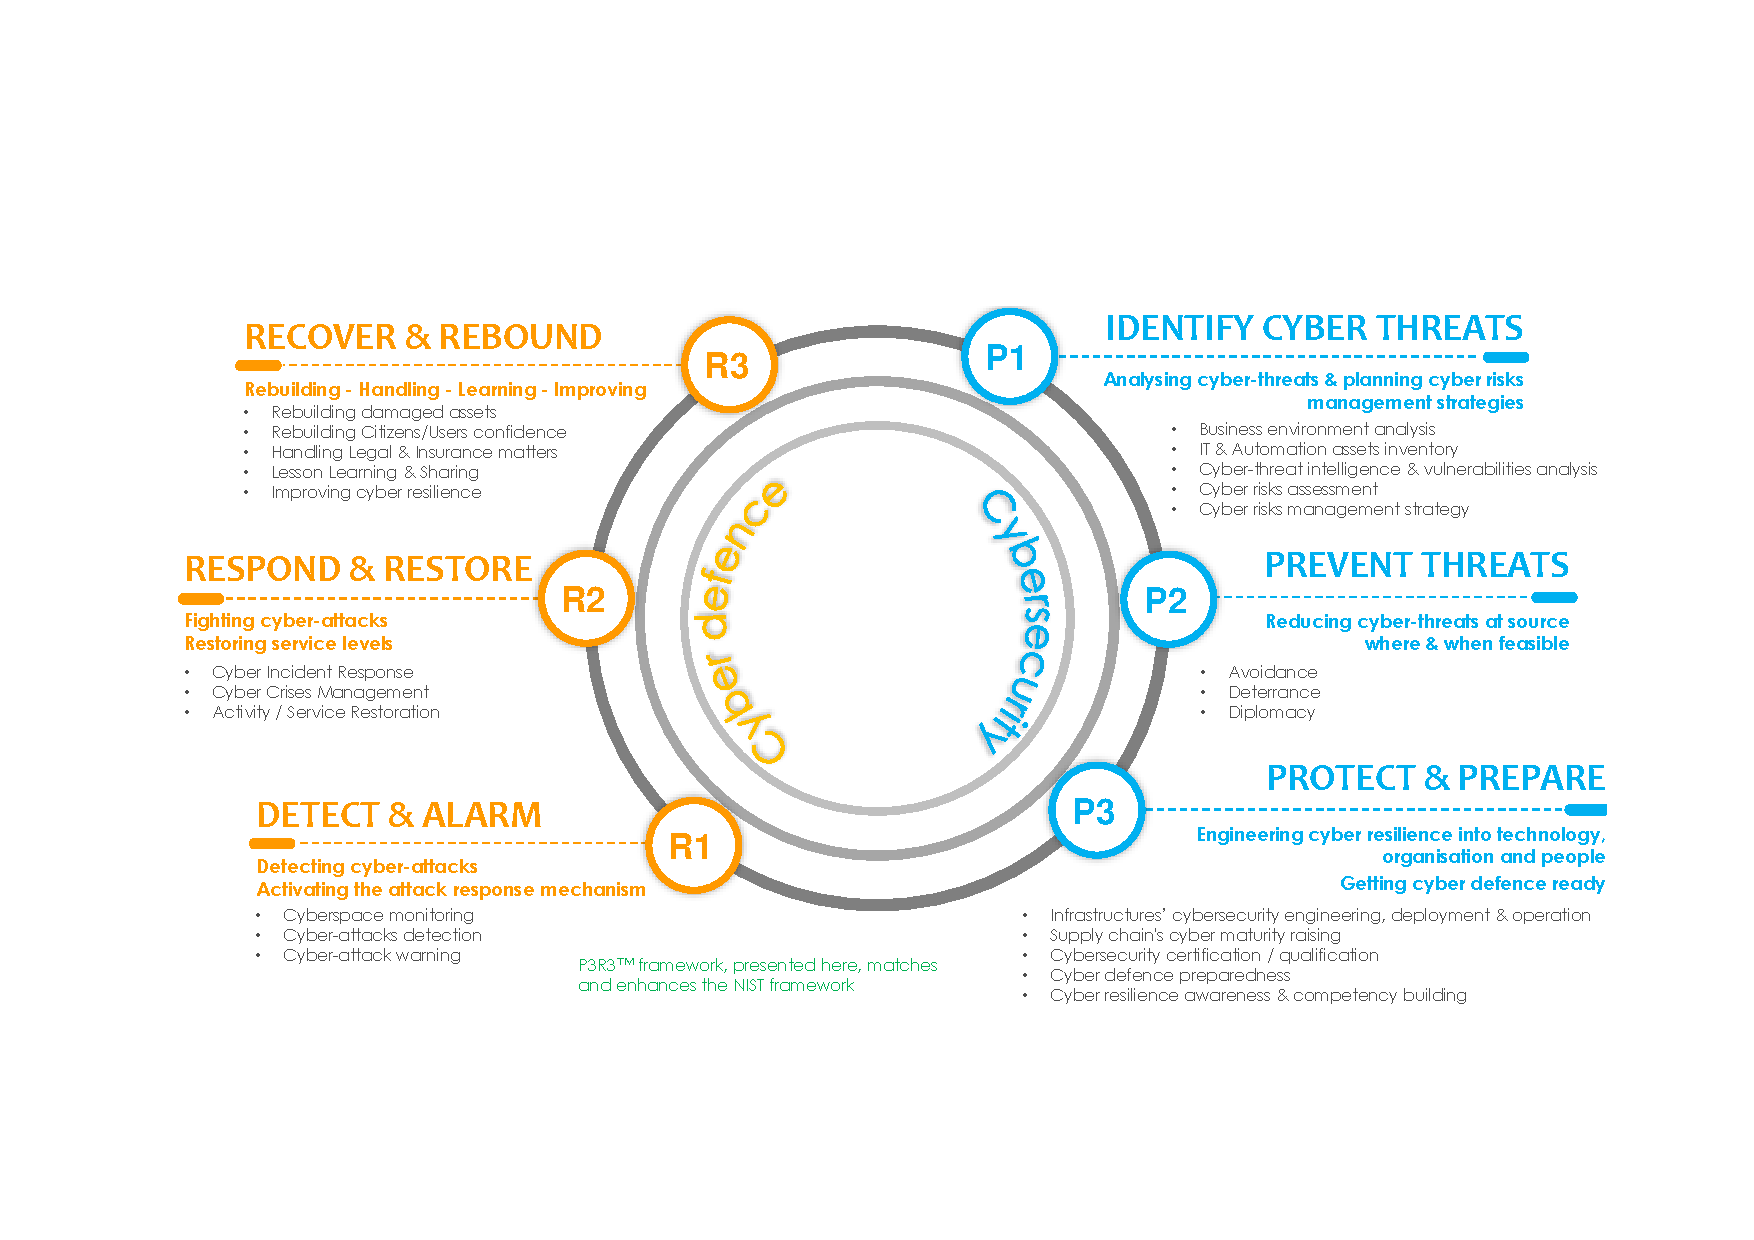
\includegraphics[width=\linewidth]{figures/P3R3.pdf}
  \caption{Le modèle P3R3 pour la cyber-résilience (tiré de \autocite{Kott2023})}
  \label{fig:P3R3_model}
\end{figure}

\noindent
L'essentiel de la Cyber-résilience repose sur une combinaison de détection  et de réponse face aux cybermenaces. Toutefois, l'émergence de menaces toujours plus rapides, distribuées et intelligentes remet en cause les approches traditionnelles. C'est ce que nous explorons dans la section suivante, en analysant les évolutions récentes du paysage des cyberattaques et les défis associés à leur détection et leur neutralisation.


\section{Des menaces de plus en plus autonomes et distribuées}\label{sec:evolution-menaces}

Au cours des dernières années, l'écosystème des cybermenaces a subi une transformation majeure. L'arrivée de l'\acn{IA} agentique permet l'émergence d'attaques plus rapides, automatisées, adaptatives et opèrant en parallèle non seulement sur un hôte unique, mais sur des réseaux entiers~\cite{Cohen2020}. Des travaux récents montrent que des attaquants utilisent des \acn{LLM} pour générer des malwares, créer des campagnes de phishing ciblées, et réagir d'eux-mêmes aux systèmes de défense~\cite{AutoAttacker2024}. De tels systèmes permettent de déclencher des campagnes distribuées avec une vitesse et une efficacité très importante~\cite{AgenticAIThreats2025}.

\subsection*{Limites des approches classiques de la Cyberdéfense}

Les dispositifs de Cyberdéfense traditionnels (fondés sur des architectures centralisées, des signatures statiques ou des règles prédéfinies) sont aujourd'hui dépassés par cette nouvelle génération de menaces~\cite{Kott2023}~:
\begin{itemize}
  \item \textbf{Latence décisionnelle}~: la centralisation de la détection engendre des délais critiques, permettant à certaines attaques de se produire avant même qu’elles ne soient identifiées et traitées par les équipes de Cyberdéfense~;
  \item \textbf{Rigidité adaptative}~: des règles statiques ne peuvent suivre l'évolution des modes opératoires des attaquants~;
  \item \textbf{Peu de résilience}~: lorsqu'une attaque est détectée, aucune action corrective immédiate n'est engagée. Cela retarde la restauration du système et laisse les conséquences de l'incident s'aggraver, limitant ainsi l'efficacité de la réponse post-attaque.
\end{itemize}

Ces limites identifiées soulignent la nécessité d'un paradigme plus agile, proactif et intelligent dans la Cyberdéfense. Des études récentes identifient l'avènement d'attaques basées sur l'\acn{IA}~\cite{Miles2018,AutoAttacker2024,Falong2025}, où les agents malveillants~:
\begin{itemize}
  \item \textbf{Automatisent} la recherche de vulnérabilités, le déploiement de charges utiles, et l'exfiltration~;
  \item \textbf{Coopèrent} en coordonnant des vecteurs d'attaque parallèles décrits dans les modèles de multi-agents adverses~;
  \item \textbf{Exploitent} des techniques d'\textbf{adversarial ML}, générant des formes d'échappement aux detections habituelles (poisoning, prompt injection…).
\end{itemize}

\subsection*{Une approche autonome de Cyberdéfense}

Pour faire face à ces menaces, le domaine émergent de l'\acn{ACO} cherche à développer des systèmes capables de prendre des décisions complexes de manière autonome, en tenant compte du contexte, des objectifs à atteindre et des conséquences possibles de leurs actions, le tout en temps réel et avec une supervision humaine minimale, voire inexistante~\cite{Vyas2023}. Les premiers travaux dans ce domaine portent principalement sur des architectures à base d'agents logiciels autonomes, en particulier dans le cadre du groupe \textit{IST-152} de l'\acn{OTAN}, à l'origine du concept d'agent \acn{AICA}.
Un tel agent est théorisé comme étant capable de percevoir son environnement local (par l'analyse de journaux, de flux ou d'heuristiques), de prendre des décisions autonomes en s'appuyant sur des règles ou des mécanismes d'apprentissage, d'agir localement (par exemple via des actions de filtrage ou d'isolement) sans dépendre d'un contrôle externe permanent, et enfin de communiquer avec d'autres agents ou des opérateurs humains afin de partager des indicateurs, des intentions ou des états.

Dans ce cadre, l'architecture modulaire \acn{MASCARA}, illustrée en \autoref{fig:mascara}, a été introduite pour formaliser le fonctionnement interne d'un agent \acn{AICA} en décomposant ses activités en plusieurs modules spécialisés~: collecte de journaux, détection d'anomalies, sélection de contre-mesures, application des réponses, etc. En s'appuyant sur cette architecture générale, il devient possible de concevoir une instance concrète adaptée à un environnement spécifique, en modulant le nombre de composants, leur nature et leurs interactions. Une telle adaptation permet à l'agent \acn{AICA} de répondre finement aux exigences de son contexte de déploiement et de garantir une protection {\em en edge}, c'est-à-dire au plus proche des ressources à défendre, tout en optimisant la performance dans l'atteinte des objectifs de Cyberdéfense.

Cependant, cette architecture reste fondamentalement monolithique et figée. Elle ne fournit pas, en l'état, les moyens d'adaptation nécessaires pour faire face aux dynamiques imprévisibles d'un environnement opérationnel réel, en particulier dans le cadre de systèmes distribués, complexes et fortement interactifs. Cette rigidité limite significativement la capacité d'un agent \acn{AICA} à réagir à l'émergence de nouvelles menaces ou à s'ajuster aux contraintes environnementales fluctuantes.


\begin{figure}[h!]
  \centering
  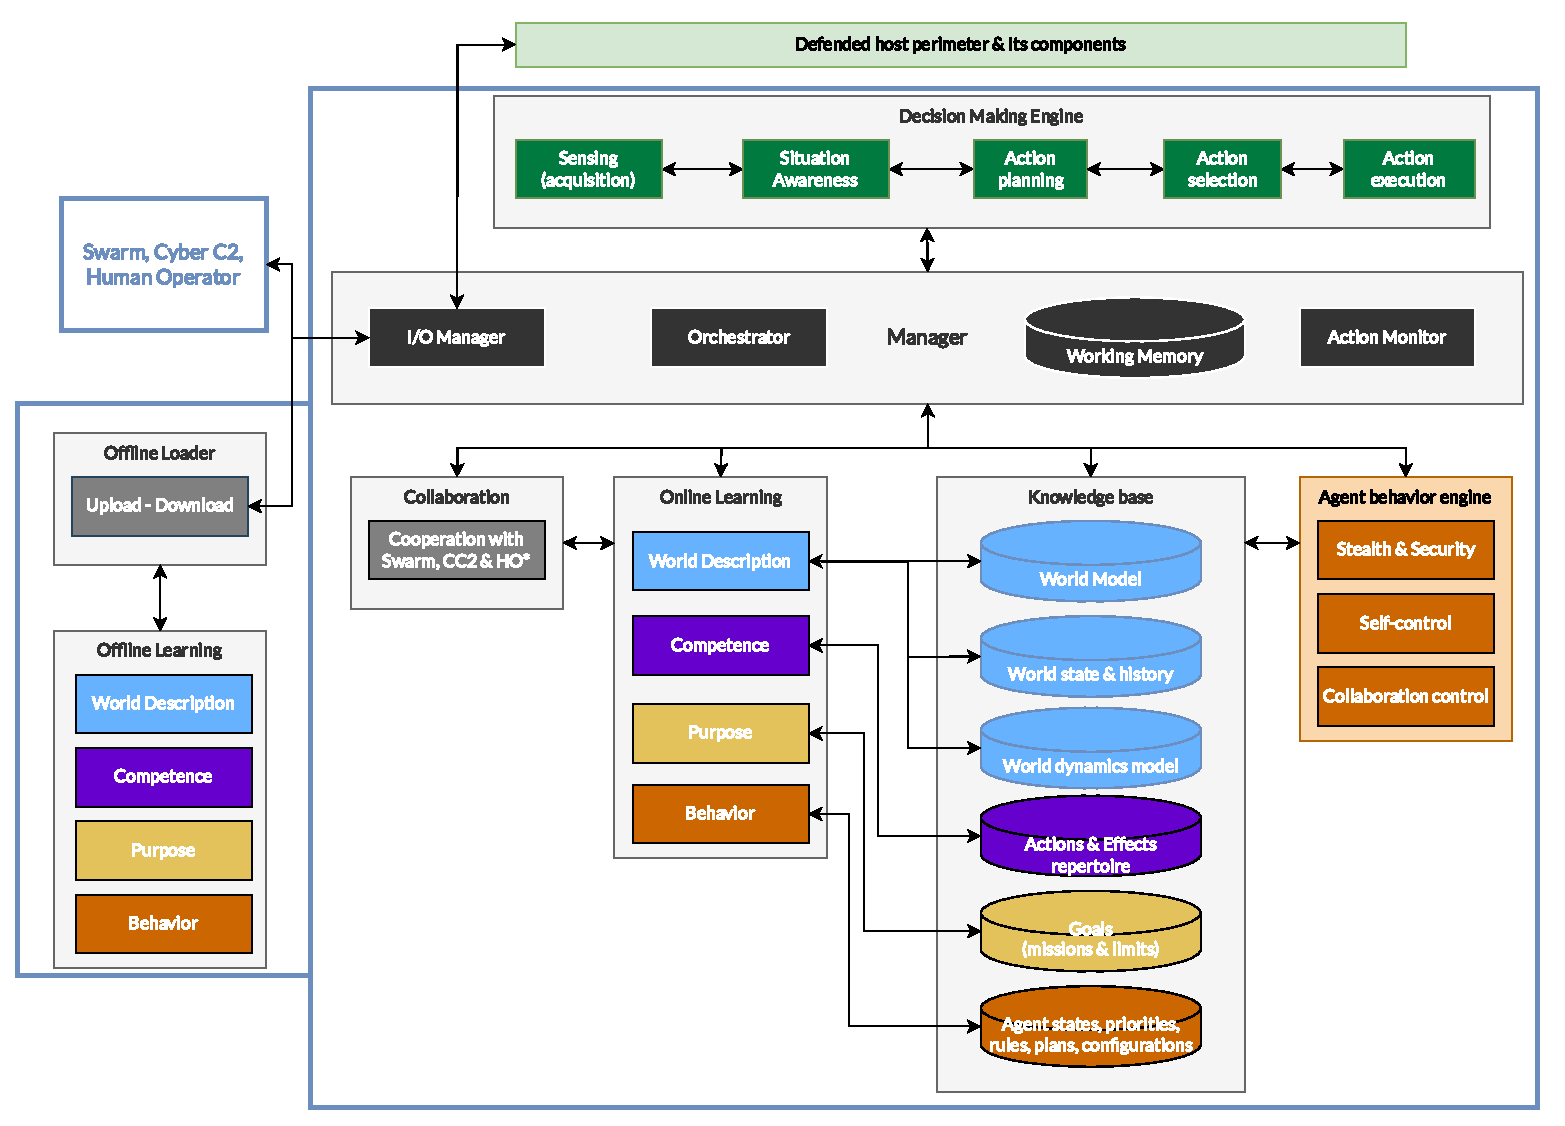
\includegraphics[width=\linewidth]{figures/MASCARA.pdf}
  \caption{Description de l'architecture modulaire MASCARA (tirée de \autocite{Kott2023})}
  \label{fig:mascara}
\end{figure}

\subsection*{Vers des approches coopératives}

La simple composition modulaire proposée initialement ne suffit plus à répondre à la complexité croissante des infrastructures critiques actuelles. Celle-ci impose l'adoption d'un paradigme distribué, dans lequel plusieurs agents interconnectés coopèrent, s'auto-organisent et se réorganisent dynamiquement en fonction des besoins opérationnels~\cite{Ferber1999, Gleizes2008}. Dans cette perspective, l'idée a émergé de transformer chaque module de l'architecture \acn{MASCARA} en un agent autonome, chargé d'exécuter une tâche spécifique de Cyberdéfense. Ces micro-agents, en interagissant de manière coordonnée, permettraient de mieux répartir les responsabilités, de renforcer la robustesse du système et d'atteindre collectivement les objectifs globaux de protection.

La notion de granularité permet ici d'opérer une distinction entre les micro-agents, chacun dédié à une fonction bien définie, et les agents \acn{AICA} dits complets, capables de couvrir l'ensemble des missions prévues par le modèle. Dans la suite de ce manuscrit, nous emploierons le terme générique d'agent \acn{AICA} pour désigner ces deux types d'agents, en précisant systématiquement le périmètre fonctionnel concerné selon le contexte.

Plus généralement, cette approche distribuée et coopérative s'inscrit dans une vision systémique de la Cyberdéfense, dans laquelle un ensemble d'agents autonomes interagit au sein du réseau pour garantir une sécurité globale, adaptative et résiliente. Cette orientation conceptuelle est soutenue par plusieurs travaux récents appartenant au domaine récent de l'\acn{ACD}~\cite{Vyas2023} (un sous domaine de l'\acparen{ACO}) et constitue un fondement essentiel des développements présentés dans ce manuscrit.


Par exemple, des simulations ont montré que des équipes d'agents défensifs sont capables de surpasser un agent unique en termes de couverture du réseau et de réactivité, grâce à une coordination dynamique et distribuée~\cite{RLResilientCyberdefense2024}.
Des plateformes telles que \textit{CybORG}~\cite{cage_challenge_3_announcement} illustrent également cette tendance, en proposant un environnement simulé dans lequel des agents autonomes décentralisés défendent simultanément un réseau face à des attaques coordonnées.

L'approche coopérative permet non seulement de protéger plusieurs hôtes en parallèle, mais aussi de détecter des attaques synchronisées et de s'adapter dynamiquement aux changements de topologie du réseau. Elle pose ainsi les bases d'une Cyberdéfense distribuée, proactive et évolutive, en rupture avec les architectures défensives traditionnelles.

\begin{figure}[h]
  \centering
  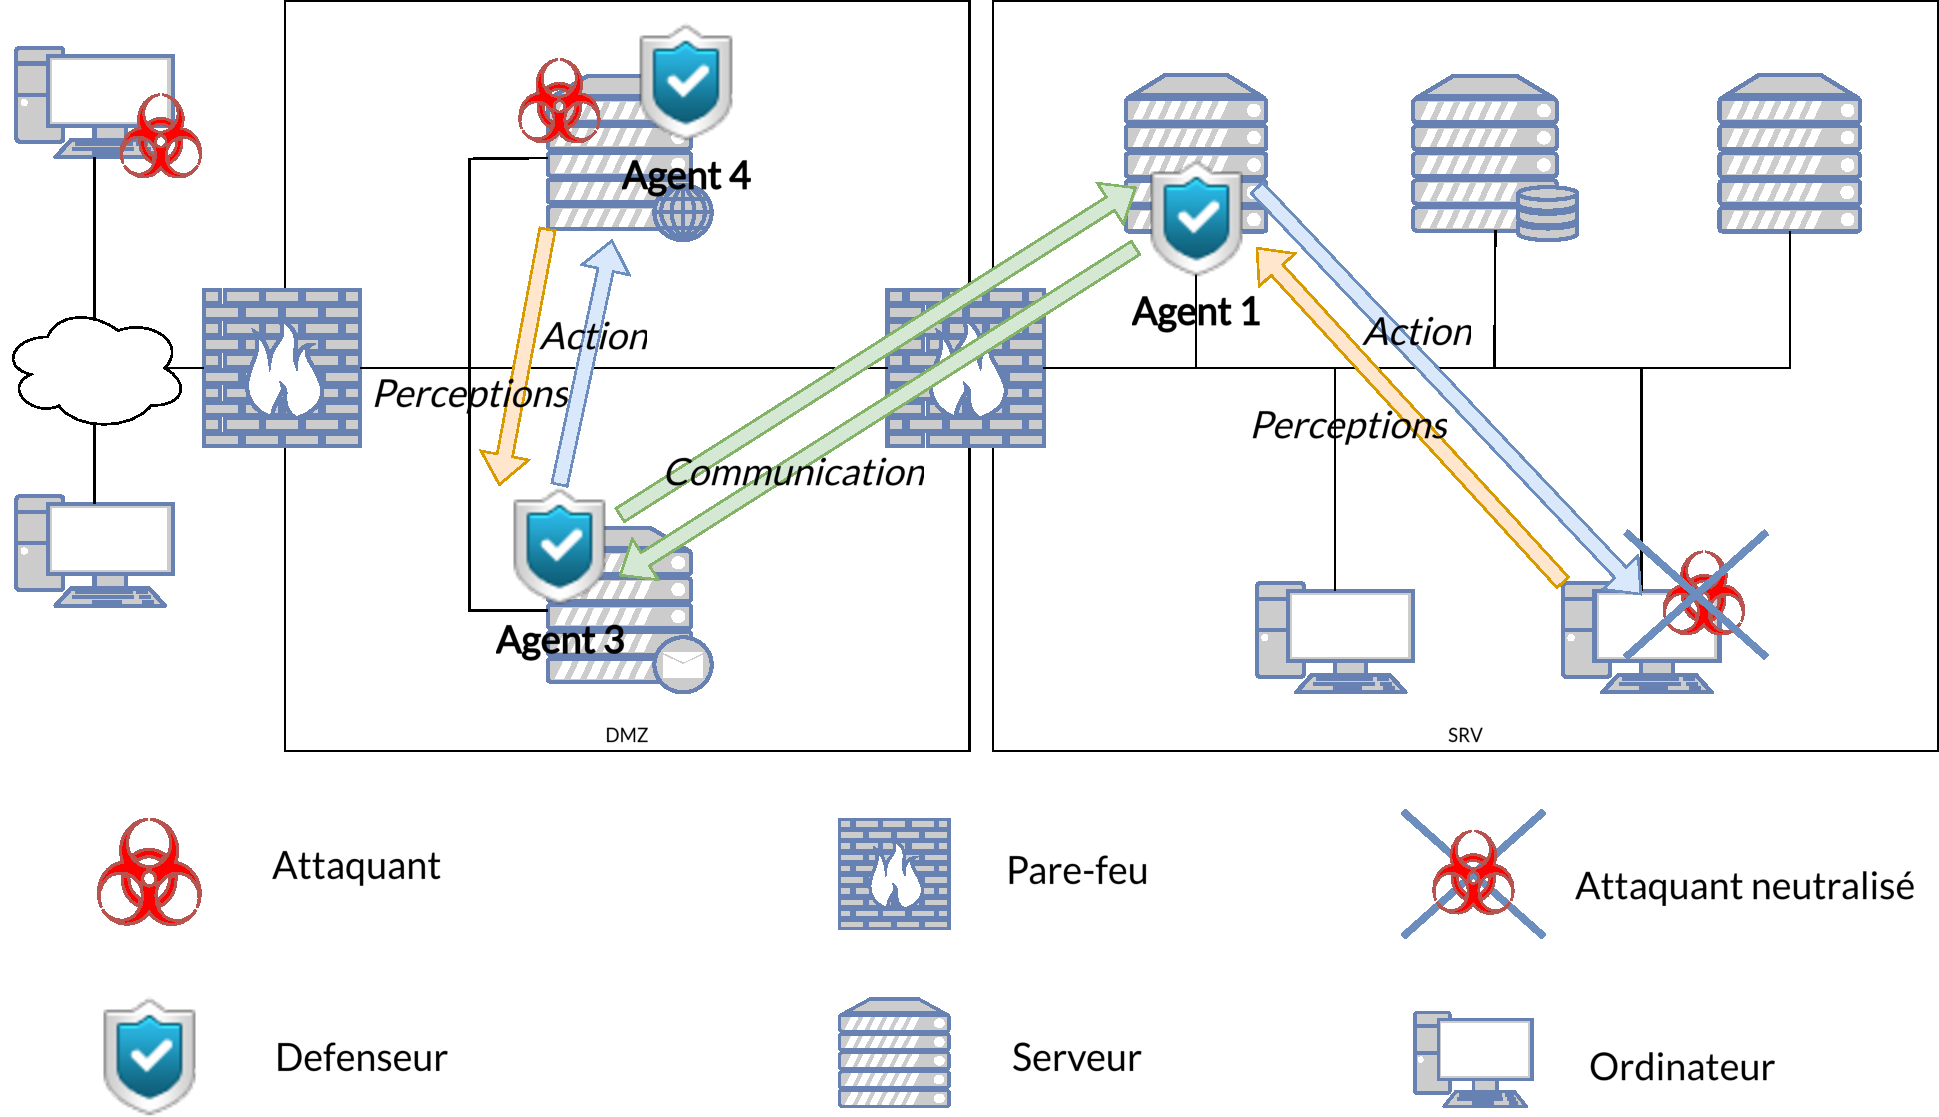
\includegraphics[width=\linewidth]{figures/infra_MAS_illustration.pdf}
  \caption{Illustration schématique d'un SMA de Cyberdéfense dans une infrastructure d'entreprise jouet}
  \label{fig:distributed_sma}
\end{figure}

\noindent
Finalement, c'est dans ce contexte que l'idée d'un \acn{SMA} de Cyberdéfense, tel que illustré dans \autoref{fig:distributed_sma}, apparaît comme une alternative générique prometteuse par rapport aux approches centralisées existantes. Nous présentons dans la section suivante les bases conceptuelles des \acn{SMA} en vue de la conception d'un \acn{SMA} de Cyberdéfense.

\section{La piste d'une vision multi-agent}\label{sec:sma-concepts}

Les \acn{SMA} constituent un paradigme central de l'\acn{IA} distribuée. Ils permettent de concevoir des systèmes complexes à partir d'agents autonomes interagissant dans un environnement partagé. Ces agents peuvent percevoir, raisonner, décider et agir de manière coordonnée pour résoudre des problèmes collectifs~\cite{Ferber1999,Wooldridge2002}.

\subsection*{Définitions fondamentales}

Un \textbf{agent} est une entité autonome, physique ou logicielle, capable de percevoir son environnement, de prendre des décisions et d'agir pour atteindre des objectifs~\cite{Russell2010}. Comme illustré dans \autoref{fig:sma_illustration}, un \acn{SMA} regroupe plusieurs de ces agents qui coopèrent ou interagissent au sein d’un environnement généralement dynamique et partiellement observable~\cite{Jennings1998,Shoham2007}. Chaque agent dispose d’une \emph{zone d’observation locale} (disque pointillé) lui permettant de percevoir uniquement une partie de l’environnement et des autres entités. À partir de ces observations partielles, et selon des \emph{stratégies ou politiques} (schéma en haut de la figure), il sélectionne et exécute des \emph{actions} dirigées vers des composants de l’environnement (carrés) ou vers d’autres agents (flèches pleines). Les agents peuvent également \emph{échanger des messages} (flèches en tirets) afin de coordonner leurs comportements. L’objectif global (en haut à droite) représente un état souhaité de l’environnement que les agents cherchent à atteindre collectivement.

\begin{figure}[h]
  \centering
  \resizebox{\textwidth}{!}{%
    


\tikzset{every picture/.style={line width=0.75pt}} %set default line width to 0.75pt        

\begin{tikzpicture}[x=0.75pt,y=0.75pt,yscale=-1,xscale=1]
%uncomment if require: \path (0,1498); %set diagram left start at 0, and has height of 1498

%Rounded Rect [id:dp8571088761489256] 
\draw  [fill={rgb, 255:red, 255; green, 255; blue, 255 }  ,fill opacity=1 ] (195,482.84) .. controls (195,478.51) and (198.51,475) .. (202.84,475) -- (632.16,475) .. controls (636.49,475) and (640,478.51) .. (640,482.84) -- (640,752.16) .. controls (640,756.49) and (636.49,760) .. (632.16,760) -- (202.84,760) .. controls (198.51,760) and (195,756.49) .. (195,752.16) -- cycle ;
%Shape: Smiley Face [id:dp9608565483930217] 
\draw  [fill={rgb, 255:red, 208; green, 2; blue, 27 }  ,fill opacity=1 ] (276.44,575.59) .. controls (276.44,569.59) and (281.41,564.72) .. (287.53,564.72) .. controls (293.66,564.72) and (298.63,569.59) .. (298.63,575.59) .. controls (298.63,581.59) and (293.66,586.46) .. (287.53,586.46) .. controls (281.41,586.46) and (276.44,581.59) .. (276.44,575.59) -- cycle ; \draw  [fill={rgb, 255:red, 208; green, 2; blue, 27 }  ,fill opacity=1 ] (282.65,571.89) .. controls (282.65,571.29) and (283.15,570.81) .. (283.76,570.81) .. controls (284.37,570.81) and (284.87,571.29) .. (284.87,571.89) .. controls (284.87,572.49) and (284.37,572.98) .. (283.76,572.98) .. controls (283.15,572.98) and (282.65,572.49) .. (282.65,571.89) -- cycle ; \draw  [fill={rgb, 255:red, 208; green, 2; blue, 27 }  ,fill opacity=1 ] (290.2,571.89) .. controls (290.2,571.29) and (290.69,570.81) .. (291.31,570.81) .. controls (291.92,570.81) and (292.42,571.29) .. (292.42,571.89) .. controls (292.42,572.49) and (291.92,572.98) .. (291.31,572.98) .. controls (290.69,572.98) and (290.2,572.49) .. (290.2,571.89) -- cycle ; \draw   (281.99,579.94) .. controls (285.69,582.84) and (289.38,582.84) .. (293.08,579.94) ;
%Rounded Rect [id:dp759927621160896] 
\draw  [fill={rgb, 255:red, 80; green, 227; blue, 194 }  ,fill opacity=1 ] (333.1,562.39) .. controls (333.1,559.2) and (335.69,556.62) .. (338.87,556.62) -- (356.18,556.62) .. controls (359.37,556.62) and (361.95,559.2) .. (361.95,562.39) -- (361.95,580.06) .. controls (361.95,583.25) and (359.37,585.83) .. (356.18,585.83) -- (338.87,585.83) .. controls (335.69,585.83) and (333.1,583.25) .. (333.1,580.06) -- cycle ;
%Rounded Rect [id:dp3032709932069614] 
\draw  [fill={rgb, 255:red, 74; green, 144; blue, 226 }  ,fill opacity=1 ] (212.19,530.72) .. controls (212.19,527.54) and (214.77,524.95) .. (217.96,524.95) -- (235.26,524.95) .. controls (238.45,524.95) and (241.03,527.54) .. (241.03,530.72) -- (241.03,548.4) .. controls (241.03,551.58) and (238.45,554.17) .. (235.26,554.17) -- (217.96,554.17) .. controls (214.77,554.17) and (212.19,551.58) .. (212.19,548.4) -- cycle ;
%Straight Lines [id:da31697688905948296] 
\draw    (276.94,570.08) -- (243,549.8) ;
\draw [shift={(240.42,548.26)}, rotate = 30.86] [fill={rgb, 255:red, 0; green, 0; blue, 0 }  ][line width=0.08]  [draw opacity=0] (5.36,-2.57) -- (0,0) -- (5.36,2.57) -- cycle    ;
%Straight Lines [id:da15166297291059583] 
\draw  [dash pattern={on 4.5pt off 4.5pt}]  (289.15,590.12) -- (287.45,663.28) ;
\draw [shift={(287.38,666.28)}, rotate = 271.33] [fill={rgb, 255:red, 0; green, 0; blue, 0 }  ][line width=0.08]  [draw opacity=0] (5.36,-2.57) -- (0,0) -- (5.36,2.57) -- cycle    ;
\draw [shift={(289.22,587.12)}, rotate = 91.33] [fill={rgb, 255:red, 0; green, 0; blue, 0 }  ][line width=0.08]  [draw opacity=0] (5.36,-2.57) -- (0,0) -- (5.36,2.57) -- cycle    ;
%Straight Lines [id:da19030240516000207] 
\draw  [dash pattern={on 4.5pt off 4.5pt}]  (433.57,605.62) -- (298.31,583.17) ;
\draw [shift={(295.36,582.68)}, rotate = 9.42] [fill={rgb, 255:red, 0; green, 0; blue, 0 }  ][line width=0.08]  [draw opacity=0] (5.36,-2.57) -- (0,0) -- (5.36,2.57) -- cycle    ;
\draw [shift={(436.53,606.12)}, rotate = 189.42] [fill={rgb, 255:red, 0; green, 0; blue, 0 }  ][line width=0.08]  [draw opacity=0] (5.36,-2.57) -- (0,0) -- (5.36,2.57) -- cycle    ;
%Straight Lines [id:da12208855578128797] 
\draw    (298.42,571.41) -- (330.43,567.88) ;
\draw [shift={(333.41,567.55)}, rotate = 173.7] [fill={rgb, 255:red, 0; green, 0; blue, 0 }  ][line width=0.08]  [draw opacity=0] (5.36,-2.57) -- (0,0) -- (5.36,2.57) -- cycle    ;
%Shape: Smiley Face [id:dp017117759022491463] 
\draw  [fill={rgb, 255:red, 126; green, 211; blue, 33 }  ,fill opacity=1 ] (277.98,676.13) .. controls (277.98,670.13) and (282.94,665.26) .. (289.07,665.26) .. controls (295.2,665.26) and (300.16,670.13) .. (300.16,676.13) .. controls (300.16,682.13) and (295.2,687) .. (289.07,687) .. controls (282.94,687) and (277.98,682.13) .. (277.98,676.13) -- cycle ; \draw  [fill={rgb, 255:red, 126; green, 211; blue, 33 }  ,fill opacity=1 ] (284.19,672.44) .. controls (284.19,671.84) and (284.68,671.35) .. (285.3,671.35) .. controls (285.91,671.35) and (286.41,671.84) .. (286.41,672.44) .. controls (286.41,673.04) and (285.91,673.52) .. (285.3,673.52) .. controls (284.68,673.52) and (284.19,673.04) .. (284.19,672.44) -- cycle ; \draw  [fill={rgb, 255:red, 126; green, 211; blue, 33 }  ,fill opacity=1 ] (291.73,672.44) .. controls (291.73,671.84) and (292.23,671.35) .. (292.84,671.35) .. controls (293.45,671.35) and (293.95,671.84) .. (293.95,672.44) .. controls (293.95,673.04) and (293.45,673.52) .. (292.84,673.52) .. controls (292.23,673.52) and (291.73,673.04) .. (291.73,672.44) -- cycle ; \draw   (283.52,680.48) .. controls (287.22,683.38) and (290.92,683.38) .. (294.62,680.48) ;
%Rounded Rect [id:dp2729577267316856] 
\draw  [fill={rgb, 255:red, 65; green, 117; blue, 5 }  ,fill opacity=1 ] (227.53,702.44) .. controls (227.53,699.25) and (230.11,696.67) .. (233.3,696.67) -- (250.61,696.67) .. controls (253.8,696.67) and (256.38,699.25) .. (256.38,702.44) -- (256.38,720.11) .. controls (256.38,723.3) and (253.8,725.88) .. (250.61,725.88) -- (233.3,725.88) .. controls (230.11,725.88) and (227.53,723.3) .. (227.53,720.11) -- cycle ;
%Rounded Rect [id:dp9608207589356206] 
\draw  [fill={rgb, 255:red, 184; green, 233; blue, 134 }  ,fill opacity=1 ] (471.21,734.1) .. controls (471.21,730.92) and (473.79,728.33) .. (476.98,728.33) -- (494.29,728.33) .. controls (497.47,728.33) and (500.06,730.92) .. (500.06,734.1) -- (500.06,751.78) .. controls (500.06,754.96) and (497.47,757.55) .. (494.29,757.55) -- (476.98,757.55) .. controls (473.79,757.55) and (471.21,754.96) .. (471.21,751.78) -- cycle ;
%Rounded Rect [id:dp2532918382479751] 
\draw  [fill={rgb, 255:red, 248; green, 231; blue, 28 }  ,fill opacity=1 ] (488.39,562.39) .. controls (488.39,559.2) and (490.98,556.62) .. (494.16,556.62) -- (511.47,556.62) .. controls (514.66,556.62) and (517.24,559.2) .. (517.24,562.39) -- (517.24,580.06) .. controls (517.24,583.25) and (514.66,585.83) .. (511.47,585.83) -- (494.16,585.83) .. controls (490.98,585.83) and (488.39,583.25) .. (488.39,580.06) -- cycle ;
%Rounded Rect [id:dp46841976175690214] 
\draw  [fill={rgb, 255:red, 74; green, 144; blue, 226 }  ,fill opacity=1 ] (593.97,654.94) .. controls (593.97,651.75) and (596.55,649.17) .. (599.74,649.17) -- (617.04,649.17) .. controls (620.23,649.17) and (622.81,651.75) .. (622.81,654.94) -- (622.81,672.61) .. controls (622.81,675.8) and (620.23,678.38) .. (617.04,678.38) -- (599.74,678.38) .. controls (596.55,678.38) and (593.97,675.8) .. (593.97,672.61) -- cycle ;
%Rounded Rect [id:dp35096543230819477] 
\draw  [fill={rgb, 255:red, 208; green, 2; blue, 27 }  ,fill opacity=1 ] (609.31,530.72) .. controls (609.31,527.54) and (611.89,524.95) .. (615.08,524.95) -- (632.39,524.95) .. controls (635.58,524.95) and (638.16,527.54) .. (638.16,530.72) -- (638.16,548.4) .. controls (638.16,551.58) and (635.58,554.17) .. (632.39,554.17) -- (615.08,554.17) .. controls (611.89,554.17) and (609.31,551.58) .. (609.31,548.4) -- cycle ;
%Rounded Rect [id:dp37268226656767] 
\draw  [fill={rgb, 255:red, 139; green, 87; blue, 42 }  ,fill opacity=1 ] (319.6,654.94) .. controls (319.6,651.75) and (322.18,649.17) .. (325.37,649.17) -- (342.68,649.17) .. controls (345.87,649.17) and (348.45,651.75) .. (348.45,654.94) -- (348.45,672.61) .. controls (348.45,675.8) and (345.87,678.38) .. (342.68,678.38) -- (325.37,678.38) .. controls (322.18,678.38) and (319.6,675.8) .. (319.6,672.61) -- cycle ;
%Shape: Smiley Face [id:dp8112481576921686] 
\draw  [fill={rgb, 255:red, 245; green, 166; blue, 35 }  ,fill opacity=1 ] (560.32,571.63) .. controls (560.32,565.63) and (565.29,560.76) .. (571.41,560.76) .. controls (577.54,560.76) and (582.51,565.63) .. (582.51,571.63) .. controls (582.51,577.63) and (577.54,582.5) .. (571.41,582.5) .. controls (565.29,582.5) and (560.32,577.63) .. (560.32,571.63) -- cycle ; \draw  [fill={rgb, 255:red, 245; green, 166; blue, 35 }  ,fill opacity=1 ] (566.53,567.94) .. controls (566.53,567.34) and (567.03,566.85) .. (567.64,566.85) .. controls (568.25,566.85) and (568.75,567.34) .. (568.75,567.94) .. controls (568.75,568.54) and (568.25,569.02) .. (567.64,569.02) .. controls (567.03,569.02) and (566.53,568.54) .. (566.53,567.94) -- cycle ; \draw  [fill={rgb, 255:red, 245; green, 166; blue, 35 }  ,fill opacity=1 ] (574.08,567.94) .. controls (574.08,567.34) and (574.57,566.85) .. (575.19,566.85) .. controls (575.8,566.85) and (576.29,567.34) .. (576.29,567.94) .. controls (576.29,568.54) and (575.8,569.02) .. (575.19,569.02) .. controls (574.57,569.02) and (574.08,568.54) .. (574.08,567.94) -- cycle ; \draw   (565.87,575.98) .. controls (569.56,578.88) and (573.26,578.88) .. (576.96,575.98) ;
%Shape: Smiley Face [id:dp26692841414623936] 
\draw  [fill={rgb, 255:red, 248; green, 231; blue, 28 }  ,fill opacity=1 ] (536.54,701.46) .. controls (536.54,695.46) and (541.5,690.6) .. (547.63,690.6) .. controls (553.76,690.6) and (558.72,695.46) .. (558.72,701.46) .. controls (558.72,707.47) and (553.76,712.33) .. (547.63,712.33) .. controls (541.5,712.33) and (536.54,707.47) .. (536.54,701.46) -- cycle ; \draw  [fill={rgb, 255:red, 248; green, 231; blue, 28 }  ,fill opacity=1 ] (542.75,697.77) .. controls (542.75,697.17) and (543.24,696.68) .. (543.86,696.68) .. controls (544.47,696.68) and (544.97,697.17) .. (544.97,697.77) .. controls (544.97,698.37) and (544.47,698.86) .. (543.86,698.86) .. controls (543.24,698.86) and (542.75,698.37) .. (542.75,697.77) -- cycle ; \draw  [fill={rgb, 255:red, 248; green, 231; blue, 28 }  ,fill opacity=1 ] (550.29,697.77) .. controls (550.29,697.17) and (550.79,696.68) .. (551.4,696.68) .. controls (552.01,696.68) and (552.51,697.17) .. (552.51,697.77) .. controls (552.51,698.37) and (552.01,698.86) .. (551.4,698.86) .. controls (550.79,698.86) and (550.29,698.37) .. (550.29,697.77) -- cycle ; \draw   (542.08,705.81) .. controls (545.78,708.71) and (549.48,708.71) .. (553.18,705.81) ;
%Shape: Smiley Face [id:dp13683684589232226] 
\draw  [fill={rgb, 255:red, 74; green, 144; blue, 226 }  ,fill opacity=1 ] (437.56,606.46) .. controls (437.56,600.46) and (442.53,595.6) .. (448.65,595.6) .. controls (454.78,595.6) and (459.75,600.46) .. (459.75,606.46) .. controls (459.75,612.47) and (454.78,617.33) .. (448.65,617.33) .. controls (442.53,617.33) and (437.56,612.47) .. (437.56,606.46) -- cycle ; \draw  [fill={rgb, 255:red, 74; green, 144; blue, 226 }  ,fill opacity=1 ] (443.77,602.77) .. controls (443.77,602.17) and (444.27,601.68) .. (444.88,601.68) .. controls (445.5,601.68) and (445.99,602.17) .. (445.99,602.77) .. controls (445.99,603.37) and (445.5,603.86) .. (444.88,603.86) .. controls (444.27,603.86) and (443.77,603.37) .. (443.77,602.77) -- cycle ; \draw  [fill={rgb, 255:red, 74; green, 144; blue, 226 }  ,fill opacity=1 ] (451.32,602.77) .. controls (451.32,602.17) and (451.81,601.68) .. (452.43,601.68) .. controls (453.04,601.68) and (453.54,602.17) .. (453.54,602.77) .. controls (453.54,603.37) and (453.04,603.86) .. (452.43,603.86) .. controls (451.81,603.86) and (451.32,603.37) .. (451.32,602.77) -- cycle ; \draw   (443.11,610.81) .. controls (446.81,613.71) and (450.5,613.71) .. (454.2,610.81) ;
%Shape: Ellipse [id:dp20697299562525007] 
\draw  [fill={rgb, 255:red, 126; green, 211; blue, 33 }  ,fill opacity=0.2 ][dash pattern={on 0.84pt off 2.51pt}] (240.81,675.7) .. controls (240.81,648.64) and (262.07,626.7) .. (288.3,626.7) .. controls (314.52,626.7) and (335.79,648.64) .. (335.79,675.7) .. controls (335.79,702.76) and (314.52,724.7) .. (288.3,724.7) .. controls (262.07,724.7) and (240.81,702.76) .. (240.81,675.7) -- cycle ;
%Shape: Ellipse [id:dp5331145075645709] 
\draw  [fill={rgb, 255:red, 248; green, 231; blue, 28 }  ,fill opacity=0.2 ][dash pattern={on 0.84pt off 2.51pt}] (488.09,699.99) .. controls (488.09,667.29) and (513.78,640.78) .. (545.47,640.78) .. controls (577.17,640.78) and (602.86,667.29) .. (602.86,699.99) .. controls (602.86,732.7) and (577.17,759.21) .. (545.47,759.21) .. controls (513.78,759.21) and (488.09,732.7) .. (488.09,699.99) -- cycle ;
%Shape: Ellipse [id:dp1108681712787154] 
\draw  [fill={rgb, 255:red, 74; green, 144; blue, 226 }  ,fill opacity=0.2 ][dash pattern={on 0.84pt off 2.51pt}] (367.55,608.99) .. controls (367.55,564.02) and (402.88,527.57) .. (446.46,527.57) .. controls (490.04,527.57) and (525.37,564.02) .. (525.37,608.99) .. controls (525.37,653.96) and (490.04,690.41) .. (446.46,690.41) .. controls (402.88,690.41) and (367.55,653.96) .. (367.55,608.99) -- cycle ;
%Shape: Ellipse [id:dp35349211767213196] 
\draw  [fill={rgb, 255:red, 245; green, 166; blue, 35 }  ,fill opacity=0.2 ][dash pattern={on 0.84pt off 2.51pt}] (511.87,570.16) .. controls (511.87,537.46) and (537.56,510.95) .. (569.26,510.95) .. controls (600.95,510.95) and (626.65,537.46) .. (626.65,570.16) .. controls (626.65,602.86) and (600.95,629.38) .. (569.26,629.38) .. controls (537.56,629.38) and (511.87,602.86) .. (511.87,570.16) -- cycle ;
%Straight Lines [id:da868926834515953] 
\draw    (299.65,673.88) -- (315.99,672.69) ;
\draw [shift={(318.99,672.47)}, rotate = 175.83] [fill={rgb, 255:red, 0; green, 0; blue, 0 }  ][line width=0.08]  [draw opacity=0] (5.36,-2.57) -- (0,0) -- (5.36,2.57) -- cycle    ;
%Straight Lines [id:da7856168052805825] 
\draw    (458.62,601.05) -- (490.69,586.98) ;
\draw [shift={(493.44,585.77)}, rotate = 156.31] [fill={rgb, 255:red, 0; green, 0; blue, 0 }  ][line width=0.08]  [draw opacity=0] (5.36,-2.57) -- (0,0) -- (5.36,2.57) -- cycle    ;
%Straight Lines [id:da9445808525599552] 
\draw    (580.77,564.32) -- (605.66,552.9) ;
\draw [shift={(608.39,551.65)}, rotate = 155.36] [fill={rgb, 255:red, 0; green, 0; blue, 0 }  ][line width=0.08]  [draw opacity=0] (5.36,-2.57) -- (0,0) -- (5.36,2.57) -- cycle    ;
%Straight Lines [id:da12131692830119956] 
\draw    (558.67,698.58) -- (592.93,677.96) ;
\draw [shift={(595.5,676.42)}, rotate = 148.96] [fill={rgb, 255:red, 0; green, 0; blue, 0 }  ][line width=0.08]  [draw opacity=0] (5.36,-2.57) -- (0,0) -- (5.36,2.57) -- cycle    ;
%Straight Lines [id:da02866326716436185] 
\draw    (539.64,709.98) -- (502.01,732.57) ;
\draw [shift={(499.44,734.11)}, rotate = 329.03] [fill={rgb, 255:red, 0; green, 0; blue, 0 }  ][line width=0.08]  [draw opacity=0] (5.36,-2.57) -- (0,0) -- (5.36,2.57) -- cycle    ;
%Straight Lines [id:da3852011537026049] 
\draw  [dash pattern={on 4.5pt off 4.5pt}]  (458.31,616.46) -- (536.28,693.31) ;
\draw [shift={(538.42,695.42)}, rotate = 224.59] [fill={rgb, 255:red, 0; green, 0; blue, 0 }  ][line width=0.08]  [draw opacity=0] (5.36,-2.57) -- (0,0) -- (5.36,2.57) -- cycle    ;
\draw [shift={(456.17,614.35)}, rotate = 44.59] [fill={rgb, 255:red, 0; green, 0; blue, 0 }  ][line width=0.08]  [draw opacity=0] (5.36,-2.57) -- (0,0) -- (5.36,2.57) -- cycle    ;
%Straight Lines [id:da9204270310799157] 
\draw  [dash pattern={on 4.5pt off 4.5pt}]  (550.02,686.77) -- (569.17,585) ;
\draw [shift={(569.72,582.05)}, rotate = 100.65] [fill={rgb, 255:red, 0; green, 0; blue, 0 }  ][line width=0.08]  [draw opacity=0] (5.36,-2.57) -- (0,0) -- (5.36,2.57) -- cycle    ;
\draw [shift={(549.47,689.72)}, rotate = 280.65] [fill={rgb, 255:red, 0; green, 0; blue, 0 }  ][line width=0.08]  [draw opacity=0] (5.36,-2.57) -- (0,0) -- (5.36,2.57) -- cycle    ;
%Straight Lines [id:da9548969852220758] 
\draw    (576.47,581.42) -- (605.92,646.45) ;
\draw [shift={(607.16,649.18)}, rotate = 245.64] [fill={rgb, 255:red, 0; green, 0; blue, 0 }  ][line width=0.08]  [draw opacity=0] (5.36,-2.57) -- (0,0) -- (5.36,2.57) -- cycle    ;
%Shape: Ellipse [id:dp5345394122462545] 
\draw  [fill={rgb, 255:red, 208; green, 2; blue, 27 }  ,fill opacity=0.2 ][dash pattern={on 0.84pt off 2.51pt}] (203.9,573.33) .. controls (203.9,525.58) and (241.41,486.88) .. (287.68,486.88) .. controls (333.95,486.88) and (371.47,525.58) .. (371.47,573.33) .. controls (371.47,621.07) and (333.95,659.78) .. (287.68,659.78) .. controls (241.41,659.78) and (203.9,621.07) .. (203.9,573.33) -- cycle ;
%Rounded Rect [id:dp14561871899929513] 
\draw  [fill={rgb, 255:red, 155; green, 155; blue, 155 }  ,fill opacity=1 ] (36,644) .. controls (36,641.79) and (37.79,640) .. (40,640) -- (52,640) .. controls (54.21,640) and (56,641.79) .. (56,644) -- (56,656) .. controls (56,658.21) and (54.21,660) .. (52,660) -- (40,660) .. controls (37.79,660) and (36,658.21) .. (36,656) -- cycle ;
%Shape: Circle [id:dp8389216043634751] 
\draw  [dash pattern={on 0.84pt off 2.51pt}] (40,542) .. controls (40,536.48) and (44.48,532) .. (50,532) .. controls (55.52,532) and (60,536.48) .. (60,542) .. controls (60,547.52) and (55.52,552) .. (50,552) .. controls (44.48,552) and (40,547.52) .. (40,542) -- cycle ;
%Rounded Rect [id:dp1716372782625939] 
\draw  [fill={rgb, 255:red, 255; green, 255; blue, 255 }  ,fill opacity=1 ] (530,401.51) .. controls (530,400.68) and (530.68,400) .. (531.51,400) -- (608.49,400) .. controls (609.32,400) and (610,400.68) .. (610,401.51) -- (610,453.49) .. controls (610,454.32) and (609.32,455) .. (608.49,455) -- (531.51,455) .. controls (530.68,455) and (530,454.32) .. (530,453.49) -- cycle ;
%Rounded Rect [id:dp8384348356925067] 
\draw  [fill={rgb, 255:red, 80; green, 227; blue, 194 }  ,fill opacity=1 ] (553.51,417.41) .. controls (553.51,416.82) and (553.99,416.34) .. (554.57,416.34) -- (557.77,416.34) .. controls (558.35,416.34) and (558.83,416.82) .. (558.83,417.41) -- (558.83,420.96) .. controls (558.83,421.55) and (558.35,422.03) .. (557.77,422.03) -- (554.57,422.03) .. controls (553.99,422.03) and (553.51,421.55) .. (553.51,420.96) -- cycle ;
%Rounded Rect [id:dp32115157665477156] 
\draw  [fill={rgb, 255:red, 65; green, 117; blue, 5 }  ,fill opacity=1 ] (534.04,444.66) .. controls (534.04,444.07) and (534.52,443.59) .. (535.1,443.59) -- (538.3,443.59) .. controls (538.88,443.59) and (539.36,444.07) .. (539.36,444.66) -- (539.36,448.21) .. controls (539.36,448.8) and (538.88,449.28) .. (538.3,449.28) -- (535.1,449.28) .. controls (534.52,449.28) and (534.04,448.8) .. (534.04,448.21) -- cycle ;
%Rounded Rect [id:dp8306304589808061] 
\draw  [fill={rgb, 255:red, 184; green, 233; blue, 134 }  ,fill opacity=1 ] (579.52,448.07) .. controls (579.52,447.48) and (580,447) .. (580.59,447) -- (583.78,447) .. controls (584.37,447) and (584.84,447.48) .. (584.84,448.07) -- (584.84,451.62) .. controls (584.84,452.21) and (584.37,452.69) .. (583.78,452.69) -- (580.59,452.69) .. controls (580,452.69) and (579.52,452.21) .. (579.52,451.62) -- cycle ;
%Rounded Rect [id:dp36124132336547066] 
\draw  [fill={rgb, 255:red, 248; green, 231; blue, 28 }  ,fill opacity=1 ] (582.15,417.41) .. controls (582.15,416.82) and (582.63,416.34) .. (583.21,416.34) -- (586.41,416.34) .. controls (586.99,416.34) and (587.47,416.82) .. (587.47,417.41) -- (587.47,420.96) .. controls (587.47,421.55) and (586.99,422.03) .. (586.41,422.03) -- (583.21,422.03) .. controls (582.63,422.03) and (582.15,421.55) .. (582.15,420.96) -- cycle ;
%Rounded Rect [id:dp07486815562281168] 
\draw  [fill={rgb, 255:red, 74; green, 144; blue, 226 }  ,fill opacity=1 ] (601.62,435.41) .. controls (601.62,434.83) and (602.1,434.35) .. (602.68,434.35) -- (605.88,434.35) .. controls (606.46,434.35) and (606.94,434.83) .. (606.94,435.41) -- (606.94,438.97) .. controls (606.94,439.56) and (606.46,440.03) .. (605.88,440.03) -- (602.68,440.03) .. controls (602.1,440.03) and (601.62,439.56) .. (601.62,438.97) -- cycle ;
%Rounded Rect [id:dp30447435501798137] 
\draw  [fill={rgb, 255:red, 74; green, 144; blue, 226 }  ,fill opacity=1 ] (531.21,411.24) .. controls (531.21,410.66) and (531.69,410.18) .. (532.27,410.18) -- (535.47,410.18) .. controls (536.05,410.18) and (536.53,410.66) .. (536.53,411.24) -- (536.53,414.8) .. controls (536.53,415.39) and (536.05,415.86) .. (535.47,415.86) -- (532.27,415.86) .. controls (531.69,415.86) and (531.21,415.39) .. (531.21,414.8) -- cycle ;
%Rounded Rect [id:dp9375364402563595] 
\draw  [fill={rgb, 255:red, 208; green, 2; blue, 27 }  ,fill opacity=1 ] (604.45,411.24) .. controls (604.45,410.66) and (604.93,410.18) .. (605.51,410.18) -- (608.71,410.18) .. controls (609.29,410.18) and (609.77,410.66) .. (609.77,411.24) -- (609.77,414.8) .. controls (609.77,415.39) and (609.29,415.86) .. (608.71,415.86) -- (605.51,415.86) .. controls (604.93,415.86) and (604.45,415.39) .. (604.45,414.8) -- cycle ;
%Rounded Rect [id:dp7769696093588394] 
\draw  [fill={rgb, 255:red, 139; green, 87; blue, 42 }  ,fill opacity=1 ] (551.02,435.41) .. controls (551.02,434.83) and (551.5,434.35) .. (552.08,434.35) -- (555.28,434.35) .. controls (555.86,434.35) and (556.34,434.83) .. (556.34,435.41) -- (556.34,438.97) .. controls (556.34,439.56) and (555.86,440.03) .. (555.28,440.03) -- (552.08,440.03) .. controls (551.5,440.03) and (551.02,439.56) .. (551.02,438.97) -- cycle ;
%Straight Lines [id:da7689335282153781] 
\draw    (35,711) -- (52,711) ;
\draw [shift={(55,711)}, rotate = 180] [fill={rgb, 255:red, 0; green, 0; blue, 0 }  ][line width=0.08]  [draw opacity=0] (5.36,-2.57) -- (0,0) -- (5.36,2.57) -- cycle    ;
%Shape: Boxed Line [id:dp5305044082643576] 
\draw  [dash pattern={on 4.5pt off 4.5pt}]  (38,598) -- (52,598) ;
\draw [shift={(55,598)}, rotate = 180] [fill={rgb, 255:red, 0; green, 0; blue, 0 }  ][line width=0.08]  [draw opacity=0] (5.36,-2.57) -- (0,0) -- (5.36,2.57) -- cycle    ;
\draw [shift={(35,598)}, rotate = 0] [fill={rgb, 255:red, 0; green, 0; blue, 0 }  ][line width=0.08]  [draw opacity=0] (5.36,-2.57) -- (0,0) -- (5.36,2.57) -- cycle    ;
%Rounded Rect [id:dp4866637287235507] 
\draw  [fill={rgb, 255:red, 128; green, 128; blue, 128 }  ,fill opacity=1 ] (417,412) .. controls (417,410.9) and (417.9,410) .. (419,410) -- (425,410) .. controls (426.1,410) and (427,410.9) .. (427,412) -- (427,418) .. controls (427,419.1) and (426.1,420) .. (425,420) -- (419,420) .. controls (417.9,420) and (417,419.1) .. (417,418) -- cycle ;
%Rounded Rect [id:dp6679922716487737] 
\draw  [fill={rgb, 255:red, 74; green, 144; blue, 226 }  ,fill opacity=1 ] (392,442) .. controls (392,440.9) and (392.9,440) .. (394,440) -- (400,440) .. controls (401.1,440) and (402,440.9) .. (402,442) -- (402,448) .. controls (402,449.1) and (401.1,450) .. (400,450) -- (394,450) .. controls (392.9,450) and (392,449.1) .. (392,448) -- cycle ;
%Rounded Rect [id:dp6398718898903711] 
\draw  [fill={rgb, 255:red, 208; green, 2; blue, 27 }  ,fill opacity=1 ] (427,442) .. controls (427,440.9) and (427.9,440) .. (429,440) -- (435,440) .. controls (436.1,440) and (437,440.9) .. (437,442) -- (437,448) .. controls (437,449.1) and (436.1,450) .. (435,450) -- (429,450) .. controls (427.9,450) and (427,449.1) .. (427,448) -- cycle ;
%Straight Lines [id:da4441060393578834] 
\draw [color={rgb, 255:red, 208; green, 2; blue, 27 }  ,draw opacity=1 ]   (422,420) -- (430.66,437.32) ;
\draw [shift={(432,440)}, rotate = 243.43] [fill={rgb, 255:red, 208; green, 2; blue, 27 }  ,fill opacity=1 ][line width=0.08]  [draw opacity=0] (5.36,-2.57) -- (0,0) -- (5.36,2.57) -- cycle    ;
%Rounded Rect [id:dp08606049626209744] 
\draw  [fill={rgb, 255:red, 248; green, 231; blue, 28 }  ,fill opacity=1 ] (442,442) .. controls (442,440.9) and (442.9,440) .. (444,440) -- (450,440) .. controls (451.1,440) and (452,440.9) .. (452,442) -- (452,448) .. controls (452,449.1) and (451.1,450) .. (450,450) -- (444,450) .. controls (442.9,450) and (442,449.1) .. (442,448) -- cycle ;
%Straight Lines [id:da5780422632856335] 
\draw [color={rgb, 255:red, 248; green, 231; blue, 28 }  ,draw opacity=1 ]   (422,420) -- (444.66,438.13) ;
\draw [shift={(447,440)}, rotate = 218.66] [fill={rgb, 255:red, 248; green, 231; blue, 28 }  ,fill opacity=1 ][line width=0.08]  [draw opacity=0] (5.36,-2.57) -- (0,0) -- (5.36,2.57) -- cycle    ;
%Straight Lines [id:da6560295978621367] 
\draw [color={rgb, 255:red, 74; green, 144; blue, 226 }  ,draw opacity=1 ]   (422,420) -- (399.34,438.13) ;
\draw [shift={(397,440)}, rotate = 321.34] [fill={rgb, 255:red, 74; green, 144; blue, 226 }  ,fill opacity=1 ][line width=0.08]  [draw opacity=0] (5.36,-2.57) -- (0,0) -- (5.36,2.57) -- cycle    ;
%Rounded Rect [id:dp8389325005978227] 
\draw  [fill={rgb, 255:red, 139; green, 87; blue, 42 }  ,fill opacity=1 ] (235,432) .. controls (235,430.9) and (235.9,430) .. (237,430) -- (243,430) .. controls (244.1,430) and (245,430.9) .. (245,432) -- (245,438) .. controls (245,439.1) and (244.1,440) .. (243,440) -- (237,440) .. controls (235.9,440) and (235,439.1) .. (235,438) -- cycle ;
%Rounded Rect [id:dp11911600050294124] 
\draw  [fill={rgb, 255:red, 74; green, 144; blue, 226 }  ,fill opacity=1 ] (245,447) .. controls (245,445.9) and (245.9,445) .. (247,445) -- (253,445) .. controls (254.1,445) and (255,445.9) .. (255,447) -- (255,453) .. controls (255,454.1) and (254.1,455) .. (253,455) -- (247,455) .. controls (245.9,455) and (245,454.1) .. (245,453) -- cycle ;
%Rounded Rect [id:dp6632279611422938] 
\draw  [fill={rgb, 255:red, 248; green, 231; blue, 28 }  ,fill opacity=1 ] (255,417) .. controls (255,415.9) and (255.9,415) .. (257,415) -- (263,415) .. controls (264.1,415) and (265,415.9) .. (265,417) -- (265,423) .. controls (265,424.1) and (264.1,425) .. (263,425) -- (257,425) .. controls (255.9,425) and (255,424.1) .. (255,423) -- cycle ;
%Rounded Rect [id:dp1401057934464146] 
\draw  [fill={rgb, 255:red, 208; green, 2; blue, 27 }  ,fill opacity=1 ] (265,432) .. controls (265,430.9) and (265.9,430) .. (267,430) -- (273,430) .. controls (274.1,430) and (275,430.9) .. (275,432) -- (275,438) .. controls (275,439.1) and (274.1,440) .. (273,440) -- (267,440) .. controls (265.9,440) and (265,439.1) .. (265,438) -- cycle ;
%Shape: Smiley Face [id:dp8455919411140108] 
\draw  [fill={rgb, 255:red, 208; green, 2; blue, 27 }  ,fill opacity=1 ] (235,420) .. controls (235,417.24) and (237.24,415) .. (240,415) .. controls (242.76,415) and (245,417.24) .. (245,420) .. controls (245,422.76) and (242.76,425) .. (240,425) .. controls (237.24,425) and (235,422.76) .. (235,420) -- cycle ; \draw  [fill={rgb, 255:red, 208; green, 2; blue, 27 }  ,fill opacity=1 ] (237.8,418.3) .. controls (237.8,418.02) and (238.02,417.8) .. (238.3,417.8) .. controls (238.58,417.8) and (238.8,418.02) .. (238.8,418.3) .. controls (238.8,418.58) and (238.58,418.8) .. (238.3,418.8) .. controls (238.02,418.8) and (237.8,418.58) .. (237.8,418.3) -- cycle ; \draw  [fill={rgb, 255:red, 208; green, 2; blue, 27 }  ,fill opacity=1 ] (241.2,418.3) .. controls (241.2,418.02) and (241.42,417.8) .. (241.7,417.8) .. controls (241.98,417.8) and (242.2,418.02) .. (242.2,418.3) .. controls (242.2,418.58) and (241.98,418.8) .. (241.7,418.8) .. controls (241.42,418.8) and (241.2,418.58) .. (241.2,418.3) -- cycle ; \draw   (237.5,422) .. controls (239.17,423.33) and (240.83,423.33) .. (242.5,422) ;
%Shape: Circle [id:dp9393379743510656] 
\draw  [dash pattern={on 0.84pt off 2.51pt}] (225,432.5) .. controls (225,417.31) and (237.31,405) .. (252.5,405) .. controls (267.69,405) and (280,417.31) .. (280,432.5) .. controls (280,447.69) and (267.69,460) .. (252.5,460) .. controls (237.31,460) and (225,447.69) .. (225,432.5) -- cycle ;
%Straight Lines [id:da8347469557505708] 
\draw [line width=1.5]    (290,445) -- (312,445) -- (376,445) ;
\draw [shift={(380,445)}, rotate = 180] [fill={rgb, 255:red, 0; green, 0; blue, 0 }  ][line width=0.08]  [draw opacity=0] (11.61,-5.58) -- (0,0) -- (11.61,5.58) -- cycle    ;


% Text Node
\draw (419.14,491.63) node   [align=left] {Environnement};
% Text Node
\draw (115.53,541) node   [align=left] {Observations\\Locales};
% Text Node
\draw (335.35,421) node   [align=left] {\begin{minipage}[lt]{54.88pt}\setlength\topsep{0pt}
\begin{center}
\textbf{\textcolor[rgb]{0.82,0.01,0.11}{Strategies/}}\\\textbf{\textcolor[rgb]{0.82,0.01,0.11}{Politiques}}
\end{center}

\end{minipage}};
% Text Node
\draw (246,414) node [anchor=north west][inner sep=0.75pt]  [font=\Large] [align=left] {{\tiny ...}};
% Text Node
\draw (406,424) node [anchor=north west][inner sep=0.75pt]  [font=\Large] [align=left] {{\tiny ...}};
% Text Node
\draw (566.84,385.5) node   [align=left] {Objectif};
% Text Node
\draw (256.19,385.5) node   [align=left] {Observations};
% Text Node
\draw (426.6,385.5) node   [align=left] {Actions};
% Text Node
\draw (102.19,598.5) node   [align=left] {Messages};
% Text Node
\draw (92.6,709.5) node   [align=left] {Actions};
% Text Node
\draw (115.29,651) node   [align=left] {Composants\\de l'env.};


\end{tikzpicture}
  }
  \caption{Exemple schématique d'un SMA}
  \label{fig:sma_illustration}
\end{figure}

\subsection*{Concepts structurants~: autonomie, coordination et organisation}

Dans le cadre de la conception d'un \acn{SMA} de Cyberdéfense, trois concepts fondamentaux structurent notre approche~: l'autonomie, la coordination et l'organisation.

extbf{L'autonomie} désigne la capacité d'un agent à percevoir son environnement, à prendre des décisions et à agir sans contrôle externe immédiat~\cite{Russell2010,Boissier2003}. Elle implique un \textit{découplage entre agents} et une \textit{décentralisation du processus global de décision}, chaque agent étant responsable de ses propres choix et actions. Cette autonomie peut s'exprimer de manière réactive (par simple mécanisme stimulus-réponse), délibérative (par raisonnement et planification), ou sous forme hybride, combinant ces deux dimensions~\cite{Georgeff1987}. Dans le contexte de la Cyberdéfense, l'autonomie permet à un agent de détecter une anomalie, d'évaluer la situation localement, et de déclencher une contre-mesure sans devoir systématiquement remonter à une autorité centrale.

\textbf{La coordination} renvoie aux mécanismes par lesquels les agents gèrent leurs interdépendances pour coopérer efficacement~\cite{Durfee2001, Jennings1996, Sandholm1999}. Ces mécanismes incluent la négociation, la planification conjointe, l'allocation de tâches, ou encore l'engagement social. Dans un environnement de Cyberdéfense distribué, une coordination robuste est essentielle pour éviter les conflits d'intervention entre agents, assurer la cohérence des réponses, ou encore répartir dynamiquement les rôles selon les situations.

\textbf{L'organisation}, désigne la structure sociale dans laquelle les agents s'inscrivent~: distribution des rôles, répartition des responsabilités, gestion des dépendances et des interactions. Deux visions coexistent dans la littérature~\cite{Picard2009reorganisation} et sont synthétisées dans la \autoref{fig:auto_vs_topdown}. D'un côté, l'organisation peut être \emph{explicite et réorganisable} (top-down), où des agents manipulent consciemment une spécification organisationnelle formelle, en adaptant les rôles ou les relations sociales selon les besoins. De l'autre, l'organisation peut être \emph{émergente et auto-organisée} (bottom-up), lorsque les agents interagissent localement, sans représentation globale de la structure, et font émerger collectivement une organisation via des mécanismes décentralisés~\cite{Heylighen1999, DiMarzoSerugendo2006}.

Ces deux dynamiques d'adaptation organisationnelle peuvent être formalisées par les définitions suivantes. La \textbf{réorganisation} est un processus d'adaptation déclenché lorsque l'organisation en place ne permet plus de satisfaire les objectifs du système. Elle peut être initiée par un agent ou un concepteur externe, et repose sur la manipulation explicite de primitives organisationnelles telles que les rôles, les dépendances ou les règles d'interaction. Les agents sont alors conscients de l'organisation et capables de la modifier pour assurer un comportement collectif adéquat~\cite{Picard2009reorganisation}.

L'\textbf{auto-organisation} est un processus émergent, strictement endogène, dans lequel les agents ne possèdent qu'une connaissance locale. En réagissant à la pression environnementale et en interagissant avec leurs voisins, ils modifient indirectement la configuration globale du système (topologie, voisinages, différenciation fonctionnelle) sans recourir à une modélisation explicite~\cite{Picard2009reorganisation}.

Ces deux dynamiques peuvent être vues comme deux extrémités d'un continuum. Elles incarnent deux modalités d'un même processus général d'adaptation organisationnelle~: détecter une inadéquation structurelle et y remédier. Tandis que l'auto-organisation privilégie une adaptation implicite, distribuée et ascendante, la réorganisation repose sur des mécanismes explicites, souvent planifiés, pouvant être centralisés ou non.

\begin{figure}[h]
  \centering
  \resizebox{\textwidth}{!}{%
    


\tikzset{every picture/.style={line width=0.75pt}} %set default line width to 0.75pt        

\begin{tikzpicture}[x=0.75pt,y=0.75pt,yscale=-1,xscale=1]
%uncomment if require: \path (0,1661); %set diagram left start at 0, and has height of 1661

%Shape: Cloud [id:dp19528938797470152] 
\draw  [fill={rgb, 255:red, 255; green, 255; blue, 255 }  ,fill opacity=1 ] (331.14,331.88) .. controls (330.82,329.46) and (331.88,327.06) .. (333.86,325.71) .. controls (335.85,324.36) and (338.42,324.28) .. (340.48,325.51) .. controls (341.21,324.11) and (342.55,323.14) .. (344.09,322.89) .. controls (345.63,322.65) and (347.19,323.17) .. (348.3,324.29) .. controls (348.92,323.01) and (350.14,322.15) .. (351.53,322.02) .. controls (352.92,321.88) and (354.28,322.49) .. (355.12,323.62) .. controls (356.24,322.27) and (358.03,321.7) .. (359.71,322.16) .. controls (361.39,322.62) and (362.66,324.03) .. (362.97,325.77) .. controls (364.34,326.16) and (365.49,327.13) .. (366.11,328.45) .. controls (366.73,329.76) and (366.77,331.29) .. (366.2,332.63) .. controls (367.56,334.44) and (367.88,336.84) .. (367.04,338.95) .. controls (366.2,341.05) and (364.33,342.55) .. (362.12,342.87) .. controls (362.11,344.84) and (361.05,346.66) .. (359.35,347.61) .. controls (357.65,348.56) and (355.58,348.5) .. (353.94,347.46) .. controls (353.24,349.82) and (351.27,351.57) .. (348.88,351.93) .. controls (346.49,352.29) and (344.12,351.21) .. (342.77,349.16) .. controls (341.13,350.17) and (339.15,350.46) .. (337.3,349.97) .. controls (335.44,349.47) and (333.86,348.23) .. (332.9,346.52) .. controls (331.22,346.72) and (329.6,345.84) .. (328.83,344.3) .. controls (328.07,342.76) and (328.33,340.9) .. (329.49,339.64) .. controls (327.99,338.73) and (327.22,336.95) .. (327.59,335.2) .. controls (327.96,333.46) and (329.38,332.15) .. (331.11,331.97) ; \draw   (329.49,339.64) .. controls (330.2,340.06) and (331.01,340.26) .. (331.83,340.19)(332.9,346.52) .. controls (333.25,346.48) and (333.6,346.39) .. (333.93,346.26)(342.77,349.16) .. controls (342.53,348.78) and (342.32,348.37) .. (342.16,347.95)(353.94,347.46) .. controls (354.07,347.03) and (354.15,346.58) .. (354.19,346.13)(362.12,342.87) .. controls (362.14,340.76) and (360.97,338.84) .. (359.11,337.91)(366.2,332.63) .. controls (365.9,333.35) and (365.44,333.99) .. (364.86,334.49)(362.97,325.77) .. controls (363.02,326.06) and (363.04,326.36) .. (363.04,326.65)(355.12,323.62) .. controls (354.84,323.96) and (354.61,324.34) .. (354.43,324.74)(348.3,324.29) .. controls (348.15,324.59) and (348.04,324.91) .. (347.97,325.25)(340.48,325.51) .. controls (340.92,325.77) and (341.32,326.09) .. (341.69,326.45)(331.14,331.88) .. controls (331.18,332.21) and (331.25,332.54) .. (331.35,332.86) ;
%Shape: Ellipse [id:dp20045654522113487] 
\draw   (356.15,329.85) .. controls (356.15,328.6) and (357.22,327.59) .. (358.55,327.59) .. controls (359.88,327.59) and (360.95,328.6) .. (360.95,329.85) .. controls (360.95,331.09) and (359.88,332.1) .. (358.55,332.1) .. controls (357.22,332.1) and (356.15,331.09) .. (356.15,329.85) -- cycle ;
%Shape: Ellipse [id:dp5160356195220477] 
\draw  [color={rgb, 255:red, 126; green, 211; blue, 33 }  ,draw opacity=1 ] (351.29,340.7) .. controls (351.29,339.45) and (352.36,338.45) .. (353.69,338.45) .. controls (355.02,338.45) and (356.1,339.45) .. (356.1,340.7) .. controls (356.1,341.94) and (355.02,342.95) .. (353.69,342.95) .. controls (352.36,342.95) and (351.29,341.94) .. (351.29,340.7) -- cycle ;
%Shape: Ellipse [id:dp2409525564375865] 
\draw  [color={rgb, 255:red, 74; green, 144; blue, 226 }  ,draw opacity=1 ] (344.4,345.74) .. controls (344.4,344.49) and (345.47,343.48) .. (346.8,343.48) .. controls (348.13,343.48) and (349.2,344.49) .. (349.2,345.74) .. controls (349.2,346.98) and (348.13,347.99) .. (346.8,347.99) .. controls (345.47,347.99) and (344.4,346.98) .. (344.4,345.74) -- cycle ;
%Curve Lines [id:da5915338019174681] 
\draw [fill={rgb, 255:red, 255; green, 255; blue, 255 }  ,fill opacity=1 ]   (351.29,340.7) .. controls (348.44,338.54) and (349.58,337.79) .. (347.74,336.47) ;
\draw [shift={(345.11,335.08)}, rotate = 23.5] [fill={rgb, 255:red, 0; green, 0; blue, 0 }  ][line width=0.08]  [draw opacity=0] (3.57,-1.72) -- (0,0) -- (3.57,1.72) -- cycle    ;
%Shape: Ellipse [id:dp7650379431870593] 
\draw   (340.3,335.08) .. controls (340.3,333.83) and (341.37,332.83) .. (342.7,332.83) .. controls (344.03,332.83) and (345.11,333.83) .. (345.11,335.08) .. controls (345.11,336.32) and (344.03,337.33) .. (342.7,337.33) .. controls (341.37,337.33) and (340.3,336.32) .. (340.3,335.08) -- cycle ;
%Curve Lines [id:da9568062574948017] 
\draw [fill={rgb, 255:red, 255; green, 255; blue, 255 }  ,fill opacity=1 ]   (353.69,338.45) .. controls (354.79,337.22) and (356.13,337.32) .. (357.44,334.87) ;
\draw [shift={(358.55,332.1)}, rotate = 107.08] [fill={rgb, 255:red, 0; green, 0; blue, 0 }  ][line width=0.08]  [draw opacity=0] (3.57,-1.72) -- (0,0) -- (3.57,1.72) -- cycle    ;
%Shape: Ellipse [id:dp9945538983225337] 
\draw   (334.83,341.27) .. controls (334.83,340.02) and (335.91,339.02) .. (337.24,339.02) .. controls (338.56,339.02) and (339.64,340.02) .. (339.64,341.27) .. controls (339.64,342.51) and (338.56,343.52) .. (337.24,343.52) .. controls (335.91,343.52) and (334.83,342.51) .. (334.83,341.27) -- cycle ;
%Curve Lines [id:da5828153636997717] 
\draw [fill={rgb, 255:red, 255; green, 255; blue, 255 }  ,fill opacity=1 ]   (353.69,342.95) .. controls (352.67,344.19) and (352.35,344.67) .. (352.07,344.89) ;
\draw [shift={(349.2,345.74)}, rotate = 341.19] [fill={rgb, 255:red, 0; green, 0; blue, 0 }  ][line width=0.08]  [draw opacity=0] (3.57,-1.72) -- (0,0) -- (3.57,1.72) -- cycle    ;
%Curve Lines [id:da7758791060336989] 
\draw [fill={rgb, 255:red, 255; green, 255; blue, 255 }  ,fill opacity=1 ]   (342.7,337.33) .. controls (344.34,339.32) and (343.82,340.25) .. (342.55,340.73) ;
\draw [shift={(339.64,341.27)}, rotate = 353.99] [fill={rgb, 255:red, 0; green, 0; blue, 0 }  ][line width=0.08]  [draw opacity=0] (3.57,-1.72) -- (0,0) -- (3.57,1.72) -- cycle    ;

%Shape: Cloud [id:dp6757171810574312] 
\draw  [fill={rgb, 255:red, 255; green, 255; blue, 255 }  ,fill opacity=1 ] (471.14,339.38) .. controls (470.82,336.96) and (471.88,334.56) .. (473.86,333.21) .. controls (475.85,331.86) and (478.42,331.78) .. (480.48,333.01) .. controls (481.21,331.61) and (482.55,330.64) .. (484.09,330.39) .. controls (485.63,330.15) and (487.19,330.67) .. (488.3,331.79) .. controls (488.92,330.51) and (490.14,329.65) .. (491.53,329.52) .. controls (492.92,329.38) and (494.28,329.99) .. (495.12,331.12) .. controls (496.24,329.77) and (498.03,329.2) .. (499.71,329.66) .. controls (501.39,330.12) and (502.66,331.53) .. (502.97,333.27) .. controls (504.34,333.66) and (505.49,334.63) .. (506.11,335.95) .. controls (506.73,337.26) and (506.77,338.79) .. (506.2,340.13) .. controls (507.56,341.94) and (507.88,344.34) .. (507.04,346.45) .. controls (506.2,348.55) and (504.33,350.05) .. (502.12,350.37) .. controls (502.11,352.34) and (501.05,354.16) .. (499.35,355.11) .. controls (497.65,356.06) and (495.58,356) .. (493.94,354.96) .. controls (493.24,357.32) and (491.27,359.07) .. (488.88,359.43) .. controls (486.49,359.79) and (484.12,358.71) .. (482.77,356.66) .. controls (481.13,357.67) and (479.15,357.96) .. (477.3,357.47) .. controls (475.44,356.97) and (473.86,355.73) .. (472.9,354.02) .. controls (471.22,354.22) and (469.6,353.34) .. (468.83,351.8) .. controls (468.07,350.26) and (468.33,348.4) .. (469.49,347.14) .. controls (467.99,346.23) and (467.22,344.45) .. (467.59,342.7) .. controls (467.96,340.96) and (469.38,339.65) .. (471.11,339.47) ; \draw   (469.49,347.14) .. controls (470.2,347.56) and (471.01,347.76) .. (471.83,347.69)(472.9,354.02) .. controls (473.25,353.98) and (473.6,353.89) .. (473.93,353.76)(482.77,356.66) .. controls (482.53,356.28) and (482.32,355.87) .. (482.16,355.45)(493.94,354.96) .. controls (494.07,354.53) and (494.15,354.08) .. (494.19,353.63)(502.12,350.37) .. controls (502.14,348.26) and (500.97,346.34) .. (499.11,345.41)(506.2,340.13) .. controls (505.9,340.85) and (505.44,341.49) .. (504.86,341.99)(502.97,333.27) .. controls (503.02,333.56) and (503.04,333.86) .. (503.04,334.15)(495.12,331.12) .. controls (494.84,331.46) and (494.61,331.84) .. (494.43,332.24)(488.3,331.79) .. controls (488.15,332.09) and (488.04,332.41) .. (487.97,332.75)(480.48,333.01) .. controls (480.92,333.27) and (481.32,333.59) .. (481.69,333.95)(471.14,339.38) .. controls (471.18,339.71) and (471.25,340.04) .. (471.35,340.36) ;
%Shape: Ellipse [id:dp36740066632393154] 
\draw   (496.15,337.35) .. controls (496.15,336.1) and (497.22,335.09) .. (498.55,335.09) .. controls (499.88,335.09) and (500.95,336.1) .. (500.95,337.35) .. controls (500.95,338.59) and (499.88,339.6) .. (498.55,339.6) .. controls (497.22,339.6) and (496.15,338.59) .. (496.15,337.35) -- cycle ;
%Shape: Ellipse [id:dp6735996448101857] 
\draw  [color={rgb, 255:red, 126; green, 211; blue, 33 }  ,draw opacity=1 ] (491.29,348.2) .. controls (491.29,346.95) and (492.36,345.95) .. (493.69,345.95) .. controls (495.02,345.95) and (496.1,346.95) .. (496.1,348.2) .. controls (496.1,349.44) and (495.02,350.45) .. (493.69,350.45) .. controls (492.36,350.45) and (491.29,349.44) .. (491.29,348.2) -- cycle ;
%Shape: Ellipse [id:dp9057422977098057] 
\draw  [color={rgb, 255:red, 74; green, 144; blue, 226 }  ,draw opacity=1 ] (484.4,353.24) .. controls (484.4,351.99) and (485.47,350.98) .. (486.8,350.98) .. controls (488.13,350.98) and (489.2,351.99) .. (489.2,353.24) .. controls (489.2,354.48) and (488.13,355.49) .. (486.8,355.49) .. controls (485.47,355.49) and (484.4,354.48) .. (484.4,353.24) -- cycle ;
%Curve Lines [id:da995081389821721] 
\draw [fill={rgb, 255:red, 255; green, 255; blue, 255 }  ,fill opacity=1 ]   (491.29,348.2) .. controls (488.44,346.04) and (489.58,345.29) .. (487.74,343.97) ;
\draw [shift={(485.11,342.58)}, rotate = 23.5] [fill={rgb, 255:red, 0; green, 0; blue, 0 }  ][line width=0.08]  [draw opacity=0] (3.57,-1.72) -- (0,0) -- (3.57,1.72) -- cycle    ;
%Shape: Ellipse [id:dp511750531559336] 
\draw   (480.3,342.58) .. controls (480.3,341.33) and (481.37,340.33) .. (482.7,340.33) .. controls (484.03,340.33) and (485.11,341.33) .. (485.11,342.58) .. controls (485.11,343.82) and (484.03,344.83) .. (482.7,344.83) .. controls (481.37,344.83) and (480.3,343.82) .. (480.3,342.58) -- cycle ;
%Curve Lines [id:da21484163927436972] 
\draw [fill={rgb, 255:red, 255; green, 255; blue, 255 }  ,fill opacity=1 ]   (493.69,345.95) .. controls (494.79,344.72) and (496.13,344.82) .. (497.44,342.37) ;
\draw [shift={(498.55,339.6)}, rotate = 107.08] [fill={rgb, 255:red, 0; green, 0; blue, 0 }  ][line width=0.08]  [draw opacity=0] (3.57,-1.72) -- (0,0) -- (3.57,1.72) -- cycle    ;
%Shape: Ellipse [id:dp581602588817042] 
\draw   (474.83,348.77) .. controls (474.83,347.52) and (475.91,346.52) .. (477.24,346.52) .. controls (478.56,346.52) and (479.64,347.52) .. (479.64,348.77) .. controls (479.64,350.01) and (478.56,351.02) .. (477.24,351.02) .. controls (475.91,351.02) and (474.83,350.01) .. (474.83,348.77) -- cycle ;
%Curve Lines [id:da7386901523107792] 
\draw [fill={rgb, 255:red, 255; green, 255; blue, 255 }  ,fill opacity=1 ]   (493.69,350.45) .. controls (492.67,351.69) and (492.35,352.17) .. (492.07,352.39) ;
\draw [shift={(489.2,353.24)}, rotate = 341.19] [fill={rgb, 255:red, 0; green, 0; blue, 0 }  ][line width=0.08]  [draw opacity=0] (3.57,-1.72) -- (0,0) -- (3.57,1.72) -- cycle    ;
%Curve Lines [id:da1616182330305993] 
\draw [fill={rgb, 255:red, 255; green, 255; blue, 255 }  ,fill opacity=1 ]   (482.7,344.83) .. controls (484.34,346.82) and (483.82,347.75) .. (482.55,348.23) ;
\draw [shift={(479.64,348.77)}, rotate = 353.99] [fill={rgb, 255:red, 0; green, 0; blue, 0 }  ][line width=0.08]  [draw opacity=0] (3.57,-1.72) -- (0,0) -- (3.57,1.72) -- cycle    ;

%Shape: Cloud [id:dp24886198761594924] 
\draw  [fill={rgb, 255:red, 255; green, 255; blue, 255 }  ,fill opacity=1 ] (473.64,251.38) .. controls (473.32,248.96) and (474.38,246.56) .. (476.36,245.21) .. controls (478.35,243.86) and (480.92,243.78) .. (482.98,245.01) .. controls (483.71,243.61) and (485.05,242.64) .. (486.59,242.39) .. controls (488.13,242.15) and (489.69,242.67) .. (490.8,243.79) .. controls (491.42,242.51) and (492.64,241.65) .. (494.03,241.52) .. controls (495.42,241.38) and (496.78,241.99) .. (497.62,243.12) .. controls (498.74,241.77) and (500.53,241.2) .. (502.21,241.66) .. controls (503.89,242.12) and (505.16,243.53) .. (505.47,245.27) .. controls (506.84,245.66) and (507.99,246.63) .. (508.61,247.95) .. controls (509.23,249.26) and (509.27,250.79) .. (508.7,252.13) .. controls (510.06,253.94) and (510.38,256.34) .. (509.54,258.45) .. controls (508.7,260.55) and (506.83,262.05) .. (504.62,262.37) .. controls (504.61,264.34) and (503.55,266.16) .. (501.85,267.11) .. controls (500.15,268.06) and (498.08,268) .. (496.44,266.96) .. controls (495.74,269.32) and (493.77,271.07) .. (491.38,271.43) .. controls (488.99,271.79) and (486.62,270.71) .. (485.27,268.66) .. controls (483.63,269.67) and (481.65,269.96) .. (479.8,269.47) .. controls (477.94,268.97) and (476.36,267.73) .. (475.4,266.02) .. controls (473.72,266.22) and (472.1,265.34) .. (471.33,263.8) .. controls (470.57,262.26) and (470.83,260.4) .. (471.99,259.14) .. controls (470.49,258.23) and (469.72,256.45) .. (470.09,254.7) .. controls (470.46,252.96) and (471.88,251.65) .. (473.61,251.47) ; \draw   (471.99,259.14) .. controls (472.7,259.56) and (473.51,259.76) .. (474.33,259.69)(475.4,266.02) .. controls (475.75,265.98) and (476.1,265.89) .. (476.43,265.76)(485.27,268.66) .. controls (485.03,268.28) and (484.82,267.87) .. (484.66,267.45)(496.44,266.96) .. controls (496.57,266.53) and (496.65,266.08) .. (496.69,265.63)(504.62,262.37) .. controls (504.64,260.26) and (503.47,258.34) .. (501.61,257.41)(508.7,252.13) .. controls (508.4,252.85) and (507.94,253.49) .. (507.36,253.99)(505.47,245.27) .. controls (505.52,245.56) and (505.54,245.86) .. (505.54,246.15)(497.62,243.12) .. controls (497.34,243.46) and (497.11,243.84) .. (496.93,244.24)(490.8,243.79) .. controls (490.65,244.09) and (490.54,244.41) .. (490.47,244.75)(482.98,245.01) .. controls (483.42,245.27) and (483.82,245.59) .. (484.19,245.95)(473.64,251.38) .. controls (473.68,251.71) and (473.75,252.04) .. (473.85,252.36) ;
%Shape: Ellipse [id:dp3714195505543674] 
\draw   (498.65,249.35) .. controls (498.65,248.1) and (499.72,247.09) .. (501.05,247.09) .. controls (502.38,247.09) and (503.45,248.1) .. (503.45,249.35) .. controls (503.45,250.59) and (502.38,251.6) .. (501.05,251.6) .. controls (499.72,251.6) and (498.65,250.59) .. (498.65,249.35) -- cycle ;
%Shape: Ellipse [id:dp6433500964532655] 
\draw  [color={rgb, 255:red, 126; green, 211; blue, 33 }  ,draw opacity=1 ] (493.79,260.2) .. controls (493.79,258.95) and (494.86,257.95) .. (496.19,257.95) .. controls (497.52,257.95) and (498.6,258.95) .. (498.6,260.2) .. controls (498.6,261.44) and (497.52,262.45) .. (496.19,262.45) .. controls (494.86,262.45) and (493.79,261.44) .. (493.79,260.2) -- cycle ;
%Shape: Ellipse [id:dp2637409829243822] 
\draw  [color={rgb, 255:red, 74; green, 144; blue, 226 }  ,draw opacity=1 ] (486.9,265.24) .. controls (486.9,263.99) and (487.97,262.98) .. (489.3,262.98) .. controls (490.63,262.98) and (491.7,263.99) .. (491.7,265.24) .. controls (491.7,266.48) and (490.63,267.49) .. (489.3,267.49) .. controls (487.97,267.49) and (486.9,266.48) .. (486.9,265.24) -- cycle ;
%Curve Lines [id:da5631188708920092] 
\draw [fill={rgb, 255:red, 255; green, 255; blue, 255 }  ,fill opacity=1 ]   (493.79,260.2) .. controls (490.94,258.04) and (492.08,257.29) .. (490.24,255.97) ;
\draw [shift={(487.61,254.58)}, rotate = 23.5] [fill={rgb, 255:red, 0; green, 0; blue, 0 }  ][line width=0.08]  [draw opacity=0] (3.57,-1.72) -- (0,0) -- (3.57,1.72) -- cycle    ;
%Shape: Ellipse [id:dp8107214105094749] 
\draw   (482.8,254.58) .. controls (482.8,253.33) and (483.87,252.33) .. (485.2,252.33) .. controls (486.53,252.33) and (487.61,253.33) .. (487.61,254.58) .. controls (487.61,255.82) and (486.53,256.83) .. (485.2,256.83) .. controls (483.87,256.83) and (482.8,255.82) .. (482.8,254.58) -- cycle ;
%Curve Lines [id:da6793909009127135] 
\draw [fill={rgb, 255:red, 255; green, 255; blue, 255 }  ,fill opacity=1 ]   (496.19,257.95) .. controls (497.29,256.72) and (498.63,256.82) .. (499.94,254.37) ;
\draw [shift={(501.05,251.6)}, rotate = 107.08] [fill={rgb, 255:red, 0; green, 0; blue, 0 }  ][line width=0.08]  [draw opacity=0] (3.57,-1.72) -- (0,0) -- (3.57,1.72) -- cycle    ;
%Shape: Ellipse [id:dp21056560776274869] 
\draw   (477.33,260.77) .. controls (477.33,259.52) and (478.41,258.52) .. (479.74,258.52) .. controls (481.06,258.52) and (482.14,259.52) .. (482.14,260.77) .. controls (482.14,262.01) and (481.06,263.02) .. (479.74,263.02) .. controls (478.41,263.02) and (477.33,262.01) .. (477.33,260.77) -- cycle ;
%Curve Lines [id:da016616298023254705] 
\draw [fill={rgb, 255:red, 255; green, 255; blue, 255 }  ,fill opacity=1 ]   (496.19,262.45) .. controls (495.17,263.69) and (494.85,264.17) .. (494.57,264.39) ;
\draw [shift={(491.7,265.24)}, rotate = 341.19] [fill={rgb, 255:red, 0; green, 0; blue, 0 }  ][line width=0.08]  [draw opacity=0] (3.57,-1.72) -- (0,0) -- (3.57,1.72) -- cycle    ;
%Curve Lines [id:da3006283628396156] 
\draw [fill={rgb, 255:red, 255; green, 255; blue, 255 }  ,fill opacity=1 ]   (485.2,256.83) .. controls (486.84,258.82) and (486.32,259.75) .. (485.05,260.23) ;
\draw [shift={(482.14,260.77)}, rotate = 353.99] [fill={rgb, 255:red, 0; green, 0; blue, 0 }  ][line width=0.08]  [draw opacity=0] (3.57,-1.72) -- (0,0) -- (3.57,1.72) -- cycle    ;

%Straight Lines [id:da9600905266262915] 
\draw    (10,210) -- (510,210) ;
%Straight Lines [id:da8545000281170149] 
\draw  [dash pattern={on 4.5pt off 4.5pt}]  (290,20) -- (289.5,430) ;
%Shape: Rectangle [id:dp10703839639017065] 
\draw  [dash pattern={on 4.5pt off 4.5pt}] (370.68,272.9) -- (461.05,272.9) -- (461.05,364.84) -- (370.68,364.84) -- cycle ;
%Shape: Smiley Face [id:dp3869479243277134] 
\draw  [fill={rgb, 255:red, 248; green, 231; blue, 28 }  ,fill opacity=1 ] (376.1,296.68) .. controls (376.1,292.89) and (379.34,289.82) .. (383.33,289.82) .. controls (387.32,289.82) and (390.56,292.89) .. (390.56,296.68) .. controls (390.56,300.48) and (387.32,303.55) .. (383.33,303.55) .. controls (379.34,303.55) and (376.1,300.48) .. (376.1,296.68) -- cycle ; \draw  [fill={rgb, 255:red, 248; green, 231; blue, 28 }  ,fill opacity=1 ] (380.15,294.35) .. controls (380.15,293.97) and (380.47,293.66) .. (380.87,293.66) .. controls (381.27,293.66) and (381.59,293.97) .. (381.59,294.35) .. controls (381.59,294.73) and (381.27,295.04) .. (380.87,295.04) .. controls (380.47,295.04) and (380.15,294.73) .. (380.15,294.35) -- cycle ; \draw  [fill={rgb, 255:red, 248; green, 231; blue, 28 }  ,fill opacity=1 ] (385.06,294.35) .. controls (385.06,293.97) and (385.39,293.66) .. (385.79,293.66) .. controls (386.19,293.66) and (386.51,293.97) .. (386.51,294.35) .. controls (386.51,294.73) and (386.19,295.04) .. (385.79,295.04) .. controls (385.39,295.04) and (385.06,294.73) .. (385.06,294.35) -- cycle ; \draw   (379.71,299.43) .. controls (382.12,301.26) and (384.53,301.26) .. (386.94,299.43) ;
%Shape: Arc [id:dp8237609377452255] 
\draw  [draw opacity=0] (398.28,316.11) .. controls (399.05,318.72) and (395.09,322.23) .. (389.44,323.95) .. controls (383.78,325.67) and (378.58,324.94) .. (377.81,322.33) -- (388.05,319.22) -- cycle ; \draw   (398.28,316.11) .. controls (399.05,318.72) and (395.09,322.23) .. (389.44,323.95) .. controls (383.78,325.67) and (378.58,324.94) .. (377.81,322.33) ;  
%Shape: Arc [id:dp5232395763928064] 
\draw  [draw opacity=0] (395.89,313.4) .. controls (395.89,313.4) and (395.89,313.4) .. (395.89,313.4) .. controls (395.89,313.4) and (395.89,313.4) .. (395.89,313.4) .. controls (396.66,316.01) and (393.36,319.32) .. (388.51,320.8) .. controls (383.67,322.27) and (379.12,321.35) .. (378.35,318.74) -- (387.12,316.07) -- cycle ; \draw   (395.89,313.4) .. controls (395.89,313.4) and (395.89,313.4) .. (395.89,313.4) .. controls (395.89,313.4) and (395.89,313.4) .. (395.89,313.4) .. controls (396.66,316.01) and (393.36,319.32) .. (388.51,320.8) .. controls (383.67,322.27) and (379.12,321.35) .. (378.35,318.74) ;  
%Shape: Arc [id:dp3907996654045398] 
\draw  [draw opacity=0] (393.51,310.7) .. controls (393.51,310.7) and (393.51,310.7) .. (393.51,310.7) .. controls (394.27,313.31) and (391.62,316.42) .. (387.58,317.65) .. controls (383.55,318.87) and (379.65,317.75) .. (378.89,315.14) -- (386.2,312.92) -- cycle ; \draw   (393.51,310.7) .. controls (393.51,310.7) and (393.51,310.7) .. (393.51,310.7) .. controls (394.27,313.31) and (391.62,316.42) .. (387.58,317.65) .. controls (383.55,318.87) and (379.65,317.75) .. (378.89,315.14) ;  
%Shape: Arc [id:dp6774300693433266] 
\draw  [draw opacity=0] (391.12,307.99) .. controls (391.12,307.99) and (391.12,307.99) .. (391.12,307.99) .. controls (391.12,307.99) and (391.12,307.99) .. (391.12,307.99) .. controls (391.89,310.6) and (389.89,313.51) .. (386.66,314.49) .. controls (383.43,315.48) and (380.19,314.16) .. (379.42,311.55) -- (385.27,309.77) -- cycle ; \draw   (391.12,307.99) .. controls (391.12,307.99) and (391.12,307.99) .. (391.12,307.99) .. controls (391.12,307.99) and (391.12,307.99) .. (391.12,307.99) .. controls (391.89,310.6) and (389.89,313.51) .. (386.66,314.49) .. controls (383.43,315.48) and (380.19,314.16) .. (379.42,311.55) ;  
%Shape: Arc [id:dp5904986105414511] 
\draw  [draw opacity=0] (388.73,305.28) .. controls (388.73,305.28) and (388.73,305.28) .. (388.73,305.28) .. controls (389.5,307.89) and (388.16,310.61) .. (385.73,311.34) .. controls (383.31,312.08) and (380.73,310.56) .. (379.96,307.95) -- (384.34,306.62) -- cycle ; \draw   (388.73,305.28) .. controls (388.73,305.28) and (388.73,305.28) .. (388.73,305.28) .. controls (389.5,307.89) and (388.16,310.61) .. (385.73,311.34) .. controls (383.31,312.08) and (380.73,310.56) .. (379.96,307.95) ;  

%Shape: Arc [id:dp5943283724296453] 
\draw  [draw opacity=0] (406.41,281.72) .. controls (406.41,281.72) and (406.41,281.72) .. (406.41,281.72) .. controls (409.08,281.67) and (411.35,286.49) .. (411.46,292.49) .. controls (411.58,298.49) and (409.5,303.4) .. (406.83,303.45) -- (406.62,292.59) -- cycle ; \draw   (406.41,281.72) .. controls (406.41,281.72) and (406.41,281.72) .. (406.41,281.72) .. controls (409.08,281.67) and (411.35,286.49) .. (411.46,292.49) .. controls (411.58,298.49) and (409.5,303.4) .. (406.83,303.45) ;  
%Shape: Arc [id:dp7408810368893224] 
\draw  [draw opacity=0] (403.2,283.34) .. controls (405.88,283.28) and (408.13,287.41) .. (408.23,292.55) .. controls (408.33,297.7) and (406.24,301.91) .. (403.57,301.96) -- (403.38,292.65) -- cycle ; \draw   (403.2,283.34) .. controls (405.88,283.28) and (408.13,287.41) .. (408.23,292.55) .. controls (408.33,297.7) and (406.24,301.91) .. (403.57,301.96) ;  
%Shape: Arc [id:dp8224484878672862] 
\draw  [draw opacity=0] (400,284.95) .. controls (400,284.95) and (400,284.95) .. (400,284.95) .. controls (402.68,284.9) and (404.92,288.33) .. (405,292.62) .. controls (405.08,296.9) and (402.98,300.42) .. (400.3,300.48) -- (400.15,292.72) -- cycle ; \draw   (400,284.95) .. controls (400,284.95) and (400,284.95) .. (400,284.95) .. controls (402.68,284.9) and (404.92,288.33) .. (405,292.62) .. controls (405.08,296.9) and (402.98,300.42) .. (400.3,300.48) ;  
%Shape: Arc [id:dp36884512812877546] 
\draw  [draw opacity=0] (396.8,286.57) .. controls (396.8,286.57) and (396.8,286.57) .. (396.8,286.57) .. controls (399.48,286.52) and (401.7,289.25) .. (401.77,292.68) .. controls (401.84,296.11) and (399.72,298.94) .. (397.04,298.99) .. controls (397.04,298.99) and (397.04,298.99) .. (397.04,298.99) -- (396.92,292.78) -- cycle ; \draw   (396.8,286.57) .. controls (396.8,286.57) and (396.8,286.57) .. (396.8,286.57) .. controls (399.48,286.52) and (401.7,289.25) .. (401.77,292.68) .. controls (401.84,296.11) and (399.72,298.94) .. (397.04,298.99) .. controls (397.04,298.99) and (397.04,298.99) .. (397.04,298.99) ;  
%Shape: Arc [id:dp3915492188453855] 
\draw  [draw opacity=0] (393.6,288.19) .. controls (393.6,288.19) and (393.6,288.19) .. (393.6,288.19) .. controls (396.28,288.13) and (398.49,290.18) .. (398.54,292.75) .. controls (398.59,295.32) and (396.46,297.45) .. (393.78,297.5) -- (393.69,292.85) -- cycle ; \draw   (393.6,288.19) .. controls (393.6,288.19) and (393.6,288.19) .. (393.6,288.19) .. controls (396.28,288.13) and (398.49,290.18) .. (398.54,292.75) .. controls (398.59,295.32) and (396.46,297.45) .. (393.78,297.5) ;  

%Shape: Smiley Face [id:dp988614598957863] 
\draw  [fill={rgb, 255:red, 208; green, 2; blue, 27 }  ,fill opacity=1 ] (422.49,351.85) .. controls (422.49,348.05) and (425.72,344.98) .. (429.72,344.98) .. controls (433.71,344.98) and (436.95,348.05) .. (436.95,351.85) .. controls (436.95,355.64) and (433.71,358.71) .. (429.72,358.71) .. controls (425.72,358.71) and (422.49,355.64) .. (422.49,351.85) -- cycle ; \draw  [fill={rgb, 255:red, 208; green, 2; blue, 27 }  ,fill opacity=1 ] (426.54,349.51) .. controls (426.54,349.13) and (426.86,348.82) .. (427.26,348.82) .. controls (427.66,348.82) and (427.98,349.13) .. (427.98,349.51) .. controls (427.98,349.89) and (427.66,350.2) .. (427.26,350.2) .. controls (426.86,350.2) and (426.54,349.89) .. (426.54,349.51) -- cycle ; \draw  [fill={rgb, 255:red, 208; green, 2; blue, 27 }  ,fill opacity=1 ] (431.45,349.51) .. controls (431.45,349.13) and (431.78,348.82) .. (432.18,348.82) .. controls (432.57,348.82) and (432.9,349.13) .. (432.9,349.51) .. controls (432.9,349.89) and (432.57,350.2) .. (432.18,350.2) .. controls (431.78,350.2) and (431.45,349.89) .. (431.45,349.51) -- cycle ; \draw   (426.1,354.59) .. controls (428.51,356.42) and (430.92,356.42) .. (433.33,354.59) ;
%Shape: Arc [id:dp8753083142807865] 
\draw  [draw opacity=0] (407.16,341.18) .. controls (405.64,338.93) and (408.36,334.36) .. (413.22,330.96) .. controls (418.09,327.57) and (423.26,326.64) .. (424.78,328.88) -- (415.97,335.03) -- cycle ; \draw   (407.16,341.18) .. controls (405.64,338.93) and (408.36,334.36) .. (413.22,330.96) .. controls (418.09,327.57) and (423.26,326.64) .. (424.78,328.88) ;  
%Shape: Arc [id:dp6777143782771846] 
\draw  [draw opacity=0] (410.24,343.01) .. controls (410.24,343.01) and (410.24,343.01) .. (410.24,343.01) .. controls (410.24,343.01) and (410.24,343.01) .. (410.24,343.01) .. controls (408.73,340.76) and (410.88,336.58) .. (415.05,333.67) .. controls (419.22,330.76) and (423.83,330.23) .. (425.35,332.47) -- (417.79,337.74) -- cycle ; \draw   (410.24,343.01) .. controls (410.24,343.01) and (410.24,343.01) .. (410.24,343.01) .. controls (410.24,343.01) and (410.24,343.01) .. (410.24,343.01) .. controls (408.73,340.76) and (410.88,336.58) .. (415.05,333.67) .. controls (419.22,330.76) and (423.83,330.23) .. (425.35,332.47) ;  
%Shape: Arc [id:dp3547186961595412] 
\draw  [draw opacity=0] (413.33,344.84) .. controls (413.33,344.84) and (413.33,344.84) .. (413.33,344.84) .. controls (411.82,342.6) and (413.41,338.81) .. (416.88,336.39) .. controls (420.36,333.96) and (424.4,333.82) .. (425.92,336.06) -- (419.62,340.45) -- cycle ; \draw   (413.33,344.84) .. controls (413.33,344.84) and (413.33,344.84) .. (413.33,344.84) .. controls (411.82,342.6) and (413.41,338.81) .. (416.88,336.39) .. controls (420.36,333.96) and (424.4,333.82) .. (425.92,336.06) ;  
%Shape: Arc [id:dp2128251501338161] 
\draw  [draw opacity=0] (416.42,346.68) .. controls (416.42,346.68) and (416.42,346.68) .. (416.42,346.68) .. controls (414.9,344.43) and (415.93,341.04) .. (418.71,339.1) .. controls (421.49,337.16) and (424.97,337.41) .. (426.49,339.65) -- (421.45,343.17) -- cycle ; \draw   (416.42,346.68) .. controls (416.42,346.68) and (416.42,346.68) .. (416.42,346.68) .. controls (414.9,344.43) and (415.93,341.04) .. (418.71,339.1) .. controls (421.49,337.16) and (424.97,337.41) .. (426.49,339.65) ;  
%Shape: Arc [id:dp5571107725474194] 
\draw  [draw opacity=0] (419.5,348.51) .. controls (417.99,346.27) and (418.45,343.26) .. (420.54,341.81) .. controls (422.62,340.36) and (425.54,341) .. (427.05,343.24) -- (423.28,345.88) -- cycle ; \draw   (419.5,348.51) .. controls (417.99,346.27) and (418.45,343.26) .. (420.54,341.81) .. controls (422.62,340.36) and (425.54,341) .. (427.05,343.24) ;  

%Shape: Smiley Face [id:dp9623754418294168] 
\draw  [fill={rgb, 255:red, 74; green, 144; blue, 226 }  ,fill opacity=1 ] (436.95,292.03) .. controls (436.95,288.23) and (440.18,285.16) .. (444.18,285.16) .. controls (448.17,285.16) and (451.41,288.23) .. (451.41,292.03) .. controls (451.41,295.82) and (448.17,298.89) .. (444.18,298.89) .. controls (440.18,298.89) and (436.95,295.82) .. (436.95,292.03) -- cycle ; \draw  [fill={rgb, 255:red, 74; green, 144; blue, 226 }  ,fill opacity=1 ] (441,289.69) .. controls (441,289.31) and (441.32,289.01) .. (441.72,289.01) .. controls (442.12,289.01) and (442.44,289.31) .. (442.44,289.69) .. controls (442.44,290.07) and (442.12,290.38) .. (441.72,290.38) .. controls (441.32,290.38) and (441,290.07) .. (441,289.69) -- cycle ; \draw  [fill={rgb, 255:red, 74; green, 144; blue, 226 }  ,fill opacity=1 ] (445.91,289.69) .. controls (445.91,289.31) and (446.24,289.01) .. (446.63,289.01) .. controls (447.03,289.01) and (447.36,289.31) .. (447.36,289.69) .. controls (447.36,290.07) and (447.03,290.38) .. (446.63,290.38) .. controls (446.24,290.38) and (445.91,290.07) .. (445.91,289.69) -- cycle ; \draw   (440.56,294.77) .. controls (442.97,296.6) and (445.38,296.6) .. (447.79,294.77) ;
%Shape: Arc [id:dp7665865548370878] 
\draw  [draw opacity=0] (438.88,316.55) .. controls (438.88,316.55) and (438.88,316.55) .. (438.88,316.55) .. controls (437.27,318.72) and (432.14,317.57) .. (427.42,313.98) .. controls (422.7,310.38) and (420.18,305.69) .. (421.78,303.51) -- (430.33,310.03) -- cycle ; \draw   (438.88,316.55) .. controls (438.88,316.55) and (438.88,316.55) .. (438.88,316.55) .. controls (437.27,318.72) and (432.14,317.57) .. (427.42,313.98) .. controls (422.7,310.38) and (420.18,305.69) .. (421.78,303.51) ;  
%Shape: Arc [id:dp6649623287433064] 
\draw  [draw opacity=0] (439.6,312.98) .. controls (437.99,315.16) and (433.41,314.43) .. (429.36,311.34) .. controls (425.31,308.26) and (423.34,303.99) .. (424.94,301.81) -- (432.27,307.4) -- cycle ; \draw   (439.6,312.98) .. controls (437.99,315.16) and (433.41,314.43) .. (429.36,311.34) .. controls (425.31,308.26) and (423.34,303.99) .. (424.94,301.81) ;  
%Shape: Arc [id:dp7430892960379802] 
\draw  [draw opacity=0] (440.31,309.42) .. controls (440.31,309.42) and (440.31,309.42) .. (440.31,309.42) .. controls (438.71,311.6) and (434.67,311.28) .. (431.3,308.71) .. controls (427.93,306.14) and (426.49,302.29) .. (428.1,300.11) -- (434.21,304.77) -- cycle ; \draw   (440.31,309.42) .. controls (440.31,309.42) and (440.31,309.42) .. (440.31,309.42) .. controls (438.71,311.6) and (434.67,311.28) .. (431.3,308.71) .. controls (427.93,306.14) and (426.49,302.29) .. (428.1,300.11) ;  
%Shape: Arc [id:dp3945653964835283] 
\draw  [draw opacity=0] (441.03,305.86) .. controls (441.03,305.86) and (441.03,305.86) .. (441.03,305.86) .. controls (439.42,308.04) and (435.94,308.14) .. (433.24,306.08) .. controls (430.54,304.02) and (429.65,300.59) .. (431.26,298.41) -- (436.15,302.13) -- cycle ; \draw   (441.03,305.86) .. controls (441.03,305.86) and (441.03,305.86) .. (441.03,305.86) .. controls (439.42,308.04) and (435.94,308.14) .. (433.24,306.08) .. controls (430.54,304.02) and (429.65,300.59) .. (431.26,298.41) ;  
%Shape: Arc [id:dp42497989160292815] 
\draw  [draw opacity=0] (441.75,302.29) .. controls (440.14,304.47) and (437.2,304.99) .. (435.18,303.45) .. controls (433.15,301.91) and (432.81,298.89) .. (434.42,296.71) -- (438.08,299.5) -- cycle ; \draw   (441.75,302.29) .. controls (440.14,304.47) and (437.2,304.99) .. (435.18,303.45) .. controls (433.15,301.91) and (432.81,298.89) .. (434.42,296.71) ;  

%Shape: Rectangle [id:dp546857417644991] 
\draw  [fill={rgb, 255:red, 255; green, 255; blue, 255 }  ,fill opacity=1 ] (328.5,230) -- (388.75,230) -- (388.75,266.77) -- (328.5,266.77) -- cycle ;
%Shape: Ellipse [id:dp24918374283361144] 
\draw  [fill={rgb, 255:red, 255; green, 255; blue, 255 }  ,fill opacity=1 ] (329.71,243.12) .. controls (329.71,240.75) and (331.6,238.83) .. (333.93,238.83) .. controls (336.26,238.83) and (338.14,240.75) .. (338.14,243.12) .. controls (338.14,245.49) and (336.26,247.41) .. (333.93,247.41) .. controls (331.6,247.41) and (329.71,245.49) .. (329.71,243.12) -- cycle ;
%Shape: Ellipse [id:dp5450965462940762] 
\draw  [fill={rgb, 255:red, 74; green, 144; blue, 226 }  ,fill opacity=1 ] (341.76,255.37) .. controls (341.76,253) and (343.65,251.08) .. (345.98,251.08) .. controls (348.31,251.08) and (350.19,253) .. (350.19,255.37) .. controls (350.19,257.74) and (348.31,259.66) .. (345.98,259.66) .. controls (343.65,259.66) and (341.76,257.74) .. (341.76,255.37) -- cycle ;
%Shape: Ellipse [id:dp7987375819279374] 
\draw  [fill={rgb, 255:red, 208; green, 2; blue, 27 }  ,fill opacity=1 ] (356.22,237.97) .. controls (356.22,235.6) and (358.11,233.68) .. (360.44,233.68) .. controls (362.76,233.68) and (364.65,235.6) .. (364.65,237.97) .. controls (364.65,240.34) and (362.76,242.26) .. (360.44,242.26) .. controls (358.11,242.26) and (356.22,240.34) .. (356.22,237.97) -- cycle ;
%Shape: Ellipse [id:dp5534074056729055] 
\draw  [fill={rgb, 255:red, 255; green, 255; blue, 255 }  ,fill opacity=1 ] (376.1,244.1) .. controls (376.1,241.73) and (377.99,239.81) .. (380.32,239.81) .. controls (382.65,239.81) and (384.53,241.73) .. (384.53,244.1) .. controls (384.53,246.47) and (382.65,248.39) .. (380.32,248.39) .. controls (377.99,248.39) and (376.1,246.47) .. (376.1,244.1) -- cycle ;
%Shape: Ellipse [id:dp16861920570326183] 
\draw  [fill={rgb, 255:red, 126; green, 211; blue, 33 }  ,fill opacity=1 ] (368.27,258.81) .. controls (368.27,256.44) and (370.16,254.52) .. (372.48,254.52) .. controls (374.81,254.52) and (376.7,256.44) .. (376.7,258.81) .. controls (376.7,261.18) and (374.81,263.1) .. (372.48,263.1) .. controls (370.16,263.1) and (368.27,261.18) .. (368.27,258.81) -- cycle ;
%Curve Lines [id:da39315316180596604] 
\draw [fill={rgb, 255:red, 255; green, 255; blue, 255 }  ,fill opacity=1 ]   (338.14,243.12) .. controls (347.62,240.05) and (343.17,242.76) .. (353.42,239.01) ;
\draw [shift={(356.22,237.97)}, rotate = 159.17] [fill={rgb, 255:red, 0; green, 0; blue, 0 }  ][line width=0.08]  [draw opacity=0] (3.57,-1.72) -- (0,0) -- (3.57,1.72) -- cycle    ;
%Curve Lines [id:da4175483162604987] 
\draw [fill={rgb, 255:red, 255; green, 255; blue, 255 }  ,fill opacity=1 ]   (350.19,255.37) .. controls (359.26,257.65) and (360.3,252.63) .. (360.42,245.25) ;
\draw [shift={(360.44,242.26)}, rotate = 90] [fill={rgb, 255:red, 0; green, 0; blue, 0 }  ][line width=0.08]  [draw opacity=0] (3.57,-1.72) -- (0,0) -- (3.57,1.72) -- cycle    ;
%Curve Lines [id:da42460565406359896] 
\draw [fill={rgb, 255:red, 255; green, 255; blue, 255 }  ,fill opacity=1 ]   (376.1,244.1) .. controls (372.6,240.33) and (371.59,239.27) .. (367.56,238.46) ;
\draw [shift={(364.65,237.97)}, rotate = 8.42] [fill={rgb, 255:red, 0; green, 0; blue, 0 }  ][line width=0.08]  [draw opacity=0] (3.57,-1.72) -- (0,0) -- (3.57,1.72) -- cycle    ;
%Curve Lines [id:da015834809446955367] 
\draw [fill={rgb, 255:red, 255; green, 255; blue, 255 }  ,fill opacity=1 ]   (376.7,258.81) .. controls (381.47,259.67) and (380.65,257.87) .. (380.38,251.33) ;
\draw [shift={(380.32,248.39)}, rotate = 90] [fill={rgb, 255:red, 0; green, 0; blue, 0 }  ][line width=0.08]  [draw opacity=0] (3.57,-1.72) -- (0,0) -- (3.57,1.72) -- cycle    ;
%Curve Lines [id:da09383707527505059] 
\draw [fill={rgb, 255:red, 255; green, 255; blue, 255 }  ,fill opacity=1 ]   (333.93,247.41) .. controls (333.93,255.5) and (327.67,258.19) .. (338.91,255.96) ;
\draw [shift={(341.76,255.37)}, rotate = 168.05] [fill={rgb, 255:red, 0; green, 0; blue, 0 }  ][line width=0.08]  [draw opacity=0] (3.57,-1.72) -- (0,0) -- (3.57,1.72) -- cycle    ;
%Curve Lines [id:da23718287082828216] 
\draw [fill={rgb, 255:red, 255; green, 255; blue, 255 }  ,fill opacity=1 ]   (345.98,259.66) .. controls (349.88,265.45) and (355.32,265.36) .. (365.66,260.17) ;
\draw [shift={(368.27,258.81)}, rotate = 151.67] [fill={rgb, 255:red, 0; green, 0; blue, 0 }  ][line width=0.08]  [draw opacity=0] (3.57,-1.72) -- (0,0) -- (3.57,1.72) -- cycle    ;
%Curve Lines [id:da28563814500050566] 
\draw [fill={rgb, 255:red, 255; green, 255; blue, 255 }  ,fill opacity=1 ]   (360.44,233.68) .. controls (369.21,229.44) and (370.5,233.12) .. (377.92,238.25) ;
\draw [shift={(380.32,239.81)}, rotate = 211.4] [fill={rgb, 255:red, 0; green, 0; blue, 0 }  ][line width=0.08]  [draw opacity=0] (3.57,-1.72) -- (0,0) -- (3.57,1.72) -- cycle    ;
%Bend Arrow [id:dp14494363252865816] 
\draw  [fill={rgb, 255:red, 0; green, 0; blue, 0 }  ,fill opacity=1 ] (310.43,346.45) -- (310.43,394.38) .. controls (310.43,397.38) and (312.86,399.81) .. (315.85,399.81) -- (319.47,399.81) -- (319.47,401.61) -- (328.5,397.09) -- (319.47,392.58) -- (319.47,394.38) -- (315.85,394.38) .. controls (315.85,394.38) and (315.85,394.38) .. (315.85,394.38) -- (315.85,346.45) -- cycle ;
%Shape: Ellipse [id:dp34407288704185013] 
\draw   (311.66,313.78) .. controls (311.66,311.51) and (313.6,309.68) .. (315.99,309.68) .. controls (318.38,309.68) and (320.32,311.51) .. (320.32,313.78) .. controls (320.32,316.04) and (318.38,317.88) .. (315.99,317.88) .. controls (313.6,317.88) and (311.66,316.04) .. (311.66,313.78) -- cycle ;
%Straight Lines [id:da960872603126619] 
\draw    (315.99,317.88) -- (315.99,328.12) ;
%Straight Lines [id:da02863617740959179] 
\draw    (315.99,328.12) -- (309.5,338.37) ;
%Straight Lines [id:da09592937404823143] 
\draw    (315.99,328.12) -- (322.48,338.37) ;
%Straight Lines [id:da3956257675851418] 
\draw    (322.48,321.98) -- (309.5,321.98) ;

%Bend Arrow [id:dp7504124150412457] 
\draw  [fill={rgb, 255:red, 0; green, 0; blue, 0 }  ,fill opacity=1 ][line width=0.75]  (328.5,248.39) -- (322,248.39) .. controls (316.61,248.39) and (312.24,252.76) .. (312.24,258.15) -- (312.24,294.51) -- (310.43,294.51) -- (314.95,303.55) -- (319.47,294.51) -- (317.66,294.51) -- (317.66,258.15) .. controls (317.66,255.75) and (319.6,253.81) .. (322,253.81) -- (328.5,253.81) -- cycle ;
%Flowchart: Punched Tape [id:dp9872594248314814] 
\draw  [fill={rgb, 255:red, 255; green, 255; blue, 255 }  ,fill opacity=1 ] (328.5,375.87) .. controls (328.5,378.58) and (335.25,380.77) .. (343.57,380.77) .. controls (351.88,380.77) and (358.63,378.58) .. (358.63,375.87) .. controls (358.63,373.16) and (365.37,370.97) .. (373.69,370.97) .. controls (382.01,370.97) and (388.75,373.16) .. (388.75,375.87) -- (388.75,415.1) .. controls (388.75,412.39) and (382.01,410.19) .. (373.69,410.19) .. controls (365.37,410.19) and (358.63,412.39) .. (358.63,415.1) .. controls (358.63,417.8) and (351.88,420) .. (343.57,420) .. controls (335.25,420) and (328.5,417.8) .. (328.5,415.1) -- cycle ;
%Shape: Ellipse [id:dp9937474442416085] 
\draw  [fill={rgb, 255:red, 255; green, 255; blue, 255 }  ,fill opacity=1 ] (330.86,389.26) .. controls (330.86,387.01) and (332.7,385.18) .. (334.97,385.18) .. controls (337.25,385.18) and (339.09,387.01) .. (339.09,389.26) .. controls (339.09,391.51) and (337.25,393.33) .. (334.97,393.33) .. controls (332.7,393.33) and (330.86,391.51) .. (330.86,389.26) -- cycle ;
%Shape: Ellipse [id:dp696973406112954] 
\draw  [fill={rgb, 255:red, 74; green, 144; blue, 226 }  ,fill opacity=1 ] (342.62,400.91) .. controls (342.62,398.65) and (344.46,396.83) .. (346.73,396.83) .. controls (349.01,396.83) and (350.85,398.65) .. (350.85,400.91) .. controls (350.85,403.16) and (349.01,404.98) .. (346.73,404.98) .. controls (344.46,404.98) and (342.62,403.16) .. (342.62,400.91) -- cycle ;
%Shape: Ellipse [id:dp6539295815985688] 
\draw  [fill={rgb, 255:red, 208; green, 2; blue, 27 }  ,fill opacity=1 ] (356.73,384.36) .. controls (356.73,382.11) and (358.57,380.29) .. (360.85,380.29) .. controls (363.12,380.29) and (364.96,382.11) .. (364.96,384.36) .. controls (364.96,386.62) and (363.12,388.44) .. (360.85,388.44) .. controls (358.57,388.44) and (356.73,386.62) .. (356.73,384.36) -- cycle ;
%Shape: Ellipse [id:dp633915390476385] 
\draw  [fill={rgb, 255:red, 255; green, 255; blue, 255 }  ,fill opacity=1 ] (376.13,390.19) .. controls (376.13,387.94) and (377.98,386.11) .. (380.25,386.11) .. controls (382.52,386.11) and (384.37,387.94) .. (384.37,390.19) .. controls (384.37,392.44) and (382.52,394.27) .. (380.25,394.27) .. controls (377.98,394.27) and (376.13,392.44) .. (376.13,390.19) -- cycle ;
%Shape: Ellipse [id:dp6416083133951336] 
\draw  [fill={rgb, 255:red, 126; green, 211; blue, 33 }  ,fill opacity=1 ] (368.49,404.17) .. controls (368.49,401.92) and (370.33,400.09) .. (372.61,400.09) .. controls (374.88,400.09) and (376.72,401.92) .. (376.72,404.17) .. controls (376.72,406.42) and (374.88,408.24) .. (372.61,408.24) .. controls (370.33,408.24) and (368.49,406.42) .. (368.49,404.17) -- cycle ;
%Curve Lines [id:da6276833595037365] 
\draw [fill={rgb, 255:red, 255; green, 255; blue, 255 }  ,fill opacity=1 ]   (339.09,389.26) .. controls (348.34,386.35) and (344,388.92) .. (354,385.36) ;
\draw [shift={(356.73,384.36)}, rotate = 159.68] [fill={rgb, 255:red, 0; green, 0; blue, 0 }  ][line width=0.08]  [draw opacity=0] (3.57,-1.72) -- (0,0) -- (3.57,1.72) -- cycle    ;
%Curve Lines [id:da06674481461522297] 
\draw [fill={rgb, 255:red, 255; green, 255; blue, 255 }  ,fill opacity=1 ]   (350.85,400.91) .. controls (359.65,403.06) and (360.7,398.36) .. (360.83,391.4) ;
\draw [shift={(360.85,388.44)}, rotate = 90] [fill={rgb, 255:red, 0; green, 0; blue, 0 }  ][line width=0.08]  [draw opacity=0] (3.57,-1.72) -- (0,0) -- (3.57,1.72) -- cycle    ;
%Curve Lines [id:da7021701347418892] 
\draw [fill={rgb, 255:red, 255; green, 255; blue, 255 }  ,fill opacity=1 ]   (376.13,390.19) .. controls (372.74,386.63) and (371.74,385.61) .. (367.87,384.84) ;
\draw [shift={(364.96,384.36)}, rotate = 8.2] [fill={rgb, 255:red, 0; green, 0; blue, 0 }  ][line width=0.08]  [draw opacity=0] (3.57,-1.72) -- (0,0) -- (3.57,1.72) -- cycle    ;
%Curve Lines [id:da22084028756933338] 
\draw [fill={rgb, 255:red, 255; green, 255; blue, 255 }  ,fill opacity=1 ]   (376.72,404.17) .. controls (381.35,404.98) and (380.58,403.3) .. (380.32,397.17) ;
\draw [shift={(380.25,394.27)}, rotate = 90] [fill={rgb, 255:red, 0; green, 0; blue, 0 }  ][line width=0.08]  [draw opacity=0] (3.57,-1.72) -- (0,0) -- (3.57,1.72) -- cycle    ;
%Curve Lines [id:da713039546157396] 
\draw [fill={rgb, 255:red, 255; green, 255; blue, 255 }  ,fill opacity=1 ]   (334.97,393.33) .. controls (334.97,401.03) and (328.87,403.58) .. (339.84,401.46) ;
\draw [shift={(342.62,400.91)}, rotate = 168.36] [fill={rgb, 255:red, 0; green, 0; blue, 0 }  ][line width=0.08]  [draw opacity=0] (3.57,-1.72) -- (0,0) -- (3.57,1.72) -- cycle    ;
%Curve Lines [id:da5097502528215505] 
\draw [fill={rgb, 255:red, 255; green, 255; blue, 255 }  ,fill opacity=1 ]   (346.73,404.98) .. controls (350.54,410.48) and (355.86,410.39) .. (365.94,405.46) ;
\draw [shift={(368.49,404.17)}, rotate = 152.3] [fill={rgb, 255:red, 0; green, 0; blue, 0 }  ][line width=0.08]  [draw opacity=0] (3.57,-1.72) -- (0,0) -- (3.57,1.72) -- cycle    ;
%Curve Lines [id:da542437045911365] 
\draw [fill={rgb, 255:red, 255; green, 255; blue, 255 }  ,fill opacity=1 ]   (360.85,380.29) .. controls (369.36,376.28) and (370.65,379.72) .. (377.79,384.55) ;
\draw [shift={(380.25,386.11)}, rotate = 210.72] [fill={rgb, 255:red, 0; green, 0; blue, 0 }  ][line width=0.08]  [draw opacity=0] (3.57,-1.72) -- (0,0) -- (3.57,1.72) -- cycle    ;
%Curve Lines [id:da5848843590813868] 
\draw [line width=1.5]  [dash pattern={on 1.69pt off 2.76pt}]  (388.75,389.35) .. controls (411.3,389.35) and (412.54,389.35) .. (412.81,368.67) ;
\draw [shift={(412.85,364.84)}, rotate = 90.56] [fill={rgb, 255:red, 0; green, 0; blue, 0 }  ][line width=0.08]  [draw opacity=0] (12.77,-6.13) -- (0,0) -- (12.77,6.13) -- cycle    ;
%Shape: Boxed Bezier Curve [id:dp9234142242986265] 
\draw [line width=1.5]    (412.85,272.9) .. controls (412.85,249.97) and (412.85,248.71) .. (392.51,248.43) ;
\draw [shift={(388.75,248.39)}, rotate = 0.58] [fill={rgb, 255:red, 0; green, 0; blue, 0 }  ][line width=0.08]  [draw opacity=0] (12.77,-6.13) -- (0,0) -- (12.77,6.13) -- cycle    ;

%Shape: Rectangle [id:dp038417671609133786] 
\draw  [dash pattern={on 4.5pt off 4.5pt}] (180.68,272.9) -- (271.05,272.9) -- (271.05,364.84) -- (180.68,364.84) -- cycle ;
%Shape: Smiley Face [id:dp9716572095259455] 
\draw  [fill={rgb, 255:red, 248; green, 231; blue, 28 }  ,fill opacity=1 ] (186.1,296.68) .. controls (186.1,292.89) and (189.34,289.82) .. (193.33,289.82) .. controls (197.32,289.82) and (200.56,292.89) .. (200.56,296.68) .. controls (200.56,300.48) and (197.32,303.55) .. (193.33,303.55) .. controls (189.34,303.55) and (186.1,300.48) .. (186.1,296.68) -- cycle ; \draw  [fill={rgb, 255:red, 248; green, 231; blue, 28 }  ,fill opacity=1 ] (190.15,294.35) .. controls (190.15,293.97) and (190.47,293.66) .. (190.87,293.66) .. controls (191.27,293.66) and (191.59,293.97) .. (191.59,294.35) .. controls (191.59,294.73) and (191.27,295.04) .. (190.87,295.04) .. controls (190.47,295.04) and (190.15,294.73) .. (190.15,294.35) -- cycle ; \draw  [fill={rgb, 255:red, 248; green, 231; blue, 28 }  ,fill opacity=1 ] (195.06,294.35) .. controls (195.06,293.97) and (195.39,293.66) .. (195.79,293.66) .. controls (196.19,293.66) and (196.51,293.97) .. (196.51,294.35) .. controls (196.51,294.73) and (196.19,295.04) .. (195.79,295.04) .. controls (195.39,295.04) and (195.06,294.73) .. (195.06,294.35) -- cycle ; \draw   (189.71,299.43) .. controls (192.12,301.26) and (194.53,301.26) .. (196.94,299.43) ;
%Shape: Arc [id:dp3069489593189756] 
\draw  [draw opacity=0] (208.28,316.11) .. controls (208.28,316.11) and (208.28,316.11) .. (208.28,316.11) .. controls (209.05,318.72) and (205.09,322.23) .. (199.44,323.95) .. controls (193.78,325.67) and (188.58,324.94) .. (187.81,322.33) -- (198.05,319.22) -- cycle ; \draw   (208.28,316.11) .. controls (208.28,316.11) and (208.28,316.11) .. (208.28,316.11) .. controls (209.05,318.72) and (205.09,322.23) .. (199.44,323.95) .. controls (193.78,325.67) and (188.58,324.94) .. (187.81,322.33) ;  
%Shape: Arc [id:dp1587851862141385] 
\draw  [draw opacity=0] (205.89,313.4) .. controls (205.89,313.4) and (205.89,313.4) .. (205.89,313.4) .. controls (205.89,313.4) and (205.89,313.4) .. (205.89,313.4) .. controls (206.66,316.01) and (203.36,319.32) .. (198.51,320.8) .. controls (193.67,322.27) and (189.12,321.35) .. (188.35,318.74) -- (197.12,316.07) -- cycle ; \draw   (205.89,313.4) .. controls (205.89,313.4) and (205.89,313.4) .. (205.89,313.4) .. controls (205.89,313.4) and (205.89,313.4) .. (205.89,313.4) .. controls (206.66,316.01) and (203.36,319.32) .. (198.51,320.8) .. controls (193.67,322.27) and (189.12,321.35) .. (188.35,318.74) ;  
%Shape: Arc [id:dp3091994715315485] 
\draw  [draw opacity=0] (203.51,310.7) .. controls (203.51,310.7) and (203.51,310.7) .. (203.51,310.7) .. controls (204.27,313.31) and (201.62,316.42) .. (197.58,317.65) .. controls (193.55,318.87) and (189.65,317.75) .. (188.89,315.14) -- (196.2,312.92) -- cycle ; \draw   (203.51,310.7) .. controls (203.51,310.7) and (203.51,310.7) .. (203.51,310.7) .. controls (204.27,313.31) and (201.62,316.42) .. (197.58,317.65) .. controls (193.55,318.87) and (189.65,317.75) .. (188.89,315.14) ;  
%Shape: Arc [id:dp701724508845611] 
\draw  [draw opacity=0] (201.12,307.99) .. controls (201.12,307.99) and (201.12,307.99) .. (201.12,307.99) .. controls (201.12,307.99) and (201.12,307.99) .. (201.12,307.99) .. controls (201.89,310.6) and (199.89,313.51) .. (196.66,314.49) .. controls (193.43,315.48) and (190.19,314.16) .. (189.42,311.55) -- (195.27,309.77) -- cycle ; \draw   (201.12,307.99) .. controls (201.12,307.99) and (201.12,307.99) .. (201.12,307.99) .. controls (201.12,307.99) and (201.12,307.99) .. (201.12,307.99) .. controls (201.89,310.6) and (199.89,313.51) .. (196.66,314.49) .. controls (193.43,315.48) and (190.19,314.16) .. (189.42,311.55) ;  
%Shape: Arc [id:dp4139611225011828] 
\draw  [draw opacity=0] (198.73,305.28) .. controls (198.73,305.28) and (198.73,305.28) .. (198.73,305.28) .. controls (199.5,307.89) and (198.16,310.61) .. (195.73,311.34) .. controls (193.31,312.08) and (190.73,310.56) .. (189.96,307.95) -- (194.34,306.62) -- cycle ; \draw   (198.73,305.28) .. controls (198.73,305.28) and (198.73,305.28) .. (198.73,305.28) .. controls (199.5,307.89) and (198.16,310.61) .. (195.73,311.34) .. controls (193.31,312.08) and (190.73,310.56) .. (189.96,307.95) ;  

%Shape: Arc [id:dp3029809869694706] 
\draw  [draw opacity=0] (216.41,281.72) .. controls (216.41,281.72) and (216.41,281.72) .. (216.41,281.72) .. controls (219.08,281.67) and (221.35,286.49) .. (221.46,292.49) .. controls (221.58,298.49) and (219.5,303.4) .. (216.83,303.45) -- (216.62,292.59) -- cycle ; \draw   (216.41,281.72) .. controls (216.41,281.72) and (216.41,281.72) .. (216.41,281.72) .. controls (219.08,281.67) and (221.35,286.49) .. (221.46,292.49) .. controls (221.58,298.49) and (219.5,303.4) .. (216.83,303.45) ;  
%Shape: Arc [id:dp5165343689317023] 
\draw  [draw opacity=0] (213.2,283.34) .. controls (215.88,283.28) and (218.13,287.41) .. (218.23,292.55) .. controls (218.33,297.7) and (216.24,301.91) .. (213.57,301.96) -- (213.38,292.65) -- cycle ; \draw   (213.2,283.34) .. controls (215.88,283.28) and (218.13,287.41) .. (218.23,292.55) .. controls (218.33,297.7) and (216.24,301.91) .. (213.57,301.96) ;  
%Shape: Arc [id:dp9821431873250026] 
\draw  [draw opacity=0] (210,284.95) .. controls (210,284.95) and (210,284.95) .. (210,284.95) .. controls (212.68,284.9) and (214.92,288.33) .. (215,292.62) .. controls (215.08,296.9) and (212.98,300.42) .. (210.3,300.48) .. controls (210.3,300.48) and (210.3,300.48) .. (210.3,300.48) -- (210.15,292.72) -- cycle ; \draw   (210,284.95) .. controls (210,284.95) and (210,284.95) .. (210,284.95) .. controls (212.68,284.9) and (214.92,288.33) .. (215,292.62) .. controls (215.08,296.9) and (212.98,300.42) .. (210.3,300.48) .. controls (210.3,300.48) and (210.3,300.48) .. (210.3,300.48) ;  
%Shape: Arc [id:dp08775704034114207] 
\draw  [draw opacity=0] (206.8,286.57) .. controls (209.48,286.52) and (211.7,289.25) .. (211.77,292.68) .. controls (211.84,296.11) and (209.72,298.94) .. (207.04,298.99) -- (206.92,292.78) -- cycle ; \draw   (206.8,286.57) .. controls (209.48,286.52) and (211.7,289.25) .. (211.77,292.68) .. controls (211.84,296.11) and (209.72,298.94) .. (207.04,298.99) ;  
%Shape: Arc [id:dp5940065928919354] 
\draw  [draw opacity=0] (203.6,288.19) .. controls (203.6,288.19) and (203.6,288.19) .. (203.6,288.19) .. controls (206.28,288.13) and (208.49,290.18) .. (208.54,292.75) .. controls (208.59,295.32) and (206.46,297.45) .. (203.78,297.5) -- (203.69,292.85) -- cycle ; \draw   (203.6,288.19) .. controls (203.6,288.19) and (203.6,288.19) .. (203.6,288.19) .. controls (206.28,288.13) and (208.49,290.18) .. (208.54,292.75) .. controls (208.59,295.32) and (206.46,297.45) .. (203.78,297.5) ;  

%Shape: Smiley Face [id:dp04556614430760053] 
\draw  [fill={rgb, 255:red, 208; green, 2; blue, 27 }  ,fill opacity=1 ] (232.49,351.85) .. controls (232.49,348.05) and (235.72,344.98) .. (239.72,344.98) .. controls (243.71,344.98) and (246.95,348.05) .. (246.95,351.85) .. controls (246.95,355.64) and (243.71,358.71) .. (239.72,358.71) .. controls (235.72,358.71) and (232.49,355.64) .. (232.49,351.85) -- cycle ; \draw  [fill={rgb, 255:red, 208; green, 2; blue, 27 }  ,fill opacity=1 ] (236.54,349.51) .. controls (236.54,349.13) and (236.86,348.82) .. (237.26,348.82) .. controls (237.66,348.82) and (237.98,349.13) .. (237.98,349.51) .. controls (237.98,349.89) and (237.66,350.2) .. (237.26,350.2) .. controls (236.86,350.2) and (236.54,349.89) .. (236.54,349.51) -- cycle ; \draw  [fill={rgb, 255:red, 208; green, 2; blue, 27 }  ,fill opacity=1 ] (241.45,349.51) .. controls (241.45,349.13) and (241.78,348.82) .. (242.18,348.82) .. controls (242.57,348.82) and (242.9,349.13) .. (242.9,349.51) .. controls (242.9,349.89) and (242.57,350.2) .. (242.18,350.2) .. controls (241.78,350.2) and (241.45,349.89) .. (241.45,349.51) -- cycle ; \draw   (236.1,354.59) .. controls (238.51,356.42) and (240.92,356.42) .. (243.33,354.59) ;
%Shape: Arc [id:dp323262092827896] 
\draw  [draw opacity=0] (217.16,341.18) .. controls (217.16,341.18) and (217.16,341.18) .. (217.16,341.18) .. controls (215.64,338.93) and (218.36,334.36) .. (223.22,330.96) .. controls (228.09,327.57) and (233.26,326.64) .. (234.78,328.88) -- (225.97,335.03) -- cycle ; \draw   (217.16,341.18) .. controls (217.16,341.18) and (217.16,341.18) .. (217.16,341.18) .. controls (215.64,338.93) and (218.36,334.36) .. (223.22,330.96) .. controls (228.09,327.57) and (233.26,326.64) .. (234.78,328.88) ;  
%Shape: Arc [id:dp5974482786950237] 
\draw  [draw opacity=0] (220.24,343.01) .. controls (220.24,343.01) and (220.24,343.01) .. (220.24,343.01) .. controls (218.73,340.76) and (220.88,336.58) .. (225.05,333.67) .. controls (229.22,330.76) and (233.83,330.23) .. (235.35,332.47) -- (227.79,337.74) -- cycle ; \draw   (220.24,343.01) .. controls (220.24,343.01) and (220.24,343.01) .. (220.24,343.01) .. controls (218.73,340.76) and (220.88,336.58) .. (225.05,333.67) .. controls (229.22,330.76) and (233.83,330.23) .. (235.35,332.47) ;  
%Shape: Arc [id:dp6456518692321449] 
\draw  [draw opacity=0] (223.33,344.84) .. controls (221.82,342.6) and (223.41,338.81) .. (226.88,336.39) .. controls (230.36,333.96) and (234.4,333.82) .. (235.92,336.06) -- (229.62,340.45) -- cycle ; \draw   (223.33,344.84) .. controls (221.82,342.6) and (223.41,338.81) .. (226.88,336.39) .. controls (230.36,333.96) and (234.4,333.82) .. (235.92,336.06) ;  
%Shape: Arc [id:dp9900103513107401] 
\draw  [draw opacity=0] (226.42,346.68) .. controls (226.42,346.68) and (226.42,346.68) .. (226.42,346.68) .. controls (224.9,344.43) and (225.93,341.04) .. (228.71,339.1) .. controls (231.49,337.16) and (234.97,337.41) .. (236.49,339.65) -- (231.45,343.17) -- cycle ; \draw   (226.42,346.68) .. controls (226.42,346.68) and (226.42,346.68) .. (226.42,346.68) .. controls (224.9,344.43) and (225.93,341.04) .. (228.71,339.1) .. controls (231.49,337.16) and (234.97,337.41) .. (236.49,339.65) ;  
%Shape: Arc [id:dp6495647423177111] 
\draw  [draw opacity=0] (229.5,348.51) .. controls (229.5,348.51) and (229.5,348.51) .. (229.5,348.51) .. controls (227.99,346.27) and (228.45,343.26) .. (230.54,341.81) .. controls (232.62,340.36) and (235.54,341) .. (237.05,343.24) -- (233.28,345.88) -- cycle ; \draw   (229.5,348.51) .. controls (229.5,348.51) and (229.5,348.51) .. (229.5,348.51) .. controls (227.99,346.27) and (228.45,343.26) .. (230.54,341.81) .. controls (232.62,340.36) and (235.54,341) .. (237.05,343.24) ;  

%Shape: Smiley Face [id:dp6662307911150986] 
\draw  [fill={rgb, 255:red, 74; green, 144; blue, 226 }  ,fill opacity=1 ] (246.95,292.03) .. controls (246.95,288.23) and (250.18,285.16) .. (254.18,285.16) .. controls (258.17,285.16) and (261.41,288.23) .. (261.41,292.03) .. controls (261.41,295.82) and (258.17,298.89) .. (254.18,298.89) .. controls (250.18,298.89) and (246.95,295.82) .. (246.95,292.03) -- cycle ; \draw  [fill={rgb, 255:red, 74; green, 144; blue, 226 }  ,fill opacity=1 ] (251,289.69) .. controls (251,289.31) and (251.32,289.01) .. (251.72,289.01) .. controls (252.12,289.01) and (252.44,289.31) .. (252.44,289.69) .. controls (252.44,290.07) and (252.12,290.38) .. (251.72,290.38) .. controls (251.32,290.38) and (251,290.07) .. (251,289.69) -- cycle ; \draw  [fill={rgb, 255:red, 74; green, 144; blue, 226 }  ,fill opacity=1 ] (255.91,289.69) .. controls (255.91,289.31) and (256.24,289.01) .. (256.63,289.01) .. controls (257.03,289.01) and (257.36,289.31) .. (257.36,289.69) .. controls (257.36,290.07) and (257.03,290.38) .. (256.63,290.38) .. controls (256.24,290.38) and (255.91,290.07) .. (255.91,289.69) -- cycle ; \draw   (250.56,294.77) .. controls (252.97,296.6) and (255.38,296.6) .. (257.79,294.77) ;
%Shape: Arc [id:dp5199114206161695] 
\draw  [draw opacity=0] (248.88,316.55) .. controls (248.88,316.55) and (248.88,316.55) .. (248.88,316.55) .. controls (247.27,318.72) and (242.14,317.57) .. (237.42,313.98) .. controls (232.7,310.38) and (230.18,305.69) .. (231.78,303.51) -- (240.33,310.03) -- cycle ; \draw   (248.88,316.55) .. controls (248.88,316.55) and (248.88,316.55) .. (248.88,316.55) .. controls (247.27,318.72) and (242.14,317.57) .. (237.42,313.98) .. controls (232.7,310.38) and (230.18,305.69) .. (231.78,303.51) ;  
%Shape: Arc [id:dp9677219722001149] 
\draw  [draw opacity=0] (249.6,312.98) .. controls (249.6,312.98) and (249.6,312.98) .. (249.6,312.98) .. controls (249.6,312.98) and (249.6,312.98) .. (249.6,312.98) .. controls (247.99,315.16) and (243.41,314.43) .. (239.36,311.34) .. controls (235.31,308.26) and (233.34,303.99) .. (234.94,301.81) -- (242.27,307.4) -- cycle ; \draw   (249.6,312.98) .. controls (249.6,312.98) and (249.6,312.98) .. (249.6,312.98) .. controls (249.6,312.98) and (249.6,312.98) .. (249.6,312.98) .. controls (247.99,315.16) and (243.41,314.43) .. (239.36,311.34) .. controls (235.31,308.26) and (233.34,303.99) .. (234.94,301.81) ;  
%Shape: Arc [id:dp39029670567481345] 
\draw  [draw opacity=0] (250.31,309.42) .. controls (248.71,311.6) and (244.67,311.28) .. (241.3,308.71) .. controls (237.93,306.14) and (236.49,302.29) .. (238.1,300.11) -- (244.21,304.77) -- cycle ; \draw   (250.31,309.42) .. controls (248.71,311.6) and (244.67,311.28) .. (241.3,308.71) .. controls (237.93,306.14) and (236.49,302.29) .. (238.1,300.11) ;  
%Shape: Arc [id:dp3598307111738779] 
\draw  [draw opacity=0] (251.03,305.86) .. controls (249.42,308.04) and (245.94,308.14) .. (243.24,306.08) .. controls (240.54,304.02) and (239.65,300.59) .. (241.26,298.41) -- (246.15,302.13) -- cycle ; \draw   (251.03,305.86) .. controls (249.42,308.04) and (245.94,308.14) .. (243.24,306.08) .. controls (240.54,304.02) and (239.65,300.59) .. (241.26,298.41) ;  
%Shape: Arc [id:dp9487370596092919] 
\draw  [draw opacity=0] (251.75,302.29) .. controls (250.14,304.47) and (247.2,304.99) .. (245.18,303.45) .. controls (243.15,301.91) and (242.81,298.89) .. (244.42,296.71) -- (248.08,299.5) -- cycle ; \draw   (251.75,302.29) .. controls (250.14,304.47) and (247.2,304.99) .. (245.18,303.45) .. controls (243.15,301.91) and (242.81,298.89) .. (244.42,296.71) ;  

%Shape: Rectangle [id:dp2957771657370434] 
\draw  [fill={rgb, 255:red, 255; green, 255; blue, 255 }  ,fill opacity=1 ] (138.5,230) -- (198.75,230) -- (198.75,266.77) -- (138.5,266.77) -- cycle ;
%Shape: Ellipse [id:dp20979852086273576] 
\draw  [fill={rgb, 255:red, 255; green, 255; blue, 255 }  ,fill opacity=1 ] (139.71,243.12) .. controls (139.71,240.75) and (141.6,238.83) .. (143.93,238.83) .. controls (146.26,238.83) and (148.14,240.75) .. (148.14,243.12) .. controls (148.14,245.49) and (146.26,247.41) .. (143.93,247.41) .. controls (141.6,247.41) and (139.71,245.49) .. (139.71,243.12) -- cycle ;
%Shape: Ellipse [id:dp13050810964628412] 
\draw  [fill={rgb, 255:red, 74; green, 144; blue, 226 }  ,fill opacity=1 ] (151.76,255.37) .. controls (151.76,253) and (153.65,251.08) .. (155.98,251.08) .. controls (158.31,251.08) and (160.19,253) .. (160.19,255.37) .. controls (160.19,257.74) and (158.31,259.66) .. (155.98,259.66) .. controls (153.65,259.66) and (151.76,257.74) .. (151.76,255.37) -- cycle ;
%Shape: Ellipse [id:dp6251632817276846] 
\draw  [fill={rgb, 255:red, 208; green, 2; blue, 27 }  ,fill opacity=1 ] (166.22,237.97) .. controls (166.22,235.6) and (168.11,233.68) .. (170.44,233.68) .. controls (172.76,233.68) and (174.65,235.6) .. (174.65,237.97) .. controls (174.65,240.34) and (172.76,242.26) .. (170.44,242.26) .. controls (168.11,242.26) and (166.22,240.34) .. (166.22,237.97) -- cycle ;
%Shape: Ellipse [id:dp42202042668133233] 
\draw  [fill={rgb, 255:red, 255; green, 255; blue, 255 }  ,fill opacity=1 ] (186.1,244.1) .. controls (186.1,241.73) and (187.99,239.81) .. (190.32,239.81) .. controls (192.65,239.81) and (194.53,241.73) .. (194.53,244.1) .. controls (194.53,246.47) and (192.65,248.39) .. (190.32,248.39) .. controls (187.99,248.39) and (186.1,246.47) .. (186.1,244.1) -- cycle ;
%Shape: Ellipse [id:dp7549761595533702] 
\draw  [fill={rgb, 255:red, 126; green, 211; blue, 33 }  ,fill opacity=1 ] (178.27,258.81) .. controls (178.27,256.44) and (180.16,254.52) .. (182.48,254.52) .. controls (184.81,254.52) and (186.7,256.44) .. (186.7,258.81) .. controls (186.7,261.18) and (184.81,263.1) .. (182.48,263.1) .. controls (180.16,263.1) and (178.27,261.18) .. (178.27,258.81) -- cycle ;
%Curve Lines [id:da037381844999033076] 
\draw [fill={rgb, 255:red, 255; green, 255; blue, 255 }  ,fill opacity=1 ]   (148.14,243.12) .. controls (157.62,240.05) and (153.17,242.76) .. (163.42,239.01) ;
\draw [shift={(166.22,237.97)}, rotate = 159.17] [fill={rgb, 255:red, 0; green, 0; blue, 0 }  ][line width=0.08]  [draw opacity=0] (3.57,-1.72) -- (0,0) -- (3.57,1.72) -- cycle    ;
%Curve Lines [id:da9052970628657517] 
\draw [fill={rgb, 255:red, 255; green, 255; blue, 255 }  ,fill opacity=1 ]   (160.19,255.37) .. controls (169.26,257.65) and (170.3,252.63) .. (170.42,245.25) ;
\draw [shift={(170.44,242.26)}, rotate = 90] [fill={rgb, 255:red, 0; green, 0; blue, 0 }  ][line width=0.08]  [draw opacity=0] (3.57,-1.72) -- (0,0) -- (3.57,1.72) -- cycle    ;
%Curve Lines [id:da3591981779978355] 
\draw [fill={rgb, 255:red, 255; green, 255; blue, 255 }  ,fill opacity=1 ]   (186.1,244.1) .. controls (182.6,240.33) and (181.59,239.27) .. (177.56,238.46) ;
\draw [shift={(174.65,237.97)}, rotate = 8.42] [fill={rgb, 255:red, 0; green, 0; blue, 0 }  ][line width=0.08]  [draw opacity=0] (3.57,-1.72) -- (0,0) -- (3.57,1.72) -- cycle    ;
%Curve Lines [id:da6030519187118517] 
\draw [fill={rgb, 255:red, 255; green, 255; blue, 255 }  ,fill opacity=1 ]   (186.7,258.81) .. controls (191.47,259.67) and (190.65,257.87) .. (190.38,251.33) ;
\draw [shift={(190.32,248.39)}, rotate = 90] [fill={rgb, 255:red, 0; green, 0; blue, 0 }  ][line width=0.08]  [draw opacity=0] (3.57,-1.72) -- (0,0) -- (3.57,1.72) -- cycle    ;
%Curve Lines [id:da6041218467038296] 
\draw [fill={rgb, 255:red, 255; green, 255; blue, 255 }  ,fill opacity=1 ]   (143.93,247.41) .. controls (143.93,255.5) and (137.67,258.19) .. (148.91,255.96) ;
\draw [shift={(151.76,255.37)}, rotate = 168.05] [fill={rgb, 255:red, 0; green, 0; blue, 0 }  ][line width=0.08]  [draw opacity=0] (3.57,-1.72) -- (0,0) -- (3.57,1.72) -- cycle    ;
%Curve Lines [id:da12039507836027852] 
\draw [fill={rgb, 255:red, 255; green, 255; blue, 255 }  ,fill opacity=1 ]   (155.98,259.66) .. controls (159.88,265.45) and (165.32,265.36) .. (175.66,260.17) ;
\draw [shift={(178.27,258.81)}, rotate = 151.67] [fill={rgb, 255:red, 0; green, 0; blue, 0 }  ][line width=0.08]  [draw opacity=0] (3.57,-1.72) -- (0,0) -- (3.57,1.72) -- cycle    ;
%Curve Lines [id:da6271034651364642] 
\draw [fill={rgb, 255:red, 255; green, 255; blue, 255 }  ,fill opacity=1 ]   (170.44,233.68) .. controls (179.21,229.44) and (180.5,233.12) .. (187.92,238.25) ;
\draw [shift={(190.32,239.81)}, rotate = 211.4] [fill={rgb, 255:red, 0; green, 0; blue, 0 }  ][line width=0.08]  [draw opacity=0] (3.57,-1.72) -- (0,0) -- (3.57,1.72) -- cycle    ;
%Bend Arrow [id:dp5994501296338741] 
\draw  [fill={rgb, 255:red, 0; green, 0; blue, 0 }  ,fill opacity=1 ] (120.43,346.45) -- (120.43,394.38) .. controls (120.43,397.38) and (122.86,399.81) .. (125.85,399.81) -- (129.47,399.81) -- (129.47,401.61) -- (138.5,397.09) -- (129.47,392.58) -- (129.47,394.38) -- (125.85,394.38) .. controls (125.85,394.38) and (125.85,394.38) .. (125.85,394.38) -- (125.85,346.45) -- cycle ;
%Shape: Ellipse [id:dp9483503267525337] 
\draw   (121.66,313.78) .. controls (121.66,311.51) and (123.6,309.68) .. (125.99,309.68) .. controls (128.38,309.68) and (130.32,311.51) .. (130.32,313.78) .. controls (130.32,316.04) and (128.38,317.88) .. (125.99,317.88) .. controls (123.6,317.88) and (121.66,316.04) .. (121.66,313.78) -- cycle ;
%Straight Lines [id:da1838505962582151] 
\draw    (125.99,317.88) -- (125.99,328.12) ;
%Straight Lines [id:da6092932551055767] 
\draw    (125.99,328.12) -- (119.5,338.37) ;
%Straight Lines [id:da42866812336269966] 
\draw    (125.99,328.12) -- (132.48,338.37) ;
%Straight Lines [id:da5009018734507784] 
\draw    (132.48,321.98) -- (119.5,321.98) ;

%Bend Arrow [id:dp3981398979269859] 
\draw  [fill={rgb, 255:red, 0; green, 0; blue, 0 }  ,fill opacity=1 ][line width=0.75]  (138.5,248.39) -- (132,248.39) .. controls (126.61,248.39) and (122.24,252.76) .. (122.24,258.15) -- (122.24,294.51) -- (120.43,294.51) -- (124.95,303.55) -- (129.47,294.51) -- (127.66,294.51) -- (127.66,258.15) .. controls (127.66,255.75) and (129.6,253.81) .. (132,253.81) -- (138.5,253.81) -- cycle ;
%Flowchart: Punched Tape [id:dp42006380035009316] 
\draw  [fill={rgb, 255:red, 255; green, 255; blue, 255 }  ,fill opacity=1 ] (138.5,375.87) .. controls (138.5,378.58) and (145.25,380.77) .. (153.57,380.77) .. controls (161.88,380.77) and (168.63,378.58) .. (168.63,375.87) .. controls (168.63,373.16) and (175.37,370.97) .. (183.69,370.97) .. controls (192.01,370.97) and (198.75,373.16) .. (198.75,375.87) -- (198.75,415.1) .. controls (198.75,412.39) and (192.01,410.19) .. (183.69,410.19) .. controls (175.37,410.19) and (168.63,412.39) .. (168.63,415.1) .. controls (168.63,417.8) and (161.88,420) .. (153.57,420) .. controls (145.25,420) and (138.5,417.8) .. (138.5,415.1) -- cycle ;
%Shape: Ellipse [id:dp5635059616267319] 
\draw  [fill={rgb, 255:red, 255; green, 255; blue, 255 }  ,fill opacity=1 ] (140.86,389.26) .. controls (140.86,387.01) and (142.7,385.18) .. (144.97,385.18) .. controls (147.25,385.18) and (149.09,387.01) .. (149.09,389.26) .. controls (149.09,391.51) and (147.25,393.33) .. (144.97,393.33) .. controls (142.7,393.33) and (140.86,391.51) .. (140.86,389.26) -- cycle ;
%Shape: Ellipse [id:dp7974297068658951] 
\draw  [fill={rgb, 255:red, 74; green, 144; blue, 226 }  ,fill opacity=1 ] (152.62,400.91) .. controls (152.62,398.65) and (154.46,396.83) .. (156.73,396.83) .. controls (159.01,396.83) and (160.85,398.65) .. (160.85,400.91) .. controls (160.85,403.16) and (159.01,404.98) .. (156.73,404.98) .. controls (154.46,404.98) and (152.62,403.16) .. (152.62,400.91) -- cycle ;
%Shape: Ellipse [id:dp8226180742249218] 
\draw  [fill={rgb, 255:red, 208; green, 2; blue, 27 }  ,fill opacity=1 ] (166.73,384.36) .. controls (166.73,382.11) and (168.57,380.29) .. (170.85,380.29) .. controls (173.12,380.29) and (174.96,382.11) .. (174.96,384.36) .. controls (174.96,386.62) and (173.12,388.44) .. (170.85,388.44) .. controls (168.57,388.44) and (166.73,386.62) .. (166.73,384.36) -- cycle ;
%Shape: Ellipse [id:dp5292272091758374] 
\draw  [fill={rgb, 255:red, 255; green, 255; blue, 255 }  ,fill opacity=1 ] (186.13,390.19) .. controls (186.13,387.94) and (187.98,386.11) .. (190.25,386.11) .. controls (192.52,386.11) and (194.37,387.94) .. (194.37,390.19) .. controls (194.37,392.44) and (192.52,394.27) .. (190.25,394.27) .. controls (187.98,394.27) and (186.13,392.44) .. (186.13,390.19) -- cycle ;
%Shape: Ellipse [id:dp3560245105912889] 
\draw  [fill={rgb, 255:red, 126; green, 211; blue, 33 }  ,fill opacity=1 ] (178.49,404.17) .. controls (178.49,401.92) and (180.33,400.09) .. (182.61,400.09) .. controls (184.88,400.09) and (186.72,401.92) .. (186.72,404.17) .. controls (186.72,406.42) and (184.88,408.24) .. (182.61,408.24) .. controls (180.33,408.24) and (178.49,406.42) .. (178.49,404.17) -- cycle ;
%Curve Lines [id:da6155160971922808] 
\draw [fill={rgb, 255:red, 255; green, 255; blue, 255 }  ,fill opacity=1 ]   (149.09,389.26) .. controls (158.34,386.35) and (154,388.92) .. (164,385.36) ;
\draw [shift={(166.73,384.36)}, rotate = 159.68] [fill={rgb, 255:red, 0; green, 0; blue, 0 }  ][line width=0.08]  [draw opacity=0] (3.57,-1.72) -- (0,0) -- (3.57,1.72) -- cycle    ;
%Curve Lines [id:da6781256698011275] 
\draw [fill={rgb, 255:red, 255; green, 255; blue, 255 }  ,fill opacity=1 ]   (160.85,400.91) .. controls (169.65,403.06) and (170.7,398.36) .. (170.83,391.4) ;
\draw [shift={(170.85,388.44)}, rotate = 90] [fill={rgb, 255:red, 0; green, 0; blue, 0 }  ][line width=0.08]  [draw opacity=0] (3.57,-1.72) -- (0,0) -- (3.57,1.72) -- cycle    ;
%Curve Lines [id:da47025147472172724] 
\draw [fill={rgb, 255:red, 255; green, 255; blue, 255 }  ,fill opacity=1 ]   (186.13,390.19) .. controls (182.74,386.63) and (181.74,385.61) .. (177.87,384.84) ;
\draw [shift={(174.96,384.36)}, rotate = 8.2] [fill={rgb, 255:red, 0; green, 0; blue, 0 }  ][line width=0.08]  [draw opacity=0] (3.57,-1.72) -- (0,0) -- (3.57,1.72) -- cycle    ;
%Curve Lines [id:da6625936610581984] 
\draw [fill={rgb, 255:red, 255; green, 255; blue, 255 }  ,fill opacity=1 ]   (186.72,404.17) .. controls (191.35,404.98) and (190.58,403.3) .. (190.32,397.17) ;
\draw [shift={(190.25,394.27)}, rotate = 90] [fill={rgb, 255:red, 0; green, 0; blue, 0 }  ][line width=0.08]  [draw opacity=0] (3.57,-1.72) -- (0,0) -- (3.57,1.72) -- cycle    ;
%Curve Lines [id:da5608684264163912] 
\draw [fill={rgb, 255:red, 255; green, 255; blue, 255 }  ,fill opacity=1 ]   (144.97,393.33) .. controls (144.97,401.03) and (138.87,403.58) .. (149.84,401.46) ;
\draw [shift={(152.62,400.91)}, rotate = 168.36] [fill={rgb, 255:red, 0; green, 0; blue, 0 }  ][line width=0.08]  [draw opacity=0] (3.57,-1.72) -- (0,0) -- (3.57,1.72) -- cycle    ;
%Curve Lines [id:da7743408531851985] 
\draw [fill={rgb, 255:red, 255; green, 255; blue, 255 }  ,fill opacity=1 ]   (156.73,404.98) .. controls (160.54,410.48) and (165.86,410.39) .. (175.94,405.46) ;
\draw [shift={(178.49,404.17)}, rotate = 152.3] [fill={rgb, 255:red, 0; green, 0; blue, 0 }  ][line width=0.08]  [draw opacity=0] (3.57,-1.72) -- (0,0) -- (3.57,1.72) -- cycle    ;
%Curve Lines [id:da6802699451949246] 
\draw [fill={rgb, 255:red, 255; green, 255; blue, 255 }  ,fill opacity=1 ]   (170.85,380.29) .. controls (179.36,376.28) and (180.65,379.72) .. (187.79,384.55) ;
\draw [shift={(190.25,386.11)}, rotate = 210.72] [fill={rgb, 255:red, 0; green, 0; blue, 0 }  ][line width=0.08]  [draw opacity=0] (3.57,-1.72) -- (0,0) -- (3.57,1.72) -- cycle    ;
%Curve Lines [id:da9676248578679112] 
\draw [line width=1.5]  [dash pattern={on 1.69pt off 2.76pt}]  (198.75,389.35) .. controls (221.3,389.35) and (222.54,389.35) .. (222.81,368.67) ;
\draw [shift={(222.85,364.84)}, rotate = 90.56] [fill={rgb, 255:red, 0; green, 0; blue, 0 }  ][line width=0.08]  [draw opacity=0] (12.77,-6.13) -- (0,0) -- (12.77,6.13) -- cycle    ;
%Shape: Boxed Bezier Curve [id:dp47475506369988985] 
\draw [line width=1.5]    (222.85,272.9) .. controls (222.85,249.97) and (222.85,248.71) .. (202.51,248.43) ;
\draw [shift={(198.75,248.39)}, rotate = 0.58] [fill={rgb, 255:red, 0; green, 0; blue, 0 }  ][line width=0.08]  [draw opacity=0] (12.77,-6.13) -- (0,0) -- (12.77,6.13) -- cycle    ;

%Shape: Rectangle [id:dp10985824181702597] 
\draw  [dash pattern={on 4.5pt off 4.5pt}] (180.68,98.06) -- (271.05,98.06) -- (271.05,190) -- (180.68,190) -- cycle ;
%Shape: Smiley Face [id:dp11853519791695377] 
\draw  [fill={rgb, 255:red, 248; green, 231; blue, 28 }  ,fill opacity=1 ] (186.1,121.85) .. controls (186.1,118.05) and (189.34,114.98) .. (193.33,114.98) .. controls (197.32,114.98) and (200.56,118.05) .. (200.56,121.85) .. controls (200.56,125.64) and (197.32,128.71) .. (193.33,128.71) .. controls (189.34,128.71) and (186.1,125.64) .. (186.1,121.85) -- cycle ; \draw  [fill={rgb, 255:red, 248; green, 231; blue, 28 }  ,fill opacity=1 ] (190.15,119.51) .. controls (190.15,119.13) and (190.47,118.82) .. (190.87,118.82) .. controls (191.27,118.82) and (191.59,119.13) .. (191.59,119.51) .. controls (191.59,119.89) and (191.27,120.2) .. (190.87,120.2) .. controls (190.47,120.2) and (190.15,119.89) .. (190.15,119.51) -- cycle ; \draw  [fill={rgb, 255:red, 248; green, 231; blue, 28 }  ,fill opacity=1 ] (195.06,119.51) .. controls (195.06,119.13) and (195.39,118.82) .. (195.79,118.82) .. controls (196.19,118.82) and (196.51,119.13) .. (196.51,119.51) .. controls (196.51,119.89) and (196.19,120.2) .. (195.79,120.2) .. controls (195.39,120.2) and (195.06,119.89) .. (195.06,119.51) -- cycle ; \draw   (189.71,124.59) .. controls (192.12,126.42) and (194.53,126.42) .. (196.94,124.59) ;
%Shape: Arc [id:dp6754768208026447] 
\draw  [draw opacity=0] (208.28,141.27) .. controls (208.28,141.27) and (208.28,141.27) .. (208.28,141.27) .. controls (209.05,143.88) and (205.09,147.39) .. (199.44,149.11) .. controls (193.78,150.83) and (188.58,150.1) .. (187.81,147.49) -- (198.05,144.38) -- cycle ; \draw   (208.28,141.27) .. controls (208.28,141.27) and (208.28,141.27) .. (208.28,141.27) .. controls (209.05,143.88) and (205.09,147.39) .. (199.44,149.11) .. controls (193.78,150.83) and (188.58,150.1) .. (187.81,147.49) ;  
%Shape: Arc [id:dp03482702928344561] 
\draw  [draw opacity=0] (205.89,138.56) .. controls (205.89,138.56) and (205.89,138.56) .. (205.89,138.56) .. controls (205.89,138.56) and (205.89,138.56) .. (205.89,138.56) .. controls (206.66,141.17) and (203.36,144.48) .. (198.51,145.96) .. controls (193.67,147.43) and (189.12,146.51) .. (188.35,143.9) -- (197.12,141.23) -- cycle ; \draw   (205.89,138.56) .. controls (205.89,138.56) and (205.89,138.56) .. (205.89,138.56) .. controls (205.89,138.56) and (205.89,138.56) .. (205.89,138.56) .. controls (206.66,141.17) and (203.36,144.48) .. (198.51,145.96) .. controls (193.67,147.43) and (189.12,146.51) .. (188.35,143.9) ;  
%Shape: Arc [id:dp7395691989556363] 
\draw  [draw opacity=0] (203.51,135.86) .. controls (203.51,135.86) and (203.51,135.86) .. (203.51,135.86) .. controls (204.27,138.47) and (201.62,141.58) .. (197.58,142.81) .. controls (193.55,144.03) and (189.65,142.91) .. (188.89,140.3) -- (196.2,138.08) -- cycle ; \draw   (203.51,135.86) .. controls (203.51,135.86) and (203.51,135.86) .. (203.51,135.86) .. controls (204.27,138.47) and (201.62,141.58) .. (197.58,142.81) .. controls (193.55,144.03) and (189.65,142.91) .. (188.89,140.3) ;  
%Shape: Arc [id:dp3847175649180483] 
\draw  [draw opacity=0] (201.12,133.15) .. controls (201.12,133.15) and (201.12,133.15) .. (201.12,133.15) .. controls (201.12,133.15) and (201.12,133.15) .. (201.12,133.15) .. controls (201.89,135.76) and (199.89,138.67) .. (196.66,139.66) .. controls (193.43,140.64) and (190.19,139.32) .. (189.42,136.71) -- (195.27,134.93) -- cycle ; \draw   (201.12,133.15) .. controls (201.12,133.15) and (201.12,133.15) .. (201.12,133.15) .. controls (201.12,133.15) and (201.12,133.15) .. (201.12,133.15) .. controls (201.89,135.76) and (199.89,138.67) .. (196.66,139.66) .. controls (193.43,140.64) and (190.19,139.32) .. (189.42,136.71) ;  
%Shape: Arc [id:dp6059625465577667] 
\draw  [draw opacity=0] (198.73,130.44) .. controls (198.73,130.44) and (198.73,130.44) .. (198.73,130.44) .. controls (199.5,133.05) and (198.16,135.77) .. (195.73,136.5) .. controls (193.31,137.24) and (190.73,135.72) .. (189.96,133.11) -- (194.34,131.78) -- cycle ; \draw   (198.73,130.44) .. controls (198.73,130.44) and (198.73,130.44) .. (198.73,130.44) .. controls (199.5,133.05) and (198.16,135.77) .. (195.73,136.5) .. controls (193.31,137.24) and (190.73,135.72) .. (189.96,133.11) ;  

%Shape: Arc [id:dp9185323435685564] 
\draw  [draw opacity=0] (216.41,106.88) .. controls (216.41,106.88) and (216.41,106.88) .. (216.41,106.88) .. controls (219.08,106.83) and (221.35,111.65) .. (221.46,117.65) .. controls (221.58,123.65) and (219.5,128.56) .. (216.83,128.61) -- (216.62,117.75) -- cycle ; \draw   (216.41,106.88) .. controls (216.41,106.88) and (216.41,106.88) .. (216.41,106.88) .. controls (219.08,106.83) and (221.35,111.65) .. (221.46,117.65) .. controls (221.58,123.65) and (219.5,128.56) .. (216.83,128.61) ;  
%Shape: Arc [id:dp9585350368762569] 
\draw  [draw opacity=0] (213.2,108.5) .. controls (215.88,108.44) and (218.13,112.57) .. (218.23,117.71) .. controls (218.33,122.86) and (216.24,127.07) .. (213.57,127.13) -- (213.38,117.81) -- cycle ; \draw   (213.2,108.5) .. controls (215.88,108.44) and (218.13,112.57) .. (218.23,117.71) .. controls (218.33,122.86) and (216.24,127.07) .. (213.57,127.13) ;  
%Shape: Arc [id:dp5800421881645605] 
\draw  [draw opacity=0] (210,110.12) .. controls (210,110.12) and (210,110.12) .. (210,110.12) .. controls (212.68,110.06) and (214.92,113.49) .. (215,117.78) .. controls (215.08,122.07) and (212.98,125.58) .. (210.3,125.64) .. controls (210.3,125.64) and (210.3,125.64) .. (210.3,125.64) -- (210.15,117.88) -- cycle ; \draw   (210,110.12) .. controls (210,110.12) and (210,110.12) .. (210,110.12) .. controls (212.68,110.06) and (214.92,113.49) .. (215,117.78) .. controls (215.08,122.07) and (212.98,125.58) .. (210.3,125.64) .. controls (210.3,125.64) and (210.3,125.64) .. (210.3,125.64) ;  
%Shape: Arc [id:dp5797548244988138] 
\draw  [draw opacity=0] (206.8,111.73) .. controls (209.48,111.68) and (211.7,114.42) .. (211.77,117.84) .. controls (211.84,121.27) and (209.72,124.1) .. (207.04,124.15) -- (206.92,117.94) -- cycle ; \draw   (206.8,111.73) .. controls (209.48,111.68) and (211.7,114.42) .. (211.77,117.84) .. controls (211.84,121.27) and (209.72,124.1) .. (207.04,124.15) ;  
%Shape: Arc [id:dp48509365144208627] 
\draw  [draw opacity=0] (203.6,113.35) .. controls (203.6,113.35) and (203.6,113.35) .. (203.6,113.35) .. controls (206.28,113.3) and (208.49,115.34) .. (208.54,117.91) .. controls (208.59,120.48) and (206.46,122.61) .. (203.78,122.66) -- (203.69,118.01) -- cycle ; \draw   (203.6,113.35) .. controls (203.6,113.35) and (203.6,113.35) .. (203.6,113.35) .. controls (206.28,113.3) and (208.49,115.34) .. (208.54,117.91) .. controls (208.59,120.48) and (206.46,122.61) .. (203.78,122.66) ;  

%Shape: Smiley Face [id:dp5611227831026884] 
\draw  [fill={rgb, 255:red, 208; green, 2; blue, 27 }  ,fill opacity=1 ] (232.49,177.01) .. controls (232.49,173.22) and (235.72,170.14) .. (239.72,170.14) .. controls (243.71,170.14) and (246.95,173.22) .. (246.95,177.01) .. controls (246.95,180.8) and (243.71,183.87) .. (239.72,183.87) .. controls (235.72,183.87) and (232.49,180.8) .. (232.49,177.01) -- cycle ; \draw  [fill={rgb, 255:red, 208; green, 2; blue, 27 }  ,fill opacity=1 ] (236.54,174.67) .. controls (236.54,174.29) and (236.86,173.99) .. (237.26,173.99) .. controls (237.66,173.99) and (237.98,174.29) .. (237.98,174.67) .. controls (237.98,175.05) and (237.66,175.36) .. (237.26,175.36) .. controls (236.86,175.36) and (236.54,175.05) .. (236.54,174.67) -- cycle ; \draw  [fill={rgb, 255:red, 208; green, 2; blue, 27 }  ,fill opacity=1 ] (241.45,174.67) .. controls (241.45,174.29) and (241.78,173.99) .. (242.18,173.99) .. controls (242.57,173.99) and (242.9,174.29) .. (242.9,174.67) .. controls (242.9,175.05) and (242.57,175.36) .. (242.18,175.36) .. controls (241.78,175.36) and (241.45,175.05) .. (241.45,174.67) -- cycle ; \draw   (236.1,179.75) .. controls (238.51,181.58) and (240.92,181.58) .. (243.33,179.75) ;
%Shape: Arc [id:dp42225104203617114] 
\draw  [draw opacity=0] (217.16,166.34) .. controls (217.16,166.34) and (217.16,166.34) .. (217.16,166.34) .. controls (215.64,164.09) and (218.36,159.52) .. (223.22,156.12) .. controls (228.09,152.73) and (233.26,151.8) .. (234.78,154.04) -- (225.97,160.19) -- cycle ; \draw   (217.16,166.34) .. controls (217.16,166.34) and (217.16,166.34) .. (217.16,166.34) .. controls (215.64,164.09) and (218.36,159.52) .. (223.22,156.12) .. controls (228.09,152.73) and (233.26,151.8) .. (234.78,154.04) ;  
%Shape: Arc [id:dp9246266034732562] 
\draw  [draw opacity=0] (220.24,168.17) .. controls (220.24,168.17) and (220.24,168.17) .. (220.24,168.17) .. controls (218.73,165.92) and (220.88,161.74) .. (225.05,158.83) .. controls (229.22,155.93) and (233.83,155.39) .. (235.35,157.64) -- (227.79,162.9) -- cycle ; \draw   (220.24,168.17) .. controls (220.24,168.17) and (220.24,168.17) .. (220.24,168.17) .. controls (218.73,165.92) and (220.88,161.74) .. (225.05,158.83) .. controls (229.22,155.93) and (233.83,155.39) .. (235.35,157.64) ;  
%Shape: Arc [id:dp4592797706135008] 
\draw  [draw opacity=0] (223.33,170) .. controls (221.82,167.76) and (223.41,163.97) .. (226.88,161.55) .. controls (230.36,159.12) and (234.4,158.98) .. (235.92,161.23) -- (229.62,165.62) -- cycle ; \draw   (223.33,170) .. controls (221.82,167.76) and (223.41,163.97) .. (226.88,161.55) .. controls (230.36,159.12) and (234.4,158.98) .. (235.92,161.23) ;  
%Shape: Arc [id:dp5889545753070227] 
\draw  [draw opacity=0] (226.42,171.84) .. controls (226.42,171.84) and (226.42,171.84) .. (226.42,171.84) .. controls (224.9,169.59) and (225.93,166.2) .. (228.71,164.26) .. controls (231.49,162.32) and (234.97,162.57) .. (236.49,164.82) -- (231.45,168.33) -- cycle ; \draw   (226.42,171.84) .. controls (226.42,171.84) and (226.42,171.84) .. (226.42,171.84) .. controls (224.9,169.59) and (225.93,166.2) .. (228.71,164.26) .. controls (231.49,162.32) and (234.97,162.57) .. (236.49,164.82) ;  
%Shape: Arc [id:dp06739687271780492] 
\draw  [draw opacity=0] (229.5,173.67) .. controls (229.5,173.67) and (229.5,173.67) .. (229.5,173.67) .. controls (227.99,171.43) and (228.45,168.43) .. (230.54,166.97) .. controls (232.62,165.52) and (235.54,166.16) .. (237.05,168.41) -- (233.28,171.04) -- cycle ; \draw   (229.5,173.67) .. controls (229.5,173.67) and (229.5,173.67) .. (229.5,173.67) .. controls (227.99,171.43) and (228.45,168.43) .. (230.54,166.97) .. controls (232.62,165.52) and (235.54,166.16) .. (237.05,168.41) ;  

%Shape: Smiley Face [id:dp5904462609941936] 
\draw  [fill={rgb, 255:red, 74; green, 144; blue, 226 }  ,fill opacity=1 ] (246.95,117.19) .. controls (246.95,113.4) and (250.18,110.32) .. (254.18,110.32) .. controls (258.17,110.32) and (261.41,113.4) .. (261.41,117.19) .. controls (261.41,120.98) and (258.17,124.05) .. (254.18,124.05) .. controls (250.18,124.05) and (246.95,120.98) .. (246.95,117.19) -- cycle ; \draw  [fill={rgb, 255:red, 74; green, 144; blue, 226 }  ,fill opacity=1 ] (251,114.85) .. controls (251,114.47) and (251.32,114.17) .. (251.72,114.17) .. controls (252.12,114.17) and (252.44,114.47) .. (252.44,114.85) .. controls (252.44,115.23) and (252.12,115.54) .. (251.72,115.54) .. controls (251.32,115.54) and (251,115.23) .. (251,114.85) -- cycle ; \draw  [fill={rgb, 255:red, 74; green, 144; blue, 226 }  ,fill opacity=1 ] (255.91,114.85) .. controls (255.91,114.47) and (256.24,114.17) .. (256.63,114.17) .. controls (257.03,114.17) and (257.36,114.47) .. (257.36,114.85) .. controls (257.36,115.23) and (257.03,115.54) .. (256.63,115.54) .. controls (256.24,115.54) and (255.91,115.23) .. (255.91,114.85) -- cycle ; \draw   (250.56,119.93) .. controls (252.97,121.76) and (255.38,121.76) .. (257.79,119.93) ;
%Shape: Arc [id:dp5534017717227524] 
\draw  [draw opacity=0] (248.88,141.71) .. controls (248.88,141.71) and (248.88,141.71) .. (248.88,141.71) .. controls (247.27,143.89) and (242.14,142.74) .. (237.42,139.14) .. controls (232.7,135.54) and (230.18,130.85) .. (231.78,128.67) -- (240.33,135.19) -- cycle ; \draw   (248.88,141.71) .. controls (248.88,141.71) and (248.88,141.71) .. (248.88,141.71) .. controls (247.27,143.89) and (242.14,142.74) .. (237.42,139.14) .. controls (232.7,135.54) and (230.18,130.85) .. (231.78,128.67) ;  
%Shape: Arc [id:dp6900079078289527] 
\draw  [draw opacity=0] (249.6,138.14) .. controls (249.6,138.14) and (249.6,138.14) .. (249.6,138.14) .. controls (249.6,138.14) and (249.6,138.14) .. (249.6,138.14) .. controls (247.99,140.32) and (243.41,139.59) .. (239.36,136.5) .. controls (235.31,133.42) and (233.34,129.15) .. (234.94,126.97) -- (242.27,132.56) -- cycle ; \draw   (249.6,138.14) .. controls (249.6,138.14) and (249.6,138.14) .. (249.6,138.14) .. controls (249.6,138.14) and (249.6,138.14) .. (249.6,138.14) .. controls (247.99,140.32) and (243.41,139.59) .. (239.36,136.5) .. controls (235.31,133.42) and (233.34,129.15) .. (234.94,126.97) ;  
%Shape: Arc [id:dp04503431475432129] 
\draw  [draw opacity=0] (250.31,134.58) .. controls (248.71,136.76) and (244.67,136.44) .. (241.3,133.87) .. controls (237.93,131.3) and (236.49,127.45) .. (238.1,125.27) -- (244.21,129.93) -- cycle ; \draw   (250.31,134.58) .. controls (248.71,136.76) and (244.67,136.44) .. (241.3,133.87) .. controls (237.93,131.3) and (236.49,127.45) .. (238.1,125.27) ;  
%Shape: Arc [id:dp9008264229017899] 
\draw  [draw opacity=0] (251.03,131.02) .. controls (249.42,133.2) and (245.94,133.3) .. (243.24,131.24) .. controls (240.54,129.19) and (239.65,125.75) .. (241.26,123.57) -- (246.15,127.29) -- cycle ; \draw   (251.03,131.02) .. controls (249.42,133.2) and (245.94,133.3) .. (243.24,131.24) .. controls (240.54,129.19) and (239.65,125.75) .. (241.26,123.57) ;  
%Shape: Arc [id:dp6352223185288381] 
\draw  [draw opacity=0] (251.75,127.46) .. controls (250.14,129.64) and (247.2,130.15) .. (245.18,128.61) .. controls (243.15,127.07) and (242.81,124.05) .. (244.42,121.87) -- (248.08,124.66) -- cycle ; \draw   (251.75,127.46) .. controls (250.14,129.64) and (247.2,130.15) .. (245.18,128.61) .. controls (243.15,127.07) and (242.81,124.05) .. (244.42,121.87) ;  

%Shape: Rectangle [id:dp2585350572761371] 
\draw  [fill={rgb, 255:red, 255; green, 255; blue, 255 }  ,fill opacity=1 ] (138.5,55.16) -- (198.75,55.16) -- (198.75,91.94) -- (138.5,91.94) -- cycle ;
%Shape: Ellipse [id:dp13707990007209236] 
\draw  [fill={rgb, 255:red, 255; green, 255; blue, 255 }  ,fill opacity=1 ] (139.71,68.28) .. controls (139.71,65.91) and (141.6,63.99) .. (143.93,63.99) .. controls (146.26,63.99) and (148.14,65.91) .. (148.14,68.28) .. controls (148.14,70.65) and (146.26,72.57) .. (143.93,72.57) .. controls (141.6,72.57) and (139.71,70.65) .. (139.71,68.28) -- cycle ;
%Shape: Ellipse [id:dp3162988655971588] 
\draw  [fill={rgb, 255:red, 74; green, 144; blue, 226 }  ,fill opacity=1 ] (151.76,80.54) .. controls (151.76,78.17) and (153.65,76.25) .. (155.98,76.25) .. controls (158.31,76.25) and (160.19,78.17) .. (160.19,80.54) .. controls (160.19,82.9) and (158.31,84.83) .. (155.98,84.83) .. controls (153.65,84.83) and (151.76,82.9) .. (151.76,80.54) -- cycle ;
%Shape: Ellipse [id:dp7126956906219923] 
\draw  [fill={rgb, 255:red, 208; green, 2; blue, 27 }  ,fill opacity=1 ] (166.22,63.13) .. controls (166.22,60.76) and (168.11,58.84) .. (170.44,58.84) .. controls (172.76,58.84) and (174.65,60.76) .. (174.65,63.13) .. controls (174.65,65.5) and (172.76,67.42) .. (170.44,67.42) .. controls (168.11,67.42) and (166.22,65.5) .. (166.22,63.13) -- cycle ;
%Shape: Ellipse [id:dp3785677581953275] 
\draw  [fill={rgb, 255:red, 255; green, 255; blue, 255 }  ,fill opacity=1 ] (186.1,69.26) .. controls (186.1,66.89) and (187.99,64.97) .. (190.32,64.97) .. controls (192.65,64.97) and (194.53,66.89) .. (194.53,69.26) .. controls (194.53,71.63) and (192.65,73.55) .. (190.32,73.55) .. controls (187.99,73.55) and (186.1,71.63) .. (186.1,69.26) -- cycle ;
%Shape: Ellipse [id:dp21753679270294457] 
\draw  [fill={rgb, 255:red, 126; green, 211; blue, 33 }  ,fill opacity=1 ] (178.27,83.97) .. controls (178.27,81.6) and (180.16,79.68) .. (182.48,79.68) .. controls (184.81,79.68) and (186.7,81.6) .. (186.7,83.97) .. controls (186.7,86.34) and (184.81,88.26) .. (182.48,88.26) .. controls (180.16,88.26) and (178.27,86.34) .. (178.27,83.97) -- cycle ;
%Curve Lines [id:da019592323510606358] 
\draw [fill={rgb, 255:red, 255; green, 255; blue, 255 }  ,fill opacity=1 ]   (148.14,68.28) .. controls (157.62,65.22) and (153.17,67.92) .. (163.42,64.17) ;
\draw [shift={(166.22,63.13)}, rotate = 159.17] [fill={rgb, 255:red, 0; green, 0; blue, 0 }  ][line width=0.08]  [draw opacity=0] (3.57,-1.72) -- (0,0) -- (3.57,1.72) -- cycle    ;
%Curve Lines [id:da47032657769743946] 
\draw [fill={rgb, 255:red, 255; green, 255; blue, 255 }  ,fill opacity=1 ]   (160.19,80.54) .. controls (169.26,82.81) and (170.3,77.8) .. (170.42,70.41) ;
\draw [shift={(170.44,67.42)}, rotate = 90] [fill={rgb, 255:red, 0; green, 0; blue, 0 }  ][line width=0.08]  [draw opacity=0] (3.57,-1.72) -- (0,0) -- (3.57,1.72) -- cycle    ;
%Curve Lines [id:da4868211754423768] 
\draw [fill={rgb, 255:red, 255; green, 255; blue, 255 }  ,fill opacity=1 ]   (186.1,69.26) .. controls (182.6,65.49) and (181.59,64.43) .. (177.56,63.62) ;
\draw [shift={(174.65,63.13)}, rotate = 8.42] [fill={rgb, 255:red, 0; green, 0; blue, 0 }  ][line width=0.08]  [draw opacity=0] (3.57,-1.72) -- (0,0) -- (3.57,1.72) -- cycle    ;
%Curve Lines [id:da22733274053731067] 
\draw [fill={rgb, 255:red, 255; green, 255; blue, 255 }  ,fill opacity=1 ]   (186.7,83.97) .. controls (191.47,84.83) and (190.65,83.04) .. (190.38,76.49) ;
\draw [shift={(190.32,73.55)}, rotate = 90] [fill={rgb, 255:red, 0; green, 0; blue, 0 }  ][line width=0.08]  [draw opacity=0] (3.57,-1.72) -- (0,0) -- (3.57,1.72) -- cycle    ;
%Curve Lines [id:da26568687082549913] 
\draw [fill={rgb, 255:red, 255; green, 255; blue, 255 }  ,fill opacity=1 ]   (143.93,72.57) .. controls (143.93,80.66) and (137.67,83.35) .. (148.91,81.12) ;
\draw [shift={(151.76,80.54)}, rotate = 168.05] [fill={rgb, 255:red, 0; green, 0; blue, 0 }  ][line width=0.08]  [draw opacity=0] (3.57,-1.72) -- (0,0) -- (3.57,1.72) -- cycle    ;
%Curve Lines [id:da681772925306865] 
\draw [fill={rgb, 255:red, 255; green, 255; blue, 255 }  ,fill opacity=1 ]   (155.98,84.83) .. controls (159.88,90.61) and (165.32,90.52) .. (175.66,85.33) ;
\draw [shift={(178.27,83.97)}, rotate = 151.67] [fill={rgb, 255:red, 0; green, 0; blue, 0 }  ][line width=0.08]  [draw opacity=0] (3.57,-1.72) -- (0,0) -- (3.57,1.72) -- cycle    ;
%Curve Lines [id:da9396562697393234] 
\draw [fill={rgb, 255:red, 255; green, 255; blue, 255 }  ,fill opacity=1 ]   (170.44,58.84) .. controls (179.21,54.6) and (180.5,58.28) .. (187.92,63.41) ;
\draw [shift={(190.32,64.97)}, rotate = 211.4] [fill={rgb, 255:red, 0; green, 0; blue, 0 }  ][line width=0.08]  [draw opacity=0] (3.57,-1.72) -- (0,0) -- (3.57,1.72) -- cycle    ;
%Shape: Ellipse [id:dp5082226650366382] 
\draw   (121.66,138.94) .. controls (121.66,136.67) and (123.6,134.84) .. (125.99,134.84) .. controls (128.38,134.84) and (130.32,136.67) .. (130.32,138.94) .. controls (130.32,141.2) and (128.38,143.04) .. (125.99,143.04) .. controls (123.6,143.04) and (121.66,141.2) .. (121.66,138.94) -- cycle ;
%Straight Lines [id:da8061253594557467] 
\draw    (125.99,143.04) -- (125.99,153.29) ;
%Straight Lines [id:da684492574768427] 
\draw    (125.99,153.29) -- (119.5,163.53) ;
%Straight Lines [id:da05628519460942094] 
\draw    (125.99,153.29) -- (132.48,163.53) ;
%Straight Lines [id:da9060551257011384] 
\draw    (132.48,147.14) -- (119.5,147.14) ;

%Bend Arrow [id:dp00309486367492795] 
\draw  [fill={rgb, 255:red, 0; green, 0; blue, 0 }  ,fill opacity=1 ][line width=0.75]  (138.5,73.55) -- (132,73.55) .. controls (126.61,73.55) and (122.24,77.92) .. (122.24,83.31) -- (122.24,119.67) -- (120.43,119.67) -- (124.95,128.71) -- (129.47,119.67) -- (127.66,119.67) -- (127.66,83.31) .. controls (127.66,80.91) and (129.6,78.97) .. (132,78.97) -- (138.5,78.97) -- cycle ;
%Shape: Boxed Bezier Curve [id:dp36357023787721143] 
\draw [line width=1.5]    (222.85,98.06) .. controls (222.85,75.13) and (222.85,73.87) .. (202.51,73.59) ;
\draw [shift={(198.75,73.55)}, rotate = 0.58] [fill={rgb, 255:red, 0; green, 0; blue, 0 }  ][line width=0.08]  [draw opacity=0] (12.77,-6.13) -- (0,0) -- (12.77,6.13) -- cycle    ;

%Shape: Rectangle [id:dp661845236666083] 
\draw  [dash pattern={on 4.5pt off 4.5pt}] (369.13,98.06) -- (459.5,98.06) -- (459.5,190) -- (369.13,190) -- cycle ;
%Shape: Smiley Face [id:dp3082335837975687] 
\draw  [fill={rgb, 255:red, 248; green, 231; blue, 28 }  ,fill opacity=1 ] (374.55,121.85) .. controls (374.55,118.05) and (377.79,114.98) .. (381.78,114.98) .. controls (385.78,114.98) and (389.01,118.05) .. (389.01,121.85) .. controls (389.01,125.64) and (385.78,128.71) .. (381.78,128.71) .. controls (377.79,128.71) and (374.55,125.64) .. (374.55,121.85) -- cycle ; \draw  [fill={rgb, 255:red, 248; green, 231; blue, 28 }  ,fill opacity=1 ] (378.6,119.51) .. controls (378.6,119.13) and (378.93,118.82) .. (379.32,118.82) .. controls (379.72,118.82) and (380.05,119.13) .. (380.05,119.51) .. controls (380.05,119.89) and (379.72,120.2) .. (379.32,120.2) .. controls (378.93,120.2) and (378.6,119.89) .. (378.6,119.51) -- cycle ; \draw  [fill={rgb, 255:red, 248; green, 231; blue, 28 }  ,fill opacity=1 ] (383.52,119.51) .. controls (383.52,119.13) and (383.84,118.82) .. (384.24,118.82) .. controls (384.64,118.82) and (384.96,119.13) .. (384.96,119.51) .. controls (384.96,119.89) and (384.64,120.2) .. (384.24,120.2) .. controls (383.84,120.2) and (383.52,119.89) .. (383.52,119.51) -- cycle ; \draw   (378.17,124.59) .. controls (380.58,126.42) and (382.99,126.42) .. (385.4,124.59) ;
%Shape: Arc [id:dp8370665475887225] 
\draw  [draw opacity=0] (396.74,141.27) .. controls (397.5,143.88) and (393.54,147.39) .. (387.89,149.11) .. controls (382.24,150.83) and (377.03,150.1) .. (376.27,147.49) -- (386.5,144.38) -- cycle ; \draw   (396.74,141.27) .. controls (397.5,143.88) and (393.54,147.39) .. (387.89,149.11) .. controls (382.24,150.83) and (377.03,150.1) .. (376.27,147.49) ;  
%Shape: Arc [id:dp5093050909387562] 
\draw  [draw opacity=0] (394.35,138.56) .. controls (394.35,138.56) and (394.35,138.56) .. (394.35,138.56) .. controls (394.35,138.56) and (394.35,138.56) .. (394.35,138.56) .. controls (395.12,141.17) and (391.81,144.48) .. (386.96,145.96) .. controls (382.12,147.43) and (377.57,146.51) .. (376.8,143.9) -- (385.58,141.23) -- cycle ; \draw   (394.35,138.56) .. controls (394.35,138.56) and (394.35,138.56) .. (394.35,138.56) .. controls (394.35,138.56) and (394.35,138.56) .. (394.35,138.56) .. controls (395.12,141.17) and (391.81,144.48) .. (386.96,145.96) .. controls (382.12,147.43) and (377.57,146.51) .. (376.8,143.9) ;  
%Shape: Arc [id:dp27835238883949254] 
\draw  [draw opacity=0] (391.96,135.86) .. controls (391.96,135.86) and (391.96,135.86) .. (391.96,135.86) .. controls (392.73,138.47) and (390.08,141.58) .. (386.04,142.81) .. controls (382,144.03) and (378.11,142.91) .. (377.34,140.3) -- (384.65,138.08) -- cycle ; \draw   (391.96,135.86) .. controls (391.96,135.86) and (391.96,135.86) .. (391.96,135.86) .. controls (392.73,138.47) and (390.08,141.58) .. (386.04,142.81) .. controls (382,144.03) and (378.11,142.91) .. (377.34,140.3) ;  
%Shape: Arc [id:dp3272883402724036] 
\draw  [draw opacity=0] (389.57,133.15) .. controls (389.57,133.15) and (389.57,133.15) .. (389.57,133.15) .. controls (389.57,133.15) and (389.57,133.15) .. (389.57,133.15) .. controls (390.34,135.76) and (388.34,138.67) .. (385.11,139.66) .. controls (381.88,140.64) and (378.64,139.32) .. (377.88,136.71) -- (383.72,134.93) -- cycle ; \draw   (389.57,133.15) .. controls (389.57,133.15) and (389.57,133.15) .. (389.57,133.15) .. controls (389.57,133.15) and (389.57,133.15) .. (389.57,133.15) .. controls (390.34,135.76) and (388.34,138.67) .. (385.11,139.66) .. controls (381.88,140.64) and (378.64,139.32) .. (377.88,136.71) ;  
%Shape: Arc [id:dp6606954027237046] 
\draw  [draw opacity=0] (387.19,130.44) .. controls (387.19,130.44) and (387.19,130.44) .. (387.19,130.44) .. controls (387.95,133.05) and (386.61,135.77) .. (384.19,136.5) .. controls (381.77,137.24) and (379.18,135.72) .. (378.41,133.11) -- (382.8,131.78) -- cycle ; \draw   (387.19,130.44) .. controls (387.19,130.44) and (387.19,130.44) .. (387.19,130.44) .. controls (387.95,133.05) and (386.61,135.77) .. (384.19,136.5) .. controls (381.77,137.24) and (379.18,135.72) .. (378.41,133.11) ;  

%Shape: Arc [id:dp08011874286998943] 
\draw  [draw opacity=0] (404.86,106.88) .. controls (404.86,106.88) and (404.86,106.88) .. (404.86,106.88) .. controls (407.54,106.83) and (409.8,111.65) .. (409.92,117.65) .. controls (410.04,123.65) and (407.96,128.56) .. (405.28,128.61) -- (405.07,117.75) -- cycle ; \draw   (404.86,106.88) .. controls (404.86,106.88) and (404.86,106.88) .. (404.86,106.88) .. controls (407.54,106.83) and (409.8,111.65) .. (409.92,117.65) .. controls (410.04,123.65) and (407.96,128.56) .. (405.28,128.61) ;  
%Shape: Arc [id:dp058183326357246434] 
\draw  [draw opacity=0] (401.66,108.5) .. controls (404.34,108.44) and (406.59,112.57) .. (406.69,117.71) .. controls (406.79,122.86) and (404.7,127.07) .. (402.02,127.13) -- (401.84,117.81) -- cycle ; \draw   (401.66,108.5) .. controls (404.34,108.44) and (406.59,112.57) .. (406.69,117.71) .. controls (406.79,122.86) and (404.7,127.07) .. (402.02,127.13) ;  
%Shape: Arc [id:dp6922237478760078] 
\draw  [draw opacity=0] (398.46,110.12) .. controls (398.46,110.12) and (398.46,110.12) .. (398.46,110.12) .. controls (401.13,110.06) and (403.37,113.49) .. (403.46,117.78) .. controls (403.54,122.07) and (401.44,125.58) .. (398.76,125.64) -- (398.61,117.88) -- cycle ; \draw   (398.46,110.12) .. controls (398.46,110.12) and (398.46,110.12) .. (398.46,110.12) .. controls (401.13,110.06) and (403.37,113.49) .. (403.46,117.78) .. controls (403.54,122.07) and (401.44,125.58) .. (398.76,125.64) ;  
%Shape: Arc [id:dp9826144298354516] 
\draw  [draw opacity=0] (395.26,111.73) .. controls (395.26,111.73) and (395.26,111.73) .. (395.26,111.73) .. controls (397.93,111.68) and (400.16,114.42) .. (400.22,117.84) .. controls (400.29,121.27) and (398.17,124.1) .. (395.5,124.15) .. controls (395.5,124.15) and (395.5,124.15) .. (395.5,124.15) -- (395.38,117.94) -- cycle ; \draw   (395.26,111.73) .. controls (395.26,111.73) and (395.26,111.73) .. (395.26,111.73) .. controls (397.93,111.68) and (400.16,114.42) .. (400.22,117.84) .. controls (400.29,121.27) and (398.17,124.1) .. (395.5,124.15) .. controls (395.5,124.15) and (395.5,124.15) .. (395.5,124.15) ;  
%Shape: Arc [id:dp9579382834533146] 
\draw  [draw opacity=0] (392.05,113.35) .. controls (392.05,113.35) and (392.05,113.35) .. (392.05,113.35) .. controls (394.73,113.3) and (396.94,115.34) .. (396.99,117.91) .. controls (397.04,120.48) and (394.91,122.61) .. (392.23,122.66) -- (392.14,118.01) -- cycle ; \draw   (392.05,113.35) .. controls (392.05,113.35) and (392.05,113.35) .. (392.05,113.35) .. controls (394.73,113.3) and (396.94,115.34) .. (396.99,117.91) .. controls (397.04,120.48) and (394.91,122.61) .. (392.23,122.66) ;  

%Shape: Smiley Face [id:dp9883280759207336] 
\draw  [fill={rgb, 255:red, 208; green, 2; blue, 27 }  ,fill opacity=1 ] (420.94,177.01) .. controls (420.94,173.22) and (424.18,170.14) .. (428.17,170.14) .. controls (432.16,170.14) and (435.4,173.22) .. (435.4,177.01) .. controls (435.4,180.8) and (432.16,183.87) .. (428.17,183.87) .. controls (424.18,183.87) and (420.94,180.8) .. (420.94,177.01) -- cycle ; \draw  [fill={rgb, 255:red, 208; green, 2; blue, 27 }  ,fill opacity=1 ] (424.99,174.67) .. controls (424.99,174.29) and (425.31,173.99) .. (425.71,173.99) .. controls (426.11,173.99) and (426.44,174.29) .. (426.44,174.67) .. controls (426.44,175.05) and (426.11,175.36) .. (425.71,175.36) .. controls (425.31,175.36) and (424.99,175.05) .. (424.99,174.67) -- cycle ; \draw  [fill={rgb, 255:red, 208; green, 2; blue, 27 }  ,fill opacity=1 ] (429.91,174.67) .. controls (429.91,174.29) and (430.23,173.99) .. (430.63,173.99) .. controls (431.03,173.99) and (431.35,174.29) .. (431.35,174.67) .. controls (431.35,175.05) and (431.03,175.36) .. (430.63,175.36) .. controls (430.23,175.36) and (429.91,175.05) .. (429.91,174.67) -- cycle ; \draw   (424.56,179.75) .. controls (426.97,181.58) and (429.38,181.58) .. (431.79,179.75) ;
%Shape: Arc [id:dp5504687376202488] 
\draw  [draw opacity=0] (405.61,166.34) .. controls (404.1,164.09) and (406.81,159.52) .. (411.68,156.12) .. controls (416.54,152.73) and (421.72,151.8) .. (423.23,154.04) -- (414.42,160.19) -- cycle ; \draw   (405.61,166.34) .. controls (404.1,164.09) and (406.81,159.52) .. (411.68,156.12) .. controls (416.54,152.73) and (421.72,151.8) .. (423.23,154.04) ;  
%Shape: Arc [id:dp5432397721440794] 
\draw  [draw opacity=0] (408.7,168.17) .. controls (408.7,168.17) and (408.7,168.17) .. (408.7,168.17) .. controls (408.7,168.17) and (408.7,168.17) .. (408.7,168.17) .. controls (407.18,165.92) and (409.34,161.74) .. (413.51,158.83) .. controls (417.68,155.93) and (422.29,155.39) .. (423.8,157.64) -- (416.25,162.9) -- cycle ; \draw   (408.7,168.17) .. controls (408.7,168.17) and (408.7,168.17) .. (408.7,168.17) .. controls (408.7,168.17) and (408.7,168.17) .. (408.7,168.17) .. controls (407.18,165.92) and (409.34,161.74) .. (413.51,158.83) .. controls (417.68,155.93) and (422.29,155.39) .. (423.8,157.64) ;  
%Shape: Arc [id:dp12917282009446396] 
\draw  [draw opacity=0] (411.78,170) .. controls (411.78,170) and (411.78,170) .. (411.78,170) .. controls (410.27,167.76) and (411.86,163.97) .. (415.34,161.55) .. controls (418.81,159.12) and (422.86,158.98) .. (424.37,161.23) -- (418.08,165.62) -- cycle ; \draw   (411.78,170) .. controls (411.78,170) and (411.78,170) .. (411.78,170) .. controls (410.27,167.76) and (411.86,163.97) .. (415.34,161.55) .. controls (418.81,159.12) and (422.86,158.98) .. (424.37,161.23) ;  
%Shape: Arc [id:dp370795602409276] 
\draw  [draw opacity=0] (414.87,171.84) .. controls (414.87,171.84) and (414.87,171.84) .. (414.87,171.84) .. controls (413.36,169.59) and (414.38,166.2) .. (417.16,164.26) .. controls (419.94,162.32) and (423.43,162.57) .. (424.94,164.82) -- (419.91,168.33) -- cycle ; \draw   (414.87,171.84) .. controls (414.87,171.84) and (414.87,171.84) .. (414.87,171.84) .. controls (413.36,169.59) and (414.38,166.2) .. (417.16,164.26) .. controls (419.94,162.32) and (423.43,162.57) .. (424.94,164.82) ;  
%Shape: Arc [id:dp28748753219765977] 
\draw  [draw opacity=0] (417.96,173.67) .. controls (416.44,171.43) and (416.91,168.43) .. (418.99,166.97) .. controls (421.08,165.52) and (423.99,166.16) .. (425.51,168.41) -- (421.73,171.04) -- cycle ; \draw   (417.96,173.67) .. controls (416.44,171.43) and (416.91,168.43) .. (418.99,166.97) .. controls (421.08,165.52) and (423.99,166.16) .. (425.51,168.41) ;  

%Shape: Smiley Face [id:dp3551112522786939] 
\draw  [fill={rgb, 255:red, 74; green, 144; blue, 226 }  ,fill opacity=1 ] (435.4,117.19) .. controls (435.4,113.4) and (438.64,110.32) .. (442.63,110.32) .. controls (446.62,110.32) and (449.86,113.4) .. (449.86,117.19) .. controls (449.86,120.98) and (446.62,124.05) .. (442.63,124.05) .. controls (438.64,124.05) and (435.4,120.98) .. (435.4,117.19) -- cycle ; \draw  [fill={rgb, 255:red, 74; green, 144; blue, 226 }  ,fill opacity=1 ] (439.45,114.85) .. controls (439.45,114.47) and (439.77,114.17) .. (440.17,114.17) .. controls (440.57,114.17) and (440.9,114.47) .. (440.9,114.85) .. controls (440.9,115.23) and (440.57,115.54) .. (440.17,115.54) .. controls (439.77,115.54) and (439.45,115.23) .. (439.45,114.85) -- cycle ; \draw  [fill={rgb, 255:red, 74; green, 144; blue, 226 }  ,fill opacity=1 ] (444.37,114.85) .. controls (444.37,114.47) and (444.69,114.17) .. (445.09,114.17) .. controls (445.49,114.17) and (445.81,114.47) .. (445.81,114.85) .. controls (445.81,115.23) and (445.49,115.54) .. (445.09,115.54) .. controls (444.69,115.54) and (444.37,115.23) .. (444.37,114.85) -- cycle ; \draw   (439.02,119.93) .. controls (441.43,121.76) and (443.84,121.76) .. (446.25,119.93) ;
%Shape: Arc [id:dp11608693122092495] 
\draw  [draw opacity=0] (437.33,141.71) .. controls (437.33,141.71) and (437.33,141.71) .. (437.33,141.71) .. controls (435.73,143.89) and (430.6,142.74) .. (425.88,139.14) .. controls (421.16,135.54) and (418.63,130.85) .. (420.24,128.67) -- (428.78,135.19) -- cycle ; \draw   (437.33,141.71) .. controls (437.33,141.71) and (437.33,141.71) .. (437.33,141.71) .. controls (435.73,143.89) and (430.6,142.74) .. (425.88,139.14) .. controls (421.16,135.54) and (418.63,130.85) .. (420.24,128.67) ;  
%Shape: Arc [id:dp1461143678453618] 
\draw  [draw opacity=0] (438.05,138.14) .. controls (436.44,140.32) and (431.86,139.59) .. (427.81,136.5) .. controls (423.77,133.42) and (421.79,129.15) .. (423.4,126.97) -- (430.72,132.56) -- cycle ; \draw   (438.05,138.14) .. controls (436.44,140.32) and (431.86,139.59) .. (427.81,136.5) .. controls (423.77,133.42) and (421.79,129.15) .. (423.4,126.97) ;  
%Shape: Arc [id:dp5569306268644336] 
\draw  [draw opacity=0] (438.77,134.58) .. controls (438.77,134.58) and (438.77,134.58) .. (438.77,134.58) .. controls (437.16,136.76) and (433.13,136.44) .. (429.75,133.87) .. controls (426.38,131.3) and (424.95,127.45) .. (426.56,125.27) -- (432.66,129.93) -- cycle ; \draw   (438.77,134.58) .. controls (438.77,134.58) and (438.77,134.58) .. (438.77,134.58) .. controls (437.16,136.76) and (433.13,136.44) .. (429.75,133.87) .. controls (426.38,131.3) and (424.95,127.45) .. (426.56,125.27) ;  
%Shape: Arc [id:dp7235645143356553] 
\draw  [draw opacity=0] (439.48,131.02) .. controls (439.48,131.02) and (439.48,131.02) .. (439.48,131.02) .. controls (437.88,133.2) and (434.39,133.3) .. (431.69,131.24) .. controls (428.99,129.19) and (428.11,125.75) .. (429.72,123.57) -- (434.6,127.29) -- cycle ; \draw   (439.48,131.02) .. controls (439.48,131.02) and (439.48,131.02) .. (439.48,131.02) .. controls (437.88,133.2) and (434.39,133.3) .. (431.69,131.24) .. controls (428.99,129.19) and (428.11,125.75) .. (429.72,123.57) ;  
%Shape: Arc [id:dp38844780104736354] 
\draw  [draw opacity=0] (440.2,127.46) .. controls (438.6,129.64) and (435.65,130.15) .. (433.63,128.61) .. controls (431.61,127.07) and (431.27,124.05) .. (432.88,121.87) -- (436.54,124.66) -- cycle ; \draw   (440.2,127.46) .. controls (438.6,129.64) and (435.65,130.15) .. (433.63,128.61) .. controls (431.61,127.07) and (431.27,124.05) .. (432.88,121.87) ;  

%Shape: Rectangle [id:dp1387570295868672] 
\draw  [fill={rgb, 255:red, 255; green, 255; blue, 255 }  ,fill opacity=1 ] (326.96,55.16) -- (387.21,55.16) -- (387.21,91.94) -- (326.96,91.94) -- cycle ;
%Shape: Ellipse [id:dp9835152571047805] 
\draw  [fill={rgb, 255:red, 255; green, 255; blue, 255 }  ,fill opacity=1 ] (328.16,68.28) .. controls (328.16,65.91) and (330.05,63.99) .. (332.38,63.99) .. controls (334.71,63.99) and (336.6,65.91) .. (336.6,68.28) .. controls (336.6,70.65) and (334.71,72.57) .. (332.38,72.57) .. controls (330.05,72.57) and (328.16,70.65) .. (328.16,68.28) -- cycle ;
%Shape: Ellipse [id:dp5840100412095932] 
\draw  [fill={rgb, 255:red, 74; green, 144; blue, 226 }  ,fill opacity=1 ] (340.21,80.54) .. controls (340.21,78.17) and (342.1,76.25) .. (344.43,76.25) .. controls (346.76,76.25) and (348.65,78.17) .. (348.65,80.54) .. controls (348.65,82.9) and (346.76,84.83) .. (344.43,84.83) .. controls (342.1,84.83) and (340.21,82.9) .. (340.21,80.54) -- cycle ;
%Shape: Ellipse [id:dp31377795249498797] 
\draw  [fill={rgb, 255:red, 208; green, 2; blue, 27 }  ,fill opacity=1 ] (354.67,63.13) .. controls (354.67,60.76) and (356.56,58.84) .. (358.89,58.84) .. controls (361.22,58.84) and (363.11,60.76) .. (363.11,63.13) .. controls (363.11,65.5) and (361.22,67.42) .. (358.89,67.42) .. controls (356.56,67.42) and (354.67,65.5) .. (354.67,63.13) -- cycle ;
%Shape: Ellipse [id:dp4932249465818004] 
\draw  [fill={rgb, 255:red, 255; green, 255; blue, 255 }  ,fill opacity=1 ] (374.55,69.26) .. controls (374.55,66.89) and (376.44,64.97) .. (378.77,64.97) .. controls (381.1,64.97) and (382.99,66.89) .. (382.99,69.26) .. controls (382.99,71.63) and (381.1,73.55) .. (378.77,73.55) .. controls (376.44,73.55) and (374.55,71.63) .. (374.55,69.26) -- cycle ;
%Shape: Ellipse [id:dp8303049777732092] 
\draw  [fill={rgb, 255:red, 126; green, 211; blue, 33 }  ,fill opacity=1 ] (366.72,83.97) .. controls (366.72,81.6) and (368.61,79.68) .. (370.94,79.68) .. controls (373.27,79.68) and (375.16,81.6) .. (375.16,83.97) .. controls (375.16,86.34) and (373.27,88.26) .. (370.94,88.26) .. controls (368.61,88.26) and (366.72,86.34) .. (366.72,83.97) -- cycle ;
%Curve Lines [id:da936063560389196] 
\draw [fill={rgb, 255:red, 255; green, 255; blue, 255 }  ,fill opacity=1 ]   (336.6,68.28) .. controls (346.07,65.22) and (341.63,67.92) .. (351.87,64.17) ;
\draw [shift={(354.67,63.13)}, rotate = 159.17] [fill={rgb, 255:red, 0; green, 0; blue, 0 }  ][line width=0.08]  [draw opacity=0] (3.57,-1.72) -- (0,0) -- (3.57,1.72) -- cycle    ;
%Curve Lines [id:da7006920018749394] 
\draw [fill={rgb, 255:red, 255; green, 255; blue, 255 }  ,fill opacity=1 ]   (348.65,80.54) .. controls (357.71,82.81) and (358.75,77.8) .. (358.87,70.41) ;
\draw [shift={(358.89,67.42)}, rotate = 90] [fill={rgb, 255:red, 0; green, 0; blue, 0 }  ][line width=0.08]  [draw opacity=0] (3.57,-1.72) -- (0,0) -- (3.57,1.72) -- cycle    ;
%Curve Lines [id:da9328405494158907] 
\draw [fill={rgb, 255:red, 255; green, 255; blue, 255 }  ,fill opacity=1 ]   (374.55,69.26) .. controls (371.05,65.49) and (370.04,64.43) .. (366.01,63.62) ;
\draw [shift={(363.11,63.13)}, rotate = 8.42] [fill={rgb, 255:red, 0; green, 0; blue, 0 }  ][line width=0.08]  [draw opacity=0] (3.57,-1.72) -- (0,0) -- (3.57,1.72) -- cycle    ;
%Curve Lines [id:da5977859220702091] 
\draw [fill={rgb, 255:red, 255; green, 255; blue, 255 }  ,fill opacity=1 ]   (375.16,83.97) .. controls (379.93,84.83) and (379.1,83.04) .. (378.83,76.49) ;
\draw [shift={(378.77,73.55)}, rotate = 90] [fill={rgb, 255:red, 0; green, 0; blue, 0 }  ][line width=0.08]  [draw opacity=0] (3.57,-1.72) -- (0,0) -- (3.57,1.72) -- cycle    ;
%Curve Lines [id:da7757874361066561] 
\draw [fill={rgb, 255:red, 255; green, 255; blue, 255 }  ,fill opacity=1 ]   (332.38,72.57) .. controls (332.38,80.66) and (326.13,83.35) .. (337.37,81.12) ;
\draw [shift={(340.21,80.54)}, rotate = 168.05] [fill={rgb, 255:red, 0; green, 0; blue, 0 }  ][line width=0.08]  [draw opacity=0] (3.57,-1.72) -- (0,0) -- (3.57,1.72) -- cycle    ;
%Curve Lines [id:da010517878987440499] 
\draw [fill={rgb, 255:red, 255; green, 255; blue, 255 }  ,fill opacity=1 ]   (344.43,84.83) .. controls (348.33,90.61) and (353.78,90.52) .. (364.11,85.33) ;
\draw [shift={(366.72,83.97)}, rotate = 151.67] [fill={rgb, 255:red, 0; green, 0; blue, 0 }  ][line width=0.08]  [draw opacity=0] (3.57,-1.72) -- (0,0) -- (3.57,1.72) -- cycle    ;
%Curve Lines [id:da6253365745017234] 
\draw [fill={rgb, 255:red, 255; green, 255; blue, 255 }  ,fill opacity=1 ]   (358.89,58.84) .. controls (367.66,54.6) and (368.95,58.28) .. (376.37,63.41) ;
\draw [shift={(378.77,64.97)}, rotate = 211.4] [fill={rgb, 255:red, 0; green, 0; blue, 0 }  ][line width=0.08]  [draw opacity=0] (3.57,-1.72) -- (0,0) -- (3.57,1.72) -- cycle    ;
%Shape: Ellipse [id:dp582657187437243] 
\draw   (310.12,138.94) .. controls (310.12,136.67) and (312.06,134.84) .. (314.44,134.84) .. controls (316.83,134.84) and (318.77,136.67) .. (318.77,138.94) .. controls (318.77,141.2) and (316.83,143.04) .. (314.44,143.04) .. controls (312.06,143.04) and (310.12,141.2) .. (310.12,138.94) -- cycle ;
%Straight Lines [id:da2819745985629305] 
\draw    (314.44,143.04) -- (314.44,153.29) ;
%Straight Lines [id:da16699754808779743] 
\draw    (314.44,153.29) -- (307.95,163.53) ;
%Straight Lines [id:da3585652379078563] 
\draw    (314.44,153.29) -- (320.93,163.53) ;
%Straight Lines [id:da6798728550905557] 
\draw    (320.93,147.14) -- (307.95,147.14) ;

%Bend Arrow [id:dp2658241161514867] 
\draw  [fill={rgb, 255:red, 0; green, 0; blue, 0 }  ,fill opacity=1 ][line width=0.75]  (326.96,73.55) -- (320.45,73.55) .. controls (315.06,73.55) and (310.69,77.92) .. (310.69,83.31) -- (310.69,119.67) -- (308.89,119.67) -- (313.4,128.71) -- (317.92,119.67) -- (316.12,119.67) -- (316.12,83.31) .. controls (316.12,80.91) and (318.06,78.97) .. (320.45,78.97) -- (326.96,78.97) -- cycle ;
%Shape: Boxed Bezier Curve [id:dp8847781476711549] 
\draw [line width=1.5]    (411.3,98.06) .. controls (411.3,75.13) and (411.3,73.87) .. (390.97,73.59) ;
\draw [shift={(387.21,73.55)}, rotate = 0.58] [fill={rgb, 255:red, 0; green, 0; blue, 0 }  ][line width=0.08]  [draw opacity=0] (12.77,-6.13) -- (0,0) -- (12.77,6.13) -- cycle    ;

%Shape: Cloud [id:dp1930513627130559] 
\draw  [fill={rgb, 255:red, 255; green, 255; blue, 255 }  ,fill opacity=1 ] (469.47,164.21) .. controls (469.15,161.79) and (470.21,159.4) .. (472.2,158.04) .. controls (474.19,156.69) and (476.76,156.61) .. (478.82,157.85) .. controls (479.55,156.44) and (480.88,155.47) .. (482.42,155.23) .. controls (483.96,154.99) and (485.52,155.5) .. (486.63,156.62) .. controls (487.25,155.34) and (488.48,154.49) .. (489.86,154.35) .. controls (491.25,154.22) and (492.61,154.82) .. (493.45,155.96) .. controls (494.58,154.61) and (496.37,154.04) .. (498.05,154.5) .. controls (499.72,154.96) and (500.99,156.36) .. (501.3,158.11) .. controls (502.68,158.49) and (503.82,159.47) .. (504.44,160.78) .. controls (505.07,162.1) and (505.1,163.62) .. (504.54,164.97) .. controls (505.89,166.77) and (506.21,169.17) .. (505.37,171.28) .. controls (504.53,173.39) and (502.66,174.88) .. (500.46,175.2) .. controls (500.44,177.18) and (499.38,178.99) .. (497.68,179.94) .. controls (495.98,180.9) and (493.92,180.84) .. (492.27,179.79) .. controls (491.57,182.16) and (489.6,183.9) .. (487.22,184.26) .. controls (484.83,184.63) and (482.45,183.55) .. (481.11,181.49) .. controls (479.46,182.5) and (477.49,182.8) .. (475.63,182.3) .. controls (473.77,181.81) and (472.19,180.56) .. (471.23,178.86) .. controls (469.55,179.06) and (467.93,178.17) .. (467.17,176.63) .. controls (466.4,175.09) and (466.66,173.23) .. (467.82,171.97) .. controls (466.32,171.07) and (465.56,169.28) .. (465.92,167.53) .. controls (466.29,165.79) and (467.71,164.49) .. (469.44,164.3) ; \draw   (467.82,171.97) .. controls (468.53,172.4) and (469.35,172.59) .. (470.16,172.52)(471.24,178.86) .. controls (471.59,178.82) and (471.93,178.73) .. (472.26,178.59)(481.11,181.49) .. controls (480.86,181.11) and (480.65,180.71) .. (480.49,180.28)(492.27,179.79) .. controls (492.4,179.36) and (492.48,178.91) .. (492.52,178.46)(500.45,175.2) .. controls (500.47,173.1) and (499.3,171.17) .. (497.45,170.25)(504.54,164.97) .. controls (504.24,165.68) and (503.78,166.32) .. (503.2,166.82)(501.3,158.11) .. controls (501.35,158.4) and (501.37,158.69) .. (501.37,158.98)(493.45,155.96) .. controls (493.17,156.3) and (492.94,156.67) .. (492.77,157.08)(486.63,156.62) .. controls (486.48,156.92) and (486.37,157.25) .. (486.3,157.58)(478.82,157.85) .. controls (479.25,158.11) and (479.66,158.42) .. (480.02,158.78)(469.47,164.21) .. controls (469.52,164.54) and (469.59,164.87) .. (469.68,165.2) ;
%Shape: Ellipse [id:dp07018891155277052] 
\draw  [fill={rgb, 255:red, 74; green, 144; blue, 226 }  ,fill opacity=1 ] (473.03,163.83) .. controls (473.03,162.59) and (474.1,161.58) .. (475.43,161.58) .. controls (476.76,161.58) and (477.83,162.59) .. (477.83,163.83) .. controls (477.83,165.07) and (476.76,166.08) .. (475.43,166.08) .. controls (474.1,166.08) and (473.03,165.07) .. (473.03,163.83) -- cycle ;
%Shape: Ellipse [id:dp4005532591082652] 
\draw  [fill={rgb, 255:red, 208; green, 2; blue, 27 }  ,fill opacity=1 ] (484.36,167.05) .. controls (484.36,165.8) and (485.44,164.8) .. (486.76,164.8) .. controls (488.09,164.8) and (489.17,165.8) .. (489.17,167.05) .. controls (489.17,168.29) and (488.09,169.3) .. (486.76,169.3) .. controls (485.44,169.3) and (484.36,168.29) .. (484.36,167.05) -- cycle ;
%Shape: Ellipse [id:dp21025648837925215] 
\draw  [fill={rgb, 255:red, 74; green, 144; blue, 226 }  ,fill opacity=1 ] (479.9,174.77) .. controls (479.9,173.52) and (480.97,172.52) .. (482.3,172.52) .. controls (483.63,172.52) and (484.7,173.52) .. (484.7,174.77) .. controls (484.7,176.01) and (483.63,177.02) .. (482.3,177.02) .. controls (480.97,177.02) and (479.9,176.01) .. (479.9,174.77) -- cycle ;
%Curve Lines [id:da9473263778966505] 
\draw [fill={rgb, 255:red, 255; green, 255; blue, 255 }  ,fill opacity=1 ]   (486.76,164.8) .. controls (484.72,160.57) and (482.57,160.29) .. (480.12,161.92) ;
\draw [shift={(477.83,163.83)}, rotate = 315.79] [fill={rgb, 255:red, 0; green, 0; blue, 0 }  ][line width=0.08]  [draw opacity=0] (3.57,-1.72) -- (0,0) -- (3.57,1.72) -- cycle    ;
%Shape: Ellipse [id:dp9932920006552033] 
\draw  [fill={rgb, 255:red, 248; green, 231; blue, 28 }  ,fill opacity=1 ] (495.83,166.59) .. controls (495.83,165.34) and (496.91,164.33) .. (498.24,164.33) .. controls (499.56,164.33) and (500.64,165.34) .. (500.64,166.59) .. controls (500.64,167.83) and (499.56,168.84) .. (498.24,168.84) .. controls (496.91,168.84) and (495.83,167.83) .. (495.83,166.59) -- cycle ;
%Curve Lines [id:da5027318654912736] 
\draw [fill={rgb, 255:red, 255; green, 255; blue, 255 }  ,fill opacity=1 ]   (484.7,174.77) .. controls (487.43,176.03) and (487.51,174.27) .. (487.21,172.22) ;
\draw [shift={(486.76,169.3)}, rotate = 85.86] [fill={rgb, 255:red, 0; green, 0; blue, 0 }  ][line width=0.08]  [draw opacity=0] (3.57,-1.72) -- (0,0) -- (3.57,1.72) -- cycle    ;
%Curve Lines [id:da20936647587654011] 
\draw [fill={rgb, 255:red, 255; green, 255; blue, 255 }  ,fill opacity=1 ]   (484.36,167.05) .. controls (479.56,167.55) and (477.03,168.21) .. (479.92,170.77) ;
\draw [shift={(482.3,172.52)}, rotate = 213.12] [fill={rgb, 255:red, 0; green, 0; blue, 0 }  ][line width=0.08]  [draw opacity=0] (3.57,-1.72) -- (0,0) -- (3.57,1.72) -- cycle    ;
%Curve Lines [id:da19444972506093516] 
\draw [fill={rgb, 255:red, 255; green, 255; blue, 255 }  ,fill opacity=1 ]   (495.83,166.59) .. controls (493.31,166.87) and (492.96,166.87) .. (492.15,166.89) ;
\draw [shift={(489.17,167.05)}, rotate = 355.84] [fill={rgb, 255:red, 0; green, 0; blue, 0 }  ][line width=0.08]  [draw opacity=0] (3.57,-1.72) -- (0,0) -- (3.57,1.72) -- cycle    ;

%Shape: Ellipse [id:dp9386502284862437] 
\draw  [fill={rgb, 255:red, 255; green, 255; blue, 255 }  ,fill opacity=1 ] (452.7,173) .. controls (452.7,169.58) and (455.21,166.81) .. (458.31,166.81) .. controls (461.41,166.81) and (463.92,169.58) .. (463.92,173) .. controls (463.92,176.42) and (461.41,179.19) .. (458.31,179.19) .. controls (455.21,179.19) and (452.7,176.42) .. (452.7,173) -- cycle ;
%Shape: Ellipse [id:dp31214853097921624] 
\draw  [fill={rgb, 255:red, 255; green, 255; blue, 255 }  ,fill opacity=1 ] (443.63,174.07) .. controls (443.63,171.79) and (445.3,169.94) .. (447.37,169.94) .. controls (449.44,169.94) and (451.11,171.79) .. (451.11,174.07) .. controls (451.11,176.35) and (449.44,178.2) .. (447.37,178.2) .. controls (445.3,178.2) and (443.63,176.35) .. (443.63,174.07) -- cycle ;
%Shape: Ellipse [id:dp8953921024724671] 
\draw  [fill={rgb, 255:red, 255; green, 255; blue, 255 }  ,fill opacity=1 ] (452.03,103.64) .. controls (452.03,101.52) and (453.61,99.79) .. (455.56,99.79) .. controls (457.51,99.79) and (459.09,101.52) .. (459.09,103.64) .. controls (459.09,105.77) and (457.51,107.49) .. (455.56,107.49) .. controls (453.61,107.49) and (452.03,105.77) .. (452.03,103.64) -- cycle ;
%Shape: Ellipse [id:dp5136093095264789] 
\draw  [fill={rgb, 255:red, 255; green, 255; blue, 255 }  ,fill opacity=1 ] (448.83,109.08) .. controls (448.83,108.01) and (449.62,107.15) .. (450.6,107.15) .. controls (451.57,107.15) and (452.36,108.01) .. (452.36,109.08) .. controls (452.36,110.14) and (451.57,111) .. (450.6,111) .. controls (449.62,111) and (448.83,110.14) .. (448.83,109.08) -- cycle ;
%Shape: Cloud [id:dp21857844072174526] 
\draw  [fill={rgb, 255:red, 255; green, 255; blue, 255 }  ,fill opacity=1 ] (329.14,156.88) .. controls (328.82,154.46) and (329.88,152.06) .. (331.86,150.71) .. controls (333.85,149.36) and (336.42,149.28) .. (338.48,150.51) .. controls (339.21,149.11) and (340.55,148.14) .. (342.09,147.89) .. controls (343.63,147.65) and (345.19,148.17) .. (346.3,149.29) .. controls (346.92,148.01) and (348.14,147.15) .. (349.53,147.02) .. controls (350.92,146.88) and (352.28,147.49) .. (353.12,148.62) .. controls (354.24,147.27) and (356.03,146.7) .. (357.71,147.16) .. controls (359.39,147.62) and (360.66,149.03) .. (360.97,150.77) .. controls (362.34,151.16) and (363.49,152.13) .. (364.11,153.45) .. controls (364.73,154.76) and (364.77,156.29) .. (364.2,157.63) .. controls (365.56,159.44) and (365.88,161.84) .. (365.04,163.95) .. controls (364.2,166.05) and (362.33,167.55) .. (360.12,167.87) .. controls (360.11,169.84) and (359.05,171.66) .. (357.35,172.61) .. controls (355.65,173.56) and (353.58,173.5) .. (351.94,172.46) .. controls (351.24,174.82) and (349.27,176.57) .. (346.88,176.93) .. controls (344.49,177.29) and (342.12,176.21) .. (340.77,174.16) .. controls (339.13,175.17) and (337.15,175.46) .. (335.3,174.97) .. controls (333.44,174.47) and (331.86,173.23) .. (330.9,171.52) .. controls (329.22,171.72) and (327.6,170.84) .. (326.83,169.3) .. controls (326.07,167.76) and (326.33,165.9) .. (327.49,164.64) .. controls (325.99,163.73) and (325.22,161.95) .. (325.59,160.2) .. controls (325.96,158.46) and (327.38,157.15) .. (329.11,156.97) ; \draw   (327.49,164.64) .. controls (328.2,165.06) and (329.01,165.26) .. (329.83,165.19)(330.9,171.52) .. controls (331.25,171.48) and (331.6,171.39) .. (331.93,171.26)(340.77,174.16) .. controls (340.53,173.78) and (340.32,173.37) .. (340.16,172.95)(351.94,172.46) .. controls (352.07,172.03) and (352.15,171.58) .. (352.19,171.13)(360.12,167.87) .. controls (360.14,165.76) and (358.97,163.84) .. (357.11,162.91)(364.2,157.63) .. controls (363.9,158.35) and (363.44,158.99) .. (362.86,159.49)(360.97,150.77) .. controls (361.02,151.06) and (361.04,151.36) .. (361.04,151.65)(353.12,148.62) .. controls (352.84,148.96) and (352.61,149.34) .. (352.43,149.74)(346.3,149.29) .. controls (346.15,149.59) and (346.04,149.91) .. (345.97,150.25)(338.48,150.51) .. controls (338.92,150.77) and (339.32,151.09) .. (339.69,151.45)(329.14,156.88) .. controls (329.18,157.21) and (329.25,157.54) .. (329.35,157.86) ;
%Shape: Ellipse [id:dp49802251656704] 
\draw  [fill={rgb, 255:red, 208; green, 2; blue, 27 }  ,fill opacity=1 ] (339.73,159.25) .. controls (339.73,158.01) and (340.81,157) .. (342.14,157) .. controls (343.46,157) and (344.54,158.01) .. (344.54,159.25) .. controls (344.54,160.5) and (343.46,161.5) .. (342.14,161.5) .. controls (340.81,161.5) and (339.73,160.5) .. (339.73,159.25) -- cycle ;
%Shape: Ellipse [id:dp009004985340000049] 
\draw  [fill={rgb, 255:red, 248; green, 231; blue, 28 }  ,fill opacity=1 ] (336.4,166.38) .. controls (336.4,165.14) and (337.47,164.13) .. (338.8,164.13) .. controls (340.13,164.13) and (341.21,165.14) .. (341.21,166.38) .. controls (341.21,167.62) and (340.13,168.63) .. (338.8,168.63) .. controls (337.47,168.63) and (336.4,167.62) .. (336.4,166.38) -- cycle ;
%Shape: Ellipse [id:dp8503278068372571] 
\draw  [fill={rgb, 255:red, 74; green, 144; blue, 226 }  ,fill opacity=1 ] (352.17,152.59) .. controls (352.17,151.34) and (353.24,150.33) .. (354.57,150.33) .. controls (355.9,150.33) and (356.97,151.34) .. (356.97,152.59) .. controls (356.97,153.83) and (355.9,154.84) .. (354.57,154.84) .. controls (353.24,154.84) and (352.17,153.83) .. (352.17,152.59) -- cycle ;
%Curve Lines [id:da8238365692225929] 
\draw [fill={rgb, 255:red, 255; green, 255; blue, 255 }  ,fill opacity=1 ]   (350.28,163.67) .. controls (350.1,161) and (353.17,157.8) .. (347.42,158.66) ;
\draw [shift={(344.54,159.25)}, rotate = 346.22] [fill={rgb, 255:red, 0; green, 0; blue, 0 }  ][line width=0.08]  [draw opacity=0] (3.57,-1.72) -- (0,0) -- (3.57,1.72) -- cycle    ;
%Shape: Ellipse [id:dp29695180398434395] 
\draw  [fill={rgb, 255:red, 248; green, 231; blue, 28 }  ,fill opacity=1 ] (347.87,165.92) .. controls (347.87,164.67) and (348.95,163.67) .. (350.28,163.67) .. controls (351.6,163.67) and (352.68,164.67) .. (352.68,165.92) .. controls (352.68,167.16) and (351.6,168.17) .. (350.28,168.17) .. controls (348.95,168.17) and (347.87,167.16) .. (347.87,165.92) -- cycle ;
%Curve Lines [id:da024000835036252832] 
\draw [fill={rgb, 255:red, 255; green, 255; blue, 255 }  ,fill opacity=1 ]   (347.87,165.92) .. controls (345.34,166.21) and (344.99,166.2) .. (344.19,166.22) ;
\draw [shift={(341.21,166.38)}, rotate = 355.84] [fill={rgb, 255:red, 0; green, 0; blue, 0 }  ][line width=0.08]  [draw opacity=0] (3.57,-1.72) -- (0,0) -- (3.57,1.72) -- cycle    ;
%Curve Lines [id:da14341001892036642] 
\draw [fill={rgb, 255:red, 255; green, 255; blue, 255 }  ,fill opacity=1 ]   (339.73,159.25) .. controls (335.38,158.46) and (334.86,159.35) .. (336.06,161.28) ;
\draw [shift={(337.87,163.67)}, rotate = 230.1] [fill={rgb, 255:red, 0; green, 0; blue, 0 }  ][line width=0.08]  [draw opacity=0] (3.57,-1.72) -- (0,0) -- (3.57,1.72) -- cycle    ;
%Curve Lines [id:da9415302069871887] 
\draw [fill={rgb, 255:red, 255; green, 255; blue, 255 }  ,fill opacity=1 ]   (352.17,152.59) .. controls (343.99,150.41) and (343.5,151.46) .. (342.93,154.13) ;
\draw [shift={(342.17,157)}, rotate = 290.95] [fill={rgb, 255:red, 0; green, 0; blue, 0 }  ][line width=0.08]  [draw opacity=0] (3.57,-1.72) -- (0,0) -- (3.57,1.72) -- cycle    ;

%Shape: Ellipse [id:dp5698046379501507] 
\draw  [fill={rgb, 255:red, 255; green, 255; blue, 255 }  ,fill opacity=1 ] (367.37,134.48) .. controls (367.37,132.52) and (368.97,130.93) .. (370.94,130.93) .. controls (372.91,130.93) and (374.51,132.52) .. (374.51,134.48) .. controls (374.51,136.44) and (372.91,138.03) .. (370.94,138.03) .. controls (368.97,138.03) and (367.37,136.44) .. (367.37,134.48) -- cycle ;
%Shape: Ellipse [id:dp16442848363910012] 
\draw  [fill={rgb, 255:red, 255; green, 255; blue, 255 }  ,fill opacity=1 ] (358.14,141.3) .. controls (358.14,138.36) and (360.53,135.97) .. (363.49,135.97) .. controls (366.44,135.97) and (368.84,138.36) .. (368.84,141.3) .. controls (368.84,144.24) and (366.44,146.62) .. (363.49,146.62) .. controls (360.53,146.62) and (358.14,144.24) .. (358.14,141.3) -- cycle ;
%Shape: Ellipse [id:dp1764538990774125] 
\draw  [fill={rgb, 255:red, 255; green, 255; blue, 255 }  ,fill opacity=1 ] (374.42,129.96) .. controls (374.42,128.98) and (375.22,128.18) .. (376.2,128.18) .. controls (377.19,128.18) and (377.98,128.98) .. (377.98,129.96) .. controls (377.98,130.94) and (377.19,131.74) .. (376.2,131.74) .. controls (375.22,131.74) and (374.42,130.94) .. (374.42,129.96) -- cycle ;
%Shape: Ellipse [id:dp30261496187408454] 
\draw  [fill={rgb, 255:red, 255; green, 255; blue, 255 }  ,fill opacity=1 ] (438.17,175.47) .. controls (438.17,174.33) and (439,173.41) .. (440.04,173.41) .. controls (441.07,173.41) and (441.91,174.33) .. (441.91,175.47) .. controls (441.91,176.61) and (441.07,177.54) .. (440.04,177.54) .. controls (439,177.54) and (438.17,176.61) .. (438.17,175.47) -- cycle ;
%Shape: Cloud [id:dp08962008760110729] 
\draw  [fill={rgb, 255:red, 255; green, 255; blue, 255 }  ,fill opacity=1 ] (471.47,76.21) .. controls (471.15,73.79) and (472.21,71.4) .. (474.2,70.04) .. controls (476.19,68.69) and (478.76,68.61) .. (480.82,69.85) .. controls (481.55,68.44) and (482.88,67.47) .. (484.42,67.23) .. controls (485.96,66.99) and (487.52,67.5) .. (488.63,68.62) .. controls (489.25,67.34) and (490.48,66.49) .. (491.86,66.35) .. controls (493.25,66.22) and (494.61,66.82) .. (495.45,67.96) .. controls (496.58,66.61) and (498.37,66.04) .. (500.05,66.5) .. controls (501.72,66.96) and (502.99,68.36) .. (503.3,70.11) .. controls (504.68,70.49) and (505.82,71.47) .. (506.44,72.78) .. controls (507.07,74.1) and (507.1,75.62) .. (506.54,76.97) .. controls (507.89,78.77) and (508.21,81.17) .. (507.37,83.28) .. controls (506.53,85.39) and (504.66,86.88) .. (502.46,87.2) .. controls (502.44,89.18) and (501.38,90.99) .. (499.68,91.94) .. controls (497.98,92.9) and (495.92,92.84) .. (494.27,91.79) .. controls (493.57,94.16) and (491.6,95.9) .. (489.22,96.26) .. controls (486.83,96.63) and (484.45,95.55) .. (483.11,93.49) .. controls (481.46,94.5) and (479.49,94.8) .. (477.63,94.3) .. controls (475.77,93.81) and (474.19,92.56) .. (473.23,90.86) .. controls (471.55,91.06) and (469.93,90.17) .. (469.17,88.63) .. controls (468.4,87.09) and (468.66,85.23) .. (469.82,83.97) .. controls (468.32,83.07) and (467.56,81.28) .. (467.92,79.53) .. controls (468.29,77.79) and (469.71,76.49) .. (471.44,76.3) ; \draw   (469.82,83.97) .. controls (470.53,84.4) and (471.35,84.59) .. (472.16,84.52)(473.24,90.86) .. controls (473.59,90.82) and (473.93,90.73) .. (474.26,90.59)(483.11,93.49) .. controls (482.86,93.11) and (482.65,92.71) .. (482.49,92.28)(494.27,91.79) .. controls (494.4,91.36) and (494.48,90.91) .. (494.52,90.46)(502.45,87.2) .. controls (502.47,85.1) and (501.3,83.17) .. (499.45,82.25)(506.54,76.97) .. controls (506.24,77.68) and (505.78,78.32) .. (505.2,78.82)(503.3,70.11) .. controls (503.35,70.4) and (503.37,70.69) .. (503.37,70.98)(495.45,67.96) .. controls (495.17,68.3) and (494.94,68.67) .. (494.77,69.08)(488.63,68.62) .. controls (488.48,68.92) and (488.37,69.25) .. (488.3,69.58)(480.82,69.85) .. controls (481.25,70.11) and (481.66,70.42) .. (482.02,70.78)(471.47,76.21) .. controls (471.52,76.54) and (471.59,76.87) .. (471.68,77.2) ;
%Shape: Ellipse [id:dp4929318671681244] 
\draw  [fill={rgb, 255:red, 208; green, 2; blue, 27 }  ,fill opacity=1 ] (483.7,75.25) .. controls (483.7,74.01) and (484.78,73) .. (486.11,73) .. controls (487.43,73) and (488.51,74.01) .. (488.51,75.25) .. controls (488.51,76.5) and (487.43,77.5) .. (486.11,77.5) .. controls (484.78,77.5) and (483.7,76.5) .. (483.7,75.25) -- cycle ;
%Shape: Ellipse [id:dp8185057310770172] 
\draw  [fill={rgb, 255:red, 248; green, 231; blue, 28 }  ,fill opacity=1 ] (495.04,78.47) .. controls (495.04,77.23) and (496.11,76.22) .. (497.44,76.22) .. controls (498.77,76.22) and (499.84,77.23) .. (499.84,78.47) .. controls (499.84,79.71) and (498.77,80.72) .. (497.44,80.72) .. controls (496.11,80.72) and (495.04,79.71) .. (495.04,78.47) -- cycle ;
%Shape: Ellipse [id:dp5101796598795165] 
\draw  [fill={rgb, 255:red, 74; green, 144; blue, 226 }  ,fill opacity=1 ] (490.57,86.19) .. controls (490.57,84.95) and (491.65,83.94) .. (492.98,83.94) .. controls (494.3,83.94) and (495.38,84.95) .. (495.38,86.19) .. controls (495.38,87.43) and (494.3,88.44) .. (492.98,88.44) .. controls (491.65,88.44) and (490.57,87.43) .. (490.57,86.19) -- cycle ;
%Curve Lines [id:da24960415668569413] 
\draw [fill={rgb, 255:red, 255; green, 255; blue, 255 }  ,fill opacity=1 ]   (495.04,78.47) .. controls (493.47,76.92) and (492.78,76.24) .. (491.45,75.82) ;
\draw [shift={(488.51,75.25)}, rotate = 7.76] [fill={rgb, 255:red, 0; green, 0; blue, 0 }  ][line width=0.08]  [draw opacity=0] (3.57,-1.72) -- (0,0) -- (3.57,1.72) -- cycle    ;
%Shape: Ellipse [id:dp4220242283567299] 
\draw  [fill={rgb, 255:red, 74; green, 144; blue, 226 }  ,fill opacity=1 ] (477.83,84.08) .. controls (477.83,82.84) and (478.91,81.83) .. (480.24,81.83) .. controls (481.56,81.83) and (482.64,82.84) .. (482.64,84.08) .. controls (482.64,85.33) and (481.56,86.33) .. (480.24,86.33) .. controls (478.91,86.33) and (477.83,85.33) .. (477.83,84.08) -- cycle ;
%Curve Lines [id:da4692131485530435] 
\draw [fill={rgb, 255:red, 255; green, 255; blue, 255 }  ,fill opacity=1 ]   (497.44,80.72) .. controls (498.25,81.94) and (498.09,83.04) .. (497.45,84.05) ;
\draw [shift={(495.38,86.19)}, rotate = 321.03] [fill={rgb, 255:red, 0; green, 0; blue, 0 }  ][line width=0.08]  [draw opacity=0] (3.57,-1.72) -- (0,0) -- (3.57,1.72) -- cycle    ;

%Shape: Ellipse [id:dp24909196134296652] 
\draw  [fill={rgb, 255:red, 255; green, 255; blue, 255 }  ,fill opacity=1 ] (458.75,95.36) .. controls (458.75,92.17) and (461.13,89.59) .. (464.05,89.59) .. controls (466.97,89.59) and (469.34,92.17) .. (469.34,95.36) .. controls (469.34,98.55) and (466.97,101.13) .. (464.05,101.13) .. controls (461.13,101.13) and (458.75,98.55) .. (458.75,95.36) -- cycle ;
%Shape: Ellipse [id:dp15189584824792512] 
\draw  [fill={rgb, 255:red, 255; green, 255; blue, 255 }  ,fill opacity=1 ] (454.03,278.64) .. controls (454.03,276.52) and (455.61,274.79) .. (457.56,274.79) .. controls (459.51,274.79) and (461.09,276.52) .. (461.09,278.64) .. controls (461.09,280.77) and (459.51,282.49) .. (457.56,282.49) .. controls (455.61,282.49) and (454.03,280.77) .. (454.03,278.64) -- cycle ;
%Shape: Ellipse [id:dp5972120174050651] 
\draw  [fill={rgb, 255:red, 255; green, 255; blue, 255 }  ,fill opacity=1 ] (450.83,284.08) .. controls (450.83,283.01) and (451.62,282.15) .. (452.6,282.15) .. controls (453.57,282.15) and (454.36,283.01) .. (454.36,284.08) .. controls (454.36,285.14) and (453.57,286) .. (452.6,286) .. controls (451.62,286) and (450.83,285.14) .. (450.83,284.08) -- cycle ;
%Shape: Ellipse [id:dp1324363499429667] 
\draw  [fill={rgb, 255:red, 255; green, 255; blue, 255 }  ,fill opacity=1 ] (369.37,309.48) .. controls (369.37,307.52) and (370.97,305.93) .. (372.94,305.93) .. controls (374.91,305.93) and (376.51,307.52) .. (376.51,309.48) .. controls (376.51,311.44) and (374.91,313.03) .. (372.94,313.03) .. controls (370.97,313.03) and (369.37,311.44) .. (369.37,309.48) -- cycle ;
%Shape: Ellipse [id:dp22000640693239648] 
\draw  [fill={rgb, 255:red, 255; green, 255; blue, 255 }  ,fill opacity=1 ] (360.14,316.3) .. controls (360.14,313.36) and (362.53,310.97) .. (365.49,310.97) .. controls (368.44,310.97) and (370.84,313.36) .. (370.84,316.3) .. controls (370.84,319.24) and (368.44,321.62) .. (365.49,321.62) .. controls (362.53,321.62) and (360.14,319.24) .. (360.14,316.3) -- cycle ;
%Shape: Ellipse [id:dp8071710872895982] 
\draw  [fill={rgb, 255:red, 255; green, 255; blue, 255 }  ,fill opacity=1 ] (376.42,304.96) .. controls (376.42,303.98) and (377.22,303.18) .. (378.2,303.18) .. controls (379.19,303.18) and (379.98,303.98) .. (379.98,304.96) .. controls (379.98,305.94) and (379.19,306.74) .. (378.2,306.74) .. controls (377.22,306.74) and (376.42,305.94) .. (376.42,304.96) -- cycle ;
%Shape: Ellipse [id:dp6780699917091035] 
\draw  [fill={rgb, 255:red, 255; green, 255; blue, 255 }  ,fill opacity=1 ] (460.75,270.36) .. controls (460.75,267.17) and (463.13,264.59) .. (466.05,264.59) .. controls (468.97,264.59) and (471.34,267.17) .. (471.34,270.36) .. controls (471.34,273.55) and (468.97,276.13) .. (466.05,276.13) .. controls (463.13,276.13) and (460.75,273.55) .. (460.75,270.36) -- cycle ;
%Shape: Ellipse [id:dp8425069696268519] 
\draw  [fill={rgb, 255:red, 255; green, 255; blue, 255 }  ,fill opacity=1 ] (454.41,348) .. controls (454.41,344.58) and (456.93,341.81) .. (460.03,341.81) .. controls (463.12,341.81) and (465.64,344.58) .. (465.64,348) .. controls (465.64,351.42) and (463.12,354.19) .. (460.03,354.19) .. controls (456.93,354.19) and (454.41,351.42) .. (454.41,348) -- cycle ;
%Shape: Ellipse [id:dp1635390910796013] 
\draw  [fill={rgb, 255:red, 255; green, 255; blue, 255 }  ,fill opacity=1 ] (445.34,349.07) .. controls (445.34,346.79) and (447.02,344.94) .. (449.08,344.94) .. controls (451.15,344.94) and (452.82,346.79) .. (452.82,349.07) .. controls (452.82,351.35) and (451.15,353.2) .. (449.08,353.2) .. controls (447.02,353.2) and (445.34,351.35) .. (445.34,349.07) -- cycle ;
%Shape: Ellipse [id:dp7783308295546799] 
\draw  [fill={rgb, 255:red, 255; green, 255; blue, 255 }  ,fill opacity=1 ] (439.88,350.47) .. controls (439.88,349.33) and (440.72,348.41) .. (441.75,348.41) .. controls (442.78,348.41) and (443.62,349.33) .. (443.62,350.47) .. controls (443.62,351.61) and (442.78,352.54) .. (441.75,352.54) .. controls (440.72,352.54) and (439.88,351.61) .. (439.88,350.47) -- cycle ;
%Flowchart: Punched Tape [id:dp0443767186974382] 
\draw  [fill={rgb, 255:red, 255; green, 255; blue, 255 }  ,fill opacity=1 ] (10,442) .. controls (10,443.1) and (13.36,444) .. (17.5,444) .. controls (21.64,444) and (25,443.1) .. (25,442) .. controls (25,440.9) and (28.36,440) .. (32.5,440) .. controls (36.64,440) and (40,440.9) .. (40,442) -- (40,458) .. controls (40,456.9) and (36.64,456) .. (32.5,456) .. controls (28.36,456) and (25,456.9) .. (25,458) .. controls (25,459.1) and (21.64,460) .. (17.5,460) .. controls (13.36,460) and (10,459.1) .. (10,458) -- cycle ;
%Shape: Rectangle [id:dp5721160613077318] 
\draw  [fill={rgb, 255:red, 255; green, 255; blue, 255 }  ,fill opacity=1 ] (180,470) -- (210,470) -- (210,490) -- (180,490) -- cycle ;
%Shape: Rectangle [id:dp24638541332597108] 
\draw  [dash pattern={on 4.5pt off 4.5pt}] (10,470) -- (40,470) -- (40,490) -- (10,490) -- cycle ;
%Shape: Cloud [id:dp890729762365398] 
\draw  [fill={rgb, 255:red, 255; green, 255; blue, 255 }  ,fill opacity=1 ] (187.59,444.2) .. controls (187.39,443.17) and (188.04,442.15) .. (189.27,441.58) .. controls (190.49,441) and (192.08,440.97) .. (193.35,441.5) .. controls (193.8,440.9) and (194.62,440.48) .. (195.57,440.38) .. controls (196.52,440.28) and (197.48,440.5) .. (198.16,440.97) .. controls (198.55,440.43) and (199.3,440.07) .. (200.16,440.01) .. controls (201.01,439.95) and (201.85,440.21) .. (202.37,440.69) .. controls (203.06,440.12) and (204.16,439.87) .. (205.2,440.07) .. controls (206.23,440.27) and (207.02,440.86) .. (207.21,441.61) .. controls (208.05,441.77) and (208.76,442.18) .. (209.14,442.74) .. controls (209.53,443.3) and (209.55,443.95) .. (209.2,444.53) .. controls (210.04,445.29) and (210.23,446.32) .. (209.71,447.21) .. controls (209.2,448.11) and (208.04,448.74) .. (206.68,448.88) .. controls (206.67,449.72) and (206.02,450.49) .. (204.97,450.9) .. controls (203.93,451.3) and (202.65,451.28) .. (201.64,450.83) .. controls (201.21,451.84) and (200,452.58) .. (198.52,452.74) .. controls (197.05,452.89) and (195.58,452.43) .. (194.76,451.56) .. controls (193.74,451.99) and (192.53,452.11) .. (191.38,451.9) .. controls (190.24,451.69) and (189.26,451.16) .. (188.67,450.44) .. controls (187.64,450.52) and (186.63,450.14) .. (186.16,449.49) .. controls (185.69,448.83) and (185.86,448.04) .. (186.57,447.51) .. controls (185.64,447.12) and (185.17,446.36) .. (185.4,445.62) .. controls (185.63,444.88) and (186.5,444.32) .. (187.57,444.24) ; \draw   (186.57,447.5) .. controls (187,447.69) and (187.51,447.77) .. (188.01,447.74)(188.67,450.44) .. controls (188.89,450.42) and (189.1,450.38) .. (189.3,450.32)(194.76,451.56) .. controls (194.6,451.4) and (194.48,451.22) .. (194.38,451.04)(201.64,450.83) .. controls (201.72,450.65) and (201.77,450.46) .. (201.79,450.27)(206.68,448.88) .. controls (206.69,447.98) and (205.97,447.16) .. (204.83,446.77)(209.2,444.53) .. controls (209.02,444.83) and (208.73,445.1) .. (208.38,445.32)(207.21,441.61) .. controls (207.24,441.73) and (207.25,441.85) .. (207.25,441.98)(202.37,440.69) .. controls (202.2,440.83) and (202.05,441) .. (201.95,441.17)(198.16,440.97) .. controls (198.07,441.1) and (198,441.24) .. (197.96,441.38)(193.35,441.5) .. controls (193.62,441.61) and (193.86,441.74) .. (194.09,441.89)(187.59,444.2) .. controls (187.61,444.34) and (187.66,444.49) .. (187.72,444.62) ;
%Shape: Ellipse [id:dp8205767901808736] 
\draw  [fill={rgb, 255:red, 255; green, 255; blue, 255 }  ,fill opacity=1 ] (181.05,456.66) .. controls (181.05,455.75) and (182.02,455.02) .. (183.22,455.02) .. controls (184.42,455.02) and (185.4,455.75) .. (185.4,456.66) .. controls (185.4,457.56) and (184.42,458.29) .. (183.22,458.29) .. controls (182.02,458.29) and (181.05,457.56) .. (181.05,456.66) -- cycle ;
%Shape: Ellipse [id:dp45597246413859804] 
\draw  [fill={rgb, 255:red, 255; green, 255; blue, 255 }  ,fill opacity=1 ] (180,459.18) .. controls (180,458.73) and (180.49,458.36) .. (181.09,458.36) .. controls (181.69,458.36) and (182.18,458.73) .. (182.18,459.18) .. controls (182.18,459.63) and (181.69,460) .. (181.09,460) .. controls (180.49,460) and (180,459.63) .. (180,459.18) -- cycle ;
%Shape: Ellipse [id:dp03965445447345384] 
\draw  [fill={rgb, 255:red, 255; green, 255; blue, 255 }  ,fill opacity=1 ] (183.34,453.13) .. controls (183.34,451.78) and (184.8,450.68) .. (186.61,450.68) .. controls (188.41,450.68) and (189.87,451.78) .. (189.87,453.13) .. controls (189.87,454.49) and (188.41,455.59) .. (186.61,455.59) .. controls (184.8,455.59) and (183.34,454.49) .. (183.34,453.13) -- cycle ;

%Shape: Ellipse [id:dp12926976730668227] 
\draw   (341.67,442.86) .. controls (341.67,441.28) and (343.16,440) .. (345,440) .. controls (346.84,440) and (348.33,441.28) .. (348.33,442.86) .. controls (348.33,444.44) and (346.84,445.71) .. (345,445.71) .. controls (343.16,445.71) and (341.67,444.44) .. (341.67,442.86) -- cycle ;
%Straight Lines [id:da6154161193688403] 
\draw    (345,445.71) -- (345,452.86) ;
%Straight Lines [id:da8752841188379192] 
\draw    (345,452.86) -- (340,460) ;
%Straight Lines [id:da8751269120568306] 
\draw    (345,452.86) -- (350,460) ;
%Straight Lines [id:da5911414135767117] 
\draw    (350,448.57) -- (340,448.57) ;

%Shape: Boxed Bezier Curve [id:dp042100527771015694] 
\draw [line width=1.5]  [dash pattern={on 1.69pt off 2.76pt}]  (420,490) .. controls (447.62,490) and (449.55,490) .. (449.93,473.91) ;
\draw [shift={(450,470)}, rotate = 90.86] [fill={rgb, 255:red, 0; green, 0; blue, 0 }  ][line width=0.08]  [draw opacity=0] (12.77,-6.13) -- (0,0) -- (12.77,6.13) -- cycle    ;
%Shape: Boxed Bezier Curve [id:dp8770580996477312] 
\draw [line width=1.5]    (360,490) .. controls (360,476.94) and (360,476.35) .. (333.4,476.2) ;
\draw [shift={(329.45,476.18)}, rotate = 0.26] [fill={rgb, 255:red, 0; green, 0; blue, 0 }  ][line width=0.08]  [draw opacity=0] (12.77,-6.13) -- (0,0) -- (12.77,6.13) -- cycle    ;


% Text Node
\draw (387.88,30.5) node   [align=left] {\begin{minipage}[lt]{112.72pt}\setlength\topsep{0pt}
\begin{center}
Conscience organisation
\end{center}

\end{minipage}};
% Text Node
\draw (131.23,30.5) node   [align=left] {\begin{minipage}[lt]{124.07pt}\setlength\topsep{0pt}
\begin{center}
Inconscience organisation
\end{center}

\end{minipage}};
% Text Node
\draw (63.29,131) node   [align=left] {\begin{minipage}[lt]{72.47pt}\setlength\topsep{0pt}
\begin{center}
Agent-centered\\point of view
\end{center}

\end{minipage}};
% Text Node
\draw (59.54,301.5) node   [align=left] {\begin{minipage}[lt]{67.37pt}\setlength\topsep{0pt}
\begin{center}
Organisation-\\centered point\\of view
\end{center}

\end{minipage}};
% Text Node
\draw (490.77,480.5) node   [align=left] {{\scriptsize Top-down}};
% Text Node
\draw (392.23,480.5) node   [align=left] {{\scriptsize Bottom-up}};
% Text Node
\draw (425.98,450.5) node   [align=left] {{\scriptsize Concepteur / Observateur}};
% Text Node
\draw (250.83,480.5) node   [align=left] {{\scriptsize Org. observée}};
% Text Node
\draw (265.58,450.5) node   [align=left] {{\scriptsize Representation locale}};
% Text Node
\draw (87.78,480.5) node   [align=left] {{\scriptsize Entité Org.}};
% Text Node
\draw (86.74,450.5) node   [align=left] {{\scriptsize Spec. Org.}};
% Text Node
\draw (308.84,230.5) node   [align=left] {{\footnotesize (d)}};
% Text Node
\draw (118.5,230.5) node   [align=left] {{\footnotesize (c)}};
% Text Node
\draw (310.84,190.5) node   [align=left] {{\footnotesize (b)}};
% Text Node
\draw (118.84,190.5) node   [align=left] {{\footnotesize (a)}};


\end{tikzpicture}
  }
  \caption{Vue synthétique de l'organisation~: (a) SMA émergents~; (b) SMA basés sur les coalitions~; (c) Ingénierie orientée agent~; (d) SMA orientés organisation (tiré de \cite{Picard2009reorganisation})}
  \label{fig:auto_vs_topdown}
\end{figure}

% \subsection*{Panorama des axes de recherche en \acn{SMA}}

% Le champ \acn{SMA} se structure autour de plusieurs axes de recherche~:

% \begin{itemize}
%     \item \textbf{Architectures d'agents}~: réactive, cognitive, \acn{BDI}, hybrides~\cite{Georgeff1987}.
%     \item \textbf{Mécanismes de coordination}~: enchères, négociation, planification distribuée, consensus~\cite{Sandholm1999,Durfee2001}.
%     \item \textbf{Modèles organisationnels}~: $\mathcal{M}OISE^+$~\cite{hubner2002moise,Hannoun2000}, OperA~\cite{Dignum2004}, \acn{AGR}~\cite{Ferber2004}.
%     \item \textbf{Apprentissage multi-agent}~: apprentissage individuel et collectif dans des environnements partagés~\cite{Zhang2021}.
%     \item \textbf{Sûreté, vérification et explicabilité}~: approches formelles pour contrôler les comportements émergents~\cite{Boella2006}.
%     \item \textbf{Émergence et auto-organisation}~: modèles inspirés de la biologie ou de la sociologie pour concevoir des \acn{SMA} robustes et adaptatifs~\cite{DiMarzoSerugendo2006,Heylighen1999}.
% \end{itemize}


\section{De la conception d'un SMA de Cyberdéfense}\label{sec:problematique-sma}

Les \acn{SMA}, et en particulier ceux inspirés du modèle \acn{AICA}, offrent un cadre pertinent pour répondre à ces exigences. Cependant, la simple mise en œuvre d'agents autonomes ne suffit pas~: c'est l'ensemble du processus de conception qui doit être repensé pour garantir une Cyberdéfense efficace et soutenable.
La question de recherche centrale que nous adressons dans cette thèse peut donc être formulée ainsi~:

\begin{quote}
  \emph{Comment concevoir un \acn{SMA} de Cyberdéfense capable d'atteindre ses objectifs de défense de manière satisfaisante, tout en s'auto-organisant pour s'adapter dynamiquement aux contraintes de l'environnement et aux exigences de conception ?}
\end{quote}

\medskip

Cette thèse vise à déterminer comment concevoir un \acn{SMA} de Cyberdéfense capable d’atteindre ses objectifs de manière satisfaisante, tout en s’adaptant dynamiquement à son environnement et aux exigences de conception. Les objectifs de cyberdéfense correspondent ici aux finalités opérationnelles assignées au système, telles que la détection des intrusions, la neutralisation des menaces, la restauration des services ou l’amélioration continue des capacités défensives, en référence au modèle P3R3 (détecter, répondre, restaurer). Les contraintes de l’environnement englobent l’ensemble des limitations et caractéristiques du contexte d’opération du \acn{SMA}~: topologie du réseau, ressources disponibles, dynamique des menaces, exigences de temps réel, politiques de sécurité, etc. Enfin, les exigences de conception désignent les critères et attentes fixés lors de la conception du SMA, incluant l’autonomie distribuée, la résilience, l’explicabilité, la mesurabilité des performances, la conformité réglementaire, ainsi que le coût de développement et de maintenance. La problématique consiste donc à articuler ces trois dimensions pour concevoir un SMA de cyberdéfense à la fois efficace, adaptable et soutenable.

\medskip

\noindent
Il ne s'agit pas seulement de doter un \acn{SMA} de capacités de détection ou de réponse, mais possiblement d'imaginer un cadre de conception où l'organisation des agents elle-même devient un levier d'efficacité et de résilience~\cite{Picard2006, DiMarzoSerugendo2006}. Ce cadre doit répondre à un ensemble de critères clés, présentés ci-dessous, qui structurent notre réponse scientifique à cette question.

\subsection*{Critères pour l’évaluation des SMA de cyberdéfense}

% \begin{figure}[h]
%     \centering
%     \resizebox{\textwidth}{!}{%
%         \begin{tikzpicture}[
        levelbox/.style={draw, rounded corners, thick, minimum width=12cm, fill=#1!20},
        itemtext/.style={align=center, font=\small},
        titletext/.style={font=\bfseries\small, yshift=0.3cm},
        node distance=0.4cm
    ]

    % NIVEAU FONDAMENTAL
    \node[levelbox=blue, minimum height=2.5cm] (fundamental) at (0, 5) {};
    \node[titletext, align=center] at (fundamental.south) {Niveau fondamental (Principes directeurs)};
    \node[itemtext] at (0, 5.6) {(C1) Respect philosophie AICA};
    \node[itemtext] at (0, 5.2) {(C2) Adaptation et résilience};
    \node[itemtext] at (0, 4.8) {(C3) Auto-organisation / Réorganisation};

    % NIVEAU MÉTHODOLOGIQUE
    \node[levelbox=green, minimum height=2.5cm] (methodo) at (0, 2.5) {};
    \node[titletext, align=center] at (methodo.south) {Niveau méthodologique (Contraintes de conception)};
    \node[itemtext] at (0, 3.0) {(C4) Prise en compte des exigences optionnelles};
    \node[itemtext] at (0, 2.6) {(C5) Généralisabilité};
    \node[itemtext] at (0, 2.2) {(C6) Automatisation de la conception};

    % NIVEAU OPÉRATIONNEL
    \node[levelbox=yellow, minimum height=2.5cm] (operationnel) at (0, 0) {};
    \node[titletext, align=center] at (operationnel.south) {Niveau opérationnel (Efficacité de la solution)};
    \node[itemtext] at (0, 0.8) {(C7) Explicabilité};
    \node[itemtext] at (0, 0.4) {(C8) Performance mesurable};
    \node[itemtext] at (0, 0) {(C9) Cadre de formalisation};
    \node[itemtext] at (0, -0.4) {(C10) Interférence minimale};

\end{tikzpicture}

%     }
%     \caption{Hiérarchie des critères guidant la conception d'un SMA de Cyberdéfense (de type AICA)}
%     \label{fig:criteria}
% \end{figure}

Nous nous appuyons sur un ensemble de critères, résumée en \autoref{tab:critere_hierarchie}, décrivant les propriétés qu’un \acn{SMA} de Cyberdéfense doit satisfaire pour répondre à la question de recherche globale.

\begin{table}[H]
  \centering
  \caption{Grille des critères répondant à la question globale}
  \label{tab:critere_hierarchie}
  \small
  \renewcommand{\arraystretch}{1.12}
  \begin{tabular}{ccp{5cm}}
    \hline
    \textbf{Niveau} & \textbf{Critère} & \textbf{Nom}                              \\
    \hline
    \multirow{4}{*}{Fondamentaux}
                    & \textbf{C1}      & Autonomie distribuée.                     \\
                    & \textbf{C2}      & Couverture fonctionnelle (P3R3)           \\
                    & \textbf{C3}      & Capacité d’adaptation                     \\
                    & \textbf{C4}      & Respect des contraintes / sûreté          \\
    \hline
    \multirow{3}{*}{Exploitabilité}
                    & \textbf{C5}      & Explicabilité et contrôle organisationnel \\
                    & \textbf{C6}      & Résilience / tolérance aux défaillances   \\
                    & \textbf{C7}      & Mesurabilité des performances             \\
    \hline
    Soutenabilité
                    & \textbf{C8}      & Coût de conception minimal                \\
    \hline
  \end{tabular}
\end{table}

\noindent
Le premier niveau est \textbf{fondamental} car il regroupe les critères indispensables à toute solution qui prétend répondre à la question de recherche globale. Le critère \textbf{C1 (Autonomie distribuée)} exprime le principe des \acn{SMA} dans lequel plusieurs agents autonomes coopèrent localement sans supervision centrale. Cette autonomie distribuée est cruciale dans un contexte cyber où la réactivité locale et la scalabilité du système sont des exigences fortes. Le critère \textbf{C2 (Couverture fonctionnelle P3R3)} exige que le \acn{SMA} ne se limite pas à la détection d’attaques, mais soit également capable d'y répondre et de restaurer le système, conformément aux trois fonctions identifiées dans le modèle P3R3. Le critère \textbf{C3 (Capacité d’adaptation)} évalue la faculté du \acn{SMA} à s’ajuster dynamiquement face à des perturbations internes ou à des changements de l’environnement. Cette adaptation peut être rendue possible via des mécanismes d’auto-organisation ou de réorganisation, en lien avec des besoins émergents. Le critère \textbf{C4 (Respect des contraintes / sûreté)} impose que le comportement des agents soit conforme à un ensemble de règles explicites (qu’elles soient de nature fonctionnelle, réglementaire, ou de sécurité) et qu’il n’engendre pas de comportements indésirables ou dangereux pour le système global.

Le deuxième niveau, dit d’\textbf{exploitabilité}, regroupe les critères qui rendent l’usage du \acn{SMA} viable, interprétable et maintenable dans le temps. Le critère \textbf{C5 (Explicabilité et contrôle organisationnel)} fait référence à la capacité à comprendre, expliquer et superviser les comportements collectifs du \acn{SMA}, tant du point de vue des ingénieurs que des opérateurs humains. Un système difficilement compréhensible d'un point de vue organisationnelle empêche son amélioration et sa fiabilisation. Le critère \textbf{C6 (Résilience / tolérance aux défaillances)} souligne l’importance d’une robustesse structurelle du \acn{SMA} : il doit pouvoir continuer à fonctionner, même partiellement, en cas de panne d’un agent ou d’un sous-système, pour garantir une continuité minimale de la cyberdéfense. Le critère \textbf{C7 (Mesurabilité des performances)} stipule que les performances du système doivent pouvoir être quantifiées dans un cadre formel afin de permettre l’évaluation, la comparaison entre approches, et l’amélioration incrémentale des solutions proposées.

Enfin, le niveau de \textbf{soutenabilité} introduit le critère \textbf{C8 (Coût de conception minimal)} qui mesure la capacité d’une méthode à limiter l’effort d’ingénierie requis pour spécifier, concevoir, et ajuster un \acn{SMA} de cyberdéfense. Dans un contexte opérationnel, les ressources humaines et temporelles sont limitées, ce qui rend la réduction du coût de conception (notamment par l’automatisation ou la réutilisabilité) un facteur déterminant pour le passage à l'échelle.

\clearpage
\thispagestyle{empty}
\null
\newpage

\chapter{Vers des SMA de Cyberdéfense et leur conception}

% TODO~: A utiliser pour compléter "Vers des approches multi-agents de Cyberdéfense"
% % \usepackage{amsmath,amssymb,amsfonts}
% \usepackage{algorithmic}
% \usepackage{graphicx}
% \usepackage[inline]{enumitem}
% \usepackage{tabularx}
% \usepackage{caption}
% \usepackage[T2A,T1]{fontenc}
% \usepackage[french]{babel}
% \captionsetup{font=it}
% \usepackage{ragged2e}
% \usepackage{hyperref}
% \usepackage{footmisc}
% \usepackage{booktabs}
% \usepackage{smartdiagram}
% \usepackage{textcomp}
% \usepackage{xcolor}
% \def\BibTeX{{\rm B\kern-.05em{\sc i\kern-.025em b}\kern-.08em
%     T\kern-.1667em\lower.7ex\hbox{E}\kern-.125emX}}
% \usepackage{cite}

% \usepackage{etoolbox}
% \patchcmd{\thebibliography}{\section*{\refname}}{}{}{}

% \setlength{\extrarowheight}{2.5pt}


\section{Introduction}

% Le contexte
% Alors que de plus en plus de réseaux et d'appareils connectés sont utilisés, en particulier dans l'<<~Internet of Things~>> (IoT) et l'<<~Internet of Battle Things~>> (IoBT), le besoin de leur propre sécurité est devenu un défi très important. Les systèmes tels que les capteurs sans fil ou les véhicules autonomes ont une surface d'attaque accrue, car ils offrent de nouveaux vecteurs d'attaque pour corrompre, détruire et propager de nouvelles cyber-attaques sur les réseaux connectés.
%\cite{ccdc_army_research_laboratory_internet_2017}.


Le développement de l'<<~Internet of Things~>> et de l'<<~Internet of Battle Things~>>  a entrainé une augmentation de la surface d'attaque des systèmes en réseau permettant à des attaquants de s'y introduire en ciblant les nœuds les plus faiblement défendus. Tenant compte de ce contexte, le groupe de travail <<~AICA IWG~>>\footnote{Ce groupe de travail (voir \url{https://www.aica-iwg.org/}) s'appuie sur les résultats du \textit{Research Task Group IST-152} de l'OTAN qui a travaillé sur le concept des <<~Intelligent, Autonomous and Trusted Agents for Cyber Defense and Resilience~>>.} a poursuivi le développement des travaux concernant l'agent AICA (Autonomous Intelligent Cyber-defence Agent).
Un agent est par définition une entité autonome capable de percevoir son environnement local grâce à des capteurs, et d’agir sur cet environnement à l'aide d'effecteurs\cite{russell1995modern}.
L'agent AICA doit pouvoir être déployé sur un système hôte pour détecter, identifier et caractériser des anomalies/attaques, élaborer et piloter l’exécution de contre-mesures et dialoguer avec l'extérieur. À cette fin, il est conçu comme proactif, discret et capable d’apprendre.

% \noindent



L'agent AICA peut être vu comme un Système Multi-Agent (SMA). Le paradigme multi-agent offre des moyens de gérer l'ouverture, le passage à l'échelle et l'autonomie du système hôte en déléguant différents aspects de la cyber-défense à différents agents. L'agent AICA  est alors un système collectif décentralisé et distribué d'agents cyber-défenseurs déployés au plus près des composants du système\cite{ieeesp_KottT20}.
%Évitant l'écueil d'un point de défaillance unique, ils contribuent aussi à opposer plusieurs couches de cyber-défense à un éventuel cyber-attaquant.

Concevoir un tel SMA, nécessite de porter une attention particulière à son organisation. L'objectif de cet article est de discuter des mécanismes organisationnels d'un SMA de cyberdéfense.
% Cet article aborde des mécanismes organisationnels disponibles pour concevoir un SMA qui répond à des objectifs de cyber-défense ainsi qu'aux contraintes du système hôte de déploiement.
% Notre intérêt porte principalement sur la protection des systèmes en réseau dont les nœuds peuvent héberger des agents.% aussi bien sur des réseaux mobiles que sur des réseaux fixes.
% La recherche de recommandations et/ou pistes de conception pour ce SMA s'appuie sur une revue des différentes organisations disponibles avec leurs objectifs de cyber-défense et systèmes hôtes associés.
% Structure & Méthode
La section II introduit un état de l'art de SMA existants assurant la cyber-défense sur leur système hôte. La section III identifie les verrous théoriques et techniques potentiels vers la conception d'un SMA de cyber-défense auto/ré-organisé et propose des préconisations.

% REMARQUE : plutôt que edt mettre uniquement "Travaux liés"
\section{\'Etat de l'art}

\subsection{Vers des systèmes multi-agents de cyber-défense}


% % Expliquer à quels défis de sécurité nous devons initialement faire face...
% Le monde du cyber
% % dans lequel opère tout système fournissant une couverture de sécurité
% rassemble une grande variété de définitions et de termes issus de plusieurs domaines\cite{bjorck2015cyber}. Le terme \textbf{cyber} fait référence à toutes les activités liées à une utilisation offensive ou défensive du cyberespace\cite{nocetti2018darkening}.

Nous inscrivant dans le prolongement des travaux menés dans le cadre de l'AICA IWG, nous considérons la \textbf{cyber-sécurité} comme l'ensemble des activités  consistant à se protéger de façon préventive contre les cyber-attaques\cite{theron_autonomous_2021}.


Nous désignons par \textbf{cyber-défense}  l'ensemble des activités entreprises lorsqu'une cyber-attaque est détectée et qu'il faut réagir. Ces activités sont décrites dans le cadre du <<~P3R3 Resilience Engineering Framework~>>\cite{Theron2013P3R3} et sont regroupées en trois fonctions de cyber-défense :

\noindent
\textit{\textbf{R1 - Detect and alarm}} : détection des cyber-attaques  et déclenchement des mécanismes de réponse; %Cela couvre également la surveillance du système à défendre et l'avertissement d'éventuelles cyber-attaques.

\noindent
\textit{\textbf{R2 - Respond and restore}} : mise en œuvre et suivi des réponses apportées aux cyber-attaques et l restauration des niveaux de services/activités minimaux. La gestion de la crise provoquée par l'attaque est au cœur de cette fonction;

\noindent
\textit{\textbf{R3 - Recover and rebound}} : rétablissement des parties endommagées du système à défendre et traitement final des conséquences. Ce point inclut une phase d'apprentissage permettant l'amélioration du système de cyber-défense.

% \begin{figure}[ht!]
%     \centering
%     \smartdiagramset{back arrow disabled=true}
%     \smartdiagram[flow diagram:horizontal]{\textbf{(R1)} Detecter \& Alarmer, \textbf{(R2)} Répondre \& Restaurer, \textbf{(R3)} Rétablir \& Rebondir}
%     \caption{Cadre fondamental de travail pour la cyber-défense (tiré de \cite{Theron2013P3R3})}
%     \label{fig:framework_r3}
% \end{figure}

%(contrecarrer une cyber-attaque après qu'elle a réussi)

%(en prévention d'une cyber-attaque) \cite{theron_autonomous_2021}.
% Les deux sont importants pour assurer la \textbf{cyber résilience}\cite{theron_autonomous_2021}.
% Nous choisissons d'inclure les objectifs de cyber-défense, de cyber-sécurité et de cyber résilience dans le même terme d'\textbf{objectif de cyber-défense}.

Nous appelons \textbf{objectifs de cyber-défense}, tous les objectifs impliquant la mise en œuvre d'une ou plusieurs des %\old{activités} 
fonctions de cyber-défense.

% qui ont pour finalité de garantir des critères de sécurité sans perturber la productivité du système défendu dans le cas où une cyber-attaque a eu lieu\cite{keyser2018information}. Sur la base de la norme ISO 25010, des triades CIA (Confidentiality, Intégrity, Availability) et AAA (Authentication, Availability, Accountability), nous avons choisi la recherche de la confidentialité, l'intégrité, la disponibilité, la responsabilité et la non-répudiation comme cadre initial fondamental de nos objectifs de cyber-défense.%\cite{iso25010}.

% Un tel système repose sur la répartition de la responsabilité de la sécurité entre plusieurs agents. Ces agents peuvent être conçus pour surveiller différents aspects du système, tels que le trafic réseau, l'activité des utilisateurs et les journaux système, et pour prendre les mesures appropriées lorsque des cyber-menaces sont détectées.
% Un SMA peut inclure des agents chargés d'identifier et de bloquer le trafic malveillant, des agents qui surveillent l'activité des utilisateurs et détectent les comportements suspects, et des agents qui analysent les journaux système et alertent les administrateurs des problèmes de sécurité potentiels.
% L'utilisation de plusieurs agents peut améliorer la sécurité du système hôte de plusieurs façons. Premièrement, cela permet une approche plus globale de la sécurité, car différents agents peuvent se concentrer sur différents aspects du système. Deuxièmement, cela peut réduire le risque d'un point de défaillance unique, car la défaillance d'un agent ne compromettra pas nécessairement la sécurité de l'ensemble du système. Enfin, l'utilisation de plusieurs agents peut rendre plus difficile pour un attaquant de compromettre le système, car il devrait contourner plusieurs couches de cyber-défense.

% \textbf{La confidentialité} est la capacité d'un système à ne pas rendre les données accessibles aux personnes non autorisées\cite{noauthor_glossaire_nodate} ;
% % (via le chiffrement, les règles et politiques de contrôle d'accès, l'authentification, la gestion des autorisations qui limite les actions possibles selon des règles).

% \textbf{L'intégrité} est la capacité d'un système à se protéger des modifications non autorisées\cite{noauthor_glossaire_nodate} ;
% % (via les sauvegardes, les sommes de contrôle, le contrôle de version, les journaux de données, les erreurs de données et les codes de correction).

% \textbf{Disponibilité} est "la capacité d'un élément/entité à pouvoir exécuter une fonction requise dans des conditions données, à un moment donné ou pendant un intervalle de temps donné, en supposant que les ressources externes nécessaires sont fournies"\cite{ afnor_norme_nodate} ;
% % (au travers des protections physiques, de la redondance et du plan de continuité et de reprise des données).

% \textbf{Non-répudiation} qui est la capacité d'un système à prouver qu'une action a bien été appliquée\cite{25010_2011} ;

% \textbf{Responsabilité} qui est la capacité d'un système à retracer les actions avec ceux qui sont derrière elles\cite{1400-1700_isoiec_nodate}.
% elle inclut la \textbf{traçabilité} car c'est "la capacité à suivre la vie d'une exigence, depuis ses origines, en passant par son développement, ses spécifications, son déploiement et son utilisation"\cite {gotel_analysis_1994} ; et \textbf{authenticité} qui est la capacité d'un système à apporter la preuve de son identité\cite{noauthor_glossaire_nodate}.


% montrant que ces problèmes sont résolus par la sécurité collaborative...
% \subsection{cyber-sécurité collaborative via des SMA}


% la sécurité collaborative qu'on défini comme...
% notion de sécurité collaborative sujette à caution...
%\old{[[Supprimé]]La littérature fournit le concept de \textbf{sécurité collaborative} impliquant plusieurs parties techniques et non techniques dans le processus d'identification, de prévention et de réponse aux cyber-menaces sur des infrastructures\cite{meng2015collaborative}.}
% Cela implique, entre autres, le partage d'informations, de ressources et d'expertise afin d'améliorer l'efficacité et l'efficience des mesures de cyber-sécurité et cyber-défense\cite{meng2015collaborative}.

% technique : logiciel et matériel
% SOC central insuffisant...
%\old{[[Supprimé:]]Inspirés par ce paradigme, nous définissons la \textbf{cyber-défense collaborative} comme la poursuite d'objectifs de cyber-défense par plusieurs entités logicielles réagissant aux cyber-attaques ciblant un système vu comme un réseau de nœuds.}
% todo : expliciter la finalité

Dans un \textbf{SMA de cyber-défense}, plusieurs agents atteignent un objectif global de cyber-défense par un comportement collectif résultant de la réalisation de sous-objectifs individuels et/ou de mécanismes locaux\cite{jamont2015meeting}. Des exemples de tels sous-objectifs pourraient être la détection des intrusions, la mise en œuvre d'un plan de récupération, la restauration d'une image, redirection des ports\dots

% Selon la référence \cite{boissier2004caractéristiques}, les SMA sont :
% autonome (la prise de décision ne dépend pas d'une entité externe) ; répartis (les connaissances ou les tâches sont réparties dans chaque agent) ; décentralisé (la responsabilité d'atteindre un objectif est confiée à tous les agents) ; situé dans l'environnement (espace commun où interagissent les agents \cite{odell2002modeling}) ; permettre des interactions entre agents (action réciproque de deux ou plusieurs entités\cite{noauthor_interaction_nodate} pouvant conduire à des stratégies de coopération, collaboration, compétition, négociation entre les agents) en utilisant la communication (assurer une cohérence globale malgré la décentralisation en utilisant un langage grammaticalement structuré, utiliser d'un protocole spécifique, utilisation d'un espace commun ou "tableau noir"); montrant l'émergence (résultat du comportement des agents individuels à travers leurs interactions\cite{di2005self}) ; et avoir une organisation (en tant que modèle global éventuellement défini a priori ou en tant que phénomène émergent\cite{salvador2019multi}).


\subsection{Mécanismes organisationnels dynamiques}

L'autonomie de fonctionnement du SMA de cyber-défense, obtenue  en déléguant aux agents certaines missions % avec peu d'interventions directes, 
est une réponse face aux charges de travail des équipes cyber et à la rapidité des cyber-attaques\cite{ieeesp_KottT20}.
Un tel SMA doit modifier sa structure et les relations entre ses agents pour continuellement s'adapter à son environnement \cite{theron_autonomous_2021}.
%La réorganisation et l'auto-organisation sont alors des mécanismes clés  \cite{picard2009reorganisation}.

% De plus, comme discuté dans \cite{theron_autonomous_2021}, nous avançons l'hypothèse que les mécanismes d'organisation assurant la sécurité sont susceptibles de nécessiter un bon niveau de représentation et de conscience de l'environnement pour un processus de prise de décision et d'apprentissage complexe précis.

% La \textbf{réorganisation} est définie comme un processus descendant imposant une organisation (vue comme une entité distincte) aux agents. Ces mécanismes de réorganisation sont inclus dans l'Organisation-Centered Point Of View (OCPV)\cite{picard2009reorganisation}. Dans l'OCPV, la sécurité globale est une tâche commune partagée par tous les agents à travers leur organisation. Il s'avère être un moyen de basculer entre plusieurs organisations éprouvées qui semblent adaptées dans des circonstances données.
% À une faible conscience environnementale/organisationnelle, une organisation basée sur OCPV peut être codée en dur en tant que règles de sécurité à suivre dans les agents eux-mêmes.
% Avec un niveau de conscience environnementale et/ou organisationnelle plus élevée, une organisation basée sur l'OCPV est partagée comme une représentation globale (topologie) par tous les agents qui peuvent la modifier directement par des processus sociaux.
% Selon \cite{picard2009reorganisation}, de tels SMA sont dits "\textbf{organization oriented}". Les rôles et cahiers des charges qui composent l'organisation sont à faire évoluer par les agents eux-mêmes (ou des entités extérieures) lorsque l'organisation n'est pas adaptée en travaillant directement sur des schémas de coopération et d'organisation \cite{picard2009reorganisation}.

% \textbf{L'auto-organisation} est définie comme un processus ascendant où l'organisation résulte des interactions et des actions locales des agents comme un phénomène émergent. Les mécanismes d'auto-organisation appartiennent à l'Agent-Centered-Point-Of-View (ACPV)\cite{picard2009reorganisation}. Dans l'ACPV, la sécurité globale résulte des actions de sécurité locales et des interactions pair à pair entre les agents. C'est un moyen efficace de faire face aux cyber-menaces sans avoir besoin d'un contrôle ou d'un guidage central.
% À une faible conscience environnementale/organisationnelle, une organisation basée sur l'ACPV est conçue pour réagir au déclenchement de combinaisons d'événements de sécurité pour appliquer des actions cartographiées. Il convient de noter que la notion récurrente d'"intelligence en essaim" est incluse dans ce cas car il n'y a aucune connaissance de l'organisation pour les agents.
% Avec un niveau de conscience environnementale et/ou organisationnelle plus élevée, une organisation basée sur l'ACPV tire parti de la représentation locale intégrée de l'environnement direct de l'agent (agents cyber-défenseurs voisins, nœuds de réseau découverts, processus en cours d'exécution, etc.) pour un processus cognitif.
% Selon \cite{picard2009reorganisation}, de tels SMA sont dits "\textbf{coalition based}". Les dépendances/relations inter-agents sont modifiées par les agents eux-mêmes en raison d'une inadéquation en modifiant les schémas de coopération ou indirectement l'organisation.

En considérant un point de vue centré organisation, la cyber-défense globale est une tâche commune partagée par tous les agents à travers leur organisation. La \textbf{ré-organisation} est un moyen de basculer entre plusieurs organisations éprouvées qui semblent adaptées dans des circonstances données\cite{picard2009reorganisation}.

En considérant un point de vue centré agent, l’\textbf{auto-organisation} est définie comme un processus ascendant où l’organisation émerge des interactions et des actions locales des agents. La cyber-défense globale résulte alors des actions de cyber-défense locales et des interactions pair à pair entre les agents\cite{picard2009reorganisation}. L'auto-organisation semble être un des moyens à mobiliser pour faire face aux cyber-menaces en évitant les écueils d'un contrôle centralisé.



\begin{table*}[t!]

    \caption{Un aperçu de quelques organisations et des environnement hôtes utilisés dans les SMA de cyber-défense étudiés}

    \begin{tabularx}{\linewidth}{
            >{\raggedright\arraybackslash\hsize=.3\hsize}X
            >{\raggedright\arraybackslash\hsize=.6\hsize}X
            >{\raggedright\arraybackslash\hsize=.6\hsize}X
            >{\raggedright\arraybackslash\hsize=.6\hsize}X
            % >{\raggedright\arraybackslash}X
            >{\raggedright\arraybackslash\hsize=.2\hsize}X}
        \toprule

        { \textbf{Organisation}}
         & {  \textbf{Avantages principaux}}
         & {  \textbf{Inconvénients principaux}}
         & {  \textbf{Environnement}}
        % & {  \textbf{ Objectifs de cyber-défense suggerés }}
         & {  \textbf{Travaux}}
        \\ \midrule

        { Centralisé}
         & {  Haute précision pour l'analyse de la situation}
         & {  Single-Point-Of-Failure (SPOF), manque de scalabilité}
         & {  Petit à moyenne taille, non ouvert, petite entreprise}
        % & {  \textbf{Objectifs de type (R1)} : détection d'intrusion, surveillance du réseau}
         & {  \cite{vasilomanolakis2015taxonomy, gorodetski2003multi, de2017distributed}}
        \\

        { Hiérarchique (distribué)}
         & {  Évolutivité, décomposition des tâches}
         & {  Perte d'informations, goulots d'étranglement, retards}
         & {  Taille moyenne à grande, ouvert, peu de variations}
        % & {  \textbf{Objectifs de type (R1) et (R2)} : surveillance du réseau, sauvegardes régulières, contrôles d'accès, correctifs de cyber-défense}
         & {  \cite{holloway2009self, lamont2009military}}
        \\

        { Décentralisé (Peer-to-Peer)}
         & {  Structure non définie a priori, Hautement adaptatif}
         & {  Contrôle de l'organisation limitée, intensité de communication}
         & {  Ouvert, toute taille, fortes variations}
        % & {  \textbf{Objectifs de type (R3)} : reconnaissance de menaces, adaptation aux cyber-attaques}
         & {  \cite{holloway2019self, haack2011ant, morteza2015method}}
        \\

        { Coalition}
         & {  Optimisation de l'organisation autour des tâches}
         & {  Peu adapté sur le long terme}
         & {  Toute taille, ouvert, peu de variations, peu de ressources}
        % & {  \textbf{Objectifs de type (R3)} : contre-mesures de sécurité adaptées, apprentissage des cyber-attaques}
         & {  \cite{carvalho2011evolutionary}}
        \\

        { Équipes}
         & {  Bonne performance pour des tâches régulières}
         & {  Haute intensité de communication}
         & {  Ouvert, hétérogène, toute taille, peu de variations}
        % & {  \textbf{Objectifs de type (R1) et (R2)} : détection de menaces possibles, application de contre-mesures}
         & {  \cite{akandwanaho2018generic}}
        \\

        { Marché}
         & {  Organisation optimisée par concurrence, bonne gestion des agents}
         & {  Processus d'allocation complexe et long}
         & {  Toute taille, ouvert, peu de variations, peu de ressources}
        % & {  \textbf{Objectifs de type (R3)} : investigations forensiques, stratégies de cyber-défense}
         & {  \cite{demir2021adaptive}}
        \\
        \bottomrule
    \end{tabularx}
    \label{tab:general-overview}
\end{table*}


\subsection{Organisations des SMA de cyber-défense}


Le choix d'une organisation de SMA de cyber-défense implique de tenir compte des relations entre les objectifs de cyber-défense et l'environnement de déploiement. L'analyse des SMA de cyber-défense disponibles est susceptible d'indiquer des tendances pour ces relations. Cela permettrait de favoriser la mise en œuvre d'une organisation à partir des objectifs de cyber-défense et l'environnement de déploiement.

%Pour établir cette revue de littérature, nous avons procédé à une recherche automatisée sur la base de mots clés liés, d'un côté, aux SMAs, et d'un autre côté, au monde de la sécurité logicielle s'inscrivant dans la définition donnée précédemment de la cyber-défense.
% Nous avons utilisé plusieurs bases de donnée électroniques tels que \cite{ACM,IEEE,Elsevier,Springer}.
%Puis nous avons effectué une lecture des résumés pour obtenir finalement une vingtaine de publications\footnote{Toutes les références n'ont pas pu être données en raison du format} s'inscrivant dans le cadre d'un SMA devant remplir un objectif de cyber-défense. Pour chaque proposition de SMA, nous avons suggéré une classification des informations en déterminant la caractéristique principale de l'organisation, l'environnement de déploiement ainsi que les objectifs de cyber-défense. Pour chacune des organisations identifiées, nous avons aussi suggéré des avantages et inconvénients généraux. Un aperçu de ce travail est à la table \ref{tab:general-overview}.

%% MO: j'ai reformulé, car ça faisait vraiment amateur :))
Notre revue de littérature s'est concentrée sur le rapprochement des notions des SMA et de la cyber-défense.

Pour chacun des travaux de SMA de cyber-défense, nous nous sommes intéressés aux fonctions de cyber-défense couvertes. Un aperçu de cette classification est proposé en table \ref{tab:reference-cyberdefense}. %\footnote{Les références des travaux exploités ne sont pas citées dans ce tableau en raison du format.}\label{notallrefs. 
Nous avons constaté que la plupart des objectifs de cyber-défense des SMA se concentrent principalement sur la détection d'anomalies et d'intrusions (plus de 50\% des travaux de notre revue complète se focalisent ainsi sur la fonction R1).

\begin{table}[htb]

    \caption{Un aperçu des fonctions de cyber-défense prises en charge par les SMA de cyber-défense étudiés}

    \begin{tabularx}{0.49\textwidth}{
            >{\raggedright\arraybackslash\hsize=.9\hsize}X
            >{\raggedright\arraybackslash\hsize=.3\hsize}X}
        \toprule

        { {\textbf{Objectifs principaux}}}
         & {  \textbf{Travaux}}
        \\ \midrule

        {  \textbf{\textbf{R1}}: détection d'intrusion, surveillance du réseau, détection de menaces possibles}
         & {  \cite{vasilomanolakis2015taxonomy, gorodetski2003multi, de2017distributed, holloway2009self, lamont2009military, akandwanaho2018generic}}
        \\

        {  \textbf{\textbf{R2}}: application de contre-mesures, contrôles d'accès, correctifs de cyber-défense, stratégies de cyber-défense}
         & {  \cite{holloway2009self, lamont2009military, akandwanaho2018generic}}
        \\

        {  \textbf{\textbf{R3}}: investigations forensiques, élaboration de contre-mesures adaptées, apprentissage des cyber-attaques, adaptation aux cyber-attaques}
         & {  \cite{holloway2019self, haack2011ant, morteza2015method, demir2021adaptive}}
        \\
        \bottomrule
    \end{tabularx}
    \label{tab:reference-cyberdefense}
\end{table}


Pour chacun de ces mêmes travaux, nous nous sommes aussi intéressés aux caractéristiques principales de l’organisation et de l'environnement de déploiement. Un aperçu de ce travail est présenté en table \ref{tab:general-overview} %\footref{notallrefs}.
Nous constatons qu'indépendamment des objectifs de cyber-défense, l'organisation centralisée et/ou hiérarchique est la plus répandue parmi les SMA de cyber-défense étudiés. La centralisation des données acquises de l'environnement, en un seul point, favorise de meilleures performances pour l'analyse de la situation globale et le contrôle du système de cyber-défense. Ces types d'organisation semblent moins facilement s'appliquer pour des réseaux dynamiques, mais sont répandus sur des systèmes de taille moyenne avec des contraintes connues\cite{vasilomanolakis2015taxonomy}.
%
%\noindent
Les organisations de type décentralisé tirent profit d'une approche davantage auto-organisée pour faire face aux cyber-menaces de façon à augmenter l'autonomie du SMA de cyber-défense comme proposé dans le <<~Artificial Immune System~>> \cite{morteza2015method} ou la <<~Ant-Based Cyber Security~>> \cite {haack2011ant}.% en sont des exemples. %Elles sont néanmoins moins établies en tant que solutions génériques de cyber-défense et/ou cyber-sécurité.

% bien qu'elles ne soient pas bien établies (dans les organisations décentralisées).
% Finalement, les coalitions sont d'autres organisations récurrentes utilisées pour tirer parti de leurs principaux avantages lors de la distribution et du traitement des tâches pour atteindre des objectifs spécifiques dans un environnement caractéristique.


\section{Vers un mécanisme général d'organisation de la cyber-défense en réseau}

La revue a permis d'identifier de premiers mécanismes sous-jacents à un SMA de cyber-défense. Cependant, il est nécessaire de la compléter par une étape d'expérimentation.
En effet, notre classification ne permet pas de définir de façon certaine des recommandations de conception d'organisation pour un SMA de cyber-défense générique. La diversité (des objectifs, des environnements, des architectures d'agents, des protocoles d'interaction\dots) des SMA de cyber-défense disponibles rend l'appréciation entre ces derniers difficiles sans cadre commun.

\subsection{Vers un modèle expérimental de la situation}
% titre de sous section pas super explicite je trouve

Il apparaît nécessaire de caractériser le SMA de cyber-défense
% (y compris son organisation, ses objectifs et ses performances)
et l'environnement dans lequel il est déployé.% avec ses propriétés
% (y compris probablement des métriques)
%en connaissant les actions de cyber-défense/attaque qui peuvent l'impacter. 

Un  modèle générique  permettrait alors de représenter des scénarios d'attaque sur un environnement réseau avec un ou pour plusieurs types de SMA de cyber-défense. Cependant, aucun des travaux étudiés ne répond précisément à ce besoin. Sa mise en œuvre prendrait la forme d'un simulateur de réseau sur lequel seraient déployés plusieurs agents d'attaque et défense. Cependant, les simulateurs de réseau du domaine les plus aboutis ne permettent d'avoir qu'un seul agent d'attaque ou de défense là où nous souhaiterions évaluer le passage à l'échelle des SMA de cyber-défense.


% Ce modèle pourrait être développé comme un Decentralized Partially Observable Markov Decision Process (Dec-POMDP) car l'environnement, les agents et les actions car le problème repose sur une prise de décision prenant en compte l'incertitude et les observations
% ... expliciter le choix d'un dec POMDP , à voir (citation)


Pour répondre à ce besoin, il serait possible d'étendre un modèle générique de réseau pouvant subir une cyber-attaque, tel que dans le simulateur CYST\cite{drasar_session-level_2020},
%ou \cite{cyberbattlesim}
avec la possibilité d'avoir plusieurs agents d'attaque et de cyber-défense. Un tel modèle serait la base d'un simulateur qui permettrait un grand nombre de possibilités expérimentales pour appréhender l'impact de l'organisation des agents de cyber-défense.

% Une piste pour implémenter ce simulateur est de s'appuyer sur le framework <<~PettingZoo~>>\cite{terry2020pettingzoo} qui est adapté pour le contexte .
% expliciter pourquoi pettingZoo

\subsection{Traitement des facteurs pour concevoir des organisations}

Dans notre contexte, la conception d'une organisation d'un SMA de cyber-défense est un processus prenant en compte les facteurs suivant : les contraintes matérielles et logicielles de l'environnement de déploiement;
% (supposé être partiellement défini par l'utilisateur et/ou la politique établie)
les menaces internes du SMA de cyber-défense lui-même; et les modèles définis d'architecture et d'objectifs de cyber-défense.

Actuellement, il n'existe pas de méthodes ou de processus automatisés visant à trouver un consensus avec ces facteurs lors de la conception d'une organisation.
La conception d'un SMA de cyber-défense auto/ré-organisé repose alors sur l'expérience empirique du concepteur en suivant des exigences définies.
Une autre approche serait de s'appuyer sur des mécanismes automatisés pour développer une organisation adaptée avec peu d'intervention du concepteur.
Une première piste serait le <<~Distributed Constrained Optimization Problem~>> (DCOP) où les facteurs d'organisation seraient modélisés par une fonction de coût que cherchent à minimiser \textit{online} les agents cyber-défenseurs en s'organisant. Une deuxième voie serait le <<~Multi-Agent Reinforcement Learning~>> (MARL) où les agents cyber-défenseurs apprennent eux-mêmes les organisations possibles adaptées par rapport à une récompense reçue modélisant les objectifs de cyber-défense.

\section{Conclusion}
Un SMA de cyber-défense déployé sur un système hôte en réseau permettrait de relever les défis liés à la complexité et la rapidité de cyber-attaques. Notre étude donne un aperçu d'organisations possibles respectant des objectifs de cyber-défense et des contraintes de l'environnement de déploiement d'un SMA de cyber-défense.
Elle souligne aussi le besoin de définir un cadre théorique et technique spécifique à l'organisation d'un SMA de cyber-défense dans un environnement réseau. Un tel cadre permettra d'explorer, d'évaluer et de tirer des recommandations sur l'organisation d'un SMA de cyber-défense que nous valoriserons pour le développement d'un agent AICA.

\noindent
Ce chapitre situe notre démarche au regard des travaux existants à l'intersection des domaines de la Cyberdéfense, \acn{SMA}. Il repose sur une revue de littérature menée au début de la thèse et mise à jour tout au long des travaux.
%
Nous adoptons une lecture critique orientée par les huit critères de conception (C1 à C8) identifiés au chapitre précédent. Cette lecture permet de structurer les contributions existantes selon leur degré de proximité avec la vision d'un \acn{SMA} de Cyberdéfense.

Nous distinguons pour cela deux axes complémentaires. Le premier (\autoref{sec:sma-cyberdefense}) s’intéresse aux \textbf{SMA existants appliqués à la cyberdéfense}, en examinant les objectifs pris en charge, les types d’organisation, et les environnements de déploiement associés. Le second (\autoref{sec:sma-cyberdefense-conception}) explore les \textbf{moyens existants pour concevoir ces SMA}, qu’ils soient manuels ou automatisés, symboliques ou apprenants
%
Les travaux identifiés concernant l'idée d'agents autonomes ou même de défense distribuée doivent prendre en compte simultanément tous les critères identifiées précédemment.


\section{Les SMA de Cyberdéfense dans la littérature$^{1}$}\label{sec:sma-cyberdefense}

\footnotetext[1]{Ce paragraphe s'appuie sur une revue de littérature initialement publiée dans \autocite{soule2023ressithese}.}

Un \acn{SMA} de Cyberdéfense demande de prendre en considération les enjeux de structuration, d'adaptabilité et de coordination dans un environnement critique et dynamique.
Dans un premier temps, nous avons conduit une revue de littérature des travaux pouvant se comparer aux \acn{SMA} de Cyberdéfense~\cite{soule2023ressithese}.
En particulier, pour chacun des travaux identifiés, nous avons étudié le rapport entre le mécanisme d'organisation adopté et les \textbf{objectifs de cyber-défense} impliquant la mise en œuvre d'une ou plusieurs des fonctions de cyber-défense tels que décrit dans le P3R3~\cite{Theron2013P3R3}~:
(R1) Détection des intrusions et alertes,
(R2) Application de contre-mesures et rétablissement minimal,
(R3) Apprentissage post-attaque et amélioration continue.
Cette première étude permet une revue des travaux identifiés au travers de la grille d'analyse fondée sur les critères identifiés en \autoref{sec:problematique-sma}.

Dans un \textbf{SMA de cyber-défense}, plusieurs agents atteignent un objectif global de cyber-défense par un comportement collectif résultant de la réalisation de sous-objectifs individuels et/ou de mécanismes locaux~\cite{jamont2015meeting}.
Des exemples de tels sous-objectifs pourraient être la détection des intrusions, la mise en œuvre d'un plan de récupération, la restauration d'une image, redirection des ports, etc.



\subsection{Mécanismes organisationnels dynamiques}

L'autonomie de fonctionnement du \acn{SMA} de cyber-défense, obtenue en déléguant aux agents certaines missions avec peu d'interventions directes, est une réponse face aux charges de travail des équipes cyber et à la rapidité des cyber-attaques~\cite{ieeesp_KottT20}.
Un tel \acn{SMA} doit modifier sa structure et les relations entre ses agents pour continuellement s'adapter à son environnement~\cite{theron_autonomous_2021}.
La réorganisation et l'auto-organisation sont alors des mécanismes clés~\cite{picard2009reorganisation}.

En considérant un point de vue centré organisation, la cyber-défense globale est une tâche commune partagée par tous les agents à travers leur organisation.
La \textbf{ré-organisation} est un moyen de basculer entre plusieurs organisations éprouvées qui semblent adaptées dans des circonstances données~\cite{picard2009reorganisation}.

En considérant un point de vue centré agent, l’\textbf{auto-organisation} est définie comme un processus ascendant où l’organisation émerge des interactions et des actions locales des agents.
La cyber-défense globale résulte alors des actions de cyber-défense locales et des interactions pair à pair entre les agents~\cite{picard2009reorganisation} (C1 : cela reflète une autonomie distribuée ; C3 : les ajustements locaux sont sources d’adaptation globale ; C5 : les schémas émergents peuvent être observés et analysés pour en déduire une structure explicative).
L'auto-organisation semble être un des moyens à mobiliser pour faire face aux cyber-menaces en évitant les écueils d'un contrôle centralisé (C4 : en supprimant le \acn{SPOF}, on améliore la sûreté du système global ; C6 : l’absence de point de défaillance unique renforce la tolérance aux pannes).



\begin{table*}[t!]

  \caption{Un aperçu de quelques organisations et des environnement hôtes utilisés dans les SMA de cyber-défense étudiés}

  \resizebox{\textwidth}{!}{%
    \small
    \renewcommand{\arraystretch}{1.2}
    \begin{tabularx}{\linewidth}{
        >{\raggedright\arraybackslash\hsize=.4\hsize}X
        >{\raggedright\arraybackslash\hsize=.6\hsize}X
        >{\raggedright\arraybackslash\hsize=.5\hsize}X
        >{\raggedright\arraybackslash\hsize=.5\hsize}X
        % >{\raggedright\arraybackslash}X
        >{\raggedright\arraybackslash\hsize=.1\hsize}X}
      \toprule

      { \textbf{Organisation}}
       & {  \textbf{Avantages principaux}}
       & {  \textbf{Inconvénients principaux}}
       & {  \textbf{Environnement}}
      % & {  \textbf{ Objectifs de cyber-défense suggerés }}
       & {  \textbf{Travaux}}
      \\ \midrule

      { Centralisé}
       & {  Haute précision pour l'analyse de la situation}
       & { \acn{SPOF}, manque de scalabilité}
       & {  Petit à moyenne taille, non ouvert, petite entreprise}
      % & {  \textbf{Objectifs de type (R1)} : détection d'intrusion, surveillance du réseau}
       & {  \cite{vasilomanolakis2015taxonomy, gorodetski2003multi, de2017distributed}}
      \\

      { Hiérarchique (distribué)}
       & {  Évolutivité, décomposition des tâches}
       & {  Perte d'informations, goulots d'étranglement, retards}
       & {  Taille moyenne à grande, ouvert, peu de variations}
      % & {  \textbf{Objectifs de type (R1) et (R2)} : surveillance du réseau, sauvegardes régulières, contrôles d'accès, correctifs de cyber-défense}
       & {  \cite{holloway2009self, lamont2009military}}
      \\

      { Décentralisé (Peer-to-Peer)}
       & {  Structure non définie a priori, Hautement adaptatif}
       & {  Contrôle de l'organisation limitée, intensité de communication}
       & {  Ouvert, toute taille, fortes variations}
      % & {  \textbf{Objectifs de type (R3)} : reconnaissance de menaces, adaptation aux cyber-attaques}
       & {  \cite{holloway2019self, haack2011ant, morteza2015method}}
      \\

      { Coalition}
       & {  Optimisation de l'organisation autour des tâches}
       & {  Peu adapté sur le long terme}
       & {  Toute taille, ouvert, peu de variations, peu de ressources}
      % & {  \textbf{Objectifs de type (R3)} : contre-mesures de sécurité adaptées, apprentissage des cyber-attaques}
       & {  \cite{carvalho2011evolutionary}}
      \\

      { Équipes}
       & {  Bonne performance pour des tâches régulières}
       & {  Haute intensité de communication}
       & {  Ouvert, hétérogène, toute taille, peu de variations}
      % & {  \textbf{Objectifs de type (R1) et (R2)} : détection de menaces possibles, application de contre-mesures}
       & {  \cite{akandwanaho2018generic}}
      \\

      { Marché}
       & {  Organisation optimisée par concurrence, bonne gestion des agents}
       & {  Processus d'allocation complexe et long}
       & {  Toute taille, ouvert, peu de variations, peu de ressources}
      % & {  \textbf{Objectifs de type (R3)} : investigations forensiques, stratégies de cyber-défense}
       & {  \cite{demir2021adaptive}}
      \\
      \bottomrule
    \end{tabularx}
  }
  \label{tab:general-overview}
\end{table*}


\subsection{Organisations des SMA de cyber-défense}


Le choix d'une organisation de \acn{SMA} de cyber-défense implique de tenir compte des relations entre les objectifs de cyber-défense et l'environnement de déploiement (C4 : la prise en compte explicite des contraintes de l’environnement est essentielle à la sûreté du système).
L'analyse des \acn{SMA} de cyber-défense disponibles est susceptible d'indiquer des tendances pour ces relations.
Cela permettrait de favoriser la mise en œuvre d'une organisation à partir des objectifs de cyber-défense et l'environnement de déploiement (C8 : cela vise à réduire le coût de conception en réutilisant des correspondances connues entre objectifs et organisations).

Notre revue de littérature s'est concentrée sur le rapprochement des notions des \acn{SMA} et de la cyber-défense (C2 : cette revue vise à évaluer la couverture fonctionnelle vis-à-vis des fonctions P3R3).

Pour chacun des travaux de \acn{SMA} de cyber-défense, nous nous sommes intéressés aux fonctions de cyber-défense couvertes.
Un aperçu de cette classification est proposé en table \ref{tab:reference-cyberdefense}.
Nous avons constaté que la plupart des objectifs de cyber-défense des \acn{SMA} se concentrent principalement sur la détection d'anomalies et d'intrusions (plus de 50\% des travaux de notre revue complète se focalisent ainsi sur la fonction R1) (C2 : cette prédominance montre une couverture partielle des fonctions P3R3, avec un manque pour R2 et R3).

\begin{table}[htb]

  \caption{Un aperçu des fonctions de cyber-défense prises en charge par les SMA de cyber-défense étudiés}*

  \begin{tabularx}{\textwidth}{
      >{\raggedright\arraybackslash\hsize=0.8\hsize}X
      >{\raggedright\arraybackslash\hsize=0.2\hsize}X}
    \toprule

    { {\textbf{Objectifs principaux}}}
     & {  \textbf{Travaux}}
    \\ \midrule

    {  \textbf{\textbf{R1}}: détection d'intrusion, surveillance du réseau, détection de menaces possibles}
     & {  \cite{vasilomanolakis2015taxonomy, gorodetski2003multi, de2017distributed, holloway2009self, lamont2009military, akandwanaho2018generic}}
    \\

    {  \textbf{\textbf{R2}}: application de contre-mesures, contrôles d'accès, correctifs de cyber-défense, stratégies de cyber-défense}
     & {  \cite{holloway2009self, lamont2009military, akandwanaho2018generic}}
    \\

    {  \textbf{\textbf{R3}}: investigations forensiques, élaboration de contre-mesures adaptées, apprentissage des cyber-attaques, adaptation aux cyber-attaques}
     & {  \cite{holloway2019self, haack2011ant, morteza2015method, demir2021adaptive}}
    \\
    \bottomrule
  \end{tabularx}
  \label{tab:reference-cyberdefense}
\end{table}

Pour chacun de ces mêmes travaux, nous nous sommes aussi intéressés aux caractéristiques principales de l’organisation et de l'environnement de déploiement.
Une synthèse de ce travail est présenté en table \ref{tab:general-overview}.
Nous constatons qu'indépendamment des objectifs de cyber-défense, l'organisation centralisée et/ou hiérarchique est la plus répandue parmi les \acn{SMA} de cyber-défense étudiés.
La centralisation des données acquises de l'environnement, en un seul point, favorise de meilleures performances pour l'analyse de la situation globale et le contrôle du système de cyber-défense (C7 : cela facilite la mesure des performances via une vue consolidée).
Ces types d'organisation semblent moins facilement s'appliquer pour des réseaux dynamiques, mais sont répandus sur des systèmes de taille moyenne avec des contraintes connues~\cite{vasilomanolakis2015taxonomy} (C4 : cette stabilité structurelle permet un meilleur respect des contraintes environnementales, au prix d’une flexibilité réduite).

Les organisations de type décentralisé tirent profit d'une approche davantage auto-organisée pour faire face aux cyber-menaces de façon à augmenter l'autonomie du \acn{SMA} de cyber-défense comme proposé dans le <<~Artificial Immune System~>>~\cite{morteza2015method} ou la <<~Ant-Based Cyber Security~>>~\cite{haack2011ant} en sont des exemples (C1 : elles incarnent une autonomie distribuée par nature ; C3 : leur plasticité comportementale leur permet de s’adapter localement ; C6 : leur absence de point unique de contrôle favorise la tolérance aux défaillances).
Elles sont néanmoins moins établies en tant que solutions génériques de cyber-défense et/ou cyber-sécurité (C8 : l’absence de standardisation augmente le coût de conception initial).

\subsection{Revue critique}

La littérature existante sur les \acn{SMA} de cyberdéfense met en évidence une grande diversité d'approches organisationnelles, allant des architectures centralisées aux modèles décentralisés. En croisant les caractéristiques organisationnelles avec la grille de critères définie en \autoref{sec:problematique-sma}, il est possible de proposer une première évaluation comparative, synthétisée dans la \autoref{tab:revue-couverture-criteres}.

\begin{table}[H]
  \centering
  \caption[Couverture des critères C1 à C8 par les grandes familles d’approches de SMA de cyberdéfense]{Couverture des critères C1 à C8 par les grandes familles d’approches de SMA de cyberdéfense (\xmark: non satisfait, \cmark: satisfait, $\sim$: partiellement satisfait)}
  \label{tab:revue-couverture-criteres}
  \begin{tabular}{c|ccc}
    \toprule
    Critère                  & Centralisé & Hiérarchique & Décentralisé \\
    \midrule
    C1 (Autonomie)           & \xmark     & $\sim$       & \cmark       \\
    C2 (Cyberdéfense)        & \cmark     & \cmark       & $\sim$       \\
    C3 (Adaptation)          & \xmark     & $\sim$       & \cmark       \\
    C4 (Respect contraintes) & \cmark     & $\sim$       & $\sim$       \\
    C5 (Explicabilité)       & \cmark     & $\sim$       & $\sim$       \\
    C6 (Résilience)          & \xmark     & $\sim$       & \cmark       \\
    C7 (Performance)         & \cmark     & \cmark       & $\sim$       \\
    C8 (Conception)          & \cmark     & \xmark       & \xmark       \\
    \bottomrule
  \end{tabular}
\end{table}

On constate que les approches centralisées se distinguent par leur capacité à fournir des performances mesurables (C7), une bonne explicabilité (C5), et une supervision renforcée assurant un certain respect des contraintes de sécurité (C4). Toutefois, elles échouent à satisfaire les exigences d’autonomie distribuée (C1), d’adaptation (C3) et de résilience (C6), en raison notamment du caractère rigide et monolithique de leur architecture.

Les approches hiérarchiques présentent une meilleure évolutivité (C2) et un compromis sur plusieurs dimensions, mais restent encore limitées dans leur capacité à réagir dynamiquement aux perturbations ou à s’auto-réorganiser efficacement (C6).

Enfin, les approches décentralisées, bien que plus rares, se distinguent par leur potentiel en matière d’autonomie (C1), d’adaptabilité (C3), et de résilience (C6), mais souffrent encore de difficultés en matière d’explicabilité (C5), de supervision (C4), et de soutenabilité de la conception (C8).

Ces constats convergent vers l’idée qu’aucune organisation actuellement étudiée ne permet de satisfaire l’ensemble des critères de manière équilibrée. Cela motive l’exploration d’approches hybrides conciliant structure explicite et capacités d’adaptation apprenantes, socle du reste de cette thèse.

\section{Les cadres de conception de SMA de Cyberdéfense dans la littérature}\label{sec:sma-cyberdefense-conception}

Dans cette section, nous nous intéressons aux cadres et environnements qui permettent la conception, l'entraînement ou l'évaluation de systèmes à agents pour la cyberdéfense. Contrairement aux contributions centrées sur les architectures de \acn{SMA} déjà établies, ces travaux visent à outiller le processus de développement de telles architectures, que ce soit par simulation, apprentissage ou formalisation.

\subsection{État des lieux et diversité des approches}

Dans cette sous-section, nous dressons un panorama des cadres et environnements existants qui permettent de concevoir ou d'entraîner des agents pour la cyberdéfense. Nous distinguons notamment :
\begin{itemize}
  \item les environnements de simulation permettant d’émuler des réseaux ou des comportements d’attaques/défenses (e.g., CyBORG, NASimEmu, EmuLab) ;
  \item les frameworks d’entraînement à base d’apprentissage automatique ou par renforcement, parfois multi-agents (e.g., CSLE, \allowbreak AutoPentest-DRL, CANDLES) ;
  \item les plateformes dédiées à l’optimisation de politiques d’attaque ou de défense (e.g., PenGym, CLAP, CyberBattleSim).
\end{itemize}

Nous examinons également leur niveau d’abstraction, le type d’interaction permis, et leur capacité à servir de support à une démarche de conception.

\medskip

\begin{table}[H]
  \centering
  \caption{Exemples de cadres de conception pour agents de cyberdéfense}
  \label{tab:design-frameworks}
  \renewcommand{\arraystretch}{1.2}
  \small
  \begin{tabularx}{\textwidth}{p{2cm}p{2cm}p{5cm}p{1.25cm}}
    \hline
    \textbf{Nom}    & \textbf{Type}                    & \textbf{Fonction principale}                                                 & \textbf{Travaux}                \\
    \hline
    CyBORG          & Environnement simulé             & Entraînement de défenseurs/attaquants dans des réseaux virtuels              & \cite{standen2021cyborg}        \\
    NASimEmu        & Simulateur + émulateur           & Simulation fine d’attaques réseau pour généralisation de politiques          & \cite{janisch2023nasimemu}      \\
    CSLE            & Framework RL multi-agent         & Conception d’agents défensifs avec visualisation de politiques apprises      & \cite{hammar_stadler_noms_22}   \\
    AutoPentest-DRL & Entraînement DRL                 & Génération automatique de scénarios d’attaque par DRL                        & \cite{CROND}                    \\
    EmuLab          & Plateforme de test réseau        & Reproduction de scénarios réalistes sur réseaux virtualisés SDN              & \cite{7311238}                  \\
    CLAP            & Framework DRL multi-objectif     & Entraînement d’agents à objectifs multiples en attaque automatique           & \cite{yang2022behaviourdiverse} \\
    CyberBattleSim  & Simulateur pour agents RL        & Évaluation de politiques de défense/attaque dans un graphe de vulnérabilités & \cite{cyberbattlesim}           \\
    CANDLES         & Cadre évolutionniste             & Co-évolution d’agents défensifs et offensifs dans un réseau simulé           & \cite{10.1145/2739482.2768429}  \\
    PenGym          & Environnement RL                 & Test d’outils de pentesting avec renforcement adaptatif                      & \cite{Niculae2018}              \\
    ASAP            & Plateforme d’analyse automatique & Analyse de vulnérabilités par agents autonomes                               & \cite{9394285}                  \\
    \hline
  \end{tabularx}
\end{table}

\medskip

Comme le montre la \autoref{tab:design-frameworks}, ces environnements présentent des profils variés. Certains visent à fournir une simulation réaliste pour le test de politiques (e.g., NASimEmu, EmuLab), tandis que d’autres s’orientent vers la génération automatique ou la co-évolution de comportements (e.g., CLAP, CANDLES). Le degré d’autonomie accordé aux agents, l’intégration de modèles d’attaquants adaptatifs, et le support pour des politiques multi-agents diffèrent selon les cadres.

L’intérêt d’une telle diversité réside dans la complémentarité des environnements. Toutefois, il en découle aussi une fragmentation des outils, rendant difficile l’établissement d’une méthode de conception généralisable ou réutilisable. Nous verrons dans les sections suivantes comment ces limites soulignent la nécessité d’un cadre unificateur structurant le processus de conception de \acn{SMA} de cyberdéfense.

\subsection{Couverture des critères de conception (C1 à C8)}

Cette sous-section présente une étude systématique des environnements précédents au regard des huit critères exposés dans la section~\ref{sec:problematique-sma}. Le tableau~\ref{tab:revue-cadres-conception} synthétise cette évaluation.

\begin{table}[htb]
  \centering
  \caption{Couverture des critères C1 à C8 par différents cadres de conception ou d’entraînement d’agents pour la cyberdéfense}
  \label{tab:revue-cadres-conception}
  \renewcommand{\arraystretch}{1.3}
  \small
  \begin{tabularx}{\linewidth}{lcccccccc}
    \toprule
    \textbf{Environnement} & \textbf{C1} & \textbf{C2} & \textbf{C3} & \textbf{C4} & \textbf{C5} & \textbf{C6} & \textbf{C7} & \textbf{C8} \\
    \midrule
    CSLE                   & \checkmark  & \checkmark  & \checkmark  & \xmark      & \checkmark  & \xmark      & \xmark      & \xmark      \\
    AutoPentest-DRL        & \xmark      & \checkmark  & \checkmark  & \xmark      & \xmark      & \xmark      & \xmark      & \xmark      \\
    NASimEmu               & \xmark      & \checkmark  & \checkmark  & \xmark      & \xmark      & \xmark      & \checkmark  & \xmark      \\
    gym-idsgame            & \xmark      & \checkmark  & \checkmark  & \xmark      & \xmark      & \xmark      & \checkmark  & \xmark      \\
    CyBORG                 & \checkmark  & \checkmark  & \checkmark  & \xmark      & \xmark      & \checkmark  & \checkmark  & \xmark      \\
    CANDLES                & \checkmark  & \checkmark  & \checkmark  & \xmark      & \checkmark  & \checkmark  & \xmark      & \xmark      \\
    CyberBattleSim         & \xmark      & \checkmark  & \checkmark  & \xmark      & \xmark      & \xmark      & \checkmark  & \xmark      \\
    CLAP                   & \xmark      & \checkmark  & \checkmark  & \xmark      & \xmark      & \xmark      & \xmark      & \xmark      \\
    PenGym                 & \xmark      & \checkmark  & \xmark      & \xmark      & \xmark      & \xmark      & \checkmark  & \xmark      \\
    EmuLab                 & \checkmark  & \checkmark  & \xmark      & \checkmark  & \xmark      & \checkmark  & \checkmark  & \xmark      \\
    \bottomrule
  \end{tabularx}
\end{table}

\medskip

Quelques cas emblématiques sont détaillés ci-dessous pour illustrer les forces et limites principales de ces environnements.

\paragraph{CSLE} propose un cadre visuel pour examiner des politiques de défense apprises par apprentissage par renforcement dans un contexte multi-agent~\cite{hammar_stadler_noms_22}. Il couvre bien l’autonomie distribuée (C1), l’adaptation (C3), et la couverture fonctionnelle (C2), mais ne prévoit pas de garanties formelles sur les actions (C4), ni de métriques intégrées pour la performance ou la résilience (C6–C7).

\paragraph{AutoPentest-DRL} vise la génération automatique d’attaques via du DRL~\cite{CROND}. Il montre une capacité d’adaptation (C3) dans un scénario d’apprentissage, mais son architecture reste très centrée sur un agent attaquant. Il ne traite ni la coordination multi-agent ni l’évaluation explicite de la sûreté ou des performances (C1, C4, C6, C7).

\paragraph{NASimEmu} offre un cadre complet pour simuler des attaques dans des réseaux avec topologies dynamiques~\cite{janisch2023nasimemu}. Il fournit un bon support pour l’apprentissage (C3) et la performance (C7), mais ne permet pas l’intégration de logiques organisationnelles (C1, C5) ni la formalisation de contraintes fortes (C4).

\paragraph{CyBORG}~\cite{standen2021cyborg} est conçu pour supporter l'entraînement d'agents autonomes dans des environnements complexes. Il favorise une autonomie distribuée (C1), l’adaptation (C3), la tolérance aux pannes (C6), et la mesure de performance (C7), mais reste générique et peu structuré pour l'explicabilité ou la garantie des comportements.

\paragraph{CANDLES}~\cite{10.1145/2739482.2768429} introduit une approche par co-évolution d’agents attaquants et défenseurs dans un réseau simulé. Il couvre bien les critères C1 à C3 ainsi que l’explicabilité partielle via une analyse comportementale (C5), mais il n’offre pas de garanties formelles sur les actions (C4) ni d’évaluation systématique des performances (C7).

\subsection{Limites actuelles et besoins non adressés}

Globalement, cette revue met en évidence que :
\begin{itemize}
  \item les critères fondamentaux d’autonomie (\textbf{C1}), de couverture fonctionnelle (\textbf{C2}) et d’adaptation (\textbf{C3}) sont généralement bien représentés par les environnements d'entraînement étudiés, souvent parce qu’ils permettent l’apprentissage par renforcement dans des environnements partiellement observables ;
  \item la sûreté (\textbf{C4}), l’explicabilité organisationnelle (\textbf{C5}) et la soutenabilité de la conception (\textbf{C8}) sont rarement prises en compte de façon explicite, bien qu’essentielles dans des systèmes critiques comme la cyberdéfense ;
  \item la résilience (\textbf{C6}) et la mesurabilité (\textbf{C7}) sont présentes dans certains environnements, mais leur intégration reste souvent implicite ou dépendante d’un post-traitement.
\end{itemize}

Ces constats soulignent un écart entre les outils disponibles et les exigences globales de conception d’un \acn{SMA} de cyberdéfense. Ils renforcent la nécessité d’un cadre organisationnel explicite, intégré dès la phase de modélisation et persistant tout au long du cycle d’entraînement et d’évaluation, comme nous le développerons dans les sections suivantes.

\medskip

Malgré la richesse et la diversité des environnements disponibles, plusieurs limitations importantes subsistent :

\begin{itemize}
  \item \textbf{Absence de formalisme de conception intégré.} Peu de travaux proposent un formalisme permettant d’articuler contraintes organisationnelles, objectifs fonctionnels, et dynamiques d’apprentissage. L’approche reste souvent empirique, et dépendante de l’ajustement manuel de l’environnement ou des récompenses.

  \item \textbf{Rareté des cadres explicitement multi-agents ou organisationnels.} Bien que certains environnements comme \emph{CyBORG} ou \emph{CANDLES} introduisent plusieurs entités autonomes, la plupart n’intègrent pas de modèle de coordination ou de structure organisationnelle explicite, limitant la couverture des critères \textbf{C1} (autonomie distribuée) et \textbf{C5} (explicabilité organisationnelle).

  \item \textbf{Faible prise en compte de la sûreté et de la soutenabilité.} La sûreté (\textbf{C4}) est rarement encadrée par des garanties formelles ou des mécanismes de << safe RL >>. De plus, la soutenabilité (\textbf{C8}) -- incluant la facilité de conception, de maintenance ou de transfert -- n’est que marginalement abordée.

  \item \textbf{Absence de méthodologie couvrant l’ensemble du cycle de conception.} Aucun cadre n’articule de manière cohérente les quatre activités clés : \emph{modélisation}, \emph{entraînement}, \emph{analyse} des politiques apprises et \emph{transfert} vers un système réel ou un simulateur enrichi. La majorité des environnements se focalisent sur l'entraînement, au détriment de l’amont (modélisation) et de l’aval (transfert structuré).
\end{itemize}


\section{Une tension entre approche symbolique et connexioniste}\label{sec:limits-existing}

La revue de littérature menée précédemment révèle une couverture très partielle des dix critères de conception (C1 à C8) identifiés au \autoref{sec:problematique-sma}. Plus précisément, aucune travaux ne permet aujourd'hui de concevoir un \acn{SMA} de Cyberdéfense pleinement conforme à la vision \acn{AICA}, à la fois robuste, explicable, généralisable et automatisable.

Deux grandes familles d'approches de fonctionnement et de conception d'un \acn{SMA} de Cyberdéfense se distinguent dans la littérature~: les approches \textit{symboliques}, centrées sur la modélisation explicite de l'organisation du système, et les approches \textit{connexionnistes}, reposant sur des techniques d'apprentissage telles que le \acn{RL} ou le \acn{MARL}. Ces deux paradigmes se situent aux pôles opposés de la conception des \acn{SMA} de Cyberdéfense, et présentent des forces et faiblesses complémentaires.

\subsection{Les approches symboliques~: explicabilité, mais rigidité et coût de conception}

Les approches symboliques, reposant sur des formalismes comme $\mathcal{M}OISE^+$~\cite{hubner2002moise} ou \acn{AGR}~\cite{Ferber2004}, offrent un cadre rigoureux pour structurer les rôles, les permissions et les obligations au sein d'un \acn{SMA}. Ces modèles facilitent l'interprétabilité, la vérifiabilité, et la maîtrise de la structure organisationnelle (C5).

Cependant, ces approches souffrent d'une forte dépendance à l'expertise humaine (C8), d'une adaptabilité limitée aux environnements dynamiques (C2), et d'une faible généralisabilité. En pratique, la mise à l'échelle de ces modèles devient vite coûteuse et laborieuse~\cite{Picard2006}.

\subsection{Les approches apprenantes~: performance adaptative, mais boîte noire}

Les approches par apprentissage, et notamment le \acn{MARL}, permettent d'obtenir des politiques adaptatives dans des environnements complexes, partiellement observables et dynamiques. Elles offrent des garanties intéressantes en matière de performance (C7), de résilience (C6), de généralisabilité et d'automatisation (C8).

Néanmoins, ces approches posent de sérieux problèmes d'explicabilité (C5), de contrôlabilité (C4), et de sûreté en environnement réel (C4). Les politiques obtenues sont difficilement interprétables, ce qui complique leur adoption dans des domaines critiques comme la Cyberdéfense~\cite{Gunning2019}.

\subsection{Une opposition structurelle révélée par les critères}

La \autoref{fig:tension-symbolic-learning} synthétise cette tension conceptuelle entre approches symboliques et apprenantes à travers leur capacité respective à satisfaire les dix critères. On y observe un compromis inhérent entre la maîtrise (C4) et la performance opérationnelle (C7).

\begin{figure}[H]
  \centering
  \resizebox{\textwidth}{!}{%
    


\tikzset{every picture/.style={line width=0.75pt}} %set default line width to 0.75pt        

\begin{tikzpicture}[x=0.75pt,y=0.75pt,yscale=-1,xscale=1]
%uncomment if require: \path (0,1988); %set diagram left start at 0, and has height of 1988

%Shape: Rectangle [id:dp5013379967088911] 
\draw  [dash pattern={on 4.5pt off 4.5pt}] (91.18,1582.9) -- (181.55,1582.9) -- (181.55,1674.84) -- (91.18,1674.84) -- cycle ;
%Shape: Smiley Face [id:dp2909986828605782] 
\draw  [fill={rgb, 255:red, 248; green, 231; blue, 28 }  ,fill opacity=1 ] (96.6,1606.68) .. controls (96.6,1602.89) and (99.84,1599.82) .. (103.83,1599.82) .. controls (107.82,1599.82) and (111.06,1602.89) .. (111.06,1606.68) .. controls (111.06,1610.48) and (107.82,1613.55) .. (103.83,1613.55) .. controls (99.84,1613.55) and (96.6,1610.48) .. (96.6,1606.68) -- cycle ; \draw  [fill={rgb, 255:red, 248; green, 231; blue, 28 }  ,fill opacity=1 ] (100.65,1604.35) .. controls (100.65,1603.97) and (100.97,1603.66) .. (101.37,1603.66) .. controls (101.77,1603.66) and (102.09,1603.97) .. (102.09,1604.35) .. controls (102.09,1604.73) and (101.77,1605.04) .. (101.37,1605.04) .. controls (100.97,1605.04) and (100.65,1604.73) .. (100.65,1604.35) -- cycle ; \draw  [fill={rgb, 255:red, 248; green, 231; blue, 28 }  ,fill opacity=1 ] (105.56,1604.35) .. controls (105.56,1603.97) and (105.89,1603.66) .. (106.29,1603.66) .. controls (106.69,1603.66) and (107.01,1603.97) .. (107.01,1604.35) .. controls (107.01,1604.73) and (106.69,1605.04) .. (106.29,1605.04) .. controls (105.89,1605.04) and (105.56,1604.73) .. (105.56,1604.35) -- cycle ; \draw   (100.21,1609.43) .. controls (102.62,1611.26) and (105.03,1611.26) .. (107.44,1609.43) ;
%Shape: Arc [id:dp29848310914124687] 
\draw  [draw opacity=0] (118.78,1626.11) .. controls (118.78,1626.11) and (118.78,1626.11) .. (118.78,1626.11) .. controls (119.55,1628.72) and (115.59,1632.23) .. (109.94,1633.95) .. controls (104.28,1635.67) and (99.08,1634.94) .. (98.31,1632.33) -- (108.55,1629.22) -- cycle ; \draw   (118.78,1626.11) .. controls (118.78,1626.11) and (118.78,1626.11) .. (118.78,1626.11) .. controls (119.55,1628.72) and (115.59,1632.23) .. (109.94,1633.95) .. controls (104.28,1635.67) and (99.08,1634.94) .. (98.31,1632.33) ;  
%Shape: Arc [id:dp5990837957773074] 
\draw  [draw opacity=0] (116.39,1623.4) .. controls (117.16,1626.01) and (113.86,1629.32) .. (109.01,1630.8) .. controls (104.17,1632.27) and (99.62,1631.35) .. (98.85,1628.74) -- (107.62,1626.07) -- cycle ; \draw   (116.39,1623.4) .. controls (117.16,1626.01) and (113.86,1629.32) .. (109.01,1630.8) .. controls (104.17,1632.27) and (99.62,1631.35) .. (98.85,1628.74) ;  
%Shape: Arc [id:dp6042231692023955] 
\draw  [draw opacity=0] (114.01,1620.7) .. controls (114.01,1620.7) and (114.01,1620.7) .. (114.01,1620.7) .. controls (114.77,1623.31) and (112.12,1626.42) .. (108.08,1627.65) .. controls (104.05,1628.87) and (100.15,1627.75) .. (99.39,1625.14) -- (106.7,1622.92) -- cycle ; \draw   (114.01,1620.7) .. controls (114.01,1620.7) and (114.01,1620.7) .. (114.01,1620.7) .. controls (114.77,1623.31) and (112.12,1626.42) .. (108.08,1627.65) .. controls (104.05,1628.87) and (100.15,1627.75) .. (99.39,1625.14) ;  
%Shape: Arc [id:dp2913688932032118] 
\draw  [draw opacity=0] (111.62,1617.99) .. controls (111.62,1617.99) and (111.62,1617.99) .. (111.62,1617.99) .. controls (111.62,1617.99) and (111.62,1617.99) .. (111.62,1617.99) .. controls (112.39,1620.6) and (110.39,1623.51) .. (107.16,1624.49) .. controls (103.93,1625.48) and (100.69,1624.16) .. (99.92,1621.55) -- (105.77,1619.77) -- cycle ; \draw   (111.62,1617.99) .. controls (111.62,1617.99) and (111.62,1617.99) .. (111.62,1617.99) .. controls (111.62,1617.99) and (111.62,1617.99) .. (111.62,1617.99) .. controls (112.39,1620.6) and (110.39,1623.51) .. (107.16,1624.49) .. controls (103.93,1625.48) and (100.69,1624.16) .. (99.92,1621.55) ;  
%Shape: Arc [id:dp837702747005986] 
\draw  [draw opacity=0] (109.23,1615.28) .. controls (109.23,1615.28) and (109.23,1615.28) .. (109.23,1615.28) .. controls (110,1617.89) and (108.66,1620.61) .. (106.23,1621.34) .. controls (103.81,1622.08) and (101.23,1620.56) .. (100.46,1617.95) -- (104.84,1616.62) -- cycle ; \draw   (109.23,1615.28) .. controls (109.23,1615.28) and (109.23,1615.28) .. (109.23,1615.28) .. controls (110,1617.89) and (108.66,1620.61) .. (106.23,1621.34) .. controls (103.81,1622.08) and (101.23,1620.56) .. (100.46,1617.95) ;  

%Shape: Arc [id:dp942335351617398] 
\draw  [draw opacity=0] (126.91,1591.72) .. controls (126.91,1591.72) and (126.91,1591.72) .. (126.91,1591.72) .. controls (129.58,1591.67) and (131.85,1596.49) .. (131.96,1602.49) .. controls (132.08,1608.49) and (130,1613.4) .. (127.33,1613.45) -- (127.12,1602.59) -- cycle ; \draw   (126.91,1591.72) .. controls (126.91,1591.72) and (126.91,1591.72) .. (126.91,1591.72) .. controls (129.58,1591.67) and (131.85,1596.49) .. (131.96,1602.49) .. controls (132.08,1608.49) and (130,1613.4) .. (127.33,1613.45) ;  
%Shape: Arc [id:dp9374644640080091] 
\draw  [draw opacity=0] (123.7,1593.34) .. controls (126.38,1593.28) and (128.63,1597.41) .. (128.73,1602.55) .. controls (128.83,1607.7) and (126.74,1611.91) .. (124.07,1611.96) -- (123.88,1602.65) -- cycle ; \draw   (123.7,1593.34) .. controls (126.38,1593.28) and (128.63,1597.41) .. (128.73,1602.55) .. controls (128.83,1607.7) and (126.74,1611.91) .. (124.07,1611.96) ;  
%Shape: Arc [id:dp9875326017202676] 
\draw  [draw opacity=0] (120.5,1594.95) .. controls (120.5,1594.95) and (120.5,1594.95) .. (120.5,1594.95) .. controls (120.5,1594.95) and (120.5,1594.95) .. (120.5,1594.95) .. controls (123.18,1594.9) and (125.42,1598.33) .. (125.5,1602.62) .. controls (125.58,1606.9) and (123.48,1610.42) .. (120.8,1610.48) -- (120.65,1602.72) -- cycle ; \draw   (120.5,1594.95) .. controls (120.5,1594.95) and (120.5,1594.95) .. (120.5,1594.95) .. controls (120.5,1594.95) and (120.5,1594.95) .. (120.5,1594.95) .. controls (123.18,1594.9) and (125.42,1598.33) .. (125.5,1602.62) .. controls (125.58,1606.9) and (123.48,1610.42) .. (120.8,1610.48) ;  
%Shape: Arc [id:dp6395434963239012] 
\draw  [draw opacity=0] (117.3,1596.57) .. controls (119.98,1596.52) and (122.2,1599.25) .. (122.27,1602.68) .. controls (122.34,1606.11) and (120.22,1608.94) .. (117.54,1608.99) -- (117.42,1602.78) -- cycle ; \draw   (117.3,1596.57) .. controls (119.98,1596.52) and (122.2,1599.25) .. (122.27,1602.68) .. controls (122.34,1606.11) and (120.22,1608.94) .. (117.54,1608.99) ;  
%Shape: Arc [id:dp8898894473533424] 
\draw  [draw opacity=0] (114.1,1598.19) .. controls (114.1,1598.19) and (114.1,1598.19) .. (114.1,1598.19) .. controls (116.78,1598.13) and (118.99,1600.18) .. (119.04,1602.75) .. controls (119.09,1605.32) and (116.96,1607.45) .. (114.28,1607.5) -- (114.19,1602.85) -- cycle ; \draw   (114.1,1598.19) .. controls (114.1,1598.19) and (114.1,1598.19) .. (114.1,1598.19) .. controls (116.78,1598.13) and (118.99,1600.18) .. (119.04,1602.75) .. controls (119.09,1605.32) and (116.96,1607.45) .. (114.28,1607.5) ;  

%Shape: Smiley Face [id:dp7764061124552845] 
\draw  [fill={rgb, 255:red, 208; green, 2; blue, 27 }  ,fill opacity=1 ] (142.99,1661.85) .. controls (142.99,1658.05) and (146.22,1654.98) .. (150.22,1654.98) .. controls (154.21,1654.98) and (157.45,1658.05) .. (157.45,1661.85) .. controls (157.45,1665.64) and (154.21,1668.71) .. (150.22,1668.71) .. controls (146.22,1668.71) and (142.99,1665.64) .. (142.99,1661.85) -- cycle ; \draw  [fill={rgb, 255:red, 208; green, 2; blue, 27 }  ,fill opacity=1 ] (147.04,1659.51) .. controls (147.04,1659.13) and (147.36,1658.82) .. (147.76,1658.82) .. controls (148.16,1658.82) and (148.48,1659.13) .. (148.48,1659.51) .. controls (148.48,1659.89) and (148.16,1660.2) .. (147.76,1660.2) .. controls (147.36,1660.2) and (147.04,1659.89) .. (147.04,1659.51) -- cycle ; \draw  [fill={rgb, 255:red, 208; green, 2; blue, 27 }  ,fill opacity=1 ] (151.95,1659.51) .. controls (151.95,1659.13) and (152.28,1658.82) .. (152.68,1658.82) .. controls (153.07,1658.82) and (153.4,1659.13) .. (153.4,1659.51) .. controls (153.4,1659.89) and (153.07,1660.2) .. (152.68,1660.2) .. controls (152.28,1660.2) and (151.95,1659.89) .. (151.95,1659.51) -- cycle ; \draw   (146.6,1664.59) .. controls (149.01,1666.42) and (151.42,1666.42) .. (153.83,1664.59) ;
%Shape: Arc [id:dp6351137443890205] 
\draw  [draw opacity=0] (127.66,1651.18) .. controls (127.66,1651.18) and (127.66,1651.18) .. (127.66,1651.18) .. controls (126.14,1648.93) and (128.86,1644.36) .. (133.72,1640.96) .. controls (138.59,1637.57) and (143.76,1636.64) .. (145.28,1638.88) -- (136.47,1645.03) -- cycle ; \draw   (127.66,1651.18) .. controls (127.66,1651.18) and (127.66,1651.18) .. (127.66,1651.18) .. controls (126.14,1648.93) and (128.86,1644.36) .. (133.72,1640.96) .. controls (138.59,1637.57) and (143.76,1636.64) .. (145.28,1638.88) ;  
%Shape: Arc [id:dp14384542342253448] 
\draw  [draw opacity=0] (130.74,1653.01) .. controls (130.74,1653.01) and (130.74,1653.01) .. (130.74,1653.01) .. controls (129.23,1650.76) and (131.38,1646.58) .. (135.55,1643.67) .. controls (139.72,1640.76) and (144.33,1640.23) .. (145.85,1642.47) -- (138.29,1647.74) -- cycle ; \draw   (130.74,1653.01) .. controls (130.74,1653.01) and (130.74,1653.01) .. (130.74,1653.01) .. controls (129.23,1650.76) and (131.38,1646.58) .. (135.55,1643.67) .. controls (139.72,1640.76) and (144.33,1640.23) .. (145.85,1642.47) ;  
%Shape: Arc [id:dp5122941757438816] 
\draw  [draw opacity=0] (133.83,1654.84) .. controls (132.32,1652.6) and (133.91,1648.81) .. (137.38,1646.39) .. controls (140.86,1643.96) and (144.9,1643.82) .. (146.42,1646.06) -- (140.12,1650.45) -- cycle ; \draw   (133.83,1654.84) .. controls (132.32,1652.6) and (133.91,1648.81) .. (137.38,1646.39) .. controls (140.86,1643.96) and (144.9,1643.82) .. (146.42,1646.06) ;  
%Shape: Arc [id:dp07424291454569965] 
\draw  [draw opacity=0] (136.92,1656.68) .. controls (136.92,1656.68) and (136.92,1656.68) .. (136.92,1656.68) .. controls (135.4,1654.43) and (136.43,1651.04) .. (139.21,1649.1) .. controls (141.99,1647.16) and (145.47,1647.41) .. (146.99,1649.65) -- (141.95,1653.17) -- cycle ; \draw   (136.92,1656.68) .. controls (136.92,1656.68) and (136.92,1656.68) .. (136.92,1656.68) .. controls (135.4,1654.43) and (136.43,1651.04) .. (139.21,1649.1) .. controls (141.99,1647.16) and (145.47,1647.41) .. (146.99,1649.65) ;  
%Shape: Arc [id:dp21630199602073374] 
\draw  [draw opacity=0] (140,1658.51) .. controls (140,1658.51) and (140,1658.51) .. (140,1658.51) .. controls (138.49,1656.27) and (138.95,1653.26) .. (141.04,1651.81) .. controls (143.12,1650.36) and (146.04,1651) .. (147.55,1653.24) -- (143.78,1655.88) -- cycle ; \draw   (140,1658.51) .. controls (140,1658.51) and (140,1658.51) .. (140,1658.51) .. controls (138.49,1656.27) and (138.95,1653.26) .. (141.04,1651.81) .. controls (143.12,1650.36) and (146.04,1651) .. (147.55,1653.24) ;  

%Shape: Smiley Face [id:dp08426871234533728] 
\draw  [fill={rgb, 255:red, 74; green, 144; blue, 226 }  ,fill opacity=1 ] (157.45,1602.03) .. controls (157.45,1598.23) and (160.68,1595.16) .. (164.68,1595.16) .. controls (168.67,1595.16) and (171.91,1598.23) .. (171.91,1602.03) .. controls (171.91,1605.82) and (168.67,1608.89) .. (164.68,1608.89) .. controls (160.68,1608.89) and (157.45,1605.82) .. (157.45,1602.03) -- cycle ; \draw  [fill={rgb, 255:red, 74; green, 144; blue, 226 }  ,fill opacity=1 ] (161.5,1599.69) .. controls (161.5,1599.31) and (161.82,1599.01) .. (162.22,1599.01) .. controls (162.62,1599.01) and (162.94,1599.31) .. (162.94,1599.69) .. controls (162.94,1600.07) and (162.62,1600.38) .. (162.22,1600.38) .. controls (161.82,1600.38) and (161.5,1600.07) .. (161.5,1599.69) -- cycle ; \draw  [fill={rgb, 255:red, 74; green, 144; blue, 226 }  ,fill opacity=1 ] (166.41,1599.69) .. controls (166.41,1599.31) and (166.74,1599.01) .. (167.13,1599.01) .. controls (167.53,1599.01) and (167.86,1599.31) .. (167.86,1599.69) .. controls (167.86,1600.07) and (167.53,1600.38) .. (167.13,1600.38) .. controls (166.74,1600.38) and (166.41,1600.07) .. (166.41,1599.69) -- cycle ; \draw   (161.06,1604.77) .. controls (163.47,1606.6) and (165.88,1606.6) .. (168.29,1604.77) ;
%Shape: Arc [id:dp02754459389784214] 
\draw  [draw opacity=0] (159.38,1626.55) .. controls (159.38,1626.55) and (159.38,1626.55) .. (159.38,1626.55) .. controls (157.77,1628.72) and (152.64,1627.57) .. (147.92,1623.98) .. controls (143.2,1620.38) and (140.68,1615.69) .. (142.28,1613.51) -- (150.83,1620.03) -- cycle ; \draw   (159.38,1626.55) .. controls (159.38,1626.55) and (159.38,1626.55) .. (159.38,1626.55) .. controls (157.77,1628.72) and (152.64,1627.57) .. (147.92,1623.98) .. controls (143.2,1620.38) and (140.68,1615.69) .. (142.28,1613.51) ;  
%Shape: Arc [id:dp8443099266344009] 
\draw  [draw opacity=0] (160.1,1622.98) .. controls (160.1,1622.98) and (160.1,1622.98) .. (160.1,1622.98) .. controls (160.1,1622.98) and (160.1,1622.98) .. (160.1,1622.98) .. controls (158.49,1625.16) and (153.91,1624.43) .. (149.86,1621.34) .. controls (145.81,1618.26) and (143.84,1613.99) .. (145.44,1611.81) -- (152.77,1617.4) -- cycle ; \draw   (160.1,1622.98) .. controls (160.1,1622.98) and (160.1,1622.98) .. (160.1,1622.98) .. controls (160.1,1622.98) and (160.1,1622.98) .. (160.1,1622.98) .. controls (158.49,1625.16) and (153.91,1624.43) .. (149.86,1621.34) .. controls (145.81,1618.26) and (143.84,1613.99) .. (145.44,1611.81) ;  
%Shape: Arc [id:dp36090403949084215] 
\draw  [draw opacity=0] (160.81,1619.42) .. controls (159.21,1621.6) and (155.17,1621.28) .. (151.8,1618.71) .. controls (148.43,1616.14) and (146.99,1612.29) .. (148.6,1610.11) -- (154.71,1614.77) -- cycle ; \draw   (160.81,1619.42) .. controls (159.21,1621.6) and (155.17,1621.28) .. (151.8,1618.71) .. controls (148.43,1616.14) and (146.99,1612.29) .. (148.6,1610.11) ;  
%Shape: Arc [id:dp8389598515474829] 
\draw  [draw opacity=0] (161.53,1615.86) .. controls (161.53,1615.86) and (161.53,1615.86) .. (161.53,1615.86) .. controls (159.92,1618.04) and (156.44,1618.14) .. (153.74,1616.08) .. controls (151.04,1614.02) and (150.15,1610.59) .. (151.76,1608.41) -- (156.65,1612.13) -- cycle ; \draw   (161.53,1615.86) .. controls (161.53,1615.86) and (161.53,1615.86) .. (161.53,1615.86) .. controls (159.92,1618.04) and (156.44,1618.14) .. (153.74,1616.08) .. controls (151.04,1614.02) and (150.15,1610.59) .. (151.76,1608.41) ;  
%Shape: Arc [id:dp45749711978150187] 
\draw  [draw opacity=0] (162.25,1612.29) .. controls (162.25,1612.29) and (162.25,1612.29) .. (162.25,1612.29) .. controls (162.25,1612.29) and (162.25,1612.29) .. (162.25,1612.29) .. controls (160.64,1614.47) and (157.7,1614.99) .. (155.68,1613.45) .. controls (153.65,1611.91) and (153.31,1608.89) .. (154.92,1606.71) -- (158.58,1609.5) -- cycle ; \draw   (162.25,1612.29) .. controls (162.25,1612.29) and (162.25,1612.29) .. (162.25,1612.29) .. controls (162.25,1612.29) and (162.25,1612.29) .. (162.25,1612.29) .. controls (160.64,1614.47) and (157.7,1614.99) .. (155.68,1613.45) .. controls (153.65,1611.91) and (153.31,1608.89) .. (154.92,1606.71) ;  

%Shape: Rectangle [id:dp7060287107715945] 
\draw  [fill={rgb, 255:red, 255; green, 255; blue, 255 }  ,fill opacity=1 ] (49,1540) -- (109.25,1540) -- (109.25,1576.77) -- (49,1576.77) -- cycle ;
%Shape: Ellipse [id:dp8204500766763589] 
\draw  [fill={rgb, 255:red, 255; green, 255; blue, 255 }  ,fill opacity=1 ] (50.21,1553.12) .. controls (50.21,1550.75) and (52.1,1548.83) .. (54.43,1548.83) .. controls (56.76,1548.83) and (58.64,1550.75) .. (58.64,1553.12) .. controls (58.64,1555.49) and (56.76,1557.41) .. (54.43,1557.41) .. controls (52.1,1557.41) and (50.21,1555.49) .. (50.21,1553.12) -- cycle ;
%Shape: Ellipse [id:dp5181525806308303] 
\draw  [fill={rgb, 255:red, 74; green, 144; blue, 226 }  ,fill opacity=1 ] (62.26,1565.37) .. controls (62.26,1563) and (64.15,1561.08) .. (66.48,1561.08) .. controls (68.81,1561.08) and (70.69,1563) .. (70.69,1565.37) .. controls (70.69,1567.74) and (68.81,1569.66) .. (66.48,1569.66) .. controls (64.15,1569.66) and (62.26,1567.74) .. (62.26,1565.37) -- cycle ;
%Shape: Ellipse [id:dp0906893320423029] 
\draw  [fill={rgb, 255:red, 208; green, 2; blue, 27 }  ,fill opacity=1 ] (76.72,1547.97) .. controls (76.72,1545.6) and (78.61,1543.68) .. (80.94,1543.68) .. controls (83.26,1543.68) and (85.15,1545.6) .. (85.15,1547.97) .. controls (85.15,1550.34) and (83.26,1552.26) .. (80.94,1552.26) .. controls (78.61,1552.26) and (76.72,1550.34) .. (76.72,1547.97) -- cycle ;
%Shape: Ellipse [id:dp3404459677220828] 
\draw  [fill={rgb, 255:red, 255; green, 255; blue, 255 }  ,fill opacity=1 ] (96.6,1554.1) .. controls (96.6,1551.73) and (98.49,1549.81) .. (100.82,1549.81) .. controls (103.15,1549.81) and (105.03,1551.73) .. (105.03,1554.1) .. controls (105.03,1556.47) and (103.15,1558.39) .. (100.82,1558.39) .. controls (98.49,1558.39) and (96.6,1556.47) .. (96.6,1554.1) -- cycle ;
%Shape: Ellipse [id:dp7841877382320065] 
\draw  [fill={rgb, 255:red, 126; green, 211; blue, 33 }  ,fill opacity=1 ] (88.77,1568.81) .. controls (88.77,1566.44) and (90.66,1564.52) .. (92.98,1564.52) .. controls (95.31,1564.52) and (97.2,1566.44) .. (97.2,1568.81) .. controls (97.2,1571.18) and (95.31,1573.1) .. (92.98,1573.1) .. controls (90.66,1573.1) and (88.77,1571.18) .. (88.77,1568.81) -- cycle ;
%Curve Lines [id:da8931114055545611] 
\draw [fill={rgb, 255:red, 255; green, 255; blue, 255 }  ,fill opacity=1 ]   (58.64,1553.12) .. controls (68.12,1550.05) and (63.67,1552.76) .. (73.92,1549.01) ;
\draw [shift={(76.72,1547.97)}, rotate = 159.17] [fill={rgb, 255:red, 0; green, 0; blue, 0 }  ][line width=0.08]  [draw opacity=0] (3.57,-1.72) -- (0,0) -- (3.57,1.72) -- cycle    ;
%Curve Lines [id:da7735282082131947] 
\draw [fill={rgb, 255:red, 255; green, 255; blue, 255 }  ,fill opacity=1 ]   (70.69,1565.37) .. controls (79.76,1567.65) and (80.8,1562.63) .. (80.92,1555.25) ;
\draw [shift={(80.94,1552.26)}, rotate = 90] [fill={rgb, 255:red, 0; green, 0; blue, 0 }  ][line width=0.08]  [draw opacity=0] (3.57,-1.72) -- (0,0) -- (3.57,1.72) -- cycle    ;
%Curve Lines [id:da8607237334353054] 
\draw [fill={rgb, 255:red, 255; green, 255; blue, 255 }  ,fill opacity=1 ]   (96.6,1554.1) .. controls (93.1,1550.33) and (92.09,1549.27) .. (88.06,1548.46) ;
\draw [shift={(85.15,1547.97)}, rotate = 8.42] [fill={rgb, 255:red, 0; green, 0; blue, 0 }  ][line width=0.08]  [draw opacity=0] (3.57,-1.72) -- (0,0) -- (3.57,1.72) -- cycle    ;
%Curve Lines [id:da39004498418287703] 
\draw [fill={rgb, 255:red, 255; green, 255; blue, 255 }  ,fill opacity=1 ]   (97.2,1568.81) .. controls (101.97,1569.67) and (101.15,1567.87) .. (100.88,1561.33) ;
\draw [shift={(100.82,1558.39)}, rotate = 90] [fill={rgb, 255:red, 0; green, 0; blue, 0 }  ][line width=0.08]  [draw opacity=0] (3.57,-1.72) -- (0,0) -- (3.57,1.72) -- cycle    ;
%Curve Lines [id:da9723906849673678] 
\draw [fill={rgb, 255:red, 255; green, 255; blue, 255 }  ,fill opacity=1 ]   (54.43,1557.41) .. controls (54.43,1565.5) and (48.17,1568.19) .. (59.41,1565.96) ;
\draw [shift={(62.26,1565.37)}, rotate = 168.05] [fill={rgb, 255:red, 0; green, 0; blue, 0 }  ][line width=0.08]  [draw opacity=0] (3.57,-1.72) -- (0,0) -- (3.57,1.72) -- cycle    ;
%Curve Lines [id:da2389978943863197] 
\draw [fill={rgb, 255:red, 255; green, 255; blue, 255 }  ,fill opacity=1 ]   (66.48,1569.66) .. controls (70.38,1575.45) and (75.82,1575.36) .. (86.16,1570.17) ;
\draw [shift={(88.77,1568.81)}, rotate = 151.67] [fill={rgb, 255:red, 0; green, 0; blue, 0 }  ][line width=0.08]  [draw opacity=0] (3.57,-1.72) -- (0,0) -- (3.57,1.72) -- cycle    ;
%Curve Lines [id:da9606608376740503] 
\draw [fill={rgb, 255:red, 255; green, 255; blue, 255 }  ,fill opacity=1 ]   (80.94,1543.68) .. controls (89.71,1539.44) and (91,1543.12) .. (98.42,1548.25) ;
\draw [shift={(100.82,1549.81)}, rotate = 211.4] [fill={rgb, 255:red, 0; green, 0; blue, 0 }  ][line width=0.08]  [draw opacity=0] (3.57,-1.72) -- (0,0) -- (3.57,1.72) -- cycle    ;
%Shape: Ellipse [id:dp8238624688148318] 
\draw   (32.16,1623.78) .. controls (32.16,1621.51) and (34.1,1619.68) .. (36.49,1619.68) .. controls (38.88,1619.68) and (40.82,1621.51) .. (40.82,1623.78) .. controls (40.82,1626.04) and (38.88,1627.88) .. (36.49,1627.88) .. controls (34.1,1627.88) and (32.16,1626.04) .. (32.16,1623.78) -- cycle ;
%Straight Lines [id:da1506125445454658] 
\draw    (36.49,1627.88) -- (36.49,1638.12) ;
%Straight Lines [id:da49468464160952785] 
\draw    (36.49,1638.12) -- (30,1648.37) ;
%Straight Lines [id:da131299671574843] 
\draw    (36.49,1638.12) -- (42.98,1648.37) ;
%Straight Lines [id:da7804526802882297] 
\draw    (42.98,1631.98) -- (30,1631.98) ;

%Bend Arrow [id:dp6575031643828187] 
\draw  [fill={rgb, 255:red, 0; green, 0; blue, 0 }  ,fill opacity=1 ][line width=0.75]  (49,1558.39) -- (42.5,1558.39) .. controls (37.11,1558.39) and (32.74,1562.76) .. (32.74,1568.15) -- (32.74,1604.51) -- (30.93,1604.51) -- (35.45,1613.55) -- (39.97,1604.51) -- (38.16,1604.51) -- (38.16,1568.15) .. controls (38.16,1565.75) and (40.1,1563.81) .. (42.5,1563.81) -- (49,1563.81) -- cycle ;
%Shape: Boxed Bezier Curve [id:dp6472304808727206] 
\draw [line width=1.5]    (133.35,1582.9) .. controls (133.35,1559.97) and (133.35,1558.71) .. (113.01,1558.43) ;
\draw [shift={(109.25,1558.39)}, rotate = 0.58] [fill={rgb, 255:red, 0; green, 0; blue, 0 }  ][line width=0.08]  [draw opacity=0] (12.77,-6.13) -- (0,0) -- (12.77,6.13) -- cycle    ;

%Shape: Cloud [id:dp9267969156542857] 
\draw  [fill={rgb, 255:red, 255; green, 255; blue, 255 }  ,fill opacity=1 ] (52.14,1641.72) .. controls (51.82,1639.3) and (52.88,1636.9) .. (54.86,1635.55) .. controls (56.85,1634.19) and (59.42,1634.12) .. (61.48,1635.35) .. controls (62.21,1633.95) and (63.55,1632.97) .. (65.09,1632.73) .. controls (66.63,1632.49) and (68.19,1633.01) .. (69.3,1634.12) .. controls (69.92,1632.85) and (71.14,1631.99) .. (72.53,1631.86) .. controls (73.92,1631.72) and (75.28,1632.33) .. (76.12,1633.46) .. controls (77.24,1632.11) and (79.03,1631.54) .. (80.71,1632) .. controls (82.39,1632.46) and (83.66,1633.87) .. (83.97,1635.61) .. controls (85.34,1636) and (86.49,1636.97) .. (87.11,1638.29) .. controls (87.73,1639.6) and (87.77,1641.13) .. (87.2,1642.47) .. controls (88.56,1644.28) and (88.88,1646.68) .. (88.04,1648.79) .. controls (87.2,1650.89) and (85.33,1652.38) .. (83.12,1652.71) .. controls (83.11,1654.68) and (82.05,1656.5) .. (80.35,1657.45) .. controls (78.65,1658.4) and (76.58,1658.34) .. (74.94,1657.3) .. controls (74.24,1659.66) and (72.27,1661.41) .. (69.88,1661.77) .. controls (67.49,1662.13) and (65.12,1661.05) .. (63.77,1659) .. controls (62.13,1660.01) and (60.15,1660.3) .. (58.3,1659.81) .. controls (56.44,1659.31) and (54.86,1658.07) .. (53.9,1656.36) .. controls (52.22,1656.56) and (50.6,1655.67) .. (49.83,1654.13) .. controls (49.07,1652.6) and (49.33,1650.73) .. (50.49,1649.48) .. controls (48.99,1648.57) and (48.22,1646.78) .. (48.59,1645.04) .. controls (48.96,1643.3) and (50.38,1641.99) .. (52.11,1641.81) ; \draw   (50.49,1649.48) .. controls (51.2,1649.9) and (52.01,1650.09) .. (52.83,1650.03)(53.9,1656.36) .. controls (54.25,1656.32) and (54.6,1656.23) .. (54.93,1656.1)(63.77,1659) .. controls (63.53,1658.62) and (63.32,1658.21) .. (63.16,1657.79)(74.94,1657.3) .. controls (75.07,1656.86) and (75.15,1656.42) .. (75.19,1655.97)(83.12,1652.71) .. controls (83.14,1650.6) and (81.97,1648.68) .. (80.11,1647.75)(87.2,1642.47) .. controls (86.9,1643.19) and (86.44,1643.82) .. (85.86,1644.33)(83.97,1635.61) .. controls (84.02,1635.9) and (84.04,1636.19) .. (84.04,1636.49)(76.12,1633.46) .. controls (75.84,1633.8) and (75.61,1634.18) .. (75.43,1634.58)(69.3,1634.12) .. controls (69.15,1634.43) and (69.04,1634.75) .. (68.97,1635.09)(61.48,1635.35) .. controls (61.92,1635.61) and (62.32,1635.93) .. (62.69,1636.29)(52.14,1641.72) .. controls (52.18,1642.05) and (52.25,1642.38) .. (52.35,1642.7) ;
%Shape: Cloud [id:dp5528798724302991] 
\draw  [fill={rgb, 255:red, 255; green, 255; blue, 255 }  ,fill opacity=1 ] (194.64,1561.22) .. controls (194.32,1558.8) and (195.38,1556.4) .. (197.36,1555.05) .. controls (199.35,1553.69) and (201.92,1553.62) .. (203.98,1554.85) .. controls (204.71,1553.45) and (206.05,1552.47) .. (207.59,1552.23) .. controls (209.13,1551.99) and (210.69,1552.51) .. (211.8,1553.62) .. controls (212.42,1552.35) and (213.64,1551.49) .. (215.03,1551.36) .. controls (216.42,1551.22) and (217.78,1551.83) .. (218.62,1552.96) .. controls (219.74,1551.61) and (221.53,1551.04) .. (223.21,1551.5) .. controls (224.89,1551.96) and (226.16,1553.37) .. (226.47,1555.11) .. controls (227.84,1555.5) and (228.99,1556.47) .. (229.61,1557.79) .. controls (230.23,1559.1) and (230.27,1560.63) .. (229.7,1561.97) .. controls (231.06,1563.78) and (231.38,1566.18) .. (230.54,1568.29) .. controls (229.7,1570.39) and (227.83,1571.88) .. (225.62,1572.21) .. controls (225.61,1574.18) and (224.55,1576) .. (222.85,1576.95) .. controls (221.15,1577.9) and (219.08,1577.84) .. (217.44,1576.8) .. controls (216.74,1579.16) and (214.77,1580.91) .. (212.38,1581.27) .. controls (209.99,1581.63) and (207.62,1580.55) .. (206.27,1578.5) .. controls (204.63,1579.51) and (202.65,1579.8) .. (200.8,1579.31) .. controls (198.94,1578.81) and (197.36,1577.57) .. (196.4,1575.86) .. controls (194.72,1576.06) and (193.1,1575.17) .. (192.33,1573.63) .. controls (191.57,1572.1) and (191.83,1570.23) .. (192.99,1568.98) .. controls (191.49,1568.07) and (190.72,1566.28) .. (191.09,1564.54) .. controls (191.46,1562.8) and (192.88,1561.49) .. (194.61,1561.31) ; \draw   (192.99,1568.98) .. controls (193.7,1569.4) and (194.51,1569.59) .. (195.33,1569.53)(196.4,1575.86) .. controls (196.75,1575.82) and (197.1,1575.73) .. (197.43,1575.6)(206.27,1578.5) .. controls (206.03,1578.12) and (205.82,1577.71) .. (205.66,1577.29)(217.44,1576.8) .. controls (217.57,1576.36) and (217.65,1575.92) .. (217.69,1575.47)(225.62,1572.21) .. controls (225.64,1570.1) and (224.47,1568.18) .. (222.61,1567.25)(229.7,1561.97) .. controls (229.4,1562.69) and (228.94,1563.32) .. (228.36,1563.83)(226.47,1555.11) .. controls (226.52,1555.4) and (226.54,1555.69) .. (226.54,1555.99)(218.62,1552.96) .. controls (218.34,1553.3) and (218.11,1553.68) .. (217.93,1554.08)(211.8,1553.62) .. controls (211.65,1553.93) and (211.54,1554.25) .. (211.47,1554.59)(203.98,1554.85) .. controls (204.42,1555.11) and (204.82,1555.43) .. (205.19,1555.79)(194.64,1561.22) .. controls (194.68,1561.55) and (194.75,1561.88) .. (194.85,1562.2) ;
%Shape: Ellipse [id:dp7514204534640926] 
\draw  [fill={rgb, 255:red, 255; green, 255; blue, 255 }  ,fill opacity=1 ] (175.03,1588.48) .. controls (175.03,1586.36) and (176.61,1584.63) .. (178.56,1584.63) .. controls (180.51,1584.63) and (182.09,1586.36) .. (182.09,1588.48) .. controls (182.09,1590.6) and (180.51,1592.33) .. (178.56,1592.33) .. controls (176.61,1592.33) and (175.03,1590.6) .. (175.03,1588.48) -- cycle ;
%Shape: Ellipse [id:dp44553318612962955] 
\draw  [fill={rgb, 255:red, 255; green, 255; blue, 255 }  ,fill opacity=1 ] (171.83,1593.92) .. controls (171.83,1592.85) and (172.62,1591.99) .. (173.6,1591.99) .. controls (174.57,1591.99) and (175.36,1592.85) .. (175.36,1593.92) .. controls (175.36,1594.98) and (174.57,1595.84) .. (173.6,1595.84) .. controls (172.62,1595.84) and (171.83,1594.98) .. (171.83,1593.92) -- cycle ;
%Shape: Ellipse [id:dp82913236602551] 
\draw  [fill={rgb, 255:red, 255; green, 255; blue, 255 }  ,fill opacity=1 ] (90.37,1619.32) .. controls (90.37,1617.36) and (91.97,1615.77) .. (93.94,1615.77) .. controls (95.91,1615.77) and (97.51,1617.36) .. (97.51,1619.32) .. controls (97.51,1621.28) and (95.91,1622.87) .. (93.94,1622.87) .. controls (91.97,1622.87) and (90.37,1621.28) .. (90.37,1619.32) -- cycle ;
%Shape: Ellipse [id:dp2375828747719494] 
\draw  [fill={rgb, 255:red, 255; green, 255; blue, 255 }  ,fill opacity=1 ] (81.14,1626.14) .. controls (81.14,1623.2) and (83.53,1620.81) .. (86.49,1620.81) .. controls (89.44,1620.81) and (91.84,1623.2) .. (91.84,1626.14) .. controls (91.84,1629.08) and (89.44,1631.46) .. (86.49,1631.46) .. controls (83.53,1631.46) and (81.14,1629.08) .. (81.14,1626.14) -- cycle ;
%Shape: Ellipse [id:dp42236739615338126] 
\draw  [fill={rgb, 255:red, 255; green, 255; blue, 255 }  ,fill opacity=1 ] (97.42,1614.8) .. controls (97.42,1613.82) and (98.22,1613.02) .. (99.2,1613.02) .. controls (100.19,1613.02) and (100.98,1613.82) .. (100.98,1614.8) .. controls (100.98,1615.78) and (100.19,1616.57) .. (99.2,1616.57) .. controls (98.22,1616.57) and (97.42,1615.78) .. (97.42,1614.8) -- cycle ;
%Shape: Ellipse [id:dp9447534834781316] 
\draw  [fill={rgb, 255:red, 255; green, 255; blue, 255 }  ,fill opacity=1 ] (181.75,1580.2) .. controls (181.75,1577.01) and (184.13,1574.43) .. (187.05,1574.43) .. controls (189.97,1574.43) and (192.34,1577.01) .. (192.34,1580.2) .. controls (192.34,1583.38) and (189.97,1585.97) .. (187.05,1585.97) .. controls (184.13,1585.97) and (181.75,1583.38) .. (181.75,1580.2) -- cycle ;
%Shape: Ellipse [id:dp5194641468129697] 
\draw  [fill={rgb, 255:red, 255; green, 255; blue, 255 }  ,fill opacity=1 ] (175.41,1657.84) .. controls (175.41,1654.42) and (177.93,1651.65) .. (181.03,1651.65) .. controls (184.12,1651.65) and (186.64,1654.42) .. (186.64,1657.84) .. controls (186.64,1661.26) and (184.12,1664.03) .. (181.03,1664.03) .. controls (177.93,1664.03) and (175.41,1661.26) .. (175.41,1657.84) -- cycle ;
%Shape: Ellipse [id:dp7757831456715724] 
\draw  [fill={rgb, 255:red, 255; green, 255; blue, 255 }  ,fill opacity=1 ] (166.34,1658.91) .. controls (166.34,1656.63) and (168.02,1654.78) .. (170.08,1654.78) .. controls (172.15,1654.78) and (173.82,1656.63) .. (173.82,1658.91) .. controls (173.82,1661.19) and (172.15,1663.04) .. (170.08,1663.04) .. controls (168.02,1663.04) and (166.34,1661.19) .. (166.34,1658.91) -- cycle ;
%Shape: Ellipse [id:dp29373407797568707] 
\draw  [fill={rgb, 255:red, 255; green, 255; blue, 255 }  ,fill opacity=1 ] (160.88,1660.31) .. controls (160.88,1659.17) and (161.72,1658.25) .. (162.75,1658.25) .. controls (163.78,1658.25) and (164.62,1659.17) .. (164.62,1660.31) .. controls (164.62,1661.45) and (163.78,1662.38) .. (162.75,1662.38) .. controls (161.72,1662.38) and (160.88,1661.45) .. (160.88,1660.31) -- cycle ;
%Flowchart: Process [id:dp9834032610152076] 
\draw   (58.74,1643.45) -- (75.11,1643.45) -- (75.11,1655.13) -- (58.74,1655.13) -- cycle ;
%Shape: Ellipse [id:dp6640670880210211] 
\draw  [color={rgb, 255:red, 155; green, 155; blue, 155 }  ,draw opacity=1 ][fill={rgb, 255:red, 155; green, 155; blue, 155 }  ,fill opacity=1 ] (72.58,1642.54) .. controls (72.58,1641.17) and (73.76,1640.07) .. (75.22,1640.07) .. controls (76.68,1640.07) and (77.86,1641.17) .. (77.86,1642.54) .. controls (77.86,1643.91) and (76.68,1645.01) .. (75.22,1645.01) .. controls (73.76,1645.01) and (72.58,1643.91) .. (72.58,1642.54) -- cycle ;
%Shape: Rectangle [id:dp5232643763802065] 
\draw  [color={rgb, 255:red, 155; green, 155; blue, 155 }  ,draw opacity=1 ][fill={rgb, 255:red, 155; green, 155; blue, 155 }  ,fill opacity=1 ] (74.34,1639.24) -- (76.1,1639.24) -- (76.1,1640.89) -- (74.34,1640.89) -- cycle ;
%Shape: Rectangle [id:dp9098850223722781] 
\draw  [color={rgb, 255:red, 155; green, 155; blue, 155 }  ,draw opacity=1 ][fill={rgb, 255:red, 155; green, 155; blue, 155 }  ,fill opacity=1 ] (76.98,1641.72) -- (78.74,1641.72) -- (78.74,1643.36) -- (76.98,1643.36) -- cycle ;
%Shape: Rectangle [id:dp27460898986906623] 
\draw  [color={rgb, 255:red, 155; green, 155; blue, 155 }  ,draw opacity=1 ][fill={rgb, 255:red, 155; green, 155; blue, 155 }  ,fill opacity=1 ] (74.34,1644.19) -- (76.1,1644.19) -- (76.1,1645.84) -- (74.34,1645.84) -- cycle ;
%Shape: Rectangle [id:dp42946228539873565] 
\draw  [color={rgb, 255:red, 155; green, 155; blue, 155 }  ,draw opacity=1 ][fill={rgb, 255:red, 155; green, 155; blue, 155 }  ,fill opacity=1 ] (71.7,1641.72) -- (73.46,1641.72) -- (73.46,1643.36) -- (71.7,1643.36) -- cycle ;
%Shape: Rectangle [id:dp7904848912164214] 
\draw  [color={rgb, 255:red, 155; green, 155; blue, 155 }  ,draw opacity=1 ][fill={rgb, 255:red, 155; green, 155; blue, 155 }  ,fill opacity=1 ] (73.42,1639.69) -- (74.66,1640.86) -- (73.42,1642.02) -- (72.17,1640.86) -- cycle ;
%Shape: Rectangle [id:dp3301141202355372] 
\draw  [color={rgb, 255:red, 155; green, 155; blue, 155 }  ,draw opacity=1 ][fill={rgb, 255:red, 155; green, 155; blue, 155 }  ,fill opacity=1 ] (77.04,1643.12) -- (78.28,1644.29) -- (77.04,1645.45) -- (75.8,1644.29) -- cycle ;
%Shape: Rectangle [id:dp6342375560239414] 
\draw  [color={rgb, 255:red, 155; green, 155; blue, 155 }  ,draw opacity=1 ][fill={rgb, 255:red, 155; green, 155; blue, 155 }  ,fill opacity=1 ] (73.45,1643.09) -- (74.69,1644.26) -- (73.45,1645.42) -- (72.21,1644.26) -- cycle ;
%Shape: Rectangle [id:dp3754059778400457] 
\draw  [color={rgb, 255:red, 155; green, 155; blue, 155 }  ,draw opacity=1 ][fill={rgb, 255:red, 155; green, 155; blue, 155 }  ,fill opacity=1 ] (77.1,1639.59) -- (78.34,1640.76) -- (77.1,1641.93) -- (75.86,1640.76) -- cycle ;
%Shape: Ellipse [id:dp7736710329933231] 
\draw  [color={rgb, 255:red, 155; green, 155; blue, 155 }  ,draw opacity=1 ][fill={rgb, 255:red, 255; green, 255; blue, 255 }  ,fill opacity=1 ] (73.02,1642.54) .. controls (73.02,1641.4) and (74.01,1640.48) .. (75.22,1640.48) .. controls (76.44,1640.48) and (77.42,1641.4) .. (77.42,1642.54) .. controls (77.42,1643.68) and (76.44,1644.6) .. (75.22,1644.6) .. controls (74.01,1644.6) and (73.02,1643.68) .. (73.02,1642.54) -- cycle ;

%Shape: Cloud [id:dp8515242927252613] 
\draw  [fill={rgb, 255:red, 255; green, 255; blue, 255 }  ,fill opacity=1 ] (190.48,1645.72) .. controls (190.15,1643.3) and (191.21,1640.9) .. (193.2,1639.55) .. controls (195.19,1638.19) and (197.76,1638.12) .. (199.82,1639.35) .. controls (200.55,1637.95) and (201.89,1636.97) .. (203.43,1636.73) .. controls (204.97,1636.49) and (206.53,1637.01) .. (207.64,1638.12) .. controls (208.26,1636.85) and (209.48,1635.99) .. (210.87,1635.86) .. controls (212.25,1635.72) and (213.61,1636.33) .. (214.46,1637.46) .. controls (215.58,1636.11) and (217.37,1635.54) .. (219.05,1636) .. controls (220.73,1636.46) and (221.99,1637.87) .. (222.3,1639.61) .. controls (223.68,1640) and (224.83,1640.97) .. (225.45,1642.29) .. controls (226.07,1643.6) and (226.1,1645.13) .. (225.54,1646.47) .. controls (226.9,1648.28) and (227.21,1650.68) .. (226.37,1652.79) .. controls (225.53,1654.89) and (223.66,1656.38) .. (221.46,1656.71) .. controls (221.44,1658.68) and (220.38,1660.5) .. (218.68,1661.45) .. controls (216.99,1662.4) and (214.92,1662.34) .. (213.28,1661.3) .. controls (212.58,1663.66) and (210.61,1665.41) .. (208.22,1665.77) .. controls (205.83,1666.13) and (203.45,1665.05) .. (202.11,1663) .. controls (200.46,1664.01) and (198.49,1664.3) .. (196.63,1663.81) .. controls (194.78,1663.31) and (193.19,1662.07) .. (192.24,1660.36) .. controls (190.56,1660.56) and (188.93,1659.67) .. (188.17,1658.13) .. controls (187.41,1656.6) and (187.67,1654.73) .. (188.82,1653.48) .. controls (187.32,1652.57) and (186.56,1650.78) .. (186.93,1649.04) .. controls (187.3,1647.3) and (188.71,1645.99) .. (190.44,1645.81) ; \draw   (188.82,1653.48) .. controls (189.53,1653.9) and (190.35,1654.09) .. (191.17,1654.03)(192.24,1660.36) .. controls (192.59,1660.32) and (192.93,1660.23) .. (193.26,1660.1)(202.11,1663) .. controls (201.86,1662.62) and (201.65,1662.21) .. (201.49,1661.79)(213.28,1661.3) .. controls (213.4,1660.86) and (213.49,1660.42) .. (213.52,1659.97)(221.46,1656.71) .. controls (221.47,1654.6) and (220.3,1652.68) .. (218.45,1651.75)(225.54,1646.47) .. controls (225.24,1647.19) and (224.78,1647.82) .. (224.2,1648.33)(222.3,1639.61) .. controls (222.35,1639.9) and (222.38,1640.19) .. (222.37,1640.49)(214.46,1637.46) .. controls (214.18,1637.8) and (213.95,1638.18) .. (213.77,1638.58)(207.64,1638.12) .. controls (207.49,1638.43) and (207.37,1638.75) .. (207.3,1639.09)(199.82,1639.35) .. controls (200.26,1639.61) and (200.66,1639.93) .. (201.02,1640.29)(190.48,1645.72) .. controls (190.52,1646.05) and (190.59,1646.38) .. (190.69,1646.7) ;
%Flowchart: Process [id:dp26170799496979835] 
\draw   (197.08,1647.45) -- (213.44,1647.45) -- (213.44,1659.13) -- (197.08,1659.13) -- cycle ;
%Shape: Ellipse [id:dp7150327388817976] 
\draw  [color={rgb, 255:red, 155; green, 155; blue, 155 }  ,draw opacity=1 ][fill={rgb, 255:red, 155; green, 155; blue, 155 }  ,fill opacity=1 ] (210.92,1646.54) .. controls (210.92,1645.17) and (212.1,1644.07) .. (213.56,1644.07) .. controls (215.02,1644.07) and (216.2,1645.17) .. (216.2,1646.54) .. controls (216.2,1647.91) and (215.02,1649.01) .. (213.56,1649.01) .. controls (212.1,1649.01) and (210.92,1647.91) .. (210.92,1646.54) -- cycle ;
%Shape: Rectangle [id:dp23804105610818582] 
\draw  [color={rgb, 255:red, 155; green, 155; blue, 155 }  ,draw opacity=1 ][fill={rgb, 255:red, 155; green, 155; blue, 155 }  ,fill opacity=1 ] (212.68,1643.24) -- (214.44,1643.24) -- (214.44,1644.89) -- (212.68,1644.89) -- cycle ;
%Shape: Rectangle [id:dp19367155172233208] 
\draw  [color={rgb, 255:red, 155; green, 155; blue, 155 }  ,draw opacity=1 ][fill={rgb, 255:red, 155; green, 155; blue, 155 }  ,fill opacity=1 ] (215.32,1645.72) -- (217.08,1645.72) -- (217.08,1647.36) -- (215.32,1647.36) -- cycle ;
%Shape: Rectangle [id:dp9574367965081055] 
\draw  [color={rgb, 255:red, 155; green, 155; blue, 155 }  ,draw opacity=1 ][fill={rgb, 255:red, 155; green, 155; blue, 155 }  ,fill opacity=1 ] (212.68,1648.19) -- (214.44,1648.19) -- (214.44,1649.84) -- (212.68,1649.84) -- cycle ;
%Shape: Rectangle [id:dp26925438660578027] 
\draw  [color={rgb, 255:red, 155; green, 155; blue, 155 }  ,draw opacity=1 ][fill={rgb, 255:red, 155; green, 155; blue, 155 }  ,fill opacity=1 ] (210.04,1645.72) -- (211.8,1645.72) -- (211.8,1647.36) -- (210.04,1647.36) -- cycle ;
%Shape: Rectangle [id:dp6425066094602712] 
\draw  [color={rgb, 255:red, 155; green, 155; blue, 155 }  ,draw opacity=1 ][fill={rgb, 255:red, 155; green, 155; blue, 155 }  ,fill opacity=1 ] (211.75,1643.69) -- (213,1644.86) -- (211.75,1646.02) -- (210.51,1644.86) -- cycle ;
%Shape: Rectangle [id:dp5895937040793885] 
\draw  [color={rgb, 255:red, 155; green, 155; blue, 155 }  ,draw opacity=1 ][fill={rgb, 255:red, 155; green, 155; blue, 155 }  ,fill opacity=1 ] (215.38,1647.12) -- (216.62,1648.29) -- (215.38,1649.45) -- (214.13,1648.29) -- cycle ;
%Shape: Rectangle [id:dp895601969130425] 
\draw  [color={rgb, 255:red, 155; green, 155; blue, 155 }  ,draw opacity=1 ][fill={rgb, 255:red, 155; green, 155; blue, 155 }  ,fill opacity=1 ] (211.79,1647.09) -- (213.03,1648.26) -- (211.79,1649.42) -- (210.54,1648.26) -- cycle ;
%Shape: Rectangle [id:dp5914074055908102] 
\draw  [color={rgb, 255:red, 155; green, 155; blue, 155 }  ,draw opacity=1 ][fill={rgb, 255:red, 155; green, 155; blue, 155 }  ,fill opacity=1 ] (215.44,1643.59) -- (216.68,1644.76) -- (215.44,1645.93) -- (214.19,1644.76) -- cycle ;
%Shape: Ellipse [id:dp5545421837997727] 
\draw  [color={rgb, 255:red, 155; green, 155; blue, 155 }  ,draw opacity=1 ][fill={rgb, 255:red, 255; green, 255; blue, 255 }  ,fill opacity=1 ] (211.36,1646.54) .. controls (211.36,1645.4) and (212.34,1644.48) .. (213.56,1644.48) .. controls (214.77,1644.48) and (215.76,1645.4) .. (215.76,1646.54) .. controls (215.76,1647.68) and (214.77,1648.6) .. (213.56,1648.6) .. controls (212.34,1648.6) and (211.36,1647.68) .. (211.36,1646.54) -- cycle ;

%Flowchart: Process [id:dp27529907554531996] 
\draw   (61.46,1691.2) -- (91.34,1691.2) -- (91.34,1713.44) -- (61.46,1713.44) -- cycle ;
%Shape: Ellipse [id:dp30020794230089975] 
\draw  [color={rgb, 255:red, 155; green, 155; blue, 155 }  ,draw opacity=1 ][fill={rgb, 255:red, 155; green, 155; blue, 155 }  ,fill opacity=1 ] (86.73,1689.46) .. controls (86.73,1686.86) and (88.89,1684.75) .. (91.55,1684.75) .. controls (94.21,1684.75) and (96.37,1686.86) .. (96.37,1689.46) .. controls (96.37,1692.06) and (94.21,1694.17) .. (91.55,1694.17) .. controls (88.89,1694.17) and (86.73,1692.06) .. (86.73,1689.46) -- cycle ;
%Shape: Rectangle [id:dp3443732851649254] 
\draw  [color={rgb, 255:red, 155; green, 155; blue, 155 }  ,draw opacity=1 ][fill={rgb, 255:red, 155; green, 155; blue, 155 }  ,fill opacity=1 ] (89.95,1683.18) -- (93.16,1683.18) -- (93.16,1686.32) -- (89.95,1686.32) -- cycle ;
%Shape: Rectangle [id:dp36988035322205426] 
\draw  [color={rgb, 255:red, 155; green, 155; blue, 155 }  ,draw opacity=1 ][fill={rgb, 255:red, 155; green, 155; blue, 155 }  ,fill opacity=1 ] (94.77,1687.89) -- (97.98,1687.89) -- (97.98,1691.03) -- (94.77,1691.03) -- cycle ;
%Shape: Rectangle [id:dp5892376379359097] 
\draw  [color={rgb, 255:red, 155; green, 155; blue, 155 }  ,draw opacity=1 ][fill={rgb, 255:red, 155; green, 155; blue, 155 }  ,fill opacity=1 ] (89.95,1692.6) -- (93.16,1692.6) -- (93.16,1695.74) -- (89.95,1695.74) -- cycle ;
%Shape: Rectangle [id:dp4315888462965838] 
\draw  [color={rgb, 255:red, 155; green, 155; blue, 155 }  ,draw opacity=1 ][fill={rgb, 255:red, 155; green, 155; blue, 155 }  ,fill opacity=1 ] (85.13,1687.89) -- (88.34,1687.89) -- (88.34,1691.03) -- (85.13,1691.03) -- cycle ;
%Shape: Rectangle [id:dp561262066960799] 
\draw  [color={rgb, 255:red, 155; green, 155; blue, 155 }  ,draw opacity=1 ][fill={rgb, 255:red, 155; green, 155; blue, 155 }  ,fill opacity=1 ] (88.25,1684.03) -- (90.52,1686.26) -- (88.25,1688.48) -- (85.98,1686.26) -- cycle ;
%Shape: Rectangle [id:dp7020306970998561] 
\draw  [color={rgb, 255:red, 155; green, 155; blue, 155 }  ,draw opacity=1 ][fill={rgb, 255:red, 155; green, 155; blue, 155 }  ,fill opacity=1 ] (94.87,1690.57) -- (97.14,1692.79) -- (94.87,1695.01) -- (92.6,1692.79) -- cycle ;
%Shape: Rectangle [id:dp6801620209763632] 
\draw  [color={rgb, 255:red, 155; green, 155; blue, 155 }  ,draw opacity=1 ][fill={rgb, 255:red, 155; green, 155; blue, 155 }  ,fill opacity=1 ] (88.32,1690.51) -- (90.59,1692.73) -- (88.32,1694.95) -- (86.05,1692.73) -- cycle ;
%Shape: Rectangle [id:dp42512600936300937] 
\draw  [color={rgb, 255:red, 155; green, 155; blue, 155 }  ,draw opacity=1 ][fill={rgb, 255:red, 155; green, 155; blue, 155 }  ,fill opacity=1 ] (94.98,1683.85) -- (97.25,1686.07) -- (94.98,1688.29) -- (92.71,1686.07) -- cycle ;
%Shape: Ellipse [id:dp023715587726309106] 
\draw  [color={rgb, 255:red, 155; green, 155; blue, 155 }  ,draw opacity=1 ][fill={rgb, 255:red, 255; green, 255; blue, 255 }  ,fill opacity=1 ] (87.54,1689.46) .. controls (87.54,1687.29) and (89.33,1685.53) .. (91.55,1685.53) .. controls (93.77,1685.53) and (95.57,1687.29) .. (95.57,1689.46) .. controls (95.57,1691.63) and (93.77,1693.39) .. (91.55,1693.39) .. controls (89.33,1693.39) and (87.54,1691.63) .. (87.54,1689.46) -- cycle ;

%Flowchart: Process [id:dp8981196245518165] 
\draw   (198.74,1563.45) -- (215.11,1563.45) -- (215.11,1575.13) -- (198.74,1575.13) -- cycle ;
%Shape: Ellipse [id:dp5740560273646812] 
\draw  [color={rgb, 255:red, 155; green, 155; blue, 155 }  ,draw opacity=1 ][fill={rgb, 255:red, 155; green, 155; blue, 155 }  ,fill opacity=1 ] (212.58,1562.54) .. controls (212.58,1561.17) and (213.76,1560.07) .. (215.22,1560.07) .. controls (216.68,1560.07) and (217.86,1561.17) .. (217.86,1562.54) .. controls (217.86,1563.91) and (216.68,1565.01) .. (215.22,1565.01) .. controls (213.76,1565.01) and (212.58,1563.91) .. (212.58,1562.54) -- cycle ;
%Shape: Rectangle [id:dp03863407985482592] 
\draw  [color={rgb, 255:red, 155; green, 155; blue, 155 }  ,draw opacity=1 ][fill={rgb, 255:red, 155; green, 155; blue, 155 }  ,fill opacity=1 ] (214.34,1559.24) -- (216.1,1559.24) -- (216.1,1560.89) -- (214.34,1560.89) -- cycle ;
%Shape: Rectangle [id:dp8594215247248423] 
\draw  [color={rgb, 255:red, 155; green, 155; blue, 155 }  ,draw opacity=1 ][fill={rgb, 255:red, 155; green, 155; blue, 155 }  ,fill opacity=1 ] (216.98,1561.72) -- (218.74,1561.72) -- (218.74,1563.36) -- (216.98,1563.36) -- cycle ;
%Shape: Rectangle [id:dp4501450838802106] 
\draw  [color={rgb, 255:red, 155; green, 155; blue, 155 }  ,draw opacity=1 ][fill={rgb, 255:red, 155; green, 155; blue, 155 }  ,fill opacity=1 ] (214.34,1564.19) -- (216.1,1564.19) -- (216.1,1565.84) -- (214.34,1565.84) -- cycle ;
%Shape: Rectangle [id:dp20683951480260598] 
\draw  [color={rgb, 255:red, 155; green, 155; blue, 155 }  ,draw opacity=1 ][fill={rgb, 255:red, 155; green, 155; blue, 155 }  ,fill opacity=1 ] (211.7,1561.72) -- (213.46,1561.72) -- (213.46,1563.36) -- (211.7,1563.36) -- cycle ;
%Shape: Rectangle [id:dp4986428285064326] 
\draw  [color={rgb, 255:red, 155; green, 155; blue, 155 }  ,draw opacity=1 ][fill={rgb, 255:red, 155; green, 155; blue, 155 }  ,fill opacity=1 ] (213.42,1559.69) -- (214.66,1560.86) -- (213.42,1562.02) -- (212.17,1560.86) -- cycle ;
%Shape: Rectangle [id:dp8083981897933368] 
\draw  [color={rgb, 255:red, 155; green, 155; blue, 155 }  ,draw opacity=1 ][fill={rgb, 255:red, 155; green, 155; blue, 155 }  ,fill opacity=1 ] (217.04,1563.12) -- (218.28,1564.29) -- (217.04,1565.45) -- (215.8,1564.29) -- cycle ;
%Shape: Rectangle [id:dp9997859367386005] 
\draw  [color={rgb, 255:red, 155; green, 155; blue, 155 }  ,draw opacity=1 ][fill={rgb, 255:red, 155; green, 155; blue, 155 }  ,fill opacity=1 ] (213.45,1563.09) -- (214.69,1564.26) -- (213.45,1565.42) -- (212.21,1564.26) -- cycle ;
%Shape: Rectangle [id:dp48465446246086463] 
\draw  [color={rgb, 255:red, 155; green, 155; blue, 155 }  ,draw opacity=1 ][fill={rgb, 255:red, 155; green, 155; blue, 155 }  ,fill opacity=1 ] (217.1,1559.59) -- (218.34,1560.76) -- (217.1,1561.93) -- (215.86,1560.76) -- cycle ;
%Shape: Ellipse [id:dp16874356978438754] 
\draw  [color={rgb, 255:red, 155; green, 155; blue, 155 }  ,draw opacity=1 ][fill={rgb, 255:red, 255; green, 255; blue, 255 }  ,fill opacity=1 ] (213.02,1562.54) .. controls (213.02,1561.4) and (214.01,1560.48) .. (215.22,1560.48) .. controls (216.44,1560.48) and (217.42,1561.4) .. (217.42,1562.54) .. controls (217.42,1563.68) and (216.44,1564.6) .. (215.22,1564.6) .. controls (214.01,1564.6) and (213.02,1563.68) .. (213.02,1562.54) -- cycle ;

%Bend Arrow [id:dp8489334481516086] 
\draw  [fill={rgb, 255:red, 0; green, 0; blue, 0 }  ,fill opacity=1 ][dash pattern={on 0.84pt off 2.51pt}][line width=0.75]  (33.77,1653.79) -- (33.77,1701.24) .. controls (33.77,1704.44) and (36.36,1707.02) .. (39.55,1707.02) -- (43.4,1707.02) -- (43.4,1708.95) -- (53.04,1704.13) -- (43.4,1699.32) -- (43.4,1701.24) -- (39.55,1701.24) .. controls (39.55,1701.24) and (39.55,1701.24) .. (39.55,1701.24) -- (39.55,1653.79) -- cycle ;
%Shape: Rectangle [id:dp3856585246508307] 
\draw  [dash pattern={on 4.5pt off 4.5pt}] (390.18,1582.9) -- (480.55,1582.9) -- (480.55,1674.84) -- (390.18,1674.84) -- cycle ;
%Shape: Smiley Face [id:dp16539766739159723] 
\draw  [fill={rgb, 255:red, 248; green, 231; blue, 28 }  ,fill opacity=1 ] (395.6,1606.68) .. controls (395.6,1602.89) and (398.84,1599.82) .. (402.83,1599.82) .. controls (406.82,1599.82) and (410.06,1602.89) .. (410.06,1606.68) .. controls (410.06,1610.48) and (406.82,1613.55) .. (402.83,1613.55) .. controls (398.84,1613.55) and (395.6,1610.48) .. (395.6,1606.68) -- cycle ; \draw  [fill={rgb, 255:red, 248; green, 231; blue, 28 }  ,fill opacity=1 ] (399.65,1604.35) .. controls (399.65,1603.97) and (399.97,1603.66) .. (400.37,1603.66) .. controls (400.77,1603.66) and (401.09,1603.97) .. (401.09,1604.35) .. controls (401.09,1604.73) and (400.77,1605.04) .. (400.37,1605.04) .. controls (399.97,1605.04) and (399.65,1604.73) .. (399.65,1604.35) -- cycle ; \draw  [fill={rgb, 255:red, 248; green, 231; blue, 28 }  ,fill opacity=1 ] (404.56,1604.35) .. controls (404.56,1603.97) and (404.89,1603.66) .. (405.29,1603.66) .. controls (405.69,1603.66) and (406.01,1603.97) .. (406.01,1604.35) .. controls (406.01,1604.73) and (405.69,1605.04) .. (405.29,1605.04) .. controls (404.89,1605.04) and (404.56,1604.73) .. (404.56,1604.35) -- cycle ; \draw   (399.21,1609.43) .. controls (401.62,1611.26) and (404.03,1611.26) .. (406.44,1609.43) ;
%Shape: Arc [id:dp4321432040686173] 
\draw  [draw opacity=0] (417.78,1626.11) .. controls (418.55,1628.72) and (414.59,1632.23) .. (408.94,1633.95) .. controls (403.28,1635.67) and (398.08,1634.94) .. (397.31,1632.33) -- (407.55,1629.22) -- cycle ; \draw   (417.78,1626.11) .. controls (418.55,1628.72) and (414.59,1632.23) .. (408.94,1633.95) .. controls (403.28,1635.67) and (398.08,1634.94) .. (397.31,1632.33) ;  
%Shape: Arc [id:dp6583227452440347] 
\draw  [draw opacity=0] (415.39,1623.4) .. controls (415.39,1623.4) and (415.39,1623.4) .. (415.39,1623.4) .. controls (415.39,1623.4) and (415.39,1623.4) .. (415.39,1623.4) .. controls (416.16,1626.01) and (412.86,1629.32) .. (408.01,1630.8) .. controls (403.17,1632.27) and (398.62,1631.35) .. (397.85,1628.74) -- (406.62,1626.07) -- cycle ; \draw   (415.39,1623.4) .. controls (415.39,1623.4) and (415.39,1623.4) .. (415.39,1623.4) .. controls (415.39,1623.4) and (415.39,1623.4) .. (415.39,1623.4) .. controls (416.16,1626.01) and (412.86,1629.32) .. (408.01,1630.8) .. controls (403.17,1632.27) and (398.62,1631.35) .. (397.85,1628.74) ;  
%Shape: Arc [id:dp3352372143222133] 
\draw  [draw opacity=0] (413.01,1620.7) .. controls (413.01,1620.7) and (413.01,1620.7) .. (413.01,1620.7) .. controls (413.77,1623.31) and (411.12,1626.42) .. (407.08,1627.65) .. controls (403.05,1628.87) and (399.15,1627.75) .. (398.39,1625.14) -- (405.7,1622.92) -- cycle ; \draw   (413.01,1620.7) .. controls (413.01,1620.7) and (413.01,1620.7) .. (413.01,1620.7) .. controls (413.77,1623.31) and (411.12,1626.42) .. (407.08,1627.65) .. controls (403.05,1628.87) and (399.15,1627.75) .. (398.39,1625.14) ;  
%Shape: Arc [id:dp1490394898914984] 
\draw  [draw opacity=0] (410.62,1617.99) .. controls (410.62,1617.99) and (410.62,1617.99) .. (410.62,1617.99) .. controls (410.62,1617.99) and (410.62,1617.99) .. (410.62,1617.99) .. controls (411.39,1620.6) and (409.39,1623.51) .. (406.16,1624.49) .. controls (402.93,1625.48) and (399.69,1624.16) .. (398.92,1621.55) -- (404.77,1619.77) -- cycle ; \draw   (410.62,1617.99) .. controls (410.62,1617.99) and (410.62,1617.99) .. (410.62,1617.99) .. controls (410.62,1617.99) and (410.62,1617.99) .. (410.62,1617.99) .. controls (411.39,1620.6) and (409.39,1623.51) .. (406.16,1624.49) .. controls (402.93,1625.48) and (399.69,1624.16) .. (398.92,1621.55) ;  
%Shape: Arc [id:dp32994307927304456] 
\draw  [draw opacity=0] (408.23,1615.28) .. controls (408.23,1615.28) and (408.23,1615.28) .. (408.23,1615.28) .. controls (409,1617.89) and (407.66,1620.61) .. (405.23,1621.34) .. controls (402.81,1622.08) and (400.23,1620.56) .. (399.46,1617.95) -- (403.84,1616.62) -- cycle ; \draw   (408.23,1615.28) .. controls (408.23,1615.28) and (408.23,1615.28) .. (408.23,1615.28) .. controls (409,1617.89) and (407.66,1620.61) .. (405.23,1621.34) .. controls (402.81,1622.08) and (400.23,1620.56) .. (399.46,1617.95) ;  

%Shape: Arc [id:dp2846722613508472] 
\draw  [draw opacity=0] (425.91,1591.72) .. controls (425.91,1591.72) and (425.91,1591.72) .. (425.91,1591.72) .. controls (428.58,1591.67) and (430.85,1596.49) .. (430.96,1602.49) .. controls (431.08,1608.49) and (429,1613.4) .. (426.33,1613.45) -- (426.12,1602.59) -- cycle ; \draw   (425.91,1591.72) .. controls (425.91,1591.72) and (425.91,1591.72) .. (425.91,1591.72) .. controls (428.58,1591.67) and (430.85,1596.49) .. (430.96,1602.49) .. controls (431.08,1608.49) and (429,1613.4) .. (426.33,1613.45) ;  
%Shape: Arc [id:dp9378580628728813] 
\draw  [draw opacity=0] (422.7,1593.34) .. controls (425.38,1593.28) and (427.63,1597.41) .. (427.73,1602.55) .. controls (427.83,1607.7) and (425.74,1611.91) .. (423.07,1611.96) -- (422.88,1602.65) -- cycle ; \draw   (422.7,1593.34) .. controls (425.38,1593.28) and (427.63,1597.41) .. (427.73,1602.55) .. controls (427.83,1607.7) and (425.74,1611.91) .. (423.07,1611.96) ;  
%Shape: Arc [id:dp04545696979848235] 
\draw  [draw opacity=0] (419.5,1594.95) .. controls (419.5,1594.95) and (419.5,1594.95) .. (419.5,1594.95) .. controls (422.18,1594.9) and (424.42,1598.33) .. (424.5,1602.62) .. controls (424.58,1606.9) and (422.48,1610.42) .. (419.8,1610.48) -- (419.65,1602.72) -- cycle ; \draw   (419.5,1594.95) .. controls (419.5,1594.95) and (419.5,1594.95) .. (419.5,1594.95) .. controls (422.18,1594.9) and (424.42,1598.33) .. (424.5,1602.62) .. controls (424.58,1606.9) and (422.48,1610.42) .. (419.8,1610.48) ;  
%Shape: Arc [id:dp11792579373583223] 
\draw  [draw opacity=0] (416.3,1596.57) .. controls (416.3,1596.57) and (416.3,1596.57) .. (416.3,1596.57) .. controls (418.98,1596.52) and (421.2,1599.25) .. (421.27,1602.68) .. controls (421.34,1606.11) and (419.22,1608.94) .. (416.54,1608.99) .. controls (416.54,1608.99) and (416.54,1608.99) .. (416.54,1608.99) -- (416.42,1602.78) -- cycle ; \draw   (416.3,1596.57) .. controls (416.3,1596.57) and (416.3,1596.57) .. (416.3,1596.57) .. controls (418.98,1596.52) and (421.2,1599.25) .. (421.27,1602.68) .. controls (421.34,1606.11) and (419.22,1608.94) .. (416.54,1608.99) .. controls (416.54,1608.99) and (416.54,1608.99) .. (416.54,1608.99) ;  
%Shape: Arc [id:dp656686085065515] 
\draw  [draw opacity=0] (413.1,1598.19) .. controls (413.1,1598.19) and (413.1,1598.19) .. (413.1,1598.19) .. controls (415.78,1598.13) and (417.99,1600.18) .. (418.04,1602.75) .. controls (418.09,1605.32) and (415.96,1607.45) .. (413.28,1607.5) -- (413.19,1602.85) -- cycle ; \draw   (413.1,1598.19) .. controls (413.1,1598.19) and (413.1,1598.19) .. (413.1,1598.19) .. controls (415.78,1598.13) and (417.99,1600.18) .. (418.04,1602.75) .. controls (418.09,1605.32) and (415.96,1607.45) .. (413.28,1607.5) ;  

%Shape: Smiley Face [id:dp6356085634826333] 
\draw  [fill={rgb, 255:red, 208; green, 2; blue, 27 }  ,fill opacity=1 ] (441.99,1661.85) .. controls (441.99,1658.05) and (445.22,1654.98) .. (449.22,1654.98) .. controls (453.21,1654.98) and (456.45,1658.05) .. (456.45,1661.85) .. controls (456.45,1665.64) and (453.21,1668.71) .. (449.22,1668.71) .. controls (445.22,1668.71) and (441.99,1665.64) .. (441.99,1661.85) -- cycle ; \draw  [fill={rgb, 255:red, 208; green, 2; blue, 27 }  ,fill opacity=1 ] (446.04,1659.51) .. controls (446.04,1659.13) and (446.36,1658.82) .. (446.76,1658.82) .. controls (447.16,1658.82) and (447.48,1659.13) .. (447.48,1659.51) .. controls (447.48,1659.89) and (447.16,1660.2) .. (446.76,1660.2) .. controls (446.36,1660.2) and (446.04,1659.89) .. (446.04,1659.51) -- cycle ; \draw  [fill={rgb, 255:red, 208; green, 2; blue, 27 }  ,fill opacity=1 ] (450.95,1659.51) .. controls (450.95,1659.13) and (451.28,1658.82) .. (451.68,1658.82) .. controls (452.07,1658.82) and (452.4,1659.13) .. (452.4,1659.51) .. controls (452.4,1659.89) and (452.07,1660.2) .. (451.68,1660.2) .. controls (451.28,1660.2) and (450.95,1659.89) .. (450.95,1659.51) -- cycle ; \draw   (445.6,1664.59) .. controls (448.01,1666.42) and (450.42,1666.42) .. (452.83,1664.59) ;
%Shape: Arc [id:dp574054449702678] 
\draw  [draw opacity=0] (426.66,1651.18) .. controls (425.14,1648.93) and (427.86,1644.36) .. (432.72,1640.96) .. controls (437.59,1637.57) and (442.76,1636.64) .. (444.28,1638.88) -- (435.47,1645.03) -- cycle ; \draw   (426.66,1651.18) .. controls (425.14,1648.93) and (427.86,1644.36) .. (432.72,1640.96) .. controls (437.59,1637.57) and (442.76,1636.64) .. (444.28,1638.88) ;  
%Shape: Arc [id:dp23910643174418078] 
\draw  [draw opacity=0] (429.74,1653.01) .. controls (429.74,1653.01) and (429.74,1653.01) .. (429.74,1653.01) .. controls (429.74,1653.01) and (429.74,1653.01) .. (429.74,1653.01) .. controls (428.23,1650.76) and (430.38,1646.58) .. (434.55,1643.67) .. controls (438.72,1640.76) and (443.33,1640.23) .. (444.85,1642.47) -- (437.29,1647.74) -- cycle ; \draw   (429.74,1653.01) .. controls (429.74,1653.01) and (429.74,1653.01) .. (429.74,1653.01) .. controls (429.74,1653.01) and (429.74,1653.01) .. (429.74,1653.01) .. controls (428.23,1650.76) and (430.38,1646.58) .. (434.55,1643.67) .. controls (438.72,1640.76) and (443.33,1640.23) .. (444.85,1642.47) ;  
%Shape: Arc [id:dp6044461976262363] 
\draw  [draw opacity=0] (432.83,1654.84) .. controls (432.83,1654.84) and (432.83,1654.84) .. (432.83,1654.84) .. controls (431.32,1652.6) and (432.91,1648.81) .. (436.38,1646.39) .. controls (439.86,1643.96) and (443.9,1643.82) .. (445.42,1646.06) -- (439.12,1650.45) -- cycle ; \draw   (432.83,1654.84) .. controls (432.83,1654.84) and (432.83,1654.84) .. (432.83,1654.84) .. controls (431.32,1652.6) and (432.91,1648.81) .. (436.38,1646.39) .. controls (439.86,1643.96) and (443.9,1643.82) .. (445.42,1646.06) ;  
%Shape: Arc [id:dp7370253927784488] 
\draw  [draw opacity=0] (435.92,1656.68) .. controls (435.92,1656.68) and (435.92,1656.68) .. (435.92,1656.68) .. controls (434.4,1654.43) and (435.43,1651.04) .. (438.21,1649.1) .. controls (440.99,1647.16) and (444.47,1647.41) .. (445.99,1649.65) -- (440.95,1653.17) -- cycle ; \draw   (435.92,1656.68) .. controls (435.92,1656.68) and (435.92,1656.68) .. (435.92,1656.68) .. controls (434.4,1654.43) and (435.43,1651.04) .. (438.21,1649.1) .. controls (440.99,1647.16) and (444.47,1647.41) .. (445.99,1649.65) ;  
%Shape: Arc [id:dp48480944058455433] 
\draw  [draw opacity=0] (439,1658.51) .. controls (437.49,1656.27) and (437.95,1653.26) .. (440.04,1651.81) .. controls (442.12,1650.36) and (445.04,1651) .. (446.55,1653.24) -- (442.78,1655.88) -- cycle ; \draw   (439,1658.51) .. controls (437.49,1656.27) and (437.95,1653.26) .. (440.04,1651.81) .. controls (442.12,1650.36) and (445.04,1651) .. (446.55,1653.24) ;  

%Shape: Smiley Face [id:dp5060496634065591] 
\draw  [fill={rgb, 255:red, 74; green, 144; blue, 226 }  ,fill opacity=1 ] (456.45,1602.03) .. controls (456.45,1598.23) and (459.68,1595.16) .. (463.68,1595.16) .. controls (467.67,1595.16) and (470.91,1598.23) .. (470.91,1602.03) .. controls (470.91,1605.82) and (467.67,1608.89) .. (463.68,1608.89) .. controls (459.68,1608.89) and (456.45,1605.82) .. (456.45,1602.03) -- cycle ; \draw  [fill={rgb, 255:red, 74; green, 144; blue, 226 }  ,fill opacity=1 ] (460.5,1599.69) .. controls (460.5,1599.31) and (460.82,1599.01) .. (461.22,1599.01) .. controls (461.62,1599.01) and (461.94,1599.31) .. (461.94,1599.69) .. controls (461.94,1600.07) and (461.62,1600.38) .. (461.22,1600.38) .. controls (460.82,1600.38) and (460.5,1600.07) .. (460.5,1599.69) -- cycle ; \draw  [fill={rgb, 255:red, 74; green, 144; blue, 226 }  ,fill opacity=1 ] (465.41,1599.69) .. controls (465.41,1599.31) and (465.74,1599.01) .. (466.13,1599.01) .. controls (466.53,1599.01) and (466.86,1599.31) .. (466.86,1599.69) .. controls (466.86,1600.07) and (466.53,1600.38) .. (466.13,1600.38) .. controls (465.74,1600.38) and (465.41,1600.07) .. (465.41,1599.69) -- cycle ; \draw   (460.06,1604.77) .. controls (462.47,1606.6) and (464.88,1606.6) .. (467.29,1604.77) ;
%Shape: Arc [id:dp9892307993750362] 
\draw  [draw opacity=0] (458.38,1626.55) .. controls (458.38,1626.55) and (458.38,1626.55) .. (458.38,1626.55) .. controls (456.77,1628.72) and (451.64,1627.57) .. (446.92,1623.98) .. controls (442.2,1620.38) and (439.68,1615.69) .. (441.28,1613.51) -- (449.83,1620.03) -- cycle ; \draw   (458.38,1626.55) .. controls (458.38,1626.55) and (458.38,1626.55) .. (458.38,1626.55) .. controls (456.77,1628.72) and (451.64,1627.57) .. (446.92,1623.98) .. controls (442.2,1620.38) and (439.68,1615.69) .. (441.28,1613.51) ;  
%Shape: Arc [id:dp753414647920986] 
\draw  [draw opacity=0] (459.1,1622.98) .. controls (459.1,1622.98) and (459.1,1622.98) .. (459.1,1622.98) .. controls (459.1,1622.98) and (459.1,1622.98) .. (459.1,1622.98) .. controls (457.49,1625.16) and (452.91,1624.43) .. (448.86,1621.34) .. controls (444.81,1618.26) and (442.84,1613.99) .. (444.44,1611.81) -- (451.77,1617.4) -- cycle ; \draw   (459.1,1622.98) .. controls (459.1,1622.98) and (459.1,1622.98) .. (459.1,1622.98) .. controls (459.1,1622.98) and (459.1,1622.98) .. (459.1,1622.98) .. controls (457.49,1625.16) and (452.91,1624.43) .. (448.86,1621.34) .. controls (444.81,1618.26) and (442.84,1613.99) .. (444.44,1611.81) ;  
%Shape: Arc [id:dp5044028445870994] 
\draw  [draw opacity=0] (459.81,1619.42) .. controls (459.81,1619.42) and (459.81,1619.42) .. (459.81,1619.42) .. controls (458.21,1621.6) and (454.17,1621.28) .. (450.8,1618.71) .. controls (447.43,1616.14) and (445.99,1612.29) .. (447.6,1610.11) -- (453.71,1614.77) -- cycle ; \draw   (459.81,1619.42) .. controls (459.81,1619.42) and (459.81,1619.42) .. (459.81,1619.42) .. controls (458.21,1621.6) and (454.17,1621.28) .. (450.8,1618.71) .. controls (447.43,1616.14) and (445.99,1612.29) .. (447.6,1610.11) ;  
%Shape: Arc [id:dp8700580146459971] 
\draw  [draw opacity=0] (460.53,1615.86) .. controls (460.53,1615.86) and (460.53,1615.86) .. (460.53,1615.86) .. controls (458.92,1618.04) and (455.44,1618.14) .. (452.74,1616.08) .. controls (450.04,1614.02) and (449.15,1610.59) .. (450.76,1608.41) -- (455.65,1612.13) -- cycle ; \draw   (460.53,1615.86) .. controls (460.53,1615.86) and (460.53,1615.86) .. (460.53,1615.86) .. controls (458.92,1618.04) and (455.44,1618.14) .. (452.74,1616.08) .. controls (450.04,1614.02) and (449.15,1610.59) .. (450.76,1608.41) ;  
%Shape: Arc [id:dp346867326328661] 
\draw  [draw opacity=0] (461.25,1612.29) .. controls (461.25,1612.29) and (461.25,1612.29) .. (461.25,1612.29) .. controls (459.64,1614.47) and (456.7,1614.99) .. (454.68,1613.45) .. controls (452.65,1611.91) and (452.31,1608.89) .. (453.92,1606.71) -- (457.58,1609.5) -- cycle ; \draw   (461.25,1612.29) .. controls (461.25,1612.29) and (461.25,1612.29) .. (461.25,1612.29) .. controls (459.64,1614.47) and (456.7,1614.99) .. (454.68,1613.45) .. controls (452.65,1611.91) and (452.31,1608.89) .. (453.92,1606.71) ;  

%Shape: Rectangle [id:dp22977956972821822] 
\draw  [fill={rgb, 255:red, 255; green, 255; blue, 255 }  ,fill opacity=1 ] (348,1540) -- (408.25,1540) -- (408.25,1576.77) -- (348,1576.77) -- cycle ;
%Shape: Ellipse [id:dp6467684244493481] 
\draw  [fill={rgb, 255:red, 255; green, 255; blue, 255 }  ,fill opacity=1 ] (349.21,1553.12) .. controls (349.21,1550.75) and (351.1,1548.83) .. (353.43,1548.83) .. controls (355.76,1548.83) and (357.64,1550.75) .. (357.64,1553.12) .. controls (357.64,1555.49) and (355.76,1557.41) .. (353.43,1557.41) .. controls (351.1,1557.41) and (349.21,1555.49) .. (349.21,1553.12) -- cycle ;
%Shape: Ellipse [id:dp3137433301044217] 
\draw  [fill={rgb, 255:red, 74; green, 144; blue, 226 }  ,fill opacity=1 ] (361.26,1565.37) .. controls (361.26,1563) and (363.15,1561.08) .. (365.48,1561.08) .. controls (367.81,1561.08) and (369.69,1563) .. (369.69,1565.37) .. controls (369.69,1567.74) and (367.81,1569.66) .. (365.48,1569.66) .. controls (363.15,1569.66) and (361.26,1567.74) .. (361.26,1565.37) -- cycle ;
%Shape: Ellipse [id:dp1807291337897774] 
\draw  [fill={rgb, 255:red, 208; green, 2; blue, 27 }  ,fill opacity=1 ] (375.72,1547.97) .. controls (375.72,1545.6) and (377.61,1543.68) .. (379.94,1543.68) .. controls (382.26,1543.68) and (384.15,1545.6) .. (384.15,1547.97) .. controls (384.15,1550.34) and (382.26,1552.26) .. (379.94,1552.26) .. controls (377.61,1552.26) and (375.72,1550.34) .. (375.72,1547.97) -- cycle ;
%Shape: Ellipse [id:dp06240695059547208] 
\draw  [fill={rgb, 255:red, 255; green, 255; blue, 255 }  ,fill opacity=1 ] (395.6,1554.1) .. controls (395.6,1551.73) and (397.49,1549.81) .. (399.82,1549.81) .. controls (402.15,1549.81) and (404.03,1551.73) .. (404.03,1554.1) .. controls (404.03,1556.47) and (402.15,1558.39) .. (399.82,1558.39) .. controls (397.49,1558.39) and (395.6,1556.47) .. (395.6,1554.1) -- cycle ;
%Shape: Ellipse [id:dp973233562240013] 
\draw  [fill={rgb, 255:red, 126; green, 211; blue, 33 }  ,fill opacity=1 ] (387.77,1568.81) .. controls (387.77,1566.44) and (389.66,1564.52) .. (391.98,1564.52) .. controls (394.31,1564.52) and (396.2,1566.44) .. (396.2,1568.81) .. controls (396.2,1571.18) and (394.31,1573.1) .. (391.98,1573.1) .. controls (389.66,1573.1) and (387.77,1571.18) .. (387.77,1568.81) -- cycle ;
%Curve Lines [id:da02175449733837731] 
\draw [fill={rgb, 255:red, 255; green, 255; blue, 255 }  ,fill opacity=1 ]   (357.64,1553.12) .. controls (367.12,1550.05) and (362.67,1552.76) .. (372.92,1549.01) ;
\draw [shift={(375.72,1547.97)}, rotate = 159.17] [fill={rgb, 255:red, 0; green, 0; blue, 0 }  ][line width=0.08]  [draw opacity=0] (3.57,-1.72) -- (0,0) -- (3.57,1.72) -- cycle    ;
%Curve Lines [id:da6981424456706589] 
\draw [fill={rgb, 255:red, 255; green, 255; blue, 255 }  ,fill opacity=1 ]   (369.69,1565.37) .. controls (378.76,1567.65) and (379.8,1562.63) .. (379.92,1555.25) ;
\draw [shift={(379.94,1552.26)}, rotate = 90] [fill={rgb, 255:red, 0; green, 0; blue, 0 }  ][line width=0.08]  [draw opacity=0] (3.57,-1.72) -- (0,0) -- (3.57,1.72) -- cycle    ;
%Curve Lines [id:da2879766219126284] 
\draw [fill={rgb, 255:red, 255; green, 255; blue, 255 }  ,fill opacity=1 ]   (395.6,1554.1) .. controls (392.1,1550.33) and (391.09,1549.27) .. (387.06,1548.46) ;
\draw [shift={(384.15,1547.97)}, rotate = 8.42] [fill={rgb, 255:red, 0; green, 0; blue, 0 }  ][line width=0.08]  [draw opacity=0] (3.57,-1.72) -- (0,0) -- (3.57,1.72) -- cycle    ;
%Curve Lines [id:da49075490545467904] 
\draw [fill={rgb, 255:red, 255; green, 255; blue, 255 }  ,fill opacity=1 ]   (396.2,1568.81) .. controls (400.97,1569.67) and (400.15,1567.87) .. (399.88,1561.33) ;
\draw [shift={(399.82,1558.39)}, rotate = 90] [fill={rgb, 255:red, 0; green, 0; blue, 0 }  ][line width=0.08]  [draw opacity=0] (3.57,-1.72) -- (0,0) -- (3.57,1.72) -- cycle    ;
%Curve Lines [id:da7265492146360939] 
\draw [fill={rgb, 255:red, 255; green, 255; blue, 255 }  ,fill opacity=1 ]   (353.43,1557.41) .. controls (353.43,1565.5) and (347.17,1568.19) .. (358.41,1565.96) ;
\draw [shift={(361.26,1565.37)}, rotate = 168.05] [fill={rgb, 255:red, 0; green, 0; blue, 0 }  ][line width=0.08]  [draw opacity=0] (3.57,-1.72) -- (0,0) -- (3.57,1.72) -- cycle    ;
%Curve Lines [id:da08964631831316927] 
\draw [fill={rgb, 255:red, 255; green, 255; blue, 255 }  ,fill opacity=1 ]   (365.48,1569.66) .. controls (369.38,1575.45) and (374.82,1575.36) .. (385.16,1570.17) ;
\draw [shift={(387.77,1568.81)}, rotate = 151.67] [fill={rgb, 255:red, 0; green, 0; blue, 0 }  ][line width=0.08]  [draw opacity=0] (3.57,-1.72) -- (0,0) -- (3.57,1.72) -- cycle    ;
%Curve Lines [id:da29845749001069755] 
\draw [fill={rgb, 255:red, 255; green, 255; blue, 255 }  ,fill opacity=1 ]   (379.94,1543.68) .. controls (388.71,1539.44) and (390,1543.12) .. (397.42,1548.25) ;
\draw [shift={(399.82,1549.81)}, rotate = 211.4] [fill={rgb, 255:red, 0; green, 0; blue, 0 }  ][line width=0.08]  [draw opacity=0] (3.57,-1.72) -- (0,0) -- (3.57,1.72) -- cycle    ;
%Shape: Ellipse [id:dp9918906490044629] 
\draw   (331.16,1623.78) .. controls (331.16,1621.51) and (333.1,1619.68) .. (335.49,1619.68) .. controls (337.88,1619.68) and (339.82,1621.51) .. (339.82,1623.78) .. controls (339.82,1626.04) and (337.88,1627.88) .. (335.49,1627.88) .. controls (333.1,1627.88) and (331.16,1626.04) .. (331.16,1623.78) -- cycle ;
%Straight Lines [id:da1951640438181821] 
\draw    (335.49,1627.88) -- (335.49,1638.12) ;
%Straight Lines [id:da6211275249236107] 
\draw    (335.49,1638.12) -- (329,1648.37) ;
%Straight Lines [id:da8836197018404319] 
\draw    (335.49,1638.12) -- (341.98,1648.37) ;
%Straight Lines [id:da891483854994758] 
\draw    (341.98,1631.98) -- (329,1631.98) ;

%Bend Arrow [id:dp535177535868183] 
\draw  [fill={rgb, 255:red, 0; green, 0; blue, 0 }  ,fill opacity=1 ][line width=0.75]  (348,1558.39) -- (341.5,1558.39) .. controls (336.11,1558.39) and (331.74,1562.76) .. (331.74,1568.15) -- (331.74,1604.51) -- (329.93,1604.51) -- (334.45,1613.55) -- (338.97,1604.51) -- (337.16,1604.51) -- (337.16,1568.15) .. controls (337.16,1565.75) and (339.1,1563.81) .. (341.5,1563.81) -- (348,1563.81) -- cycle ;
%Shape: Boxed Bezier Curve [id:dp2441518696607986] 
\draw [line width=1.5]    (432.35,1582.9) .. controls (432.35,1559.97) and (432.35,1558.71) .. (412.01,1558.43) ;
\draw [shift={(408.25,1558.39)}, rotate = 0.58] [fill={rgb, 255:red, 0; green, 0; blue, 0 }  ][line width=0.08]  [draw opacity=0] (12.77,-6.13) -- (0,0) -- (12.77,6.13) -- cycle    ;

%Shape: Cloud [id:dp182065079873169] 
\draw  [fill={rgb, 255:red, 255; green, 255; blue, 255 }  ,fill opacity=1 ] (351.14,1641.72) .. controls (350.82,1639.3) and (351.88,1636.9) .. (353.86,1635.55) .. controls (355.85,1634.19) and (358.42,1634.12) .. (360.48,1635.35) .. controls (361.21,1633.95) and (362.55,1632.97) .. (364.09,1632.73) .. controls (365.63,1632.49) and (367.19,1633.01) .. (368.3,1634.12) .. controls (368.92,1632.85) and (370.14,1631.99) .. (371.53,1631.86) .. controls (372.92,1631.72) and (374.28,1632.33) .. (375.12,1633.46) .. controls (376.24,1632.11) and (378.03,1631.54) .. (379.71,1632) .. controls (381.39,1632.46) and (382.66,1633.87) .. (382.97,1635.61) .. controls (384.34,1636) and (385.49,1636.97) .. (386.11,1638.29) .. controls (386.73,1639.6) and (386.77,1641.13) .. (386.2,1642.47) .. controls (387.56,1644.28) and (387.88,1646.68) .. (387.04,1648.79) .. controls (386.2,1650.89) and (384.33,1652.38) .. (382.12,1652.71) .. controls (382.11,1654.68) and (381.05,1656.5) .. (379.35,1657.45) .. controls (377.65,1658.4) and (375.58,1658.34) .. (373.94,1657.3) .. controls (373.24,1659.66) and (371.27,1661.41) .. (368.88,1661.77) .. controls (366.49,1662.13) and (364.12,1661.05) .. (362.77,1659) .. controls (361.13,1660.01) and (359.15,1660.3) .. (357.3,1659.81) .. controls (355.44,1659.31) and (353.86,1658.07) .. (352.9,1656.36) .. controls (351.22,1656.56) and (349.6,1655.67) .. (348.83,1654.13) .. controls (348.07,1652.6) and (348.33,1650.73) .. (349.49,1649.48) .. controls (347.99,1648.57) and (347.22,1646.78) .. (347.59,1645.04) .. controls (347.96,1643.3) and (349.38,1641.99) .. (351.11,1641.81) ; \draw   (349.49,1649.48) .. controls (350.2,1649.9) and (351.01,1650.09) .. (351.83,1650.03)(352.9,1656.36) .. controls (353.25,1656.32) and (353.6,1656.23) .. (353.93,1656.1)(362.77,1659) .. controls (362.53,1658.62) and (362.32,1658.21) .. (362.16,1657.79)(373.94,1657.3) .. controls (374.07,1656.86) and (374.15,1656.42) .. (374.19,1655.97)(382.12,1652.71) .. controls (382.14,1650.6) and (380.97,1648.68) .. (379.11,1647.75)(386.2,1642.47) .. controls (385.9,1643.19) and (385.44,1643.82) .. (384.86,1644.33)(382.97,1635.61) .. controls (383.02,1635.9) and (383.04,1636.19) .. (383.04,1636.49)(375.12,1633.46) .. controls (374.84,1633.8) and (374.61,1634.18) .. (374.43,1634.58)(368.3,1634.12) .. controls (368.15,1634.43) and (368.04,1634.75) .. (367.97,1635.09)(360.48,1635.35) .. controls (360.92,1635.61) and (361.32,1635.93) .. (361.69,1636.29)(351.14,1641.72) .. controls (351.18,1642.05) and (351.25,1642.38) .. (351.35,1642.7) ;
%Shape: Cloud [id:dp1676095829784784] 
\draw  [fill={rgb, 255:red, 255; green, 255; blue, 255 }  ,fill opacity=1 ] (493.64,1561.22) .. controls (493.32,1558.8) and (494.38,1556.4) .. (496.36,1555.05) .. controls (498.35,1553.69) and (500.92,1553.62) .. (502.98,1554.85) .. controls (503.71,1553.45) and (505.05,1552.47) .. (506.59,1552.23) .. controls (508.13,1551.99) and (509.69,1552.51) .. (510.8,1553.62) .. controls (511.42,1552.35) and (512.64,1551.49) .. (514.03,1551.36) .. controls (515.42,1551.22) and (516.78,1551.83) .. (517.62,1552.96) .. controls (518.74,1551.61) and (520.53,1551.04) .. (522.21,1551.5) .. controls (523.89,1551.96) and (525.16,1553.37) .. (525.47,1555.11) .. controls (526.84,1555.5) and (527.99,1556.47) .. (528.61,1557.79) .. controls (529.23,1559.1) and (529.27,1560.63) .. (528.7,1561.97) .. controls (530.06,1563.78) and (530.38,1566.18) .. (529.54,1568.29) .. controls (528.7,1570.39) and (526.83,1571.88) .. (524.62,1572.21) .. controls (524.61,1574.18) and (523.55,1576) .. (521.85,1576.95) .. controls (520.15,1577.9) and (518.08,1577.84) .. (516.44,1576.8) .. controls (515.74,1579.16) and (513.77,1580.91) .. (511.38,1581.27) .. controls (508.99,1581.63) and (506.62,1580.55) .. (505.27,1578.5) .. controls (503.63,1579.51) and (501.65,1579.8) .. (499.8,1579.31) .. controls (497.94,1578.81) and (496.36,1577.57) .. (495.4,1575.86) .. controls (493.72,1576.06) and (492.1,1575.17) .. (491.33,1573.63) .. controls (490.57,1572.1) and (490.83,1570.23) .. (491.99,1568.98) .. controls (490.49,1568.07) and (489.72,1566.28) .. (490.09,1564.54) .. controls (490.46,1562.8) and (491.88,1561.49) .. (493.61,1561.31) ; \draw   (491.99,1568.98) .. controls (492.7,1569.4) and (493.51,1569.59) .. (494.33,1569.53)(495.4,1575.86) .. controls (495.75,1575.82) and (496.1,1575.73) .. (496.43,1575.6)(505.27,1578.5) .. controls (505.03,1578.12) and (504.82,1577.71) .. (504.66,1577.29)(516.44,1576.8) .. controls (516.57,1576.36) and (516.65,1575.92) .. (516.69,1575.47)(524.62,1572.21) .. controls (524.64,1570.1) and (523.47,1568.18) .. (521.61,1567.25)(528.7,1561.97) .. controls (528.4,1562.69) and (527.94,1563.32) .. (527.36,1563.83)(525.47,1555.11) .. controls (525.52,1555.4) and (525.54,1555.69) .. (525.54,1555.99)(517.62,1552.96) .. controls (517.34,1553.3) and (517.11,1553.68) .. (516.93,1554.08)(510.8,1553.62) .. controls (510.65,1553.93) and (510.54,1554.25) .. (510.47,1554.59)(502.98,1554.85) .. controls (503.42,1555.11) and (503.82,1555.43) .. (504.19,1555.79)(493.64,1561.22) .. controls (493.68,1561.55) and (493.75,1561.88) .. (493.85,1562.2) ;
%Shape: Ellipse [id:dp771154732024575] 
\draw  [fill={rgb, 255:red, 255; green, 255; blue, 255 }  ,fill opacity=1 ] (474.03,1588.48) .. controls (474.03,1586.36) and (475.61,1584.63) .. (477.56,1584.63) .. controls (479.51,1584.63) and (481.09,1586.36) .. (481.09,1588.48) .. controls (481.09,1590.6) and (479.51,1592.33) .. (477.56,1592.33) .. controls (475.61,1592.33) and (474.03,1590.6) .. (474.03,1588.48) -- cycle ;
%Shape: Ellipse [id:dp35204299800734307] 
\draw  [fill={rgb, 255:red, 255; green, 255; blue, 255 }  ,fill opacity=1 ] (470.83,1593.92) .. controls (470.83,1592.85) and (471.62,1591.99) .. (472.6,1591.99) .. controls (473.57,1591.99) and (474.36,1592.85) .. (474.36,1593.92) .. controls (474.36,1594.98) and (473.57,1595.84) .. (472.6,1595.84) .. controls (471.62,1595.84) and (470.83,1594.98) .. (470.83,1593.92) -- cycle ;
%Shape: Ellipse [id:dp5550336918748214] 
\draw  [fill={rgb, 255:red, 255; green, 255; blue, 255 }  ,fill opacity=1 ] (389.37,1619.32) .. controls (389.37,1617.36) and (390.97,1615.77) .. (392.94,1615.77) .. controls (394.91,1615.77) and (396.51,1617.36) .. (396.51,1619.32) .. controls (396.51,1621.28) and (394.91,1622.87) .. (392.94,1622.87) .. controls (390.97,1622.87) and (389.37,1621.28) .. (389.37,1619.32) -- cycle ;
%Shape: Ellipse [id:dp6171353207704725] 
\draw  [fill={rgb, 255:red, 255; green, 255; blue, 255 }  ,fill opacity=1 ] (380.14,1626.14) .. controls (380.14,1623.2) and (382.53,1620.81) .. (385.49,1620.81) .. controls (388.44,1620.81) and (390.84,1623.2) .. (390.84,1626.14) .. controls (390.84,1629.08) and (388.44,1631.46) .. (385.49,1631.46) .. controls (382.53,1631.46) and (380.14,1629.08) .. (380.14,1626.14) -- cycle ;
%Shape: Ellipse [id:dp8071434336213688] 
\draw  [fill={rgb, 255:red, 255; green, 255; blue, 255 }  ,fill opacity=1 ] (396.42,1614.8) .. controls (396.42,1613.82) and (397.22,1613.02) .. (398.2,1613.02) .. controls (399.19,1613.02) and (399.98,1613.82) .. (399.98,1614.8) .. controls (399.98,1615.78) and (399.19,1616.57) .. (398.2,1616.57) .. controls (397.22,1616.57) and (396.42,1615.78) .. (396.42,1614.8) -- cycle ;
%Shape: Ellipse [id:dp24540429448574075] 
\draw  [fill={rgb, 255:red, 255; green, 255; blue, 255 }  ,fill opacity=1 ] (480.75,1580.2) .. controls (480.75,1577.01) and (483.13,1574.43) .. (486.05,1574.43) .. controls (488.97,1574.43) and (491.34,1577.01) .. (491.34,1580.2) .. controls (491.34,1583.38) and (488.97,1585.97) .. (486.05,1585.97) .. controls (483.13,1585.97) and (480.75,1583.38) .. (480.75,1580.2) -- cycle ;
%Shape: Ellipse [id:dp9351589824451552] 
\draw  [fill={rgb, 255:red, 255; green, 255; blue, 255 }  ,fill opacity=1 ] (474.41,1657.84) .. controls (474.41,1654.42) and (476.93,1651.65) .. (480.03,1651.65) .. controls (483.12,1651.65) and (485.64,1654.42) .. (485.64,1657.84) .. controls (485.64,1661.26) and (483.12,1664.03) .. (480.03,1664.03) .. controls (476.93,1664.03) and (474.41,1661.26) .. (474.41,1657.84) -- cycle ;
%Shape: Ellipse [id:dp5473851401279911] 
\draw  [fill={rgb, 255:red, 255; green, 255; blue, 255 }  ,fill opacity=1 ] (465.34,1658.91) .. controls (465.34,1656.63) and (467.02,1654.78) .. (469.08,1654.78) .. controls (471.15,1654.78) and (472.82,1656.63) .. (472.82,1658.91) .. controls (472.82,1661.19) and (471.15,1663.04) .. (469.08,1663.04) .. controls (467.02,1663.04) and (465.34,1661.19) .. (465.34,1658.91) -- cycle ;
%Shape: Ellipse [id:dp362040191847665] 
\draw  [fill={rgb, 255:red, 255; green, 255; blue, 255 }  ,fill opacity=1 ] (459.88,1660.31) .. controls (459.88,1659.17) and (460.72,1658.25) .. (461.75,1658.25) .. controls (462.78,1658.25) and (463.62,1659.17) .. (463.62,1660.31) .. controls (463.62,1661.45) and (462.78,1662.38) .. (461.75,1662.38) .. controls (460.72,1662.38) and (459.88,1661.45) .. (459.88,1660.31) -- cycle ;
%Shape: Cloud [id:dp3718642665732228] 
\draw  [fill={rgb, 255:red, 255; green, 255; blue, 255 }  ,fill opacity=1 ] (489.48,1645.72) .. controls (489.15,1643.3) and (490.21,1640.9) .. (492.2,1639.55) .. controls (494.19,1638.19) and (496.76,1638.12) .. (498.82,1639.35) .. controls (499.55,1637.95) and (500.89,1636.97) .. (502.43,1636.73) .. controls (503.97,1636.49) and (505.53,1637.01) .. (506.64,1638.12) .. controls (507.26,1636.85) and (508.48,1635.99) .. (509.87,1635.86) .. controls (511.25,1635.72) and (512.61,1636.33) .. (513.46,1637.46) .. controls (514.58,1636.11) and (516.37,1635.54) .. (518.05,1636) .. controls (519.73,1636.46) and (520.99,1637.87) .. (521.3,1639.61) .. controls (522.68,1640) and (523.83,1640.97) .. (524.45,1642.29) .. controls (525.07,1643.6) and (525.1,1645.13) .. (524.54,1646.47) .. controls (525.9,1648.28) and (526.21,1650.68) .. (525.37,1652.79) .. controls (524.53,1654.89) and (522.66,1656.38) .. (520.46,1656.71) .. controls (520.44,1658.68) and (519.38,1660.5) .. (517.68,1661.45) .. controls (515.99,1662.4) and (513.92,1662.34) .. (512.28,1661.3) .. controls (511.58,1663.66) and (509.61,1665.41) .. (507.22,1665.77) .. controls (504.83,1666.13) and (502.45,1665.05) .. (501.11,1663) .. controls (499.46,1664.01) and (497.49,1664.3) .. (495.63,1663.81) .. controls (493.78,1663.31) and (492.19,1662.07) .. (491.24,1660.36) .. controls (489.56,1660.56) and (487.93,1659.67) .. (487.17,1658.13) .. controls (486.41,1656.6) and (486.67,1654.73) .. (487.82,1653.48) .. controls (486.32,1652.57) and (485.56,1650.78) .. (485.93,1649.04) .. controls (486.3,1647.3) and (487.71,1645.99) .. (489.44,1645.81) ; \draw   (487.82,1653.48) .. controls (488.53,1653.9) and (489.35,1654.09) .. (490.17,1654.03)(491.24,1660.36) .. controls (491.59,1660.32) and (491.93,1660.23) .. (492.26,1660.1)(501.11,1663) .. controls (500.86,1662.62) and (500.65,1662.21) .. (500.49,1661.79)(512.28,1661.3) .. controls (512.4,1660.86) and (512.49,1660.42) .. (512.52,1659.97)(520.46,1656.71) .. controls (520.47,1654.6) and (519.3,1652.68) .. (517.45,1651.75)(524.54,1646.47) .. controls (524.24,1647.19) and (523.78,1647.82) .. (523.2,1648.33)(521.3,1639.61) .. controls (521.35,1639.9) and (521.38,1640.19) .. (521.37,1640.49)(513.46,1637.46) .. controls (513.18,1637.8) and (512.95,1638.18) .. (512.77,1638.58)(506.64,1638.12) .. controls (506.49,1638.43) and (506.37,1638.75) .. (506.3,1639.09)(498.82,1639.35) .. controls (499.26,1639.61) and (499.66,1639.93) .. (500.02,1640.29)(489.48,1645.72) .. controls (489.52,1646.05) and (489.59,1646.38) .. (489.69,1646.7) ;
%Bend Arrow [id:dp9676709119914002] 
\draw  [fill={rgb, 255:red, 0; green, 0; blue, 0 }  ,fill opacity=1 ][dash pattern={on 0.84pt off 2.51pt}][line width=0.75]  (320,1740) -- (320,1747.2) .. controls (320,1753.16) and (324.84,1758) .. (330.8,1758) -- (340,1758) -- (340,1760) -- (350,1755) -- (340,1750) -- (340,1752) -- (330.8,1752) .. controls (328.15,1752) and (326,1749.85) .. (326,1747.2) -- (326,1740) -- cycle ;
%Shape: Rectangle [id:dp06915518327022585] 
\draw  [fill={rgb, 255:red, 255; green, 255; blue, 255 }  ,fill opacity=1 ] (140,1780) -- (170,1780) -- (170,1800) -- (140,1800) -- cycle ;
%Shape: Rectangle [id:dp0674692351762648] 
\draw  [dash pattern={on 4.5pt off 4.5pt}] (10,1780) -- (40,1780) -- (40,1800) -- (10,1800) -- cycle ;
%Shape: Cloud [id:dp8327124371060937] 
\draw  [fill={rgb, 255:red, 255; green, 255; blue, 255 }  ,fill opacity=1 ] (17.59,1744.2) .. controls (17.39,1743.17) and (18.04,1742.15) .. (19.27,1741.58) .. controls (20.49,1741) and (22.08,1740.97) .. (23.35,1741.5) .. controls (23.8,1740.9) and (24.62,1740.48) .. (25.57,1740.38) .. controls (26.52,1740.28) and (27.48,1740.5) .. (28.16,1740.97) .. controls (28.55,1740.43) and (29.3,1740.07) .. (30.16,1740.01) .. controls (31.01,1739.95) and (31.85,1740.21) .. (32.37,1740.69) .. controls (33.06,1740.12) and (34.16,1739.87) .. (35.2,1740.07) .. controls (36.23,1740.27) and (37.02,1740.86) .. (37.21,1741.61) .. controls (38.05,1741.77) and (38.76,1742.18) .. (39.14,1742.74) .. controls (39.53,1743.3) and (39.55,1743.95) .. (39.2,1744.53) .. controls (40.04,1745.29) and (40.23,1746.32) .. (39.71,1747.21) .. controls (39.2,1748.11) and (38.04,1748.74) .. (36.68,1748.88) .. controls (36.67,1749.72) and (36.02,1750.49) .. (34.97,1750.9) .. controls (33.93,1751.3) and (32.65,1751.28) .. (31.64,1750.83) .. controls (31.21,1751.84) and (30,1752.58) .. (28.52,1752.74) .. controls (27.05,1752.89) and (25.58,1752.43) .. (24.76,1751.56) .. controls (23.74,1751.99) and (22.53,1752.11) .. (21.38,1751.9) .. controls (20.24,1751.69) and (19.26,1751.16) .. (18.67,1750.44) .. controls (17.64,1750.52) and (16.63,1750.14) .. (16.16,1749.49) .. controls (15.69,1748.83) and (15.86,1748.04) .. (16.57,1747.51) .. controls (15.64,1747.12) and (15.17,1746.36) .. (15.4,1745.62) .. controls (15.63,1744.88) and (16.5,1744.32) .. (17.57,1744.24) ; \draw   (16.57,1747.5) .. controls (17,1747.69) and (17.51,1747.77) .. (18.01,1747.74)(18.67,1750.44) .. controls (18.89,1750.42) and (19.1,1750.38) .. (19.3,1750.32)(24.76,1751.56) .. controls (24.6,1751.4) and (24.48,1751.22) .. (24.38,1751.04)(31.64,1750.83) .. controls (31.72,1750.65) and (31.77,1750.46) .. (31.79,1750.27)(36.68,1748.88) .. controls (36.69,1747.98) and (35.97,1747.16) .. (34.83,1746.77)(39.2,1744.53) .. controls (39.02,1744.83) and (38.73,1745.1) .. (38.38,1745.32)(37.21,1741.61) .. controls (37.24,1741.73) and (37.25,1741.85) .. (37.25,1741.98)(32.37,1740.69) .. controls (32.2,1740.83) and (32.05,1741) .. (31.95,1741.17)(28.16,1740.97) .. controls (28.07,1741.1) and (28,1741.24) .. (27.96,1741.38)(23.35,1741.5) .. controls (23.62,1741.61) and (23.86,1741.74) .. (24.09,1741.89)(17.59,1744.2) .. controls (17.61,1744.34) and (17.66,1744.49) .. (17.72,1744.62) ;
%Shape: Ellipse [id:dp38068416458379173] 
\draw  [fill={rgb, 255:red, 255; green, 255; blue, 255 }  ,fill opacity=1 ] (11.05,1756.66) .. controls (11.05,1755.75) and (12.02,1755.02) .. (13.22,1755.02) .. controls (14.42,1755.02) and (15.4,1755.75) .. (15.4,1756.66) .. controls (15.4,1757.56) and (14.42,1758.29) .. (13.22,1758.29) .. controls (12.02,1758.29) and (11.05,1757.56) .. (11.05,1756.66) -- cycle ;
%Shape: Ellipse [id:dp24137133805738553] 
\draw  [fill={rgb, 255:red, 255; green, 255; blue, 255 }  ,fill opacity=1 ] (10,1759.18) .. controls (10,1758.73) and (10.49,1758.36) .. (11.09,1758.36) .. controls (11.69,1758.36) and (12.18,1758.73) .. (12.18,1759.18) .. controls (12.18,1759.63) and (11.69,1760) .. (11.09,1760) .. controls (10.49,1760) and (10,1759.63) .. (10,1759.18) -- cycle ;
%Shape: Ellipse [id:dp041073124037080744] 
\draw  [fill={rgb, 255:red, 255; green, 255; blue, 255 }  ,fill opacity=1 ] (13.34,1753.13) .. controls (13.34,1751.78) and (14.8,1750.68) .. (16.61,1750.68) .. controls (18.41,1750.68) and (19.87,1751.78) .. (19.87,1753.13) .. controls (19.87,1754.49) and (18.41,1755.59) .. (16.61,1755.59) .. controls (14.8,1755.59) and (13.34,1754.49) .. (13.34,1753.13) -- cycle ;

%Shape: Ellipse [id:dp9123775857649492] 
\draw   (141.67,1742.86) .. controls (141.67,1741.28) and (143.16,1740) .. (145,1740) .. controls (146.84,1740) and (148.33,1741.28) .. (148.33,1742.86) .. controls (148.33,1744.44) and (146.84,1745.71) .. (145,1745.71) .. controls (143.16,1745.71) and (141.67,1744.44) .. (141.67,1742.86) -- cycle ;
%Straight Lines [id:da7129840060348114] 
\draw    (145,1745.71) -- (145,1752.86) ;
%Straight Lines [id:da8009031499102546] 
\draw    (145,1752.86) -- (140,1760) ;
%Straight Lines [id:da6485659915664836] 
\draw    (145,1752.86) -- (150,1760) ;
%Straight Lines [id:da4740223969968943] 
\draw    (150,1748.57) -- (140,1748.57) ;

%Shape: Boxed Bezier Curve [id:dp8836741044665104] 
\draw [line width=1.5]    (330,1800) .. controls (330,1786.94) and (330,1786.35) .. (303.4,1786.2) ;
\draw [shift={(299.45,1786.18)}, rotate = 0.26] [fill={rgb, 255:red, 0; green, 0; blue, 0 }  ][line width=0.08]  [draw opacity=0] (12.77,-6.13) -- (0,0) -- (12.77,6.13) -- cycle    ;
%Flowchart: Process [id:dp3410628119745093] 
\draw   (420.73,1737.05) -- (445.27,1737.05) -- (445.27,1756.59) -- (420.73,1756.59) -- cycle ;
%Shape: Ellipse [id:dp7183048273371574] 
\draw  [color={rgb, 255:red, 155; green, 155; blue, 155 }  ,draw opacity=1 ][fill={rgb, 255:red, 155; green, 155; blue, 155 }  ,fill opacity=1 ] (441.49,1735.52) .. controls (441.49,1733.23) and (443.26,1731.38) .. (445.45,1731.38) .. controls (447.64,1731.38) and (449.41,1733.23) .. (449.41,1735.52) .. controls (449.41,1737.81) and (447.64,1739.66) .. (445.45,1739.66) .. controls (443.26,1739.66) and (441.49,1737.81) .. (441.49,1735.52) -- cycle ;
%Shape: Rectangle [id:dp8041800281157595] 
\draw  [color={rgb, 255:red, 155; green, 155; blue, 155 }  ,draw opacity=1 ][fill={rgb, 255:red, 155; green, 155; blue, 155 }  ,fill opacity=1 ] (444.13,1730) -- (446.77,1730) -- (446.77,1732.76) -- (444.13,1732.76) -- cycle ;
%Shape: Rectangle [id:dp5805194297003863] 
\draw  [color={rgb, 255:red, 155; green, 155; blue, 155 }  ,draw opacity=1 ][fill={rgb, 255:red, 155; green, 155; blue, 155 }  ,fill opacity=1 ] (448.09,1734.14) -- (450.73,1734.14) -- (450.73,1736.9) -- (448.09,1736.9) -- cycle ;
%Shape: Rectangle [id:dp10072389270399507] 
\draw  [color={rgb, 255:red, 155; green, 155; blue, 155 }  ,draw opacity=1 ][fill={rgb, 255:red, 155; green, 155; blue, 155 }  ,fill opacity=1 ] (444.13,1738.28) -- (446.77,1738.28) -- (446.77,1741.04) -- (444.13,1741.04) -- cycle ;
%Shape: Rectangle [id:dp7858840545997443] 
\draw  [color={rgb, 255:red, 155; green, 155; blue, 155 }  ,draw opacity=1 ][fill={rgb, 255:red, 155; green, 155; blue, 155 }  ,fill opacity=1 ] (440.17,1734.14) -- (442.81,1734.14) -- (442.81,1736.9) -- (440.17,1736.9) -- cycle ;
%Shape: Rectangle [id:dp5640231671368581] 
\draw  [color={rgb, 255:red, 155; green, 155; blue, 155 }  ,draw opacity=1 ][fill={rgb, 255:red, 155; green, 155; blue, 155 }  ,fill opacity=1 ] (442.74,1730.75) -- (444.6,1732.71) -- (442.74,1734.66) -- (440.87,1732.71) -- cycle ;
%Shape: Rectangle [id:dp5792810679550873] 
\draw  [color={rgb, 255:red, 155; green, 155; blue, 155 }  ,draw opacity=1 ][fill={rgb, 255:red, 155; green, 155; blue, 155 }  ,fill opacity=1 ] (448.17,1736.5) -- (450.04,1738.45) -- (448.17,1740.4) -- (446.31,1738.45) -- cycle ;
%Shape: Rectangle [id:dp028479339268409176] 
\draw  [color={rgb, 255:red, 155; green, 155; blue, 155 }  ,draw opacity=1 ][fill={rgb, 255:red, 155; green, 155; blue, 155 }  ,fill opacity=1 ] (442.79,1736.44) -- (444.66,1738.39) -- (442.79,1740.34) -- (440.92,1738.39) -- cycle ;
%Shape: Rectangle [id:dp4567083470121537] 
\draw  [color={rgb, 255:red, 155; green, 155; blue, 155 }  ,draw opacity=1 ][fill={rgb, 255:red, 155; green, 155; blue, 155 }  ,fill opacity=1 ] (448.27,1730.59) -- (450.13,1732.54) -- (448.27,1734.49) -- (446.4,1732.54) -- cycle ;
%Shape: Ellipse [id:dp6057777732617311] 
\draw  [color={rgb, 255:red, 155; green, 155; blue, 155 }  ,draw opacity=1 ][fill={rgb, 255:red, 255; green, 255; blue, 255 }  ,fill opacity=1 ] (442.15,1735.52) .. controls (442.15,1733.62) and (443.63,1732.07) .. (445.45,1732.07) .. controls (447.27,1732.07) and (448.75,1733.62) .. (448.75,1735.52) .. controls (448.75,1737.43) and (447.27,1738.97) .. (445.45,1738.97) .. controls (443.63,1738.97) and (442.15,1737.43) .. (442.15,1735.52) -- cycle ;




% Text Node
\draw (436.5,1511) node   [align=left] {\begin{minipage}[lt]{144.21pt}\setlength\topsep{0pt}
\begin{center}
ACPV et Inconscience Org. Connexioniste
\end{center}

\end{minipage}};
% Text Node
\draw (206.34,1566.34) node   [align=left] {{\tiny \textbf{\textit{< / >}}}};
% Text Node
\draw (66.34,1646.34) node   [align=left] {{\tiny \textbf{\textit{< / >}}}};
% Text Node
\draw (204.68,1650.34) node   [align=left] {{\tiny \textbf{\textit{< / >}}}};
% Text Node
\draw (76.4,1702.32) node  [font=\Large] [align=left] {{\tiny \textbf{\textit{< / >}}}};
% Text Node
\draw (505,1788) node   [align=left] {{\scriptsize Politique}\\{\scriptsize (réseau neuronne)}};
% Text Node
\draw (435,1786.5) node  [font=\large] [align=left] {$\displaystyle \pi _{2}$};
% Text Node
\draw (508.6,1562.8) node  [font=\large] [align=left] {$\displaystyle \pi _{3}$};
% Text Node
\draw (505,1648.4) node  [font=\large] [align=left] {$\displaystyle \pi _{2}$};
% Text Node
\draw (367,1644) node  [font=\large] [align=left] {$\displaystyle \pi _{1}$};
% Text Node
\draw (442.34,1701.84) node   [align=left] {{\footnotesize (a2)}};
% Text Node
\draw (508.5,1749.5) node   [align=left] {{\scriptsize Logique symbolique}};
% Text Node
\draw (371.5,1749.5) node   [align=left] {{\scriptsize Design}};
% Text Node
\draw (364,1789.5) node   [align=left] {{\scriptsize Bottom-up}};
% Text Node
\draw (217.5,1749.5) node   [align=left] {{\scriptsize Concepteur / Observateur}};
% Text Node
\draw (214.5,1789.5) node   [align=left] {{\scriptsize Org. observée}};
% Text Node
\draw (80.5,1749.5) node   [align=left] {{\scriptsize Repr. locale}};
% Text Node
\draw (83,1789.5) node   [align=left] {{\scriptsize Entité Org.}};
% Text Node
\draw (143.34,1701.84) node   [align=left] {{\footnotesize (a1)}};
% Text Node
\draw (136.5,1511) node   [align=left] {\begin{minipage}[lt]{144.21pt}\setlength\topsep{0pt}
\begin{center}
ACPV et Inconscience Org. Symbolique
\end{center}

\end{minipage}};
% Text Node
\draw (433,1746.82) node  [font=\Large] [align=left] {{\tiny \textbf{\textit{< / >}}}};


\end{tikzpicture}
  }
  \caption{Tension entre approches symboliques et apprenantes~: couverture respective des critères C1 à C8}
  \label{fig:tension-symbolic-learning}
\end{figure}

En fin de compte, les \acn{SMA} issus d'approches symboliques peuvent pleinement tirer parti de la \textbf{re-organisation}~: ils disposent de structures explicites (rôles, missions, groupes, etc.) qu'ils peuvent manipuler de manière consciente, ce qui favorise à la fois l'\textbf{explicabilité} et le \textbf{contrôle}. En effet, la reconfiguration organisationnelle s'appuie sur des représentations internes accessibles à l'analyse ou à la vérification formelle. De plus, ces \acn{SMA} peuvent également implémenter des mécanismes d'\textbf{auto-organisation}, notamment en utilisant un raisonnement symbolique local ou distribué. Bien que cette forme d'auto-organisation puisse introduire une certaine complexité dans les comportements, elle reste néanmoins interprétable, car fondée sur des règles ou structures modélisées explicitement.

À l'inverse, les \acn{SMA} produits par des approches \textbf{connexionnistes}, notamment via le \acn{MARL}, reposent sur des \textbf{politiques implicites} encodées dans des réseaux de neurones. Ces politiques, apprises automatiquement à partir d'interactions environnementales, ne rendent pas directement compte de l'organisation du système. En particulier, la \textbf{granularité} des approches connexionnistes classiques est souvent réduite à des transitions observation-action, ce qui rend l'analyse organisationnelle difficile et accroît la complexité interprétative. Toutefois, cela n'empêche pas l'émergence de dynamiques auto-organisées~: les agents peuvent collectivement adopter des structures ou des fonctions distribuées sans qu'elles aient été spécifiées ou modélisées \textit{a priori}. Ces formes d'organisation sont cependant \textbf{non conscientes}, c'est-à-dire qu'elles ne sont pas manipulables ou accessibles au raisonnement des agents. Par conséquent, la \textbf{re-organisation explicite} est, en l'état, hors de portée dans ces \acn{SMA} connexionnistes, sauf à intégrer directement les spécifications organisationnelles dans le processus d'apprentissage, ce qui n'est pas le cas des approches \acn{MARL} classiques.

\subsection*{Vers une approche intégrée}

Ce constat nous conduit à envisager une approche hybride~: une structuration organisationnelle explicite pour assurer le contrôle, la vérification et l'explicabilité~; couplée à des mécanismes d'apprentissage automatique pour assurer l'adaptabilité, l'optimisation et la montée en charge. C'est cette ambition que nous poursuivrons dans les chapitres suivants.


\clearpage
\thispagestyle{empty}
\null
\newpage

\chapter{Un problème d'optimisation pour structurer une méthode}
\label{chap:hypotheses}

La conception d’un \acn{SMA} de cyberdéfense, capable d’opérer dans un environnement dynamique, distribué et potentiellement hostile, suppose de satisfaire simultanément des exigences variées~: autonomie, coordination, sûreté, adaptabilité, explicabilité, mesurabilité, résilience et soutenabilité.

Au vu des limites identifiées dans les approches existantes (symboliques ou apprenantes), nous proposons de formaliser cette conception comme un \textbf{problème d’optimisation sous contraintes}, où l’objectif global est maximisé tout en respectant des contraintes structurelles, environnementales et organisationnelles.
Cette formalisation présente plusieurs intérêts majeurs. D'une part, elle permet de bénéficier de la puissance des méthodes connexionnistes, notamment l'apprentissage automatique et l'apprentissage par renforcement multi-agent, pour explorer efficacement de vastes espaces de solutions et optimiser les politiques des agents dans des environnements complexes et dynamiques. D'autre part, l'introduction explicite de contraintes structurelles, environnementales et organisationnelles offre la possibilité d'intégrer les apports des approches symboliques, en garantissant la conformité aux exigences de sûreté, d'explicabilité et de contrôle. Ainsi, le cadre d'optimisation sous contraintes agit comme un pont entre ces deux paradigmes : il autorise l'adaptabilité et la performance des approches apprenantes, tout en assurant la maîtrise et la robustesse des approches symboliques. Cette hybridation ouvre la voie à la conception de systèmes multi-agents de cyberdéfense à la fois efficaces, adaptatifs et interprétables, capables de répondre aux enjeux opérationnels et scientifiques identifiés.

Ce chapitre introduit cette reformulation et en déduit une décomposition en \textbf{sous-problèmes fondamentaux}, chacun faisant l’objet d’une hypothèse de recherche (H-MOD à H-TRF). Ces hypothèses structurent la suite du manuscrit.

\section{Formulation du problème global}

\subsection{Enjeux de conception}

La conception d’un \acn{SMA} de cyberdéfense ne peut être envisagée comme un processus exclusivement humain (ingénierie symbolique), ni totalement automatique (apprentissage autonome). Dans un contexte marqué par l’incertitude, la complexité et la vitesse d’évolution des cybermenaces, une démarche hybride s’impose.
%
Les critères C1 à C8 identifiés précédemment rappellent l’ampleur des exigences à satisfaire~: \textbf{autonomie} (C1), \textbf{fonctionnalité} (C2), \textbf{adaptabilité} (C3), \textbf{sûreté} (C4), \textbf{explicabilité} (C5), \textbf{résilience} (C6), \textbf{mesurabilité} (C7) et \textbf{soutenabilité} (C8).
%
Nous faisons donc le l'hypothèse générale d’une approche unificatrice, dans laquelle la conception d’un \acn{SMA} est envisagée comme un processus guidé par contraintes, au croisement de l’optimisation, de l’organisation et de l’apprentissage multi-agent. Cette vision est illustrée dans la \autoref{fig:constrained_optimization_overview}.

\subsection{Problème d’optimisation sous contraintes}

Dans cette perspective, nous faisons l'hypothèse générale que la conception d’un \acn{SMA} revient à rechercher un ensemble de politiques $\pi = \{\pi_1, \dots, \pi_n\}$ (une par agent) qui, dans un environnement donné $\mathcal{E}$, permettent de maximiser un objectif global, tout en respectant un ensemble de contraintes $\mathcal{C}$ définies a priori :
%
\[
  \pi^* = \arg\max_{\pi} \mathbb{E}_{\mathcal{E}} \left[ \sum_{t=0}^{T} r^{\mathcal{E}, \mathcal{G}}_t \right] \quad \text{sous} \quad \pi \in \mathcal{C}
\]

\noindent
Cette formulation inscrit la conception de \acplu{SMA} dans un cadre d’\textbf{optimisation combinatoire contrainte}, où le but est non seulement d’obtenir des politiques performantes, mais aussi conformes et compréhensibles.
%
Les contraintes $\mathcal{C}$ englobent notamment :
\begin{itemize}
  \item \textbf{Des contraintes organisationnelles}~: respect des rôles, des hiérarchies, des missions collectives, et des modes de coordination définis dans une spécification organisationnelle~;
  \item \textbf{Des contraintes de sûreté ou de conformité}~: règles à ne jamais violer pour éviter des comportements dangereux ou illégaux (ex. ne jamais désactiver un capteur critique, ne jamais interrompre une communication vitale)~;
  \item \textbf{Des contraintes d’explicabilité ou de traçabilité}~: exigence que les comportements soient décomposables, interprétables ou analysables a posteriori.
\end{itemize}
%
L’environnement $\mathcal{E}$ représente un monde simulé ou reconstruit dans lequel les agents interagissent. Il peut être :
\begin{itemize}
  \item \emph{défini explicitement} à partir de spécifications, règles et topologies connues (e.g. modèles de réseau statiques)~;
  \item \emph{appris à partir de données} à l’aide de techniques de \textit{world modeling} ou d’autoencodeurs~;
  \item \emph{connecté à un environnement réel} via un jumeau numérique ou une plateforme d’émulation.
\end{itemize}

\noindent L’objectif global $\mathcal{G}$ correspond à la réussite d’une mission (défense du réseau, neutralisation d’une menace, résilience à une attaque, etc.). Il est formalisé par une fonction de récompense globale, ou un agrégat multi-objectif~:
\[
  r^{\mathcal{E}, \mathcal{G}}_t = f_{\text{mission}}(\text{état}_t, \text{actions}_t)
\]

\noindent
Cette double exigence (optimiser la performance tout en respectant des contraintes hétérogènes) justifie le recours à des techniques hybrides mêlant apprentissage, organisation explicite et techniques d’analyse post-apprentissage. Elle constitue le socle sur lequel s’appuiera notre méthode complète de conception dans les chapitres suivants.

\begin{figure}[H]
  \centering
  \resizebox{\textwidth}{!}{%
    


\tikzset{every picture/.style={line width=0.75pt}} %set default line width to 0.75pt        

\begin{tikzpicture}[x=0.75pt,y=0.75pt,yscale=-1,xscale=1]
    %uncomment if require: \path (0,3967); %set diagram left start at 0, and has height of 3967

    %Shape: Rectangle [id:dp39157960168103956] 
    \draw  [fill={rgb, 255:red, 255; green, 255; blue, 255 }  ,fill opacity=1 ] (269,3000.97) -- (449,3000.97) -- (449,3110.97) -- (269,3110.97) -- cycle ;
    %Shape: Ellipse [id:dp9935722033847372] 
    \draw  [fill={rgb, 255:red, 255; green, 255; blue, 255 }  ,fill opacity=1 ] (272.6,3040.2) .. controls (272.6,3033.11) and (278.24,3027.37) .. (285.2,3027.37) .. controls (292.16,3027.37) and (297.8,3033.11) .. (297.8,3040.2) .. controls (297.8,3047.29) and (292.16,3053.03) .. (285.2,3053.03) .. controls (278.24,3053.03) and (272.6,3047.29) .. (272.6,3040.2) -- cycle ;
    %Shape: Ellipse [id:dp10593098470820161] 
    \draw  [fill={rgb, 255:red, 74; green, 144; blue, 226 }  ,fill opacity=1 ] (308.6,3076.87) .. controls (308.6,3069.78) and (314.24,3064.03) .. (321.2,3064.03) .. controls (328.16,3064.03) and (333.8,3069.78) .. (333.8,3076.87) .. controls (333.8,3083.96) and (328.16,3089.7) .. (321.2,3089.7) .. controls (314.24,3089.7) and (308.6,3083.96) .. (308.6,3076.87) -- cycle ;
    %Shape: Ellipse [id:dp9599003870836138] 
    \draw  [fill={rgb, 255:red, 208; green, 2; blue, 27 }  ,fill opacity=1 ] (351.8,3024.8) .. controls (351.8,3017.71) and (357.44,3011.97) .. (364.4,3011.97) .. controls (371.36,3011.97) and (377,3017.71) .. (377,3024.8) .. controls (377,3031.89) and (371.36,3037.63) .. (364.4,3037.63) .. controls (357.44,3037.63) and (351.8,3031.89) .. (351.8,3024.8) -- cycle ;
    %Shape: Ellipse [id:dp6518763640259156] 
    \draw  [fill={rgb, 255:red, 255; green, 255; blue, 255 }  ,fill opacity=1 ] (411.2,3043.13) .. controls (411.2,3036.05) and (416.84,3030.3) .. (423.8,3030.3) .. controls (430.76,3030.3) and (436.4,3036.05) .. (436.4,3043.13) .. controls (436.4,3050.22) and (430.76,3055.97) .. (423.8,3055.97) .. controls (416.84,3055.97) and (411.2,3050.22) .. (411.2,3043.13) -- cycle ;
    %Shape: Ellipse [id:dp9715345706408867] 
    \draw  [fill={rgb, 255:red, 126; green, 211; blue, 33 }  ,fill opacity=1 ] (387.8,3087.13) .. controls (387.8,3080.05) and (393.44,3074.3) .. (400.4,3074.3) .. controls (407.36,3074.3) and (413,3080.05) .. (413,3087.13) .. controls (413,3094.22) and (407.36,3099.97) .. (400.4,3099.97) .. controls (393.44,3099.97) and (387.8,3094.22) .. (387.8,3087.13) -- cycle ;
    %Curve Lines [id:da883230177824456] 
    \draw [fill={rgb, 255:red, 255; green, 255; blue, 255 }  ,fill opacity=1 ]   (297.8,3040.2) .. controls (327.79,3030.5) and (311.1,3040.17) .. (349.39,3025.72) ;
    \draw [shift={(351.8,3024.8)}, rotate = 159.15] [fill={rgb, 255:red, 0; green, 0; blue, 0 }  ][line width=0.08]  [draw opacity=0] (3.57,-1.72) -- (0,0) -- (3.57,1.72) -- cycle    ;
    %Curve Lines [id:da5139621017700224] 
    \draw [fill={rgb, 255:red, 255; green, 255; blue, 255 }  ,fill opacity=1 ]   (333.8,3076.87) .. controls (363.33,3084.3) and (364.36,3065.78) .. (364.4,3040.42) ;
    \draw [shift={(364.4,3037.63)}, rotate = 90] [fill={rgb, 255:red, 0; green, 0; blue, 0 }  ][line width=0.08]  [draw opacity=0] (3.57,-1.72) -- (0,0) -- (3.57,1.72) -- cycle    ;
    %Curve Lines [id:da31142570739384423] 
    \draw [fill={rgb, 255:red, 255; green, 255; blue, 255 }  ,fill opacity=1 ]   (411.2,3043.13) .. controls (399.23,3030.25) and (397.01,3027.95) .. (379.84,3025.23) ;
    \draw [shift={(377,3024.8)}, rotate = 8.43] [fill={rgb, 255:red, 0; green, 0; blue, 0 }  ][line width=0.08]  [draw opacity=0] (3.57,-1.72) -- (0,0) -- (3.57,1.72) -- cycle    ;
    %Curve Lines [id:da6742560121764545] 
    \draw [fill={rgb, 255:red, 255; green, 255; blue, 255 }  ,fill opacity=1 ]   (413,3087.13) .. controls (428.63,3089.97) and (424.15,3083.24) .. (423.82,3058.71) ;
    \draw [shift={(423.8,3055.97)}, rotate = 90] [fill={rgb, 255:red, 0; green, 0; blue, 0 }  ][line width=0.08]  [draw opacity=0] (3.57,-1.72) -- (0,0) -- (3.57,1.72) -- cycle    ;
    %Curve Lines [id:da9202599565974993] 
    \draw [fill={rgb, 255:red, 255; green, 255; blue, 255 }  ,fill opacity=1 ]   (285.2,3053.03) .. controls (285.2,3078.55) and (264.46,3086.1) .. (305.98,3077.42) ;
    \draw [shift={(308.6,3076.87)}, rotate = 168.04] [fill={rgb, 255:red, 0; green, 0; blue, 0 }  ][line width=0.08]  [draw opacity=0] (3.57,-1.72) -- (0,0) -- (3.57,1.72) -- cycle    ;
    %Curve Lines [id:da7585089826746155] 
    \draw [fill={rgb, 255:red, 255; green, 255; blue, 255 }  ,fill opacity=1 ]   (321.2,3089.7) .. controls (333.55,3108.03) and (351.08,3106.63) .. (385.66,3088.28) ;
    \draw [shift={(387.8,3087.13)}, rotate = 151.64] [fill={rgb, 255:red, 0; green, 0; blue, 0 }  ][line width=0.08]  [draw opacity=0] (3.57,-1.72) -- (0,0) -- (3.57,1.72) -- cycle    ;
    %Curve Lines [id:da9055022962664225] 
    \draw [fill={rgb, 255:red, 255; green, 255; blue, 255 }  ,fill opacity=1 ]   (364.4,3011.97) .. controls (392.34,2998.45) and (394.87,3011.85) .. (421.28,3028.73) ;
    \draw [shift={(423.8,3030.3)}, rotate = 211.43] [fill={rgb, 255:red, 0; green, 0; blue, 0 }  ][line width=0.08]  [draw opacity=0] (3.57,-1.72) -- (0,0) -- (3.57,1.72) -- cycle    ;
    %Shape: Rectangle [id:dp1660844159337831] 
    \draw  [dash pattern={on 4.5pt off 4.5pt}] (319.98,2865.49) -- (385.59,2865.49) -- (385.59,2930.97) -- (319.98,2930.97) -- cycle ;
    %Shape: Smiley Face [id:dp8672473520454604] 
    \draw  [fill={rgb, 255:red, 248; green, 231; blue, 28 }  ,fill opacity=1 ] (323.92,2882.43) .. controls (323.92,2879.73) and (326.27,2877.54) .. (329.17,2877.54) .. controls (332.07,2877.54) and (334.42,2879.73) .. (334.42,2882.43) .. controls (334.42,2885.13) and (332.07,2887.31) .. (329.17,2887.31) .. controls (326.27,2887.31) and (323.92,2885.13) .. (323.92,2882.43) -- cycle ; \draw  [fill={rgb, 255:red, 248; green, 231; blue, 28 }  ,fill opacity=1 ] (326.86,2880.76) .. controls (326.86,2880.49) and (327.1,2880.27) .. (327.39,2880.27) .. controls (327.68,2880.27) and (327.91,2880.49) .. (327.91,2880.76) .. controls (327.91,2881.03) and (327.68,2881.25) .. (327.39,2881.25) .. controls (327.1,2881.25) and (326.86,2881.03) .. (326.86,2880.76) -- cycle ; \draw  [fill={rgb, 255:red, 248; green, 231; blue, 28 }  ,fill opacity=1 ] (330.43,2880.76) .. controls (330.43,2880.49) and (330.66,2880.27) .. (330.95,2880.27) .. controls (331.24,2880.27) and (331.48,2880.49) .. (331.48,2880.76) .. controls (331.48,2881.03) and (331.24,2881.25) .. (330.95,2881.25) .. controls (330.66,2881.25) and (330.43,2881.03) .. (330.43,2880.76) -- cycle ; \draw   (326.55,2884.38) .. controls (328.3,2885.68) and (330.04,2885.68) .. (331.79,2884.38) ;
    %Shape: Arc [id:dp991830891477531] 
    \draw  [draw opacity=0] (340.03,2896.26) .. controls (340.03,2896.26) and (340.03,2896.26) .. (340.03,2896.26) .. controls (340.58,2898.12) and (337.71,2900.62) .. (333.6,2901.84) .. controls (329.5,2903.07) and (325.72,2902.55) .. (325.17,2900.69) -- (332.6,2898.48) -- cycle ; \draw   (340.03,2896.26) .. controls (340.03,2896.26) and (340.03,2896.26) .. (340.03,2896.26) .. controls (340.58,2898.12) and (337.71,2900.62) .. (333.6,2901.84) .. controls (329.5,2903.07) and (325.72,2902.55) .. (325.17,2900.69) ;
    %Shape: Arc [id:dp15270734978357758] 
    \draw  [draw opacity=0] (338.29,2894.33) .. controls (338.29,2894.33) and (338.29,2894.33) .. (338.29,2894.33) .. controls (338.85,2896.19) and (336.45,2898.55) .. (332.93,2899.6) .. controls (329.41,2900.65) and (326.11,2899.99) .. (325.55,2898.13) -- (331.92,2896.23) -- cycle ; \draw   (338.29,2894.33) .. controls (338.29,2894.33) and (338.29,2894.33) .. (338.29,2894.33) .. controls (338.85,2896.19) and (336.45,2898.55) .. (332.93,2899.6) .. controls (329.41,2900.65) and (326.11,2899.99) .. (325.55,2898.13) ;
    %Shape: Arc [id:dp4538189986822303] 
    \draw  [draw opacity=0] (336.56,2892.4) .. controls (336.56,2892.4) and (336.56,2892.4) .. (336.56,2892.4) .. controls (337.12,2894.26) and (335.19,2896.48) .. (332.26,2897.35) .. controls (329.33,2898.23) and (326.5,2897.43) .. (325.94,2895.57) -- (331.25,2893.99) -- cycle ; \draw   (336.56,2892.4) .. controls (336.56,2892.4) and (336.56,2892.4) .. (336.56,2892.4) .. controls (337.12,2894.26) and (335.19,2896.48) .. (332.26,2897.35) .. controls (329.33,2898.23) and (326.5,2897.43) .. (325.94,2895.57) ;
    %Shape: Arc [id:dp15781801722963062] 
    \draw  [draw opacity=0] (334.83,2890.48) .. controls (334.83,2890.48) and (334.83,2890.48) .. (334.83,2890.48) .. controls (335.38,2892.34) and (333.93,2894.41) .. (331.59,2895.11) .. controls (329.24,2895.81) and (326.89,2894.87) .. (326.33,2893.01) -- (330.58,2891.74) -- cycle ; \draw   (334.83,2890.48) .. controls (334.83,2890.48) and (334.83,2890.48) .. (334.83,2890.48) .. controls (335.38,2892.34) and (333.93,2894.41) .. (331.59,2895.11) .. controls (329.24,2895.81) and (326.89,2894.87) .. (326.33,2893.01) ;
    %Shape: Arc [id:dp647877332552287] 
    \draw  [draw opacity=0] (333.09,2888.55) .. controls (333.09,2888.55) and (333.09,2888.55) .. (333.09,2888.55) .. controls (333.65,2890.41) and (332.67,2892.34) .. (330.92,2892.87) .. controls (329.16,2893.39) and (327.28,2892.31) .. (326.72,2890.45) -- (329.91,2889.5) -- cycle ; \draw   (333.09,2888.55) .. controls (333.09,2888.55) and (333.09,2888.55) .. (333.09,2888.55) .. controls (333.65,2890.41) and (332.67,2892.34) .. (330.92,2892.87) .. controls (329.16,2893.39) and (327.28,2892.31) .. (326.72,2890.45) ;

    %Shape: Arc [id:dp12725807408272582] 
    \draw  [draw opacity=0] (345.93,2871.77) .. controls (345.93,2871.77) and (345.93,2871.77) .. (345.93,2871.77) .. controls (345.93,2871.77) and (345.93,2871.77) .. (345.93,2871.77) .. controls (347.87,2871.73) and (349.51,2875.16) .. (349.6,2879.44) .. controls (349.68,2883.71) and (348.17,2887.21) .. (346.23,2887.25) -- (346.08,2879.51) -- cycle ; \draw   (345.93,2871.77) .. controls (345.93,2871.77) and (345.93,2871.77) .. (345.93,2871.77) .. controls (345.93,2871.77) and (345.93,2871.77) .. (345.93,2871.77) .. controls (347.87,2871.73) and (349.51,2875.16) .. (349.6,2879.44) .. controls (349.68,2883.71) and (348.17,2887.21) .. (346.23,2887.25) ;
    %Shape: Arc [id:dp0663511362149849] 
    \draw  [draw opacity=0] (343.6,2872.92) .. controls (343.6,2872.92) and (343.6,2872.92) .. (343.6,2872.92) .. controls (345.54,2872.88) and (347.18,2875.82) .. (347.25,2879.48) .. controls (347.32,2883.15) and (345.81,2886.15) .. (343.86,2886.19) -- (343.73,2879.55) -- cycle ; \draw   (343.6,2872.92) .. controls (343.6,2872.92) and (343.6,2872.92) .. (343.6,2872.92) .. controls (345.54,2872.88) and (347.18,2875.82) .. (347.25,2879.48) .. controls (347.32,2883.15) and (345.81,2886.15) .. (343.86,2886.19) ;
    %Shape: Arc [id:dp5596459802099086] 
    \draw  [draw opacity=0] (341.28,2874.07) .. controls (341.28,2874.07) and (341.28,2874.07) .. (341.28,2874.07) .. controls (343.22,2874.03) and (344.84,2876.48) .. (344.9,2879.53) .. controls (344.97,2882.58) and (343.44,2885.09) .. (341.49,2885.13) -- (341.38,2879.6) -- cycle ; \draw   (341.28,2874.07) .. controls (341.28,2874.07) and (341.28,2874.07) .. (341.28,2874.07) .. controls (343.22,2874.03) and (344.84,2876.48) .. (344.9,2879.53) .. controls (344.97,2882.58) and (343.44,2885.09) .. (341.49,2885.13) ;
    %Shape: Arc [id:dp939679467729508] 
    \draw  [draw opacity=0] (338.95,2875.22) .. controls (338.95,2875.22) and (338.95,2875.22) .. (338.95,2875.22) .. controls (340.9,2875.18) and (342.51,2877.13) .. (342.56,2879.58) .. controls (342.61,2882.02) and (341.07,2884.03) .. (339.13,2884.07) -- (339.04,2879.65) -- cycle ; \draw   (338.95,2875.22) .. controls (338.95,2875.22) and (338.95,2875.22) .. (338.95,2875.22) .. controls (340.9,2875.18) and (342.51,2877.13) .. (342.56,2879.58) .. controls (342.61,2882.02) and (341.07,2884.03) .. (339.13,2884.07) ;
    %Shape: Arc [id:dp4187174998399785] 
    \draw  [draw opacity=0] (336.63,2876.37) .. controls (336.63,2876.37) and (336.63,2876.37) .. (336.63,2876.37) .. controls (338.57,2876.34) and (340.18,2877.79) .. (340.21,2879.62) .. controls (340.25,2881.45) and (338.7,2882.97) .. (336.76,2883.01) -- (336.69,2879.69) -- cycle ; \draw   (336.63,2876.37) .. controls (336.63,2876.37) and (336.63,2876.37) .. (336.63,2876.37) .. controls (338.57,2876.34) and (340.18,2877.79) .. (340.21,2879.62) .. controls (340.25,2881.45) and (338.7,2882.97) .. (336.76,2883.01) ;

    %Shape: Smiley Face [id:dp2664344043944723] 
    \draw  [fill={rgb, 255:red, 208; green, 2; blue, 27 }  ,fill opacity=1 ] (357.6,2921.71) .. controls (357.6,2919.01) and (359.95,2916.82) .. (362.85,2916.82) .. controls (365.75,2916.82) and (368.1,2919.01) .. (368.1,2921.71) .. controls (368.1,2924.41) and (365.75,2926.6) .. (362.85,2926.6) .. controls (359.95,2926.6) and (357.6,2924.41) .. (357.6,2921.71) -- cycle ; \draw  [fill={rgb, 255:red, 208; green, 2; blue, 27 }  ,fill opacity=1 ] (360.54,2920.05) .. controls (360.54,2919.78) and (360.78,2919.56) .. (361.07,2919.56) .. controls (361.36,2919.56) and (361.59,2919.78) .. (361.59,2920.05) .. controls (361.59,2920.32) and (361.36,2920.54) .. (361.07,2920.54) .. controls (360.78,2920.54) and (360.54,2920.32) .. (360.54,2920.05) -- cycle ; \draw  [fill={rgb, 255:red, 208; green, 2; blue, 27 }  ,fill opacity=1 ] (364.11,2920.05) .. controls (364.11,2919.78) and (364.34,2919.56) .. (364.63,2919.56) .. controls (364.92,2919.56) and (365.16,2919.78) .. (365.16,2920.05) .. controls (365.16,2920.32) and (364.92,2920.54) .. (364.63,2920.54) .. controls (364.34,2920.54) and (364.11,2920.32) .. (364.11,2920.05) -- cycle ; \draw   (360.23,2923.67) .. controls (361.98,2924.97) and (363.72,2924.97) .. (365.47,2923.67) ;
    %Shape: Arc [id:dp7671134474873877] 
    \draw  [draw opacity=0] (346.47,2914.11) .. controls (346.47,2914.11) and (346.47,2914.11) .. (346.47,2914.11) .. controls (345.37,2912.51) and (347.34,2909.26) .. (350.88,2906.84) .. controls (354.41,2904.42) and (358.16,2903.76) .. (359.26,2905.36) -- (352.87,2909.74) -- cycle ; \draw   (346.47,2914.11) .. controls (346.47,2914.11) and (346.47,2914.11) .. (346.47,2914.11) .. controls (345.37,2912.51) and (347.34,2909.26) .. (350.88,2906.84) .. controls (354.41,2904.42) and (358.16,2903.76) .. (359.26,2905.36) ;
    %Shape: Arc [id:dp7465446437475772] 
    \draw  [draw opacity=0] (348.71,2915.42) .. controls (348.71,2915.42) and (348.71,2915.42) .. (348.71,2915.42) .. controls (347.61,2913.82) and (349.18,2910.84) .. (352.2,2908.77) .. controls (355.23,2906.7) and (358.58,2906.32) .. (359.68,2907.92) .. controls (359.68,2907.92) and (359.68,2907.92) .. (359.68,2907.92) -- (354.19,2911.67) -- cycle ; \draw   (348.71,2915.42) .. controls (348.71,2915.42) and (348.71,2915.42) .. (348.71,2915.42) .. controls (347.61,2913.82) and (349.18,2910.84) .. (352.2,2908.77) .. controls (355.23,2906.7) and (358.58,2906.32) .. (359.68,2907.92) .. controls (359.68,2907.92) and (359.68,2907.92) .. (359.68,2907.92) ;
    %Shape: Arc [id:dp9770041114548759] 
    \draw  [draw opacity=0] (350.95,2916.73) .. controls (350.95,2916.73) and (350.95,2916.73) .. (350.95,2916.73) .. controls (350.95,2916.73) and (350.95,2916.73) .. (350.95,2916.73) .. controls (349.85,2915.13) and (351.01,2912.43) .. (353.53,2910.7) .. controls (356.05,2908.98) and (358.99,2908.87) .. (360.09,2910.47) -- (355.52,2913.6) -- cycle ; \draw   (350.95,2916.73) .. controls (350.95,2916.73) and (350.95,2916.73) .. (350.95,2916.73) .. controls (350.95,2916.73) and (350.95,2916.73) .. (350.95,2916.73) .. controls (349.85,2915.13) and (351.01,2912.43) .. (353.53,2910.7) .. controls (356.05,2908.98) and (358.99,2908.87) .. (360.09,2910.47) ;
    %Shape: Arc [id:dp4418659452921887] 
    \draw  [draw opacity=0] (353.19,2918.03) .. controls (353.19,2918.03) and (353.19,2918.03) .. (353.19,2918.03) .. controls (353.19,2918.03) and (353.19,2918.03) .. (353.19,2918.03) .. controls (352.09,2916.43) and (352.84,2914.02) .. (354.86,2912.63) .. controls (356.88,2911.25) and (359.4,2911.43) .. (360.5,2913.03) -- (356.85,2915.53) -- cycle ; \draw   (353.19,2918.03) .. controls (353.19,2918.03) and (353.19,2918.03) .. (353.19,2918.03) .. controls (353.19,2918.03) and (353.19,2918.03) .. (353.19,2918.03) .. controls (352.09,2916.43) and (352.84,2914.02) .. (354.86,2912.63) .. controls (356.88,2911.25) and (359.4,2911.43) .. (360.5,2913.03) ;
    %Shape: Arc [id:dp6696566494284376] 
    \draw  [draw opacity=0] (355.43,2919.34) .. controls (355.43,2919.34) and (355.43,2919.34) .. (355.43,2919.34) .. controls (354.34,2917.74) and (354.67,2915.6) .. (356.18,2914.57) .. controls (357.7,2913.53) and (359.82,2913.99) .. (360.92,2915.59) -- (358.18,2917.46) -- cycle ; \draw   (355.43,2919.34) .. controls (355.43,2919.34) and (355.43,2919.34) .. (355.43,2919.34) .. controls (354.34,2917.74) and (354.67,2915.6) .. (356.18,2914.57) .. controls (357.7,2913.53) and (359.82,2913.99) .. (360.92,2915.59) ;

    %Shape: Smiley Face [id:dp09777682624392658] 
    \draw  [fill={rgb, 255:red, 74; green, 144; blue, 226 }  ,fill opacity=1 ] (368.1,2879.11) .. controls (368.1,2876.41) and (370.45,2874.22) .. (373.35,2874.22) .. controls (376.25,2874.22) and (378.6,2876.41) .. (378.6,2879.11) .. controls (378.6,2881.81) and (376.25,2884) .. (373.35,2884) .. controls (370.45,2884) and (368.1,2881.81) .. (368.1,2879.11) -- cycle ; \draw  [fill={rgb, 255:red, 74; green, 144; blue, 226 }  ,fill opacity=1 ] (371.04,2877.45) .. controls (371.04,2877.18) and (371.27,2876.96) .. (371.56,2876.96) .. controls (371.85,2876.96) and (372.09,2877.18) .. (372.09,2877.45) .. controls (372.09,2877.72) and (371.85,2877.93) .. (371.56,2877.93) .. controls (371.27,2877.93) and (371.04,2877.72) .. (371.04,2877.45) -- cycle ; \draw  [fill={rgb, 255:red, 74; green, 144; blue, 226 }  ,fill opacity=1 ] (374.61,2877.45) .. controls (374.61,2877.18) and (374.84,2876.96) .. (375.13,2876.96) .. controls (375.42,2876.96) and (375.66,2877.18) .. (375.66,2877.45) .. controls (375.66,2877.72) and (375.42,2877.93) .. (375.13,2877.93) .. controls (374.84,2877.93) and (374.61,2877.72) .. (374.61,2877.45) -- cycle ; \draw   (370.72,2881.06) .. controls (372.47,2882.37) and (374.22,2882.37) .. (375.97,2881.06) ;
    %Shape: Arc [id:dp7162316795920435] 
    \draw  [draw opacity=0] (369.5,2896.57) .. controls (368.33,2898.12) and (364.61,2897.3) .. (361.18,2894.74) .. controls (357.76,2892.18) and (355.92,2888.84) .. (357.09,2887.29) .. controls (357.09,2887.29) and (357.09,2887.29) .. (357.09,2887.29) -- (363.29,2891.93) -- cycle ; \draw   (369.5,2896.57) .. controls (368.33,2898.12) and (364.61,2897.3) .. (361.18,2894.74) .. controls (357.76,2892.18) and (355.92,2888.84) .. (357.09,2887.29) .. controls (357.09,2887.29) and (357.09,2887.29) .. (357.09,2887.29) ;
    %Shape: Arc [id:dp412134008181967] 
    \draw  [draw opacity=0] (370.02,2894.03) .. controls (370.02,2894.03) and (370.02,2894.03) .. (370.02,2894.03) .. controls (370.02,2894.03) and (370.02,2894.03) .. (370.02,2894.03) .. controls (368.86,2895.59) and (365.53,2895.06) .. (362.59,2892.87) .. controls (359.65,2890.67) and (358.22,2887.63) .. (359.38,2886.08) .. controls (359.38,2886.08) and (359.38,2886.08) .. (359.38,2886.08) -- (364.7,2890.06) -- cycle ; \draw   (370.02,2894.03) .. controls (370.02,2894.03) and (370.02,2894.03) .. (370.02,2894.03) .. controls (370.02,2894.03) and (370.02,2894.03) .. (370.02,2894.03) .. controls (368.86,2895.59) and (365.53,2895.06) .. (362.59,2892.87) .. controls (359.65,2890.67) and (358.22,2887.63) .. (359.38,2886.08) .. controls (359.38,2886.08) and (359.38,2886.08) .. (359.38,2886.08) ;
    %Shape: Arc [id:dp9457493036891829] 
    \draw  [draw opacity=0] (370.54,2891.5) .. controls (370.54,2891.5) and (370.54,2891.5) .. (370.54,2891.5) .. controls (370.54,2891.5) and (370.54,2891.5) .. (370.54,2891.5) .. controls (369.38,2893.05) and (366.45,2892.82) .. (364,2890.99) .. controls (361.55,2889.16) and (360.51,2886.42) .. (361.68,2884.87) -- (366.11,2888.18) -- cycle ; \draw   (370.54,2891.5) .. controls (370.54,2891.5) and (370.54,2891.5) .. (370.54,2891.5) .. controls (370.54,2891.5) and (370.54,2891.5) .. (370.54,2891.5) .. controls (369.38,2893.05) and (366.45,2892.82) .. (364,2890.99) .. controls (361.55,2889.16) and (360.51,2886.42) .. (361.68,2884.87) ;
    %Shape: Arc [id:dp6838488823519279] 
    \draw  [draw opacity=0] (371.06,2888.96) .. controls (371.06,2888.96) and (371.06,2888.96) .. (371.06,2888.96) .. controls (369.9,2890.51) and (367.36,2890.58) .. (365.41,2889.12) .. controls (363.45,2887.65) and (362.8,2885.21) .. (363.97,2883.65) -- (367.52,2886.31) -- cycle ; \draw   (371.06,2888.96) .. controls (371.06,2888.96) and (371.06,2888.96) .. (371.06,2888.96) .. controls (369.9,2890.51) and (367.36,2890.58) .. (365.41,2889.12) .. controls (363.45,2887.65) and (362.8,2885.21) .. (363.97,2883.65) ;
    %Shape: Arc [id:dp5242677755784311] 
    \draw  [draw opacity=0] (371.58,2886.42) .. controls (371.58,2886.42) and (371.58,2886.42) .. (371.58,2886.42) .. controls (371.58,2886.42) and (371.58,2886.42) .. (371.58,2886.42) .. controls (370.42,2887.97) and (368.28,2888.34) .. (366.81,2887.24) .. controls (365.34,2886.15) and (365.1,2884) .. (366.26,2882.44) -- (368.92,2884.43) -- cycle ; \draw   (371.58,2886.42) .. controls (371.58,2886.42) and (371.58,2886.42) .. (371.58,2886.42) .. controls (371.58,2886.42) and (371.58,2886.42) .. (371.58,2886.42) .. controls (370.42,2887.97) and (368.28,2888.34) .. (366.81,2887.24) .. controls (365.34,2886.15) and (365.1,2884) .. (366.26,2882.44) ;

    %Shape: Cloud [id:dp4236644517840452] 
    \draw  [fill={rgb, 255:red, 255; green, 255; blue, 255 }  ,fill opacity=1 ] (291.64,2907.38) .. controls (291.41,2905.65) and (292.18,2903.95) .. (293.62,2902.98) .. controls (295.06,2902.02) and (296.93,2901.96) .. (298.43,2902.84) .. controls (298.96,2901.84) and (299.93,2901.15) .. (301.05,2900.98) .. controls (302.16,2900.81) and (303.29,2901.17) .. (304.1,2901.97) .. controls (304.55,2901.06) and (305.44,2900.45) .. (306.45,2900.35) .. controls (307.45,2900.26) and (308.44,2900.69) .. (309.05,2901.5) .. controls (309.87,2900.54) and (311.17,2900.13) .. (312.39,2900.46) .. controls (313.61,2900.79) and (314.53,2901.79) .. (314.75,2903.03) .. controls (315.75,2903.3) and (316.58,2904) .. (317.03,2904.93) .. controls (317.48,2905.87) and (317.51,2906.96) .. (317.1,2907.92) .. controls (318.08,2909.2) and (318.31,2910.91) .. (317.7,2912.41) .. controls (317.1,2913.91) and (315.74,2914.98) .. (314.14,2915.2) .. controls (314.12,2916.61) and (313.35,2917.9) .. (312.12,2918.58) .. controls (310.89,2919.26) and (309.39,2919.22) .. (308.2,2918.47) .. controls (307.69,2920.16) and (306.26,2921.4) .. (304.52,2921.66) .. controls (302.79,2921.92) and (301.06,2921.15) .. (300.09,2919.68) .. controls (298.89,2920.41) and (297.46,2920.61) .. (296.11,2920.26) .. controls (294.76,2919.91) and (293.61,2919.02) .. (292.92,2917.81) .. controls (291.7,2917.95) and (290.52,2917.32) .. (289.97,2916.22) .. controls (289.41,2915.13) and (289.6,2913.8) .. (290.44,2912.9) .. controls (289.35,2912.26) and (288.8,2910.99) .. (289.07,2909.74) .. controls (289.33,2908.5) and (290.36,2907.57) .. (291.62,2907.44) ; \draw   (290.44,2912.9) .. controls (290.96,2913.21) and (291.55,2913.34) .. (292.14,2913.3)(292.92,2917.81) .. controls (293.18,2917.78) and (293.43,2917.72) .. (293.67,2917.62)(300.09,2919.68) .. controls (299.91,2919.41) and (299.76,2919.13) .. (299.64,2918.82)(308.2,2918.47) .. controls (308.29,2918.17) and (308.35,2917.85) .. (308.38,2917.53)(314.14,2915.2) .. controls (314.15,2913.71) and (313.3,2912.33) .. (311.95,2911.68)(317.1,2907.92) .. controls (316.88,2908.43) and (316.55,2908.88) .. (316.13,2909.24)(314.75,2903.03) .. controls (314.79,2903.23) and (314.8,2903.44) .. (314.8,2903.65)(309.05,2901.5) .. controls (308.85,2901.74) and (308.68,2902.01) .. (308.56,2902.3)(304.1,2901.97) .. controls (303.99,2902.19) and (303.91,2902.42) .. (303.86,2902.66)(298.43,2902.84) .. controls (298.74,2903.03) and (299.04,2903.25) .. (299.3,2903.51)(291.64,2907.38) .. controls (291.67,2907.61) and (291.73,2907.85) .. (291.79,2908.08) ;
    %Shape: Cloud [id:dp9261610463414396] 
    \draw  [fill={rgb, 255:red, 255; green, 255; blue, 255 }  ,fill opacity=1 ] (395.1,2850.04) .. controls (394.87,2848.32) and (395.64,2846.61) .. (397.08,2845.65) .. controls (398.52,2844.68) and (400.39,2844.63) .. (401.89,2845.51) .. controls (402.42,2844.51) and (403.39,2843.82) .. (404.5,2843.64) .. controls (405.62,2843.47) and (406.75,2843.84) .. (407.56,2844.63) .. controls (408.01,2843.73) and (408.9,2843.12) .. (409.91,2843.02) .. controls (410.91,2842.92) and (411.9,2843.36) .. (412.51,2844.16) .. controls (413.33,2843.2) and (414.63,2842.8) .. (415.85,2843.12) .. controls (417.06,2843.45) and (417.98,2844.45) .. (418.21,2845.69) .. controls (419.21,2845.97) and (420.04,2846.66) .. (420.49,2847.6) .. controls (420.94,2848.54) and (420.97,2849.62) .. (420.56,2850.58) .. controls (421.54,2851.87) and (421.77,2853.58) .. (421.16,2855.08) .. controls (420.55,2856.58) and (419.2,2857.64) .. (417.6,2857.87) .. controls (417.58,2859.28) and (416.81,2860.57) .. (415.58,2861.25) .. controls (414.35,2861.93) and (412.85,2861.88) .. (411.65,2861.14) .. controls (411.15,2862.82) and (409.72,2864.06) .. (407.98,2864.32) .. controls (406.25,2864.58) and (404.52,2863.81) .. (403.55,2862.35) .. controls (402.35,2863.07) and (400.92,2863.28) .. (399.57,2862.93) .. controls (398.22,2862.57) and (397.07,2861.69) .. (396.38,2860.47) .. controls (395.16,2860.62) and (393.98,2859.98) .. (393.43,2858.89) .. controls (392.87,2857.79) and (393.06,2856.46) .. (393.9,2855.57) .. controls (392.81,2854.93) and (392.26,2853.65) .. (392.53,2852.41) .. controls (392.79,2851.17) and (393.82,2850.24) .. (395.08,2850.11) ; \draw   (393.9,2855.57) .. controls (394.42,2855.87) and (395.01,2856.01) .. (395.6,2855.96)(396.38,2860.47) .. controls (396.64,2860.44) and (396.89,2860.38) .. (397.12,2860.28)(403.55,2862.35) .. controls (403.37,2862.08) and (403.22,2861.79) .. (403.1,2861.49)(411.65,2861.14) .. controls (411.75,2860.83) and (411.81,2860.51) .. (411.83,2860.19)(417.59,2857.87) .. controls (417.61,2856.37) and (416.76,2855) .. (415.41,2854.34)(420.56,2850.58) .. controls (420.34,2851.09) and (420.01,2851.54) .. (419.59,2851.9)(418.21,2845.69) .. controls (418.25,2845.9) and (418.26,2846.11) .. (418.26,2846.32)(412.51,2844.16) .. controls (412.31,2844.4) and (412.14,2844.67) .. (412.01,2844.96)(407.56,2844.63) .. controls (407.45,2844.85) and (407.37,2845.08) .. (407.32,2845.32)(401.89,2845.51) .. controls (402.2,2845.69) and (402.5,2845.92) .. (402.76,2846.18)(395.1,2850.04) .. controls (395.13,2850.28) and (395.18,2850.51) .. (395.25,2850.74) ;
    %Shape: Ellipse [id:dp38327597242410594] 
    \draw  [fill={rgb, 255:red, 255; green, 255; blue, 255 }  ,fill opacity=1 ] (380.86,2869.46) .. controls (380.86,2867.95) and (382.01,2866.72) .. (383.43,2866.72) .. controls (384.84,2866.72) and (385.99,2867.95) .. (385.99,2869.46) .. controls (385.99,2870.97) and (384.84,2872.2) .. (383.43,2872.2) .. controls (382.01,2872.2) and (380.86,2870.97) .. (380.86,2869.46) -- cycle ;
    %Shape: Ellipse [id:dp0569021122146276] 
    \draw  [fill={rgb, 255:red, 255; green, 255; blue, 255 }  ,fill opacity=1 ] (378.54,2873.33) .. controls (378.54,2872.57) and (379.12,2871.96) .. (379.82,2871.96) .. controls (380.53,2871.96) and (381.11,2872.57) .. (381.11,2873.33) .. controls (381.11,2874.09) and (380.53,2874.7) .. (379.82,2874.7) .. controls (379.12,2874.7) and (378.54,2874.09) .. (378.54,2873.33) -- cycle ;
    %Shape: Ellipse [id:dp908037679999253] 
    \draw  [fill={rgb, 255:red, 255; green, 255; blue, 255 }  ,fill opacity=1 ] (319.4,2891.43) .. controls (319.4,2890.03) and (320.56,2888.9) .. (321.99,2888.9) .. controls (323.42,2888.9) and (324.58,2890.03) .. (324.58,2891.43) .. controls (324.58,2892.82) and (323.42,2893.95) .. (321.99,2893.95) .. controls (320.56,2893.95) and (319.4,2892.82) .. (319.4,2891.43) -- cycle ;
    %Shape: Ellipse [id:dp7926420178535974] 
    \draw  [fill={rgb, 255:red, 255; green, 255; blue, 255 }  ,fill opacity=1 ] (312.69,2896.28) .. controls (312.69,2894.19) and (314.43,2892.49) .. (316.58,2892.49) .. controls (318.72,2892.49) and (320.46,2894.19) .. (320.46,2896.28) .. controls (320.46,2898.38) and (318.72,2900.07) .. (316.58,2900.07) .. controls (314.43,2900.07) and (312.69,2898.38) .. (312.69,2896.28) -- cycle ;
    %Shape: Ellipse [id:dp884513706406913] 
    \draw  [fill={rgb, 255:red, 255; green, 255; blue, 255 }  ,fill opacity=1 ] (324.52,2888.2) .. controls (324.52,2887.51) and (325.1,2886.94) .. (325.81,2886.94) .. controls (326.53,2886.94) and (327.11,2887.51) .. (327.11,2888.2) .. controls (327.11,2888.9) and (326.53,2889.47) .. (325.81,2889.47) .. controls (325.1,2889.47) and (324.52,2888.9) .. (324.52,2888.2) -- cycle ;
    %Shape: Ellipse [id:dp045097605817289055] 
    \draw  [fill={rgb, 255:red, 255; green, 255; blue, 255 }  ,fill opacity=1 ] (385.75,2863.56) .. controls (385.75,2861.29) and (387.47,2859.45) .. (389.59,2859.45) .. controls (391.71,2859.45) and (393.43,2861.29) .. (393.43,2863.56) .. controls (393.43,2865.83) and (391.71,2867.67) .. (389.59,2867.67) .. controls (387.47,2867.67) and (385.75,2865.83) .. (385.75,2863.56) -- cycle ;
    %Shape: Ellipse [id:dp34409865082548896] 
    \draw  [fill={rgb, 255:red, 255; green, 255; blue, 255 }  ,fill opacity=1 ] (381.14,2918.86) .. controls (381.14,2916.42) and (382.97,2914.45) .. (385.22,2914.45) .. controls (387.47,2914.45) and (389.29,2916.42) .. (389.29,2918.86) .. controls (389.29,2921.29) and (387.47,2923.27) .. (385.22,2923.27) .. controls (382.97,2923.27) and (381.14,2921.29) .. (381.14,2918.86) -- cycle ;
    %Shape: Ellipse [id:dp7946586129033605] 
    \draw  [fill={rgb, 255:red, 255; green, 255; blue, 255 }  ,fill opacity=1 ] (374.56,2919.62) .. controls (374.56,2918) and (375.77,2916.68) .. (377.27,2916.68) .. controls (378.77,2916.68) and (379.99,2918) .. (379.99,2919.62) .. controls (379.99,2921.25) and (378.77,2922.56) .. (377.27,2922.56) .. controls (375.77,2922.56) and (374.56,2921.25) .. (374.56,2919.62) -- cycle ;
    %Shape: Ellipse [id:dp8588991503220264] 
    \draw  [fill={rgb, 255:red, 255; green, 255; blue, 255 }  ,fill opacity=1 ] (370.59,2920.62) .. controls (370.59,2919.81) and (371.2,2919.15) .. (371.95,2919.15) .. controls (372.7,2919.15) and (373.31,2919.81) .. (373.31,2920.62) .. controls (373.31,2921.43) and (372.7,2922.09) .. (371.95,2922.09) .. controls (371.2,2922.09) and (370.59,2921.43) .. (370.59,2920.62) -- cycle ;
    %Shape: Cloud [id:dp5704725396428417] 
    \draw  [fill={rgb, 255:red, 255; green, 255; blue, 255 }  ,fill opacity=1 ] (392.08,2910.23) .. controls (391.84,2908.5) and (392.61,2906.8) .. (394.06,2905.83) .. controls (395.5,2904.87) and (397.37,2904.81) .. (398.86,2905.69) .. controls (399.39,2904.69) and (400.36,2904) .. (401.48,2903.83) .. controls (402.6,2903.65) and (403.73,2904.02) .. (404.54,2904.82) .. controls (404.99,2903.91) and (405.87,2903.3) .. (406.88,2903.2) .. controls (407.89,2903.11) and (408.88,2903.54) .. (409.49,2904.35) .. controls (410.31,2903.39) and (411.6,2902.98) .. (412.82,2903.31) .. controls (414.04,2903.63) and (414.96,2904.64) .. (415.19,2905.88) .. controls (416.19,2906.15) and (417.02,2906.85) .. (417.47,2907.78) .. controls (417.92,2908.72) and (417.94,2909.81) .. (417.54,2910.76) .. controls (418.52,2912.05) and (418.75,2913.76) .. (418.14,2915.26) .. controls (417.53,2916.76) and (416.17,2917.82) .. (414.57,2918.05) .. controls (414.56,2919.46) and (413.79,2920.75) .. (412.56,2921.43) .. controls (411.33,2922.11) and (409.82,2922.07) .. (408.63,2921.32) .. controls (408.12,2923.01) and (406.69,2924.25) .. (404.96,2924.51) .. controls (403.23,2924.77) and (401.5,2924) .. (400.52,2922.53) .. controls (399.33,2923.26) and (397.9,2923.46) .. (396.55,2923.11) .. controls (395.2,2922.76) and (394.05,2921.87) .. (393.36,2920.66) .. controls (392.14,2920.8) and (390.96,2920.17) .. (390.4,2919.07) .. controls (389.85,2917.97) and (390.04,2916.65) .. (390.88,2915.75) .. controls (389.79,2915.11) and (389.23,2913.84) .. (389.5,2912.59) .. controls (389.77,2911.35) and (390.8,2910.42) .. (392.05,2910.29) ; \draw   (390.88,2915.75) .. controls (391.39,2916.06) and (391.99,2916.19) .. (392.58,2916.15)(393.36,2920.66) .. controls (393.61,2920.63) and (393.86,2920.56) .. (394.1,2920.47)(400.52,2922.53) .. controls (400.34,2922.26) and (400.19,2921.97) .. (400.08,2921.67)(408.63,2921.32) .. controls (408.72,2921.01) and (408.78,2920.7) .. (408.81,2920.38)(414.57,2918.05) .. controls (414.58,2916.55) and (413.73,2915.18) .. (412.39,2914.53)(417.54,2910.76) .. controls (417.32,2911.27) and (416.98,2911.73) .. (416.56,2912.09)(415.19,2905.88) .. controls (415.22,2906.08) and (415.24,2906.29) .. (415.24,2906.5)(409.49,2904.35) .. controls (409.29,2904.59) and (409.12,2904.86) .. (408.99,2905.14)(404.54,2904.82) .. controls (404.43,2905.04) and (404.35,2905.27) .. (404.3,2905.51)(398.86,2905.69) .. controls (399.18,2905.88) and (399.47,2906.1) .. (399.74,2906.36)(392.08,2910.23) .. controls (392.11,2910.46) and (392.16,2910.7) .. (392.23,2910.93) ;
    %Shape: Rectangle [id:dp2824507959380417] 
    \draw   (219,2750.97) -- (489,2750.97) -- (489,2940.97) -- (219,2940.97) -- cycle ;
    %Flowchart: Punched Tape [id:dp9081855054145813] 
    \draw  [fill={rgb, 255:red, 255; green, 255; blue, 255 }  ,fill opacity=1 ] (279,3183.87) .. controls (279,3191) and (296.91,3196.77) .. (319,3196.77) .. controls (341.09,3196.77) and (359,3191) .. (359,3183.87) .. controls (359,3176.74) and (376.91,3170.97) .. (399,3170.97) .. controls (421.09,3170.97) and (439,3176.74) .. (439,3183.87) -- (439,3287.1) .. controls (439,3279.97) and (421.09,3274.19) .. (399,3274.19) .. controls (376.91,3274.19) and (359,3279.97) .. (359,3287.1) .. controls (359,3294.22) and (341.09,3300) .. (319,3300) .. controls (296.91,3300) and (279,3294.22) .. (279,3287.1) -- cycle ;
    %Shape: Ellipse [id:dp16129214012888815] 
    \draw  [fill={rgb, 255:red, 255; green, 255; blue, 255 }  ,fill opacity=1 ] (285.25,3219.1) .. controls (285.25,3213.17) and (290.14,3208.37) .. (296.18,3208.37) .. controls (302.22,3208.37) and (307.11,3213.17) .. (307.11,3219.1) .. controls (307.11,3225.02) and (302.22,3229.83) .. (296.18,3229.83) .. controls (290.14,3229.83) and (285.25,3225.02) .. (285.25,3219.1) -- cycle ;
    %Shape: Ellipse [id:dp46629806906917204] 
    \draw  [fill={rgb, 255:red, 74; green, 144; blue, 226 }  ,fill opacity=1 ] (316.48,3249.75) .. controls (316.48,3243.83) and (321.37,3239.02) .. (327.41,3239.02) .. controls (333.45,3239.02) and (338.34,3243.83) .. (338.34,3249.75) .. controls (338.34,3255.68) and (333.45,3260.48) .. (327.41,3260.48) .. controls (321.37,3260.48) and (316.48,3255.68) .. (316.48,3249.75) -- cycle ;
    %Shape: Ellipse [id:dp8639592543358846] 
    \draw  [fill={rgb, 255:red, 208; green, 2; blue, 27 }  ,fill opacity=1 ] (353.96,3206.22) .. controls (353.96,3200.3) and (358.85,3195.49) .. (364.89,3195.49) .. controls (370.93,3195.49) and (375.82,3200.3) .. (375.82,3206.22) .. controls (375.82,3212.15) and (370.93,3216.95) .. (364.89,3216.95) .. controls (358.85,3216.95) and (353.96,3212.15) .. (353.96,3206.22) -- cycle ;
    %Shape: Ellipse [id:dp0625434790011643] 
    \draw  [fill={rgb, 255:red, 255; green, 255; blue, 255 }  ,fill opacity=1 ] (405.5,3221.55) .. controls (405.5,3215.62) and (410.39,3210.82) .. (416.43,3210.82) .. controls (422.46,3210.82) and (427.36,3215.62) .. (427.36,3221.55) .. controls (427.36,3227.48) and (422.46,3232.28) .. (416.43,3232.28) .. controls (410.39,3232.28) and (405.5,3227.48) .. (405.5,3221.55) -- cycle ;
    %Shape: Ellipse [id:dp16572009365052887] 
    \draw  [fill={rgb, 255:red, 126; green, 211; blue, 33 }  ,fill opacity=1 ] (385.19,3258.34) .. controls (385.19,3252.41) and (390.09,3247.61) .. (396.13,3247.61) .. controls (402.16,3247.61) and (407.06,3252.41) .. (407.06,3258.34) .. controls (407.06,3264.26) and (402.16,3269.07) .. (396.13,3269.07) .. controls (390.09,3269.07) and (385.19,3264.26) .. (385.19,3258.34) -- cycle ;
    %Curve Lines [id:da5129135517057147] 
    \draw [fill={rgb, 255:red, 255; green, 255; blue, 255 }  ,fill opacity=1 ]   (307.11,3219.1) .. controls (332.99,3211.03) and (318.8,3218.98) .. (351.36,3207.17) ;
    \draw [shift={(353.96,3206.22)}, rotate = 159.85] [fill={rgb, 255:red, 0; green, 0; blue, 0 }  ][line width=0.08]  [draw opacity=0] (3.57,-1.72) -- (0,0) -- (3.57,1.72) -- cycle    ;
    %Curve Lines [id:da23727674298529522] 
    \draw [fill={rgb, 255:red, 255; green, 255; blue, 255 }  ,fill opacity=1 ]   (338.34,3249.75) .. controls (363.7,3255.9) and (364.84,3240.8) .. (364.89,3219.94) ;
    \draw [shift={(364.89,3216.95)}, rotate = 90] [fill={rgb, 255:red, 0; green, 0; blue, 0 }  ][line width=0.08]  [draw opacity=0] (3.57,-1.72) -- (0,0) -- (3.57,1.72) -- cycle    ;
    %Curve Lines [id:da9799487912929773] 
    \draw [fill={rgb, 255:red, 255; green, 255; blue, 255 }  ,fill opacity=1 ]   (405.5,3221.55) .. controls (395.22,3210.89) and (393.22,3208.89) .. (378.75,3206.66) ;
    \draw [shift={(375.82,3206.22)}, rotate = 8.12] [fill={rgb, 255:red, 0; green, 0; blue, 0 }  ][line width=0.08]  [draw opacity=0] (3.57,-1.72) -- (0,0) -- (3.57,1.72) -- cycle    ;
    %Curve Lines [id:da5937531433947929] 
    \draw [fill={rgb, 255:red, 255; green, 255; blue, 255 }  ,fill opacity=1 ]   (407.06,3258.34) .. controls (420.48,3260.68) and (416.81,3255.19) .. (416.45,3235.2) ;
    \draw [shift={(416.43,3232.28)}, rotate = 90] [fill={rgb, 255:red, 0; green, 0; blue, 0 }  ][line width=0.08]  [draw opacity=0] (3.57,-1.72) -- (0,0) -- (3.57,1.72) -- cycle    ;
    %Curve Lines [id:da751132325545514] 
    \draw [fill={rgb, 255:red, 255; green, 255; blue, 255 }  ,fill opacity=1 ]   (296.18,3229.83) .. controls (296.18,3251.05) and (278.36,3257.41) .. (313.66,3250.32) ;
    \draw [shift={(316.48,3249.75)}, rotate = 168.46] [fill={rgb, 255:red, 0; green, 0; blue, 0 }  ][line width=0.08]  [draw opacity=0] (3.57,-1.72) -- (0,0) -- (3.57,1.72) -- cycle    ;
    %Curve Lines [id:da4499719345393609] 
    \draw [fill={rgb, 255:red, 255; green, 255; blue, 255 }  ,fill opacity=1 ]   (364.89,3195.49) .. controls (389,3184.25) and (391.3,3195.28) .. (413.89,3209.28) ;
    \draw [shift={(416.43,3210.82)}, rotate = 210.49] [fill={rgb, 255:red, 0; green, 0; blue, 0 }  ][line width=0.08]  [draw opacity=0] (3.57,-1.72) -- (0,0) -- (3.57,1.72) -- cycle    ;
    %Shape: Rectangle [id:dp7435089411113343] 
    \draw  [dash pattern={on 4.5pt off 4.5pt}] (131.68,2519.03) -- (222.05,2519.03) -- (222.05,2610.97) -- (131.68,2610.97) -- cycle ;
    %Shape: Smiley Face [id:dp5659044225335237] 
    \draw  [fill={rgb, 255:red, 248; green, 231; blue, 28 }  ,fill opacity=1 ] (137.1,2542.81) .. controls (137.1,2539.02) and (140.34,2535.95) .. (144.33,2535.95) .. controls (148.32,2535.95) and (151.56,2539.02) .. (151.56,2542.81) .. controls (151.56,2546.6) and (148.32,2549.68) .. (144.33,2549.68) .. controls (140.34,2549.68) and (137.1,2546.6) .. (137.1,2542.81) -- cycle ; \draw  [fill={rgb, 255:red, 248; green, 231; blue, 28 }  ,fill opacity=1 ] (141.15,2540.48) .. controls (141.15,2540.1) and (141.47,2539.79) .. (141.87,2539.79) .. controls (142.27,2539.79) and (142.59,2540.1) .. (142.59,2540.48) .. controls (142.59,2540.86) and (142.27,2541.17) .. (141.87,2541.17) .. controls (141.47,2541.17) and (141.15,2540.86) .. (141.15,2540.48) -- cycle ; \draw  [fill={rgb, 255:red, 248; green, 231; blue, 28 }  ,fill opacity=1 ] (146.06,2540.48) .. controls (146.06,2540.1) and (146.39,2539.79) .. (146.79,2539.79) .. controls (147.19,2539.79) and (147.51,2540.1) .. (147.51,2540.48) .. controls (147.51,2540.86) and (147.19,2541.17) .. (146.79,2541.17) .. controls (146.39,2541.17) and (146.06,2540.86) .. (146.06,2540.48) -- cycle ; \draw   (140.71,2545.56) .. controls (143.12,2547.39) and (145.53,2547.39) .. (147.94,2545.56) ;
    %Shape: Arc [id:dp5874031891087015] 
    \draw  [draw opacity=0] (159.28,2562.24) .. controls (159.28,2562.24) and (159.28,2562.24) .. (159.28,2562.24) .. controls (160.05,2564.85) and (156.09,2568.36) .. (150.44,2570.08) .. controls (144.78,2571.79) and (139.58,2571.07) .. (138.81,2568.46) -- (149.05,2565.35) -- cycle ; \draw   (159.28,2562.24) .. controls (159.28,2562.24) and (159.28,2562.24) .. (159.28,2562.24) .. controls (160.05,2564.85) and (156.09,2568.36) .. (150.44,2570.08) .. controls (144.78,2571.79) and (139.58,2571.07) .. (138.81,2568.46) ;
    %Shape: Arc [id:dp5423005769688476] 
    \draw  [draw opacity=0] (156.89,2559.53) .. controls (156.89,2559.53) and (156.89,2559.53) .. (156.89,2559.53) .. controls (156.89,2559.53) and (156.89,2559.53) .. (156.89,2559.53) .. controls (157.66,2562.14) and (154.36,2565.45) .. (149.51,2566.93) .. controls (144.67,2568.4) and (140.12,2567.48) .. (139.35,2564.87) -- (148.12,2562.2) -- cycle ; \draw   (156.89,2559.53) .. controls (156.89,2559.53) and (156.89,2559.53) .. (156.89,2559.53) .. controls (156.89,2559.53) and (156.89,2559.53) .. (156.89,2559.53) .. controls (157.66,2562.14) and (154.36,2565.45) .. (149.51,2566.93) .. controls (144.67,2568.4) and (140.12,2567.48) .. (139.35,2564.87) ;
    %Shape: Arc [id:dp3654928510746148] 
    \draw  [draw opacity=0] (154.51,2556.82) .. controls (154.51,2556.82) and (154.51,2556.82) .. (154.51,2556.82) .. controls (155.27,2559.44) and (152.62,2562.55) .. (148.58,2563.77) .. controls (144.55,2565) and (140.65,2563.88) .. (139.89,2561.27) -- (147.2,2559.05) -- cycle ; \draw   (154.51,2556.82) .. controls (154.51,2556.82) and (154.51,2556.82) .. (154.51,2556.82) .. controls (155.27,2559.44) and (152.62,2562.55) .. (148.58,2563.77) .. controls (144.55,2565) and (140.65,2563.88) .. (139.89,2561.27) ;
    %Shape: Arc [id:dp9746123770102919] 
    \draw  [draw opacity=0] (152.12,2554.12) .. controls (152.12,2554.12) and (152.12,2554.12) .. (152.12,2554.12) .. controls (152.12,2554.12) and (152.12,2554.12) .. (152.12,2554.12) .. controls (152.89,2556.73) and (150.89,2559.64) .. (147.66,2560.62) .. controls (144.43,2561.61) and (141.19,2560.29) .. (140.42,2557.67) -- (146.27,2555.9) -- cycle ; \draw   (152.12,2554.12) .. controls (152.12,2554.12) and (152.12,2554.12) .. (152.12,2554.12) .. controls (152.12,2554.12) and (152.12,2554.12) .. (152.12,2554.12) .. controls (152.89,2556.73) and (150.89,2559.64) .. (147.66,2560.62) .. controls (144.43,2561.61) and (141.19,2560.29) .. (140.42,2557.67) ;
    %Shape: Arc [id:dp09099134214129057] 
    \draw  [draw opacity=0] (149.73,2551.41) .. controls (149.73,2551.41) and (149.73,2551.41) .. (149.73,2551.41) .. controls (150.5,2554.02) and (149.16,2556.74) .. (146.73,2557.47) .. controls (144.31,2558.21) and (141.73,2556.69) .. (140.96,2554.08) -- (145.34,2552.75) -- cycle ; \draw   (149.73,2551.41) .. controls (149.73,2551.41) and (149.73,2551.41) .. (149.73,2551.41) .. controls (150.5,2554.02) and (149.16,2556.74) .. (146.73,2557.47) .. controls (144.31,2558.21) and (141.73,2556.69) .. (140.96,2554.08) ;

    %Shape: Arc [id:dp977856109396703] 
    \draw  [draw opacity=0] (167.41,2527.85) .. controls (167.41,2527.85) and (167.41,2527.85) .. (167.41,2527.85) .. controls (170.08,2527.8) and (172.35,2532.62) .. (172.46,2538.62) .. controls (172.58,2544.62) and (170.5,2549.53) .. (167.83,2549.58) -- (167.62,2538.71) -- cycle ; \draw   (167.41,2527.85) .. controls (167.41,2527.85) and (167.41,2527.85) .. (167.41,2527.85) .. controls (170.08,2527.8) and (172.35,2532.62) .. (172.46,2538.62) .. controls (172.58,2544.62) and (170.5,2549.53) .. (167.83,2549.58) ;
    %Shape: Arc [id:dp34028373161193815] 
    \draw  [draw opacity=0] (164.2,2529.47) .. controls (166.88,2529.41) and (169.13,2533.54) .. (169.23,2538.68) .. controls (169.33,2543.83) and (167.24,2548.04) .. (164.57,2548.09) -- (164.38,2538.78) -- cycle ; \draw   (164.2,2529.47) .. controls (166.88,2529.41) and (169.13,2533.54) .. (169.23,2538.68) .. controls (169.33,2543.83) and (167.24,2548.04) .. (164.57,2548.09) ;
    %Shape: Arc [id:dp9673655456517772] 
    \draw  [draw opacity=0] (161,2531.08) .. controls (161,2531.08) and (161,2531.08) .. (161,2531.08) .. controls (161,2531.08) and (161,2531.08) .. (161,2531.08) .. controls (163.68,2531.03) and (165.92,2534.46) .. (166,2538.75) .. controls (166.08,2543.03) and (163.98,2546.55) .. (161.3,2546.61) -- (161.15,2538.84) -- cycle ; \draw   (161,2531.08) .. controls (161,2531.08) and (161,2531.08) .. (161,2531.08) .. controls (161,2531.08) and (161,2531.08) .. (161,2531.08) .. controls (163.68,2531.03) and (165.92,2534.46) .. (166,2538.75) .. controls (166.08,2543.03) and (163.98,2546.55) .. (161.3,2546.61) ;
    %Shape: Arc [id:dp508104102065525] 
    \draw  [draw opacity=0] (157.8,2532.7) .. controls (157.8,2532.7) and (157.8,2532.7) .. (157.8,2532.7) .. controls (160.48,2532.65) and (162.7,2535.38) .. (162.77,2538.81) .. controls (162.84,2542.24) and (160.72,2545.06) .. (158.04,2545.12) -- (157.92,2538.91) -- cycle ; \draw   (157.8,2532.7) .. controls (157.8,2532.7) and (157.8,2532.7) .. (157.8,2532.7) .. controls (160.48,2532.65) and (162.7,2535.38) .. (162.77,2538.81) .. controls (162.84,2542.24) and (160.72,2545.06) .. (158.04,2545.12) ;
    %Shape: Arc [id:dp0504626600841005] 
    \draw  [draw opacity=0] (154.6,2534.32) .. controls (154.6,2534.32) and (154.6,2534.32) .. (154.6,2534.32) .. controls (157.28,2534.26) and (159.49,2536.31) .. (159.54,2538.88) .. controls (159.59,2541.45) and (157.46,2543.58) .. (154.78,2543.63) -- (154.69,2538.97) -- cycle ; \draw   (154.6,2534.32) .. controls (154.6,2534.32) and (154.6,2534.32) .. (154.6,2534.32) .. controls (157.28,2534.26) and (159.49,2536.31) .. (159.54,2538.88) .. controls (159.59,2541.45) and (157.46,2543.58) .. (154.78,2543.63) ;

    %Shape: Smiley Face [id:dp7590558865166717] 
    \draw  [fill={rgb, 255:red, 208; green, 2; blue, 27 }  ,fill opacity=1 ] (183.49,2597.97) .. controls (183.49,2594.18) and (186.72,2591.11) .. (190.72,2591.11) .. controls (194.71,2591.11) and (197.95,2594.18) .. (197.95,2597.97) .. controls (197.95,2601.77) and (194.71,2604.84) .. (190.72,2604.84) .. controls (186.72,2604.84) and (183.49,2601.77) .. (183.49,2597.97) -- cycle ; \draw  [fill={rgb, 255:red, 208; green, 2; blue, 27 }  ,fill opacity=1 ] (187.54,2595.64) .. controls (187.54,2595.26) and (187.86,2594.95) .. (188.26,2594.95) .. controls (188.66,2594.95) and (188.98,2595.26) .. (188.98,2595.64) .. controls (188.98,2596.02) and (188.66,2596.33) .. (188.26,2596.33) .. controls (187.86,2596.33) and (187.54,2596.02) .. (187.54,2595.64) -- cycle ; \draw  [fill={rgb, 255:red, 208; green, 2; blue, 27 }  ,fill opacity=1 ] (192.45,2595.64) .. controls (192.45,2595.26) and (192.78,2594.95) .. (193.18,2594.95) .. controls (193.57,2594.95) and (193.9,2595.26) .. (193.9,2595.64) .. controls (193.9,2596.02) and (193.57,2596.33) .. (193.18,2596.33) .. controls (192.78,2596.33) and (192.45,2596.02) .. (192.45,2595.64) -- cycle ; \draw   (187.1,2600.72) .. controls (189.51,2602.55) and (191.92,2602.55) .. (194.33,2600.72) ;
    %Shape: Arc [id:dp4038584276581949] 
    \draw  [draw opacity=0] (168.16,2587.3) .. controls (168.16,2587.3) and (168.16,2587.3) .. (168.16,2587.3) .. controls (166.64,2585.06) and (169.36,2580.48) .. (174.22,2577.09) .. controls (179.09,2573.7) and (184.26,2572.77) .. (185.78,2575.01) -- (176.97,2581.16) -- cycle ; \draw   (168.16,2587.3) .. controls (168.16,2587.3) and (168.16,2587.3) .. (168.16,2587.3) .. controls (166.64,2585.06) and (169.36,2580.48) .. (174.22,2577.09) .. controls (179.09,2573.7) and (184.26,2572.77) .. (185.78,2575.01) ;
    %Shape: Arc [id:dp4854587390182068] 
    \draw  [draw opacity=0] (171.24,2589.14) .. controls (171.24,2589.14) and (171.24,2589.14) .. (171.24,2589.14) .. controls (169.73,2586.89) and (171.88,2582.71) .. (176.05,2579.8) .. controls (180.22,2576.89) and (184.83,2576.36) .. (186.35,2578.6) -- (178.79,2583.87) -- cycle ; \draw   (171.24,2589.14) .. controls (171.24,2589.14) and (171.24,2589.14) .. (171.24,2589.14) .. controls (169.73,2586.89) and (171.88,2582.71) .. (176.05,2579.8) .. controls (180.22,2576.89) and (184.83,2576.36) .. (186.35,2578.6) ;
    %Shape: Arc [id:dp12710109151883808] 
    \draw  [draw opacity=0] (174.33,2590.97) .. controls (172.82,2588.73) and (174.41,2584.94) .. (177.88,2582.51) .. controls (181.36,2580.09) and (185.4,2579.95) .. (186.92,2582.19) -- (180.62,2586.58) -- cycle ; \draw   (174.33,2590.97) .. controls (172.82,2588.73) and (174.41,2584.94) .. (177.88,2582.51) .. controls (181.36,2580.09) and (185.4,2579.95) .. (186.92,2582.19) ;
    %Shape: Arc [id:dp9880628139930342] 
    \draw  [draw opacity=0] (177.42,2592.81) .. controls (177.42,2592.81) and (177.42,2592.81) .. (177.42,2592.81) .. controls (175.9,2590.56) and (176.93,2587.17) .. (179.71,2585.23) .. controls (182.49,2583.29) and (185.97,2583.54) .. (187.49,2585.78) -- (182.45,2589.3) -- cycle ; \draw   (177.42,2592.81) .. controls (177.42,2592.81) and (177.42,2592.81) .. (177.42,2592.81) .. controls (175.9,2590.56) and (176.93,2587.17) .. (179.71,2585.23) .. controls (182.49,2583.29) and (185.97,2583.54) .. (187.49,2585.78) ;
    %Shape: Arc [id:dp4333612558124309] 
    \draw  [draw opacity=0] (180.5,2594.64) .. controls (180.5,2594.64) and (180.5,2594.64) .. (180.5,2594.64) .. controls (178.99,2592.39) and (179.45,2589.39) .. (181.54,2587.94) .. controls (183.62,2586.48) and (186.54,2587.13) .. (188.05,2589.37) -- (184.28,2592.01) -- cycle ; \draw   (180.5,2594.64) .. controls (180.5,2594.64) and (180.5,2594.64) .. (180.5,2594.64) .. controls (178.99,2592.39) and (179.45,2589.39) .. (181.54,2587.94) .. controls (183.62,2586.48) and (186.54,2587.13) .. (188.05,2589.37) ;

    %Shape: Smiley Face [id:dp7352785708379885] 
    \draw  [fill={rgb, 255:red, 74; green, 144; blue, 226 }  ,fill opacity=1 ] (197.95,2538.15) .. controls (197.95,2534.36) and (201.18,2531.29) .. (205.18,2531.29) .. controls (209.17,2531.29) and (212.41,2534.36) .. (212.41,2538.15) .. controls (212.41,2541.95) and (209.17,2545.02) .. (205.18,2545.02) .. controls (201.18,2545.02) and (197.95,2541.95) .. (197.95,2538.15) -- cycle ; \draw  [fill={rgb, 255:red, 74; green, 144; blue, 226 }  ,fill opacity=1 ] (202,2535.82) .. controls (202,2535.44) and (202.32,2535.13) .. (202.72,2535.13) .. controls (203.12,2535.13) and (203.44,2535.44) .. (203.44,2535.82) .. controls (203.44,2536.2) and (203.12,2536.51) .. (202.72,2536.51) .. controls (202.32,2536.51) and (202,2536.2) .. (202,2535.82) -- cycle ; \draw  [fill={rgb, 255:red, 74; green, 144; blue, 226 }  ,fill opacity=1 ] (206.91,2535.82) .. controls (206.91,2535.44) and (207.24,2535.13) .. (207.63,2535.13) .. controls (208.03,2535.13) and (208.36,2535.44) .. (208.36,2535.82) .. controls (208.36,2536.2) and (208.03,2536.51) .. (207.63,2536.51) .. controls (207.24,2536.51) and (206.91,2536.2) .. (206.91,2535.82) -- cycle ; \draw   (201.56,2540.9) .. controls (203.97,2542.73) and (206.38,2542.73) .. (208.79,2540.9) ;
    %Shape: Arc [id:dp5244585625666262] 
    \draw  [draw opacity=0] (199.88,2562.67) .. controls (199.88,2562.67) and (199.88,2562.67) .. (199.88,2562.67) .. controls (198.27,2564.85) and (193.14,2563.7) .. (188.42,2560.1) .. controls (183.7,2556.51) and (181.18,2551.82) .. (182.78,2549.64) -- (191.33,2556.16) -- cycle ; \draw   (199.88,2562.67) .. controls (199.88,2562.67) and (199.88,2562.67) .. (199.88,2562.67) .. controls (198.27,2564.85) and (193.14,2563.7) .. (188.42,2560.1) .. controls (183.7,2556.51) and (181.18,2551.82) .. (182.78,2549.64) ;
    %Shape: Arc [id:dp5821049986525767] 
    \draw  [draw opacity=0] (200.6,2559.11) .. controls (200.6,2559.11) and (200.6,2559.11) .. (200.6,2559.11) .. controls (200.6,2559.11) and (200.6,2559.11) .. (200.6,2559.11) .. controls (198.99,2561.29) and (194.41,2560.56) .. (190.36,2557.47) .. controls (186.31,2554.39) and (184.34,2550.12) .. (185.94,2547.94) -- (193.27,2553.53) -- cycle ; \draw   (200.6,2559.11) .. controls (200.6,2559.11) and (200.6,2559.11) .. (200.6,2559.11) .. controls (200.6,2559.11) and (200.6,2559.11) .. (200.6,2559.11) .. controls (198.99,2561.29) and (194.41,2560.56) .. (190.36,2557.47) .. controls (186.31,2554.39) and (184.34,2550.12) .. (185.94,2547.94) ;
    %Shape: Arc [id:dp22271956981069274] 
    \draw  [draw opacity=0] (201.31,2555.55) .. controls (199.71,2557.73) and (195.67,2557.41) .. (192.3,2554.84) .. controls (188.93,2552.27) and (187.49,2548.42) .. (189.1,2546.24) -- (195.21,2550.89) -- cycle ; \draw   (201.31,2555.55) .. controls (199.71,2557.73) and (195.67,2557.41) .. (192.3,2554.84) .. controls (188.93,2552.27) and (187.49,2548.42) .. (189.1,2546.24) ;
    %Shape: Arc [id:dp04681308939203421] 
    \draw  [draw opacity=0] (202.03,2551.99) .. controls (202.03,2551.99) and (202.03,2551.99) .. (202.03,2551.99) .. controls (200.42,2554.17) and (196.94,2554.27) .. (194.24,2552.21) .. controls (191.54,2550.15) and (190.65,2546.72) .. (192.26,2544.54) -- (197.15,2548.26) -- cycle ; \draw   (202.03,2551.99) .. controls (202.03,2551.99) and (202.03,2551.99) .. (202.03,2551.99) .. controls (200.42,2554.17) and (196.94,2554.27) .. (194.24,2552.21) .. controls (191.54,2550.15) and (190.65,2546.72) .. (192.26,2544.54) ;
    %Shape: Arc [id:dp9400661896650311] 
    \draw  [draw opacity=0] (202.75,2548.42) .. controls (202.75,2548.42) and (202.75,2548.42) .. (202.75,2548.42) .. controls (202.75,2548.42) and (202.75,2548.42) .. (202.75,2548.42) .. controls (201.14,2550.6) and (198.2,2551.12) .. (196.18,2549.58) .. controls (194.15,2548.04) and (193.81,2545.02) .. (195.42,2542.84) -- (199.08,2545.63) -- cycle ; \draw   (202.75,2548.42) .. controls (202.75,2548.42) and (202.75,2548.42) .. (202.75,2548.42) .. controls (202.75,2548.42) and (202.75,2548.42) .. (202.75,2548.42) .. controls (201.14,2550.6) and (198.2,2551.12) .. (196.18,2549.58) .. controls (194.15,2548.04) and (193.81,2545.02) .. (195.42,2542.84) ;

    %Shape: Cloud [id:dp6794764564127495] 
    \draw  [fill={rgb, 255:red, 255; green, 255; blue, 255 }  ,fill opacity=1 ] (92.64,2577.84) .. controls (92.32,2575.43) and (93.38,2573.03) .. (95.36,2571.68) .. controls (97.35,2570.32) and (99.92,2570.25) .. (101.98,2571.48) .. controls (102.71,2570.07) and (104.05,2569.1) .. (105.59,2568.86) .. controls (107.13,2568.62) and (108.69,2569.14) .. (109.8,2570.25) .. controls (110.42,2568.98) and (111.64,2568.12) .. (113.03,2567.99) .. controls (114.42,2567.85) and (115.78,2568.46) .. (116.62,2569.59) .. controls (117.74,2568.24) and (119.53,2567.67) .. (121.21,2568.13) .. controls (122.89,2568.59) and (124.16,2570) .. (124.47,2571.74) .. controls (125.84,2572.12) and (126.99,2573.1) .. (127.61,2574.42) .. controls (128.23,2575.73) and (128.27,2577.26) .. (127.7,2578.6) .. controls (129.06,2580.41) and (129.38,2582.81) .. (128.54,2584.91) .. controls (127.7,2587.02) and (125.83,2588.51) .. (123.62,2588.84) .. controls (123.61,2590.81) and (122.55,2592.63) .. (120.85,2593.58) .. controls (119.15,2594.53) and (117.08,2594.47) .. (115.44,2593.42) .. controls (114.74,2595.79) and (112.77,2597.53) .. (110.38,2597.9) .. controls (107.99,2598.26) and (105.62,2597.18) .. (104.27,2595.13) .. controls (102.63,2596.14) and (100.65,2596.43) .. (98.8,2595.94) .. controls (96.94,2595.44) and (95.36,2594.2) .. (94.4,2592.49) .. controls (92.72,2592.69) and (91.1,2591.8) .. (90.33,2590.26) .. controls (89.57,2588.72) and (89.83,2586.86) .. (90.99,2585.6) .. controls (89.49,2584.7) and (88.72,2582.91) .. (89.09,2581.17) .. controls (89.46,2579.43) and (90.88,2578.12) .. (92.61,2577.94) ; \draw   (90.99,2585.6) .. controls (91.7,2586.03) and (92.51,2586.22) .. (93.33,2586.16)(94.4,2592.49) .. controls (94.75,2592.45) and (95.1,2592.36) .. (95.43,2592.23)(104.27,2595.13) .. controls (104.03,2594.75) and (103.82,2594.34) .. (103.66,2593.92)(115.44,2593.42) .. controls (115.57,2592.99) and (115.65,2592.55) .. (115.69,2592.1)(123.62,2588.84) .. controls (123.64,2586.73) and (122.47,2584.8) .. (120.61,2583.88)(127.7,2578.6) .. controls (127.4,2579.32) and (126.94,2579.95) .. (126.36,2580.46)(124.47,2571.74) .. controls (124.52,2572.03) and (124.54,2572.32) .. (124.54,2572.62)(116.62,2569.59) .. controls (116.34,2569.93) and (116.11,2570.31) .. (115.93,2570.71)(109.8,2570.25) .. controls (109.65,2570.56) and (109.54,2570.88) .. (109.47,2571.22)(101.98,2571.48) .. controls (102.42,2571.74) and (102.82,2572.06) .. (103.19,2572.42)(92.64,2577.84) .. controls (92.68,2578.18) and (92.75,2578.51) .. (92.85,2578.83) ;
    %Shape: Cloud [id:dp9591509005571947] 
    \draw  [fill={rgb, 255:red, 255; green, 255; blue, 255 }  ,fill opacity=1 ] (235.14,2497.34) .. controls (234.82,2494.93) and (235.88,2492.53) .. (237.86,2491.18) .. controls (239.85,2489.82) and (242.42,2489.75) .. (244.48,2490.98) .. controls (245.21,2489.57) and (246.55,2488.6) .. (248.09,2488.36) .. controls (249.63,2488.12) and (251.19,2488.64) .. (252.3,2489.75) .. controls (252.92,2488.48) and (254.14,2487.62) .. (255.53,2487.49) .. controls (256.92,2487.35) and (258.28,2487.96) .. (259.12,2489.09) .. controls (260.24,2487.74) and (262.03,2487.17) .. (263.71,2487.63) .. controls (265.39,2488.09) and (266.66,2489.5) .. (266.97,2491.24) .. controls (268.34,2491.62) and (269.49,2492.6) .. (270.11,2493.92) .. controls (270.73,2495.23) and (270.77,2496.76) .. (270.2,2498.1) .. controls (271.56,2499.91) and (271.88,2502.31) .. (271.04,2504.41) .. controls (270.2,2506.52) and (268.33,2508.01) .. (266.12,2508.34) .. controls (266.11,2510.31) and (265.05,2512.13) .. (263.35,2513.08) .. controls (261.65,2514.03) and (259.58,2513.97) .. (257.94,2512.92) .. controls (257.24,2515.29) and (255.27,2517.03) .. (252.88,2517.4) .. controls (250.49,2517.76) and (248.12,2516.68) .. (246.77,2514.63) .. controls (245.13,2515.64) and (243.15,2515.93) .. (241.3,2515.44) .. controls (239.44,2514.94) and (237.86,2513.7) .. (236.9,2511.99) .. controls (235.22,2512.19) and (233.6,2511.3) .. (232.83,2509.76) .. controls (232.07,2508.22) and (232.33,2506.36) .. (233.49,2505.1) .. controls (231.99,2504.2) and (231.22,2502.41) .. (231.59,2500.67) .. controls (231.96,2498.93) and (233.38,2497.62) .. (235.11,2497.44) ; \draw   (233.49,2505.1) .. controls (234.2,2505.53) and (235.01,2505.72) .. (235.83,2505.66)(236.9,2511.99) .. controls (237.25,2511.95) and (237.6,2511.86) .. (237.93,2511.73)(246.77,2514.63) .. controls (246.53,2514.25) and (246.32,2513.84) .. (246.16,2513.42)(257.94,2512.92) .. controls (258.07,2512.49) and (258.15,2512.05) .. (258.19,2511.6)(266.12,2508.34) .. controls (266.14,2506.23) and (264.97,2504.3) .. (263.11,2503.38)(270.2,2498.1) .. controls (269.9,2498.82) and (269.44,2499.45) .. (268.86,2499.96)(266.97,2491.24) .. controls (267.02,2491.53) and (267.04,2491.82) .. (267.04,2492.12)(259.12,2489.09) .. controls (258.84,2489.43) and (258.61,2489.81) .. (258.43,2490.21)(252.3,2489.75) .. controls (252.15,2490.06) and (252.04,2490.38) .. (251.97,2490.72)(244.48,2490.98) .. controls (244.92,2491.24) and (245.32,2491.56) .. (245.69,2491.92)(235.14,2497.34) .. controls (235.18,2497.68) and (235.25,2498.01) .. (235.35,2498.33) ;
    %Shape: Ellipse [id:dp9142456885691669] 
    \draw  [fill={rgb, 255:red, 255; green, 255; blue, 255 }  ,fill opacity=1 ] (215.53,2524.61) .. controls (215.53,2522.48) and (217.11,2520.76) .. (219.06,2520.76) .. controls (221.01,2520.76) and (222.59,2522.48) .. (222.59,2524.61) .. controls (222.59,2526.73) and (221.01,2528.45) .. (219.06,2528.45) .. controls (217.11,2528.45) and (215.53,2526.73) .. (215.53,2524.61) -- cycle ;
    %Shape: Ellipse [id:dp031759273099903784] 
    \draw  [fill={rgb, 255:red, 255; green, 255; blue, 255 }  ,fill opacity=1 ] (212.33,2530.04) .. controls (212.33,2528.98) and (213.12,2528.12) .. (214.1,2528.12) .. controls (215.07,2528.12) and (215.86,2528.98) .. (215.86,2530.04) .. controls (215.86,2531.11) and (215.07,2531.97) .. (214.1,2531.97) .. controls (213.12,2531.97) and (212.33,2531.11) .. (212.33,2530.04) -- cycle ;
    %Shape: Ellipse [id:dp38701647578013876] 
    \draw  [fill={rgb, 255:red, 255; green, 255; blue, 255 }  ,fill opacity=1 ] (130.87,2555.45) .. controls (130.87,2553.49) and (132.47,2551.9) .. (134.44,2551.9) .. controls (136.41,2551.9) and (138.01,2553.49) .. (138.01,2555.45) .. controls (138.01,2557.41) and (136.41,2559) .. (134.44,2559) .. controls (132.47,2559) and (130.87,2557.41) .. (130.87,2555.45) -- cycle ;
    %Shape: Ellipse [id:dp5137916694894747] 
    \draw  [fill={rgb, 255:red, 255; green, 255; blue, 255 }  ,fill opacity=1 ] (121.64,2562.27) .. controls (121.64,2559.32) and (124.03,2556.94) .. (126.99,2556.94) .. controls (129.94,2556.94) and (132.34,2559.32) .. (132.34,2562.27) .. controls (132.34,2565.21) and (129.94,2567.59) .. (126.99,2567.59) .. controls (124.03,2567.59) and (121.64,2565.21) .. (121.64,2562.27) -- cycle ;
    %Shape: Ellipse [id:dp0521109019228545] 
    \draw  [fill={rgb, 255:red, 255; green, 255; blue, 255 }  ,fill opacity=1 ] (137.92,2550.93) .. controls (137.92,2549.95) and (138.72,2549.15) .. (139.7,2549.15) .. controls (140.69,2549.15) and (141.48,2549.95) .. (141.48,2550.93) .. controls (141.48,2551.91) and (140.69,2552.7) .. (139.7,2552.7) .. controls (138.72,2552.7) and (137.92,2551.91) .. (137.92,2550.93) -- cycle ;
    %Shape: Ellipse [id:dp1903805427363786] 
    \draw  [fill={rgb, 255:red, 255; green, 255; blue, 255 }  ,fill opacity=1 ] (222.25,2516.33) .. controls (222.25,2513.14) and (224.63,2510.56) .. (227.55,2510.56) .. controls (230.47,2510.56) and (232.84,2513.14) .. (232.84,2516.33) .. controls (232.84,2519.51) and (230.47,2522.1) .. (227.55,2522.1) .. controls (224.63,2522.1) and (222.25,2519.51) .. (222.25,2516.33) -- cycle ;
    %Shape: Ellipse [id:dp04422035381500811] 
    \draw  [fill={rgb, 255:red, 255; green, 255; blue, 255 }  ,fill opacity=1 ] (215.91,2593.97) .. controls (215.91,2590.55) and (218.43,2587.78) .. (221.53,2587.78) .. controls (224.62,2587.78) and (227.14,2590.55) .. (227.14,2593.97) .. controls (227.14,2597.38) and (224.62,2600.16) .. (221.53,2600.16) .. controls (218.43,2600.16) and (215.91,2597.38) .. (215.91,2593.97) -- cycle ;
    %Shape: Ellipse [id:dp728250683053374] 
    \draw  [fill={rgb, 255:red, 255; green, 255; blue, 255 }  ,fill opacity=1 ] (206.84,2595.04) .. controls (206.84,2592.76) and (208.52,2590.91) .. (210.58,2590.91) .. controls (212.65,2590.91) and (214.32,2592.76) .. (214.32,2595.04) .. controls (214.32,2597.32) and (212.65,2599.17) .. (210.58,2599.17) .. controls (208.52,2599.17) and (206.84,2597.32) .. (206.84,2595.04) -- cycle ;
    %Shape: Ellipse [id:dp3397349006338577] 
    \draw  [fill={rgb, 255:red, 255; green, 255; blue, 255 }  ,fill opacity=1 ] (201.38,2596.44) .. controls (201.38,2595.3) and (202.22,2594.38) .. (203.25,2594.38) .. controls (204.28,2594.38) and (205.12,2595.3) .. (205.12,2596.44) .. controls (205.12,2597.58) and (204.28,2598.51) .. (203.25,2598.51) .. controls (202.22,2598.51) and (201.38,2597.58) .. (201.38,2596.44) -- cycle ;
    %Shape: Cloud [id:dp7662415694183036] 
    \draw  [fill={rgb, 255:red, 255; green, 255; blue, 255 }  ,fill opacity=1 ] (230.98,2581.84) .. controls (230.65,2579.43) and (231.71,2577.03) .. (233.7,2575.68) .. controls (235.69,2574.32) and (238.26,2574.25) .. (240.32,2575.48) .. controls (241.05,2574.07) and (242.39,2573.1) .. (243.93,2572.86) .. controls (245.47,2572.62) and (247.03,2573.14) .. (248.14,2574.25) .. controls (248.76,2572.98) and (249.98,2572.12) .. (251.37,2571.99) .. controls (252.75,2571.85) and (254.11,2572.46) .. (254.96,2573.59) .. controls (256.08,2572.24) and (257.87,2571.67) .. (259.55,2572.13) .. controls (261.23,2572.59) and (262.49,2574) .. (262.8,2575.74) .. controls (264.18,2576.12) and (265.33,2577.1) .. (265.95,2578.42) .. controls (266.57,2579.73) and (266.6,2581.26) .. (266.04,2582.6) .. controls (267.4,2584.41) and (267.71,2586.81) .. (266.87,2588.91) .. controls (266.03,2591.02) and (264.16,2592.51) .. (261.96,2592.84) .. controls (261.94,2594.81) and (260.88,2596.63) .. (259.18,2597.58) .. controls (257.49,2598.53) and (255.42,2598.47) .. (253.78,2597.42) .. controls (253.08,2599.79) and (251.11,2601.53) .. (248.72,2601.9) .. controls (246.33,2602.26) and (243.95,2601.18) .. (242.61,2599.13) .. controls (240.96,2600.14) and (238.99,2600.43) .. (237.13,2599.94) .. controls (235.28,2599.44) and (233.69,2598.2) .. (232.74,2596.49) .. controls (231.06,2596.69) and (229.43,2595.8) .. (228.67,2594.26) .. controls (227.91,2592.72) and (228.17,2590.86) .. (229.32,2589.6) .. controls (227.82,2588.7) and (227.06,2586.91) .. (227.43,2585.17) .. controls (227.8,2583.43) and (229.21,2582.12) .. (230.94,2581.94) ; \draw   (229.32,2589.6) .. controls (230.03,2590.03) and (230.85,2590.22) .. (231.67,2590.16)(232.74,2596.49) .. controls (233.09,2596.45) and (233.43,2596.36) .. (233.76,2596.23)(242.61,2599.13) .. controls (242.36,2598.75) and (242.15,2598.34) .. (241.99,2597.92)(253.78,2597.42) .. controls (253.9,2596.99) and (253.99,2596.55) .. (254.02,2596.1)(261.96,2592.84) .. controls (261.97,2590.73) and (260.8,2588.8) .. (258.95,2587.88)(266.04,2582.6) .. controls (265.74,2583.32) and (265.28,2583.95) .. (264.7,2584.46)(262.8,2575.74) .. controls (262.85,2576.03) and (262.88,2576.32) .. (262.87,2576.62)(254.96,2573.59) .. controls (254.68,2573.93) and (254.45,2574.31) .. (254.27,2574.71)(248.14,2574.25) .. controls (247.99,2574.56) and (247.87,2574.88) .. (247.8,2575.22)(240.32,2575.48) .. controls (240.76,2575.74) and (241.16,2576.06) .. (241.52,2576.42)(230.98,2581.84) .. controls (231.02,2582.18) and (231.09,2582.51) .. (231.19,2582.83) ;
    %Shape: Ellipse [id:dp4352932172789027] 
    \draw   (444,2529.54) .. controls (444,2524.81) and (448.48,2520.97) .. (454,2520.97) .. controls (459.52,2520.97) and (464,2524.81) .. (464,2529.54) .. controls (464,2534.27) and (459.52,2538.11) .. (454,2538.11) .. controls (448.48,2538.11) and (444,2534.27) .. (444,2529.54) -- cycle ;
    %Straight Lines [id:da35878398148410606] 
    \draw    (454,2538.11) -- (454,2559.54) ;
    %Straight Lines [id:da6218198144809653] 
    \draw    (454,2559.54) -- (439,2580.97) ;
    %Straight Lines [id:da32635850807588784] 
    \draw    (454,2559.54) -- (469,2580.97) ;
    %Straight Lines [id:da3044568902463086] 
    \draw    (469,2546.68) -- (439,2546.68) ;

    %Bend Arrow [id:dp4155377463768176] 
    \draw  [fill={rgb, 255:red, 0; green, 0; blue, 0 }  ,fill opacity=1 ][dash pattern={on 0.84pt off 2.51pt}][line width=0.75]  (429,2540.97) -- (403.01,2540.97) .. controls (381.48,2540.97) and (364.02,2558.42) .. (364.02,2579.96) -- (364.02,2623.85) -- (360.93,2623.85) -- (367.46,2640.97) -- (374,2623.85) -- (370.91,2623.85) -- (370.91,2579.96) .. controls (370.91,2562.23) and (385.28,2547.85) .. (403.01,2547.85) -- (429,2547.85) -- cycle ;
    %Bend Arrow [id:dp6513235726989246] 
    \draw  [fill={rgb, 255:red, 0; green, 0; blue, 0 }  ,fill opacity=1 ][dash pattern={on 0.84pt off 2.51pt}][line width=0.75]  (479,2540.97) -- (505.73,2540.97) .. controls (527.87,2540.97) and (545.82,2558.92) .. (545.82,2581.06) -- (545.82,2623.37) -- (549,2623.37) -- (542.28,2640.97) -- (535.56,2623.37) -- (538.74,2623.37) -- (538.74,2581.06) .. controls (538.74,2562.83) and (523.96,2548.05) .. (505.73,2548.05) -- (479,2548.05) -- cycle ;
    %Straight Lines [id:da04741975711362301] 
    \draw [line width=1.5]    (169,2670.97) -- (169,2690.97) -- (359,2690.97) -- (359,2747.97) ;
    \draw [shift={(359,2750.97)}, rotate = 270] [color={rgb, 255:red, 0; green, 0; blue, 0 }  ][line width=1.5]    (14.21,-4.28) .. controls (9.04,-1.82) and (4.3,-0.39) .. (0,0) .. controls (4.3,0.39) and (9.04,1.82) .. (14.21,4.28)   ;
    %Straight Lines [id:da3503991305715559] 
    \draw [line width=1.5]    (359,2690.97) -- (549,2690.97) -- (549,2670.97) ;
    %Straight Lines [id:da11733356658403815] 
    \draw [line width=1.5]    (359,2670.97) -- (359,2720.97) ;
    %Straight Lines [id:da8836079414728735] 
    \draw [line width=1.5]    (359,2940.97) -- (359,2940.97) -- (359,2997.97) ;
    \draw [shift={(359,3000.97)}, rotate = 270] [color={rgb, 255:red, 0; green, 0; blue, 0 }  ][line width=1.5]    (14.21,-4.28) .. controls (9.04,-1.82) and (4.3,-0.39) .. (0,0) .. controls (4.3,0.39) and (9.04,1.82) .. (14.21,4.28)   ;
    %Straight Lines [id:da7274692384646745] 
    \draw [line width=1.5]    (359,3110.97) -- (359,3110.97) -- (359,3167.97) ;
    \draw [shift={(359,3170.97)}, rotate = 270] [color={rgb, 255:red, 0; green, 0; blue, 0 }  ][line width=1.5]    (14.21,-4.28) .. controls (9.04,-1.82) and (4.3,-0.39) .. (0,0) .. controls (4.3,0.39) and (9.04,1.82) .. (14.21,4.28)   ;
    %Straight Lines [id:da9116596809724807] 
    \draw [line width=1.5]  [dash pattern={on 1.69pt off 2.76pt}]  (439,3240.97) -- (580,3240) -- (580,2673) ;
    \draw [shift={(580,2670)}, rotate = 90] [color={rgb, 255:red, 0; green, 0; blue, 0 }  ][line width=1.5]    (14.21,-4.28) .. controls (9.04,-1.82) and (4.3,-0.39) .. (0,0) .. controls (4.3,0.39) and (9.04,1.82) .. (14.21,4.28)   ;
    %Straight Lines [id:da9140517388705763] 
    \draw [line width=1.5]    (249,2990.97) -- (99,2990.97) -- (99,2673.97) ;
    \draw [shift={(99,2670.97)}, rotate = 90] [color={rgb, 255:red, 0; green, 0; blue, 0 }  ][line width=1.5]    (14.21,-4.28) .. controls (9.04,-1.82) and (4.3,-0.39) .. (0,0) .. controls (4.3,0.39) and (9.04,1.82) .. (14.21,4.28)   ;
    %Bend Arrow [id:dp15335192152973443] 
    \draw  [fill={rgb, 255:red, 0; green, 0; blue, 0 }  ,fill opacity=1 ][dash pattern={on 0.84pt off 2.51pt}][line width=0.75]  (441.24,3323) -- (441.24,3330.2) .. controls (441.24,3336.16) and (446.08,3341) .. (452.04,3341) -- (461.24,3341) -- (461.24,3343) -- (471.24,3338) -- (461.24,3333) -- (461.24,3335) -- (452.04,3335) .. controls (449.39,3335) and (447.24,3332.85) .. (447.24,3330.2) -- (447.24,3323) -- cycle ;
    %Shape: Rectangle [id:dp9841718921953629] 
    \draw  [fill={rgb, 255:red, 255; green, 255; blue, 255 }  ,fill opacity=1 ] (261.24,3363) -- (291.24,3363) -- (291.24,3383) -- (261.24,3383) -- cycle ;
    %Shape: Rectangle [id:dp5987679092069611] 
    \draw  [dash pattern={on 4.5pt off 4.5pt}] (131.24,3363) -- (161.24,3363) -- (161.24,3383) -- (131.24,3383) -- cycle ;
    %Shape: Cloud [id:dp9113405097367536] 
    \draw  [fill={rgb, 255:red, 255; green, 255; blue, 255 }  ,fill opacity=1 ] (138.83,3327.2) .. controls (138.63,3326.17) and (139.28,3325.15) .. (140.51,3324.58) .. controls (141.73,3324) and (143.32,3323.97) .. (144.59,3324.5) .. controls (145.04,3323.9) and (145.86,3323.48) .. (146.81,3323.38) .. controls (147.76,3323.28) and (148.72,3323.5) .. (149.41,3323.97) .. controls (149.79,3323.43) and (150.54,3323.07) .. (151.4,3323.01) .. controls (152.25,3322.95) and (153.09,3323.21) .. (153.61,3323.69) .. controls (154.3,3323.12) and (155.41,3322.87) .. (156.44,3323.07) .. controls (157.48,3323.27) and (158.26,3323.86) .. (158.45,3324.61) .. controls (159.3,3324.77) and (160,3325.18) .. (160.39,3325.74) .. controls (160.77,3326.3) and (160.79,3326.95) .. (160.44,3327.53) .. controls (161.28,3328.29) and (161.47,3329.32) .. (160.96,3330.21) .. controls (160.44,3331.11) and (159.29,3331.74) .. (157.93,3331.88) .. controls (157.92,3332.72) and (157.26,3333.49) .. (156.22,3333.9) .. controls (155.17,3334.3) and (153.9,3334.28) .. (152.88,3333.83) .. controls (152.45,3334.84) and (151.24,3335.58) .. (149.77,3335.74) .. controls (148.29,3335.89) and (146.83,3335.43) .. (146,3334.56) .. controls (144.99,3334.99) and (143.77,3335.11) .. (142.62,3334.9) .. controls (141.48,3334.69) and (140.5,3334.16) .. (139.91,3333.44) .. controls (138.88,3333.52) and (137.88,3333.14) .. (137.41,3332.49) .. controls (136.94,3331.83) and (137.1,3331.04) .. (137.81,3330.51) .. controls (136.89,3330.12) and (136.41,3329.36) .. (136.64,3328.62) .. controls (136.87,3327.88) and (137.74,3327.32) .. (138.81,3327.24) ; \draw   (137.81,3330.5) .. controls (138.25,3330.69) and (138.75,3330.77) .. (139.25,3330.74)(139.91,3333.44) .. controls (140.13,3333.42) and (140.34,3333.38) .. (140.55,3333.32)(146,3334.56) .. controls (145.85,3334.4) and (145.72,3334.22) .. (145.62,3334.04)(152.88,3333.83) .. controls (152.96,3333.65) and (153.01,3333.46) .. (153.04,3333.27)(157.93,3331.88) .. controls (157.94,3330.98) and (157.22,3330.16) .. (156.07,3329.77)(160.44,3327.53) .. controls (160.26,3327.83) and (159.97,3328.1) .. (159.62,3328.32)(158.45,3324.61) .. controls (158.48,3324.73) and (158.49,3324.85) .. (158.49,3324.98)(153.61,3323.69) .. controls (153.44,3323.83) and (153.3,3324) .. (153.19,3324.17)(149.41,3323.97) .. controls (149.31,3324.1) and (149.24,3324.24) .. (149.2,3324.38)(144.59,3324.5) .. controls (144.86,3324.61) and (145.11,3324.74) .. (145.33,3324.89)(138.83,3327.2) .. controls (138.86,3327.34) and (138.9,3327.49) .. (138.96,3327.62) ;
    %Shape: Ellipse [id:dp1265633275352589] 
    \draw  [fill={rgb, 255:red, 255; green, 255; blue, 255 }  ,fill opacity=1 ] (132.29,3339.66) .. controls (132.29,3338.75) and (133.26,3338.02) .. (134.46,3338.02) .. controls (135.66,3338.02) and (136.64,3338.75) .. (136.64,3339.66) .. controls (136.64,3340.56) and (135.66,3341.29) .. (134.46,3341.29) .. controls (133.26,3341.29) and (132.29,3340.56) .. (132.29,3339.66) -- cycle ;
    %Shape: Ellipse [id:dp5892978161422561] 
    \draw  [fill={rgb, 255:red, 255; green, 255; blue, 255 }  ,fill opacity=1 ] (131.24,3342.18) .. controls (131.24,3341.73) and (131.73,3341.36) .. (132.33,3341.36) .. controls (132.93,3341.36) and (133.42,3341.73) .. (133.42,3342.18) .. controls (133.42,3342.63) and (132.93,3343) .. (132.33,3343) .. controls (131.73,3343) and (131.24,3342.63) .. (131.24,3342.18) -- cycle ;
    %Shape: Ellipse [id:dp9510995474435405] 
    \draw  [fill={rgb, 255:red, 255; green, 255; blue, 255 }  ,fill opacity=1 ] (134.58,3336.13) .. controls (134.58,3334.78) and (136.05,3333.68) .. (137.85,3333.68) .. controls (139.65,3333.68) and (141.11,3334.78) .. (141.11,3336.13) .. controls (141.11,3337.49) and (139.65,3338.59) .. (137.85,3338.59) .. controls (136.05,3338.59) and (134.58,3337.49) .. (134.58,3336.13) -- cycle ;

    %Shape: Ellipse [id:dp04575971126402267] 
    \draw   (262.91,3325.86) .. controls (262.91,3324.28) and (264.4,3323) .. (266.24,3323) .. controls (268.08,3323) and (269.58,3324.28) .. (269.58,3325.86) .. controls (269.58,3327.44) and (268.08,3328.71) .. (266.24,3328.71) .. controls (264.4,3328.71) and (262.91,3327.44) .. (262.91,3325.86) -- cycle ;
    %Straight Lines [id:da5471577908693712] 
    \draw    (266.24,3328.71) -- (266.24,3335.86) ;
    %Straight Lines [id:da15423627237058424] 
    \draw    (266.24,3335.86) -- (261.24,3343) ;
    %Straight Lines [id:da9968271648372858] 
    \draw    (266.24,3335.86) -- (271.24,3343) ;
    %Straight Lines [id:da004362803566552387] 
    \draw    (271.24,3331.57) -- (261.24,3331.57) ;

    %Flowchart: Punched Tape [id:dp1362328096381672] 
    \draw  [fill={rgb, 255:red, 255; green, 255; blue, 255 }  ,fill opacity=1 ] (130,3405) .. controls (130,3406.1) and (133.36,3407) .. (137.5,3407) .. controls (141.64,3407) and (145,3406.1) .. (145,3405) .. controls (145,3403.9) and (148.36,3403) .. (152.5,3403) .. controls (156.64,3403) and (160,3403.9) .. (160,3405) -- (160,3421) .. controls (160,3419.9) and (156.64,3419) .. (152.5,3419) .. controls (148.36,3419) and (145,3419.9) .. (145,3421) .. controls (145,3422.1) and (141.64,3423) .. (137.5,3423) .. controls (133.36,3423) and (130,3422.1) .. (130,3421) -- cycle ;
    %Straight Lines [id:da8832293021256377] 
    \draw [line width=1.5]    (421.24,3373) -- (421.24,3373) -- (448.24,3373) ;
    \draw [shift={(451.24,3373)}, rotate = 180] [color={rgb, 255:red, 0; green, 0; blue, 0 }  ][line width=1.5]    (9.95,-2.99) .. controls (6.32,-1.27) and (3.01,-0.27) .. (0,0) .. controls (3.01,0.27) and (6.32,1.27) .. (9.95,2.99)   ;
    %Straight Lines [id:da5092031073876715] 
    \draw [line width=1.5]  [dash pattern={on 1.69pt off 2.76pt}]  (422.24,3413) -- (422.24,3413) -- (449.24,3413) ;
    \draw [shift={(452.24,3413)}, rotate = 180] [color={rgb, 255:red, 0; green, 0; blue, 0 }  ][line width=1.5]    (9.95,-2.99) .. controls (6.32,-1.27) and (3.01,-0.27) .. (0,0) .. controls (3.01,0.27) and (6.32,1.27) .. (9.95,2.99)   ;


    % Text Node
    \draw (510.24,3412.5) node   [align=left] {{\scriptsize Transition optionelle}};
    % Text Node
    \draw (640.2,2930.5) node   [align=left] {\textit{\textbf{(Raffinement}}\\\textit{\textbf{des exigences}}\\\textit{\textbf{de conception)}}};
    % Text Node
    \draw (183.6,3236.47) node   [align=left] {\textit{Spec. Org.}\\explicitées};
    % Text Node
    \draw (54.38,2841.47) node   [align=left] {\textit{\textbf{Transfert}}};
    % Text Node
    \draw (409.77,3140.47) node   [align=left] {\textit{\textbf{Analyse}}};
    % Text Node
    \draw (199.46,3056.47) node   [align=left] {\textit{SMA issu des}\\\textit{agents entrainés}};
    % Text Node
    \draw (167.36,2838.47) node   [align=left] {\textit{Problème à}\\\textit{résoudre}};
    % Text Node
    \draw  [fill={rgb, 255:red, 248; green, 231; blue, 28 }  ,fill opacity=1 ]  (247,2968.97) -- (286,2968.97) -- (286,3013.97) -- (247,3013.97) -- cycle  ;
    \draw (266.5,2991.47) node  [font=\LARGE] [align=left] {$\displaystyle \pi ^{*}$};
    % Text Node
    \draw (405.96,2851.17) node  [font=\small] [align=left] {$\displaystyle \pi _{3}$};
    % Text Node
    \draw (403.35,2912.14) node  [font=\small] [align=left] {$\displaystyle \pi _{2}$};
    % Text Node
    \draw (303.16,2909) node  [font=\small] [align=left] {$\displaystyle \pi _{1}$};
    % Text Node
    \draw (354.5,2798) node   [align=left] {$\displaystyle \pi ^{*} =\arg\max_{\pi } \ \mathbb{E}\left[\sum _{t=0}^{T} r_{t}^{\mathcal{E} ,\mathcal{G}}\right] \ sous\ \mathcal{C}$};
    % Text Node
    \draw (428.93,2970.47) node   [align=left] {\textit{\textbf{Entrainement}}};
    % Text Node
    \draw (378,2707.97) node [anchor=north west][inner sep=0.75pt]   [align=left] {\textit{\textbf{Modélisation}}};
    % Text Node
    \draw (251,2498.5) node  [font=\large] [align=left] {$\displaystyle \pi _{3}$};
    % Text Node
    \draw (246.5,2584.53) node  [font=\large] [align=left] {$\displaystyle \pi _{2}$};
    % Text Node
    \draw (108.5,2580.13) node  [font=\large] [align=left] {$\displaystyle \pi _{1}$};
    % Text Node
    \draw    (317.88,2638.97) -- (400.88,2638.97) -- (400.88,2664.97) -- (317.88,2664.97) -- cycle;
    \draw (359.38,2651.97) node   [align=left] {Objectifs $\mathcal{G}$};
    % Text Node
    \draw    (427.15,2636.97) -- (617.15,2636.97) -- (617.15,2662.97) -- (427.15,2662.97) -- cycle;
    \draw (522.15,2649.97) node   [align=left] {Exigences de conception $\mathcal{C}$};
    % Text Node
    \draw    (87.88,2636.97) -- (240.88,2636.97) -- (240.88,2662.97) -- (87.88,2662.97) -- cycle;
    \draw (164.38,2649.97) node   [align=left] {Environnement réel $\mathcal{E}$};
    % Text Node
    \draw (211.74,3413.5) node   [align=left] {{\scriptsize Spec. Org.}};
    % Text Node
    \draw (492.74,3332.5) node   [align=left] {{\scriptsize Design}};
    % Text Node
    \draw (485.24,3372.5) node   [align=left] {{\scriptsize Transition}};
    % Text Node
    \draw (338.74,3332.5) node   [align=left] {{\scriptsize Concepteur / Observateur}};
    % Text Node
    \draw (335.74,3372.5) node   [align=left] {{\scriptsize Org. observée}};
    % Text Node
    \draw (201.74,3332.5) node   [align=left] {{\scriptsize Repr. locale}};
    % Text Node
    \draw (204.24,3372.5) node   [align=left] {{\scriptsize Entité Org.}};
    % Text Node
    \draw (342.74,3418) node   [align=left] {{\scriptsize Politique}\\{\scriptsize (réseau neuronne)}};
    % Text Node
    \draw (272.74,3416.5) node  [font=\large] [align=left] {$\displaystyle \pi _{i}$};


\end{tikzpicture}
  }
  \caption{Spécification de la question sous l'angle d'un problème d'optimisation sous contraintes}
  \label{fig:constrained_optimization_overview}
\end{figure}

\subsection{Spécification organisationnelle vs émergence}

La littérature distingue deux grandes approches :
\begin{itemize}
  \item L’\textbf{organisation spécifiée} (top-down), dans laquelle les rôles, missions et règles de coordination sont explicitement définis, souvent dans un cadre AOSE~;
  \item L’\textbf{organisation émergente} (bottom-up), issue des politiques apprises par les agents, sans spécifications préalables.
\end{itemize}

Nous proposons une approche intermédiaire : guider l’émergence par des contraintes organisationnelles exprimées comme contraintes d’apprentissage. Cela permet d’allier flexibilité (via l’apprentissage) et contrôlabilité (via l’organisation).

\section{Décomposition en sous-problèmes}

L'hypothèse d'une conception d'un SMA au travers d'un problème d'optimisation sous contraintes, conduit à mettre en évidence quatre sous-problèmes fondamentaux :

\medskip
\noindent
\textbf{P1 — Modélisation réaliste de l’environnement}
Il s’agit d’obtenir une simulation crédible des interactions, des menaces et des comportements réseau. Deux options semblent s'imposer :
\begin{enumerate*}[label={\roman*) },itemjoin={~; \quad}]
  \item soit reconstruite manuellement, à partir de spécifications ou de traces
  \item soit apprise automatiquement, via des modèles prédictifs.
\end{enumerate*}

\medskip
\noindent
\textbf{P2 — Apprentissage contraint de politiques}
Le cœur du problème réside dans l’entraînement d’agents dont les politiques respectent les contraintes organisationnelles et de sûreté. Plusieurs stratégies peuvent être mobilisées dont :
\begin{enumerate*}[label={\roman*) },itemjoin={~; \quad}]
  \item \emph{Reward shaping} : modifier la fonction de récompense pour favoriser certains comportements
  \item \emph{Policy masking / Shielding} : interdire certaines actions dans certains contextes.
\end{enumerate*}

\medskip
\noindent
\textbf{P3 — Analyse et explicabilité des comportements}
Il s’agit de rendre explicite le comportement des agents après apprentissage, en extrayant les spécifications organisationnelles comme des rôles ou des objectifs. Bien que peu de travaux semblent concerner ce problème spécifique, les techniques d'apprentissage non supervisés comme le clustering et l'analyse de trajectoires peuvent être investiguées.

\medskip
\noindent
\textbf{P4 — Déploiement et transfert vers le réel}
Ce sous-problème vise à maintenir la cohérence entre le jumeau numérique et l'environnement réel en gérant notamment le transfert des politiques apprises en simulation vers l’environnement réel tout en maintenant la fidélité de l'environnement simulé par rapport à l'environnement réel. Les frameworks issus du monde des jumeaux numériques constituent une source pertinente d'inspiration pour aborder ce défi.

\clearpage

\section{Hypothèses de recherche}

Nous formulons quatre hypothèses correspondant à ces sous-problèmes :

\begin{itemize}
  \item \textbf{H-MOD~:} Il est possible d’obtenir un environnement simulé réaliste, soit par modélisation manuelle, soit par apprentissage à partir de données.
  \item \textbf{H-TRN~:} L’introduction de contraintes organisationnelles explicites dans le processus d’apprentissage améliore la conformité et la sûreté des politiques apprises.
  \item \textbf{H-ANL~:} Les rôles et objectifs organisationnels peuvent être inférés automatiquement à partir des trajectoires comportementales d’agents entraînés.
  \item \textbf{H-TRF~:} Un couplage entre environnement réel et simulé permet un déploiement sûr, adaptatif et maintenable des politiques apprises.
\end{itemize}

\section{Vers une méthode de conception organisationnelle}

En correspondance avec l'articulation des sous-problèmes issue de la formalisation, les contributions associées aux différentes hypothèses peuvent être également articulées dans un processus structuré :
\begin{center}
  \texttt{Modélisation (H-MOD) $\rightarrow$ Apprentissage (H-TRN) $\rightarrow$ Analyse (H-ANL) $\rightarrow$ Transfert (H-TRF)}
\end{center}

\noindent
L'idée consiste à structurer les contributions selon un processus itératif comprenant quatre activités (Modélisation, Apprentissage, Analyse et Transfert). Cette approche itérative favorise l'adaptation continue à des contextes dynamiques tout en garantissant la prise en compte de l'ensemble des critères C1 à C8, répondant ainsi à notre question de recherche globale. Le tableau~\ref{tab:couverture-activites-criteres} synthétise cette articulation méthodologique.

\begin{table}[H]
  \centering
  \caption{Couverture des critères C1 à C8 par chaque hypothèse de recherche}
  \label{tab:couverture-activites-criteres}
  \renewcommand{\arraystretch}{1.3}
  \begin{tabularx}{\textwidth}{ccccccccc}
    \toprule
    \textbf{Hypothèse} & \textbf{C1} & \textbf{C2} & \textbf{C3} & \textbf{C4} & \textbf{C5} & \textbf{C6} & \textbf{C7} & \textbf{C8} \\
    \midrule
    H-MOD              & \xmark      & \checkmark  & \checkmark  & \xmark      & \xmark      & \checkmark  & \xmark      & \xmark      \\
    H-TRN              & \checkmark  & \checkmark  & \checkmark  & \checkmark  & \checkmark  & \xmark      & \xmark      & \xmark      \\
    H-ANL              & \xmark      & \xmark      & \xmark      & \xmark      & \checkmark  & \xmark      & \checkmark  & \xmark      \\
    H-TRF              & \xmark      & \xmark      & \checkmark  & \xmark      & \xmark      & \checkmark  & \xmark      & \checkmark  \\
    \bottomrule
  \end{tabularx}
\end{table}


\clearpage
\thispagestyle{empty}
\null
\newpage


\chapter*{Conclusion}
\addcontentsline{toc}{chapter}{\textbf{Conclusion}}

La \autoref{part:contexte} a posé les bases conceptuelles et scientifiques de notre travail, en lien avec la conception d'un \acn{SMA} pour la Cyberdéfense. Dans un contexte où les menaces sont de plus en plus rapides, distribuées et adaptatives, les architectures comme \acn{AICA}, proposées par l'\acn{OTAN}, offrent une réponse prometteuse. Elles définissent un agent capable de perception, décision, action et coopération, pouvant être décliné en une organisation distribuée d'agents cyber-défenseurs.

Nous avons défini la question centrale de notre thèse~: comment concevoir automatiquement un \acn{SMA} de Cyberdéfense auto-organisé, capable de s'adapter à un environnement dynamique tout en respectant un ensemble d'exigences critiques. Cette réflexion a conduit à la définition de dix critères de conception (C1 à C8) servant de fil conducteur pour évaluer les approches existantes et orienter notre méthode.

L'étude de l'état de l'art a mis en évidence une répartition des contributions selon trois familles~: architectures centrées agent (A), modèles organisationnels explicites (B) et approches apprenantes ou optimisées (C). Aucune ne satisfait l'ensemble des critères. Les premières offrent des capacités ciblées mais peu d'adaptabilité~; les secondes garantissent structure et explicabilité mais souffrent de limitations en termes d'automatisation~; les troisièmes favorisent l'adaptation et la performance, mais au prix d'une perte de contrôle et d'explicabilité.

Nous avons ainsi identifié une tension fondamentale entre approches symboliques (contrôle, transparence) et approches apprenantes (adaptation, automatisation). Ce constat nous amène à reconsidérer la conception du \acn{SMA} non comme un problème d'ingénierie entièrement spécifié, mais comme un problème d'optimisation sous contraintes. Il s'agit alors de faire émerger une organisation adaptée à partir de contraintes organisationnelles formalisées.

Pour pouvoir prendre appui et développer cette perspective hybride, il est nécessaire d'identifier l'état actuel de la recherche susceptible de couvrir chacun des quatre sous-problèmes identifiés. Notre approche nécessite d'établir les verrous théoriques empêchant de traiter ces sous-problèmes avec les travaux actuels, et dans quels cas des contributions nouvelles s'avèrent nécessaires. C'est ce que nous proposons de faire dans la \autoref{part:etat_art}.
\clearpage
\thispagestyle{empty}
\null
\newpage

\cleardoublepage
\phantomsection
% \pdfbookmark[1]{Etat de l'art}{Etat de l'art}
% \addcontentsline{toc}{part}{Etat de l'art}
\markboth{\spacedlowsmallcaps{Etat de l'art}}{\spacedlowsmallcaps{Etat de l'art}}
\part{Etat de l'art}
\label{part:etat_art}

\clearpage
\thispagestyle{empty}
\null
\newpage

\chapter*{Introduction}
\addcontentsline{toc}{chapter}{\textbf{Introduction}}

\noindent
Cette seconde partie du manuscrit constitue un socle fondamental pour la compréhension de notre démarche. Elle expose les cadres théoriques et concepts mobilisés, tout en identifiant les verrous scientifiques qui motivent les hypothèses formulées en \autoref{part:contexte} et la méthode proposée par la suite.

Elle poursuit un double objectif. D'une part, introduire les notions clés issues de la littérature sur les \acn{SMA}, les modèles organisationnels, le \acn{MARL}, et la modélisation d'environnements par apprentissage (World Models). Ces briques conceptuelles structurent notre approche de conception et doivent être clarifiées, articulées, et situées par rapport à leurs limites actuelles, notamment dans un contexte comme celui de la cyberdéfense.

D'autre part, cette partie met en relation les différentes hypothèses (H1 à H4) avec les lacunes de l'état de l'art, en identifiant pour chacune un verrou théorique ou technologique. Cette analyse permet de justifier l'originalité et la pertinence de notre méthode, en montrant que les approches existantes ne permettent pas de couvrir, à elles seules, les exigences du problème posé. Pour cela, le \autoref{chap:concepts} présente d'abord les principales briques théoriques de notre travail~: la structuration organisationnelle des \acn{SMA} via $\mathcal{M}OISE^+$, les principes et défis du \acn{MARL}, et les approches de simulation basées sur les World Models. Le \autoref{chap:verrous} approfondit ensuite les verrous associés aux hypothèses H1 à H4, en identifiant les manques de la littérature actuelle face aux objectifs que nous poursuivons.

La figure ci-après synthétise l'organisation de cette partie et les liens logiques entre les chapitres, sous-sections et objectifs.


\begin{figure}[h!]
  \centering
  \resizebox{\textwidth}{!}{%
    \begin{tikzpicture}[
    chapter/.style={draw, fill=blue!10, thick, minimum width=8cm, minimum height=1.2cm, text centered, font=\bfseries},
    section/.style={draw, fill=blue!5, thick, minimum width=7cm, minimum height=1cm, text centered, font=\small},
    arrow/.style={-Latex, thick},
    node distance=0.4cm,
    annotated/.style={above,font=\small\itshape, inner sep=1pt, yshift=0.8cm, xshift=-7cm}
]

% Chapitre 4
\node[chapter] (ch4) {\parbox{10cm}{Chapitre 4 : Les SMA et concepts théoriques mobilisés}};

\node[section, below=1cm of ch4, xshift=-1cm] (ch4s1) {\parbox{8cm}{SMA et modèles organisationnels}};
\node[section, below=1cm of ch4s1] (ch4s2) {\parbox{8cm}{Apprentissage par renforcement multi-agent}};
\node[section, below=1cm of ch4s2] (ch4s3) {\parbox{8cm}{Modéliser un environnement simulé : les techniques \textquote{World Models}}};

\draw[arrow] ($ (ch4.south) + (4.0,0) $) -- ++(0,0) |- (ch4s1.east) node[annotated] {Les bases du raisonnement organisationnel sont introduites pour structurer le comportement des SMA.};
\draw[arrow] ($ (ch4.south) + (4.0,0) $) -- ++(0,0) |- (ch4s2.east) node[annotated] {Ce cadre organisationnel doit être articulé avec les techniques d’apprentissage multi-agent.};
\draw[arrow] ($ (ch4.south) + (4.0,0) $) -- ++(0,0) |- (ch4s3.east) node[annotated] {L’apprentissage nécessite un environnement simulé, souvent construit par des World Models.};


% Chapitre 5
\node[chapter, below=1cm of ch4s3, xshift=1cm] (ch5) {\parbox{10cm}{Chapitre 5 : Revue de littérature, analyse et verrous liés aux hypothèses}};

\node[section, below=1cm of ch5, xshift=-1cm] (ch5s1) {\parbox{8cm}{Un cadre Markovien pour formaliser le problème \\ de conception et sa résolution en MARL (H1)}};
\node[section, below=1cm of ch5s1] (ch5s2) {\parbox{8cm}{Les Worlds Models pour simuler des \\ environnement multi-agents (H2)}};
\node[section, below=1cm of ch5s2] (ch5s3) {\parbox{8cm}{L'intégration de contraintes/guidages \\ organisationnelles dans le processus MARL (H3)}};
\node[section, below=1cm of ch5s3] (ch5s4) {\parbox{8cm}{L'extraction automatisée des spécifications \\ organisationnelles émergentes (H4)}};

\draw[arrow] ($ (ch4.south) + (4.5,0) $) -- ($ (ch5.north) + (4.5,0) $) node[annotated, yshift=-0.5cm] {À partir de ces concepts, chaque hypothèse est examinée à travers une revue ciblée.};

\draw[arrow] ($ (ch5.south) + (4.0,0) $) -- ++(0,0) |- (ch5s1.east) node[annotated] {La première étape consiste à formuler formellement le problème de conception.};
\draw[arrow] ($ (ch5.south) + (4.0,0) $) -- ++(0,0) |- (ch5s2.east) node[annotated] {Cela suppose la disponibilité d’un environnement simulé fidèle aux dynamiques réelles.};
\draw[arrow] ($ (ch5.south) + (4.0,0) $) -- ++(0,0) |- (ch5s3.east) node[annotated] {Dans ce cadre simulé, l’apprentissage doit être guidé par des contraintes organisationnelles.};
\draw[arrow] ($ (ch5.south) + (4.0,0) $) -- ++(0,0) |- (ch5s4.east) node[annotated] {Enfin, les comportements appris doivent pouvoir être interprétés sous forme de structures émergentes.};

\end{tikzpicture}

  }
  \caption{Structure de la Partie II~: Etat de l'art}
  \label{fig:organisation_manuscrit_partie_2}
\end{figure}

\clearpage
\thispagestyle{empty}
\null
\newpage

\chapter{Les concepts théoriques mobilisés}
\label{chap:concepts}

\noindent
Ce chapitre introduit les fondements théoriques sur lesquels repose notre approche de conception automatisée de systèmes multi-agents guidés par apprentissage. Il clarifie les concepts mobilisés, leurs articulations, ainsi que les limites actuelles de leur combinaison.

En particulier, trois sujets fondamentaux sont au cœur de nos contriobjectifions~:
\begin{itemize}
  \item les \textbf{modèles organisationnels} qui apportent une structure explicite pour organiser, coordonner et contraindre les comportements~;
  \item le \acn{MARL}, qui permet aux agents d'adapter leurs politiques à partir de l'expérience, dans des contextes potentiellement partiellement observables.
  \item les \textit{World Models}, qui permet de capturer la dynamique des transition d'observation, permettant indirectement de simuler l'environnement.
\end{itemize}

Dans ce chapitre, nous présentons successivement les modèles organisationnelle pour les \acn{SMA}, les principes du \acn{MARL}, puis les approches de modélisation d'environnement utilisées pour la simulation dont les \textit{World Models}.


\section{SMA et modèles organisationnels}

\subsection{Des SMAs aux modèles organisationnels}

Comme dit précédemment, un \acn{SMA} désigne un ensemble d'agents autonomes interagissant au sein d'un environnement commun afin d'atteindre des objectifs individuels et/ou collectifs. Chaque agent est défini comme une entité capable de percevoir partiellement son environnement, d'agir selon ses propres objectifs et d'interagir avec d'autres agents à travers des modes de coordination explicites ou implicites. Les \acn{SMA} se distinguent par plusieurs caractéristiques clés : autonomie locale (décisions sans supervision centralisée), hétérogénéité (diversité des capacités, objectifs ou connaissances), interaction sociale (collaboration, négociation, gestion des conflits) et émergence (propriétés globales issues de comportements locaux coordonnés).

Ces caractéristiques soulignent que les SMA sont particulièrement adaptés aux environnements distribués, dynamiques ou incertains, où la centralisation devient inefficace voire impossible. Toutefois, dans de nombreux cas, les interactions entre agents sont trop complexes ou critiques pour être laissées à une coordination purement implicite ou émergente. Il devient alors nécessaire d’introduire une organisation explicite afin de structurer le système, définir les responsabilités, réguler les interactions et guider l’activité collective.

L’introduction d’un modèle organisationnel permet d’assurer une cohérence globale entre les actions individuelles, de faciliter la réutilisation et la scalabilité des systèmes, d’améliorer la contrôlabilité et l’explicabilité des décisions collectives, ainsi que de spécifier des contraintes normatives sur le comportement des agents.

\subsection{Le modèle organisationnel $\mathcal{M}OISE^+$}

\begin{figure}[h!]
  \centering
  


\tikzset{every picture/.style={line width=0.75pt}} %set default line width to 0.75pt        

\begin{tikzpicture}[x=0.75pt,y=0.75pt,yscale=-1,xscale=1]
%uncomment if require: \path (0,1656); %set diagram left start at 0, and has height of 1656

%Shape: Rectangle [id:dp6756844921493015] 
\draw  [fill={rgb, 255:red, 248; green, 231; blue, 28 }  ,fill opacity=1 ] (46,1204) -- (214,1204) -- (214,1424) -- (46,1424) -- cycle ;
%Shape: Rectangle [id:dp3759944257810566] 
\draw  [fill={rgb, 255:red, 80; green, 227; blue, 194 }  ,fill opacity=1 ] (390,1204) -- (556,1204) -- (556,1424) -- (390,1424) -- cycle ;
%Shape: Rectangle [id:dp28244406216006945] 
\draw  [fill={rgb, 255:red, 144; green, 19; blue, 254 }  ,fill opacity=1 ] (218,1234) -- (386,1234) -- (386,1338) -- (218,1338) -- cycle ;
%Shape: Rectangle [id:dp32232123359581766] 
\draw   (42,1176) -- (562,1176) -- (562,1428) -- (42,1428) -- cycle ;
%Shape: Rectangle [id:dp7605706269262755] 
\draw  [fill={rgb, 255:red, 74; green, 144; blue, 226 }  ,fill opacity=1 ] (396,1286) -- (550,1286) -- (550,1418) -- (396,1418) -- cycle ;
%Shape: Rectangle [id:dp33110985390647496] 
\draw   (52,1294) -- (210,1294) -- (210,1418) -- (52,1418) -- cycle ;
%Shape: Rectangle [id:dp8653560038381976] 
\draw  [fill={rgb, 255:red, 245; green, 166; blue, 35 }  ,fill opacity=1 ] (52,1294) -- (210,1294) -- (210,1418) -- (52,1418) -- cycle ;
%Straight Lines [id:da09781093164567278] 
\draw    (412,1350) -- (353.61,1307.18) ;
\draw [shift={(352,1306)}, rotate = 36.25] [color={rgb, 255:red, 0; green, 0; blue, 0 }  ][line width=0.75]    (10.93,-3.29) .. controls (6.95,-1.4) and (3.31,-0.3) .. (0,0) .. controls (3.31,0.3) and (6.95,1.4) .. (10.93,3.29)   ;
%Straight Lines [id:da3938396723807833] 
\draw    (122,1334) -- (264.04,1304.41) ;
\draw [shift={(266,1304)}, rotate = 168.23] [color={rgb, 255:red, 0; green, 0; blue, 0 }  ][line width=0.75]    (10.93,-3.29) .. controls (6.95,-1.4) and (3.31,-0.3) .. (0,0) .. controls (3.31,0.3) and (6.95,1.4) .. (10.93,3.29)   ;
%Shape: Rectangle [id:dp269311335478327] 
\draw  [color={rgb, 255:red, 208; green, 2; blue, 27 }  ,draw opacity=1 ][line width=1.5]  (66,1322) -- (122,1322) -- (122,1334) -- (66,1334) -- cycle ;
%Shape: Rectangle [id:dp7449860119164387] 
\draw  [color={rgb, 255:red, 208; green, 2; blue, 27 }  ,draw opacity=1 ][line width=1.5]  (412,1342) -- (488,1342) -- (488,1354) -- (412,1354) -- cycle ;


% Text Node
\draw (472.5,1237.41) node   [align=left] {\begin{minipage}[lt]{112.2pt}\setlength\topsep{0pt}
\begin{center}
\textbf{{\small Functional Specs.}}
\end{center}
{\small  - Social schemes $\displaystyle \mathcal{SCH}$}\\{\small  - Social preferences $\displaystyle \mathcal{SP}$}
\end{minipage}};
% Text Node
\draw (474,1355) node   [align=left] {\begin{minipage}[lt]{103.36pt}\setlength\topsep{0pt}
\begin{center}
\textbf{{\small Social Scheme.}}\\{\small \textbf{Specs. }$\displaystyle (\mathcal{SCH})$}
\end{center}
{\small  - Goals $\displaystyle \mathcal{G}$}\\{\small  - Missions $\displaystyle \mathcal{M}$}\\{\small  - Plans $\displaystyle \mathcal{P}$}\\{\small  - Mission to goals \ $\displaystyle mo$}\\\\{\small  ...}
\end{minipage}};
% Text Node
\draw (131,1356) node   [align=left] {\begin{minipage}[lt]{104.72pt}\setlength\topsep{0pt}
\begin{center}
{\small \textbf{Group Specs. }$\displaystyle (\mathcal{G} r)$}
\end{center}
{\small  - Roles $\displaystyle \mathcal{R}$}\\{\small  - Sub-groups $\displaystyle \mathcal{SG} \ \subset \mathcal{G} r$}\\{\small  - Links $\displaystyle \mathcal{L}$}\\{\small  - Compatibilities $\displaystyle \mathcal{C}$}\\\\{\small  ...}
\end{minipage}};
% Text Node
\draw (181,1177) node [anchor=north west][inner sep=0.75pt]   [align=left] {\begin{minipage}[lt]{162.41pt}\setlength\topsep{0pt}
\begin{center}
{\small \textbf{Organisational Specs. }$\displaystyle \mathcal{M}\boldsymbol{OISE^{+}}$($\displaystyle \mathbf{OS}$)}
\end{center}

\end{minipage}};
% Text Node
\draw (300,1269.09) node   [align=left] {\begin{minipage}[lt]{92.48pt}\setlength\topsep{0pt}
\begin{center}
\textbf{{\small Deontic Specs.}}
\end{center}
{\small  - Permissions $\displaystyle \mathcal{PER}$}\\{\small  - Obligations $\displaystyle \mathcal{OBL}$}
\end{minipage}};
% Text Node
\draw (130.5,1245.69) node   [align=left] {\begin{minipage}[lt]{112.2pt}\setlength\topsep{0pt}
\begin{center}
\textbf{{\small Structural Specs.}}
\end{center}
{\small  - Root-groups $\displaystyle \mathcal{G} r$}\\{\small  - Roles $\displaystyle \mathcal{R}_{ss}$}\\{\small  - Roles inheritance $\displaystyle \mathcal{IR}$}
\end{minipage}};


\end{tikzpicture}
  \caption{Vue synthétique du modèle $\mathcal{M}OISE^+$}
  \label{fig:moise_model}
\end{figure}

Comme illustré en \autoref{fig:moise_model}, le modèle $\mathcal{M}OISE^+$~\citep{Hubner2002} fournit une description formelle avancée d'une organisation, notamment pour la description formelle des politiques des agents (via les plans). Il prend explicitement en compte les aspects sociaux entre agents, là où \acn{AGR} se concentre sur l'intégration de normes orientées conception. De plus, il propose une vision suffisamment détaillée de l'organisation pour être comprise selon différents points de vue.
En nous basant sur le formalisme de $\mathcal{M}OISE^+$~\citep{hubner2007moise}, nous ne détaillons ici que les éléments minimaux utilisés dans notre approche.

\

\noindent \textbf{Spécifications organisationnelles (OS)}~: \quad $\mathcal{OS} = \langle \mathcal{SS}, \mathcal{FS}, \mathcal{DS} \rangle$, l'ensemble des spécifications organisationnelles, où $\mathcal{SS}$ sont les \textbf{spécifications structurelles}, $\mathcal{FS}$ les \textbf{spécifications fonctionnelles}, et $\mathcal{DS}$ les \textbf{spécifications déontiques}.

\

\noindent \textbf{Spécifications structurelles (SS)}~: \quad $\mathcal{SS} = \langle \mathcal{R}, \mathcal{IR}, \mathcal{G} \rangle$, où~:

\begin{itemize}
  \item $\mathcal{R}_{ss}$~: l'ensemble des rôles (notés $\rho \in \mathcal{R}$)~;
  \item $\mathcal{IR}: \mathcal{R} \rightarrow \mathcal{R}$~: la relation d'héritage entre rôles ($\mathcal{IR}(\rho_1) = \rho_2$ signifie que $\rho_1$ hérite de $\rho_2$, noté aussi $\rho_1 \sqsubset \rho_2$)~;
  \item $RG \subseteq GR$~: l'ensemble des groupes racines, $GR = \langle \mathcal{R}, \mathcal{SG}, \mathcal{L}^{intra}, \mathcal{L}^{inter}, \mathcal{C}^{intra}, \mathcal{C}^{inter}, np, ng \rangle$, l'ensemble des groupes, où~:
        \begin{itemize}
          \item $\mathcal{R} \subseteq \mathcal{R}_{ss}$~: l'ensemble des rôles non-abstraits~;
          \item $\mathcal{SG} \subseteq \mathcal{GR}$~: l'ensemble des sous-groupes~;
          \item $\mathcal{L} = \mathcal{R} \times \mathcal{R} \times \mathcal{TL}$~: l'ensemble des liens. Un lien est un triplet $(\rho_s,\rho_d,t) \in \mathcal{L}$ (aussi noté $link(\rho_s,\rho_d,t)$), où $\rho_s$ est le rôle source, $\rho_d$ le rôle destination, et $t \in \mathcal{TL}, \mathcal{TL} = \{acq, com, aut\}$ le type de lien~:
                \begin{itemize}
                  \item $t = acq$ (acquaintance)~: les agents jouant $\rho_s$ peuvent identifier les agents jouant $\rho_d$~;
                  \item $t = com$ (communication)~: les agents jouant $\rho_s$ peuvent communiquer avec ceux jouant $\rho_d$~;
                  \item $t = aut$ (authority)~: les agents jouant $\rho_s$ peuvent exercer une autorité sur ceux jouant $\rho_d$. Ce lien nécessite les liens d'acquaintance et de communication.
                \end{itemize}
          \item $\mathcal{L}^{intra} \subseteq \mathcal{L}$~: ensemble des liens intra-groupe~;
          \item $\mathcal{L}^{inter} \subseteq \mathcal{L}$~: ensemble des liens inter-groupe~;
          \item $\mathcal{C} = \mathcal{R} \times \mathcal{R}$~: l'ensemble des compatibilités. Une compatibilité est un couple $(\rho_a, \rho_b) \in \mathcal{C}$ (noté aussi $\rho_a \bowtie \rho_b$), signifiant qu'un agent jouant $\rho_a$ peut aussi jouer $\rho_b$~;
          \item $\mathcal{C}^{intra} \subseteq \mathcal{C}$~: ensemble des compatibilités intra-groupe~;
          \item $\mathcal{C}^{inter} \subseteq \mathcal{C}$~: ensemble des compatibilités inter-groupe~;
          \item $np: \mathcal{R} \rightarrow \mathbb{N} \times \mathbb{N}$~: relation donnant la cardinalité du nombre d'agents par rôle~;
          \item $ng: \mathcal{SG} \rightarrow \mathbb{N} \times \mathbb{N}$~: relation donnant la cardinalité de chaque sous-groupe.
        \end{itemize}
\end{itemize}

\medskip

\noindent \textbf{Spécifications fonctionnelles (FS)}~: \quad $\mathcal{FS} = \langle \mathcal{SCH}, \mathcal{PO} \rangle$, où~:

\begin{itemize}
  \item $\mathcal{SCH} = \langle\mathcal{G}, \mathcal{M}, \mathcal{P}, mo, nm \rangle$~: l'ensemble des \textbf{schémas sociaux}, où~:
        \begin{itemize}
          \item $\mathcal{G}$~: l'ensemble des objectifs globaux~;
          \item $\mathcal{M}$~: l'ensemble des missions~;
          \item $\mathcal{P} = \langle \mathcal{G}, \{\mathcal{G}\}^s, OP, [0,1] \rangle, s \in \mathbb{N}^*$~: ensemble des plans qui définissent l'arbre des objectifs.
                Un plan $p \in \mathcal{P}$ est un 4-uplet $p = (g_f, \{g_i\}_{0 \leq i \leq s}, op, p)$, où $g_f \in \mathcal{G}$ est un objectif, les $g_i \in \mathcal{G}$ sont des sous-objectifs, $op \in OP = \{sequence, choice, parallel\}$ est un opérateur, et $p \in [0,1]$ est une probabilité de succès~:
                \begin{itemize}
                  \item $op = sequence$~: les $g_i$ doivent être atteints dans un ordre précis~;
                  \item $op = choice$~: un seul $g_i$ doit être atteint~;
                  \item $op = parallel$~: les $g_i$ peuvent être atteints en parallèle ou séquentiellement.
                \end{itemize}
          \item $mo: \mathcal{M} \rightarrow \mathbb{P}(\mathcal{G})$~: relation liant une mission à un ensemble de objectifs~;
          \item $nm: \mathcal{M} \rightarrow \mathbb{N} \times \mathbb{N}$~: cardinalité du nombre d'agents affectés à une mission.
        \end{itemize}
  \item $\mathcal{PO}: \mathcal{M} \times \mathcal{M}$~: ensemble des \textbf{ordres de préférence}. Un ordre de préférence est un couple $(m_1, m_2)$ (noté aussi $m_1 \prec m_2$) signifiant que si un agent peut s'engager à la fois sur $m_1$ et $m_2$, il aura une préférence sociale pour $m_1$.
\end{itemize}

\medskip

\noindent \textbf{Spécifications déontiques (DS)}~: \quad $\mathcal{DS} = \langle \mathcal{OBL}, \mathcal{PER} \rangle$, l'ensemble des spécifications déontiques, où~:

\begin{itemize}
  \item $\mathcal{TC}$~: ensemble des \textbf{contraintes temporelles}. Une contrainte $tc \in \mathcal{TC}$ indique les périodes pendant lesquelles une permission ou obligation est valide ($Any \in \mathcal{TC}$ signifie tout le temps)~;
  \item $\mathcal{OBL}: \mathcal{R} \times \mathcal{M} \times \mathcal{TC}$~: ensemble des \textbf{obligations}. Une obligation est un triplet $(\rho_a, m, tc)$ (aussi noté $obl(\rho_a, m, tc)$), signifiant qu'un agent jouant le rôle $\rho_a$ est obligé de s'engager dans la mission $m$ pendant la période spécifiée $tc$~;
  \item $\mathcal{PER}$~: ensemble des \textbf{permissions}. Une permission est un triplet $(\rho_a, m, tc)$ (aussi noté $per(\rho_a, m, tc)$), signifiant qu'un agent jouant le rôle $\rho_a$ est autorisé à s'engager dans la mission $m$ pendant $tc$.
\end{itemize}

\

\noindent Les spécifications organisationnelles appliquées aux agents sont les rôles et les objectifs (en tant que missions) à travers les permissions ou obligations. En effet, les autres spécifications structurelles comme les compatibilités ou les liens sont inhérentes aux rôles. De même, nous considérons que les objectifs, missions et leur association ($mo$) permettent de relier les autres spécifications fonctionnelles comme les plans, les cardinalités ou les préférences.
Par conséquent, nous considérons qu'il est suffisant de prendre en compte les rôles, les missions (objectifs et correspondance) et les permissions/obligations pour décrire l'essentiel de l'organisation d'un \acn{SMA}.

\subsection{Intérêt dans le contexte de la cybersécurité}

Le domaine de la cyberdéfense illustre parfaitement l'intérêt d'une organisation explicite. Face à des attaques complexes, distribuées et dynamiques, il est nécessaire que les agents défenseurs puissent~:
\begin{itemize}
  \item se coordonner rapidement autour de rôles complémentaires~;
  \item adapter leurs missions à la situation~;
  \item maintenir une vue collective partielle mais cohérente de l'environnement.
\end{itemize}

$\mathcal{M}OISE^+$ permet de spécifier ces exigences à un niveau abstrait, facilitant ainsi la conception, le guidage et l'analyse des comportements défensifs.

\section{Apprentissage par renforcement multi-agent}

\subsection{Rappels sur l'apprentissage par renforcement}

L'apprentissage par renforcement (\acparen{RL}) est un cadre formel dans lequel un agent apprend à agir dans un environnement inconnu en interagissant avec lui. À chaque étape, l'agent observe un état (ou une observation partielle), exécute une action, reçoit une récompense, et perçoit un nouvel état. L'objectif est de maximiser la récompense cumulée à long terme, généralement modélisée par une fonction de retour espéré.

Formellement, le problème est souvent représenté comme un processus de décision de Markov (\acparen{MDP}), défini par un quintuplet $\langle S, A, T, R, \gamma \rangle$, où~:
\begin{itemize}
  \item $S$ est l'ensemble des états~;
  \item $A$ est l'ensemble des actions possibles~;
  \item $T: S \times A \rightarrow \mathcal{P}(S)$ est la fonction de transition~;
  \item $R: S \times A \rightarrow \mathbb{R}$ est la fonction de récompense~;
  \item $\gamma \in [0,1]$ est le facteur d'actualisation.
\end{itemize}

L'agent apprend une politique $\pi~: S \rightarrow A$ (ou stochastique) qui maximise la somme des récompenses escomptées. Dans le cas partiellement observable (\acparen{POMDP}), les états sont inaccessibles, et l'agent agit à partir d'observations et d'un historique.

\subsection{Spécificités du MARL}

Dans le cas multi-agent, plusieurs agents interagissent simultanément avec l'environnement. Le problème devient plus complexe car~:
\begin{itemize}
  \item \textbf{L'environnement devient non-stationnaire}~: chaque agent modifie l'environnement et perturbe l'apprentissage des autres~;
  \item \textbf{L'exploration devient conjointe}~: les conséquences d'une action peuvent dépendre du comportement des autres~;
  \item \textbf{Le crédit d'attriobjectifion est difficile}~: relier une récompense à l'action d'un agent spécifique devient ambigu.
\end{itemize}

Le \acn{MARL} (Multi-Agent Reinforcement Learning) traite de ces difficultés en adaptant les méthodes de \acn{RL} à ce contexte. Deux grandes approches peuvent être distinguées~:
\begin{itemize}
  \item \textbf{Apprentissage indépendant (Independent Learners)}~: chaque agent apprend sa politique en considérant les autres comme partie de l'environnement (simplifie la mise en œuvre mais génère de l'instabilité)~;
  \item \textbf{Apprentissage centralisé avec exécution décentralisée (\acparen{CTDE})}~: l'apprentissage est fait de manière coordonnée, avec accès à des informations globales (états, récompenses), mais les politiques finales doivent pouvoir s'exécuter de façon autonome.
\end{itemize}

\subsection{Un cadre markovien pour le MARL}

Pour appliquer des techniques \acn{MARL}, il est nécéssaire de s'appuyer sur un cadre Markovien pour formaliser les observations, actions, récompense, etc. Nous nous basons sur le cadre du \acn{Dec-POMDP}~\cite{Oliehoek2016}. Les \acn{Dec-POMDP} permettent de modéliser la coordination décentralisée entre agents dans des contextes à observabilité partielle, ce qui les rend particulièrement adaptés à l'intégration de contraintes organisationnelles. Contrairement aux \acn{POSG}, le \acn{Dec-POMDP} utilise une fonction de récompense commune, favorisant ainsi la collaboration~\cite{Beynier2013}.

Un \acn{Dec-POMDP} $d \in D$ (avec $D$ l'ensemble des \acparen{Dec-POMDP}) est défini par un 7-uplet $d = (S,\{A_i\},T,R,\{\Omega_i\},O,\gamma)$ où~:
\begin{itemize}
  \item $S = \{s_1, ..., s_{|S|}\}$~: l'ensemble des états possibles.
  \item $A_i = \{a_1^i, ..., a_{|A_i|}^i\}$~: l'ensemble des actions possibles pour l'agent $i$.
  \item $T$ tel que $T(s,a,s') = \probP(s'|s,a)$~: la probabilité de transition conditionnelle entre états.
  \item $R: S \times A \times S \rightarrow \mathbb{R}$~: la fonction de récompense.
  \item $\Omega_i = \{o_1^i, ..., o_{|\Omega_i|}^i\}$~: l'ensemble des observations possibles pour l'agent $ag_i$.
  \item $O$ tel que $O(s',a,o) = \probP(o|s',a)$~: la probabilité conditionnelle d'observer $o$ depuis $s'$ après avoir effectué $a$.
  \item $\gamma \in [0,1]$~: le facteur d'actualisation qui décrit l'importance des récompenses futures par rapport aux récompenses immédiates (i.e spectre entre un comportement glouton et un comportement prévenant).
\end{itemize}

En considérant $m$ \textbf{équipes} (ou \textbf{groupes}) contenant chacune plusieurs agents parmi $\mathcal{A}$, nous reprenons le formalisme minimal nécessaire à la résolution d'un \acn{Dec-POMDP} pour une équipe donnée $i, 0 \leq i \leq m$, composée de $n$ agents~\cite{Beynier2013,Albrecht2024}~:

\begin{itemize}
  \item $\Pi$~: l'ensemble des politiques. Une \textbf{politique} $\pi \in \Pi, \pi~: \Omega \rightarrow A$ est une fonction déterministe qui associe à chaque observation une action. Elle représente la logique interne de l'agent.
  \item $\Pi_{joint}$~: l'ensemble des politiques conjointes. Une \textbf{politique conjointe} $\pi_{joint} \in \Pi_{joint}, \pi_{joint}~: \Omega^n \rightarrow A^n = \Pi^n$ associe une action à chaque agent en fonction de son observation, et peut être vue comme l'ensemble des politiques utilisées par les agents.
  \item $H$~: l'ensemble des historiques. Un \textbf{historique} sur $z \in \mathbb{N}$ étapes est un $z$-uplet $h = ((\omega_k, a_k) | k \leq z, \omega \in \Omega, a \in A)$.
  \item $H_{joint}$~: l'ensemble des historiques conjoints. Un \textbf{historique conjoint} sur $z$ étapes $h_{joint} \in H_{joint}, h_{joint} = \{h_1, h_2, ..., h_n\}$ est l'ensemble des historiques des agents.
  \item $U_{joint,i}(\langle \pi_{joint,i}, \pi_{joint,-i} \rangle): \Pi_{joint} \rightarrow \mathbb{R}$~: la \textbf{récompense cumulée espérée} pour l'équipe $i$ sur un horizon fini, avec $\pi_{joint,i}$ la politique conjointe de l'équipe $i$ et $\pi_{joint,-i}$ les politiques conjointes des autres équipes (considérées comme fixes).
  \item $BR_{joint,i}(\pi_{joint,i}) = \arg\max_{\pi_{joint,i}} U(\langle \pi_{joint,i}, \pi_{joint,-i} \rangle)$~: le \textbf{meilleur répondant} $\pi^*_{joint,i}$ tel qu'aucune modification de politique ne permettrait d'obtenir une récompense supérieure à $U^*_i = U_{joint,i}(\langle \pi^*_{joint,i}, \pi_{joint,-i} \rangle)$.
  \item $SR_{joint,i}(\pi_{joint,i}, s) = \{\pi_{joint,i} \mid U(\langle \pi_{joint,i}, \pi_{joint,-i} \rangle) \geq s\}$~: la \textbf{réponse suffisante}, c'est-à-dire l'ensemble des politiques conjointes atteignant au moins une récompense cumulée attendue $s \in \mathbb{R}, s \leq U^*_i$.
\end{itemize}

On appelle \textbf{résolution du \acn{Dec-POMDP}} la recherche d'une politique conjointe $\pi^j \in \Pi^j$ telle que $U_{joint,i}(\pi^j) \geq s$, atteignant une récompense cumulée espérée au moins égale à un seuil $s \in \mathbb{R}$.


\subsection{Applications et limites}

Le \acn{MARL} a été appliqué avec succès dans plusieurs domaines~: coordination de robots, jeux coopératifs, gestion de trafic, systèmes énergétiques, etc. Dans le contexte de la cyberdéfense, il offre un potentiel intéressant pour concevoir des politiques adaptatives capables de répondre à des menaces dynamiques et partiellement observées.

Cependant, plusieurs limites persistent~:
\begin{itemize}
  \item \textbf{La difficulté de convergence} dans des environnements complexes ou compétitifs~;
  \item \textbf{Le manque de garanties de sûreté ou de respect de contraintes}~;
  \item \textbf{Le peu d'explicabilité des politiques apprises}, souvent représentées par des réseaux de neurones~;
  \item \textbf{L'absence de structuration organisationnelle} explicite dans les architectures existantes.
\end{itemize}

Ces limitations motivent une intégration plus étroite entre méthodes d'apprentissage et modèles organisationnels, ce que nous explorerons dans les parties suivantes.



\section{Modéliser un environnement en une simulation}

Dans de nombreux contextes, entraîner des agents directement dans l’environnement réel peut s’avérer coûteux, risqué, voire irréalisable. C’est notamment le cas pour les systèmes multi-agents critiques, tels que la robotique, la cybersécurité ou les systèmes embarqués. Pour contourner ces limitations, il est courant de recourir à un environnement simulé pour l’entraînement des agents. Au cœur de cette simulation, deux éléments sont essentiels : la capacité à attribuer une récompense via une fonction dédiée, et la capacité à générer l’observation suivante à partir de l’état courant et de l’action réalisée, grâce aux fonctions de transition et d’observation.

Si l’on considère la fonction de récompense comme acquise, la principale difficulté de la modélisation réside alors dans la définition conjointe des fonctions d’observation et de transition, dont la complexité dépend fortement de l’environnement à simuler. Plutôt que de recourir à une modélisation manuelle souvent coûteuse, les \textit{modèles du monde} (\textit{World Models}) offrent une alternative automatisée. Ils permettent d’apprendre la dynamique observationnelle de l’environnement réel à partir d’un ensemble représentatif d’historiques d’agents ayant exploré cet environnement.

Un \textit{World Model} établit ainsi une fonction englobant à la fois les fonctions d’observation et de transition, en prédisant la prochaine observation conjointe à partir de l’historique précédent, de la dernière observation et de la dernière action. Il n’est pas nécessaire de connaître explicitement l’état de l’environnement, car le \textit{World Model} est capable de l’inférer de manière implicite au fil de son entraînement.

Quel que soit les moyens pour l'obtenir, les avantages principaux d'un environnement simulé sont~:
\begin{itemize}
  \item \textbf{L'efficacité}~: l'entraînement peut être accéléré par simulation parallèle ou génération de scénarios spécifiques~;
  \item \textbf{La sécurité}~: les agents peuvent explorer des politiques risquées sans danger réel~;
  \item \textbf{Le contrôle}~: il est possible de manipuler les conditions d'apprentissage pour évaluer la robustesse des politiques~;
  \item \textbf{La généralisation}~: les \textit{World Models} peuvent notamment être réutilisés ou transférés à d'autres scénarios pour d'autres tâches (la fonction de récompense est alors changée).
\end{itemize}


\subsection{Les moyens manuels de modéliser un environnement de Cyberdéfense en une simulation}

\noindent

Peu de travaux traitent directement de la modélisation des cyberattaquants et des cyberdéfenseurs qui s'affrontent dans un système hôte en réseau. En effet, les travaux disponibles sur le sujet proposent principalement une méthode de modélisation des actions d'un cyberattaquant unique dans des scénarios d'attaque spécifiques, tandis que la cyberdéfense est généralement envisagée de manière optionnelle, en réaction.

%\after{À notre connaissance, il n'existe aucun cadre formel qui modélise précisément à la fois les agents collaboratifs attaquants et défenseurs dans un réseau tout en étant indépendant du contexte d'application.}
%Néanmoins, certains travaux fournissent des approches potentielles pour modéliser un environnement de nœuds en réseau et/ou les interactions entre agents.
%De plus, pour de nombreux travaux de modélisation avancés, l'approche multi-agents n'est pas entièrement satisfaite dans le sens où les agents sont conçus à partir de la connaissance de l'ensemble de l'environnement.
% Néanmoins, indépendamment du niveau d'abstraction et du type de support, les travaux considérés pourraient être étendus pour modéliser l'impact des actions des agents cyberattaquants et cyberdéfenseurs sur un environnement en réseau.
% Peu d'autres modélisations proviennent d'approches de simulation ou de réseaux réels par le biais de l'émulation/virtualisation.

\

\noindent
\textbf{Graphe d'attaque}~: \quad Les graphiques d'attaque~\cite{CPhilips1998} sont des représentations graphiques des différentes façons dont un attaquant peut exploiter les vulnérabilités d'un système en réseau. Ils représentent le système comme un ensemble de nœuds (tels que des ordinateurs, des applications ou des connexions réseau) et les attaques possibles comme des arêtes entre ces nœuds. Le graphique montre comment un attaquant peut se déplacer d'un nœud à un autre en exploitant des vulnérabilités et exprime les conséquences sur le réseau~\cite{CPhilips1998}.
Les graphiques d'attaque peuvent être utilisés pour identifier les vulnérabilités les plus critiques d'un système en réseau et aider le défenseur à hiérarchiser ses efforts pour sécuriser ces vulnérabilités dans ce système. Un exemple de graphe d'attaque est donné en \autoref{fig:attack_graphs}.

\begin{figure}[h!]
  \centering
  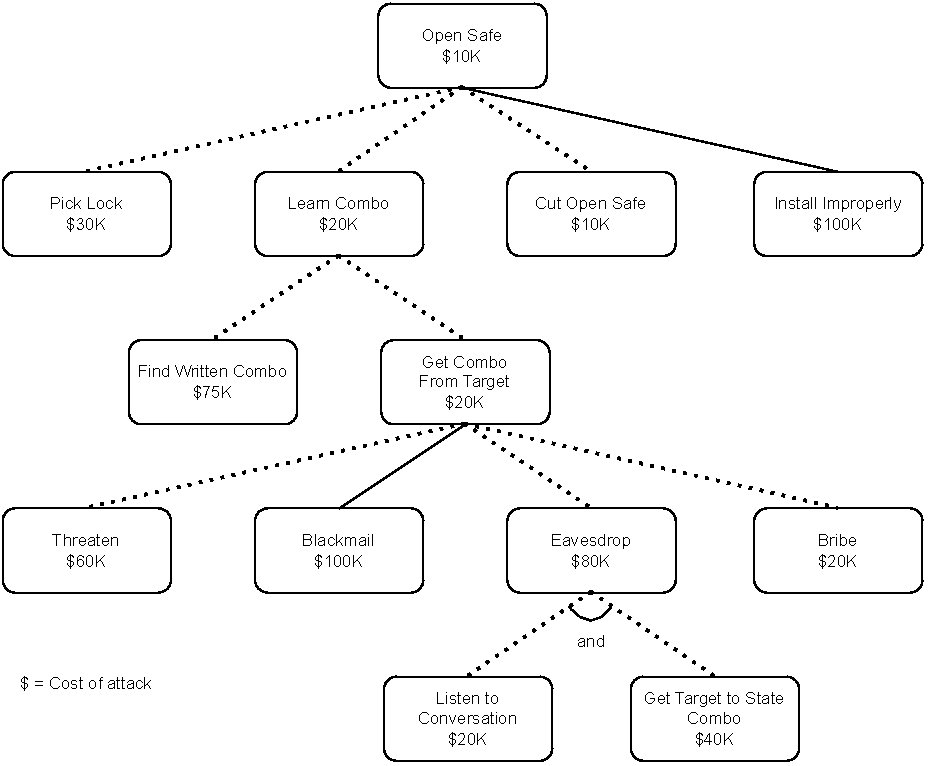
\includegraphics[width=0.8\linewidth]{figures/attack_graph.pdf}
  \caption[Illustration d'un graphe d'attaque décrivant un scénario de compromission d’un coffre-fort.]{Illustration d'un graphe d'attaque décrivant un scénario de compromission d’un coffre-fort. (adapté de \cite{schneier1999modeling})~: L’objectif racine \emph{Open Safe} est décomposé en quatre voies principales : \emph{Pick Lock} (\$30K), \emph{Learn Combo} (\$20K), \emph{Cut Open Safe} (\$10K) et \emph{Install Improperly} (\$100K). Par défaut, un nœud est de type \textsc{OU} (réaliser l’un des enfants suffit) ; lorsqu’un \emph{and} est indiqué, il s’agit d’un \textsc{ET} (tous les enfants sont requis). Les montants représentent des coûts estimés : pour un \textsc{OU}, le coût du parent est le \emph{minimum} des coûts enfants ; pour un \textsc{ET}, les coûts \emph{s’additionnent}.}
  \label{fig:attack_graphs}
\end{figure}

\

\noindent
\textbf{Arbres attaque-défense}~: \quad Les arbres attaque-défense~\cite{BKordy2010} (arbres \acparen{AD}) sont des modèles graphiques représentant les objectifs de l'attaquant et les contre-mesures du défenseur sous la forme d'une structure arborescente. Les arbres \acn{AD} fournissent une représentation plus abstraite du système et des objectifs des attaquants, tandis que les graphes d'attaque fournissent une représentation plus concrète des composants du système et de leurs relations. Un exemple d'arbre \acn{AD} est illustré en \autoref{fig:bank_attack_defense_tree}. La racine de l'arbre \acn{AD} représente l'objectif ultime des cyberattaquants. Les sous-nœuds associés aux branches représentent les différentes stratégies d'attaque que l'attaquant pourrait utiliser pour atteindre son objectif. Ils peuvent être accompagnés de contre-mesures préventives ou réactives du défenseur (pare-feu, systèmes de détection d'intrusion, plans d'intervention en cas d'incident, etc.).
Les arbres \acn{AD} permettent d'identifier les points faibles de la défense d'un système~\cite{BKordy2010}.

\begin{figure}[h!]
  \centering
  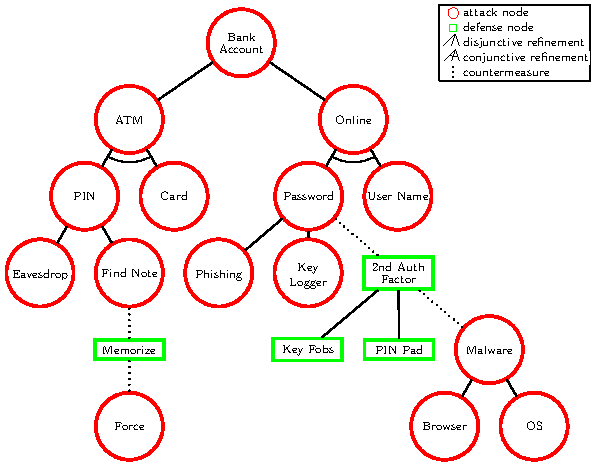
\includegraphics[width=\linewidth]{figures/adt.pdf}
  \caption[Illustration d'ADTree d'un scénario d'attaque sur un compte bancaire.]{Illustration d'ADTree décrivant un scénario d'attaque sur un compte bancaire. (tiré de \cite{BKordy2010})~: L'accès au compte peut être fait via un guichet automatique ou en ligne. Pour ce dernier cas, il est nécéssaire d'avoir un identifiant et un mot de passe obtenable par phishing ou un \textit{Key Logger}. Une contremesure à ces attaques est la double authentification construite avec une clé \textit{fob} ou un code pin.}
  \label{fig:bank_attack_defense_tree}
\end{figure}

\

\noindent
\textbf{Modélisation par réseaux de Petri}~: \quad Les réseaux de Petri pouvant être utilisés pour décrire des processus concurrents, certains travaux ont cherché à modéliser les attaquants et les défenseurs dans un système en réseau.
Les attaques extraites de bases de données peuvent être modélisées à l'aide de réseaux de Petri afin d'intégrer les cyberattaquants et les cyberdéfenseurs, leurs stratégies et le coût de leurs actions, comme dans ~\cite{MPetty2022}. Les réseaux de Petri se révèlent également utiles pour modéliser les attaques par injection de langage de requête structuré afin d'inclure les stratégies des joueurs~\cite{JBland2020}.
Ils sont utilisés comme cadre pour évaluer et comparer plusieurs modèles d'attaque.
Dans ~\cite{SYamaguchi2020}, le logiciel malveillant \textit{Mirai} a aussi été exprimé sous la forme d'un modèle formel avec des réseaux de Petri, permettant de simuler un combat entre un agent défenseur et \textit{Mirai}.

\

\noindent
\textbf{Modèles de jeu}~: \quad Certains travaux ont proposé de modéliser les interactions entre les attaquants et les défenseurs dans un réseau comme des joueurs dans un jeu, où chaque joueur dispose d'un ensemble d'actions qu'il peut effectuer.
Parmi les travaux notables, citons~: Panfili et al.~\cite{MPanfili2018}, où un jeu à somme générale multi-agents opposant un attaquant à un défenseur est utilisé pour trouver un compromis optimal entre les actions de prévention et les coûts~; Attiah et al.~\cite{AAttiah2018}, où un cadre théorique de jeu dynamique est proposé pour analyser les interactions entre l'attaquant et le défenseur comme un jeu de sécurité non coopératif~; et Xiaolin et al.~\cite{CXiaolin2008}, qui utilisent des modèles de processus de Markov pour évaluer les risques dans les systèmes en réseau.

\noindent
Certaines approches fondées sur la théorie des jeux s'inscrivent dans le cadre des \textquote{jeux stochastiques partiellement observables} (POSG) ou, plus précisément, dans celui des \textquote{processus de décision markoviens décentralisés partiellement observables} (Dec-POMDP). Les POSG et les Dec-POMDP sont tous deux des cadres de modélisation mathématique des problèmes de prise de décision dans lesquels des agents interagissent entre eux et dans un environnement stochastique~\cite{beynier2010}. Dans un POSG, un groupe d'agents interagit avec un environnement stochastique et partiellement observable. Chaque agent agit en fonction de ses propres observations et d'une politique locale. Les agents peuvent avoir des objectifs différents, car chaque agent a sa propre fonction de récompense et le jeu est généralement supposé être non coopératif~\cite{terry2020pettingzoo}. Dans un Dec-POMDP, plusieurs agents peuvent avoir une fonction de récompense commune et peuvent coordonner leurs actions pour atteindre un objectif commun, notamment en étant capables de communiquer~\cite{bernstein2013}.


\subsection{Les \textit{World Models} pour automatiser la modélisation en simulation}

En \acn{RL}, et en particulier en contexte d'observabilité partielle, les \textbf{modèles du monde}~\cite{ha2018recurrent, hafner2020dream} visent à apprendre des modèles internes approximant à la fois la dynamique de la fonction de transition et d'observation conjointement. Les \textit{World Models} permettent aux agents d'effectuer de la planification, d'améliorer l'efficacité échantillonnale, et de faciliter l'exploration sûre en permettant à l'agent de simuler des scénarios futurs. Cette approche appartient au paradigme du \acn{MBRL}~\cite{moerland2020model}, et se révèle particulièrement utile pour construire automatiquement des modèles de simulation à haute fidélité même en l'absence de représentation explicite de l'environnement.

Formellement, à chaque pas de temps $t$, on note $\omega_t \in \Omega$ l'observation courante, $a_t \in A$ l'action réalisée, et $\tilde{h}_{t-1} \in \mathcal{H}$ l'état caché récurrent résumant l'historique d'interaction jusqu'à $t-1$. Étant donné que les observations sont généralement de grande dimension (par exemple, des images ou des vecteurs d'état complexes), un encodeur $Enc: \Omega \rightarrow Z$ est appliqué pour projeter les observations dans un espace latent compact $Z$, avec $z_t = Enc(\omega_t)$, où $\dim(Z) \ll \dim(\Omega)$.

La structure temporelle principale est modélisée à l'aide d'un \textbf{Modèle Dynamique Latent Récurrent (\acparen{RLDM})}~\cite{hafner2020dream} $\mathcal{T}^{z} = f(g(h_{t-1}, z_t, a_t))$, qui prédit le prochain état latent $\hat{z}_{t+1}$ en mettant à jour l'état récurrent via $f$ et en appliquant une dynamique latente via $g$~:
\[
  h_t = f(h_{t-1}, z_t, a_t), \quad \hat{z}_{t+1} = g(h_t)
\]
où $f(\cdot)$ correspond typiquement à un réseau de neurones récurrent (par exemple un \acparen{LSTM}~\cite{hochreiter1997long}) appliqué à la concaténation de $h_{t-1}$, $z_t$ et $a_t$, et $g(\cdot)$ est une fonction (souvent implémentée par un \acparen{MLP}) mappant l'état récurrent vers la représentation latente de la prochaine observation.

L'état latent prédit est ensuite décodé par $Dec: Z \rightarrow \Omega$ pour produire l'observation prédite $\hat{\omega}_{t+1} = Dec(\hat{z}_{t+1})$. L'ensemble du modèle est entraîné conjointement pour minimiser à la fois la \emph{perte de reconstruction} $\|\omega_{t+1} - \hat{\omega}_{t+1}\|$ dans l'espace d'observation, et éventuellement une \emph{perte de prédiction latente} pour stabiliser l'apprentissage de la dynamique latente.

L'état caché récurrent $\tilde{h}_t$ joue le rôle d'un résumé compact de l'historique complet d'interaction jusqu'au temps $t$, évitant ainsi d'avoir à stocker explicitement de longues séquences observation-action.

Par souci de concision, nous définissons la composition complète qui associe directement observation courante, action et état récurrent à l'observation prédite suivante sous la forme du \textbf{Modèle de Prédiction d'Observation} (\acparen{OPM})~:
\[
  \mathcal{T}(h_{t-1}, \omega_t, a_t)~:= Dec(g(f(h_{t-1}, Enc(\omega_t), a_t))) = \hat{\omega}_{t+1}.
\]

\begin{figure}[h!]
  \centering
  \resizebox{\textwidth}{!}{%
    


\tikzset{every picture/.style={line width=0.75pt}} %set default line width to 0.75pt        

\begin{tikzpicture}[x=0.75pt,y=0.75pt,yscale=-1,xscale=1]
    %uncomment if require: \path (0,2102); %set diagram left start at 0, and has height of 2102

    %Straight Lines [id:da7945271061326031] 
    \draw    (100,1800) -- (111.5,1800) ;
    \draw [shift={(113.5,1800)}, rotate = 180] [color={rgb, 255:red, 0; green, 0; blue, 0 }  ][line width=0.75]    (6.56,-1.97) .. controls (4.17,-0.84) and (1.99,-0.18) .. (0,0) .. controls (1.99,0.18) and (4.17,0.84) .. (6.56,1.97)   ;
    %Straight Lines [id:da710289636295716] 
    \draw    (100,1835) -- (188,1834) -- (188,1820) ;
    \draw [shift={(188,1818)}, rotate = 90] [color={rgb, 255:red, 0; green, 0; blue, 0 }  ][line width=0.75]    (6.56,-1.97) .. controls (4.17,-0.84) and (1.99,-0.18) .. (0,0) .. controls (1.99,0.18) and (4.17,0.84) .. (6.56,1.97)   ;
    %Straight Lines [id:da9775676154282154] 
    \draw    (146.38,1800) -- (160,1800) ;
    \draw [shift={(162,1800)}, rotate = 180] [color={rgb, 255:red, 0; green, 0; blue, 0 }  ][line width=0.75]    (7.65,-2.3) .. controls (4.86,-0.97) and (2.31,-0.21) .. (0,0) .. controls (2.31,0.21) and (4.86,0.98) .. (7.65,2.3)   ;
    %Straight Lines [id:da789934339782699] 
    \draw    (100,1766) -- (122,1766) ;
    \draw [shift={(124,1766)}, rotate = 180] [color={rgb, 255:red, 0; green, 0; blue, 0 }  ][line width=0.75]    (6.56,-1.97) .. controls (4.17,-0.84) and (1.99,-0.18) .. (0,0) .. controls (1.99,0.18) and (4.17,0.84) .. (6.56,1.97)   ;
    %Shape: Trapezoid [id:dp2317709974845179] 
    \draw   (123.84,1754.74) -- (142.07,1760.21) -- (142.07,1771.42) -- (123.84,1776.88) -- cycle ;
    %Straight Lines [id:da7383754609221514] 
    \draw    (142,1766) -- (188,1766) -- (188,1780) ;
    \draw [shift={(188,1782)}, rotate = 270] [color={rgb, 255:red, 0; green, 0; blue, 0 }  ][line width=0.75]    (6.56,-1.97) .. controls (4.17,-0.84) and (1.99,-0.18) .. (0,0) .. controls (1.99,0.18) and (4.17,0.84) .. (6.56,1.97)   ;
    %Straight Lines [id:da49394763541143527] 
    \draw    (216,1800) -- (237.33,1799.94) ;
    \draw [shift={(239.33,1799.94)}, rotate = 179.85] [color={rgb, 255:red, 0; green, 0; blue, 0 }  ][line width=0.75]    (6.56,-1.97) .. controls (4.17,-0.84) and (1.99,-0.18) .. (0,0) .. controls (1.99,0.18) and (4.17,0.84) .. (6.56,1.97)   ;
    %Straight Lines [id:da8738633046359771] 
    \draw    (265.89,1800.03) -- (284.72,1800.03) ;
    \draw [shift={(286.72,1800.03)}, rotate = 180] [color={rgb, 255:red, 0; green, 0; blue, 0 }  ][line width=0.75]    (6.56,-1.97) .. controls (4.17,-0.84) and (1.99,-0.18) .. (0,0) .. controls (1.99,0.18) and (4.17,0.84) .. (6.56,1.97)   ;
    %Straight Lines [id:da3021616845453272] 
    \draw    (302,1800) -- (320.83,1800) ;
    \draw [shift={(322.83,1800)}, rotate = 180] [color={rgb, 255:red, 0; green, 0; blue, 0 }  ][line width=0.75]    (6.56,-1.97) .. controls (4.17,-0.84) and (1.99,-0.18) .. (0,0) .. controls (1.99,0.18) and (4.17,0.84) .. (6.56,1.97)   ;
    %Straight Lines [id:da8984410115217915] 
    \draw    (346,1800) -- (353.4,1800) -- (365.04,1800) ;
    \draw [shift={(367.04,1800)}, rotate = 180] [color={rgb, 255:red, 0; green, 0; blue, 0 }  ][line width=0.75]    (6.56,-1.97) .. controls (4.17,-0.84) and (1.99,-0.18) .. (0,0) .. controls (1.99,0.18) and (4.17,0.84) .. (6.56,1.97)   ;
    %Shape: Trapezoid [id:dp37639710819638017] 
    \draw   (423.61,1812) -- (405.38,1806.53) -- (405.38,1795.32) -- (423.61,1789.86) -- cycle ;
    %Straight Lines [id:da10289425963982124] 
    \draw    (384,1800) -- (403.04,1800) ;
    \draw [shift={(405.04,1800)}, rotate = 180] [color={rgb, 255:red, 0; green, 0; blue, 0 }  ][line width=0.75]    (6.56,-1.97) .. controls (4.17,-0.84) and (1.99,-0.18) .. (0,0) .. controls (1.99,0.18) and (4.17,0.84) .. (6.56,1.97)   ;
    %Straight Lines [id:da12692360321469986] 
    \draw    (424,1800) -- (443.04,1800) ;
    \draw [shift={(445.04,1800)}, rotate = 180] [color={rgb, 255:red, 0; green, 0; blue, 0 }  ][line width=0.75]    (6.56,-1.97) .. controls (4.17,-0.84) and (1.99,-0.18) .. (0,0) .. controls (1.99,0.18) and (4.17,0.84) .. (6.56,1.97)   ;
    %Shape: Trapezoid [id:dp27180057752038367] 
    \draw   (217.23,1670.74) -- (235.46,1676.21) -- (235.46,1687.42) -- (217.23,1692.88) -- cycle ;
    %Shape: Trapezoid [id:dp9437628483591106] 
    \draw   (309.61,1695) -- (291.38,1689.53) -- (291.38,1678.32) -- (309.61,1672.86) -- cycle ;
    %Straight Lines [id:da19635385567867214] 
    \draw    (310,1683) -- (328,1683) ;
    \draw [shift={(330,1683)}, rotate = 180] [color={rgb, 255:red, 0; green, 0; blue, 0 }  ][line width=0.75]    (6.56,-1.97) .. controls (4.17,-0.84) and (1.99,-0.18) .. (0,0) .. controls (1.99,0.18) and (4.17,0.84) .. (6.56,1.97)   ;
    %Straight Lines [id:da6136759960935583] 
    \draw    (196,1683) -- (214.83,1683) ;
    \draw [shift={(216.83,1683)}, rotate = 180] [color={rgb, 255:red, 0; green, 0; blue, 0 }  ][line width=0.75]    (6.56,-1.97) .. controls (4.17,-0.84) and (1.99,-0.18) .. (0,0) .. controls (1.99,0.18) and (4.17,0.84) .. (6.56,1.97)   ;
    %Straight Lines [id:da5198115307428596] 
    \draw    (236,1683) -- (255.04,1683) ;
    \draw [shift={(257.04,1683)}, rotate = 180] [color={rgb, 255:red, 0; green, 0; blue, 0 }  ][line width=0.75]    (6.56,-1.97) .. controls (4.17,-0.84) and (1.99,-0.18) .. (0,0) .. controls (1.99,0.18) and (4.17,0.84) .. (6.56,1.97)   ;
    %Straight Lines [id:da6362560665768464] 
    \draw    (270,1683) -- (289.04,1683) ;
    \draw [shift={(291.04,1683)}, rotate = 180] [color={rgb, 255:red, 0; green, 0; blue, 0 }  ][line width=0.75]    (6.56,-1.97) .. controls (4.17,-0.84) and (1.99,-0.18) .. (0,0) .. controls (1.99,0.18) and (4.17,0.84) .. (6.56,1.97)   ;
    %Shape: Rectangle [id:dp3864765488610862] 
    \draw  [color={rgb, 255:red, 74; green, 144; blue, 226 }  ,draw opacity=1 ][dash pattern={on 0.84pt off 2.51pt}] (70,1720) -- (475,1720) -- (475,1855) -- (70,1855) -- cycle ;
    %Shape: Rectangle [id:dp17767261593347572] 
    \draw  [color={rgb, 255:red, 65; green, 117; blue, 5 }  ,draw opacity=1 ][dash pattern={on 0.84pt off 2.51pt}] (175,1660) -- (355,1660) -- (355,1700) -- (175,1700) -- cycle ;
    %Shape: Polygon [id:ds8294746409292746] 
    \draw  [color={rgb, 255:red, 208; green, 2; blue, 27 }  ,draw opacity=1 ][dash pattern={on 0.84pt off 2.51pt}] (390,1845) -- (75,1845) -- (75,1780.92) -- (150,1780) -- (150,1750) -- (390,1750) -- cycle ;


    % Text Node
    \draw (333.5,1764.5) node  [color={rgb, 255:red, 208; green, 2; blue, 27 }  ,opacity=1 ] [align=left] {\footnotesize \textbf{\textit{RDLM}}};
    % Text Node
    \draw (317.5,1734.5) node  [color={rgb, 255:red, 74; green, 144; blue, 226 }  ,opacity=1 ] [align=left] {\footnotesize Modèle de prédiction d'observation (\textbf{\textit{OPM}})};
    % Text Node
    \draw (264.5,1645.5) node  [color={rgb, 255:red, 65; green, 117; blue, 5 }  ,opacity=1 ] [align=left] {{\footnotesize \textbf{Auto-encodeur}}};
    % Text Node
    \draw (189.5,1683) node  [font=\tiny] [align=left] {$\displaystyle \omega _{t}$};
    % Text Node
    \draw (340,1682) node  [font=\tiny] [align=left] {$\displaystyle \hat{\omega }_{t}$};
    % Text Node
    \draw (301.5,1679.5) node   [align=left] {{\tiny Dec}};
    % Text Node
    \draw (225.38,1676.5) node   [align=left] {{\tiny Enc}};
    % Text Node
    \draw (264.5,1684) node  [font=\tiny] [align=left] {$\displaystyle z_{t}$};
    % Text Node
    \draw (456.54,1799) node  [font=\tiny] [align=left] {$\displaystyle \hat{\omega }_{t+1}$};
    % Text Node
    \draw (415.5,1796.5) node   [align=left] {{\tiny Dec}};
    % Text Node
    \draw (375.5,1799) node  [font=\tiny] [align=left] {$\displaystyle z_{t+1}$};
    % Text Node
    \draw (132,1760.5) node   [align=left] {{\tiny Enc}};
    % Text Node
    \draw (295,1798) node  [font=\tiny] [align=left] {$\displaystyle \tilde{h}_{t}$};
    % Text Node
    \draw    (239.48,1779) -- (265.48,1779) -- (265.48,1817) -- (239.48,1817) -- cycle  ;
    \draw (252.48,1798) node  [font=\tiny] [align=left] {\begin{minipage}[lt]{14.99pt}\setlength\topsep{0pt}
            \begin{center}
                \phantom{X}\\\textit{RNN}
            \end{center}

        \end{minipage}};
    % Text Node
    \draw  [color={rgb, 255:red, 255; green, 255; blue, 255 }  ,draw opacity=1 ][fill={rgb, 255:red, 255; green, 255; blue, 255 }  ,fill opacity=1 ]  (157.5,1757) -- (174.5,1757) -- (174.5,1773) -- (157.5,1773) -- cycle  ;
    \draw (166,1765) node  [font=\tiny] [align=left] {$\displaystyle z_{t}$};
    % Text Node
    \draw    (162,1782) -- (216,1782) -- (216,1818) -- (162,1818) -- cycle  ;
    \draw (189,1800) node  [font=\tiny] [align=left] {\begin{minipage}[lt]{34pt}\setlength\topsep{0pt}
            \begin{center}
                \phantom{X}\\\textit{concatenate}
            \end{center}

        \end{minipage}};
    % Text Node
    \draw (91,1833) node  [font=\tiny] [align=left] {$\displaystyle \tilde{h}_{t-1}$};
    % Text Node
    \draw (91.5,1801) node  [font=\tiny] [align=left] {$\displaystyle a_{t}$};
    % Text Node
    \draw (91.5,1766) node  [font=\tiny] [align=left] {$\displaystyle \omega _{t}$};
    % Text Node
    \draw    (322.5,1792) -- (345.5,1792) -- (345.5,1807) -- (322.5,1807) -- cycle  ;
    \draw (334,1799.5) node  [font=\tiny] [align=left] {MLP};
    % Text Node
    \draw    (113,1788) -- (146,1788) -- (146,1813) -- (113,1813) -- cycle  ;
    \draw (129.5,1800.5) node  [font=\tiny] [align=left] {one-hot\\encode};


\end{tikzpicture}
  }
  \caption{Illustration de l'architecture d'un World Model comprenant l'Auto-encodeur et l'OPM}
  \label{fig:single_agent_world_model}
\end{figure}

La \autoref{fig:single_agent_world_model} illustre l'architecture d'un World Model comprenant l'Auto-encodeur et l'\acn{OPM}.

\textbf{Phase d'entraînement de l'auto-encodeur :} Un auto-encodeur est d'abord entraîné à encoder et décoder les observations en représentations latentes. L'objectif est de minimiser l'écart entre les observations réelles et les observations décodées.

\textbf{Initialisation et traitement des transitions :} Initialement, l'état caché récurrent $\tilde{h}_{t-1}$ est initialisé au vecteur nul. Pour chaque historique et chaque transition, un vecteur d'entrée est construit en concaténant trois éléments : la représentation de l'observation $z_t$, l'action $a_t$ (après encodage one-hot) et l'état caché récurrent $\tilde{h}_{t-1}$.

\textbf{Fonctionnement du \acn{RLDM} :} Ce vecteur d'entrée est traité par le \acn{RLDM} selon un processus en deux étapes. D'abord, il passe par le \acn{RNN} qui met à jour l'état caché récurrent avec les nouvelles transitions pour obtenir $\hat{h}_t$. Ensuite, ce vecteur est transmis à un \acn{MLP} qui détermine la représentation latente de l'observation suivante $\hat{z}_{t+1}$.

\textbf{Entraînement et prédiction :} Le \acn{RLDM} est entraîné à minimiser l'erreur quadratique entre l'observation prédite et l'observation réelle. Une fois l'entraînement terminé, une représentation latente d'observation prédite peut être décodée en une observation prédite $\omega_{t+1}$.

\chapter{Les verrous d'une méthode de conception}
\label{chap:verrous}

\noindent
Le chapitre précédent a introduit les concepts fondamentaux nécessaires à la compréhension de notre démarche, en s'appuyant sur trois piliers théoriques~: l'organisation explicite des \acn{SMA} à travers des modèles comme \textit{$\mathcal{M}OISE^+$}, \acn{MARL}, et les techniques de modélisation d'environnement via les \textit{World Models} notamment. Ces notions constituent l'ossature sur laquelle repose notre méthode de conception.

Toutefois, ces cadres théoriques, pris isolément, ne permettent pas de répondre aux exigences posées par la thèse dans le \autoref{chap:verrous}. En particulier, la conception automatique d'un \acn{SMA} adapté à un environnement cible reste limitée par plusieurs obstacles théoriques ou technologiques, que nous identifions ici comme des \textit{verrous scientifiques}.

Ce chapitre a pour objectif d'analyser, pour chacune des hypothèses H1 à H4 formulées précédemment, l'état de l'art pertinent, les manques ou limites existants, ainsi que les verrous associés. Il s'agit ainsi d'établir une cartographie critique des défis que notre méthode devra relever, tout en préparant les fondations conceptuelles de la \autoref{part:methode}, où nous présentons notre réponse méthodologique sous la forme de la méthode \acn{MAMAD}.


\section{Les Worlds Models pour simuler des environnement multi-agents}

\noindent
Les travaux présentés dans le \autoref{chap:concepts} ont montré l'intérêt de disposer d'un environnement simulé pour entraîner des agents de manière sûre, rapide et contrôlée. Dans cette perspective, les \textit{World Models} constituent une approche prometteuse, permettant d'apprendre une dynamique approximative de l'environnement à partir de données collectées. Ces modèles sont largement utilisés en apprentissage par renforcement, notamment dans des contextes mono-agent, mais restent sous-explorés en environnement multi-agent complexe.

\medskip

\noindent
La littérature récente montre un regain d'intérêt pour l'automatisation de la conception de \acn{SMA}, notamment via l'ingénierie dirigée par les modèles, les frameworks organisationnels paramétrables, ou encore les générateurs de code à partir de spécifications. Des travaux comme INGENIAS~\cite{Pavon2003}, KB-ORG~\cite{Sims2008} ou AutoGenesisAgent~\cite{harper2024autogenesisagent} visent à automatiser la génération d'architectures agents à partir de modèles symboliques. Néanmoins, ces approches supposent en général un environnement connu, structuré, voire entièrement spécifié a priori.

\noindent
Dans le domaine de l'apprentissage, des travaux récents en cybersécurité~\cite{hammar2023scalable} ont exploré la génération automatique de scénarios pour entraîner des agents en simulation. Ces environnements, bien que plus dynamiques, sont encore conçus manuellement ou via des générateurs à base de règles, et ne s'adaptent pas aux interactions des agents. À ce jour, aucun pipeline complet ne relie la collecte de données dans un environnement réel à l'entraînement de politiques multi-agents via un modèle simulé appris de manière autonome.

\medskip

\noindent
Le cadre des World Models~\cite{Ha2018} propose une solution intéressante à ce besoin. En apprenant une représentation latente compressée de l'environnement et sa dynamique, il devient possible de simuler des trajectoires cohérentes pour entraîner des politiques sans interaction réelle. Toutefois, ces approches ont été principalement développées pour des environnements mono-agents à observation complète.

\noindent
Appliquer les \textit{World Models} à des environnements multi-agents soulève plusieurs défis~:
\begin{itemize}
  \item \textbf{Représentation conjointe}~: comment encoder et combiner des observations partielles issues de plusieurs agents hétérogènes~;
  \item \textbf{Dynamique coordonnée}~: comment apprendre une transition qui tient compte des effets d'interaction ou de coopération~;
  \item \textbf{Évolutivité}~: comment maintenir la qualité de la simulation lorsque le nombre d'agents et d'actions augmente.
\end{itemize}

\noindent
À notre connaissance, aucune approche ne propose actuellement un \textit{World Model} multi-agent générique capable de simuler des environnements partiellement observables avec des interactions complexes entre agents. Cela constitue un verrou méthodologique majeur à l'automatisation de la conception de \acn{SMA}~: sans modèle simulé réaliste, il est difficile de guider ou d'évaluer l'apprentissage des politiques à grande échelle.

\medskip

\noindent
\textbf{Hypothèse H2~:} il est possible d'apprendre automatiquement un modèle simulé multi-agent (World Model) à partir de trajectoires collectées dans un environnement cible, en combinant des représentations latentes et des prédictions conjointes adaptées à l'apprentissage multi-agent.


\section{L'intégration de contraintes/guidages organisationnelles dans le processus MARL}

\noindent
Le \acn{MARL}, tel que présenté dans le \autoref{chap:concepts}, permet aux agents de développer de manière autonome des politiques coopératives dans des environnements complexes et dynamiques. Toutefois, la nature exploratoire du \acn{MARL} rend difficile le contrôle précis des comportements émergents, en particulier lorsque des exigences critiques de sûreté, de coordination ou de structure doivent être respectées.

\medskip

\noindent
Les travaux en \textit{Safe Reinforcement Learning} ont cherché à intégrer des contraintes dans le processus d'apprentissage afin d'éviter certains comportements indésirables. Par exemple, \acn{CPO}~\cite{achiam2017constrained} garantit que la politique reste proche d'un ensemble d'actions autorisées, tandis que \textit{Deep Constrained Q-Learning}~\cite{kalweit2020deep} applique des contraintes explicites sur la mise à jour des valeurs Q. D'autres approches introduisent des mécanismes de \textit{shielding}, \textit{reward shaping} ou encore l'intégration de retours humains (cf.~\cite{zhou2025mentor}). Ces travaux montrent qu'il est possible d'influencer l'apprentissage en encadrant l'espace des politiques, tout en maintenant une capacité d'adaptation.

\noindent
Cependant, la majorité de ces méthodes opèrent à un niveau \textit{comportemental} local~: elles imposent des règles sur les actions possibles, ou ajustent la récompense pour favoriser certaines trajectoires. Très peu de travaux intègrent des contraintes \textit{organisationnelles} symboliques, c'est-à-dire des spécifications abstraites sur les rôles, missions ou interactions attendues entre agents.

\medskip

\noindent
La littérature sur le \acn{MARL} s'est principalement concentrée sur l'optimisation de la coopération entre agents dans des environnements incertains et partiellement observables~\cite{Zhang2021, Papoudakis2021}. Toutefois, les approches classiques négligent généralement l'incorporation de contraintes symboliques ou organisationnelles dans le processus d'apprentissage. Les agents apprennent par essais-erreurs sans garantie que leurs comportements émergents respecteront des exigences de conception critiques, comme des règles de sûreté, le respect des rôles, ou des hiérarchies d'équipe.

\noindent
Plusieurs travaux récents ont tenté de combler cette lacune via des techniques d'apprentissage par renforcement sensibles aux contraintes. \textit{Constraint-Guided Reinforcement Learning}~\cite{spieker2021constraint} intègre des modèles de contraintes explicites dans l'interaction agent-environnement, permettant d'apprendre des politiques respectant des bornes comportementales prédéfinies. \textit{Deep Constrained Q-Learning}~\cite{kalweit2020deep} impose des contraintes à court et moyen terme dans la mise à jour des valeurs Q, assurant ainsi le respect de critères de performance et de sécurité. L'approche \acn{CPO}~\cite{achiam2017constrained} offre des garanties théoriques de satisfaction des contraintes durant la recherche de politiques, et \textit{MENTOR}~\cite{zhou2025mentor} guide les agents dans un cadre hiérarchique à l'aide de retours humains et de sous-objectifs dynamiquement contraints. Enfin, l'apprentissage contraint sans fonction de récompense explicite~\cite{miryoosefi2022} optimise directement la satisfaction de contraintes en contournant l'ingénierie de récompenses.

\medskip

\noindent
Si ces approches renforcent le contrôle des politiques apprises, elles restent limitées à un niveau local ou comportemental et n'intègrent pas des modèles de conception symboliques tels que ceux développés en ingénierie des \acn{SMA}.

\medskip

\noindent
Les modèles issus de l'ingénierie des \acn{SMA}, comme \textit{$\mathcal{M}OISE^+$}~\cite{hubner2002moise}, proposent au contraire une structuration explicite du système via des rôles, des missions à accomplir, et des groupes formés dynamiquement. À notre connaissance, aucune approche ne permet de guider ou contraindre les agents à s'aligner sur des comportements d'agents évoluant dans une organisation structurée et fonctionnelle telle que proposée dans $\mathcal{M}OISE^+$.


%ttt

\medskip

\noindent
Ainsi, un verrou fondamental demeure~: il n'existe pas de méthode permettant de structurer et de guider l'apprentissage \acn{MARL} à partir de spécifications organisationnelles riches, telles que celles proposées par $\mathcal{M}OISE^+$, tout en assurant un compromis entre autonomie d'apprentissage et respect de contraintes. Or, dans des domaines critiques (cyberdéfense, secours, coordination robotique), ce besoin est central.

\medskip

\noindent
\textbf{Hypothèse H3~:} il est possible de contraindre ou guider l'apprentissage multi-agent en intégrant des spécifications organisationnelles (rôles, missions, groupes) sous forme de contraintes explicites, afin de produire des politiques sûres, coordonnées et explicables, sans restreindre excessivement la capacité d'apprentissage des agents.


\section{L'extraction automatisée des spécifications organisationnelles émergentes}

Alors que la tradition \acn{AOSE} garantit l'explicabilité à travers des artefacts de conception structurés (tels que des protocoles, des rôles, des missions ou des objectifs), ces éléments symboliques sont généralement perdus dans les approches classiques du \acn{MARL}. Les politiques apprises sont souvent représentées sous la forme de réseaux de neurones opaques, rendant difficile l'évaluation de la conformité des comportements des agents avec l'intention de conception initiale ou les principes organisationnels. Bien que l'explicabilité en \acn{MARL} ait suscité un intérêt croissant, la majorité des travaux existants se concentrent sur le comportement individuel des agents ou les mécanismes internes des politiques, sans aborder leur alignement collectif ou organisationnel.

Un nombre croissant de recherches cherche à améliorer l'interprétabilité via la conception de modèles ou l'analyse post-hoc. Zabounidis et al.~\cite{zabounidis2023concept} intègrent des concepts interprétables dans la boucle d'apprentissage, en forçant les agents à prédire des concepts compréhensibles par un humain avant d'agir. Cela favorise la transparence et permet des corrections par des experts. Iturria-Rivera et al.~\cite{iturria2024explainable} utilisent la décomposition de la récompense dans les fonctions de valeur factorisées (par exemple VDN, QMIX) pour exposer la contriobjectifion de chaque composante aux décisions de l'agent. Liu et al.~\cite{liu2025} proposent MIXRTs, une architecture hybride combinant réseaux neuronaux récurrents et arbres de décision pour l'apprentissage de politiques interprétables. D'autres efforts comme ceux de Poupart et al.~\cite{poupart2025perspectives} introduisent des méthodes post-hoc telles que la rétropropagation de la pertinence (relevance backpropagation) ou le patching d'activations. Li et al.~\cite{li2025from} emploient des approximations basées sur la valeur de Shapley pour transformer des politiques de type deep \acn{RL} en structures interprétables.

Cependant, ces approches restent principalement limitées à des analyses locales ou centrées sur un seul agent. Elles ne permettent pas d'interpréter le comportement collectif d'un \acn{SMA} ni de relier ces dynamiques à des structures organisationnelles symboliques. Très peu d'études abordent explicitement la possibilité d'inférer des rôles, objectifs ou structures émergentes à partir de trajectoires observées.

Certains travaux connexes offrent néanmoins des pistes intéressantes. Berenji et Vengerov~\cite{berenji2000learning} modélisent les dépendances entre agents dans des missions de drones afin d'améliorer leur coordination, et Yusuf et Baber~\cite{yusuf2020inferential} proposent un raisonnement bayésien pour soutenir une coordination dynamique. Bien que ces contriobjectifions soulignent l'intérêt d'une modélisation symbolique à partir de comportements, elles ne fournissent pas de mécanismes pour inférer explicitement des rôles ou objectifs organisationnels à partir des trajectoires. De leur côté, Serrino et al.~\cite{serrino2019finding} analysent les interactions sociales pour identifier des rôles émergents, mais leur approche reste centrée sur des dynamiques sociales informelles sans formalisation organisationnelle.

En résumé, aucune méthode existante ne permet actuellement d'extraire automatiquement des spécifications organisationnelles (telles que des structures de rôles, des missions ou des objectifs collectifs) à partir de trajectoires d'agents entraînés. Or, une telle capacité permettrait de combler le fossé entre les approches symboliques prescriptives de l'\acn{AOSE} et les approches apprenantes fondées sur l'émergence. Elle offrirait un cadre pour évaluer l'organisation implicite d'un \acn{SMA}, identifier des écarts avec un modèle attendu, et potentiellement réinjecter ces connaissances dans une boucle de conception organisationnelle itérative. Cette hypothèse ouvre la voie à une nouvelle génération de méthodes de diagnostic, de rétro-ingénierie et d'adaptation des \acn{SMA} entraînés par apprentissage.

\medskip

\noindent
\textbf{Hypothèse H4~:} il est possible d'inférer automatiquement des spécifications organisationnelles émergentes à partir des trajectoires d'agents entraînés, en combinant des techniques d'analyse symbolique, de clustering comportemental et de projection organisationnelle, afin d'évaluer et d'adapter l'organisation d'un \acn{SMA} de manière itérative.


\section{Un cadre Markovien pour formaliser le problème de conception et sa résolution en MARL}

\noindent
La conception d'un \acn{SMA} implique généralement de définir des rôles, des interactions et des règles de coordination dans un environnement donné. Traditionnellement, cette activité repose sur une modélisation symbolique, où les concepteurs spécifient manuellement les comportements et les structures attendus. À l'inverse, les approches fondées sur l'apprentissage, notamment le \acn{MARL}, cherchent à découvrir ces comportements de manière automatique à partir d'expériences. Il devient alors essentiel de disposer d'un cadre formel permettant de représenter le problème de conception lui-même comme un problème de décision, résoluble par apprentissage.

\medskip

\noindent
Les travaux en \acn{MARL} se basent généralement sur des modèles Markoviens multi-agents, tels que les \acn{Dec-MDP} ou les \acn{Dec-POMDP}. Dans un \acn{Dec-POMDP}, chaque agent dispose d'observations partielles, d'une politique locale, et d'une fonction de récompense partagée ou individuelle. Ce formalisme permet de représenter des dynamiques complexes, distribuées et incertaines, tout en tenant compte de la coordination nécessaire entre agents.

\noindent
Cependant, dans la majorité des cas, ces modèles sont utilisés pour représenter des problèmes d'exécution (ex.~: résolution de tâches) plutôt que des problèmes de conception. Le lien entre spécifications organisationnelles ($\mathcal{M}OISE^+$, rôles, missions) et les composantes du \acn{Dec-POMDP} n'est généralement pas formalisé. De plus, ces modèles ne permettent pas directement d'imposer des contraintes symboliques sur les politiques ou les trajectoires.

\medskip

\noindent
Pour pallier cette limite, plusieurs extensions des \acn{MDP}s ont été proposées~:
\begin{itemize}
  \item les \textit{Constrained \acn{MDP}} (CMDP), où certaines contraintes (coût, sécurité) doivent être respectées au cours de l'exécution~;
  \item les \textit{Constrained \acn{Dec-POMDP}}, qui introduisent des contraintes globales ou locales sur les politiques des agents~;
  \item les formulations basées sur des \textit{specifications logiques} pour encadrer l'espace des politiques admissibles.
\end{itemize}

\noindent
Ces modèles constituent des bases intéressantes, mais restent rarement utilisés pour formaliser le processus même de \textit{conception} d'un \acn{SMA}. En effet, ils supposent généralement que la dynamique de l'environnement est connue, que l'espace d'état est spécifié, et que les contraintes sont codées à bas niveau. Il manque donc un cadre unifié permettant de représenter~:
\begin{itemize}
  \item les dynamiques simulées de l'environnement (World Model)~;
  \item les contraintes organisationnelles ($\mathcal{M}OISE^+$)~;
  \item et la recherche de politiques collectives compatibles avec ces éléments.
\end{itemize}

\medskip

\noindent
Nous proposons d'enrichir le \acn{Dec-POMDP} en y injectant deux structures complémentaires~:
\begin{enumerate}
  \item une fonction d'environnement $\mathcal{T}$, apprise à partir de données (World Model)~;
  \item un ensemble de contraintes organisationnelles symboliques, représentées sous forme de relations $(h, o) \mapsto A_{autorisé}$ ou de fonctions de récompense de trajectoire.
\end{enumerate}

\noindent
L'idée est de voir la conception d'un \acn{SMA} comme un \textit{problème d'optimisation sous contraintes}, où les politiques sont apprises pour maximiser une récompense tout en respectant des contraintes structurelles, organisationnelles ou comportementales. Cette formalisation ouvre la voie à un apprentissage dirigé et sécurisé des comportements.

\medskip

\noindent
\textbf{Hypothèse H1~:} il est possible de formaliser le problème de conception d'un \acn{SMA} comme un problème d'optimisation dans un cadre \acn{Dec-POMDP} enrichi, en y intégrant à la fois un modèle simulé de l'environnement (World Model) et des contraintes organisationnelles dérivées d'un modèle comme $\mathcal{M}OISE^+$.

\section*{Synthèse des verrous identifiés}

\noindent
Ce chapitre a permis d'établir un lien entre les hypothèses de recherche formulées en \autoref{part:contexte}, l'état de l'art dans les domaines concernés, et les verrous scientifiques empêchant aujourd'hui une conception automatisée, sûre et explicable des systèmes multi-agents.

\medskip

\noindent
Le \autoref{tab:verrous_hypotheses} synthétise cette analyse. Il met en évidence que, malgré des avancées importantes dans des domaines comme le \acn{MARL}, la simulation via World Models, l'apprentissage contraint, ou l'explicabilité, aucun cadre existant ne permet aujourd'hui de traiter conjointement~:
\begin{itemize}
  \item la modélisation dynamique d'un environnement inconnu (H2)~;
  \item l'apprentissage multi-agent sous contraintes structurelles (H3)~;
  \item l'analyse organisationnelle des comportements appris (H4)~;
  \item et la formalisation complète de ce processus dans un cadre décisionnel résoluble (H1).
\end{itemize}

\noindent
Ces lacunes justifient la nécessité d'une approche intégrée, qui articule apprentissage, organisation et analyse dans une boucle de conception fermée. Les hypothèses H1 à H4 révèlent ainsi quatre besoins méthodologiques complémentaires, qui seront pris en charge dans notre proposition.

\medskip

\noindent
La partie suivante introduit la méthode \textbf{\acn{MAMAD}} (\acparen{SMA}), développée précisément pour répondre à ces besoins. Cette méthode repose sur une formalisation unifiée du processus de conception comme un problème d'optimisation organisationnelle sous contraintes, résolu par apprentissage, simulé via un World Model, et analysé en retour pour guider les itérations futures.


\begin{table}[H]
  \centering
  \caption{Synthèse des travaux prometteurs, verrous, limites et besoins méthodologiques par hypothèse}
  \label{tab:synthese_hypotheses}
  \renewcommand{\arraystretch}{1.2}
  {%
    \footnotesize
    \begin{tabularx}{\textwidth}{cXXXX}
      \hline
      \textbf{Hyp.}
       & \textbf{Travaux prometteurs}
       & \textbf{Verrous principaux}
       & \textbf{Limites des travaux existants}
       & \textbf{Besoins méthodologiques}                                                                                                                                                                      \\
      \hline

      \textbf{H-MOD}
       & Dec-POMDP comme cadre adaptable ; World Models pour la modélisation automatique
       & Lourdeur de la modélisation manuelle ; absence de bibliothèques spécialisées cyber ; extension multi-agent des World Models non résolue
       & World Models limités au mono-agent ou à des contextes simples ; peu d'approches exploitant des observations distribuées ; modèles markoviens trop simples pour aider à la modélisation manuelle
       & Apprendre un World Model multi-agent structuré autour de représentations latentes ; proposer un modèle markovien utilisable pour modéliser un environnement de cyberdéfense                           \\
      \hdashline

      \textbf{H-TRN}
       & Safe RL (CPO, DCQL) ; Constraint-Guided RL ; intégration potentielle de modèles organisationnels (MOISE+)
       & Faible expressivité organisationnelle des méthodes existantes ; absence de cadre unifié entre organisation symbolique et MARL ; manque de garanties globales
       & Constrained RL ne prend pas en compte les structures organisationnelles ; intégration de spécifications symboliques limitée à l'exécution
       & Introduire des contraintes symboliques dans le processus MARL pour guider l'apprentissage et filtrer les actions                                                                                      \\
      \hdashline

      \textbf{H-ANL}
       & MAVIPER et modèles interprétables ; clustering de trajectoires pour inférence de rôles ; ROMA
       & Absence de lien avec modèles symboliques ; manque d'automatisation ; pas de cadre d'évaluation de l'explicabilité organisationnelle
       & Explicabilité surtout locale (niveau agent/action) ; peu de travaux inférant des rôles, missions ou objectifs collectifs
       & Inférer automatiquement rôles, missions et objectifs à partir de trajectoires ; proposer un cadre théorique pour l'explicabilité organisationnelle                                                    \\
      \hdashline

      \textbf{H-TRF}
       & Domain adaptation / Sim2Real ; Robust RL ; Online calibration (PILCO)
       & Approches partielles (transfert ou recalibrage, mais pas les deux) ; absence de cadre intégré de jumeau numérique adaptatif et de mise à jour conjointe des politiques
       & Domain adaptation et sim2real se concentrent sur le transfert initial sans recalibrage dynamique ; robust RL ne met pas à jour le modèle simulé ; calibration en ligne sans adaptation des politiques
       & Développer un framework unificateur de jumeau numérique couplant mise à jour continue du modèle simulé et adaptation conjointe des politiques multi-agents                                            \\
      \hline
    \end{tabularx}
  }
\end{table}


\clearpage
\thispagestyle{empty}
\null
\newpage

\chapter*{Conclusion}
\addcontentsline{toc}{chapter}{\textbf{Conclusion}}

\noindent
Cette deuxième partie a posé les fondations théoriques et critiques nécessaires à l'élaboration de notre méthode de conception. En s'appuyant sur les enjeux identifiés dans la \autoref{part:contexte}, elle a permis de clarifier les concepts mobilisés, d'identifier les manques persistants dans la littérature, et de formuler les verrous qui justifient la nécessité d'une nouvelle approche.

\medskip

\noindent
Le \autoref{chap:concepts} a introduit les trois piliers conceptuels sur lesquels s'appuie notre démarche~: (1) les modèles organisationnels, en particulier \textit{$\mathcal{M}OISE^+$}, qui offrent une structuration explicite du \acn{SMA}~; (2) Le \acn{MARL}, qui permet une acquisition autonome de politiques dans des environnements complexes~; et (3) les \textit{World Models}, qui fournissent un moyen de simuler un environnement à partir de données, ouvrant la voie à une exploration sécurisée et accélérée.

\noindent
Le \autoref{chap:verrous} a prolongé cette analyse en examinant les limites de l'état de l'art face aux exigences soulevées par notre question. Chaque hypothèse de recherche (H1 à H4) a été replacée dans son contexte scientifique, discutée à la lumière des travaux existants, et reliée à un verrou spécifique~:
\begin{itemize}
  \item la difficulté à représenter le problème de conception dans un cadre décisionnel formel (H1)~;
  \item l'absence de \textit{World Models} adaptés au contexte multi-agent (H2)~;
  \item le manque d'intégration de contraintes organisationnelles dans l'apprentissage (H3)~;
  \item l'impossibilité d'analyser les comportements appris à l'échelle organisationnelle (H4).
\end{itemize}

\medskip

\noindent
Ces constats convergent vers un besoin commun~: celui d'une méthode unifiée, capable d'orchestrer l'ensemble du processus de conception (de la modélisation de l'environnement à l'analyse des comportements) en intégrant apprentissage et organisation dans une boucle cohérente. C'est précisément l'objectif de la méthode \acn{MAMAD}, que nous introduisons dans la partie suivante.

\noindent
La \autoref{part:methode} présente cette méthode en détail. Elle repose sur une formalisation du problème de conception comme un \acn{Dec-POMDP} contraint enrichi par des structures organisationnelles. \acn{MAMAD} articule quatre étapes principales (modélisation, apprentissage, analyse et transfert) pour automatiser, structurer et affiner la conception des \acn{SMA} dans des environnements dynamiques et incertains.

\clearpage
\thispagestyle{empty}
\null
\newpage

\cleardoublepage
\phantomsection
% \pdfbookmark[1]{La méthode MAMAD}{La méthode MAMAD}
\markboth{\spacedlowsmallcaps{La méthode MAMAD}}{\spacedlowsmallcaps{La méthode MAMAD}}
\part{La méthode MAMAD}
\label{part:methode}

\clearpage
\thispagestyle{empty}
\null
\newpage

% todo : Initialement, dans la partie I, notre problème était un problème de conception logiciel d'un \acn{SMA} de Cyberdéfense capable d'assurer la Cyberdéfense de façon optimale compte tenu des contraintes dynamique de l'environnement et des concepteur. Nous avons formalisé le fait que pour répondre à cette question de recherche globale, il faut répondre simultanément à 6 critères (Autonomie - C1, Performance - C2, Adaptation - C3, Contrôle - C4, Explicabilité - C5, Robustesse - C6). Nous avons donc poursuivi une première revue de littérature qui nous a permis de comprendre qu'assez peu de travaux s’intéressent à une approche multi-agent pour la Cyberdéfense et que les travaux qui couvrent le plus de critères sont à chercher du côté de l'approche connexioniste qui favorise la performance et l'adaptation là où l'approche purement symbolique favorise l'explicabilité et le controle. Fort de ce constat, nous avons proposé de voir la question de recherche globale au travers le prisme d'un problème d'optimisation sous contraintes où la politique conjointe est à optimiser pour maximiser une récompense qui encode le succès dans l'atteinte d'un objectif de Cyberdéfense (ou un conglomérat d'objectifs) et où les contraintes sont formalisées comme des spécifications organisationnelles. A partir de cette formalisation, la complexité de la question de recherche globale apparait abordable au travers de 4 activités : Modélisation, Entrainement, Analyse et Transfert. On sait pour chaque activité les données en entrée, les données en sortie attendues et donc aussi les objectifs de chaque activité.
% A partir de cette vision, la partie \acn{II} présente les travaux qui couvrent les objectifs pour chaque activité, permettant ainsi de savoir quels sont les domaines/sous-domaines ou travaux qui semble le plus adaptés (ou qui nécéssitent le moins de contributions supplémentaires) pour atteindre les objectifs de chaque activités. Compte tenu des travaux identifiés comme les plus prometteurs, on en déduit donc les verrous qui restent encore à combler par de nouvelles contributions pour atteindre les objectifs de chaque activités.
% La partie \acn{III}, présente la méthode qui orchestre les 4 activités et explique dans chacune des activités comment nous avons combler les verrous par de nouvelles contributions. Dans cette partie, une présentation générale de la méthode qui orchestre les 4 activités est d'abord donnée. Ensuite, nous détaillons chaque activité en rappellant rapidement les objectifs et chacun des verrous associés et pour chacun nous détaillons notre contribution en les justifiant. Une fois ceci fait, nous donnons une représentation alogrithmique de l'activité qui sert de support pour détailler de façon formelle l'activité en explicitant chacun des éléments formels (ensemble, élément d'un ensemble, relation...). A la fin de l'activité, on fait une sorte de bilan en expliquant ce qu'on pense qui sera couvert en termes d'objectifs attendus, ce qui l'est moyennement et pourquoi et ce qui n'est pas du tout couvert.
% La partie \acn{IV} concerne la validation expérimentale de la méthode par la mise en application de cette méthode au travers de trois cas d'études non-orientés Cyberdéfense et de trois cas d'études orientés Cyberdéfense. L'objectif est de vérifier que les 6 critères (Autonomie - C1, Performance - C2, Adaptation - C3, Contrôle - C4, Explicabilité - C5) sont bien couverts. Pour cela, on applique une grille d'évaluation qui associe chaque critères à un ensemble de métriques mesurables et qui peuvent être analysé pour voir si le critère est couvert ou pas. Comme la grille de lecture est commune aux 6 environnements, on peut donc vérifier de manière plus consistante et générique si la méthode permet bien de couvrir les 6 critères. La partie finit donc avec une analyse globale de si la méthode couvre bien les 6 critères posés initialement.

% \acn{TODO}:
%  - Globalement, harmoniser le vocabulaire
%  - Globalement, introduire correctement les termes techniques/théoriques comme "Adéquation organisationel", "\acn{RNN}", "\acn{VAE}", "\acn{LSTM}", "World Models" notamment pour permettre à un lecteur non familier avec le \acn{ML} ou l'\acn{IA} en général de comprendre.
%  - Dans les chapitres concernant les activités de "Modélisation", "Entrainement", "Analyse" et "Transfert", il faudra veiller à bien expliciter les objectifs de chacune des activités, les hypothèses qui délimitent notre espace de recherche dans la littérature, les travaux les plus susceptibles d'atteindre les objectifs de l'activité (par exemple : le Constrained-\acn{RL}, Shielding...) et les verrous associés restants à relever (par exemple : le manque de moyen permettant de guider l'apprentissage avec un modèle organisationel) par de nouvelles contributions. Ensuite, on présente ces différentes contributions (par exemple : le framework MOISE+MARL). Ensuite, on peut présenter l'activité sous la forme d'un algorithme qui articule les travaux identifiés et/ou contributions pour répondre aux objectifs de l'activité. Il faudra veiller à bien expliciter en détail cet algorithme (en référençant chacun des éléments formel de l'algorithme) pour donner une description la plus complète possible de l'activité. Pour finir, on doit dire en quoi nous pensons que cette implémentation de l'activité permet bien de répondre aux objectifs de l'activité ou pas. Plus loin, on peut même dire si nous pensons que les critères associé à une activité sont bien couvertes avec cette implémentation actuelle de l'activité.

\chapter*{Introduction}
\addcontentsline{toc}{chapter}{\textbf{Introduction}}

\noindent

La partie précédente a mis en lumière les lacunes actuelles dans l'intégration des modèles organisationnels au sein des approches d'apprentissage multi-agent, tant du point de vue du contrôle, de l'explicabilité que de l'automatisation de la conception. Elle a également mis en lumière les lacunes dans la modélisation de l'environnement et son intégration dans le processus d’entraînement notamment sur le manque de cadre permettant d'assurer la cohérence entre l'environnement simulé et réel.

\medskip

\noindent
Cette troisième partie présente notre proposition pour répondre à ces lacunes~: la méthode \acn{MAMAD}. Cette méthode repose sur la prémisse que la conception d'un \acn{SMA} peut être abordée par le prisme d'un problème d'optimisation sous contraintes. La méthode est construite autour de cette vision et s'organise donc autour de quatre activités~:

\begin{enumerate}
    \item \textbf{Modélisation}~: modéliser l'environnement réel en un environnement simulé ainsi que les contraintes de conceptions en spécifications organisationnelles~;
    \item \textbf{Apprentissage}~: entraîner les agents dans cet environnement simulé en tenant compte de spécifications organisationnelles comme des rôles durant l'apprentissage~;
    \item \textbf{Analyse}~: extraire des spécifications structurelles et fonctionnelles émergentes à partir des trajectoires des agents entrainés~;
    \item \textbf{Transfert}~: mettre à jour régulièrement les politiques des agents déployés dans l'environnement réel à partir des politiques des agents entrainés en simulation et éventuellement mettre à jour ou améliorer l'environnement simulé.
\end{enumerate}

\noindent
Ces quatres activités peuvent être vues comme exécutées de façon itérative pour produire des \acplu{SMA} adaptés à leur environnement, alignés sur des contraintes organisationnelles, explicables et robustes.

\medskip

\noindent
Le \autoref{chap:mamad_global} donne une description globale de la méthode concernant les processus proposés. Les quatre chapitres restants détaillent chacune des étapes de cette méthode~:
Le \autoref{chap:modelling} présente l'activité de modélisation.
Le \autoref{chap:training} présente l'activité d'apprentissage contraint par des spécifications organisationnelles.
Le \autoref{chap:analyzing} présente une méthode permettant d'analyser des trajectoires pour inférer des structures organisationnelles émergentes.
Le \autoref{chap:transferring} décrit l'activité de transfert.
La \autoref{fig:organisation_manuscrit_partie_3} illustre cette organisation de cette partie.

La méthode \acn{MAMAD} ambitionne de réunir les forces des approches symboliques et connexionnistes pour une conception de \acn{SMA} à la fois structurée, autonome et explicable.

\begin{figure}[h!]
    \centering
    \resizebox{0.7\linewidth}{!}{%
        \begin{tikzpicture}[
        chapter/.style={draw, fill=blue!10, thick, minimum width=9cm, minimum height=1.2cm, text centered, font=\bfseries},
        section/.style={draw, fill=blue!5, thick, minimum width=8cm, minimum height=1cm, text centered, font=\small},
        arrow/.style={-Latex, thick},
        node distance=0.4cm,
        annotated/.style={above,font=\small\itshape, inner sep=1pt, yshift=0.8cm, xshift=-8cm}
    ]

    % Chapitre 6 : MAMAD comme réponse
    \node[chapter] (ch6) {\parbox{15cm}{\centering Chapitre 6 : La méthode MAMAD}};
    \node[section, below=1cm of ch6, xshift=-2cm] (ch6s1) {Principes et boucle itérative fermée};
    \node[section, below=1cm of ch6s1] (ch6s2) {L'architecture générale de la méthode MAMAD};

    \draw[arrow] ($ (ch6.south) + (4.0,0) $) -- ++(0,0) |- (ch6s1.east) node[annotated] {Définit les fondements et la structure en boucle fermée de la méthode MAMAD};
    \draw[arrow] ($ (ch6.south) + (4.0,0) $) -- ++(0,0) |- (ch6s2.east) node[annotated] {Présente les composants logiciels et l'enchaînement des activités de la méthode};

    % Chapitre 7 : Activité 1 — Modélisation
    \node[chapter, below=1cm of ch6s2, xshift=2cm] (ch7) {Chapitre 7 : Modéliser l'environnement en simulation};
    \node[section, below=1cm of ch7, xshift=-2cm] (ch7s1) {Reconstruction partielle de l'environnement};
    \node[section, below=1cm of ch7s1] (ch7s2) {Apprentissage de la dynamique observable};
    \node[section, below=1cm of ch7s2] (ch7s3) {Modélisation des exigences de conception et de l'objectif};

    \draw[arrow] ($ (ch7.south) + (4.0,0) $) -- ++(0,0) |- (ch7s1.east) node[annotated] {Reconstituer les éléments essentiels de l'environnement réel pour générer une base simulée};
    \draw[arrow] ($ (ch7.south) + (4.0,0) $) -- ++(0,0) |- (ch7s2.east) node[annotated] {Apprendre la dynamique partiellement observable à partir de données collectées ou simulées};
    \draw[arrow] ($ (ch7.south) + (4.0,0) $) -- ++(0,0) |- (ch7s3.east) node[annotated] {Formaliser les objectifs et contraintes pour guider l'apprentissage à venir};

    \draw[arrow] ($ (ch6.south) + (4.5,0) $) -- ($ (ch7.north) + (4.5,0) $) node[annotated, yshift=-0.5cm] {La méthode débute par la création d'un environnement simulé réaliste intégrant objectifs et contraintes};

    % Chapitre 8 : Activité 2 — Apprentissage guidé
    \node[chapter, below=1cm of ch7s3, xshift=2cm] (ch8) {Chapitre 8 : Entraînement des politiques sous contraintes};
    \node[section, below=1cm of ch8, xshift=-2cm] (ch8s1) {Cadres Markoviens utilisés};
    \node[section, below=1cm of ch8s1] (ch8s2) {Guider et contraindre l'apprentissage};
    \node[section, below=1cm of ch8s2] (ch8s3) {Une politique conjointe composite pour l'incertitude};

    \draw[arrow] ($ (ch8.south) + (4.0,0) $) -- ++(0,0) |- (ch8s1.east) node[annotated] {Définit les cadres formels (Dec-POMDP) utilisés pour l'apprentissage multi-agent};
    \draw[arrow] ($ (ch8.south) + (4.0,0) $) -- ++(0,0) |- (ch8s2.east) node[annotated] {Explique les mécanismes de guidage et de contrainte injectés durant l'entraînement};
    \draw[arrow] ($ (ch8.south) + (4.0,0) $) -- ++(0,0) |- (ch8s3.east) node[annotated] {Décrit une stratégie robuste face à l'incertitude via une politique composite};

    \draw[arrow] ($ (ch7.south) + (4.5,0) $) -- ($ (ch8.north) + (4.5,0) $) node[annotated, yshift=-0.5cm] {Une fois l'environnement modélisé, les agents peuvent être entraînés à agir sous contraintes organisationnelles};

    % Chapitre 9 : Activité 3 — Analyse
    \node[chapter, below=1cm of ch8s3, xshift=2cm] (ch9) {Chapitre 9 : Analyser les comportements émergents};
    \node[section, below=1cm of ch9, xshift=-2cm] (ch9s1) {Inférer les rôles et objectifs à partir des trajectoires};
    \node[section, below=1cm of ch9s1] (ch9s2) {Mesurer l'adéquation organisationnelle};

    \draw[arrow] ($ (ch9.south) + (4.0,0) $) -- ++(0,0) |- (ch9s1.east) node[annotated] {Analyse les trajectoires pour identifier rôles implicites et objectifs suivis par les agents};
    \draw[arrow] ($ (ch9.south) + (4.0,0) $) -- ++(0,0) |- (ch9s2.east) node[annotated] {Mesure la cohérence entre l'organisation visée et les comportements observés};

    \draw[arrow] ($ (ch8.south) + (4.5,0) $) -- ($ (ch9.north) + (4.5,0) $) node[annotated, yshift=-0.5cm] {Les politiques apprises sont ensuite analysées pour révéler les structures organisationnelles émergentes};

    % Chapitre 10 : Activité 4 — Transfert
    \node[chapter, below=1cm of ch9s2, xshift=2cm] (ch10) {Chapitre 10 : Transférer et superviser en environnement réel};
    \node[section, below=1cm of ch10, xshift=-2cm] (ch10s1) {Les différents modes de transfert opérationnel};
    \node[section, below=1cm of ch10s1] (ch10s2) {Bouclage entre environnement réel et simulation};

    \draw[arrow] ($ (ch10.south) + (4.0,0) $) -- ++(0,0) |- (ch10s1.east) node[annotated] {Décrit les modalités possibles de transfert des politiques vers le monde réel};
    \draw[arrow] ($ (ch10.south) + (4.0,0) $) -- ++(0,0) |- (ch10s2.east) node[annotated] {Précise comment maintenir une boucle entre terrain et simulation pour améliorer les performances};

    \draw[arrow] ($ (ch9.south) + (4.5,0) $) -- ($ (ch10.north) + (4.5,0) $) node[annotated, yshift=-0.5cm] {Les politiques validées peuvent être transférées dans l'environnement réel avec supervision adaptative};

    \draw[arrow] ($ (ch6.south) + (6.5,0) $) -- ++(0,0) |- (ch7.east);
    \draw[arrow] ($ (ch6.south) + (6.5,0) $) -- ++(0,0) |- (ch8.east);
    \draw[arrow] ($ (ch6.south) + (6.5,0) $) -- ++(0,0) |- (ch9.east);
    \draw[arrow] ($ (ch6.south) + (6.5,0) $) -- ++(0,0) |- (ch10.east);

\end{tikzpicture}

    }
    \caption{Structure de la Partie III~: La méthode MAMAD}
    \label{fig:organisation_manuscrit_partie_3}
\end{figure}



\clearpage
\thispagestyle{empty}
\null
\newpage

\chapter{Présentation globale de la méthode}
\label{chap:mamad_global}

La méthode \acn{MAMAD}~\footnotemark[2] repose sur quatre grandes activités~: (1) la modélisation de l'environnement, de l'objectif global et des contraintes organisationnelles, (2) l'apprentissage des politiques à l'aide de divers algorithmes \acn{MARL}, (3) l'analyse des comportements et l'inférence des spécifications organisationnelles à l'aide d'une méthode proposée, et (4) le maintien de la cohérence entre l'environnement simulé et l'environnement réel en déployant les politiques entraînées et en mettant à jour la simulation. Cette approche guide le processus d'apprentissage des agents tout en imposant des contraintes organisationnelles strictes, garantissant ainsi l'efficacité des politiques apprises.

Le cycle de vie d'un \acn{SMA} conçu avec \acn{MAMAD} est illustré en \autoref{fig:cycle}. Il commence par la modélisation de l'environnement, réalisée à partir d'un ensemble suffisant de trajectoires réelles (issues d'agents déjà transférés ou de toute autre source disponible), ainsi que la définition de l'objectif global et des contraintes de conception sous forme de rôles et d'objectifs. Ensuite, les agents sont entraînés dans cet environnement simulé à l'aide de techniques d'apprentissage par renforcement multi-agent (\acn{MARL}). Une fois l'entraînement terminé, une analyse post-entraînement permet d'extraire les rôles et objectifs émergents des agents, ce qui conduit à l'amélioration des spécifications organisationnelles appliquées. Enfin, après validation, les politiques apprises sont déployées pour contrôler les actionneurs de l'environnement, générant ainsi de nouvelles traces qui serviront à affiner la modélisation lors des itérations suivantes.

\begin{figure}[h!]
    \centering
    


\tikzset{every picture/.style={line width=0.75pt}} %set default line width to 0.75pt        

\begin{tikzpicture}[x=0.75pt,y=0.75pt,yscale=-1,xscale=1]
%uncomment if require: \path (0,3307); %set diagram left start at 0, and has height of 3307

%Shape: Smiley Face [id:dp29065495216725257] 
\draw  [line width=1.5]  (85.38,2800.11) .. controls (85.38,2797.7) and (87.16,2795.75) .. (89.36,2795.75) .. controls (91.55,2795.75) and (93.34,2797.7) .. (93.34,2800.11) .. controls (93.34,2802.52) and (91.55,2804.48) .. (89.36,2804.48) .. controls (87.16,2804.48) and (85.38,2802.52) .. (85.38,2800.11) -- cycle ; \draw  [line width=1.5]  (87.61,2798.63) .. controls (87.61,2798.39) and (87.78,2798.19) .. (88,2798.19) .. controls (88.22,2798.19) and (88.4,2798.39) .. (88.4,2798.63) .. controls (88.4,2798.87) and (88.22,2799.07) .. (88,2799.07) .. controls (87.78,2799.07) and (87.61,2798.87) .. (87.61,2798.63) -- cycle ; \draw  [line width=1.5]  (90.31,2798.63) .. controls (90.31,2798.39) and (90.49,2798.19) .. (90.71,2798.19) .. controls (90.93,2798.19) and (91.11,2798.39) .. (91.11,2798.63) .. controls (91.11,2798.87) and (90.93,2799.07) .. (90.71,2799.07) .. controls (90.49,2799.07) and (90.31,2798.87) .. (90.31,2798.63) -- cycle ; \draw  [line width=1.5]  (87.37,2801.86) .. controls (88.69,2803.02) and (90.02,2803.02) .. (91.35,2801.86) ;
%Shape: Rectangle [id:dp42672371521059915] 
\draw  [dash pattern={on 5.63pt off 4.5pt}][line width=1.5]  (74.03,2763.75) -- (192,2763.75) -- (192,2813.93) -- (74.03,2813.93) -- cycle ;
%Shape: Smiley Face [id:dp9817389082285293] 
\draw  [line width=1.5]  (144.45,2803.6) .. controls (144.45,2801.19) and (146.24,2799.24) .. (148.43,2799.24) .. controls (150.63,2799.24) and (152.41,2801.19) .. (152.41,2803.6) .. controls (152.41,2806.01) and (150.63,2807.97) .. (148.43,2807.97) .. controls (146.24,2807.97) and (144.45,2806.01) .. (144.45,2803.6) -- cycle ; \draw  [line width=1.5]  (146.68,2802.12) .. controls (146.68,2801.88) and (146.86,2801.68) .. (147.08,2801.68) .. controls (147.3,2801.68) and (147.48,2801.88) .. (147.48,2802.12) .. controls (147.48,2802.36) and (147.3,2802.56) .. (147.08,2802.56) .. controls (146.86,2802.56) and (146.68,2802.36) .. (146.68,2802.12) -- cycle ; \draw  [line width=1.5]  (149.39,2802.12) .. controls (149.39,2801.88) and (149.57,2801.68) .. (149.79,2801.68) .. controls (150.01,2801.68) and (150.18,2801.88) .. (150.18,2802.12) .. controls (150.18,2802.36) and (150.01,2802.56) .. (149.79,2802.56) .. controls (149.57,2802.56) and (149.39,2802.36) .. (149.39,2802.12) -- cycle ; \draw  [line width=1.5]  (146.44,2805.35) .. controls (147.77,2806.51) and (149.1,2806.51) .. (150.42,2805.35) ;
%Shape: Smiley Face [id:dp49419175504212776] 
\draw  [line width=1.5]  (179.09,2781.5) .. controls (179.09,2779.09) and (180.87,2777.13) .. (183.06,2777.13) .. controls (185.26,2777.13) and (187.04,2779.09) .. (187.04,2781.5) .. controls (187.04,2783.91) and (185.26,2785.86) .. (183.06,2785.86) .. controls (180.87,2785.86) and (179.09,2783.91) .. (179.09,2781.5) -- cycle ; \draw  [line width=1.5]  (181.31,2780.01) .. controls (181.31,2779.77) and (181.49,2779.58) .. (181.71,2779.58) .. controls (181.93,2779.58) and (182.11,2779.77) .. (182.11,2780.01) .. controls (182.11,2780.25) and (181.93,2780.45) .. (181.71,2780.45) .. controls (181.49,2780.45) and (181.31,2780.25) .. (181.31,2780.01) -- cycle ; \draw  [line width=1.5]  (184.02,2780.01) .. controls (184.02,2779.77) and (184.2,2779.58) .. (184.42,2779.58) .. controls (184.64,2779.58) and (184.81,2779.77) .. (184.81,2780.01) .. controls (184.81,2780.25) and (184.64,2780.45) .. (184.42,2780.45) .. controls (184.2,2780.45) and (184.02,2780.25) .. (184.02,2780.01) -- cycle ; \draw  [line width=1.5]  (181.07,2783.24) .. controls (182.4,2784.4) and (183.73,2784.4) .. (185.05,2783.24) ;
%Flowchart: Punched Tape [id:dp3565745198144521] 
\draw  [fill={rgb, 255:red, 255; green, 255; blue, 255 }  ,fill opacity=1 ] (291.67,2877.34) .. controls (291.67,2880.23) and (301.36,2882.58) .. (313.31,2882.58) .. controls (325.26,2882.58) and (334.95,2880.23) .. (334.95,2877.34) .. controls (334.95,2874.45) and (344.64,2872.11) .. (356.6,2872.11) .. controls (368.55,2872.11) and (378.24,2874.45) .. (378.24,2877.34) -- (378.24,2919.23) .. controls (378.24,2916.34) and (368.55,2913.99) .. (356.6,2913.99) .. controls (344.64,2913.99) and (334.95,2916.34) .. (334.95,2919.23) .. controls (334.95,2922.12) and (325.26,2924.46) .. (313.31,2924.46) .. controls (301.36,2924.46) and (291.67,2922.12) .. (291.67,2919.23) -- cycle ;
%Straight Lines [id:da23451091058783402] 
\draw [line width=1.5]    (320.63,2891.89) -- (349.47,2889.91) ;
\draw [shift={(352.46,2889.7)}, rotate = 176.08] [color={rgb, 255:red, 0; green, 0; blue, 0 }  ][line width=1.5]    (8.53,-2.57) .. controls (5.42,-1.09) and (2.58,-0.23) .. (0,0) .. controls (2.58,0.23) and (5.42,1.09) .. (8.53,2.57)   ;
%Straight Lines [id:da05993633349010663] 
\draw [line width=1.5]    (320.63,2894.07) -- (335.84,2901.48) ;
\draw [shift={(338.53,2902.79)}, rotate = 205.98] [color={rgb, 255:red, 0; green, 0; blue, 0 }  ][line width=1.5]    (8.53,-2.57) .. controls (5.42,-1.09) and (2.58,-0.23) .. (0,0) .. controls (2.58,0.23) and (5.42,1.09) .. (8.53,2.57)   ;
%Shape: Smiley Face [id:dp5316832937595011] 
\draw  [line width=1.5]  (312.91,2893.34) .. controls (312.91,2890.93) and (314.69,2888.98) .. (316.89,2888.98) .. controls (319.09,2888.98) and (320.87,2890.93) .. (320.87,2893.34) .. controls (320.87,2895.75) and (319.09,2897.7) .. (316.89,2897.7) .. controls (314.69,2897.7) and (312.91,2895.75) .. (312.91,2893.34) -- cycle ; \draw  [line width=1.5]  (315.14,2891.86) .. controls (315.14,2891.61) and (315.32,2891.42) .. (315.54,2891.42) .. controls (315.76,2891.42) and (315.94,2891.61) .. (315.94,2891.86) .. controls (315.94,2892.1) and (315.76,2892.29) .. (315.54,2892.29) .. controls (315.32,2892.29) and (315.14,2892.1) .. (315.14,2891.86) -- cycle ; \draw  [line width=1.5]  (317.85,2891.86) .. controls (317.85,2891.61) and (318.02,2891.42) .. (318.24,2891.42) .. controls (318.46,2891.42) and (318.64,2891.61) .. (318.64,2891.86) .. controls (318.64,2892.1) and (318.46,2892.29) .. (318.24,2892.29) .. controls (318.02,2892.29) and (317.85,2892.1) .. (317.85,2891.86) -- cycle ; \draw  [line width=1.5]  (314.9,2895.08) .. controls (316.23,2896.25) and (317.55,2896.25) .. (318.88,2895.08) ;
%Shape: Smiley Face [id:dp5491508300746957] 
\draw  [line width=1.5]  (338.38,2904.97) .. controls (338.38,2902.56) and (340.16,2900.61) .. (342.35,2900.61) .. controls (344.55,2900.61) and (346.33,2902.56) .. (346.33,2904.97) .. controls (346.33,2907.38) and (344.55,2909.34) .. (342.35,2909.34) .. controls (340.16,2909.34) and (338.38,2907.38) .. (338.38,2904.97) -- cycle ; \draw  [line width=1.5]  (340.6,2903.49) .. controls (340.6,2903.25) and (340.78,2903.05) .. (341,2903.05) .. controls (341.22,2903.05) and (341.4,2903.25) .. (341.4,2903.49) .. controls (341.4,2903.73) and (341.22,2903.93) .. (341,2903.93) .. controls (340.78,2903.93) and (340.6,2903.73) .. (340.6,2903.49) -- cycle ; \draw  [line width=1.5]  (343.31,2903.49) .. controls (343.31,2903.25) and (343.49,2903.05) .. (343.71,2903.05) .. controls (343.93,2903.05) and (344.1,2903.25) .. (344.1,2903.49) .. controls (344.1,2903.73) and (343.93,2903.93) .. (343.71,2903.93) .. controls (343.49,2903.93) and (343.31,2903.73) .. (343.31,2903.49) -- cycle ; \draw  [line width=1.5]  (340.36,2906.72) .. controls (341.69,2907.88) and (343.02,2907.88) .. (344.34,2906.72) ;
%Shape: Smiley Face [id:dp21362593128550156] 
\draw  [line width=1.5]  (352.64,2888.69) .. controls (352.64,2886.28) and (354.42,2884.32) .. (356.61,2884.32) .. controls (358.81,2884.32) and (360.59,2886.28) .. (360.59,2888.69) .. controls (360.59,2891.1) and (358.81,2893.05) .. (356.61,2893.05) .. controls (354.42,2893.05) and (352.64,2891.1) .. (352.64,2888.69) -- cycle ; \draw  [line width=1.5]  (354.86,2887.2) .. controls (354.86,2886.96) and (355.04,2886.77) .. (355.26,2886.77) .. controls (355.48,2886.77) and (355.66,2886.96) .. (355.66,2887.2) .. controls (355.66,2887.44) and (355.48,2887.64) .. (355.26,2887.64) .. controls (355.04,2887.64) and (354.86,2887.44) .. (354.86,2887.2) -- cycle ; \draw  [line width=1.5]  (357.57,2887.2) .. controls (357.57,2886.96) and (357.75,2886.77) .. (357.97,2886.77) .. controls (358.19,2886.77) and (358.36,2886.96) .. (358.36,2887.2) .. controls (358.36,2887.44) and (358.19,2887.64) .. (357.97,2887.64) .. controls (357.75,2887.64) and (357.57,2887.44) .. (357.57,2887.2) -- cycle ; \draw  [line width=1.5]  (354.62,2890.43) .. controls (355.95,2891.59) and (357.28,2891.59) .. (358.6,2890.43) ;
%Left Arrow [id:dp22187584774212898] 
\draw   (215,2804.55) -- (220.28,2802) -- (220.28,2803.27) -- (263.54,2803.27) -- (263.54,2805.82) -- (220.28,2805.82) -- (220.28,2807.09) -- cycle ;
%Left Arrow [id:dp1861077704673879] 
\draw   (315.35,2834) -- (317.89,2837.8) -- (316.62,2837.8) -- (316.62,2868.91) -- (314.07,2868.91) -- (314.07,2837.8) -- (312.8,2837.8) -- cycle ;
%Left Arrow [id:dp2590948740182193] 
\draw   (130.55,2868.91) -- (128,2865.11) -- (129.27,2865.11) -- (129.27,2834) -- (131.82,2834) -- (131.82,2865.11) -- (133.09,2865.11) -- cycle ;
%Left Arrow [id:dp7631269314674067] 
\draw   (262.54,2900.55) -- (257.26,2903.09) -- (257.26,2901.82) -- (214,2901.82) -- (214,2899.27) -- (257.26,2899.27) -- (257.26,2898) -- cycle ;
%Shape: Arc [id:dp8010751146858193] 
\draw  [draw opacity=0] (78.55,2898.86) .. controls (77.97,2897.43) and (79.7,2895.07) .. (82.41,2893.59) .. controls (85.13,2892.11) and (87.81,2892.08) .. (88.39,2893.51) -- (83.47,2896.19) -- cycle ; \draw   (78.55,2898.86) .. controls (77.97,2897.43) and (79.7,2895.07) .. (82.41,2893.59) .. controls (85.13,2892.11) and (87.81,2892.08) .. (88.39,2893.51) ;  
%Shape: Arc [id:dp2168479262754166] 
\draw  [draw opacity=0] (79.96,2900.21) .. controls (79.37,2898.78) and (80.79,2896.59) .. (83.12,2895.32) .. controls (85.45,2894.06) and (87.81,2894.19) .. (88.39,2895.63) -- (84.17,2897.92) -- cycle ; \draw   (79.96,2900.21) .. controls (79.37,2898.78) and (80.79,2896.59) .. (83.12,2895.32) .. controls (85.45,2894.06) and (87.81,2894.19) .. (88.39,2895.63) ;  
%Shape: Arc [id:dp1657064934185728] 
\draw  [draw opacity=0] (81.36,2901.56) .. controls (81.36,2901.56) and (81.36,2901.56) .. (81.36,2901.56) .. controls (80.78,2900.13) and (81.88,2898.11) .. (83.82,2897.06) .. controls (85.76,2896) and (87.81,2896.31) .. (88.39,2897.74) -- (84.88,2899.65) -- cycle ; \draw   (81.36,2901.56) .. controls (81.36,2901.56) and (81.36,2901.56) .. (81.36,2901.56) .. controls (80.78,2900.13) and (81.88,2898.11) .. (83.82,2897.06) .. controls (85.76,2896) and (87.81,2896.31) .. (88.39,2897.74) ;  
%Shape: Arc [id:dp6696163073703636] 
\draw  [draw opacity=0] (82.77,2902.92) .. controls (82.77,2902.92) and (82.77,2902.92) .. (82.77,2902.92) .. controls (82.77,2902.92) and (82.77,2902.92) .. (82.77,2902.92) .. controls (82.19,2901.48) and (82.97,2899.63) .. (84.53,2898.79) .. controls (86.08,2897.94) and (87.81,2898.42) .. (88.39,2899.86) -- (85.58,2901.39) -- cycle ; \draw   (82.77,2902.92) .. controls (82.77,2902.92) and (82.77,2902.92) .. (82.77,2902.92) .. controls (82.77,2902.92) and (82.77,2902.92) .. (82.77,2902.92) .. controls (82.19,2901.48) and (82.97,2899.63) .. (84.53,2898.79) .. controls (86.08,2897.94) and (87.81,2898.42) .. (88.39,2899.86) ;  
%Shape: Arc [id:dp5914598807756752] 
\draw  [draw opacity=0] (84.18,2904.27) .. controls (83.6,2902.83) and (84.07,2901.15) .. (85.23,2900.52) .. controls (86.4,2899.89) and (87.81,2900.54) .. (88.4,2901.97) -- (86.29,2903.12) -- cycle ; \draw   (84.18,2904.27) .. controls (83.6,2902.83) and (84.07,2901.15) .. (85.23,2900.52) .. controls (86.4,2899.89) and (87.81,2900.54) .. (88.4,2901.97) ;  

%Image [id:dp3722282424817167] 
\draw (291.67,2795.75) node  {
\includegraphics[width=7.64pt,height=13.09pt]{figures/robot.png}};
%Shape: Rectangle [id:dp9197785817800539] 
\draw  [line width=1.5]  (275.37,2763.75) -- (390.8,2763.75) -- (390.8,2813.93) -- (275.37,2813.93) -- cycle ;
%Image [id:dp9715658782589778] 
\draw (382.32,2779.46) node  {
\includegraphics[width=7.64pt,height=13.09pt]{figures/robot.png}};
%Image [id:dp635616861971029] 
\draw (352.78,2801.57) node  {
\includegraphics[width=7.64pt,height=13.09pt]{figures/robot.png}};
%Shape: Rectangle [id:dp647928357040308] 
\draw  [fill={rgb, 255:red, 0; green, 0; blue, 0 }  ,fill opacity=1 ] (291.67,2769.57) -- (301.85,2769.57) -- (301.85,2781.21) -- (291.67,2781.21) -- cycle ;
%Shape: Rectangle [id:dp9626828362725837] 
\draw  [fill={rgb, 255:red, 0; green, 0; blue, 0 }  ,fill opacity=1 ] (373.15,2792.84) -- (383.33,2792.84) -- (383.33,2804.48) -- (373.15,2804.48) -- cycle ;
%Shape: Ellipse [id:dp6171740062199291] 
\draw  [fill={rgb, 255:red, 0; green, 0; blue, 0 }  ,fill opacity=1 ] (347.69,2775.39) .. controls (347.69,2772.17) and (349.97,2769.57) .. (352.78,2769.57) .. controls (355.59,2769.57) and (357.87,2772.17) .. (357.87,2775.39) .. controls (357.87,2778.6) and (355.59,2781.21) .. (352.78,2781.21) .. controls (349.97,2781.21) and (347.69,2778.6) .. (347.69,2775.39) -- cycle ;
%Shape: Triangle [id:dp8145134127966778] 
\draw  [fill={rgb, 255:red, 0; green, 0; blue, 0 }  ,fill opacity=1 ] (322.22,2792.84) -- (327.31,2804.48) -- (317.13,2804.48) -- cycle ;
%Shape: Rectangle [id:dp07981685971419106] 
\draw  [fill={rgb, 255:red, 0; green, 0; blue, 0 }  ,fill opacity=1 ] (89.45,2769.57) -- (99.64,2769.57) -- (99.64,2781.21) -- (89.45,2781.21) -- cycle ;
%Shape: Rectangle [id:dp9786998324005067] 
\draw  [fill={rgb, 255:red, 0; green, 0; blue, 0 }  ,fill opacity=1 ] (170.94,2792.84) -- (181.12,2792.84) -- (181.12,2804.48) -- (170.94,2804.48) -- cycle ;
%Shape: Ellipse [id:dp6465785854464419] 
\draw  [fill={rgb, 255:red, 0; green, 0; blue, 0 }  ,fill opacity=1 ] (145.47,2775.39) .. controls (145.47,2772.17) and (147.75,2769.57) .. (150.57,2769.57) .. controls (153.38,2769.57) and (155.66,2772.17) .. (155.66,2775.39) .. controls (155.66,2778.6) and (153.38,2781.21) .. (150.57,2781.21) .. controls (147.75,2781.21) and (145.47,2778.6) .. (145.47,2775.39) -- cycle ;
%Shape: Triangle [id:dp5909890868954251] 
\draw  [fill={rgb, 255:red, 0; green, 0; blue, 0 }  ,fill opacity=1 ] (120.01,2792.84) -- (125.1,2804.48) -- (114.92,2804.48) -- cycle ;
%Shape: Smiley Face [id:dp661163164093121] 
\draw  [line width=1.5]  (85.52,2909.38) .. controls (85.52,2906.98) and (87.3,2905.03) .. (89.5,2905.03) .. controls (91.7,2905.03) and (93.48,2906.98) .. (93.48,2909.38) .. controls (93.48,2911.78) and (91.7,2913.73) .. (89.5,2913.73) .. controls (87.3,2913.73) and (85.52,2911.78) .. (85.52,2909.38) -- cycle ; \draw  [line width=1.5]  (87.75,2907.9) .. controls (87.75,2907.66) and (87.93,2907.46) .. (88.15,2907.46) .. controls (88.37,2907.46) and (88.55,2907.66) .. (88.55,2907.9) .. controls (88.55,2908.14) and (88.37,2908.33) .. (88.15,2908.33) .. controls (87.93,2908.33) and (87.75,2908.14) .. (87.75,2907.9) -- cycle ; \draw  [line width=1.5]  (90.46,2907.9) .. controls (90.46,2907.66) and (90.63,2907.46) .. (90.85,2907.46) .. controls (91.07,2907.46) and (91.25,2907.66) .. (91.25,2907.9) .. controls (91.25,2908.14) and (91.07,2908.33) .. (90.85,2908.33) .. controls (90.63,2908.33) and (90.46,2908.14) .. (90.46,2907.9) -- cycle ; \draw  [line width=1.5]  (87.51,2911.12) .. controls (88.84,2912.28) and (90.16,2912.28) .. (91.49,2911.12) ;
%Shape: Rectangle [id:dp9256921796782376] 
\draw  [dash pattern={on 5.63pt off 4.5pt}][line width=1.5]  (74.17,2873.12) -- (192,2873.12) -- (192,2923.15) -- (74.17,2923.15) -- cycle ;
%Shape: Smiley Face [id:dp12230401154700177] 
\draw  [line width=1.5]  (144.6,2912.86) .. controls (144.6,2910.46) and (146.38,2908.51) .. (148.58,2908.51) .. controls (150.77,2908.51) and (152.56,2910.46) .. (152.56,2912.86) .. controls (152.56,2915.26) and (150.77,2917.21) .. (148.58,2917.21) .. controls (146.38,2917.21) and (144.6,2915.26) .. (144.6,2912.86) -- cycle ; \draw  [line width=1.5]  (146.83,2911.38) .. controls (146.83,2911.14) and (147,2910.94) .. (147.22,2910.94) .. controls (147.44,2910.94) and (147.62,2911.14) .. (147.62,2911.38) .. controls (147.62,2911.62) and (147.44,2911.81) .. (147.22,2911.81) .. controls (147,2911.81) and (146.83,2911.62) .. (146.83,2911.38) -- cycle ; \draw  [line width=1.5]  (149.53,2911.38) .. controls (149.53,2911.14) and (149.71,2910.94) .. (149.93,2910.94) .. controls (150.15,2910.94) and (150.33,2911.14) .. (150.33,2911.38) .. controls (150.33,2911.62) and (150.15,2911.81) .. (149.93,2911.81) .. controls (149.71,2911.81) and (149.53,2911.62) .. (149.53,2911.38) -- cycle ; \draw  [line width=1.5]  (146.59,2914.6) .. controls (147.91,2915.76) and (149.24,2915.76) .. (150.57,2914.6) ;
%Shape: Smiley Face [id:dp8847243900502049] 
\draw  [line width=1.5]  (179.23,2890.23) .. controls (179.23,2887.83) and (181.01,2885.88) .. (183.21,2885.88) .. controls (185.4,2885.88) and (187.19,2887.83) .. (187.19,2890.23) .. controls (187.19,2892.63) and (185.4,2894.58) .. (183.21,2894.58) .. controls (181.01,2894.58) and (179.23,2892.63) .. (179.23,2890.23) -- cycle ; \draw  [line width=1.5]  (181.46,2888.75) .. controls (181.46,2888.51) and (181.63,2888.32) .. (181.85,2888.32) .. controls (182.07,2888.32) and (182.25,2888.51) .. (182.25,2888.75) .. controls (182.25,2888.99) and (182.07,2889.19) .. (181.85,2889.19) .. controls (181.63,2889.19) and (181.46,2888.99) .. (181.46,2888.75) -- cycle ; \draw  [line width=1.5]  (184.16,2888.75) .. controls (184.16,2888.51) and (184.34,2888.32) .. (184.56,2888.32) .. controls (184.78,2888.32) and (184.96,2888.51) .. (184.96,2888.75) .. controls (184.96,2888.99) and (184.78,2889.19) .. (184.56,2889.19) .. controls (184.34,2889.19) and (184.16,2888.99) .. (184.16,2888.75) -- cycle ; \draw  [line width=1.5]  (181.22,2891.97) .. controls (182.54,2893.13) and (183.87,2893.13) .. (185.2,2891.97) ;
%Shape: Rectangle [id:dp5525291488755686] 
\draw  [fill={rgb, 255:red, 0; green, 0; blue, 0 }  ,fill opacity=1 ] (89.6,2878.92) -- (99.78,2878.92) -- (99.78,2890.53) -- (89.6,2890.53) -- cycle ;
%Shape: Rectangle [id:dp35042622253694655] 
\draw  [fill={rgb, 255:red, 0; green, 0; blue, 0 }  ,fill opacity=1 ] (171.08,2902.13) -- (181.27,2902.13) -- (181.27,2913.73) -- (171.08,2913.73) -- cycle ;
%Shape: Ellipse [id:dp9658079314838142] 
\draw  [fill={rgb, 255:red, 0; green, 0; blue, 0 }  ,fill opacity=1 ] (145.62,2884.72) .. controls (145.62,2881.52) and (147.9,2878.92) .. (150.71,2878.92) .. controls (153.52,2878.92) and (155.8,2881.52) .. (155.8,2884.72) .. controls (155.8,2887.93) and (153.52,2890.53) .. (150.71,2890.53) .. controls (147.9,2890.53) and (145.62,2887.93) .. (145.62,2884.72) -- cycle ;
%Shape: Triangle [id:dp5926435260290868] 
\draw  [fill={rgb, 255:red, 0; green, 0; blue, 0 }  ,fill opacity=1 ] (120.15,2902.13) -- (125.25,2913.73) -- (115.06,2913.73) -- cycle ;
%Shape: Arc [id:dp2058241396036773] 
\draw  [draw opacity=0] (133.56,2911.66) .. controls (132.26,2911.1) and (132.06,2908.03) .. (133.1,2904.81) .. controls (134.15,2901.58) and (136.04,2899.43) .. (137.34,2899.99) -- (135.45,2905.83) -- cycle ; \draw   (133.56,2911.66) .. controls (132.26,2911.1) and (132.06,2908.03) .. (133.1,2904.81) .. controls (134.15,2901.58) and (136.04,2899.43) .. (137.34,2899.99) ;  
%Shape: Arc [id:dp9303770446429336] 
\draw  [draw opacity=0] (135.39,2911.51) .. controls (135.39,2911.51) and (135.39,2911.51) .. (135.39,2911.51) .. controls (135.39,2911.51) and (135.39,2911.51) .. (135.39,2911.51) .. controls (134.1,2910.95) and (133.77,2908.25) .. (134.67,2905.49) .. controls (135.56,2902.72) and (137.34,2900.94) .. (138.63,2901.5) -- (137.01,2906.51) -- cycle ; \draw   (135.39,2911.51) .. controls (135.39,2911.51) and (135.39,2911.51) .. (135.39,2911.51) .. controls (135.39,2911.51) and (135.39,2911.51) .. (135.39,2911.51) .. controls (134.1,2910.95) and (133.77,2908.25) .. (134.67,2905.49) .. controls (135.56,2902.72) and (137.34,2900.94) .. (138.63,2901.5) ;  
%Shape: Arc [id:dp23450230368676772] 
\draw  [draw opacity=0] (137.22,2911.35) .. controls (137.22,2911.35) and (137.22,2911.35) .. (137.22,2911.35) .. controls (137.22,2911.35) and (137.22,2911.35) .. (137.22,2911.35) .. controls (135.93,2910.79) and (135.48,2908.47) .. (136.23,2906.17) .. controls (136.98,2903.86) and (138.63,2902.45) .. (139.93,2903.02) -- (138.58,2907.19) -- cycle ; \draw   (137.22,2911.35) .. controls (137.22,2911.35) and (137.22,2911.35) .. (137.22,2911.35) .. controls (137.22,2911.35) and (137.22,2911.35) .. (137.22,2911.35) .. controls (135.93,2910.79) and (135.48,2908.47) .. (136.23,2906.17) .. controls (136.98,2903.86) and (138.63,2902.45) .. (139.93,2903.02) ;  
%Shape: Arc [id:dp32480365085094887] 
\draw  [draw opacity=0] (139.06,2911.2) .. controls (139.06,2911.2) and (139.06,2911.2) .. (139.06,2911.2) .. controls (137.76,2910.64) and (137.2,2908.69) .. (137.79,2906.85) .. controls (138.39,2905) and (139.92,2903.97) .. (141.22,2904.53) -- (140.14,2907.87) -- cycle ; \draw   (139.06,2911.2) .. controls (139.06,2911.2) and (139.06,2911.2) .. (139.06,2911.2) .. controls (137.76,2910.64) and (137.2,2908.69) .. (137.79,2906.85) .. controls (138.39,2905) and (139.92,2903.97) .. (141.22,2904.53) ;  
%Shape: Arc [id:dp7108436649867611] 
\draw  [draw opacity=0] (140.89,2911.05) .. controls (139.6,2910.48) and (138.91,2908.91) .. (139.36,2907.53) .. controls (139.8,2906.14) and (141.22,2905.48) .. (142.51,2906.05) -- (141.7,2908.55) -- cycle ; \draw   (140.89,2911.05) .. controls (139.6,2910.48) and (138.91,2908.91) .. (139.36,2907.53) .. controls (139.8,2906.14) and (141.22,2905.48) .. (142.51,2906.05) ;  

%Shape: Arc [id:dp7234198948762418] 
\draw  [draw opacity=0] (171.31,2898) .. controls (171.31,2898) and (171.31,2898) .. (171.31,2898) .. controls (169.93,2898.17) and (168.53,2895.53) .. (168.19,2892.12) .. controls (167.85,2888.7) and (168.7,2885.8) .. (170.08,2885.64) .. controls (170.08,2885.64) and (170.08,2885.64) .. (170.08,2885.64) -- (170.69,2891.82) -- cycle ; \draw   (171.31,2898) .. controls (171.31,2898) and (171.31,2898) .. (171.31,2898) .. controls (169.93,2898.17) and (168.53,2895.53) .. (168.19,2892.12) .. controls (167.85,2888.7) and (168.7,2885.8) .. (170.08,2885.64) .. controls (170.08,2885.64) and (170.08,2885.64) .. (170.08,2885.64) ;  
%Shape: Arc [id:dp05399242918401237] 
\draw  [draw opacity=0] (172.88,2896.92) .. controls (172.88,2896.92) and (172.88,2896.92) .. (172.88,2896.92) .. controls (171.5,2897.09) and (170.15,2894.85) .. (169.86,2891.92) .. controls (169.57,2888.99) and (170.45,2886.49) .. (171.83,2886.32) -- (172.35,2891.62) -- cycle ; \draw   (172.88,2896.92) .. controls (172.88,2896.92) and (172.88,2896.92) .. (172.88,2896.92) .. controls (171.5,2897.09) and (170.15,2894.85) .. (169.86,2891.92) .. controls (169.57,2888.99) and (170.45,2886.49) .. (171.83,2886.32) ;  
%Shape: Arc [id:dp7827225311205266] 
\draw  [draw opacity=0] (174.46,2895.84) .. controls (174.46,2895.84) and (174.46,2895.84) .. (174.46,2895.84) .. controls (173.08,2896) and (171.76,2894.16) .. (171.52,2891.72) .. controls (171.28,2889.28) and (172.2,2887.17) .. (173.58,2887.01) -- (174.02,2891.42) -- cycle ; \draw   (174.46,2895.84) .. controls (174.46,2895.84) and (174.46,2895.84) .. (174.46,2895.84) .. controls (173.08,2896) and (171.76,2894.16) .. (171.52,2891.72) .. controls (171.28,2889.28) and (172.2,2887.17) .. (173.58,2887.01) ;  
%Shape: Arc [id:dp9906438850599013] 
\draw  [draw opacity=0] (176.03,2894.76) .. controls (174.65,2894.92) and (173.38,2893.47) .. (173.19,2891.52) .. controls (172.99,2889.57) and (173.95,2887.86) .. (175.33,2887.69) -- (175.68,2891.23) -- cycle ; \draw   (176.03,2894.76) .. controls (174.65,2894.92) and (173.38,2893.47) .. (173.19,2891.52) .. controls (172.99,2889.57) and (173.95,2887.86) .. (175.33,2887.69) ;  
%Shape: Arc [id:dp545106976508444] 
\draw  [draw opacity=0] (177.61,2893.68) .. controls (177.61,2893.68) and (177.61,2893.68) .. (177.61,2893.68) .. controls (176.23,2893.84) and (174.99,2892.79) .. (174.85,2891.33) .. controls (174.7,2889.86) and (175.7,2888.54) .. (177.08,2888.38) -- (177.34,2891.03) -- cycle ; \draw   (177.61,2893.68) .. controls (177.61,2893.68) and (177.61,2893.68) .. (177.61,2893.68) .. controls (176.23,2893.84) and (174.99,2892.79) .. (174.85,2891.33) .. controls (174.7,2889.86) and (175.7,2888.54) .. (177.08,2888.38) ;  

%Down Arrow [id:dp8971518008111754] 
\draw   (230,2776) -- (232.5,2776) -- (232.5,2764) -- (237.5,2764) -- (237.5,2776) -- (240,2776) -- (235,2784) -- cycle ;


% Text Node
\draw (187.23,2773.35) node  [font=\scriptsize] [align=left] {\begin{minipage}[lt]{8.67pt}\setlength\topsep{0pt}
\begin{center}
{\footnotesize \textbf{\textcolor[rgb]{0.82,0.01,0.11}{?}}}
\end{center}

\end{minipage}};
% Text Node
\draw (152.6,2795.46) node  [font=\scriptsize] [align=left] {\begin{minipage}[lt]{8.67pt}\setlength\topsep{0pt}
\begin{center}
{\footnotesize \textbf{\textcolor[rgb]{0.82,0.01,0.11}{?}}}
\end{center}

\end{minipage}};
% Text Node
\draw (93.53,2791.97) node  [font=\scriptsize] [align=left] {\begin{minipage}[lt]{8.67pt}\setlength\topsep{0pt}
\begin{center}
{\footnotesize \textbf{\textcolor[rgb]{0.82,0.01,0.11}{?}}}
\end{center}

\end{minipage}};
% Text Node
\draw (182.5,2877.5) node  [font=\scriptsize] [align=left] {\begin{minipage}[lt]{8.67pt}\setlength\topsep{0pt}
\begin{center}
{\footnotesize $\displaystyle \mathbf{\textcolor[rgb]{0.82,0.01,0.11}{\pi }\textcolor[rgb]{0.82,0.01,0.11}{_{3}}}$}
\end{center}

\end{minipage}};
% Text Node
\draw (97.6,2901.34) node  [font=\scriptsize] [align=left] {\begin{minipage}[lt]{8.67pt}\setlength\topsep{0pt}
\begin{center}
{\footnotesize $\displaystyle \mathbf{\textcolor[rgb]{0.82,0.01,0.11}{\pi }\textcolor[rgb]{0.82,0.01,0.11}{_{1}}}$}
\end{center}

\end{minipage}};
% Text Node
\draw (358.3,2787.5) node  [font=\scriptsize] [align=left] {\begin{minipage}[lt]{8.67pt}\setlength\topsep{0pt}
\begin{center}
{\footnotesize $\displaystyle \textcolor[rgb]{0.82,0.01,0.11}{(}\mathbf{\textcolor[rgb]{0.82,0.01,0.11}{\pi }\textcolor[rgb]{0.82,0.01,0.11}{_{2}}}\textcolor[rgb]{0.82,0.01,0.11}{)}$}
\end{center}

\end{minipage}};
% Text Node
\draw (368.3,2770.5) node  [font=\scriptsize] [align=left] {\begin{minipage}[lt]{8.67pt}\setlength\topsep{0pt}
\begin{center}
{\footnotesize $\displaystyle \textcolor[rgb]{0.82,0.01,0.11}{(}\mathbf{\textcolor[rgb]{0.82,0.01,0.11}{\pi }\textcolor[rgb]{0.82,0.01,0.11}{_{3}}}\textcolor[rgb]{0.82,0.01,0.11}{)}$}
\end{center}

\end{minipage}};
% Text Node
\draw (299.81,2787.31) node  [font=\scriptsize] [align=left] {\begin{minipage}[lt]{8.67pt}\setlength\topsep{0pt}
\begin{center}
{\footnotesize $\displaystyle \textcolor[rgb]{0.82,0.01,0.11}{(}\mathbf{\textcolor[rgb]{0.82,0.01,0.11}{\pi }\textcolor[rgb]{0.82,0.01,0.11}{_{1}}}\textcolor[rgb]{0.82,0.01,0.11}{)}$}
\end{center}

\end{minipage}};
% Text Node
\draw (154.64,2902.5) node  [font=\scriptsize] [align=left] {\begin{minipage}[lt]{8.67pt}\setlength\topsep{0pt}
\begin{center}
{\footnotesize $\displaystyle \mathbf{\textcolor[rgb]{0.82,0.01,0.11}{\pi }\textcolor[rgb]{0.82,0.01,0.11}{_{2}}}$}
\end{center}

\end{minipage}};
% Text Node
\draw (336.27,2821.93) node  [font=\footnotesize] [align=left] {\begin{minipage}[lt]{83.6pt}\setlength\topsep{0pt}
\begin{center}
\textit{Target environment}
\end{center}

\end{minipage}};
% Text Node
\draw (336,2940) node   [align=left] {\begin{minipage}[lt]{62.53pt}\setlength\topsep{0pt}
\begin{center}
\textit{{\footnotesize "blueprints" of}\\{\footnotesize suggested MAS}}
\end{center}

\end{minipage}};
% Text Node
\draw (139.36,2940.19) node   [align=left] {\begin{minipage}[lt]{96.97pt}\setlength\topsep{0pt}
\begin{center}
\textit{{\footnotesize Simulated environment + Trained agents}}
\end{center}

\end{minipage}};
% Text Node
\draw (138.5,2824.5) node  [font=\footnotesize] [align=left] {\begin{minipage}[lt]{93.02pt}\setlength\topsep{0pt}
\begin{center}
\textit{Simulated environment}
\end{center}

\end{minipage}};
% Text Node
\draw (171.5,2848.5) node  [font=\footnotesize] [align=left] {\textbf{2) Training}};
% Text Node
\draw (357.3,2848.5) node  [font=\footnotesize] [align=left] {\textbf{4) Transfer}};
% Text Node
\draw (348.3,2877.5) node  [font=\scriptsize] [align=left] {\begin{minipage}[lt]{8.67pt}\setlength\topsep{0pt}
\begin{center}
{\footnotesize $\displaystyle \mathbf{\textcolor[rgb]{0.82,0.01,0.11}{\pi }\textcolor[rgb]{0.82,0.01,0.11}{_{3}}}$}
\end{center}

\end{minipage}};
% Text Node
\draw (354.3,2900.5) node  [font=\scriptsize] [align=left] {\begin{minipage}[lt]{8.67pt}\setlength\topsep{0pt}
\begin{center}
{\footnotesize $\displaystyle \mathbf{\textcolor[rgb]{0.82,0.01,0.11}{\pi }\textcolor[rgb]{0.82,0.01,0.11}{_{2}}}$}
\end{center}

\end{minipage}};
% Text Node
\draw (305.3,2886.5) node  [font=\scriptsize] [align=left] {\begin{minipage}[lt]{8.67pt}\setlength\topsep{0pt}
\begin{center}
{\footnotesize $\displaystyle \mathbf{\textcolor[rgb]{0.82,0.01,0.11}{\pi }\textcolor[rgb]{0.82,0.01,0.11}{_{1}}}$}
\end{center}

\end{minipage}};
% Text Node
\draw (236.43,2889.27) node  [font=\footnotesize] [align=left] {\textbf{3) Analyze}};
% Text Node
\draw (233.5,2792.5) node  [font=\footnotesize] [align=left] {\textbf{1) Modeling}};


\end{tikzpicture}
    \caption{Cycle de vie d'un SMA conçu avec MAMAD}
    \label{fig:cycle}
\end{figure}

Le coeur de la méthode \acn{MAMAD} est d'envisager la conception d'un \acn{SMA} comme un processus itératif d'optimisation sous contraintes. Nous proposons une description formalisée de la méthode \acn{MAMAD} dans l'\autoref{alg:mamad} qui met en perspective les activités évoquées précédemment. Les données en entrée sont~:
\begin{itemize}
    \item $\mathcal{E}_0$~: l'environnement initial dans lequel les agents peuvent agir~;
    \item $\mathcal{G}_{\text{inf}}$~: une description informelle de l'objectif global recherché~;
    \item $\mathcal{C}_{\text{inf}}$~: une spécification informelle des contraintes de conception~;
    \item $\gamma \in [0,1]$~: le facteur d'actualisation définissant une solution à court ou long terme, généralement fixé empiriquement (par défaut à 1)~;
    \item $A, \Omega$~: respectivement les espaces d'actions et d'observations~;
    \item $\texttt{org\_fit}_{min}$, $\overline{r}_{min}$, $\sigma_{max}$~: les valeurs minimales exigées pour le score d'adéquation organisationnelle, la récompense moyenne, et la valeur maximale pour l'écart-type, servant à valider une politique conjointe. Ces seuils sont généralement déterminés empiriquement, à partir d'une analyse préliminaire des résultats obtenus lors d'une première série d'épisodes.
\end{itemize}

L'adéquation organisationnelle est introduit de façon théorique comme un indicateur quantitatif que nous théorisons et qui est compris entre 0 et 1 et qui mesure dans quelle mesure les comportements des agents sont structurés et conformes à des spécifications organisationnelles (qu'elles soient implicites ou explicites). Une valeur proche de 1 indique que les agents adoptent des comportements réguliers, stables et fortement alignés avec une organisation définie. À l'inverse, une valeur proche de 0 signifie que les comportements sont très irréguliers et qu'aucun schéma organisationnel cohérent n'émerge. En résumé, l'adéquation organisationnelle évalue la conformité d'une politique conjointe à une organisation structurée et fonctionnelle.
La récompense moyenne $\overline{r}$ et l'écart-type $\sigma$ sont des métriques classiques en apprentissage par renforcement, reflétant respectivement la performance globale et la stabilité d'une politique.


La méthode \acn{MAMAD} propose un cadre méthodologique permettant une conception continue du \acn{SMA} via la coordination itérative et asynchrone de deux processus distincts~: le \textit{processus de Transfert}, qui est connecté à l'environnement réel et gère l'exécution en temps réel et la collecte d'historiques conjoints~; et le \textit{processus \acn{MTA}}, qui consomme les données stockées pour améliorer itérativement le modèle simulé, la politique conjointe et les spécifications organisationnelles du \acn{SMA}.

\paragraph{Processus de Transfert~: déploiement des politiques et collecte de données}

Ce processus qui consiste à maintenir la cohérence entre l'environnement simulé et l'environnement est actif en continu tant que le \acn{SMA} est en fonctionnement dans l'environnement réel. Il a deux rôles~: déployer la politique conjointe la plus récente $\pi^j_{\text{latest}}$ auprès des agents déployés dans l'environnement cible, garantissant un comportement à jour sans interruption~; et collecter en continu les trajectoires des agents sous forme d'historiques conjoints $H^j$, stockés par lots. Une fois qu'un nombre suffisant de trajectoires est collecté, le lot est ajouté au dépôt global $\mathcal{D}_{H^j}$. Si le processus de mise à jour n'est pas en cours, il déclenche le lancement du processus \textit{\acn{MTA}}.

% Rajouter des commentaires sur chaque activité

\begin{algorithm}[H]
    \caption{Conception de SMA assistée par MOISE+MARL}
    \label{alg:mamad}
    \DontPrintSemicolon

    \KwIn{Environnement initial $\mathcal{E}$, objectif $\mathcal{G}_{\text{inf}}$, contraintes de conception $\mathcal{C}_{\text{inf}}$, espace d'observation $\Omega$, espace d'action $A$, nombre maximal de cycles de raffinement $n_{refine}$}
    \KwOut{Un SMA déployé satisfaisant aux exigences de conception, de performance et d'explicabilité~; ainsi que ses spécifications organisationnelles associées}

    Initialiser~: $\mathcal{D}_{H^j} \gets \emptyset$, $\pi^j_{\text{latest}} \gets \pi^j_{\text{init}}$, $running\_MTA \gets False, \mathcal{MM} \gets \emptyset$ \;

    \vspace{0.3em}

    \While{\acn{SMA} en cours de conception}{
        \tcp*[l]{Transfert~: récupération des trajectoires \& déploiement de la politique}
        $\mathcal{D}_{H^j}, \texttt{need\_update} \gets \text{transfer}(\pi^i_{\text{latest}}, \mathcal{D}_{H^j})$ \tcp*[r]{appel asynchrone}
        \If{\texttt{need\_update} et non \texttt{running\_MTA}}{
            \texttt{launch\_MTA()} \tcp*[r]{appel asynchrone}
        }
    }

    \vspace{1em}
    \SetKwProg{MTA}{Processus \normalfont(\acn{MTA})}{}{}
    \MTA{}{}{

    $\texttt{running\_MTA} \gets True$ \tcp*[l]{Variable globale}
    % ttt
    \tcp*[l]{Modélisation~: modéliser l'environnement réel}
    $(\mathcal{T}^j, \Omega^{\mathcal{T}^j}_0, R^j_H, S^j_H, \text{Render}^j_H) \gets \texttt{model}(\mathcal{E}, \mathcal{D}_{H^j}, \mathcal{G}_{\text{inf}}, \gamma, \Omega, A)$ \;

    \tcp*[l]{Politique insatisfaisante ou nombre max. de raffinement non atteint}

    \While{$i < n_{refine} \ \text{ou} \ (\texttt{org\_fit} > \texttt{org\_fit}_{min} \ or \ \overline{r} > \overline{r}_{min} \ or \  \sigma < \sigma_{max})$}{

    \vspace{0.5em}
    \tcp*[l]{Entraînement~: politique sous spec. org.}
    $(\pi^j, \overline{r}, \sigma) \gets \texttt{train}(\mathcal{T}^j, \Omega^{\mathcal{T}^j}_0, R^j_H, S^j_H, \text{Render}^j_H, \mathcal{MM}, \mathcal{C}_{\text{inf}}, \gamma, \Omega, A)$ \;

    \vspace{0.5em}
    \tcp*[l]{Analyse~: inférer les nouvelles spec. org.}
    $(\mathcal{MM}_{\text{imp}}, \texttt{org\_fit}) \gets \texttt{analyze}(\mathcal{T}^j, \mathcal{MM}, \pi^j)$ \;

    $\pi^j_{\text{latest}} \gets \pi^j$ \tcp*[r]{Mise à jour de la politique la plus récente}

    $\mathcal{MM} \gets \mathcal{MM}_{\text{imp}}$ \;

    $i \gets i + 1$

    }

    $\texttt{running\_MTA} \gets False$ \tcp*[l]{Variable globale}

    }
\end{algorithm}

\paragraph{Processus MTA~: optimisation des politiques et raffinement organisationnel}

Ce processus modélise le problème de conception actuel et améliore la politique conjointe des agents ainsi que ses spécifications organisationnelles. Il commence par construire un modèle de prédiction d'observations conjointes (\acparen{JOPM}) $T^j$ à l'aide de \textit{World Models} étendus, à partir des trajectoires collectées. Les exigences de conception sont formalisées sous forme de spécifications organisationnelles MOISE+MARL $\mathcal{MM}$ et l'objectif est formalisé par une fonction de récompense basée sur l'historique $R^j_H$.

Un modèle markovien est ensuite construit à partir des éléments modélisés afin d'entraîner les agents en tenant compte des spécifications organisationnelles, via le framework MOISE+MARL. Une fois l'entraînement terminé, la politique conjointe $\pi^j$ est analysée à l'aide de \acn{TEMM} afin d'inférer les spécifications organisationnelles implicites $\mathcal{MM}_{\text{imp}}$ et de calculer un score d'adéquation organisationnelle.

\paragraph{Boucle de raffinement via les spécifications organisationnelles}

Si la politique apprise montre des performances insuffisantes ou une grande variabilité (par rapport aux seuils définis), les spécifications organisationnelles implicites inférées sont utilisées pour raffiner les spécifications initiales. Ce processus de raffinement peut impliquer une inspection manuelle des structures inférées pour identifier les facteurs clés de succès des comportements émergents. Guidé par ces observations, le concepteur peut réviser les spécifications afin d'orienter les prochaines itérations d'apprentissage.

Cette boucle est répétée jusqu'à un maximum de $n_{refine}$ fois, orientant progressivement l'espace des politiques vers des comportements plus structurés et plus performants. La dernière politique validée est alors enregistrée comme $\pi^j_{\text{latest}}$, prête à être déployée dans l'environnement réel.

La boucle de raffinement est particulièrement utile dans les environnements complexes où la connaissance préalable est limitée ou où la conception manuelle serait trop coûteuse. À chaque itération, elle permet de restreindre l'espace de recherche des politiques en le concentrant sur les régions associées à des régularités organisationnelles émergentes.

A noter que ce processus peut commencer sans aucune spécification organisationnelle initiale, et produire par raffinement successif des contraintes organisationnelles pertinentes, objectives, et indépendantes de toute expertise humaine ou connaissance préalable de l'environnement.

\noindent L'interaction entre ces deux processus asynchrones constitue un cycle de conception de \acn{SMA} complet et fermé. Le système apprend continuellement à partir de l'exécution réelle, met à jour son modèle simulé, réentraîne sous des spécifications évolutives, et déploie des politiques améliorées sans nécessiter d'intervention constante du concepteur. Cette architecture établit un pont entre les principes symboliques de l'ingénierie orientée agents et l'automatisation par apprentissage, assurant conformité, adaptabilité et explicabilité au niveau organisationnel.

\noindent Il est à noter que nous proposons d'exploiter un environnement simulé modélisé comme un jumeau numérique (\textit{Digital Twin}) pour l'entraînement ultérieur, tandis que les approches \acn{MBRL} combinent simultanément modélisation et apprentissage. En effet, nous privilégions une séparation entre modélisation et apprentissage pour les raisons suivantes~: i) la réutilisabilité du modèle d'environnement pour d'autres entraînements d'agents, avec des ajustements éventuels~; \quad ii) le besoin d'agents simples n'embarquant pas de modèles coûteux pour planifier~; \quad iii) le besoin d'un environnement simulé de haute fidélité commun à tous les agents.

\section{Application flexible de la méthode MAMAD}
\label{subsec:mamad_flexible}

\begin{table}[h!]
  \centering
  \caption{Taxonomie de la méthode MAMAD avec activités, sous-activités et acronymes}
  \label{tab:mamad_taxonomy}
  \renewcommand{\arraystretch}{1.2}
  {%
    \tiny
    \begin{tabular}{|p{0.9cm}|p{2cm}|p{4cm}|p{2.8cm}|p{2.8cm}|}
      \hline
      \textbf{Activité} & \textbf{Sous-activité} & \textbf{Description}                                                                                                       & \textbf{Entrées requises}                                                & \textbf{Sorties produites}                                                  \\
      \hline
      \textbf{MOD}      & \acn{MOD-MAN}          & Création manuelle du modèle simulé via un framework markovien générique (Dec-POMDP étendu avec MOISE+MARL).                & Description informelle de l’environnement, des objectifs et contraintes. & Modèle formel exploitable par MARL.                                         \\
      \cline{2-5}
                        & \acn{MOD-AUT}          & Génération automatique du modèle simulé à partir de traces collectées (World Models, VAE+RNN, LSTM, etc.).                 & Traces (actions, observations) collectées dans l’environnement réel.     & Modèle simulé approximatif (fonction de transition et d’observation).       \\
      \hline
      \textbf{TRN}      & \acn{TRN-CON}          & Apprentissage multi-agent guidé par spécifications organisationnelles MOISE+MARL (rôles, missions, contraintes).           & Modèle simulé + spécifications MOISE+MARL.                               & Politiques conjointes respectant contraintes et objectifs organisationnels. \\
      \cline{2-5}
                        & \acn{TRN-UNC}          & Apprentissage multi-agent sans contraintes organisationnelles (MOISE+MARL non utilisé ou vide).                            & Modèle simulé.                                                           & Politiques conjointes optimisées uniquement selon la récompense.            \\
      \hline
      \textbf{ANL}      & \acn{ANL-MAN}          & Analyse assistée par TEMM suivie d’un ajustement manuel.                                                                   & Politiques + données de trajectoires.                                    & Rôles et objectifs implicites affinés par l’utilisateur.                    \\
      \cline{2-5}
                        & \acn{ANL-AUT}          & Analyse automatique complète via Auto-TEMM (rôles implicites, objectifs intermédiaires, évaluation SOF/FOF).               & Politiques + données de trajectoires.                                    & Rapport d’analyse automatisé.                                               \\
      \hline
      \textbf{TRF}      & \acn{TRF-MAN}          & Transfert manuel des politiques dans l’environnement réel et mise à jour manuelle du modèle simulé.                        & Politiques apprises.                                                     & Politiques déployées et environnement ajusté si nécessaire.                 \\
      \cline{2-5}
                        & \acn{TRF-AUT}          & Transfert et synchronisation automatique (cadre logiciel automatisant le déploiement et l’actualisation du modèle simulé). & Politiques apprises + framework de déploiement.                          & Politiques déployées et modèle simulé mis à jour automatiquement.           \\
      \hline
    \end{tabular}
  }
\end{table}

La méthode \acn{MAMAD} a été conçue pour être modulable et adaptable selon les besoins de chaque cas d'application.
En pratique, toutes les activités décrites dans la taxonomie (\autoref{tab:mamad_taxonomy}) ne sont pas nécessairement appliquées dans leur intégralité.
Chaque activité peut être utilisée de façon indépendante ou combinée avec d'autres, et chacune dispose de plusieurs sous-activités offrant différents niveaux d'automatisation et de contraintes.

Cette flexibilité permet :
\begin{itemize}
    \item \textbf{Une application partielle} : un cas d'application peut exploiter uniquement certaines activités (par exemple, \textbf{MOD} et \textbf{TRN} uniquement) tout en omettant l'analyse et le transfert si ces étapes ne sont pas nécessaires comme dans le cas où l'environnement n'est pas dynamique.
    \item \textbf{Un choix ciblé de sous-activités} : pour chaque activité retenue, une sous-activité peut être choisie en fonction des objectifs, des ressources disponibles et du degré d'automatisation souhaité (par exemple, \acn{MOD-AUT} pour la modélisation automatisée, \acn{TRN-CON} pour l'entraînement avec des contraintes). Cela permet de gérer le coût de conception en fonction du niveau de complexité de l'environnement et des resources (financières, temps, experience) disponibles.
    \item \textbf{Une combinaison adaptative} : certaines activités peuvent être réalisées de manière automatisée tandis que d'autres restent manuelles ou semi-manuelles, afin d'équilibrer précision, contrôle et rapidité.
\end{itemize}

\paragraph{Exemple abstrait}
Considérons un scénario où l'on souhaite concevoir rapidement un \acn{SMA} pour un environnement complexe, avec un budget limité en ressources humaines mais un accès étendu à des données d'exécution.
Dans ce cas, on pourrait adopter la configuration suivante :
\begin{itemize}
    \item \acn{MOD-AUT} : utilisation d'un modèle automatisé basé sur des traces collectées (\textit{World Models}) afin de gagner du temps dans la construction du jumeau numérique.
    \item \acn{TRN-CON} : entraînement multi-agent guidé par des spécifications organisationnelles MOISE+MARL pour garantir la conformité des comportements aux rôles et objectifs définis.
    \item \acn{ANL-AUT} : analyse entièrement automatisée via Auto-\acn{TEMM} pour extraire rôles et objectifs implicites, et évaluer l'adéquation organisationnelle.
    \item Pas d'activité \textbf{TRF} : les politiques apprises sont utilisées uniquement dans l'environnement simulé pour des études exploratoires, sans déploiement réel.
\end{itemize}

Cette configuration peut être notée succinctement grâce aux acronymes de la taxonomie :
\[
    \text{Configuration} = \{\acn{MOD-AUT},\ \acn{TRN-CON},\ \acn{ANL-AUT}\}
\]
Ce formalisme facilite la documentation des choix méthodologiques pour chaque expérimentation et permet de comparer rapidement différents cas d'application.
%
Ainsi, la taxonomie proposée constitue un outil de référence pour spécifier précisément le \textit{chemin méthodologique} suivi dans une étude, tout en mettant en évidence les choix d'automatisation et de guidage organisationnel effectués.
Les chapitres suivantes détaillent chaque activité du cadre \acn{MAMAD}, identifient les défis spécifiques rencontrés, et décrivent les contributions proposées pour y répondre.


\clearpage
\thispagestyle{empty}
\null
\newpage

% \acn{TODO} : faire un index avec les mots clés (Auto-encodeur, World Models, \acn{SMA}, \acn{LSTM}, \acn{RNN}, \acn{MLP}, adéquation organisationnelle...)

\chapter{Modéliser l'environnement en simulation}
\label{chap:modelling}

L'\textit{activité de modélisation} occupe une place centrale dans la méthode \acn{MAMAD}.
Elle consiste à représenter le problème de conception comme un problème d’optimisation sous contraintes, en produisant une abstraction fidèle de l’environnement dans lequel évolueront les agents.
Cette activité joue le rôle de socle pour l’ensemble de la méthode : sans un modèle cohérent et suffisamment riche, les étapes suivantes (entraînement, analyse, transfert) ne peuvent pas être réalisées de manière robuste.

En pratique, la modélisation doit fournir un \textit{jumeau numérique} de l’environnement réel, c’est-à-dire une simulation dans laquelle les agents peuvent interagir, recevoir des observations, exécuter des actions, et accumuler des récompenses en fonction d’objectifs donnés.
Ce modèle sert ainsi à la fois de banc d’essai pour optimiser les politiques d’agents et de support formel pour raisonner sur la validité des comportements obtenus.

\subsection*{Objectifs formels}
L’objectif de cette activité est de transformer les informations disponibles (traces d’interactions passées, objectifs et contraintes formulés de manière informelle, description partielle de l’environnement) en un formalisme standardisé utilisable par la suite de la méthode.

Concrètement, les \textbf{entrées} de cette activité sont :
\begin{itemize}
    \item les historiques conjoints d’interactions $\mathcal{D}_{H^j}$ ;
    \item l’objectif global informel $\mathcal{G}_{\text{inf}}$ ;
    \item les contraintes organisationnelles informelles $\mathcal{S}_{\text{inf}}$ ;
    \item la description de l’environnement $\mathcal{E}$ ;
    \item le facteur d’actualisation $\gamma$ ;
    \item l’espace des observations $\Omega$ ;
    \item l’espace des actions $A$.
\end{itemize}

Les \textbf{sorties attendues} sont :
\begin{itemize}
    \item un modèle de transition conjoint $\mathcal{T}^j$ assimilable à une simulation ;
    \item une fonction de récompense basée sur l’historique $R^j_H$ ;
    \item une fonction d’arrêt $S^j_H$ déterminant les conditions de terminaison de l’épisode ;
    \item une fonction de rendu optionnelle $Render^j_H$ permettant de visualiser les trajectoires.
\end{itemize}

La relation globale peut être exprimée par :
\begin{displaymath}
    \texttt{model}(\mathcal{D}_{H^j}, \mathcal{G}_{\text{inf}}, \mathcal{S}_{\text{inf}}, \mathcal{E}, \gamma, \Omega, A) \rightarrow \mathcal{T}^j, R^j_H, S^j_H, \text{Render}^j_H
\end{displaymath}

\section{Travaux mobilisés et verrous identifiés}

La modélisation d’un environnement multi-agents pour la cyberdéfense repose sur plusieurs piliers théoriques.
D’une part, le formalisme des \textbf{\acn{Dec-POMDP}} fournit un cadre mathématique rigoureux pour décrire les environnements multi-agents stochastiques et partiellement observables.
Dans ce cadre, l’état global du système est caché, les agents ne disposent que d’observations partielles, et doivent prendre des décisions coordonnées pour maximiser une récompense commune.

D’autre part, les \textbf{World Models} constituent une approche connexionniste visant à apprendre un simulateur d’environnement à partir de données historiques.
Un World Model combine généralement des autoencodeurs pour compresser les observations, un modèle de dynamique récurrent pour prédire l’évolution des représentations latentes, et un décodeur pour reconstruire les observations futures.
Ces modèles permettent de générer un environnement simulé de haute fidélité sans nécessiter une description complète a priori.

Enfin, plusieurs \textbf{travaux de simulation multi-agents} (ex. environnements PettingZoo, frameworks pour la robotique collective, simulateurs de réseaux) montrent l’importance de disposer d’outils capables de représenter les interactions complexes entre agents.
Ces environnements, bien que puissants, sont souvent spécifiques à un domaine et difficilement généralisables à la cyberdéfense.

En résumé, les approches symboliques (basées sur des modèles explicites comme \acn{Dec-POMDP}) apportent de l’explicabilité et du contrôle, tandis que les approches connexionnistes (basées sur les World Models) favorisent l’adaptation et la performance.
La modélisation doit donc chercher à articuler ces deux dimensions.

Malgré ces apports, plusieurs verrous scientifiques et techniques demeurent :
\begin{itemize}
    \item \textbf{Absence de modèle générique} : il n’existe pas de châssis unifié permettant d’homogénéiser la modélisation des environnements multi-agents de cyberdéfense. Chaque modèle est souvent ad hoc et difficilement réutilisable.
    \item \textbf{Limites des World Models existants} : les architectures actuelles sont principalement conçues pour des contextes mono-agent. Leur extension directe aux environnements multi-agents se heurte à la croissance combinatoire des observations conjointes et des actions.
\end{itemize}

Ces verrous motivent le développement de nouvelles contributions, combinant l’élaboration d’un modèle générique pour la simulation manuelle et l’extension des World Models au contexte multi-agents.

\section{Positionnement et contributions proposées}

Les approches existantes de modélisation se répartissent en deux grandes catégories.
D’un côté, les approches \textbf{manuelles}, qui consistent à construire un modèle formel de l’environnement à partir d’une description experte (ex. modèles \acn{Dec-POMDP} adaptés à un cas particulier de cyberdéfense). Ces approches présentent l’avantage d’être explicables et contrôlables, mais elles sont chronophages, nécessitent une expertise approfondie du domaine, et conduisent souvent à des modèles hétérogènes difficilement réutilisables ou comparables.

De l’autre côté, les approches \textbf{automatisées}, telles que les World Models, qui permettent d’apprendre directement un simulateur à partir de traces d’interactions passées. Ces méthodes offrent une grande capacité d’adaptation et permettent de capturer des dynamiques complexes. Néanmoins, elles souffrent d’un manque d’explicabilité, et leurs extensions au cadre multi-agents restent limitées par la dimensionnalité des observations et la coordination des agents.

Dans le contexte de la cyberdéfense, ni l’une ni l’autre de ces approches n’est suffisante. La conception d’une méthode générique impose de combiner les avantages des deux :
\begin{itemize}
    \item proposer un \textbf{modèle générique formel} qui serve de châssis commun pour homogénéiser la modélisation manuelle des environnements multi-agents ;
    \item développer une \textbf{extension multi-agent des World Models}, afin d’automatiser la génération de simulations tout en capturant les interactions entre agents.
\end{itemize}

Ce double positionnement permet de tirer parti à la fois de l’explicabilité et de la réutilisabilité offertes par les modèles formels, et de la capacité d’adaptation offerte par les approches connexionnistes.


\subsection{Les \textit{World Models} Multi-Agents pour la génération automatique du modèle simulé}

Dans cette approche automatisée, on commence par générer un environnement simulé de haute fidélité en construisant un \acn{JOPM} $\mathcal{T}^j~: H^j \times \Omega^j \times A^j \rightarrow \mathcal{H} \times \hat{\Omega}^j$ à partir des traces d'interactions réelles $\mathcal{D}_{H^j}$. À un pas de temps $t \in \mathbb{N}$, pour tout état caché récurrent $\tilde{h}_{t-1} \in \mathcal{H}$ représentant l'historique conjoint jusqu'à $t-1$, l'observation conjointe reçue $\omega_t^j \in H^j$ et l'action conjointe $a_t^j \in A^j$, le modèle $\mathcal{T}^j$ renvoie le nouvel état caché $\tilde{h}_t \in \mathcal{H}$ ainsi que la prédiction de la prochaine observation conjointe $\hat{\omega}^j \in \hat{\Omega}^j$. Ce mécanisme permet à \acn{MAMAD} de construire l'environnement de simulation depuis zéro.

Dans les environnements multi-agents, les observations conjointes deviennent rapidement de grande dimension à mesure que le nombre d'agents augmente. Pour pallier cela, des fonctions d'encodage conjoint sont introduites pour les observations et les actions.

\begin{figure}[h]
    \centering
    \resizebox{\textwidth}{!}{%
        


\tikzset{every picture/.style={line width=0.75pt}} %set default line width to 0.75pt        

\begin{tikzpicture}[x=0.75pt,y=0.75pt,yscale=-1,xscale=1]
    %uncomment if require: \path (0,2102); %set diagram left start at 0, and has height of 2102

    %Straight Lines [id:da7905055997256106] 
    \draw    (53.06,1235.47) -- (73.06,1235.47) ;
    \draw [shift={(75.06,1235.47)}, rotate = 180] [color={rgb, 255:red, 0; green, 0; blue, 0 }  ][line width=0.75]    (6.56,-1.97) .. controls (4.17,-0.84) and (1.99,-0.18) .. (0,0) .. controls (1.99,0.18) and (4.17,0.84) .. (6.56,1.97)   ;
    %Straight Lines [id:da5451220917566785] 
    \draw    (54.23,1271.47) -- (73.06,1271.47) ;
    \draw [shift={(75.06,1271.47)}, rotate = 180] [color={rgb, 255:red, 0; green, 0; blue, 0 }  ][line width=0.75]    (6.56,-1.97) .. controls (4.17,-0.84) and (1.99,-0.18) .. (0,0) .. controls (1.99,0.18) and (4.17,0.84) .. (6.56,1.97)   ;
    %Straight Lines [id:da4433866589105997] 
    \draw    (55.06,1305.47) -- (191.06,1305.47) -- (191.06,1291.47) ;
    \draw [shift={(191.06,1289.47)}, rotate = 90] [color={rgb, 255:red, 0; green, 0; blue, 0 }  ][line width=0.75]    (6.56,-1.97) .. controls (4.17,-0.84) and (1.99,-0.18) .. (0,0) .. controls (1.99,0.18) and (4.17,0.84) .. (6.56,1.97)   ;
    %Straight Lines [id:da9772153219599438] 
    \draw    (107.06,1271.47) -- (119.06,1271.47) ;
    \draw [shift={(121.06,1271.47)}, rotate = 180] [color={rgb, 255:red, 0; green, 0; blue, 0 }  ][line width=0.75]    (6.56,-1.97) .. controls (4.17,-0.84) and (1.99,-0.18) .. (0,0) .. controls (1.99,0.18) and (4.17,0.84) .. (6.56,1.97)   ;
    %Straight Lines [id:da08798558878605356] 
    \draw    (149.44,1271.47) -- (163.06,1271.47) ;
    \draw [shift={(165.06,1271.47)}, rotate = 180] [color={rgb, 255:red, 0; green, 0; blue, 0 }  ][line width=0.75]    (7.65,-2.3) .. controls (4.86,-0.97) and (2.31,-0.21) .. (0,0) .. controls (2.31,0.21) and (4.86,0.98) .. (7.65,2.3)   ;
    %Straight Lines [id:da5508296944602415] 
    \draw    (103.06,1237.47) -- (125.06,1237.47) ;
    \draw [shift={(127.06,1237.47)}, rotate = 180] [color={rgb, 255:red, 0; green, 0; blue, 0 }  ][line width=0.75]    (6.56,-1.97) .. controls (4.17,-0.84) and (1.99,-0.18) .. (0,0) .. controls (1.99,0.18) and (4.17,0.84) .. (6.56,1.97)   ;
    %Shape: Trapezoid [id:dp14410290094148615] 
    \draw   (126.9,1226.21) -- (145.13,1231.68) -- (145.13,1242.88) -- (126.9,1248.35) -- cycle ;
    %Straight Lines [id:da384443735490001] 
    \draw    (145.06,1237.47) -- (191.06,1237.47) -- (191.06,1251.47) ;
    \draw [shift={(191.06,1253.47)}, rotate = 270] [color={rgb, 255:red, 0; green, 0; blue, 0 }  ][line width=0.75]    (6.56,-1.97) .. controls (4.17,-0.84) and (1.99,-0.18) .. (0,0) .. controls (1.99,0.18) and (4.17,0.84) .. (6.56,1.97)   ;
    %Straight Lines [id:da5196284966358902] 
    \draw    (219.06,1271.47) -- (240.39,1271.41) ;
    \draw [shift={(242.39,1271.41)}, rotate = 179.85] [color={rgb, 255:red, 0; green, 0; blue, 0 }  ][line width=0.75]    (6.56,-1.97) .. controls (4.17,-0.84) and (1.99,-0.18) .. (0,0) .. controls (1.99,0.18) and (4.17,0.84) .. (6.56,1.97)   ;
    %Straight Lines [id:da2885650017773205] 
    \draw    (268.95,1271.5) -- (287.78,1271.5) ;
    \draw [shift={(289.78,1271.5)}, rotate = 180] [color={rgb, 255:red, 0; green, 0; blue, 0 }  ][line width=0.75]    (6.56,-1.97) .. controls (4.17,-0.84) and (1.99,-0.18) .. (0,0) .. controls (1.99,0.18) and (4.17,0.84) .. (6.56,1.97)   ;
    %Straight Lines [id:da1683388835537969] 
    \draw    (305.06,1271.47) -- (323.89,1271.47) ;
    \draw [shift={(325.89,1271.47)}, rotate = 180] [color={rgb, 255:red, 0; green, 0; blue, 0 }  ][line width=0.75]    (6.56,-1.97) .. controls (4.17,-0.84) and (1.99,-0.18) .. (0,0) .. controls (1.99,0.18) and (4.17,0.84) .. (6.56,1.97)   ;
    %Straight Lines [id:da18138221495614015] 
    \draw    (349.06,1271.47) -- (356.46,1271.47) -- (368.1,1271.47) ;
    \draw [shift={(370.1,1271.47)}, rotate = 180] [color={rgb, 255:red, 0; green, 0; blue, 0 }  ][line width=0.75]    (6.56,-1.97) .. controls (4.17,-0.84) and (1.99,-0.18) .. (0,0) .. controls (1.99,0.18) and (4.17,0.84) .. (6.56,1.97)   ;
    %Shape: Trapezoid [id:dp15428640042958097] 
    \draw   (426.67,1283.47) -- (408.44,1278) -- (408.44,1266.79) -- (426.67,1261.32) -- cycle ;
    %Straight Lines [id:da8308982689158874] 
    \draw    (387.06,1271.47) -- (406.1,1271.47) ;
    \draw [shift={(408.1,1271.47)}, rotate = 180] [color={rgb, 255:red, 0; green, 0; blue, 0 }  ][line width=0.75]    (6.56,-1.97) .. controls (4.17,-0.84) and (1.99,-0.18) .. (0,0) .. controls (1.99,0.18) and (4.17,0.84) .. (6.56,1.97)   ;
    %Straight Lines [id:da854779381814783] 
    \draw    (427.06,1271.47) -- (446.1,1271.47) ;
    \draw [shift={(448.1,1271.47)}, rotate = 180] [color={rgb, 255:red, 0; green, 0; blue, 0 }  ][line width=0.75]    (6.56,-1.97) .. controls (4.17,-0.84) and (1.99,-0.18) .. (0,0) .. controls (1.99,0.18) and (4.17,0.84) .. (6.56,1.97)   ;
    %Shape: Trapezoid [id:dp12236333694521873] 
    \draw   (220.29,1162.21) -- (238.52,1167.68) -- (238.52,1178.88) -- (220.29,1184.35) -- cycle ;
    %Shape: Trapezoid [id:dp4232724503855386] 
    \draw   (312.67,1186.47) -- (294.44,1181) -- (294.44,1169.79) -- (312.67,1164.32) -- cycle ;
    %Straight Lines [id:da0811328179216142] 
    \draw    (313.06,1174.47) -- (331.06,1174.47) ;
    \draw [shift={(333.06,1174.47)}, rotate = 180] [color={rgb, 255:red, 0; green, 0; blue, 0 }  ][line width=0.75]    (6.56,-1.97) .. controls (4.17,-0.84) and (1.99,-0.18) .. (0,0) .. controls (1.99,0.18) and (4.17,0.84) .. (6.56,1.97)   ;
    %Straight Lines [id:da33212985731507805] 
    \draw    (199.06,1174.47) -- (217.89,1174.47) ;
    \draw [shift={(219.89,1174.47)}, rotate = 180] [color={rgb, 255:red, 0; green, 0; blue, 0 }  ][line width=0.75]    (6.56,-1.97) .. controls (4.17,-0.84) and (1.99,-0.18) .. (0,0) .. controls (1.99,0.18) and (4.17,0.84) .. (6.56,1.97)   ;
    %Straight Lines [id:da7950301814204398] 
    \draw    (239.06,1174.47) -- (258.1,1174.47) ;
    \draw [shift={(260.1,1174.47)}, rotate = 180] [color={rgb, 255:red, 0; green, 0; blue, 0 }  ][line width=0.75]    (6.56,-1.97) .. controls (4.17,-0.84) and (1.99,-0.18) .. (0,0) .. controls (1.99,0.18) and (4.17,0.84) .. (6.56,1.97)   ;
    %Straight Lines [id:da8317125190119203] 
    \draw    (273.06,1174.47) -- (292.1,1174.47) ;
    \draw [shift={(294.1,1174.47)}, rotate = 180] [color={rgb, 255:red, 0; green, 0; blue, 0 }  ][line width=0.75]    (6.56,-1.97) .. controls (4.17,-0.84) and (1.99,-0.18) .. (0,0) .. controls (1.99,0.18) and (4.17,0.84) .. (6.56,1.97)   ;
    %Shape: Polygon [id:ds33250073085001886] 
    \draw  [color={rgb, 255:red, 208; green, 2; blue, 27 }  ,draw opacity=1 ][dash pattern={on 0.84pt off 2.51pt}] (393.06,1316.47) -- (38.06,1316.47) -- (38.06,1256.47) -- (153.06,1256.47) -- (153.06,1216.47) -- (393.06,1216.47) -- cycle ;
    %Shape: Rectangle [id:dp3415456817493894] 
    \draw  [color={rgb, 255:red, 74; green, 144; blue, 226 }  ,draw opacity=1 ][dash pattern={on 0.84pt off 2.51pt}] (33.06,1206.47) -- (473.06,1206.47) -- (473.06,1326.47) -- (33.06,1326.47) -- cycle ;
    %Shape: Rectangle [id:dp9296059531842202] 
    \draw  [color={rgb, 255:red, 65; green, 117; blue, 5 }  ,draw opacity=1 ][dash pattern={on 0.84pt off 2.51pt}] (183.06,1151.47) -- (358.06,1151.47) -- (358.06,1191.47) -- (183.06,1191.47) -- cycle ;


    % Text Node
    \draw (332.06,1236.97) node  [color={rgb, 255:red, 208; green, 2; blue, 27 }  ,opacity=1 ] [align=left] {\textbf{RDLM}};
    % Text Node
    \draw (436.56,1230.97) node  [color={rgb, 255:red, 74; green, 144; blue, 226 }  ,opacity=1 ] [align=left] {\textbf{JOPM}};
    % Text Node
    \draw (267.56,1136.97) node  [color={rgb, 255:red, 65; green, 117; blue, 5 }  ,opacity=1 ] [align=left] {{\footnotesize \textbf{Auto-encodeur}}};
    % Text Node
    \draw (192.56,1174.47) node  [font=\tiny] [align=left] {$\displaystyle \omega _{t}$};
    % Text Node
    \draw (343.06,1173.47) node  [font=\tiny] [align=left] {$\displaystyle \hat{\omega }_{t}$};
    % Text Node
    \draw (304.56,1170.97) node   [align=left] {{\tiny Dec}};
    % Text Node
    \draw (228.44,1167.97) node   [align=left] {{\tiny Enc}};
    % Text Node
    \draw (267.56,1175.47) node  [font=\tiny] [align=left] {$\displaystyle z_{t}$};
    % Text Node
    \draw (459.6,1270.47) node  [font=\tiny] [align=left] {$\displaystyle \hat{\omega }_{t+1}$};
    % Text Node
    \draw (418.56,1267.97) node   [align=left] {{\tiny Dec}};
    % Text Node
    \draw (378.56,1270.47) node  [font=\tiny] [align=left] {$\displaystyle z_{t+1}$};
    % Text Node
    \draw (135.06,1231.97) node   [align=left] {{\tiny Enc}};
    % Text Node
    \draw (298.06,1269.47) node  [font=\tiny] [align=left] {$\displaystyle \tilde{h}_{t}$};
    % Text Node
    \draw    (242.54,1250.47) -- (268.54,1250.47) -- (268.54,1288.47) -- (242.54,1288.47) -- cycle  ;
    \draw (255.54,1269.47) node  [font=\tiny] [align=left] {\begin{minipage}[lt]{14.99pt}\setlength\topsep{0pt}
            \begin{center}
                \phantom{X}\\\textit{RNN}
            \end{center}

        \end{minipage}};
    % Text Node
    \draw  [color={rgb, 255:red, 255; green, 255; blue, 255 }  ,draw opacity=1 ][fill={rgb, 255:red, 255; green, 255; blue, 255 }  ,fill opacity=1 ]  (160.56,1227.47) -- (177.56,1227.47) -- (177.56,1245.47) -- (160.56,1245.47) -- cycle  ;
    \draw (169.06,1236.47) node  [font=\tiny] [align=left] {$\displaystyle \tilde{z}_{t}$};
    % Text Node
    \draw    (165.06,1253.47) -- (219.06,1253.47) -- (219.06,1289.47) -- (165.06,1289.47) -- cycle  ;
    \draw (192.06,1271.47) node  [font=\tiny] [align=left] {\begin{minipage}[lt]{34pt}\setlength\topsep{0pt}
            \begin{center}
                \phantom{X}\\\textit{concatenate}
            \end{center}

        \end{minipage}};
    % Text Node
    \draw    (120.56,1264.47) -- (148.56,1264.47) -- (148.56,1279.47) -- (120.56,1279.47) -- cycle  ;
    \draw (134.56,1271.97) node  [font=\tiny] [align=left] {flatten};
    % Text Node
    \draw (52.06,1305.47) node  [font=\tiny] [align=left] {$\displaystyle \tilde{h}_{t-1}$};
    % Text Node
    \draw (48.06,1272.47) node  [font=\tiny] [align=left] {$\displaystyle a_{t}$};
    % Text Node
    \draw (48.06,1235.47) node  [font=\tiny] [align=left] {$\displaystyle \omega _{t}$};
    % Text Node
    \draw    (325.56,1263.47) -- (348.56,1263.47) -- (348.56,1278.47) -- (325.56,1278.47) -- cycle  ;
    \draw (337.06,1270.97) node  [font=\tiny] [align=left] {MLP};
    % Text Node
    \draw    (74.56,1259.47) -- (107.56,1259.47) -- (107.56,1284.47) -- (74.56,1284.47) -- cycle  ;
    \draw (91.06,1271.97) node  [font=\tiny] [align=left] {one-hot\\encode};
    % Text Node
    \draw    (75.56,1228.47) -- (103.56,1228.47) -- (103.56,1243.47) -- (75.56,1243.47) -- cycle  ;
    \draw (89.56,1235.97) node  [font=\tiny] [align=left] {flatten};


\end{tikzpicture}
    }
    \caption{Schéma de l'architecture d'un JOPM incluant le RDLM et l'Auto-encodeur}
    \label{fig:jopm_architecture}
\end{figure}


Plus précisément, les observations conjointes $\omega_t^{j} = (\omega_t^1, \dots, \omega_t^n) \in \Omega^{j}$ sont transformées en représentations latentes compactes à l'aide d'un encodeur d'observations conjointes $Enc_{\omega^j}~: \Omega^j \rightarrow z$, produisant $z_t = Enc_{\omega^j}(\omega_t^j)$. Un décodeur $Dec_z~: z \rightarrow \hat{\Omega}^j$ permet la reconstruction des observations conjointes.

On utilise généralement des \acn{MLP}s ou des architectures à base d'attention pour ces encodeurs, afin d'agréger les informations multi-agents en vecteurs de caractéristiques de taille fixe, tout en capturant les dépendances critiques entre agents.

Une fois l'encodage effectué, le \textit{World Model} multi-agent fonctionne comme en contexte mono-agent, en utilisant les observations encodées $z_t$ dans les historiques transmis au \acn{RLDM} $\mathcal{T}^{z}$. Dans le cadre de \acn{MAMAD}, ces \textit{World Models} constituent le cœur de la simulation mise en œuvre par l'activité de modélisation, agissant comme des jumeaux numériques de haute fidélité de l'environnement cible.

\subsection{Un modèle de simulation pour la génération manuelle du modèle simulé}

Dans l’approche manuelle, une description informelle de l’environnement, de l’objectif global et des contraintes est traduite en un modèle formel générique, extensible à divers contextes.

\subsubsection{Modélisation générale Dec-POMDP pré-spécialisé}

Nous considérons un environnement réseau composé de nœuds, chacun décrit par un ensemble de propriétés $(id, v)$. Des agents (cyberattaquants/défenseurs) interagissent avec ces nœuds via des actions conditionnées par leurs observations et privilèges. Une action modifie l’état de l’environnement si ses préconditions (sur les propriétés) sont satisfaites, produisant un nouvel état et de nouvelles observations pour l’agent. Les agents agissent séquentiellement (mode \acn{AEC}), chaque tour consistant à choisir une action, appliquer la transition, et recevoir l’observation/récompense.

\begin{figure*}[]
    \centering
    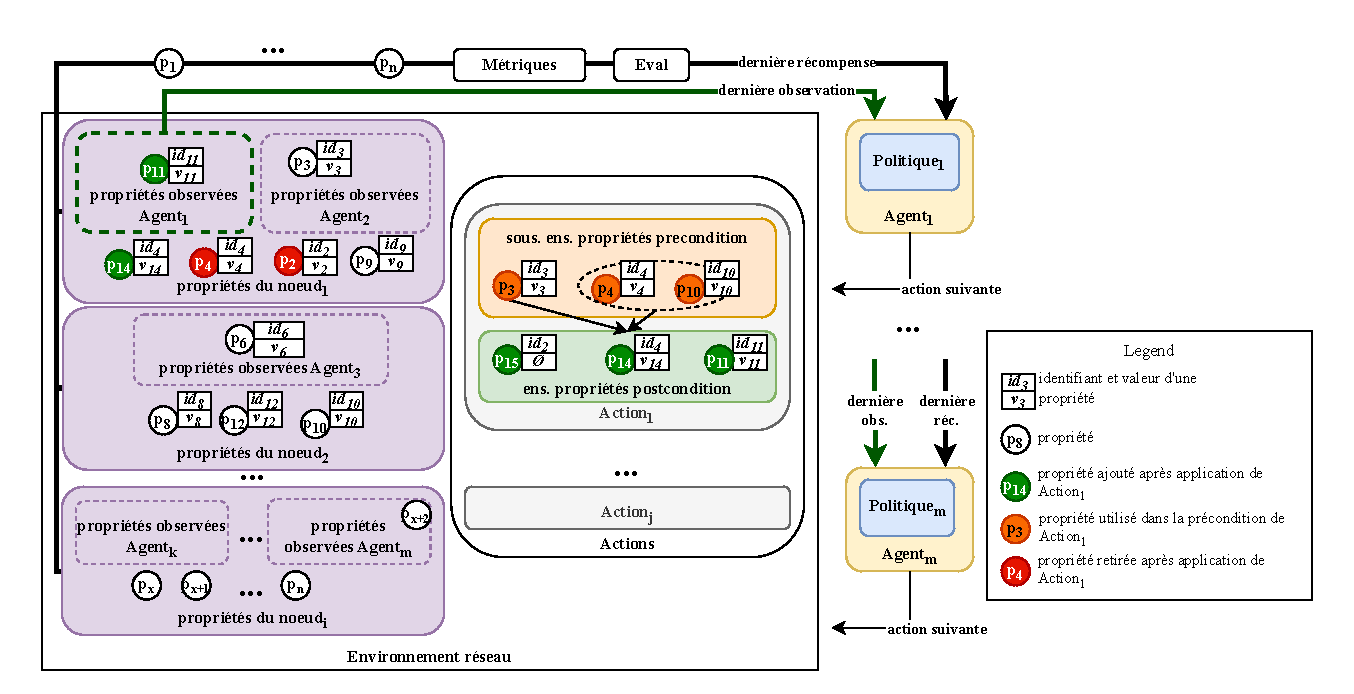
\includegraphics[trim=0.7cm 0.6cm 0.7cm 1cm, clip,width=1\textwidth]{figures/model_example_illustration.pdf}
    \caption{Vue illustrative du modèle de simulation}
    \label{fig:model_example_illustration}
\end{figure*}

\noindent
Le modèle \acn{Dec-POMDP} exprime l’état comme l’ensemble des propriétés des nœuds. Les actions sont définies par des pré/post-conditions sur ces propriétés. Les transitions et observations sont conditionnées par ces propriétés, et les récompenses sont calculées à partir de métriques sur l’état.

\subsubsection{Modélisation formelle Dec-POMDP}

Nous définissons les éléments liés aux propriétés des nœuds, des agents et des actions de l'environnement suivant :

\begin{itemize}

    \item $Ag = \{ag_1,..,ag_{|Ag|}\}$ : ensemble des agents (cyberattaquants et cyberdéfenseurs).
          % \begin{itemize}
          %     \item Avec $Attackers \subseteq Ag$ : l'ensemble des agents attaquants
          %     \item Avec $Defenders \subseteq Ag$ : l'ensemble des agents défenseurs
          % \end{itemize}

    \item Nous appelons le couple $p = (id_{j}, v_{j})$ avec $id_j \in {ID}$ et $v_j \in V$, une propriété.
          \begin{itemize}
              \item $\acn{ID}$ : l'ensemble des identifiants de propriétés indiquant éventuellement comment les propriétés sont organisées dans une structure de données non plate (telle que $PC1.processes.agents.agent1$). Ces identifiants de propriétés peuvent être utilisés pour un chemin d'accès à un fichier, le type de système d'exploitation utilisé dans un nœud, une ligne de commande utilisée par un agent\dots
              \item $V$ : Ensemble des valeurs de propriétés. Celles-ci peuvent inclure le contenu d'un fichier, une description complète du système d'exploitation, le résultat d'une ligne de commande\dots
                    % \item $Valeurs : \acn{ID} \rightarrow \mathcal{P}(V) = \{(id_{j}, V_{j}) \: | \: id_j \in {ID},$ $V_j \in \mathcal{P}(V)\}$ : une bijection associant un identifiant de propriété à l'ensemble des différentes valeurs auxquelles il peut être associé. Par exemple, l'identifiant $ls\_command\_output$ peut être associé aux valeurs suivantes $\{file.txt,\{file.txt,passwd.txt\}\}$
          \end{itemize}

    \item $P_{j} = \{ p_1, .., p_{|P_{j}|} \}$ : l'ensemble des propriétés $p_{l}$ (avec $l \in \{1,..,|P_{j}|\}$) du nœud $j$ ($j \in \mathbb{N} $). Par exemple, ces propriétés peuvent inclure certains identifiants de processus en cours d'exécution, la liste des fichiers d'un dossier, le type de système d'exploitation avec une description, des connaissances spécifiques d'un agent, etc.
          \begin{itemize}
              \item $P = P_1 \cup P_2 .. \cup P_{|P|} $ : Ensemble de toutes les propriétés des nœuds.
          \end{itemize}

    \item $Obs : \mathcal{P}(P) \times Ag \rightarrow \mathcal{P}(P_{Ag}), P_{Ag} \subset P$ : Relation qui associe les propriétés des nœuds et un agent au sous-ensemble de propriétés observées par l'agent.



    \item $Action : P_{pre} \rightarrow P_{post}$ : Relation qui associe un sous-ensemble de propriétés implicite dans une pré-condition booléenne conjonctive équivalente ($P_{pre} \subset \mathcal{P}(P)$) à un sous-ensemble de toutes les propriétés de la post-condition ($P_{post} \in \mathcal{P}(P)$). Par exemple, les propriétés $p_1 = (agent\_X\_privilege\_level, \allowbreak root)$, $p_2 = (agent\_X\_accessed\_text\_editor, \allowbreak Vim)$ et $p_3 = (agent\_X\_bashrc\_known\_filepath, \allowbreak /home/user/.bashrc)$ peuvent former une pré-condition ($p_1 \land p_2 \land p_3$) pour associer un nouvel ensemble de propriétés contenant $p4 = (bashrc\_file\_modified\_by\_X\_agent, \top)$. Deux sous-ensembles de pré-conditions peuvent être associés au même sous-ensemble de post-conditions pour modéliser une disjonction booléenne.

    \item $Metrics: \mathcal{P}(P) \times A \rightarrow \mathbb{R}^{n}$ : donne des métriques associées à un ensemble de propriétés et à une action conjointe. Par exemple, le nombre de nœuds encore actifs, les mouvements latéraux, etc.

\end{itemize}


En utilisant la description formelle d'un \acn{Dec-POMDP}~\cite{Oliehoek2016}, nous proposons le modèle \acn{Dec-POMDP} pré-spécialisé suivant :

\begin{itemize}
    \item $S = \{s_1, ..s_{|S|}\}, s_{i} \subseteq P \: et \: 1 \le i \le |S|$ : L'espace des états en tant qu'ensembles de propriétés possibles.

    \item $A_{i} = \{a_{i}^{1},..,a_{i}^{|A_{i}|}\}, a_{i}^j \in Action \: et \: 1 \le j \le |A_i|$ : l'ensemble des actions possibles pour l'agent $i$.

    \item $T$ : Ensemble des probabilités de transition conditionnelles entre les états
          \begin{itemize}
              \item Avec $T(s,a,s') = \probP(s'|s,a)$, la relation qui associe la probabilité d'aller de l'état $s \in S$ à l'état $s' \in S$ sachant que nous avons joué $a = (P^a_{pre} \times P^a_{post}) \in A$ avec $P^a_{pre} \subset \mathcal{P}(P)$ et $P^a_{post} \in \mathcal{P}(P)$
              \item Avec $\probP(s'|s,a) = 0$ si $s$ ne satisfait pas la condition préalable de $a$ (c'est-à-dire $\exists \: P_{pre_s}^{a} \in P_{pre}^{a} \: | \: P_{pre_s}^{a} \not\in \mathcal{P}(s)$).
              \item Avec $s' = (s - \{p_l=(id_l, v_l) \: | \: p_l \in s \: et$ $id_l \in \{id_k \: | \: (id_k, v_k) \in P^a_{post} \: et \: v_k \neq \varnothing\}\}) \cup P^a_{post}$
          \end{itemize}



    \item $R : S \times A \rightarrow \mathbb{R}^2 = Eval \circ Metrics$ : La fonction de récompense qui prend un état et une action et associe un indicateur de performance (à l'aide des métriques de l'état) pour les attaquants et les défenseurs.
          \begin{itemize}
              \item Avec $Eval : \mathbb{R}^{n} \rightarrow \mathbb{R}^2$, associe un vecteur métrique à une récompense pour les cyberattaquants et les cyberdéfenseurs.
          \end{itemize}



    \item $\Omega_{i} \subset Range(Obs \: | \: \{ (s, ag_i) | s \in S \: et \: ag_i \in Ag \}) \subset P$ : ensemble des propriétés observables pour l'agent $ag_i$. Par exemple, le contenu d'un fichier, la sortie du journal d'une commande, le résultat d'un scan de port, etc.
          \begin{itemize}
              \item $\Omega = \Omega_1 \cup \Omega_2 .. \cup \Omega_{|Ag|} = Range(Obs)$ : Ensemble de toutes les propriétés observables pour tous les agents.
          \end{itemize}

    \item $O$ : Ensemble des probabilités d'observation conditionnelles.
          \begin{itemize}
              \item Avec $O(s',a,o) = \probP(o|s',a)$, la relation qui associe la probabilité d'observer une observation $o \subset \Omega$ à partir de l'état $s' \in S$ induit par $a \in A$
              \item Avec $\probP(o|s',a) = 0$ si l'état $s' \in S$ ne contient pas les propriétés de $o \subset \Omega$ (c'est-à-dire $o \not\in \mathcal{P}(s')$). Par exemple, un agent joue l'action $x\_reads\_a\_log\_file$, ce qui donne lieu à un nouvel état dont une propriété appartenant à la connaissance de l'agent x est $(log\_file\_content\_known\_by\_x, \allowbreak abc)$. Cette propriété sera donc incluse dans les observations renvoyées à l'agent x.
          \end{itemize}

\end{itemize}


\subsubsection{Intégration des scénarios d’attaque/défense}

\noindent
D'un point de vue brut, la modélisation du Dec-POMDP pré-spécialisé proposée s'appuie sur des actions pour simuler la manière dont un système en réseau réel réagirait, y compris les vulnérabilités et les contre-mesures appliquées par les agents cyberattaquants et cyberdéfenseurs.

Un premier défi consiste à construire un scénario d'attaque/défense représentatif d'un système en réseau comportant des vulnérabilités afin de permettre de rendre une attaque en reliant les seules informations disponibles (telles que les tactiques, techniques et procédures connues de MITRE ATT\&CK) et en choisissant des contre-mesures de défense pertinentes (issues des mesures d'atténuation de MITRE ATT\&CK) et un environnement de déploiement. Un deuxième défi consiste à établir les actions correspondant au scénario d'attaque/défense. Comme les actions modifient les propriétés de l'environnement, elles ont également un impact sur l'espace des états possibles et les transitions entre ceux-ci.
De plus, lorsque l'on considère un faible niveau d'abstraction, de nombreuses actions simples peuvent permettre de décrire avec précision les changements opérés dans le réseau. Cependant, cela augmente le nombre d'actions, et encore plus le nombre d'états, car ceux-ci sont des combinaisons des effets des actions.

Ces défis sont directement liés aux questions étudiées concernant la génération automatisée de graphiques d'attaque à l'aide de bases de données disponibles intégrant éventuellement des techniques d'intelligence artificielle, comme dans ~\cite{GFalco2018}. Nous n'avons pas l'intention de nous attarder davantage sur ces questions, car elles dépassent le cadre de ce travail.

Ce modèle, illustrée en \autoref{fig:model_example_illustration}, permet de générer un simulateur multi-agents fidèle, où chaque action et observation est explicitement définie, facilitant l’extension à divers contextes de cyberdéfense.

\

\noindent
\textbf{Approche d'intégration MITRE ATT\&CK} : Nous suggérons une approche manuelle de haut niveau que nous avons utilisée pour intégrer les informations MITRE ATT\&CK sous forme d'arborescence AD, car elle formalise les actions à jouer dans un scénario et leurs interactions avec l'environnement. Elle vise à aider à établir les actions d'attaque/défense qui seront finalement intégrées dans le simulateur :
%
% \begin{enumerate*}[label=\arabic*),itemjoin={;\quad}]
\begin{itemize}
    \item Pour une menace persistante avancée (APT) donnée, nous avons identifié les tactiques, techniques et procédures pertinentes de MITRE ATT\&CK qui semblaient pertinentes pour un système en réseau

    \item Nous avons produit une description reliant les tactiques identifiées entre elles et les techniques, sous-techniques et procédures associées afin de créer un scénario décrivant comment le groupe APT pourrait attaquer le système en réseau. Cette étape définit la topologie du réseau avec ses principales propriétés
          (telles qu'un réseau d'entreprise composé de plusieurs serveurs de bases de données dédiés communiquant via FTP et HTTP, etc.)

    \item Nous avons créé une arborescence AD comme proposé dans ~\cite{BKordy2010} avec les tactiques comme objectifs d'action principaux et les techniques, sous-techniques et procédures dans la partie inférieure de l'arborescence. Nous avons veillé à disposer de plusieurs chemins pour atteindre un même objectif d'action principal. Nous avons pris soin de définir chaque action d'attaque avec des conditions préalables et des conditions postérieures basées sur les propriétés de l'environnement

    \item Nous avons extrait les techniques/sous-techniques MITRE ATT\&CK liées à la détection et aux mesures d'atténuation que nous avons ajoutées dans l'arbre AD afin d'enrichir les nœuds d'attaque. Nous avons veillé à définir chaque action de défense avec des conditions préalables et des conditions postérieures basées sur des propriétés dans l'environnement.

    \item Nous avons également répertorié et défini les principales actions environnementales spécifiques au déploiement à partir de la description précédente de l'environnement de déploiement ou des actions d'attaque/défense étendues qui sont communes aux cyberdéfenseurs et aux cyberattaquants. Cette étape permet d'obtenir un environnement plus réaliste, fournissant un nombre représentatif d'actions plausibles qu'un agent peut choisir dans de nombreux systèmes.
          Ces actions communes pourraient inclure au moins :
          \begin{enumerate*}[label=\arabic*),itemjoin={;\quad}]
              \item Lecture et écriture de fichiers
              \item Créer, supprimer, copier, déplacer, renommer, modifier les propriétés des fichiers/dossiers.
              \item Accéder à un dossier, accéder au dossier parent
              \item Sélectionner un fichier/dossier pour y appliquer des actions ultérieures
              \item Exécuter un fichier binaire
              \item Utilisation d'un protocole réseau (tel que HTTP, FTP, SSH, etc.).
              \item Autres interactions avec les lignes de commande de base concernant la surveillance ou le contrôle du système.
          \end{enumerate*}
          Ensuite, les propriétés environnementales associées doivent décrire un système de fichiers, une interface de terminal, un port avec des règles, les propriétés des paramètres du système d'exploitation, etc.
\end{itemize}

\section{Description et mise en oeuvre dans l'activité}
% Présenter l’algorithme générique de l’activité de modélisation (inputs → outputs).
% Inclure le pseudo-code / algorithme en environnement LaTeX comme dans l’ancien chapitre.

L’algorithme \ref{alg:modeling} décrit le déroulement général de l’activité de modélisation.
Chaque étape est explicitée ci-dessous afin d’en préciser les objectifs et le rôle dans la construction du modèle final.

\paragraph{Étape 1 : Formalisation manuelle des fonctions composantes.}
La première étape consiste à dériver manuellement, à partir des descriptions informelles de l’objectif global et des contraintes organisationnelles, trois fonctions fondamentales : la fonction de récompense $R^j_H$, la fonction d’arrêt $S^j_H$, et la fonction de rendu optionnelle $Render^j_H$.
Cette étape requiert l’expertise des concepteurs, qui doivent transformer des objectifs de haut niveau (souvent exprimés en langage naturel ou sous forme de règles métiers) en spécifications formelles permettant l’évaluation de trajectoires dans l’environnement simulé.

\paragraph{Étape 2 : Entraînement des auto-encodeurs pour les observations.}
Une fois les historiques d’interactions collectés, les observations conjointes $\Omega^j$ en sont extraites.
Comme leur dimension peut être très élevée dans un contexte multi-agent, elles sont compressées à l’aide d’auto-encodeurs.
L’encodeur $Enc_{\omega^j}$ apprend à transformer les observations en représentations latentes compactes $z_t$, tandis que le décodeur $Dec_{\omega^j}$ reconstruit les observations originales à partir de ces latents.
L’objectif est de minimiser l’erreur de reconstruction, garantissant ainsi que les latents conservent l’information essentielle.

\paragraph{Étape 3 : Encodage des observations dans les historiques.}
Les auto-encodeurs entraînés sont ensuite utilisés pour transformer l’ensemble des historiques $\mathcal{D}_{H^j}$ en séquences d’états latents.
Chaque observation $\omega_t^j$ est convertie en une représentation $z_t$, ce qui permet de constituer un nouvel ensemble d’entraînement $\mathcal{B}$ composé de triplets $(z_t, a_t^j, z_{t+1})$.
Cet encodage réduit la complexité des données d’entrée et prépare l’entraînement du modèle de dynamique.

\paragraph{Étape 4 : Entraînement du modèle de dynamique récurrent (RLDM).}
À partir de l’ensemble encodé $\mathcal{B}$, un modèle récurrent de dynamique latente (\acn{RLDM}) est entraîné.
Ce modèle, noté $\mathcal{T}^z$, apprend à prédire l’évolution des états latents en fonction de l’historique caché $\tilde{h}_{t-1}$, de l’état encodé courant $z_t$, et de l’action conjointe $a_t^j$.
L’entraînement se fait en minimisant l’erreur quadratique moyenne entre la prédiction $\hat{z}_{t+1}$ et le latent réel $z_{t+1}$.
Ce mécanisme d’apprentissage permet de capturer la dynamique de l’environnement sans accès direct à l’état global.

\paragraph{Étape 5 : Construction du JOPM.}
Une fois le \acn{RLDM} entraîné, les observations initiales $\Omega^{\mathcal{T}^j}_0$ sont extraites des historiques et utilisées pour initialiser le simulateur.
Le modèle de transition conjoint $\mathcal{T}^j$ est alors défini en combinant le modèle récurrent $f$, l’encodeur $Enc$, et le décodeur $Dec$.
Ainsi, pour toute observation et action donnée, $\mathcal{T}^j$ met à jour l’état caché et génère une observation prédite, constituant ainsi un simulateur complet des interactions multi-agents.

\paragraph{Étape 6 : Sorties de l’activité.}
Enfin, l’activité retourne l’ensemble des éléments modélisés : le modèle de transition conjoint $\mathcal{T}^j$, l’ensemble des observations initiales $\Omega^{\mathcal{T}^j}_0$, la fonction de récompense $R^j_H$, la fonction d’arrêt $S^j_H$, et la fonction de rendu éventuelle $Render^j_H$.
Ces composants constituent le cœur du jumeau numérique qui sera exploité par les activités d’entraînement, d’analyse et de transfert de la méthode \acn{MAMAD}.


\begin{algorithm}[H]
    \caption{Algorithme de l'activité de modélisation}
    \label{alg:modeling}
    \DontPrintSemicolon

    \KwIn{Historiques conjoints $\mathcal{D}_{H^j}$, objectif informel $\mathcal{G}_{\text{inf}}$, contraintes informelles $\mathcal{C}_{\text{inf}}$, facteur d'actualisation $\gamma$, espace des actions $A$, espace des observations $\Omega$}
    \KwOut{\acn{JOPM} $\mathcal{T}^j$, fonction de récompense $R^j_H$, spécifications MOISE+MARL $\mathcal{MM}$}

    \vspace{0.5em}
    \tcp{1. Formalisation manuelle des fonctions composantes}
    $(R^j_H, S^j_H, \text{Render}^j_H) \gets \texttt{manual\_formalize}(\mathcal{S}_{\text{inf}}, \mathcal{G}_{\text{inf}}, \mathcal{E}, A, \Omega)$ \;

    \vspace{0.5em}
    \tcp{2. Entraîner les auto-encodeurs pour les observations}
    Extraire les observations $\Omega^j = \{\omega^j_t\}$ à partir des historiques $\mathcal{D}_{H^j}$ \;
    Entraîner un auto-encodeur $(Enc_{\omega^j}, Dec_{\omega^j})$ sur $\Omega^j$ en minimisant l'erreur de reconstruction \;

    \vspace{0.5em}
    \tcp{3. Encoder les observations dans les historiques}
    Pour chaque historique $h^j = (\omega_t^j, a_t^j) \in \mathcal{D}_{H^j}$, encoder chaque observation conjointe ${z}_t = Enc_{\omega^j}(\omega^j_t)$ pour constituer l'ensemble d'entraînement $\mathcal{B} = \{ \{(z_t, a^j_t, z_{t+1})\} = h_z^j, h_z^j \in \mathcal{D}_{H^j}\}$

    \vspace{0.5em}
    \tcp{4. Entraîner le \acn{RLDM}}
    Initialiser le \acn{RLDM} $\mathcal{T}^z = f(g)$

    \For{$h_z^j \in \mathcal{B}$}{
        \For{$(z_t, a^j_t, z_{t+1}) \in h^j$}{
            Entraîner le \acn{RLDM} $\mathcal{T}^{z}$ en minimisant l'erreur quadratique moyenne (\acparen{MSE}) entre la prédiction $\hat{z}_{t+1}$ et la valeur réelle $z_{t+1}$.
        }
    }

    \vspace{0.5em}
    \tcp{5. Sauvegarder les observations initiales et former le JOPM}

    $\Omega^{\mathcal{T}^j}_0 \gets \{\omega^j_0\}$ extraites des historiques $\mathcal{D}_{H^j}$

    $\mathcal{T}^j(h_{t-1}, \omega_t, a_t) = \langle f(h_{t-1}, Enc(\omega^j_t), a^j_t), Dec(\mathcal{T}^{z}(h_{t-1}, Enc(\omega^j_t), a^j_t)) \rangle$ \;

    \vspace{0.5em}
    \tcp{6. Retourner les éléments modélisés}
    \Return{$\mathcal{T}^j, \Omega^{\mathcal{T}^j}_0, R^j_H, S^j_H, \text{Render}^j_H$}
\end{algorithm}



\section{Synthèse}

\noindent
En synthèse, l’activité de modélisation vise à fournir un environnement simulé fidèle et exploitable pour l’entraînement multi-agent, en combinant formalisme explicite (\acn{Dec-POMDP} générique) et génération automatique par World Models multi-agents. Les sorties produites — le modèle de transition conjoint (\acn{JOPM}), la fonction de récompense, la fonction d’arrêt et la fonction de rendu — constituent le socle du jumeau numérique utilisé dans les étapes suivantes. Cette approche permet d’assurer l’adaptation (via l’apprentissage sur données réelles), l’explicabilité (par la structure formelle du modèle) et la réutilisabilité (grâce au châssis générique). Toutefois, la fidélité du modèle dépend de la qualité et de la diversité des historiques collectés, et le coût computationnel de l’entraînement des auto-encodeurs et du \acn{RLDM} peut être élevé pour des environnements complexes. Enfin, la granularité des actions et la couverture des dynamiques réelles restent des limites inhérentes à toute simulation. L’activité d’entraînement exploitera ce modèle simulé pour optimiser les politiques sous contraintes organisationnelles, amorçant ainsi le cycle itératif de la méthode \acn{MAMAD}.

\clearpage
\thispagestyle{empty}
\null
\newpage

\chapter{Entraîner des politiques sous contraintes}
\label{chap:training}

L'\textit{activité d'entraînement} consiste à optimiser les politiques conjointes des agents dans l’environnement simulé, en tenant compte des contraintes organisationnelles.
Elle correspond à la phase de résolution du problème de conception, en exploitant les modèles produits par l’activité de modélisation.

Cette activité est cruciale car elle relie les critères définis dans \autoref{sec:criteres-evaluation} concernant la performance (C2), l’adaptation (C3),l’explicabilité (C5) et le contrôle (C4), via l’intégration de contraintes explicites dans l’apprentissage multi-agent.

\section*{Objectifs formels}

Les \textbf{entrées} de l’activité d’entraînement sont :
\begin{itemize}
    \item le modèle de transition conjoint $\mathcal{T}^j$ produit par la modélisation ;
    \item les observations initiales $\Omega^{\mathcal{T}^j}_0$ ;
    \item la fonction de récompense $R^j_H$ et la fonction d’arrêt $S^j_H$ ;
    \item les spécifications organisationnelles $\mathcal{MM}$ issues des contraintes informelles $\mathcal{C}_{\text{inf}}$ ;
    \item les espaces d’observations $\Omega$ et d’actions $A$ ;
    \item le facteur d’actualisation $\gamma$.
\end{itemize}

La \textbf{sortie attendue} est :
\begin{itemize}
    \item une politique conjointe entraînée $\pi^j = \{\pi^j_0, \pi^j_1, \dots, \pi^j_n\}$.
\end{itemize}

\noindent La relation globale peut s’exprimer par :
\begin{displaymath}
    \pi^j \gets \texttt{train}(\mathcal{T}^j, \Omega^{\mathcal{T}^j}_0, R^j_H, S^j_H, \text{Render}^j_H, \mathcal{MM}, \mathcal{C}_{\text{inf}}, \gamma, \Omega, A)
\end{displaymath}
\section{Travaux mobilisés et verrous identifiés}

L’activité d’entraînement des politiques sous contraintes s’appuie sur plusieurs familles de travaux issus du domaine du \acn{MARL} et de l’intégration de contraintes organisationnelles.

Du côté du \acn{MARL}, les méthodes classiques telles que l’apprentissage indépendant, l’apprentissage centralisé avec exécution décentralisée (\acn{CTDE}), ou encore les algorithmes de type Q-learning, Policy Gradient et leurs variantes multi-agents, constituent la base pour optimiser des politiques conjointes dans des environnements simulés. Ces approches sont efficaces pour maximiser la performance collective, mais elles n’intègrent pas nativement de contraintes organisationnelles explicites.

Pour pallier ce manque, plusieurs travaux issus du Safe \acn{RL} et des Constrained MDPs (\acn{CMDP}) ont été mobilisés. Les méthodes comme Constrained Policy Optimization (\acn{CPO}) ou Deep Constrained Q-Learning (\acn{DCQL}) permettent d’intégrer des contraintes numériques (sûreté, consommation, risque) dans le processus d’apprentissage, mais leur expressivité reste limitée à des contraintes locales et numériques, sans prise en compte de structures organisationnelles complexes.

Les approches de reward shaping, shielding, ou feedback humain offrent des mécanismes de guidage souple, permettant d’influencer indirectement les politiques apprises. Cependant, elles ne garantissent pas le respect formel de contraintes organisationnelles et restent difficiles à interpréter.

Enfin, les travaux sur l’intégration de modèles organisationnels symboliques, tels que $\mathcal{M}OISE^+$, proposent une formalisation riche des rôles, missions et relations collectives. Toutefois, leur intégration directe dans le processus d’apprentissage \acn{MARL} reste un verrou majeur, en raison de la difficulté à traduire ces spécifications en contraintes opérationnelles exploitables par les algorithmes d’apprentissage.

En synthèse, les principaux verrous identifiés sont :
\begin{itemize}
    \item l’absence de cadre unifié permettant d’intégrer des contraintes organisationnelles symboliques dans l’apprentissage \acn{MARL} ;
    \item la difficulté à garantir le respect de ces contraintes tout en maintenant la performance et l’adaptabilité des politiques ;
    \item le manque d’explicabilité et de contrôle sur les politiques apprises dans des environnements complexes et dynamiques.
\end{itemize}

\section{Positionnement et contributions proposées}

Pour lever ces verrous, notre approche propose d’hybrider les forces des cadres symboliques et connexionnistes en introduisant le framework MOISE+MARL. Ce cadre permet d’intégrer explicitement des spécifications organisationnelles (rôles, missions, permissions, obligations) dans le processus d’apprentissage multi-agent, en les traduisant sous forme de guides de contraintes (action masking, shaping de récompense, guides d’objectifs) injectés dans les algorithmes \acn{MARL}.

Notre contribution principale consiste à :
\begin{itemize}
    \item formaliser l’intégration des spécifications organisationnelles $\mathcal{M}OISE^+$ dans le \acn{MARL} via des guides de contraintes, permettant de restreindre ou d’orienter l’espace des politiques apprises ;
    \item proposer un nouveau formalisme, l’\acn{ODec-POMDP}, compatible avec les environnements simulés appris (World Models), pour permettre l’entraînement à partir de données observables uniquement ;
    \item développer un algorithme d’entraînement générique (voir Algorithme~\ref{alg:training_mamad}) qui articule ces guides de contraintes avec les méthodes \acn{MARL} existantes, assurant ainsi la compatibilité entre apprentissage connexionniste et respect des contraintes organisationnelles ;
    \item offrir un certain degré d’explicabilité et de contrôle sur les politiques apprises, grâce à la traçabilité des guides de contraintes et à l’analyse post-hoc des comportements émergents.
\end{itemize}

Ce positionnement permet de concilier performance, adaptation, contrôle et explicabilité dans l’entraînement des politiques multi-agents sous contraintes, ouvrant la voie à une conception plus robuste et transparente des \acn{SMA} pour des environnements critiques comme la cyberdéfense.

\subsection{MOISE+MARL pour lier $\mathcal{M}OISE^+$ avec le MARL}

\begin{figure}[h!]
    \centering
    \tikzset{every picture/.style={line width=0.75pt}} %set default line width to 0.75pt        

\begin{tikzpicture}[x=0.75pt,y=0.75pt,yscale=-1.2,xscale=1.4]
    %uncomment if require: \path (0,2584); %set diagram left start at 0, and has height of 2584

    %Straight Lines [id:da4973066741986565] 
    \draw [line width=1.5]    (118.21,2302.58) -- (203.1,2302) ;
    %Straight Lines [id:da14807114776731778] 
    \draw    (368.35,2272) -- (368.35,2294) -- (332.16,2294) ;
    \draw [shift={(330.16,2294)}, rotate = 360] [color={rgb, 255:red, 0; green, 0; blue, 0 }  ][line width=0.75]    (6.56,-1.97) .. controls (4.17,-0.84) and (1.99,-0.18) .. (0,0) .. controls (1.99,0.18) and (4.17,0.84) .. (6.56,1.97)   ;
    %Straight Lines [id:da16285043353898754] 
    \draw [line width=1.5]    (83.88,2398) -- (204.61,2398) ;
    %Straight Lines [id:da6299512000169913] 
    \draw    (169.94,2348) -- (204.61,2348) ;
    %Straight Lines [id:da64750232417664] 
    \draw    (84.65,2446) -- (383.15,2446) ;
    %Straight Lines [id:da35895220906699743] 
    \draw    (84.65,2230) -- (383,2230) ;
    %Straight Lines [id:da715014372569708] 
    \draw    (244.68,2262) -- (224.68,2262) -- (224.68,2408) ;
    \draw [shift={(224.68,2410)}, rotate = 270] [color={rgb, 255:red, 0; green, 0; blue, 0 }  ][line width=0.75]    (6.56,-1.97) .. controls (4.17,-0.84) and (1.99,-0.18) .. (0,0) .. controls (1.99,0.18) and (4.17,0.84) .. (6.56,1.97)   ;
    %Straight Lines [id:da71870438525014] 
    \draw    (251.96,2328) -- (286.51,2328) -- (286.51,2356) ;
    \draw [shift={(286.51,2358)}, rotate = 270] [color={rgb, 255:red, 0; green, 0; blue, 0 }  ][line width=0.75]    (6.56,-1.97) .. controls (4.17,-0.84) and (1.99,-0.18) .. (0,0) .. controls (1.99,0.18) and (4.17,0.84) .. (6.56,1.97)   ;
    %Straight Lines [id:da6006267784187092] 
    \draw [line width=0.75]  [dash pattern={on 0.84pt off 2.51pt}]  (252.87,2378) -- (252.87,2407) ;
    \draw [shift={(252.87,2410)}, rotate = 270] [fill={rgb, 255:red, 0; green, 0; blue, 0 }  ][line width=0.08]  [draw opacity=0] (5.36,-2.57) -- (0,0) -- (5.36,2.57) -- cycle    ;
    %Straight Lines [id:da8743336135156266] 
    \draw    (322.88,2304) -- (322.88,2316) ;
    \draw [shift={(322.88,2318)}, rotate = 270] [color={rgb, 255:red, 0; green, 0; blue, 0 }  ][line width=0.75]    (6.56,-1.97) .. controls (4.17,-0.84) and (1.99,-0.18) .. (0,0) .. controls (1.99,0.18) and (4.17,0.84) .. (6.56,1.97)   ;
    %Straight Lines [id:da14641229967966152] 
    \draw [line width=0.75]  [dash pattern={on 0.84pt off 2.51pt}]  (322.88,2378) -- (322.88,2407) ;
    \draw [shift={(322.88,2410)}, rotate = 270] [fill={rgb, 255:red, 0; green, 0; blue, 0 }  ][line width=0.08]  [draw opacity=0] (5.36,-2.57) -- (0,0) -- (5.36,2.57) -- cycle    ;
    %Straight Lines [id:da9260929933425808] 
    \draw [line width=0.75]  [dash pattern={on 0.84pt off 2.51pt}]  (286.51,2378) -- (286.51,2420) -- (312.61,2420) ;
    \draw [shift={(315.61,2420)}, rotate = 180] [fill={rgb, 255:red, 0; green, 0; blue, 0 }  ][line width=0.08]  [draw opacity=0] (5.36,-2.57) -- (0,0) -- (5.36,2.57) -- cycle    ;
    %Straight Lines [id:da3057006030233673] 
    \draw [line width=0.75]  [dash pattern={on 0.84pt off 2.51pt}]  (274,2449.7) -- (274,2457) ;
    \draw [shift={(274,2460)}, rotate = 270] [fill={rgb, 255:red, 0; green, 0; blue, 0 }  ][line width=0.08]  [draw opacity=0] (3.57,-1.72) -- (0,0) -- (3.57,1.72) -- cycle    ;
    %Straight Lines [id:da07288166228322246] 
    \draw    (342,2449.98) -- (342,2458) ;
    \draw [shift={(342,2460)}, rotate = 270] [color={rgb, 255:red, 0; green, 0; blue, 0 }  ][line width=0.75]    (6.56,-1.97) .. controls (4.17,-0.84) and (1.99,-0.18) .. (0,0) .. controls (1.99,0.18) and (4.17,0.84) .. (6.56,1.97)   ;
    %Shape: Ellipse [id:dp8508274348425935] 
    \draw   (95.09,2288.86) .. controls (95.09,2287.28) and (96.33,2286) .. (97.85,2286) .. controls (99.38,2286) and (100.62,2287.28) .. (100.62,2288.86) .. controls (100.62,2290.44) and (99.38,2291.71) .. (97.85,2291.71) .. controls (96.33,2291.71) and (95.09,2290.44) .. (95.09,2288.86) -- cycle ;
    %Straight Lines [id:da3825450168053828] 
    \draw    (97.85,2291.71) -- (97.85,2298.86) ;
    %Straight Lines [id:da521321206042058] 
    \draw    (97.85,2298.86) -- (93.71,2306) ;
    %Straight Lines [id:da055514206493922025] 
    \draw    (97.85,2298.86) -- (102,2306) ;
    %Straight Lines [id:da8996496708356774] 
    \draw    (102,2294.57) -- (93.71,2294.57) ;

    %Straight Lines [id:da31678488015771755] 
    \draw [line width=2.25]    (188,2454) -- (196.97,2454) ;
    \draw [shift={(201.97,2454)}, rotate = 180] [fill={rgb, 255:red, 0; green, 0; blue, 0 }  ][line width=0.08]  [draw opacity=0] (5.72,-2.75) -- (0,0) -- (5.72,2.75) -- cycle    ;
    %Shape: Ellipse [id:dp3927356466672782] 
    \draw   (238.88,2451.17) .. controls (238.88,2450.36) and (239.67,2449.7) .. (240.64,2449.7) .. controls (241.61,2449.7) and (242.4,2450.36) .. (242.4,2451.17) .. controls (242.4,2451.99) and (241.61,2452.65) .. (240.64,2452.65) .. controls (239.67,2452.65) and (238.88,2451.99) .. (238.88,2451.17) -- cycle ;
    %Straight Lines [id:da3365602555559104] 
    \draw    (240.64,2452.65) -- (240.64,2456.32) ;
    %Straight Lines [id:da7990875235744026] 
    \draw    (240.64,2456.32) -- (238,2460) ;
    %Straight Lines [id:da23945649338821617] 
    \draw    (240.64,2456.32) -- (243.28,2460) ;
    %Straight Lines [id:da11927353559661591] 
    \draw    (243.28,2454.12) -- (238,2454.12) ;

    %Straight Lines [id:da5816423191130675] 
    \draw    (251.96,2272) -- (252.85,2356) ;
    \draw [shift={(252.87,2358)}, rotate = 269.39] [color={rgb, 255:red, 0; green, 0; blue, 0 }  ][line width=0.75]    (6.56,-1.97) .. controls (4.17,-0.84) and (1.99,-0.18) .. (0,0) .. controls (1.99,0.18) and (4.17,0.84) .. (6.56,1.97)   ;
    %Straight Lines [id:da9310455126832857] 
    \draw    (321.97,2338) -- (321.97,2356) ;
    \draw [shift={(321.97,2358)}, rotate = 270] [color={rgb, 255:red, 0; green, 0; blue, 0 }  ][line width=0.75]    (6.56,-1.97) .. controls (4.17,-0.84) and (1.99,-0.18) .. (0,0) .. controls (1.99,0.18) and (4.17,0.84) .. (6.56,1.97)   ;
    %Shape: Rectangle [id:dp293492578719597] 
    \draw   (120,2453) .. controls (120,2451.34) and (121.34,2450) .. (123,2450) -- (127.72,2450) .. controls (129.37,2450) and (130.72,2451.34) .. (130.72,2453) -- (130.72,2457) .. controls (130.72,2458.66) and (129.37,2460) .. (127.72,2460) -- (123,2460) .. controls (121.34,2460) and (120,2458.66) .. (120,2457) -- cycle ;
    %Straight Lines [id:da33566712615128225] 
    \draw    (261.05,2262) -- (306,2262) ;
    \draw [shift={(308,2262)}, rotate = 180] [color={rgb, 255:red, 0; green, 0; blue, 0 }  ][line width=0.75]    (6.56,-1.97) .. controls (4.17,-0.84) and (1.99,-0.18) .. (0,0) .. controls (1.99,0.18) and (4.17,0.84) .. (6.56,1.97)   ;
    %Shape: Rectangle [id:dp28383270948937667] 
    \draw   (308,2236) -- (381.08,2236) -- (381.08,2276) -- (308,2276) -- cycle ;
    %Straight Lines [id:da18020989903965012] 
    \draw [line width=3]    (97.22,2282) -- (97.22,2270) ;
    \draw [shift={(97.22,2264)}, rotate = 90] [fill={rgb, 255:red, 0; green, 0; blue, 0 }  ][line width=0.08]  [draw opacity=0] (10.18,-4.89) -- (0,0) -- (10.18,4.89) -- cycle    ;
    %Straight Lines [id:da018421338049046554] 
    \draw [line width=3]    (97.22,2310) -- (97.11,2322.37) ;
    \draw [shift={(97.22,2328)}, rotate = 268.86] [fill={rgb, 255:red, 0; green, 0; blue, 0 }  ][line width=0.08]  [draw opacity=0] (10.18,-4.89) -- (0,0) -- (10.18,4.89) -- cycle    ;
    %Shape: Rectangle [id:dp7281037051878541] 
    \draw   (85.42,2450) -- (96.13,2450) -- (96.13,2460) -- (85.42,2460) -- cycle ;

    % Text Node
    \draw (362,2544.5) node  [font=\tiny] [align=left] {Role to constraint guide};
    % Text Node
    \draw (342,2524.5) node  [font=\tiny] [align=left] {Agents set};
    % Text Node
    \draw (342,2504.5) node  [font=\tiny] [align=left] {Actions set};
    % Text Node
    \draw (257,2584.5) node  [font=\tiny] [align=left] {Goal to constraint guide};
    % Text Node
    \draw (335,2484.5) node  [font=\tiny] [align=left] {Goals};
    % Text Node
    \draw (359,2564.5) node  [font=\tiny] [align=left] {Role to deontic specs.};
    % Text Node
    \draw (232,2564.5) node  [font=\tiny] [align=left] {Mission};
    % Text Node
    \draw (245,2544.5) node  [font=\tiny] [align=left] {Reward function};
    % Text Node
    \draw (248,2524.5) node  [font=\tiny] [align=left] {Goal-reward guide};
    % Text Node
    \draw (242,2504.5) node  [font=\tiny] [align=left] {Mission weight};
    % Text Node
    \draw (245,2484.5) node  [font=\tiny] [align=left] {Time constraints};
    % Text Node
    \draw (127,2584.5) node  [font=\tiny] [align=left] {Mission to goals};
    % Text Node
    \draw (129,2564.5) node  [font=\tiny] [align=left] {Role-reward guide};
    % Text Node
    \draw (128,2544.5) node  [font=\tiny] [align=left] {Role-action guide};
    % Text Node
    \draw (121,2524.5) node  [font=\tiny] [align=left] {Agent to role};
    % Text Node
    \draw (115,2504.5) node  [font=\tiny] [align=left] {Roles set};
    % Text Node
    \draw (122,2484.5) node  [font=\tiny] [align=left] {Deontic specs.};
    % Text Node
    \draw (310,2544) node  [font=\tiny] [align=left] {$\displaystyle \boldsymbol{rcg}$};
    % Text Node
    \draw (200,2504) node  [font=\tiny] [align=left] {$\displaystyle \mathcal{P}$};
    % Text Node
    \draw (200,2484) node  [font=\tiny] [align=left] {$\displaystyle \mathcal{T_{C}}$};
    % Text Node
    \draw (200,2564) node  [font=\tiny] [align=left] {$\displaystyle \mathcal{M}$};
    % Text Node
    \draw (77.5,2484) node  [font=\tiny] [align=left] {$\displaystyle \mathcal{DS}$};
    % Text Node
    \draw (310,2564) node  [font=\tiny] [align=left] {$\displaystyle \boldsymbol{rds}$};
    % Text Node
    \draw (310,2504) node  [font=\tiny] [align=left] {$\displaystyle \boldsymbol{A}$};
    % Text Node
    \draw (200,2544) node  [font=\tiny] [align=left] {$\displaystyle \boldsymbol{R}$};
    % Text Node
    \draw (310,2524) node  [font=\tiny] [align=left] {$\displaystyle \mathcal{A}$};
    % Text Node
    \draw (200,2524) node  [font=\tiny] [align=left] {$\displaystyle \boldsymbol{grg}$};
    % Text Node
    \draw (77.5,2564) node  [font=\tiny] [align=left] {$\displaystyle \boldsymbol{rrg}$};
    % Text Node
    \draw (77.5,2544) node  [font=\tiny] [align=left] {$\displaystyle \boldsymbol{rag}$};
    % Text Node
    \draw (200,2584) node  [font=\tiny] [align=left] {$\displaystyle \boldsymbol{gcg}$};
    % Text Node
    \draw (76.5,2524) node  [font=\tiny] [align=left] {$\displaystyle \boldsymbol{ar}$};
    % Text Node
    \draw (77,2584) node  [font=\tiny] [align=left] {$\displaystyle \boldsymbol{mo}$};
    % Text Node
    \draw (76.5,2504) node  [font=\tiny] [align=left] {$\displaystyle \mathcal{R}$};
    % Text Node
    \draw (310,2484) node  [font=\tiny] [align=left] {$\displaystyle \mathcal{G}$};


    % Text Node
    \draw  [fill={rgb, 255:red, 255; green, 255; blue, 255 }  ,fill opacity=1 ]  (241.82,2323) .. controls (241.82,2320.24) and (244.06,2318) .. (246.82,2318) -- (259.82,2318) .. controls (262.58,2318) and (264.82,2320.24) .. (264.82,2323) -- (264.82,2333) .. controls (264.82,2335.76) and (262.58,2338) .. (259.82,2338) -- (246.82,2338) .. controls (244.06,2338) and (241.82,2335.76) .. (241.82,2333) -- cycle  ;
    \draw (253.32,2328) node  [font=\scriptsize] [align=left] {$\displaystyle \boldsymbol{rcg}$};
    % Text Node
    \draw    (337,2252) -- (354,2252) -- (354,2272) -- (337,2272) -- cycle  ;
    \draw (345.5,2262) node  [font=\scriptsize] [align=left] {$\displaystyle \mathcal{Y}$};
    % Text Node
    \draw    (311,2252) -- (334,2252) -- (334,2272) -- (311,2272) -- cycle  ;
    \draw (322.5,2262) node  [font=\scriptsize] [align=left] {$\displaystyle \mathcal{T_{C}}$};
    % Text Node
    \draw    (357.39,2252) -- (378.39,2252) -- (378.39,2272) -- (357.39,2272) -- cycle  ;
    \draw (367.89,2262) node  [font=\scriptsize] [align=left] {$\displaystyle \mathcal{M}$};
    % Text Node
    \draw (347.43,2244) node  [font=\scriptsize] [align=left] {$\displaystyle \mathcal{DS}$};
    % Text Node
    \draw  [fill={rgb, 255:red, 255; green, 255; blue, 255 }  ,fill opacity=1 ]  (270,2257) .. controls (270,2254.24) and (272.24,2252) .. (275,2252) -- (288,2252) .. controls (290.76,2252) and (293,2254.24) .. (293,2257) -- (293,2267) .. controls (293,2269.76) and (290.76,2272) .. (288,2272) -- (275,2272) .. controls (272.24,2272) and (270,2269.76) .. (270,2267) -- cycle  ;
    \draw (281.5,2262) node  [font=\scriptsize] [align=left] {$\displaystyle \boldsymbol{rds}$};
    % Text Node
    \draw (158,2454.5) node  [font=\tiny] [align=left] {Relation name};
    % Text Node
    \draw (106.46,2454.5) node  [font=\tiny] [align=left] {Set};
    % Text Node
    \draw (255.47,2454.5) node  [font=\tiny] [align=left] {User};
    % Text Node
    \draw (216.32,2454.5) node  [font=\tiny] [align=left] {Define};
    % Text Node
    \draw (366.91,2454.5) node  [font=\tiny] [align=left] {Set relation};
    % Text Node
    \draw (306.61,2454.5) node  [font=\tiny] [align=left] {Impact on training};
    % Text Node
    \draw    (244.82,2410) -- (261.82,2410) -- (261.82,2430) -- (244.82,2430) -- cycle  ;
    \draw (253.32,2420) node  [font=\scriptsize] [align=left] {$\displaystyle \boldsymbol{A}$};
    % Text Node
    \draw    (314.84,2410) -- (331.84,2410) -- (331.84,2430) -- (314.84,2430) -- cycle  ;
    \draw (323.34,2420) node  [font=\scriptsize] [align=left] {$\displaystyle \boldsymbol{R}$};
    % Text Node
    \draw    (215.63,2410) -- (234.63,2410) -- (234.63,2430) -- (215.63,2430) -- cycle  ;
    \draw (225.13,2420) node  [font=\scriptsize] [align=left] {$\displaystyle \mathcal{A}$};
    % Text Node
    \draw  [fill={rgb, 255:red, 255; green, 255; blue, 255 }  ,fill opacity=1 ]  (309.97,2363) .. controls (309.97,2360.24) and (312.21,2358) .. (314.97,2358) -- (328.97,2358) .. controls (331.73,2358) and (333.97,2360.24) .. (333.97,2363) -- (333.97,2373) .. controls (333.97,2375.76) and (331.73,2378) .. (328.97,2378) -- (314.97,2378) .. controls (312.21,2378) and (309.97,2375.76) .. (309.97,2373) -- cycle  ;
    \draw (321.97,2368) node  [font=\scriptsize] [align=left] {$\displaystyle \boldsymbol{grg}$};
    % Text Node
    \draw    (274.56,2363) .. controls (274.56,2360.24) and (276.8,2358) .. (279.56,2358) -- (292.56,2358) .. controls (295.32,2358) and (297.56,2360.24) .. (297.56,2363) -- (297.56,2373) .. controls (297.56,2375.76) and (295.32,2378) .. (292.56,2378) -- (279.56,2378) .. controls (276.8,2378) and (274.56,2375.76) .. (274.56,2373) -- cycle  ;
    \draw (286.06,2368) node  [font=\scriptsize] [align=left] {$\displaystyle \boldsymbol{rrg}$};
    % Text Node
    \draw    (240.87,2363) .. controls (240.87,2360.24) and (243.11,2358) .. (245.87,2358) -- (259.87,2358) .. controls (262.63,2358) and (264.87,2360.24) .. (264.87,2363) -- (264.87,2373) .. controls (264.87,2375.76) and (262.63,2378) .. (259.87,2378) -- (245.87,2378) .. controls (243.11,2378) and (240.87,2375.76) .. (240.87,2373) -- cycle  ;
    \draw (252.87,2368) node  [font=\scriptsize] [align=left] {$\displaystyle \boldsymbol{rag}$};
    % Text Node
    \draw (156.15,2380.5) node  [font=\footnotesize] [align=left] {$\displaystyle  \begin{array}{{>{\displaystyle}l}}
                \ \ \boldsymbol{Constraint\ Guides} \\
                ( roles\ and\ goals\ logic)
            \end{array}$};
    % Text Node
    \draw  [fill={rgb, 255:red, 255; green, 255; blue, 255 }  ,fill opacity=1 ]  (309.93,2323) .. controls (309.93,2320.24) and (312.17,2318) .. (314.93,2318) -- (329.93,2318) .. controls (332.69,2318) and (334.93,2320.24) .. (334.93,2323) -- (334.93,2333) .. controls (334.93,2335.76) and (332.69,2338) .. (329.93,2338) -- (314.93,2338) .. controls (312.17,2338) and (309.93,2335.76) .. (309.93,2333) -- cycle  ;
    \draw (322.43,2328) node  [font=\scriptsize] [align=left] {$\displaystyle \boldsymbol{gcg}$};
    % Text Node
    \draw  [fill={rgb, 255:red, 255; green, 255; blue, 255 }  ,fill opacity=1 ]  (214.77,2323) .. controls (214.77,2320.24) and (217.01,2318) .. (219.77,2318) -- (227.77,2318) .. controls (230.53,2318) and (232.77,2320.24) .. (232.77,2323) -- (232.77,2333) .. controls (232.77,2335.76) and (230.53,2338) .. (227.77,2338) -- (219.77,2338) .. controls (217.01,2338) and (214.77,2335.76) .. (214.77,2333) -- cycle  ;
    \draw (223.77,2328) node  [font=\scriptsize] [align=left] {$\displaystyle \boldsymbol{ar}$};
    % Text Node
    \draw  [fill={rgb, 255:red, 255; green, 255; blue, 255 }  ,fill opacity=1 ]  (356.85,2289) .. controls (356.85,2286.24) and (359.08,2284) .. (361.85,2284) -- (374.85,2284) .. controls (377.61,2284) and (379.85,2286.24) .. (379.85,2289) -- (379.85,2299) .. controls (379.85,2301.76) and (377.61,2304) .. (374.85,2304) -- (361.85,2304) .. controls (359.08,2304) and (356.85,2301.76) .. (356.85,2299) -- cycle  ;
    \draw (368.35,2294) node  [font=\scriptsize] [align=left] {$\displaystyle \boldsymbol{mo}$};
    % Text Node
    \draw (127,2344.5) node  [font=\small] [align=left] {$\displaystyle  \begin{array}{{>{\displaystyle}l}}
                \mathbf{MOISE\ +MARL} \\
                \mathbf{Specs.\ Level}
            \end{array}$};
    % Text Node
    \draw (127,2422.5) node  [font=\small] [align=left] {$\displaystyle  \begin{array}{{>{\displaystyle}l}}
                \mathbf{MARL\ Level} \\
                \mathbf{(Dec-POMDP)}
            \end{array}$};
    % Text Node
    \draw    (243.91,2252) -- (260.91,2252) -- (260.91,2272) -- (243.91,2272) -- cycle  ;
    \draw (252.41,2262) node  [font=\scriptsize] [align=left] {$\displaystyle \mathcal{R}$};
    % Text Node
    \draw (182.64,2315) node  [font=\footnotesize] [align=left] {$\displaystyle \boldsymbol{Linkers}$};
    % Text Node
    \draw    (313.93,2284) -- (330.93,2284) -- (330.93,2304) -- (313.93,2304) -- cycle  ;
    \draw (322.43,2294) node  [font=\scriptsize] [align=left] {$\displaystyle \mathcal{G}$};
    % Text Node
    \draw (127,2261.5) node  [font=\small] [align=left] {$\displaystyle  \begin{array}{{>{\displaystyle}l}}
                \mathbf{{\displaystyle Org.\ Specs.\ Level}} \\
                {\displaystyle \ \ \ \ \ \ \ \ \ \ \ (\mathcal{M}\mathbf{OISE^+})}
            \end{array}$};


\end{tikzpicture}
    \caption[Vue minimale du framework MOISE+MARL]{Vue minimale du framework MOISE+MARL~: Les utilisateurs définissent d'abord les spécifications $\mathcal{M}OISE^+$, qui incluent les rôles ($\mathcal{R}$) et les missions ($\mathcal{M}$), tous deux associés via $rds$. Ils créent ensuite les spécifications MOISE+MARL en définissant d'abord des guides de contraintes tels que $rag$ et $rrg$ pour spécifier la logique des rôles, et $grg$ pour la logique des objectifs. Des linkers sont ensuite utilisés pour connecter les agents aux rôles via $ar$ et pour lier la logique des guides de contraintes aux spécifications $\mathcal{M}OISE^+$ définies. Une fois ces éléments configurés, les rôles peuvent être attribués aux agents, et le framework \acn{MARL} est mis à jour en conséquence pendant l'apprentissage.
    }
    \label{fig:mm_synthesis}
\end{figure}

\noindent MOISE+MARL introduit des moyens de contrôler ou de guider l'apprentissage des agents en \acn{MARL}. Sa principale contribution réside dans les \textbf{Guides de contraintes}, qui sont trois nouvelles relations introduites pour décrire la logique des rôles et des objectifs dans le formalisme \acn{Dec-POMDP} :
%
\begin{itemize}
    % \begin{enumerate*}[label={\roman*) },itemjoin={; \quad}]

    \item \textbf{Guide d'action des rôles} \quad $rag: H \times \Omega \rightarrow \mathcal{P}(A \times \mathbb{R})$, relation modélisant un rôle comme un ensemble de règles qui, pour chaque couple constitué d'un historique $h \in H$ et d'une observation reçue par l'agent $\omega \in \Omega$, associe des actions attendues $A \in \mathcal{P}(A)$ chacune associée à une contrainte de dureté $ch \in [0,1]$ ($ch = 1$ par défaut). En restreignant le choix de l'action suivante parmi celles autorisées, l'agent est contraint d'adhérer au comportement attendu du rôle
    \item \textbf{Guide de récompense des rôles} \quad $rrg: H \times \Omega \times A \to \mathbb{R} = \{r_m \text{ if } a \notin A_\omega \text{, } rag(h, \omega) \allowbreak = \allowbreak A_\omega \times \mathbb{R} \text{, } h \in H; \text{ else } 0\}$, la relation qui modélise un rôle en ajoutant une pénalité $r_m$ à la récompense globale si la dernière action choisie par l'agent $a \in A$ n'est pas autorisée. Ceci vise à encourager l'agent à adhérer au comportement attendu.
    \item \textbf{Guide de récompense d'objectif} \quad $grg: H \rightarrow \mathbb{R}$, la relation qui modélise un objectif comme une contrainte souple ajoutant un bonus de récompense $r_b \in \mathbb{R}$ si l'historique $h \in H$ de l'agent contient une sous-séquence caractéristique d'un objectif $h_g \in H_g$, encourageant l'agent à l'atteindre.
          % \end{enumerate*}
\end{itemize}

\noindent Enfin, nous introduisons les \textbf{Linkers} pour lier les spécifications organisationnelles $\mathcal{M}OISE^+$ aux guides de contraintes et aux agents :
%
\begin{itemize}
    % \begin{enumerate*}[label={\roman*) },itemjoin={; \quad}]

    \item \textbf{Agent vers Rôle} \quad $ar: \mathcal{A} \to \mathcal{R}$, la relation bijective reliant un agent à un rôle ;
    \item \textbf{Guide Rôle vers Contrainte} \quad $rcg: \mathcal{R} \rightarrow rag \cup rrg$, la relation associant chaque rôle $\mathcal{M}OISE^+$ à une relation $rag$ ou $rrg$, forçant/encourageant l'agent à suivre les actions attendues pour le rôle $\rho \in \mathcal{R}$ ;
    \item \textbf{Guide Objectif vers Contrainte} \quad $gcg: \mathcal{G} \rightarrow grg$, la relation reliant les objectifs aux relations $grg$, représentant les objectifs comme des récompenses dans \acn{MARL}.
          % \end{enumerate*}
\end{itemize}

\subsubsection*{Résolution du \acn{Dec-POMDP} avec MOISE+MARL}

Un modèle MOISE+MARL est défini par $\mathcal{MM} = \langle \mathcal{OS}, ar, rcg, gcg, rag, rrg, grg \rangle$.
La résolution d'un \acn{Dec-POMDP} avec $mm \in \mathcal{MM}$ consiste à trouver une politique conjointe $\pi^j = {\pi^j_0, \pi^j_1, \dots, \pi^j_n}$ qui maximise la récompense cumulative espérée (ou satisfait un seuil minimal), représentée par la fonction état-valeur $V^{\pi^j}$. Cette valeur reflète le rendement d'un état initial $s \in S$ lors de l'application d'actions conjointes successives $a^j \in A^n$ sous les contraintes organisationnelles supplémentaires.
%
La définition de $V^{\pi^j}$ suit le schéma d'exécution d'agent séquentiel et cyclique (mode \acn{AEC}) et est formalisée dans \hyperref[eq:single_value_function]{Définition 1}, intégrant des adaptations basées sur les rôles (en rouge) et les missions (en bleu) qui influencent à la fois l'espace d'action et la récompense.
\autoref{fig:mm_synthesis} illustre comment les spécifications $\mathcal{M}OISE^+$ sont intégrées à la résolution \acn{Dec-POMDP} via le cadre MOISE+MARL.


\begin{figure*}[h!]
    \label{eq:single_value_function}
    \raggedright
    \textbf{\textit{Definition 1} \quad Fonction État-Valeur adaptée aux guides de contraintes en \acn{AEC} :}

    \begin{scriptsize}
        \vspace{-0.6cm}
        \begin{gather*}
            V^{\pi^j}(s_t) = \hspace{-0.75cm}
            %
            \sum_{\textcolor{red}{ \substack{a_{t} \in A \text{ if } rn() < ch_{t}, \\
                        a_{t} \in A_{t} \text{ else}}
                }}{\hspace{-0.7cm} \pi_i(a_{t} | \omega_t)}
            %
            \sum_{s_{t+1} \in S}
            %
            {\hspace{-0.1cm} T(s_{t+1} | s_t, a_{t})
            \Bigl[R(s_t,a_{t},s_{t+1}) + \hspace{-0.1cm}
            \textcolor{blue}{ \sum_{m \in \mathcal{M}_i}{ \hspace{-0.1cm} v_m(t) \frac{grg_m(h_{t+1})}{1 - p + \epsilon} } }
            + } \\
            {\textcolor{red}{(1-ch_t) \times rrg(\omega_t,a_{t+1})} + V^{\pi^j_{i+1 \ mod \ n}}(s_{t+1})\Bigr]}
        \end{gather*}
        %
        \vspace{-0.5cm}
        \textcolor{red}{\[\text{ \hspace{-0.1cm} Avec } rag(h_t, \omega_t) = A_{t} \times \mathbb{R} \text{, } \langle a_t, ch_{t} \rangle \in A_{t} \times \mathbb{R} \text{ ; } rn: \emptyset \to [0,1[ \text{, une fonction aléatoire uniforme}\]}
        %
        \vspace{-0.6cm}
        \textcolor{blue}{
            \begin{gather*}
                \hspace{-0.001cm}
                \text{Avec } \omega_t = O(\omega_t | s_t, a_t) \text{ ; } h_t = \{h_0 = \langle \rangle, h_{t+1} = \langle h_t, \langle \omega_{t+1}, a_{t+1} \rangle \rangle \} \text{ ; } \epsilon \in \mathbb{R}_{>0} \text{ ; } grg_m(h) =
            \end{gather*}
        }
        \vspace{-0.95cm}
        \textcolor{blue}{
            \begin{gather*}
                \hspace{-0.5cm} \sum_{\hspace{0.3cm}(grg_i,w_i) \in mo(m)}{\hspace{-0.9cm} w_i \times grg_i(h)}
                \text{ ; } v_m(t) = \{ 1 \text{ if } t \in t_c \text{ ; else } 0 \} \text{ ; } \mathcal{M}_i = \{m_j | \langle ar(i),m_j,t_c,p \rangle \in \mathcal{M}\}
            \end{gather*}
        }
        \vspace{-0.6cm}
    \end{scriptsize}

\end{figure*}

À chaque pas de temps $t \in \mathbb{N}$ (à partir de $t=0$), l'agent $i = t \bmod n$ se voit attribuer le rôle $\rho_i = ar(i)$. Pour chaque spécification déontique temporellement valide $d_i = rds(\rho_i) = \langle tc_i, y_i, m_i \rangle$, l'agent est autorisé ($y_i = 0$) ou obligé ($y_i = 1$) à s'engager dans la mission $m_i \in \mathcal{M}$, avec un objectif $\mathcal{G}_{m_i} = mo(m_i)$ et $n \in \mathbb{N}$ agents.
%
En observant $\omega_t$, l'agent sélectionne une action parmi $A_t$ (actions attendues par le rôle) avec une probabilité $ch_t$, ou parmi $A$ sinon. Si $ch_t = 1$, l'agent est strictement contraint par son rôle.
%
L'action sélectionnée fait passer le système de $s_t$ à $s_{t+1}$, génère l'observation $\omega_{t+1}$ et renvoie une récompense composée de :
i) des bonus pour les objectifs atteints dans les missions valides (via les guides de récompenses d'objectifs), pondérés par $\frac{1}{1 - p + \epsilon}$ ;
ii) des pénalités du guide de récompenses de rôle, échelonnées par $ch_t$.
%
Le processus se poursuit dans l'état $s_{t+1}$ avec l'agent $(i + 1) \bmod n$.

\subsubsection*{Faciliter l'implémentation des \textbf{Guides de contraintes}}

Puisque les rôles, objectifs et missions sont de simples étiquettes, leur définition est implicite. Cependant, implémenter une relation \(rag\), \(rrg\) ou \(grg\) nécessite de définir de nombreux historiques, souvent redondants, rendant une définition extensionnelle fastidieuse. De plus, la logique de chaque \textbf{Guide de contraintes} analyse la trajectoire de l'agent pour vérifier son appartenance à un ensemble prédéfini. Par exemple, \(rag\) détermine les actions attendues selon l'appartenance de la trajectoire à un ensemble donné et la nouvelle observation.

Une approche consiste à laisser l'utilisateur définir ses \textbf{Guides de contraintes} via une logique personnalisée (par script, par exemple). Dans ce cas, la relation \(b_g: H \to \{0,1\}\) formalise la décision d'appartenance d'un historique à un ensemble \(H_g\).
Pour simplifier l'implémentation, nous proposons un \acn{TP}, inspiré du Traitement Automatique du Langage, noté \(p \in P\), permettant de définir intentionnellement un ensemble d'historiques.

Un \acn{TP} implique que toute observation ou action réelle considérée est connue et associée à une étiquette \(l \in L\) (via \(l: \Omega \cup A \to L\)) afin d'être gérée de manière pratique. Un \acn{TP} \(p \in P\) est défini comme suit : \(p\) est soit une « séquence feuille » notée comme un couple historique-cardinalité \(s_l = \langle h, \{c_{min}, c_{max}\} \rangle\) (où \(h \in H\), \(c_{min} \in \mathbb{N}\), \(c_{max} \in \mathbb{N} \cup \{``*"\}\)) ; soit une « séquence nœud » notée comme un couple composé d'un tuple de séquences et d'une cardinalité \(s_n = \langle \langle s_{l_1}, s_{l_2}, \dots \rangle, \{c_{min}, c_{max}\} \rangle\). Par exemple, le pattern
$
    p = ``[o_1,a_1,[o_2,a_2]\langle0,2\rangle]\langle1,*\rangle"
$
peut être formalisé comme la séquence nœud
$
    \langle \langle \langle o_1,a_1\rangle,\langle 1,1 \rangle \rangle, \langle \langle o_2,a_2\rangle,\langle 0,2 \rangle \rangle \rangle \langle 1,``*"\rangle,
$
indiquant l'ensemble des historiques \(H_p\) contenant au moins une fois la sous-séquence constituée d'une première paire \(\langle o_1,a_1\rangle\) suivie d'au maximum deux répétitions de la paire \(\langle o_2,a_2\rangle\).

\subsection{Extension de MOISE+MARL aux \textit{World Models} Multi-Agents}

\noindent Dans des environnements réalistes, on ne dispose que des transitions issues des historiques d'actions et d'observations reçues. Pour mieux représenter ce contexte, nous introduisons un nouveau formalisme appelé \textbf{\acn{Dec-POMDP} basé sur les observations} (\acparen{ODec-POMDP}). Un \acn{ODec-POMDP} $d_\Omega \in OD_\Omega$ (avec $OD_\Omega$, l'ensemble des ODec-POMDPs) est défini comme un quintuplet~:
%
$d_\Omega = \left(\Omega, A, \mathcal{T}^j, R^j_H, \gamma \right)$
%
où~:
\begin{itemize}
    \item $A$~: l'espace d'actions.
    \item $\Omega$~: l'espace d'observations.
    \item $\Omega^{\mathcal{T}^j}_0$~: l'ensemble des observations initiales conjointes.
    \item $\mathcal{T}^j(h, \omega, a) = \langle \tilde{h}', \mathbb{P}(\omega' \mid h, \omega, a) \rangle$~: le \acn{JOPM} estimant la prochaine observation conjointe $\omega'$ à partir de l'historique $\tilde{h} \in \mathcal{H}$, de l'observation conjointe actuelle $\omega$ et de l'action conjointe $a$. Le modèle renvoie également l'état caché récurrent mis à jour $\tilde{h}'$.
    \item $R^j_H~: H \times \Omega \times A \times \Omega \rightarrow \mathbb{R}$~: la fonction de récompense basée sur l'historique, calculant la récompense depuis l'historique précédent, l'observation et action courante et l'observation suivante.
    \item $\gamma \in [0, 1]$~: le facteur d'actualisation.
\end{itemize}

\noindent Cette formulation permet aux agents \acn{MARL} d'opérer uniquement à partir de données observables, rendant la méthode compatible avec les environnements simulés appris.

\subsubsection*{Résolution d'un \acn{ODec-POMDP} avec MOISE+MARL}

Résoudre un \acn{ODec-POMDP} avec des contraintes $mm \in \mathcal{MM}$ consiste à trouver une politique conjointe $\pi^j = \{\pi^j_0, \pi^j_1, \dots, \pi^j_n\}$ qui maximise la récompense cumulée espérée (ou qui satisfait un seuil minimal), via la fonction de valeur basée sur les observations $V_{\mathcal{T}^j}^{\pi^j}$. Cette fonction représente le retour attendu depuis une observation conjointe initiale $\omega^j \in \Omega^{\mathcal{T}^j}_0$, un historique $h^j$ et un état caché $\tilde{h}$, en appliquant des actions conjointes $a^j \in A^n$ sous contraintes organisationnelles $\mathcal{MM}$, et en utilisant $\mathcal{T}^j$ pour approximer les transitions.

La définition complète de $V_{\mathcal{T}^j}^{\pi^j}$ est donnée dans \hyperref[eq:single_value_function_parallel]{Définition 2}, et intègre les adaptations basées sur les rôles (en rouge) et sur les missions (en bleu), qui influencent à la fois l'espace d'actions conjointes et la récompense. La \autoref{fig:mm_synthesis} illustre comment les spécifications $\mathcal{M}OISE^+$ sont injectées dans la résolution d'un \acn{ODec-POMDP} à l'aide du cadre MOISE+MARL.

\medskip

\begin{figure*}[h!]
    \label{eq:single_value_function_parallel}
    \raggedright
    \textbf{\textit{Definition 2} \quad Fonction Observation-Valeur adaptée aux guides de contraintes en mode parallèle:}

    \begin{scriptsize}
        \vspace{-0.6cm}
        \begin{gather*}
            \hspace{-1cm}V^{\pi^j}(\tilde{h}_{t-1},h^j_{t-1},\hat{\omega}^j_t) = \hspace{-0.95cm}
            %
            \sum_{\textcolor{red}{ \substack{a^j_{t} \in A^j \text{ if } rn() < ch_{t}, \\
            a^j_{t} \in A^j_{t} \text{ else}}
            }}{\hspace{-0.9cm} \pi_i(a^j_{t} | \hat{\omega}^j_t)}
            %
            \hspace{-1.2cm}
            \sum_{\phantom{XXXX}(\tilde{h}_t,\hat{\omega}^j_{t+1}) \in \mathcal{H} \times \hat{\Omega}^j}
            %
            {\hspace{-1.2cm} \mathcal{T}^j(\langle \tilde{h}_t,\hat{\omega}^j_{t+1} \rangle | \tilde{h}_{t-1}, \hat{\omega}_t, a^j_{t})
            \Bigl[R^j_H(h^j_{t-1},\hat{\omega}^j_t,a^j_t,\hat{\omega}^j_{t+1}) \hspace{-0.1cm} }
        \end{gather*}
        %
        \vspace{-1cm}
        \begin{gather*}
            \hspace{3cm}
            {+ \  \textcolor{blue}{grg^j_m(h^j_t)}
            +
            \textcolor{red}{(1-ch_t) \times rrg^j(\hat{\omega}^j_t,a^j_{t+1})} + V^{\pi^j}(\tilde{h}_{t}, h^j_t, \hat{\omega}^j_{t+1})\Bigr]}
        \end{gather*}
        %
        \vspace{-0.15cm}
        %
        \[\hspace{-0.9cm}\text{Avec \ } \tilde{h}_{-1} = \mathbf{0} \text{ and } \tilde{\omega}^j_0 \in \Omega_0^{\mathcal{T}^j} \text{ ; } a^j_t = \langle a_{t,0}, a_{t,1} \dots a_{t,|\mathcal{A}|} \rangle \text{ ; } \omega^j_t = \langle \omega_{t,0}, \omega_{t,1} \dots \omega_{t,|\mathcal{A}|} \rangle \text{ ; }\]
        %
        \vspace{-0.25cm}
        \[\hspace{-0.5cm} h^j_t = \langle h_{t,0}, h_{t,1} \dots h_{t,|\mathcal{A}|} \rangle = \langle \langle h_{t-1,i}, \omega_{t,i}, a_{t,i} \rangle \rangle_{i \in \mathcal{A}}\]
        %
        \vspace{-0.2cm}
        \textcolor{red}{\[\hspace{-1cm}\text{ \hspace{-0.1cm} Avec } \langle rag_i, rrg_i \rangle = rcg(ar(i)) \text{ ; } rn: \emptyset \to [0,1[ \text{, une fonction aléatoire uniformef}\]}
        %
        \vspace{-0.3cm}
        \textcolor{red}{\[A^j_t \times \mathbf{R}^{|\mathcal{A}|} = rag^j(h^j_t, \tilde{\omega}^j_t) = \langle rag_i(h_{t,i}, \omega_{t,i}) \rangle_{i \in \mathcal{A}} \text{ ; } rrg^j(h^j_t, \tilde{\omega}^j_t, a^j_t) = \sum_{i \in \mathcal{A}}{rrg_i(h_{t,i}, \omega_{t,i}, a_{t,i})}\]}
        %
        \vspace{-0.75cm}
        \textcolor{blue}{
            \begin{gather*}
                \hspace{-1cm} grg_m(h) = \hspace{-1cm} \sum_{\hspace{0.3cm}(grg_i,w_i) \in mo(m)}{\hspace{-1.1cm} w_i \times grg_i(h)}
                \text{ ; }
                grg^j_m(h^j_t) = \hspace{-0.1cm} \sum_{i \in \mathcal{A}}{\sum_{m \in \mathcal{M}_i}{ \hspace{-0.1cm} v_m(t) \frac{grg_m(h_{t,i})}{1 - p + \epsilon} }} \text{ ; } \epsilon \in \mathbb{R}_{>0} \text{ ; }
            \end{gather*}
        }
        \vspace{-0.9cm}
        \textcolor{blue}{
            \begin{gather*}
                \hspace{-1cm}
                v_m(t) = \{ 1 \text{ if } t \in t_c \text{ ; else } 0 \} \text{ ; } \mathcal{M}_i = \{m_j | \langle ar(i),m_j,t_c,p \rangle \in \mathcal{M}\}
            \end{gather*}
        }
    \end{scriptsize}

\end{figure*}

\noindent En mode parallèle, à chaque pas de temps $t \in \mathbb{N}$ (en commençant à $t=0$), chaque agent $i \in \mathcal{A}$ est assigné à un rôle $\rho_i = ar(i)$. Pour chaque spécification déontique temporellement valide $d_i = rds(\rho_i) = \langle tc_i, y_i, m_i \rangle$, l'agent est soit autorisé ($y_i = 0$), soit obligé ($y_i = 1$) de s'engager dans la mission $m_i \in \mathcal{M}$, avec ensemble d'objectifs $\mathcal{G}_{m_i} = mo(m_i)$.

Lorsque les agents observent $\tilde{\omega}_t^j$, ils sélectionnent leurs actions dans $A_{i,t}$ (dérivées via les guides de récompense de rôle) avec une probabilité $ch_t$, ou dans $A_t$ sinon. Si $ch_t = 1$, les agents sont strictement contraints par leur rôle.

Les transitions d'observation et d'état sont approximées via la fonction $\mathcal{T}^j$ à partir de l'état caché précédent $\tilde{h}_{t-1}$, de l'observation conjointe $\omega^j_t$ et de l'action conjointe $a^j_t$. La fonction de récompense $R^j_H$ utilise ces mêmes informations, ainsi que l'observation suivante, pour produire la récompense. Des bonus ou malus sont ensuite ajoutés selon~:
i) l'atteinte d'objectifs valides (via les guides de récompense des objectifs, pondérés par $\frac{1}{1 - p + \epsilon}$),
ii) la conformité au rôle (via les guides de récompense de rôle, pondérés par $1 - ch_t$).


\section{Description et mise en oeuvre dans l'activité}

L’algorithme~\ref{alg:training_mamad} décrit le déroulement général de l’activité d’entraînement.
Chaque étape est détaillée ci-après.

\paragraph{Étape 1 : Formalisation des contraintes.}
Si les spécifications $\mathcal{MM}$ ne sont pas fournies, elles sont dérivées manuellement à partir des contraintes informelles $\mathcal{C}_{\text{inf}}$.

\paragraph{Étape 2 : Initialisation.}
Initialiser les paramètres de la politique conjointe $\pi^j$ et un buffer d’expérience $\mathcal{B}$.

\paragraph{Étape 3 : Exécution d’épisodes simulés.}
Pour chaque épisode, échantillonner une observation initiale $\omega_0^j \in \Omega^{\mathcal{T}^j}_0$, initialiser l’historique $h_{-1}^j$ et l’état caché $\tilde{h}_{-1}$.

\paragraph{Étape 4 : Sélection des actions sous contraintes.}
À chaque étape $t$, calculer l’ensemble des actions autorisées $A_t^j = rag^j(h^j_t,\omega_t^j)$.
L’agent sélectionne son action $a_t^j$ parmi $A_t^j$ avec probabilité $ch_t$, sinon dans $A$.

\paragraph{Étape 5 : Transition et mise à jour du JOPM.}
La transition $(\tilde{h}_t,\omega_{t+1}^j)$ est générée par $\mathcal{T}^j(\tilde{h}_{t-1},\omega_t^j,a_t^j)$.

\paragraph{Étape 6 : Calcul des récompenses.}
La récompense $r_t$ combine :
\begin{itemize}
    \item la récompense de base $R^j_H$,
    \item un bonus $grg^j(h^j_t)$ si des objectifs sont atteints,
    \item un bonus/malus $(1-ch_t)\times rrg^j(h^j_t,\omega_t^j,a_t^j)$ lié au respect du rôle.
\end{itemize}

\paragraph{Étape 7 : Mise à jour de l’expérience et apprentissage.}
Les transitions sont stockées dans $\mathcal{B}$, et la politique $\pi^j$ est optimisée par tout algorithme \acn{MARL} compatible (Q-learning, Policy Gradient, \acn{CTDE}, etc.).

\paragraph{Étape 8 : Sortie.}
À la fin des épisodes, l’activité retourne la politique conjointe entraînée $\pi^j$.


\begin{algorithm}[H]
    \caption{Algorithme de l'activité d'entraînement}
    \label{alg:training_mamad}
    \DontPrintSemicolon

    \KwIn{
    Modèle de Prédiction d'Observations Conjointes (\acn{JOPM}) $\mathcal{T}^j$,
    Observations initiales conjointes $\Omega_0^{\mathcal{T}^j}$,
    Fonction de récompense $R_H^j$,
    Fonction d'arrêt $S_H^j$,
    Fonction de rendue $\text{Render}^j_H$,
    Spécifications organisationnelles $\mathcal{MM}$,
    Contraintes de conception informelles $\mathcal{C}_{\text{inf}}$,
    Facteur d'actualisation $\gamma$
    Espace d'observations $\Omega$,
    Espace d'actions $A$
    }
    \KwOut{$\pi^j$~: Politique conjointe entraînée}

    \vspace{0.3em}

    \If{$\mathcal{MM} = \emptyset$}{
        $\mathcal{MM} \gets \texttt{manual\_formalize}(\mathcal{C}_{\text{inf}})$ \tcp*{Formalisation manuelle specs. orgs.} \;
    }

    Initialiser les paramètres de la politique $\pi^j$ et du buffer de replay $\mathcal{B}$ \;

    \ForEach{épisode $e = 1 \dots N$}{
    Échantillonner $\omega_0^j \sim \Omega_0^{\mathcal{T}^j}$, initialiser $\tilde{h}_{-1} \gets \mathbf{0}$ \;
    Initialiser l'historique $h_{-1}^j \gets \emptyset$ \;

    \ForEach{étape $t = 0 \dots T$}{
    Calculer $A_t^j = rag^j(h^j_t, \omega^j_t)$ via les guides de récompense de rôle dans $\mathcal{MM}$ \;
    \If{$rn() < ch_t$}{
        Sélectionner $a_t^j \sim \pi^j(\cdot | \omega_t^j)$ dans l'ensemble $A_t^j$ (contraint) \;
    }
    \Else{
        Sélectionner $a_t^j \sim \pi^j(\cdot | \omega_t^j)$ dans l'ensemble $A_t$ \;
    }

    $(\tilde{h}_t, \omega_{t+1}^j) \gets \mathcal{T}^j(\tilde{h}_{t-1}, \omega_t^j, a_t^j)$ \tcp*{Prédiction JOPM}

    $r_t \gets \gamma^t \times R_H^j(h^j_{t-1}, \omega_t^j, a_t^j, \omega_{t+1}^j)$ \tcp*{Récompense de base}

    $r_t \gets r_t + grg^j(h^j_t)$ \tcp*{Bonus via guides d'objectifs}

    $r_t \gets r_t + (1 - ch_t) \times rrg^j(h^j_t, \omega_t^j, a_t^j)$ \tcp*{Bonus/malus via guides de rôle}

    Ajouter $(\omega_t^j, a_t^j, r_t, \omega_{t+1}^j)$ à $\mathcal{B}$ \;
    Mettre à jour $h^j_t \gets \langle \langle h_{t-1,i}, \omega_{t,i}, a_{t,i} \rangle \rangle_{i \in \mathcal{A}}$ \;

    Entraîner $\pi^j$ avec des mini-lots tirés de $\mathcal{B}$ en utilisant toute méthode \acn{MARL} \;
    }
    }

    \Return{$\pi^j$}
\end{algorithm}



\section{Synthèse}

En synthèse, l’activité d’entraînement permet de produire des politiques conjointes optimisées, intégrant à la fois les contraintes organisationnelles explicites et les dynamiques apprises via les World Models multi-agents.
Cette approche concilie performance et adaptation tout en offrant un certain degré de contrôle et d’explicabilité.

Les principales limites identifiées concernent :
\begin{itemize}
    \item la scalabilité du \acn{MARL} contraint à un grand nombre d’agents ;
    \item la dépendance aux données disponibles pour apprendre un \acn{JOPM} fidèle ;
    \item le compromis entre respect strict des contraintes et performance optimale.
\end{itemize}

Ces éléments préparent l’\textbf{activité d’analyse}, qui vise à évaluer et expliciter les politiques entraînées.


\clearpage
\thispagestyle{empty}
\null
\newpage

\chapter{Analyser les comportements émergents}
\label{chap:analyzing}

L'\textit{activité d’analyse} vise à évaluer et expliciter les politiques conjointes apprises. Elle fournit une explication des comportements observés en termes de rôles, objectifs et missions. Cette activité joue un rôle central pour l’explicabilité en reliant les dynamiques apprises aux structures organisationnelles interprétables.


\section*{Objectifs formels}


Les \textbf{entrées} de l’activité d’analyse sont :
\begin{itemize}
    \item une politique conjointe entraînée $\pi^j$ ;
    \item un \acn{ODec-POMDP} $d_\Omega$ représentant l’environnement simulé appris ;
    \item une spécification organisationnelle initiale $\mathcal{MM}$ (optionnelle).
\end{itemize}

Les \textbf{sorties attendues} sont :
\begin{itemize}
    \item une spécification implicite inférée $\mathcal{MM}_{\text{implicit}}$ ;
    \item un score d’adéquation organisationnelle $\text{OF}$.
\end{itemize}

\noindent La relation globale peut être exprimée par :
\[
    (\mathcal{MM}_{\text{implicit}}, \text{OF}) \gets \texttt{analyze}(d_\Omega, \pi^j, \mathcal{MM})
\]


\section{Travaux mobilisés et verrous identifiés}

L’activité d’analyse des comportements émergents s’appuie sur trois axes principaux : l’explicabilité post-hoc en apprentissage automatique, l’analyse des politiques multi-agents, et l’inférence organisationnelle à partir de trajectoires.

Les méthodes d’explicabilité locales (\acn{SHAP}, \acn{LIME}, \acn{CAV}) expliquent les décisions individuelles mais restent limitées pour l’analyse globale des dynamiques collectives. Les modèles interprétables (arbres de décision, extraction de concepts) offrent une certaine lisibilité mais peinent à capturer la complexité organisationnelle à grande échelle.

Des approches de clustering de trajectoires ou d’inférence de rôles permettent d’identifier des spécialisations ou missions collectives, mais nécessitent souvent un paramétrage manuel et restent déconnectées des modèles organisationnels symboliques.

À ce jour, aucune méthode n’extrait automatiquement des spécifications organisationnelles complètes (rôles, missions, permissions, obligations) à partir des trajectoires, ni ne relie systématiquement les comportements émergents à un cadre symbolique tel que $\mathcal{M}OISE^+$.

Les principaux verrous sont :
\begin{itemize}
    \item l’absence de cadre pour évaluer quantitativement l’explicabilité organisationnelle ;
    \item le manque d’automatisation dans l’inférence des structures organisationnelles ;
    \item l’absence de méthode pour relier les structures extraites à des modèles symboliques existants.
\end{itemize}

Ces limites motivent le développement de la méthode \acn{TEMM} et d’Auto-\acn{TEMM}, pour automatiser l’inférence organisationnelle, quantifier l’adéquation organisationnelle, et relier les comportements émergents à des spécifications formelles exploitables dans la boucle de conception.



\section{Positionnement et contributions proposées}
L’activité d’analyse est centrale dans la méthode \acn{MAMAD}, car elle relie les dynamiques apprises à des structures organisationnelles interprétables et évalue quantitativement leur alignement.

\textbf{Définition~:} L’\textit{adéquation organisationnelle} est théorisé comme la mesure de la conformité entre les comportements collectifs observés et les spécifications organisationnelles attendues (rôles, objectifs, missions, permissions, obligations). Elle est quantifiée par un indicateur global (\textbf{\acn{OF}}), combinant cohérence structurelle (\acn{SOF}) et fonctionnelle (\acn{FOF}) extraites des trajectoires.

Notre approche propose~:
\begin{itemize}
    \item une mesure quantitative globale de l’adéquation organisationnelle \acn{OF} ;
    \item l’extraction automatique de spécifications organisationnelles implicites à partir des trajectoires ;
    \item une méthode flexible, utilisable en mode manuel (\acn{TEMM}) pour l’analyse experte, ou automatisé (Auto-\acn{TEMM}) pour l’industrialisation.
\end{itemize}

\textbf{TEMM} permet un contrôle expert et une analyse qualitative, tandis que \textbf{Auto-TEMM} automatise l’analyse et optimise les hyperparamètres pour une utilisation à grande échelle.

Les contributions principales sont~:
\begin{itemize}
    \item l’introduction d’un indicateur robuste d’adéquation organisationnelle ;
    \item la formalisation d’une méthode d’inférence organisationnelle adaptée au multi-agent ;
    \item l’automatisation de l’analyse via Auto-\acn{TEMM} ;
    \item l’intégration de cette analyse dans la boucle de conception \acn{MAMAD}.
\end{itemize}

En synthèse, l’adéquation organisationnelle permet d’évaluer, comparer et raffiner objectivement les comportements émergents, garantissant que les \acn{SMA} produits sont performants, explicables et alignés sur les exigences organisationnelles.

\subsection{La méthode TEMM}
\label{sec:TEMM_algorithm}

La méthode \acn{TEMM} fait partie du composant d'explicabilité du cadre MOISE+MARL. Elle repose sur l’hypothèse que les comportements des agents, malgré une variabilité apparente, présentent des régularités lorsqu'ils atteignent des récompenses cumulées comparables. Ainsi, des comportements différents peuvent être interprétés comme des variantes bruitées d'un nombre limité de stratégies latentes. D’après la loi des grands nombres, une moyenne sur un ensemble suffisant d’historiques conjoints réussis permet de filtrer le bruit et de révéler des stratégies typiques.

La méthode exploite des techniques d’apprentissage non supervisé pour inférer des spécifications organisationnelles à partir des trajectoires observées des agents, et pour calculer l’\textbf{adéquation organisationnelle} (\acn{OF}) entre les comportements émergents et les rôles, objectifs et missions attendus. Elle se décline en trois volets.

\paragraph{1) Rôles et héritage de rôles}
Les trajectoires $(\omega, a) \in \Omega \times A$ sont regroupées en clusters à l’aide de métriques de distance (par exemple \acparen{LCS}, Smith-Waterman), éventuellement après encodage one-hot des actions.
Dans ce cadre, un \textbf{rôle} $\rho$ est défini comme une politique dont les agents partagent une \textbf{Séquence Commune} (SC) dans leurs historiques.
Un rôle $\rho_2$ hérite de $\rho_1$ si $\text{SC}(\rho_2) \subseteq \text{SC}(\rho_1)$.
Le clustering hiérarchique permet d’extraire ces \acn{SC} et de construire une hiérarchie des rôles.
Pour chaque cluster, un centroïde de transitions moyennes par pas de temps est calculé. Une procédure de sélection retient les transitions les plus représentatives, interprétées comme des \textbf{règles comportementales} associées à un rôle.
Une faible représentativité conduit à inclure toutes les transitions, au risque de sur-apprentissage.
Le \textbf{\acn{SOF}} (structural organizational fit) est calculé comme l’inverse normalisé de la variance globale dans les clusters de transitions~: une faible variance indique une forte cohérence structurelle.

\paragraph{2) Objectifs, plans et missions}
Les trajectoires d’observations sont regroupées en clusters à l’aide de métriques de distance ou via des méthodes vectorielles (par ex. K-means sur des embeddings de trajectoires). Pour chaque cluster, une trajectoire centroïde est calculée, associant chaque pas de temps à une observation moyenne.
La \textbf{représentativité} est définie comme l’inverse normalisé de la variance locale par pas de temps.
Un seuil minimal de représentativité est appliqué pour sélectionner les observations saillantes, interprétées comme des \textbf{objectifs intermédiaires} – jalons importants vers l’objectif global.
Si la représentativité minimale est élevée, seules les observations très fréquentes sont retenues, assurant robustesse et pertinence.
Les \textbf{plans} sont inférés comme des sous-séquences de transitions menant systématiquement à ces objectifs.
Une \textbf{mission} regroupe un ou plusieurs objectifs poursuivis collectivement par un ou plusieurs agents.
Le \textbf{\acn{FOF}} (functional organizational fit) évalue la cohérence fonctionnelle des agents dans l’atteinte de ces objectifs intermédiaires, calculé comme l’inverse normalisé de la variance dans les clusters d’observations.

\paragraph{3) Permissions et obligations}
Les permissions et obligations sont dérivées en analysant si les agents remplissant un rôle accomplissent systématiquement (ou exclusivement) certaines missions dans des contraintes temporelles données.
Une obligation implique exclusivité, tandis qu’une permission implique optionnalité.

\paragraph{Agrégation et interprétation}
L’\textbf{adéquation organisationnelle globale} est obtenue en agrégeant les scores structurel et fonctionnel :
\[
    \text{OF} = \frac{1}{2} \left( \text{SOF} + \text{FOF} \right)
\]
Un score élevé indique que les spécifications inférées (rôles, objectifs, missions) sont représentatives des comportements réellement appris.
Un score faible suggère une faible structuration ou des comportements peu cohérents.
Bien que certains hyperparamètres de clustering puissent nécessiter un ajustement manuel pour garantir la robustesse de l’extraction des rôles et objectifs, \acn{TEMM} fournit une approche méthodique pour analyser les comportements organisationnels émergents et affiner les spécifications en conséquence.


\subsection{Auto-TEMM : la méthode TEMM étendue avec optimisation des hyperparamètres}

Un problème majeur rencontré avec \acn{TEMM} est la nécessité de choisir manuellement plusieurs hyperparamètres (métriques de distance, seuils de clustering, seuils de représentativité), ce qui ralentit le processus d'analyse et limite son automatisation. Une représentativité trop faible conduit à du sur-apprentissage, tandis qu'une représentativité trop élevée limite les contraintes et ralentit la convergence.


Pour surmonter cette difficulté, nous proposons un processus d'\textbf{optimisation d'hyperparamètres} (\acparen{HPO}) consistant en une recherche par grille (grid search) sur les combinaisons possibles, visant à maximiser le adéquation  organisationnel et minimiser le nombre de clusters~:

\begin{itemize}
    \item (i) Pour les observations et les transitions, appliquer une recherche conjointe sur les métriques de distance et les seuils de clustering afin de minimiser la variance intra-cluster et le nombre de clusters~;
    \item (ii) Déterminer les représentativités minimales (structurelle et fonctionnelle) pour obtenir des objectifs et des rôles concis et pertinents. Diminuer cette représentativité augmente la couverture mais réduit la robustesse des contraintes organisationnelles. Une valeur élevée limite la généralisation, tandis qu'une valeur trop faible entraîne un sur-apprentissage. Cela est illustré dans la \autoref{fig:conv_time_repr}, où le temps de convergence normalisé est tracé en fonction de la représentativité minimale. Une convergence rapide indique des contraintes organisationnelles fortes et cohérentes, tandis qu'une convergence lente suggère des contraintes faibles ou incohérentes.
\end{itemize}

Nous adoptons un compromis basé sur le \textbf{point de coude} du graphique convergence/temps (voir \autoref{fig:conv_time_repr}), en choisissant la plus grande représentativité assurant une convergence normalisée de 3.5\%. Cette stratégie permet d'obtenir des spécifications utiles, interprétables et généralisables, sans complexité excessive.

\begin{figure}[h!]
    \centering
    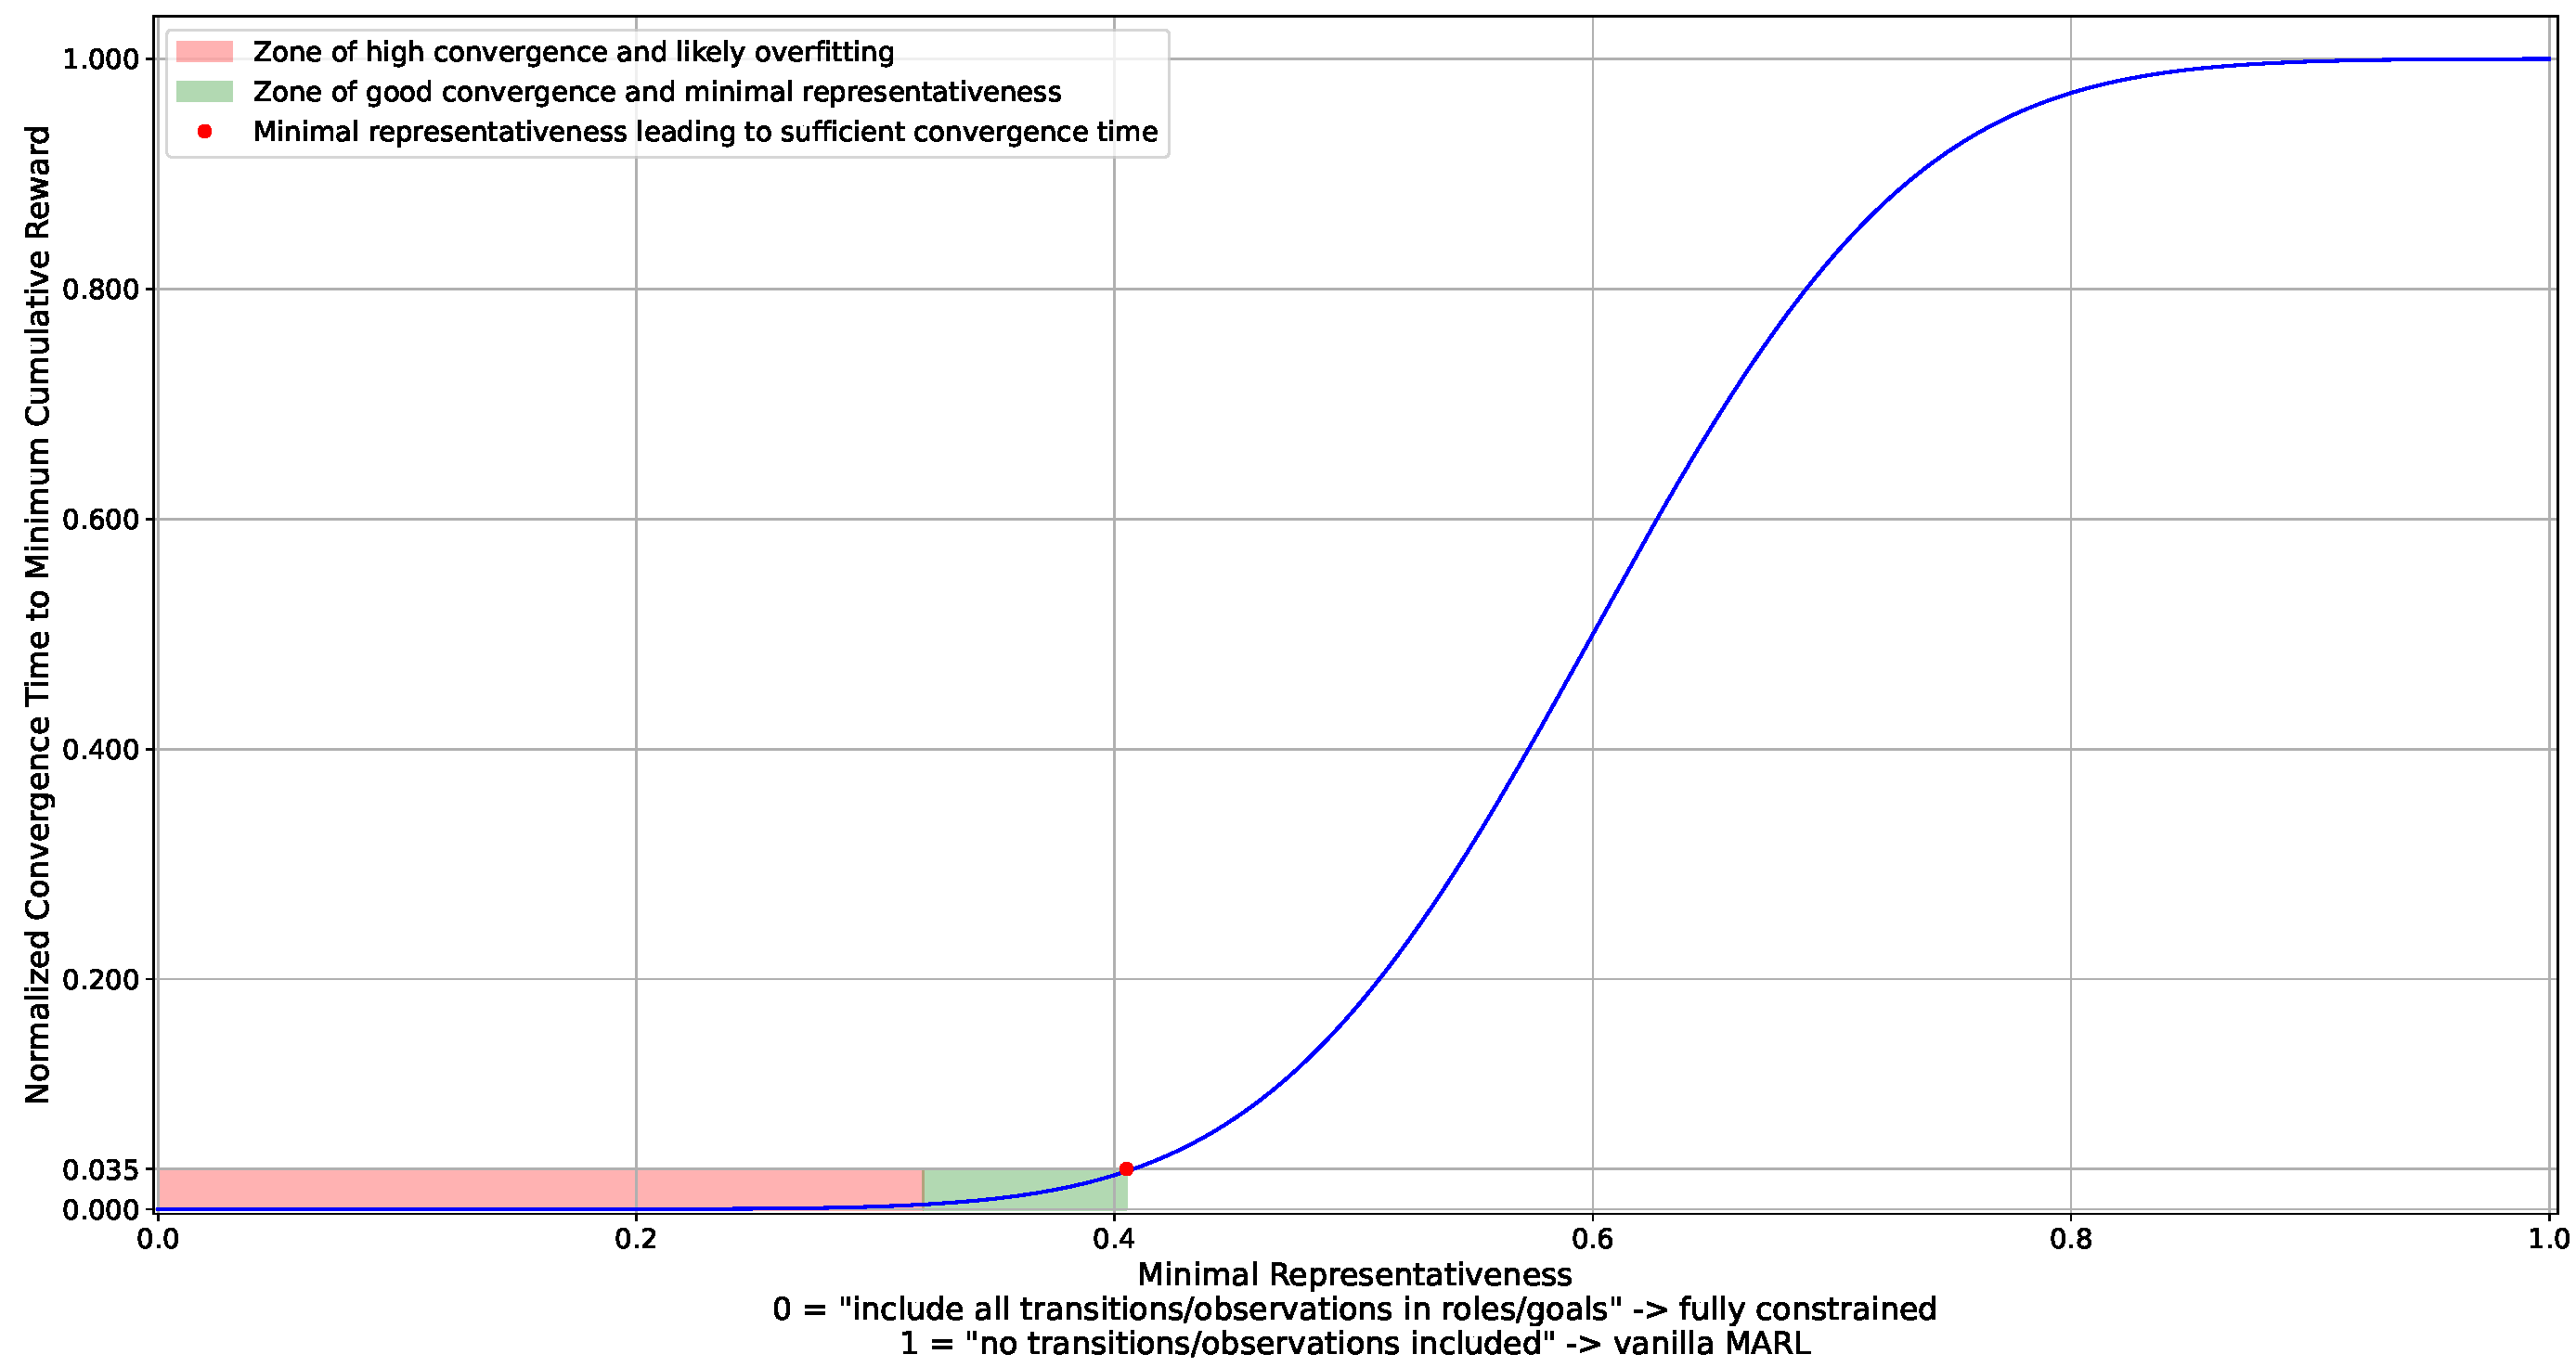
\includegraphics[trim=0cm 0cm 0cm 0cm, clip, width=1.\linewidth]{figures/convergence_time_relative_to_representativeness.pdf}
    \caption{Temps de convergence normalisé en fonction de la représentativité minimale}
    \label{fig:conv_time_repr}
\end{figure}




\section{Description et mise en oeuvre dans l'activité}

L’algorithme~\ref{alg:auto_temm} formalise le déroulement général de l’activité d’analyse.
Chaque étape est détaillée ci-dessous afin d’expliciter les mécanismes qui permettent d’inférer une spécification organisationnelle implicite et de calculer l’adéquation organisationnelle.

\paragraph{Étape 1 : Collecte des trajectoires.}
La première étape consiste à exécuter la politique conjointe $\pi^j$ dans l’environnement $d_\Omega$ afin de générer des historiques complets de transitions $(\omega, a, \omega')$.
Deux ensembles de données sont extraits :
\begin{itemize}
    \item $\mathcal{D}_{\text{trans}}$ contenant les séquences de transitions $(\omega_t, a_t, \omega_{t+1})$, utilisées pour l’inférence des rôles ;
    \item $\mathcal{D}_{\text{obs}}$ contenant uniquement les séquences d’observations $(\omega_t)$, utilisées pour l’inférence des objectifs et missions.
\end{itemize}

\paragraph{Étape 2 : Optimisation des distances et seuils de clustering.}
Pour réduire la variabilité entre trajectoires et identifier des structures récurrentes, les ensembles $\mathcal{D}_{\text{obs}}$ et $\mathcal{D}_{\text{trans}}$ sont soumis à un processus de clustering.
On explore plusieurs métriques de distance $\delta_t$ (ex. \acn{LCS}, Smith-Waterman, distances vectorielles) et seuils de regroupement $\tau_t$.
Chaque combinaison $(\delta_t, \tau_t)$ est évaluée selon un score pondérant :
\[
    \text{Score} = \alpha (\sigma_{\text{obs}} + \sigma_{\text{trans}}) + \beta N_{\text{clusters}}
\]
où $\sigma$ désigne la variance intra-cluster et $N_{\text{clusters}}$ le nombre total de clusters.
La combinaison minimisant ce score est retenue, garantissant un compromis entre cohérence interne et compacité des clusters.

\paragraph{Étape 3 : Application du clustering optimal.}
Une fois les hyperparamètres optimaux $(\delta^*, \tau^*)$ déterminés, les trajectoires sont regroupées :
\begin{itemize}
    \item les clusters de transitions $C_{trans}$ permettent d’inférer les \textbf{rôles} par extraction des séquences communes (\acn{CLS}) et des règles comportementales associées ;
    \item les clusters d’observations $C_{obs}$ servent à identifier les \textbf{objectifs intermédiaires} et les plans associés.
\end{itemize}

\paragraph{Étape 4 : Recherche de représentativité optimale.}
Le degré de représentativité $\rho_t$ fixe le seuil minimal pour qu’une transition ou observation soit retenue comme caractéristique d’un rôle ou objectif.
Une recherche par grille est effectuée sur différentes valeurs de $\rho_t$.
Pour chaque $\rho_t$, une spécification $\mathcal{MM}_{\rho_t}$ est inférée, puis une nouvelle politique $\pi^j_{\rho_t}$ est réentraînée dans $d_\Omega$.
On enregistre alors le temps de convergence $c_{\rho_t}$ pour atteindre une performance minimale $R_{\min}$.
Le paramètre optimal $\rho_t^*$ est choisi comme la plus grande représentativité garantissant une convergence inférieure au seuil $\eta$ (par défaut 3.5\%).

\paragraph{Étape 5 : Inférence finale des rôles et objectifs.}
Avec $(\delta^*, \tau^*, \rho^*)$, on extrait les rôles $\mathcal{R}$, les objectifs intermédiaires $\mathcal{G}$ et leurs relations hiérarchiques (missions, héritage de rôles).
Les permissions et obligations sont déduites en observant la systématicité (obligations) ou la variabilité (permissions) des associations rôle–mission dans les trajectoires.

\paragraph{Étape 6 : Calcul de l’adéquation organisationnelle.}
Deux indicateurs partiels sont calculés :
\begin{itemize}
    \item le \textbf{\acn{SOF}} (structural organizational fit), mesurant la cohérence des rôles via la variance des transitions intra-cluster ;
    \item le \textbf{\acn{FOF}} (functional organizational fit), mesurant la cohérence fonctionnelle dans l’atteinte des objectifs intermédiaires.
\end{itemize}
L’indicateur global est obtenu par agrégation :
\[
    \text{OF} = \frac{1}{2}(\text{SOF} + \text{FOF})
\]

\paragraph{Étape 7 : Sorties de l’activité.}
L’activité retourne :
\begin{itemize}
    \item une spécification implicite $\mathcal{MM}_{\text{implicit}}$ décrivant rôles, missions, permissions et obligations inférés automatiquement ;
    \item un score d’adéquation organisationnelle $\text{OF}$ permettant de quantifier la qualité organisationnelle des comportements émergents.
\end{itemize}


\begin{algorithm}[H]
    \caption{Algorithme de l'activité d'analyse}
    \label{alg:auto_temm}
    \DontPrintSemicolon

    \KwIn{
        Politique conjointe entraînée $\pi^j$~;
        \acn{ODec-POMDP} $d_\Omega$~;
        Spécification initiale $\mathcal{MM}$~;
        Seuil de convergence normalisé (défaut~: 3.5\%) $\eta$
    }

    \KwOut{
    Spécification organisationnelle inférée $\mathcal{MM}_{\text{implicit}}$~;
    Score de adéquation  organisationnel $\acn{OF}$
    }

    \tcp*[l]{1. Collecte des trajectoires}
    Générer les historiques individuels $\mathcal{D}_{\text{trans}}$ depuis $d_\Omega$ sous $\pi^j$ \;
    $\mathcal{D}_{\text{obs}} \gets$ trajectoires d'observations individuelles issues de $\mathcal{D}_{\text{full}}$ \;

    \tcp*[l]{2. \acn{HPO} sur distance et seuil de clustering}
    \For{$t \in \{obs, trans\}$}{
        \ForEach{métrique de distance $\delta_t$}{
            \ForEach{seuil minimal de cluster $\tau_t$}{
                Appliquer clustering avec $(\delta_t, \tau_t)$ \;
                Calculer $\sigma_{\text{obs}}, \sigma_{\text{trans}}, N_{\text{clusters}}$ \;
                Score $\gets \alpha (\sigma_{\text{obs}} + \sigma_{\text{trans}}) + \beta N_{\text{clusters}}$ \tcp*[l]{par défaut~: $\alpha=0.4$, $\beta=0.6$}
                Retenir $(\delta_t^*, \tau_t^*)$ avec Score minimal \;
            }
        }
    }

    \tcp*[l]{3. Application du clustering avec \acn{HPO} optimal}
    Clustering des observations~: $\mathcal{D}_{\text{obs}} \rightarrow C_{obs}$ via $(\delta_{obs}^*, \tau_{obs}^*)$ \;
    Clustering des transitions~: $\mathcal{D}_{\text{trans}} \rightarrow C_{trans}$ via $(\delta_{trans}^*, \tau_{trans}^*)$ \;

    \tcp*[l]{4. \acn{HPO} sur la représentativité (convergence)}
    \For{$t \in \{obs, trans\}$}{
    \ForEach{représentativité $\rho_t$}{
    Inférer $\mathcal{MM}_{\rho_t}$ à partir des clusters \;
    Initialiser une politique $\pi^j_{\rho_t}$ \;
    Entraîner $\pi^j_{\rho_t}$ sur $(d_\Omega, \mathcal{MM}_{\rho_t})$ jusqu'à atteindre $R_{\min}$ \;
    Enregistrer le temps de convergence $c_{\rho_t}$ tel que $ct_t(\rho_t) = c_{\rho_t}$ \;
    }

    \tcp*[l]{5. Sélectionner le point de coude}
    $\rho_t^* \gets max(\{\rho_t \ | \ ct_t(\rho_t) < \eta \})$ \tcp*[r]{par défaut $\eta = 3.5\%$}
    }

    \tcp*[l]{6. Inférence finale des rôles et objectifs}
    Inférer les rôles à partir de $\mathcal{D}_{\text{trans}}, \delta^*, \tau^*, \rho^*$ \;
    Inférer les objectifs à partir de $\mathcal{D}_{\text{obs}}, \delta^*, \tau^*, \rho^*$ \;

    \tcp*[l]{7. Calcul du adéquation  organisationnel}
    Calculer \acn{SOF} et \acn{FOF} à partir des variances intra-cluster \;
    $\text{OF} \gets \frac{1}{2}(\text{SOF} + \text{FOF})$ \;

    \Return{$\mathcal{MM}_{\text{implicit}}, \text{OF}$}
\end{algorithm}


\section{Synthèse}

En synthèse, l’activité d’analyse permet d’établir un lien objectif entre les comportements émergents des agents et les structures organisationnelles attendues. Grâce à la méthode \acn{TEMM} et à son extension Auto-\acn{TEMM}, il devient possible d’inférer automatiquement des rôles, objectifs et missions à partir des trajectoires, et de quantifier leur adéquation organisationnelle par un indicateur robuste. Cette démarche favorise l’explicabilité, la traçabilité et le raffinement itératif des spécifications organisationnelles, tout en fournissant des outils d’évaluation pour comparer différentes politiques ou configurations. Toutefois, la qualité de l’analyse dépend de la diversité des trajectoires collectées et du choix des hyperparamètres de clustering, même si l’automatisation par optimisation conjointe permet de limiter l’intervention humaine. Cette activité constitue ainsi un pivot essentiel pour la boucle de conception \acn{MAMAD}, en préparant le transfert et l’amélioration continue des politiques dans l’environnement réel.


\clearpage
\thispagestyle{empty}
\null
\newpage

\chapter{Transférer et superviser en environnement réel}
\label{chap:transferring}

L'\textit{activité de transfert} correspond à la mise en production et au suivi des politiques conjointes dans l’environnement réel.
Elle joue un double rôle : (i) assurer l’exécution continue de la politique la plus récente $\pi^j_{\text{latest}}$ dans $\mathcal{E}$, garantissant l’action efficace des agents, et (ii) collecter de nouvelles trajectoires réelles $(\omega^j_t, a^j_t, \omega^j_{t+1})$ pour enrichir la base de données $\mathcal{D}_{H^j}$, permettant la mise à jour du modèle simulé et des spécifications organisationnelles.

\section*{Objectifs formels}

Les \textbf{entrées} de l’activité de transfert sont :
\begin{itemize}
    \item la politique conjointe la plus récente $\pi^j_{\text{latest}}$ ;
    \item l’environnement réel $\mathcal{E}$ ;
    \item la base de trajectoires accumulées $\mathcal{D}_{H^j}$.
\end{itemize}

Les \textbf{sorties attendues} sont :
\begin{itemize}
    \item une base enrichie de trajectoires $\mathcal{D}_{H^j}$ ;
    \item un signal $\texttt{need\_update}$ déclenchant la reprise du cycle de conception.
\end{itemize}

La relation globale peut être exprimée par :
\[
    \mathcal{D}_{H^j}, \texttt{need\_update} \gets \texttt{transfer}(\pi^j_{\text{latest}}, \mathcal{E}, \mathcal{D}_{H^j})
\]

\section{Travaux mobilisés et verrous identifiés}

L’activité de transfert et de supervision en environnement réel s’appuie sur plusieurs axes : le transfert de politiques (policy transfer), l’adaptation de domaine (sim2real), la calibration dynamique des modèles (online model calibration), et la supervision continue des systèmes multi-agents.

Les approches de \textit{Robust Reinforcement Learning}~\cite{pinto2017robust} visent à rendre les politiques résistantes aux écarts simulation/réalité, mais n’intègrent pas la mise à jour du modèle simulé après déploiement. Les méthodes d’adaptation de domaine et \textit{Sim2Real}~\cite{tobin2017domain,ganin2016domain} réduisent l’écart simulation/réel via la randomisation ou l’apprentissage de représentations invariantes, mais leur adaptation en ligne reste limitée. Les techniques de calibration dynamique~\cite{deisenroth2011pilco} mettent à jour le modèle simulé à partir des retours du réel, sans prise en compte explicite de l’adaptation des politiques multi-agents. Enfin, la synchronisation manuelle reste courante mais peu adaptée aux environnements dynamiques.

Les principaux verrous sont :
\begin{itemize}
    \item l’absence de cadre unifié pour la mise à jour conjointe du modèle simulé et des politiques déployées ;
    \item la difficulté à détecter et corriger automatiquement les écarts simulation/réalité ;
    \item le manque de mécanismes intégrés pour garantir robustesse et sécurité lors du transfert ;
    \item la nécessité d’une supervision continue et automatisée.
\end{itemize}

Ces limites motivent le développement d’un cadre méthodologique assurant l’adaptation conjointe du jumeau numérique et des politiques multi-agents, avec supervision automatisée du transfert.

\section{Positionnement et contributions proposées}

L’approche proposée introduit un \textbf{cadre de transfert asynchrone et événementiel} comprenant :
\begin{itemize}
    \item une \textbf{Boucle de transfert} (\texttt{Transfer Loop}) qui assure l’exécution en continu de la politique et la collecte des trajectoires dans un tampon temporaire $\mathcal{B}$ ;
    \item un \textbf{Déclencheur de mise à jour} (\texttt{Update Trigger}) qui ajoute les trajectoires à la base $\mathcal{D}_{H^j}$ et active, de façon asynchrone, les activités de modélisation et d’entraînement dès qu’un seuil $\texttt{batch\_size}$ est atteint.
\end{itemize}

Ce double mécanisme assure la continuité du fonctionnement des agents, tout en maintenant la boucle de conception synchronisée avec les données réelles.

\section{Description et mise en œuvre de l’activité}

L’algorithme~\ref{alg:transferring} formalise le fonctionnement de l’activité de transfert.
Chaque élément est décrit ci-dessous afin de préciser les mécanismes et leur rôle dans la boucle de conception.

\paragraph{Entrées et sorties.}
L’activité reçoit en entrée :
\begin{itemize}
    \item la politique conjointe la plus récente $\pi^j_{\text{latest}}$, produite lors de l’entraînement ;
    \item l’environnement réel $\mathcal{E}$, représentant le domaine opérationnel où le \acn{SMA} agit ;
    \item la base courante de trajectoires $\mathcal{D}_{H^j}$, enrichie au fil des déploiements.
\end{itemize}
En sortie, elle retourne :
\begin{itemize}
    \item une base de trajectoires mise à jour $\mathcal{D}_{H^j}$ ;
    \item un signal booléen $\texttt{need\_update}$ indiquant si les activités de modélisation et d’entraînement doivent être relancées.
\end{itemize}

\paragraph{Boucle de transfert.}
La boucle de transfert s’exécute tant que le \acn{SMA} est actif dans $\mathcal{E}$.
À chaque pas de temps $t$ :
\begin{enumerate}
    \item une observation $\omega^j_t$ est collectée via la fonction $\texttt{observe}(\mathcal{E})$ ;
    \item l’action $a^j_t$ est choisie en appliquant la politique $\pi^j_{\text{latest}}$ à l’observation courante ;
    \item cette action est exécutée dans l’environnement via $\texttt{apply}(\mathcal{E}, a^j_t)$, produisant la nouvelle observation $\omega^j_{t+1}$ ;
    \item la transition $(\omega^j_t, a^j_t, \omega^j_{t+1})$ est stockée dans un tampon temporaire $\mathcal{B}$.
\end{enumerate}

\paragraph{Déclencheur de mise à jour.}
Lorsque la taille du tampon $\mathcal{B}$ dépasse un seuil $\texttt{batch\_size}$, le contenu est ajouté à la base de trajectoires $\mathcal{D}_{H^j}$ puis le tampon est vidé.
Le signal $\texttt{need\_update}$ est alors activé.
Si aucun processus de mise à jour n’est en cours (\texttt{not running\_update}), la procédure \texttt{launch\_update()} est déclenchée de manière asynchrone pour relancer les activités de modélisation et d’entraînement.

\paragraph{Fonctionnement global.}
Ce schéma assure trois propriétés essentielles :
\begin{itemize}
    \item la \textbf{continuité d’exécution} : les agents opèrent toujours avec la dernière politique disponible ;
    \item la \textbf{réactivité} : les données réelles sont intégrées dès qu’un volume suffisant est collecté ;
    \item la \textbf{automatisation} : les mises à jour se déclenchent sans intervention humaine, tout en évitant les conflits entre processus parallèles.
\end{itemize}

\paragraph{Éléments formels.}
Ainsi, l’algorithme encode la relation :
\[
    \mathcal{D}_{H^j}, \texttt{need\_update} \gets \texttt{transfer}(\pi^j_{\text{latest}}, \mathcal{E}, \mathcal{D}_{H^j})
\]
où :
\begin{itemize}
    \item $\mathcal{B}$ désigne le tampon temporaire,
    \item $\texttt{batch\_size}$ fixe la granularité de déclenchement des mises à jour,
    \item $\texttt{launch\_update}()$ assure la synchronisation avec les autres activités de la méthode \acn{MAMAD}.
\end{itemize}

\vspace{-0.3em}
\begin{algorithm}[H]
    \caption{Activité de transfert}
    \label{alg:transferring}
    \DontPrintSemicolon
    \KwIn{Politique actuelle $\pi^j_{\text{latest}}$, environnement réel $\mathcal{E}$, base de trajectoires $\mathcal{D}_{H^j}$}
    \KwOut{Base de trajectoires mise à jour $\mathcal{D}_{H^j}$, signal de mise à jour $\texttt{need\_update}$}

    \vspace{0.3em}
    \SetKwProg{Transfer}{Procédure \normalfont BoucleDeTransfert}{}{}
    \Transfer{}{

    \While{le \acn{SMA} est actif dans l'environnement $\mathcal{E}$}{
    \tcp*[l]{Exécution de la politique la plus récente}
    $\omega^j_t \gets \texttt{observe}(\mathcal{E})$ \;
    $a^j_t \gets \pi^j_{\text{latest}}(\omega^j_t)$ \;
    $\omega^j_{t+1} \gets \texttt{apply}(\mathcal{E}, a^j_t)$ \;
    Ajouter $(\omega^j_t, a^j_t, \omega^j_{t+1})$ au tampon temporaire $\mathcal{B}$ \;

    \tcp*[l]{Vérification du déclenchement de la mise à jour}
    \If{$|\mathcal{B}| \geq \texttt{batch\_size}$}{
        Ajouter $\mathcal{B}$ à $\mathcal{D}_{H^j}$ et vider $\mathcal{B}$ \;
        $\texttt{need\_update} \gets \texttt{True}$ \;
        \If{$\texttt{not running\_update} = \texttt{False}$}{
            \texttt{launch\_update()} \tcp*[r]{Appel asynchrone}
        }
    }
    }
    }
\end{algorithm}


\section{Synthèse}

En synthèse, l’activité de transfert assure l’exécution continue de la politique la plus récente et la collecte automatisée de trajectoires réelles pour raffiner le modèle et réentraîner les politiques.

Ses atouts sont :
\begin{itemize}
    \item automatisation du déploiement et de la collecte en environnement réel ;
    \item synchronisation robuste avec les autres activités de \acn{MAMAD} ;
    \item adaptation continue des agents à l’environnement.
\end{itemize}

Ses limites portent sur le coût de supervision, la gestion des environnements critiques, et la fréquence optimale des mises à jour.

Cette activité permet une méthode réellement \textbf{autoadaptative}, alternant apprentissage simulé et déploiement réel pour garantir la robustesse des \acn{SMA} en contexte dynamique.



\clearpage
\thispagestyle{empty}
\null
\newpage

\chapter*{Conclusion}
\addcontentsline{toc}{chapter}{\textbf{Conclusion}}

\noindent
Cette troisième partie a introduit la méthode \textbf{\acn{MAMAD}} comme une réponse concrète aux limites identifiées dans les approches actuelles de conception de \acn{SMA}. Reposant sur un cycle itératif structuré en quatre activités (\textit{Modélisation}, \textit{Apprentissage}, \textit{Analyse}, \textit{Transfert}), \acn{MAMAD} articule de manière cohérente des outils symboliques (spécifications organisationnelles) et \acn{MARL} pour guider la conception, l'entraînement et l'adaptation d'agents intelligents dans des environnements complexes.

\medskip

\noindent
La méthode s'appuie notamment~:
\begin{itemize}
    \item sur une modélisation fidèle des environnements à partir de données empiriques,
    \item sur un entraînement contraint par des spécifications organisationnelles intégrées au sein du cadre \textit{MOISE+MARL},
    \item sur une analyse des trajectoires pour inférer les structures émergentes de l'organisation apprise,
    \item et enfin sur un transfert contrôlé permettant l'amélioration itérative du \acn{SMA}.
\end{itemize}

\noindent
Dans la partie suivante, nous proposons de valider expérimentalement cette méthode à travers son implémentation concrète dans un outil dédié, \acn{CybMASDE}, et son application à plusieurs environnements représentatifs. L'objectif est de démontrer la capacité de \acn{MAMAD} à produire automatiquement des \acplu{SMA} performants, explicables et conformes à des exigences organisationnelles dans des contextes variés.

\medskip

\noindent
Nous évaluons notamment la méthode selon des critères d'efficacité, d'automatisation, de conformité aux contraintes et d'explicabilité, tout en comparant ses résultats à ceux d'approches classiques non guidées par des modèles organisationnels.

\bigskip

La \autoref{part:experimentation} met donc à l'épreuve la méthode \acn{MAMAD}, en analysant ses performances et sa pertinence au regard des verrous identifiés sur différents scénarios.

\clearpage
\thispagestyle{empty}
\null
\newpage

\cleardoublepage
\phantomsection
% \pdfbookmark[1]{Experimental validation of the method}{Experimental validation of the method}
\markboth{\textsc{Experimental validation of the method}}{\textsc{Experimental validation of the method}}
\part{Experimental validation of the method}
\label{part:experimentation}

\clearpage
\thispagestyle{empty}
\null
\newpage

% \acn{TODO}:
% - In the chapter on CybMASDE, start by giving a general overview of the platform (screenshots, activity diagram), its architecture (\acn{UML}: sequence, class, component) and the technical choices made (hyperparameter values).
% - For the chapter on the experimentation protocol, include the table linking each criterion to a set of metrics. The idea is to establish a common evaluation grid for the six different environments in order to verify or see how the set of criteria (C1 to C5) are valid for each environment tested according to the different baselines. The rest of the protocol must include elements such as hardware and software configuration, the different baselines (with or without organizational specifications, changing the severity of constraints, training frequency, etc. \acn{TODO}: but to be defined completely).
% - For the next chapter, we can keep the description of each environment (including observations, actions, states, rewards, etc.), briefly recalling the specific application of the protocol for that environment.
% - For the next chapter, we can present the results and how, according to the evaluation grid (based on the metrics) of the experimental protocol, the criteria are covered. At the end, we can provide a general summary of the results using the common evaluation grid (since we have numerical values, we can calculate averages, study standard deviations, etc.). This allows us to see, in general terms, how our applied method consistently and broadly covers all of the criteria.


\chapter*{Introduction}
\addcontentsline{toc}{chapter}{\textbf{Introduction}}

\noindent
This section aims to demonstrate the applicability and relevance of the \acn{MAMAD} method in all or part of its activities in different \acplu{SMA} design contexts . To this end, we have developed a dedicated platform, \acn{CybMASDE}, which implements the entire proposed pipeline (modeling, learning, analysis, transfer) in a modular and reproducible manner.

\medskip

\noindent
First, we describe in detail the experimental environment, the software and hardware tools used, and the test environments selected. We also present the organizational specifications associated with each environment, as well as the evaluation metrics used to validate the method's performance. \autoref{fig:organisation_manuscript_part_4} illustrates the organization of this section.

\medskip

\noindent
Second, we analyze the results obtained in order to meet the research objectives identified in the previous section. This includes an evaluation of the method's effectiveness, its capacity for automation, the adequacy of the learned policies with respect to organizational constraints, and their explainability.

\medskip

\noindent
This experimental study will enable us to better understand the strengths and limitations of the \acn{MAMAD} method and to identify opportunities for improvement for even greater automation of organizational design in \acn{MARL}.

\begin{figure}[h!]
  \centering
  \resizebox{0.7\linewidth}{!}{%
    \begin{tikzpicture}[
        chapter/.style={draw, fill=blue!10, thick, minimum width=9cm, minimum height=1.2cm, text centered, font=\bfseries},
        section/.style={draw, fill=blue!5, thick, minimum width=8cm, minimum height=1cm, text centered, font=\small},
        arrow/.style={-Latex, thick},
        node distance=0.4cm,
        annotated/.style={above,font=\small\itshape, inner sep=1pt, yshift=0.8cm, xshift=-8cm}
    ]

    % Chapitre 11 : Implémentation et outils
    \node[chapter] (ch11) {\parbox{10cm}{Chapitre 11 : CybMASDE : Un framework supportant MAMAD}};
    \node[section, below=1cm of ch11, xshift=-2cm] (ch11s1) {Intégration des différentes contributions};

    \draw[arrow] ($ (ch11.south) + (4.0,0) $) -- ++(0,0) |- (ch11s1.east) node[annotated] {Architecture logicielle modulaire au cœur du framework.};

    % Chapitre 12 : Cadre expérimental
    \node[chapter, below=1cm of ch11s1, xshift=2cm] (ch12) {\parbox{10cm}{Chapitre 12 : Cadre expérimental et d'évaluation}};
    \node[section, below=1cm of ch12, xshift=-2cm] (ch12s1) {Description des ensembles d'environnements et d'algorithmes considérés};
    \node[section, below=1cm of ch12s1] (ch12s2) {Conditions de reproductibilité};
    \node[section, below=1cm of ch12s2] (ch12s3) {Baselines expérimentales};
    \node[section, below=1cm of ch12s3] (ch12s4) {Grille d'évaluation};
    \node[section, below=1cm of ch12s4] (ch12s5) {Protocole d'experimentation et d'évaluation};

    \draw[arrow] ($ (ch12.south) + (4.0,0) $) -- ++(0,0) |- (ch12s1.east) node[annotated] {Définition des briques fondatrices pour l'experimentation.};
    \draw[arrow] ($ (ch12.south) + (4.0,0) $) -- ++(0,0) |- (ch12s2.east) node[annotated] {Résumé des conditions de reproduction expérimentales};
    \draw[arrow] ($ (ch12.south) + (4.0,0) $) -- ++(0,0) |- (ch12s3.east) node[annotated] {Définition les différentes expérimentations};
    \draw[arrow] ($ (ch12.south) + (4.0,0) $) -- ++(0,0) |- (ch12s4.east) node[annotated] {Définition un cadre commun pour l'évaluation};
    \draw[arrow] ($ (ch12.south) + (4.0,0) $) -- ++(0,0) |- (ch12s5.east) node[annotated] {Assemblage des éléments pour définir un protocole};

    % Chapitre 13 : Études de cas
    \node[chapter, below=1cm of ch12s5, xshift=2cm] (ch13) {\parbox{10cm}{Chapitre 13 : Études de cas}};
    \node[section, below=1cm of ch13, xshift=-2cm] (ch13s1) {Expérimentations sur les environnements non-orientés Cyberdéfense};
    \node[section, below=1cm of ch13s1] (ch13s2) {Expérimentations sur l'environnement Company infrastructure};
    \node[section, below=1cm of ch13s2] (ch13s3) {Expérimentations sur l'environnement Microservices Kubernetes};
    \node[section, below=1cm of ch13s3] (ch13s4) {Expérimentations sur l'environnement Drone Swarm};

    \draw[arrow] ($ (ch13.south) + (4.0,0) $) -- ++(0,0) |- (ch13s1.east) node[annotated] {};
    \draw[arrow] ($ (ch13.south) + (4.0,0) $) -- ++(0,0) |- (ch13s2.east) node[annotated] {};
    \draw[arrow] ($ (ch13.south) + (4.0,0) $) -- ++(0,0) |- (ch13s3.east) node[annotated] {};
    \draw[arrow] ($ (ch13.south) + (4.0,0) $) -- ++(0,0) |- (ch13s4.east) node[annotated] {};

    % Chapitre 14 : Résultats et synthèse
    \node[chapter, below=1cm of ch13s4, xshift=2cm] (ch14) {\parbox{10cm}{Chapitre 14 : Résultats expérimentaux et analyse}};
    \node[section, below=1cm of ch14, xshift=-2cm] (ch14s1) {Résultats et discussion des environnements non-orientés Cyberdéfense};
    \node[section, below=1cm of ch14s1] (ch14s2) {Résultats et discussion de l'environnement Company Infrastructure};
    \node[section, below=1cm of ch14s2] (ch14s3) {Résultats et discussion de l'environnement Microservices Kubernetes};
    \node[section, below=1cm of ch14s3] (ch14s4) {Résultats et discussion de l'environnement Drone Swarm};

    \draw[arrow] ($ (ch14.south) + (4.0,0) $) -- ++(0,0) |- (ch14s1.east) node[annotated] {};
    \draw[arrow] ($ (ch14.south) + (4.0,0) $) -- ++(0,0) |- (ch14s2.east) node[annotated] {};
    \draw[arrow] ($ (ch14.south) + (4.0,0) $) -- ++(0,0) |- (ch14s3.east) node[annotated] {};
    \draw[arrow] ($ (ch14.south) + (4.0,0) $) -- ++(0,0) |- (ch14s4.east) node[annotated] {};

    % Transitions entre chapitres
    \draw[arrow] ($ (ch11.south) + (4.5,0) $) -- ($ (ch12.north) + (4.5,0) $) node[annotated, yshift=-0.5cm] {L'outil étant en place, nous définissons le protocole pour l'évaluer.};
    \draw[arrow] ($ (ch12.south) + (4.5,0) $) -- ($ (ch13.north) + (4.5,0) $) node[annotated, yshift=-0.5cm] {Le protocole est appliqué à différents environnements.};
    \draw[arrow] ($ (ch13.south) + (4.5,0) $) -- ($ (ch14.north) + (4.5,0) $) node[annotated, yshift=-0.5cm] {Les résultats sont analysés pour valider la méthode.};

\end{tikzpicture}

  }
  \caption{Structure of Part IV: Experimental framework and analysis of results}
  \label{fig:organisation_manuscript_part_4}
\end{figure}

\clearpage
\thispagestyle{empty}
\null
\newpage

\chapter{CybMASDE: A framework supporting MAMAD}
\label{sec:cybmasde}

% 1 - Introduction
% 2 - Features
% 3 - Internal architecture
% 4 - Implementation
% 5 - Illustrative scenario

\acn{CybMASDE}\footnotemark[1] is a modular and extensible platform that we propose to support the \acn{MAMAD} method. It integrates all the implementations of the contributions proposed in the method in order to meet the various expectations of the designer.
It allows designers to model the target environment, determine effective policies, and then analyze them to infer understandable organizational specifications by alternating between training and analysis. At the same time, \acn{CybMASDE} maintains consistency between the simulated environment and the real environment by updating both the simulated model and the deployed policies.
%
\acn{CybMASDE} can be used primarily in \acn{CLI} mode with the \textquote{cybmasde} command (see the manual in \autoref{appendix:cybmasde-manual}), but also offers a graphical interface for performing the main configuration tasks.


\section{Features offered by $\texttt{CybMASDE}$}

This section describes the typical journey of a \acn{CybMASDE} user, from modeling the environment to obtaining a satisfactory joint policy accompanied by performance measures, stability, and explanatory organizational specifications. Each step indicates both the user's actions and the platform's internal processes.

In general, the \textbf{Designer} can activate any feature as long as the dependencies between features are respected.
% (see \autoref{fig:cybmasde_usecase}).
For example, it is possible to start training if the environment has been previously modeled manually.

% \begin{figure}[h!]
% \centering
% 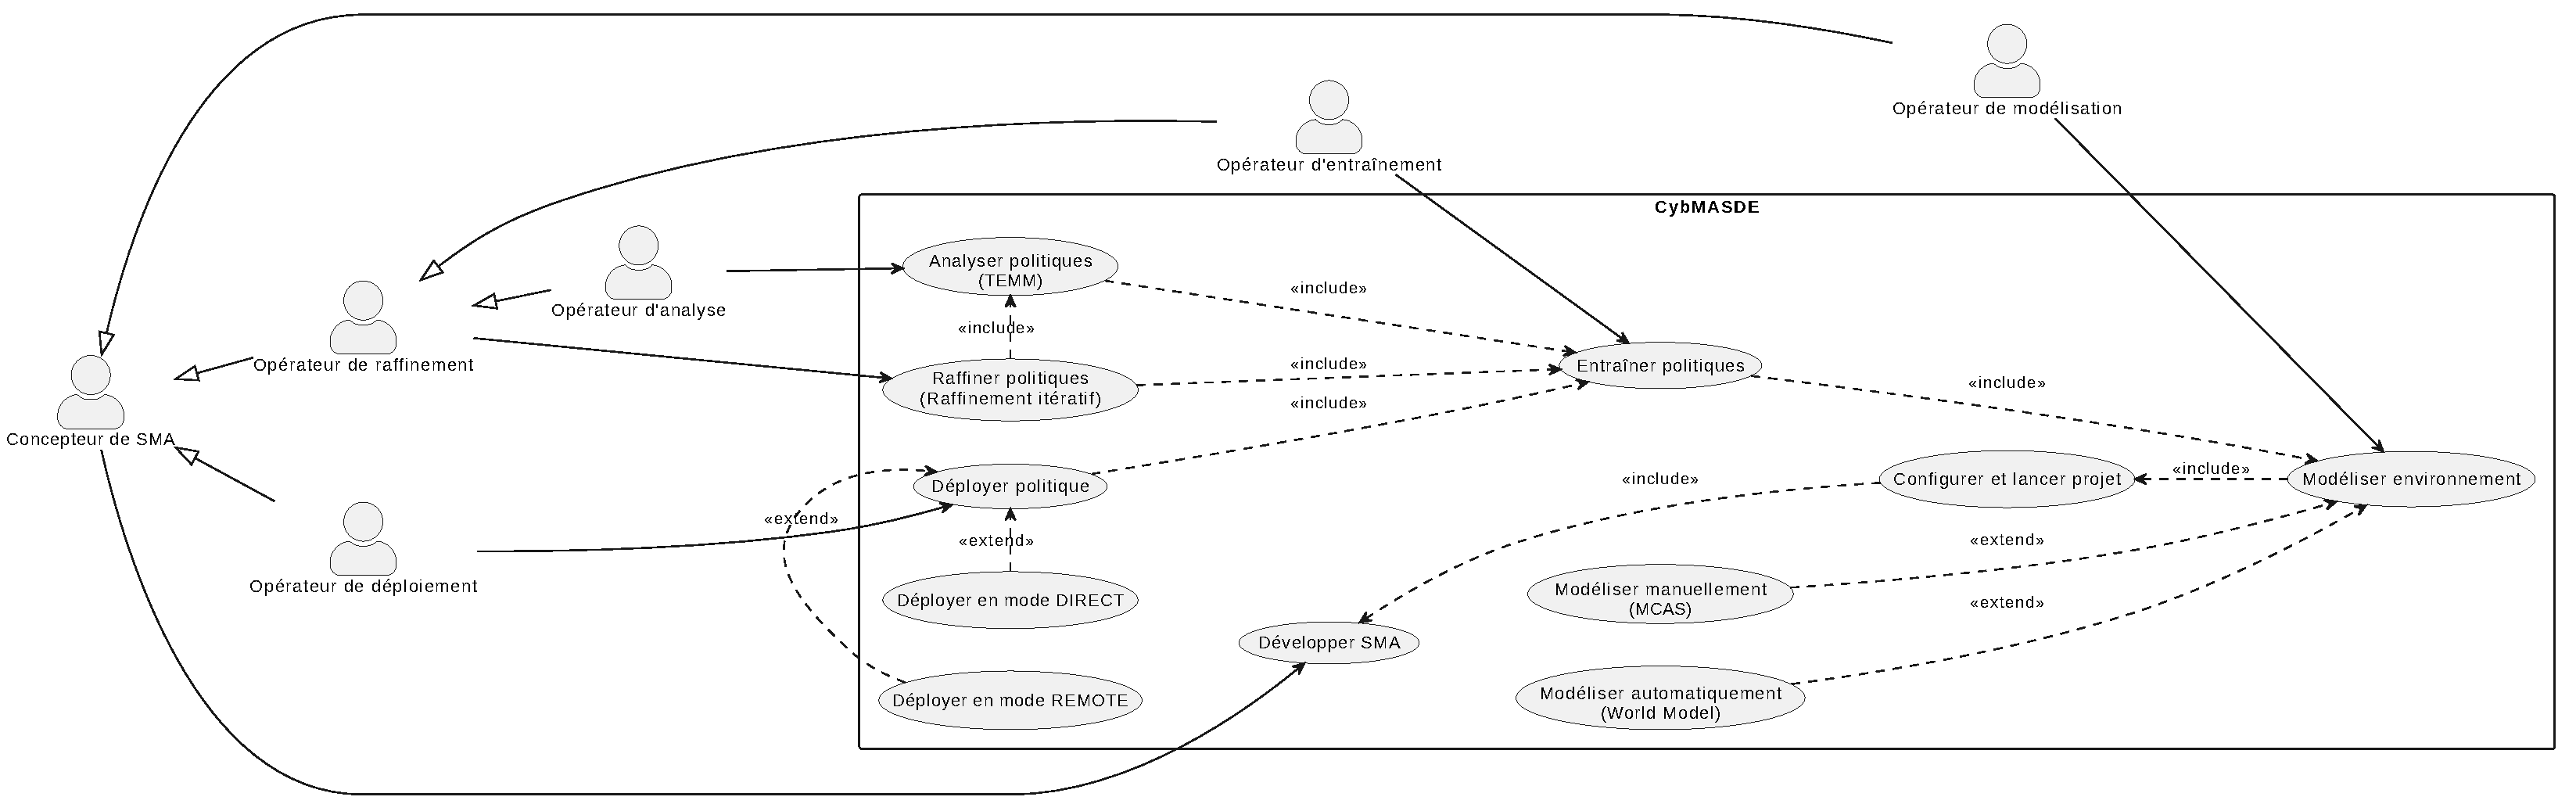
\includegraphics[width=\linewidth]{figures/use_case_cybmasde.pdf}
% \caption{CybMASDE use case diagram}
% \label{fig:cybmasde_usecase}
% \end{figure}

Although the \textbf{Designer} represents the \textquote{general} role, they actually play different roles when interacting with \acn{CybMASDE}~:
\begin{itemize}
  \item \textbf{Environment modeler}, responsible for defining or completing the description of the simulated environment, either automatically using a \textbf{World Model}, or manually using the \acn{MCAS} model;
  \item \textbf{Agent trainer}, who conducts the learning phases of multi-agent policies, taking into account organizational specifications;
  \item \textbf{Organizational analyst}, who uses the \acn{TEMM} or \acn{Auto-TEMM} method to infer organizational roles and objectives from the trajectories produced;
  \item \textbf{Specification refiner}, which combines the two previous roles to perform iterative training and analysis cycles until a satisfactory policy is obtained~;
  \item \textbf{Deployment operator}, which supervises the integration of the final joint policy into the real environment, either in \textit{DIRECT} mode (policy executed locally by agents) or in \textit{REMOTE} mode (policy executed by the \textit{Transferring} process).
\end{itemize}

In practice, \acn{CybMASDE} is designed as a tool that can mainly be used in \acn{CLI} mode: each step of the \acn{MAMAD} cycle (Modeling, Training, Analyzing, Transferring) is exposed through an explicit command.
%
After creating a new project, \acn{CybMASDE} automatically generates a folder tree structured around the four main activities of the \acn{MAMAD} method (modeling, training, analysis, transfer), as well as a central configuration file $\texttt{project\_configuration.json}$. A detailed example of this file for the Overcooked-AI environment is given in \autoref{tab:cybmasde_config}.

\begin{table}[h!]
    \centering
    \caption{Résumé du fichier \textquote{project\_configuration.json} avec exemples sur Overcooked-AI}
    \tiny
    \renewcommand{\arraystretch}{1.4}
    \label{tab:cybmasde_config}
    \begin{tabularx}{\linewidth}{
            >{\raggedright\arraybackslash\hsize=0.2\hsize}X
            >{\raggedright\arraybackslash\hsize=0.4\hsize}X
            >{\raggedright\arraybackslash\hsize=0.4\hsize}X}
        \hline
        \textbf{Clé / Élément}                                                                      & \textbf{Rôle dans CybMASDE}                                              & \textbf{Exemple (Overcooked-AI)}                                        \\
        \hline
        \textquote{common . project\_name}                                                          & Nom du projet                                                            & \textquote{"Overcooked\_coop"}                                          \\
        \hline
        \textquote{common . project\_description}                                                   & Brève description du projet                                              & \textquote{"Test coopération à 2 agents"}                               \\
        \hline
        \textquote{common . label\_manager}                                                         & Fichier Python mappant actions/observations en étiquettes                & Associer \textquote{0→move\_north}, \textquote{1→pickup\_onion}         \\
        \hline
        \textquote{common . project\_path}                                                          & Chemin absolu du projet                                                  & \textquote{/home/user/Overcooked\_coop}                                 \\
        \hline
        \textquote{modelling . simulated\_environment . environment\_path}                          & Environnement manuel (MCAS) si utilisé                                   & Vide si World Model uniquement                                          \\
        \hline
        \textquote{modelling . generated\_environment . world\_model . jopm . autoencoder}          & Encodeur d’observations (VAE)                                            & VAE compressant la cuisine en vecteur latent (dim=32)                   \\
        \hline
        \textquote{modelling . generated\_environment . world\_model . jopm . rdlm}                 & Modèle dynamique (RNN+MLP)                                               & Prédit transition après action \textquote{pickup\_onion}                \\
        \hline
        \textquote{modelling . generated\_environment . world\_model . initial\_joint\_observation} & Observations initiales                                                   & Positions des 2 cuisiniers et des ingrédients                           \\
        \hline
        \textquote{modelling . generated\_environment . component\_functions\_path}                 & Fonctions \textquote{reward()}, \textquote{stop()}, \textquote{render()} & \textquote{reward=+1} si soupe servie ; \textquote{stop} après 400 pas  \\
        \hline
        \textquote{modelling . organizational\_specifications}                                      & Spécifications MOISE+MARL                                                & Rôles \textquote{Chef1}, \textquote{Chef2}, missions : ramasser, servir \\
        \hline
        \textquote{training . hyperparameters}                                                      & Paramètres MARL                                                          & \textquote{lr=0 . 0003}, \textquote{gamma=0 . 95}, batch=128            \\
        \hline
        \textquote{training . statistics}                                                           & Résultats d’entraînement                                                 & Récompense moyenne par épisode                                          \\
        \hline
        \textquote{training . joint\_policy}                                                        & Dernier checkpoint de la politique conjointe                             & \textquote{policy\_epoch200 . pth}                                      \\
        \hline
        \textquote{analyzing . hyperparameters}                                                     & Paramètres Auto-TEMM                                                     & Distance DTW, seuil représentativité=0 . 3                              \\
        \hline
        \textquote{analyzing . statistics}                                                          & Résultats quantitatifs                                                   & Variance des récompenses = 0 . 12                                       \\
        \hline
        \textquote{analyzing . figures\_path}                                                       & Graphiques produits                                                      & Dendrogrammes de rôles, courbes de convergence                          \\
        \hline
        \textquote{analyzing . post\_training\_trajectories\_path}                                  & Trajectoires utilisées pour l’analyse                                    & Séquence d’actions collectives pour une soupe                           \\
        \hline
        \textquote{analyzing . inferred\_organizational\_specifications}                            & Spécifications MOISE+MARL inférées                                       & Agent A spécialisé en ramassage, Agent B en service                     \\
        \hline
        \textquote{transferring . last\_checkpoint}                                                 & Politique finale à déployer                                              & \textquote{policy\_final . pth}                                         \\
        \hline
        \textquote{transferring . configuration}                                                    & Paramètres de transfert (mode, API)                                      & \textquote{"mode": "REMOTE", "api\_url": "http://localhost:8000"}       \\
        \hline
    \end{tabularx}
\end{table}


The general principle of \acn{CybMASDE} is that the user must invest a significant initial effort to configure all the parameters of their project, centralized in the \texttt {project\_configuration.json}.
The designer then enters the necessary information for each activity, mainly in the form of Python code, JSON, or by specifying the paths to existing files. For example, for modeling, the user can provide the path to an existing simulation, or choose to create a new one by defining the space of observations, actions, reward, stop, and possibly rendering functions based on history, as well as the hyperparameters for training the World Model.
Once this preparatory work has been completed, the entire pipeline becomes automatable and no longer necessarily requires manual intervention except for refinement cycles.

\medskip

\noindent The typical path for the command lines entered is generally as follows:
\begin{enumerate}
  \item \textbf{$\texttt{init}$}: creates the project tree and a blank configuration file.
        The user then completes this file by filling in the observation and action spaces, reward and stop functions, organizational specifications, and training hyperparameters. A required step for configuration is to implement an \textbf{Environmental API} by implementing the \textquote{environment\_api} interface, which will allow \acn{CybMASDE} to communicate with the target environment (see \autoref{appendix:cybmasde-environment-api}).
  \item \textbf{$\texttt{validate}$}: checks the completeness and consistency of the project.
        In case of errors (missing file, unimplemented function, invalid API), execution is stopped with an explicit message.
  \item \textbf{$\texttt{model}$}: models a simulated environment from the real environment.
        Two variants exist:
        $\texttt{model --auto}$, which triggers the generation of a World Model from traces, and
        $\texttt{model --manual}$, which loads an instance \acn{MCAS} filled in by the user.
  \item \textbf{$\texttt{train --algo <alg>}$}: trains multi-agent policies using the algorithms available in MARLlib (MAPPO, MADDPG, QMix, etc.).
        Training automatically applies the organizational constraints defined in the project.
  \item \textbf{$\texttt{analyze --auto-temm}$}: applies the Auto-TEMM method to extract organizational specifications (roles, objectives) and organizational fit metrics.
        The results are saved in the $\texttt{analyzing/}$ folder.
  \item \textbf{$\texttt{refine --max <N>}$}: launches an iterative loop combining training and analysis until a satisfactory joint policy is obtained (reward and stability thresholds reached, or manual stop by the user).
  \item \textbf{$\texttt{deploy}$}: deploys the validated joint policy in the real environment, either in $\texttt{--direct}$ mode (agents execute the policy autonomously) or in $\texttt{--remote}$ mode (the \textit{Transferring} process executes the policy and sends the actions).
  \item \textbf{Utility commands}:
        $\texttt{run --full-auto}$ (complete execution of the pipeline without interruption),
        $\texttt{run --manual}$ (step-by-step execution),
        $\texttt{status}$ (monitoring of a project in progress),
        $\texttt{export --format <fmt>}$ (export results and metrics),
        $\texttt{clean --all}$ (reset the working environment).
\end{enumerate}

\medskip
\noindent

\paragraph{Typical example of use in automatic mode.}
A common scenario for using \acn{CybMASDE} is to execute the entire \textbf{MTA+T} pipeline (\textit{Modeling}, \textit{Training}, \textit{Analyzing}, \textit{Transferring}) in fully automated mode, for example during reproducible experiments on a computing cluster.
In this case, a single command line is sufficient to orchestrate all the steps, without any human interaction, as illustrated below:

\begin{lstlisting}[language=bash, caption={Complete execution of CybMASDE in full-auto mode}, label={lst:cybmasde_full_auto}]
cybmasde run \
--full-auto \ # complete pipeline (MTA+T) without interaction
--project /home/john/Documents/new_test \ # path to the project
--config /home/john/Documents/new_test/project\_configuration.json \ # config file
--max-refine 10 \ # maximum number of refinement iterations
--reward-threshold 3.5 \ # performance threshold
--std-threshold 0.05 \ # stability threshold (standard deviation)
--accept-inferred \ # accept automatically inferred org. specs
--skip-model \ # avoid restarting modeling
--skip-analyze # skip analysis if reward is sufficient
\end{lstlisting}

This example corresponds to a classic configuration: the user sets a \textit{reward threshold} to validate joint policies, a \textit{maximum number of refinement iterations} to improve stability, and activates the $\texttt{--accept-inferred}$ option to automatically integrate the organizational specifications inferred by \acn{Auto-TEMM}.
In practice, this command illustrates the \textbf{batch/HPC} mode, used for large-scale experimental campaigns, as it guarantees continuous execution of the pipeline, from the processing of initial traces to the deployment of a finalized joint policy.

Note that \acn{CybMASDE} also provides a less configurable graphical interface, but one that allows the project to be configured in an accessible way and also allows the various activities to be executed. This interface is described in more detail in \autoref{appendix:cybmasde-gui}.

\section{CybMASDE life cycle}

Below, we detail the sets of exchanges between the different entities that constitute the stages, which also include internal processes and interactions with the user (see \autoref{fig:cybmasde_sequence}).

\paragraph{1. Initial configuration between the user, the real environment, and CybMASDE}

The user begins by creating a new project with the command $\texttt{cybmasde init <project\_name>}$, which generates the necessary folder tree and file templates. In this new project, the user must complete the configuration file $\texttt{project\_configuration.json}$ by filling in the action and observation spaces, the $\texttt{reward()}$ and $\texttt{stop()}$ functions, the organizational specifications (roles, objectives, missions), as well as the hyperparameters for training the World Model and multi-agent policies. They must also implement an environmental API to allow \acn{CybMASDE} to communicate with the target environment. Once the configuration is complete, the user can validate the project with the $\texttt{cybmasde validate}$ command, which checks the completeness and consistency of the files. If errors are detected, execution is interrupted with an explicit message.

\begin{figure}[H]
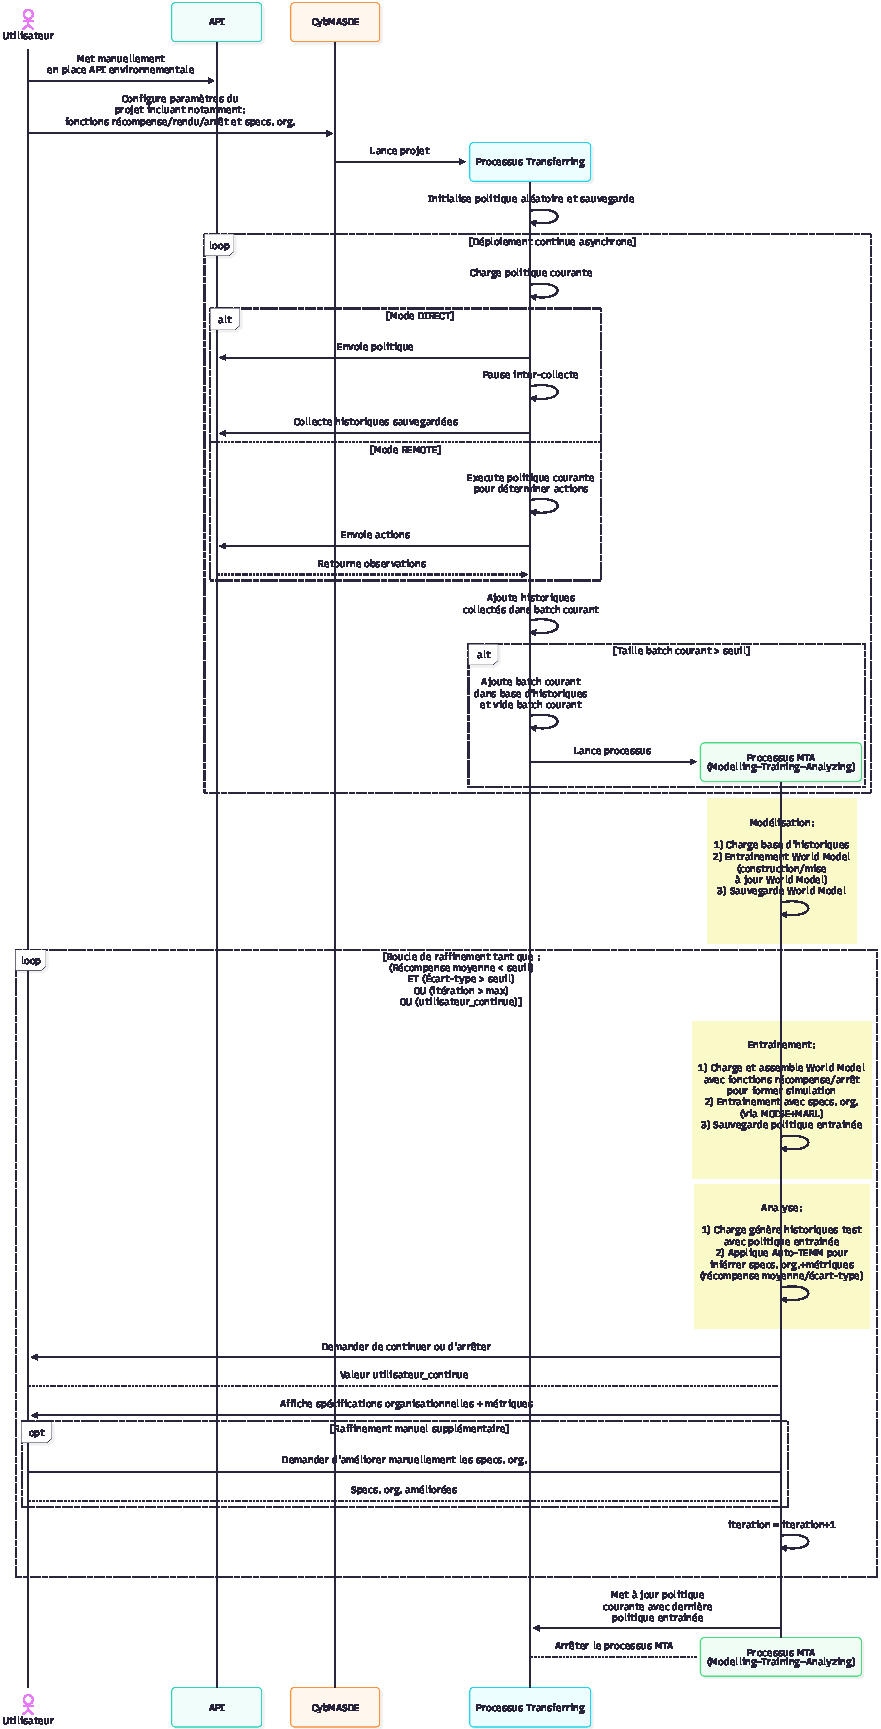
\includegraphics[trim={0cm 0cm 0cm 0cm},clip,height=\textheight]{figures/diagramme_sequence_CybMASDE.pdf}
% }
\caption{Sequence diagram for using CybMASDE}
\label{fig:cybmasde_sequence}
\end {figure}

\paragraph{2. \textit{Transferring} process}

If the project configuration is correct, the entire pipeline is launched in automatic mode with the command $\texttt{cybmasde run --full-auto}$. This creates and executes the \textit{Transferring} process, which is a continuous process that runs independently of the others. For the first execution, this process initializes a random policy and saves it locally in the project folder, along with an empty batch of joint histories.

Then, the execution of \textit{Transferring} enters an asynchronously executed loop that allows the deployed policies and the simulation model to be updated. In this loop, \textit{Transferring} loads the latest trained policy and deploys it in the real environment using the environmental API in two possible modes:
\begin{itemize}
  \item in \textit{DIRECT} mode, the policy is sent directly to the agents who execute it locally, storing their own histories which are retrieved and concatenated in the current batch at regular intervals via the environmental API;
  \item in \textit{REMOTE} mode, the policy is executed on the \acn{CybMASDE} side, actions are sent via the environmental API, observations are received, and new histories are thus formed on the \acn{CybMASDE} side and stored in the current batch.
\end{itemize}

Still in this loop, if the current batch of stored joint histories exceeds a threshold in terms of the number of joint histories (defined in the configuration), then it is saved in the history database (which is a simple folder containing the joint histories in JSON format) and emptied. This backup automatically triggers the \textit{MTA} process.

\paragraph {3. MTA process: Modeling–Training–Analyzing}

The \textit{MTA} process is therefore triggered each time a batch of new joint histories is added in order to take into account changes in the environment and generate appropriate policies. This process is independent of \textit{Transferring} and sequentially executes the three main activities: \textit{Modeling}, \textit{Training}, and \textit{Analyzing}. Each step uses the data and configurations provided by the user to accomplish its specific task.

First, in the modeling activity, if a simulated environment \textit{PettingZoo} has already been provided in the configuration file settings, it is loaded. Otherwise, an environment is generated by training a \textbf{World Model} from the latest recorded data. In the latter case, the last saved \textbf{World Model} is loaded (if it does not yet exist, then a new \textbf{World Model} is created). Next, all joint histories saved in the database are loaded to train the \textbf{World Model} using the hyperparameters provided in the configuration file. Once training (or updating) is complete, the \textbf {World Model} is then saved locally. A simulated \textit{PettingZoo} environment is then created from the trained \textbf{World Model} and the information manually provided by the user in the configuration: the initial joint observations, the action/observation space, the reward, rendering (optional), and stopping functions.

\noindent \textbf{Refinement loop} \\

Next, the \textit{MTA} process enters a refinement loop that only stops when the learned joint policy reaches a certain level of performance and stability, or when the maximum number of iterations is reached, or when the user decides to stop the process. In this loop, the joint policy is improved with each iteration by alternating between training and analysis activities.

In the training activity, the simulated environment set up previously is loaded to train the multi-agent policies using the MOISE+MARL implementation (see \autoref{sec:cybmasde_tech_stack}) to take into account the organizational specifications. Following the hyperparameters defined in the configuration, training is performed with a chosen algorithm (MAPPO, MADDPG, QMix, etc.) and according to a given maximum number of episodes. Once training is complete, the learned joint policy is saved locally in the project folder. Once training is complete, the analysis activity is launched.

In the analysis activity, the learned joint policy is loaded and evaluated by running several episodes in the simulated environment (according to the value of the sliding window on the last episodes). The resulting trajectories are collected and analyzed using the \acn{Auto-TEMM} or \acn{TEMM} method depending on the parameters given in the configuration file. Implicit organizational specifications (roles, objectives) are obtained in the form of constraint guides (mainly RAG and GRG) as well as organizational adequacy metrics (\acn{SOF}, \acn{FOF}, \acn{OF}). The stability of the policy is also evaluated by calculating the variance of the rewards obtained over these episodes as well as the average reward over these same episodes. The results of the analysis are saved locally in the project folder. At this point, the user is invited to consult the results of the analysis to decide whether to continue, stop, or manually refine the organizational specifications (for example, keep the most relevant observation-action rules). To do this, they can use a series of figures (visualizations \acn {PCA} visualizations and dendrograms of trajectories including centroids calculated by \acn{Auto-TEMM}/\acn{TEMM}).

\

The refinement loop continues until the average reward reaches the set threshold, the standard deviation remains above the stability threshold, the maximum number of iterations is reached, or the user chooses to continue. When the refinement cycles are complete, as with all trained policies, the last joint policy learned is also saved to be loaded by the \textit{Transferring} process, which continues its parallel execution. The \textit{MTA} process then stops until the next time a new batch of joint histories is added to the joint history database.


\medskip
In summary, \acn{CybMASDE} articulates two parallel processes: \textit{Transferring}, responsible for continuous deployment and data collection, and the \textit{MTA} process, triggered periodically to model, train, analyze, and refine policies.
User interactions occur mainly during initial configuration, refinement loop control, and final deployment.

\section{Life cycle implemented on Overcooked-AI}

\autoref{fig:cybmasde_cycle} shows the usage cycle of \acn{CybMASDE}.
To make this process more concrete, we provide a detailed step-by-step tutorial using the example of the \textbf{Overcooked-AI}~\cite{overcookedai} environment, which simulates a cooperative kitchen where two agents must prepare and serve soups. \autoref {tab:cybmasde_config} describes the configuration of this project.


\subsection{Initial configuration between the user, the real environment, and CybMASDE}

The user begins by installing Overcooked-AI and running a local instance accessible via a REST API, in order to \textquote{simulate a real environment} (and allow \acn{CybMASDE} to interact directly with the environment via the environmental API, which happens to be a REST API in another process -- see \autoref{appendix:cybmasde-environment-api}) . This setup step consists of preparing a daemon that manages the agents, the state of the kitchen, and the rules of the game. On the \acn{CybMASDE} side, no processes are activated yet: the platform simply waits for a project to be created and its configuration to be initialized before it can start the complete cycle.

\noindent
\textbf{Creating a project} \quad
Once the environment is ready, the user creates a new project with the command $\texttt{cybmasde init -n overcooked\_coop --template worldmodel}$. This command automatically generates the working tree, with the folders $\texttt{modeling}$, $\texttt{training}$, $\texttt{analyzing}$, and $\texttt{transferring}$. A central file $\texttt{project\_configuration.json}$ is also produced, serving as an entry point for the project description. At the same time, \acn{CybMASDE} creates template files such as $\texttt{label\_manager.py}$ and reward or stop function skeletons to guide the user in completing the essential elements.

\noindent
\textbf{Providing the initial elements} \quad
In this phase, the user fills in the $\texttt{project\_configuration.json}$ file. They describe the spaces for actions and observations needed to represent the kitchen environment: agent movements, picking up and putting down ingredients, cooking and serving actions. They then define a $\texttt{reward()}$ function that awards a point when soup is served, for example, and possibly a penalty in the event of a collision between the two agents. A termination criterion is set, such as a limit of 30 game steps. The user can leave the $\texttt{handcrafted\_environment.py}$ file empty, in which case no \acn{MCAS} model is used. Once these elements have been entered, the user executes the $\texttt{cybmasde validate}$ command, which allows \acn{CybMASDE} to check the consistency and completeness of the configuration. If there is an error, execution is interrupted with an explicit message; otherwise, the project is ready to be executed.

\subsection{Transferring process}
Once a satisfactory joint policy has been obtained, it is deployed in the real environment with the command $\texttt{cybmasde deploy --remote --api http://localhost:5000/api}$. In this mode, the policy is executed by \acn{CybMASDE}, which sends actions to the game agents and receives their observations. The $\texttt{--direct}$ mode, which directly integrates the policy into the agents, is also possible, but has not been considered here. Throughout the deployment and \textit{MTA} process, the \textit{Transferring} process continues to collect new traces that can be used to feed subsequent refinement cycles.

\begin{figure}[H]
  \centering
  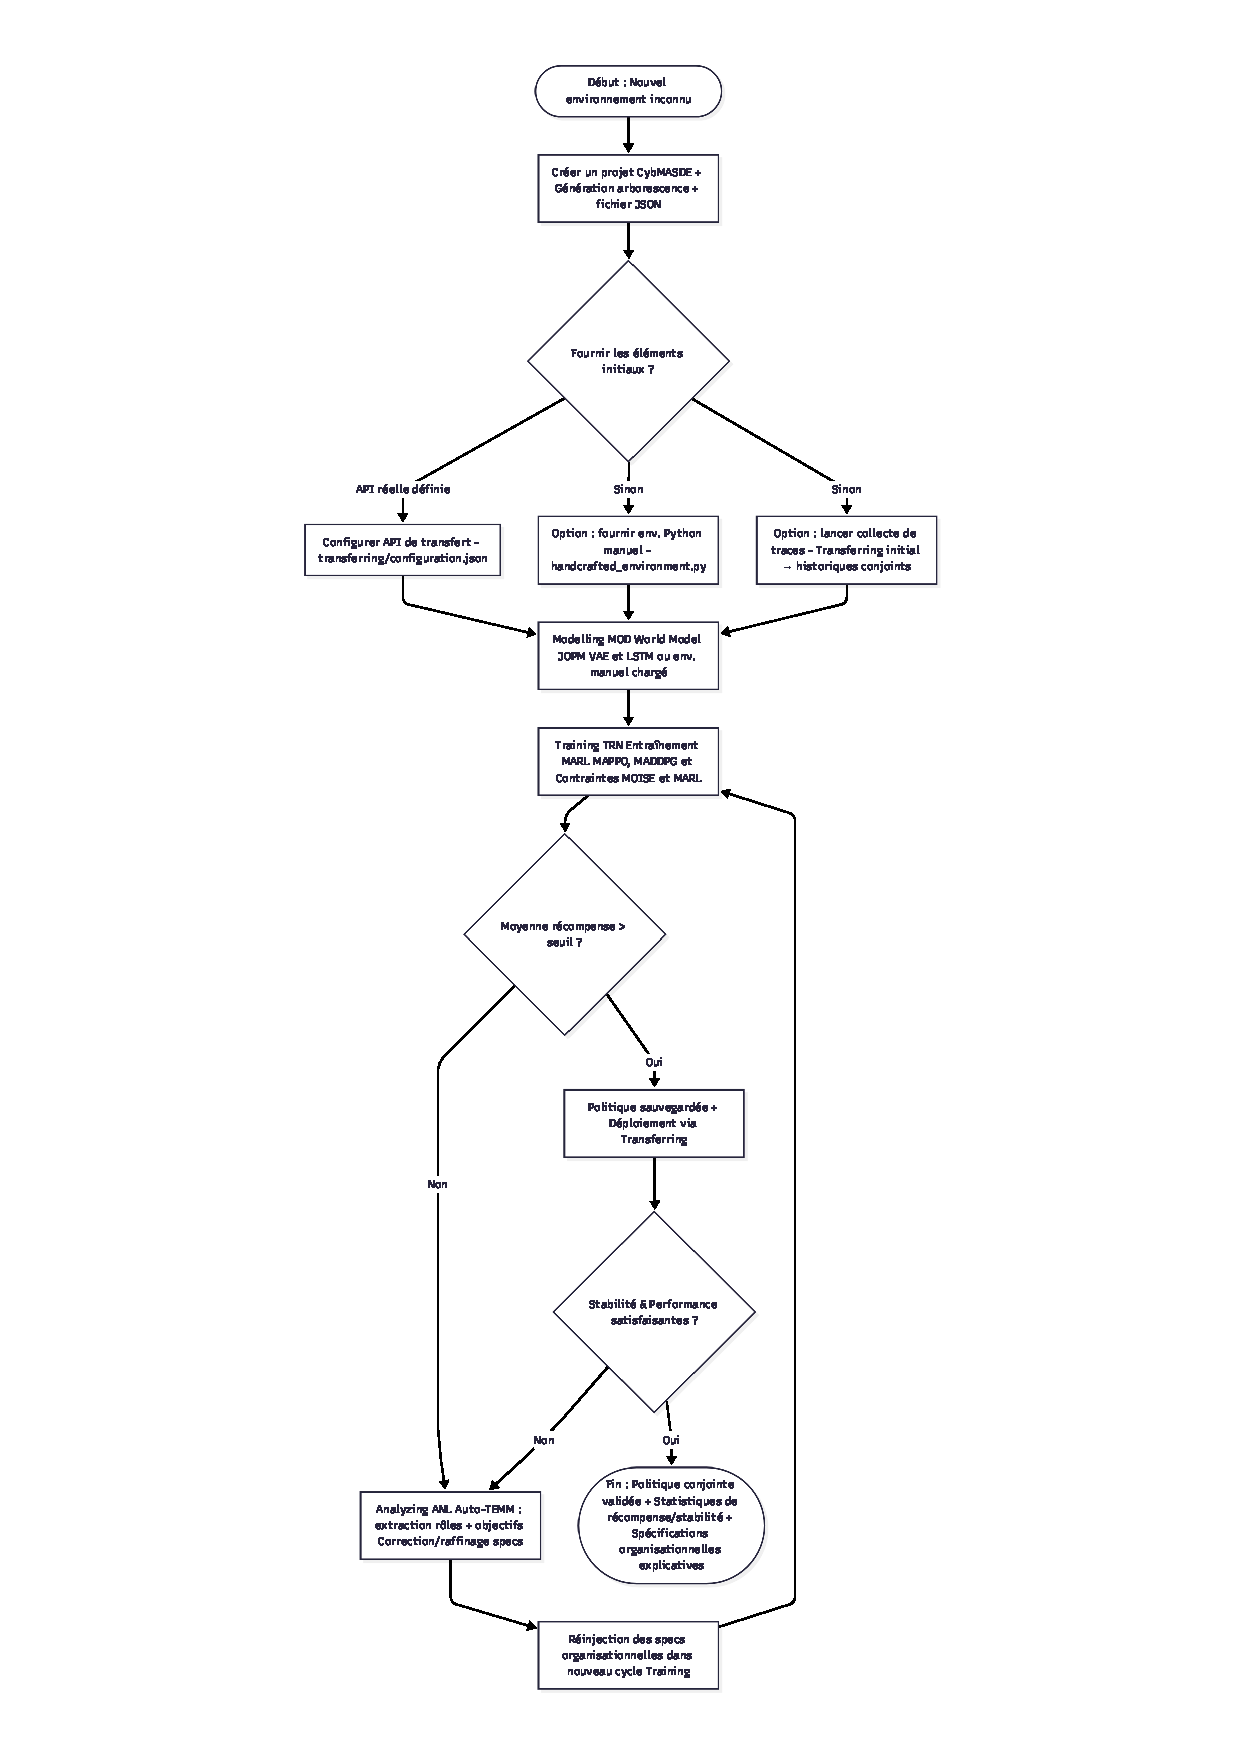
\includegraphics[trim={5cm 1cm 5cm 1cm},clip,height=\textheight]{figures/CybMASDE_user_flowchart.pdf}
  % }
  \caption{CybMASDE usage cycle}
  \label{fig:cybmasde_cycle}
\end{figure}

\subsection{MTA Process: Modeling–Training–Analyzing}

\noindent
\textbf{Modeling} \quad
The command $\texttt{cybmasde model --auto}$, \acn{CybMASDE} is launched and proceeds with an initial collection of trajectories by executing a random policy in Overcooked-AI. The two agents then move around aimlessly, sometimes picking up an onion or occupying the same squares in the kitchen. This raw data is used to train a \acn{JOPM} type \textbf{World Model}. This model consists of a variational encoder (VAE) that compresses the agents' joint observations into latent vectors and an RNN+MLP (\acn{RLDM}) network that predicts the next joint observation based on the action performed. The trained model is then saved in the $\texttt{generated\_environment/}$ folder and forms the basis of a simulated environment equivalent to that of Overcooked-AI, which can be used without requiring the actual API.

\

\noindent
\textbf{Training} \quad
Once the simulated model of the environment has been generated, the agents are trained automatically with the command $\texttt{cybmasde train --algo MAPPO}$. \acn{CybMASDE} then mobilizes $\texttt{MARLlib}$ and $\texttt{Ray RLlib}$ to perform multi-agent learning. The organizational roles defined by MOISE+MARL guide the process: one agent specializes in picking and preparing onions (cook), the other in serving soup (server), and versatile roles are also considered (see \autoref{lst:org_spec_oa}). As training progresses, checkpoints are saved along with reward curves that allow performance to be tracked over episodes.

\begin{lstlisting}[language=Python,basicstyle=\scriptsize, label={lst:org_spec_oa}, caption={Excerpt from the organizational configuration file for Overcooked-AI}]
organizational_model(
structural_specifications(
roles={
"role_server": role_logic(label_manager=oa_label_mngr).register_script_rule(primary_fun),
"role_polyvalent": role_logic(label_manager=oa_label_mngr).register_script_rule(secondary_fun)},
role_inheritance_relations={}, root_groups={}),
functional_specifications=functional_specifications(
goals={}, social_scheme={}, mission_preferences=[]),
deontic_specifications=deontic_specifications(permissions=[], obligations=[
deontic_specification(
"role_server", ["agent_0"], [], time_constraint_type.ANY),
deontic_specification(
"role_polyvalent", ["agent_1"], [], time_constraint_type.ANY)
]))
\end{lstlisting}

\

\textbf{Analysis} \quad
In the configuration step, the user set a performance threshold, for example an average reward of 3.5 per episode. After training, the \acn{CybMASDE} analysis activity calculates the average rewards obtained by the agents and compares it to this threshold. In the case of Overcooked-AI, it is not uncommon for agents to achieve a lower average after the first few iterations.

The command $\texttt{cybmasde analyze --auto-temm}$ applies the \acn{Auto-TEMM} method to the collected trajectories (see \autoref{lst:cybmasde_auto_temm_output}). This analysis consists of grouping trajectories into clusters according to their similarity, inferring the implicit roles played by the agents, and calculating metrics of stability and organizational adequacy. In the Overcooked-AI environment, for example, we can observe that agent 0 systematically adopts a server behavior while agent 1 assumes a versatile one. The results of this analysis are saved in the $\texttt{analyzing/ }$ folder and can be viewed by the user (see \autocite{lst:cybmasde_auto_temm_spec_output}).


\begin{lstlisting}[language={},basicstyle=\scriptsize, label={lst:cybmasde_auto_temm_output}, caption={Excerpt from the log output after training and application of TEMM}]
Running TEMM analysis...
1. Loading trajectories...
2. Clustering trajectories...
3. Generating visualizations...
4. Computing centroids.. .
5. Selecting near-centroid trajectories...
6. Extracting roles and goals...
7. Summarizing roles and goals...
8. Computing organizational fit scores...
Structural Fit (SOF): 1.000
Functional Fit (FOF): 1.000
Overall Organizational Fit (OF): 1.000
Finished TEMM analysis
\end{lstlisting}


\begin{lstlisting}[language=json,basicstyle=\tiny, label={lst:cybmasde_auto_temm_spec_output}, caption={Extract of organizational specifications after inference to be analyzed for manual refinement}]
{
"role_2": {
"rules": [
{
"observation": [
0.6,
0.4,
0.0,
0.0,
...],
"action": 3,
"weight": 0.15
},
{
'observation': [...],
"action": [
0.0,
0.0,
-0.2,
-0.2,
...],
"weight": 0.15
},
{
"observation": [...],
"action": 5,
"weight": 0.15
}
],
"support": 8
},
"role_1": {
'rules': [
{
"observation": [
0.6,
0.4,
0.0,
0.0,
...],
"action": 0,
"weight": 0.19
},
],
"support": 8
},
"1": {
"rules": [
{
"observation": [
0.6,
0.4,
0.0,
0.0,
...],
'action': 2,
"weight": 0.15
},
],
"support": 8
}
}
\end{lstlisting}

\

\noindent
\textbf{Refinement loop}
If performance remains insufficient, the user can decide to restart a series of cycles with the command $\texttt{cybmasde refine --max 5 --interactive}$. In this mode, the system automatically alternates between \textbf{training} and \textbf{analysis}, re-injecting the manually corrected organizational specifications at each iteration or keeping those inferred by \acn{TEMM}/\ acn{Auto-TEMM}. In Overcooked-AI, this may mean strengthening the role of cook for one of the agents, or specifying several versatile roles to diversify strategies. The cycle repeats until the set threshold is reached or the maximum number of iterations is exceeded.

\

To conclude on this example based on the Overcooked-AI environment, \acn{CybMASDE} shows how, with just a few commands, it is possible to move from an unknown environment such as Overcooked-AI to an \acn{SMA} by reducing manual interventions.




\section{Technology base (development)}\label {sec:cybmasde_tech_stack}

The development of \acn{CybMASDE} is based on a set of technologies chosen to meet the constraints of performance, modularity, and accessibility.
Below, we describe the role of each of these technologies, the reasons for their selection, and their practical use in the pipeline.

\paragraph{Python (backend).}
The core of \acn{CybMASDE} is written in \textbf{Python}, which offers a rich ecosystem of machine learning and scientific orchestration libraries. Python was chosen because:
\begin{itemize}
  \item it allows for easy integration of existing multi-agent learning frameworks (MARLlib, Ray RLlib);
  \item it is suitable for rapid prototyping of complex models (e.g., World Models or custom reward functions);
  \item it is widely used in the research and industrial community, which promotes reproducibility.
\end{itemize}
All modules of the MTA+T pipeline (Modeling, Training, Analyzing, Transferring) are implemented in Python.

\paragraph{PyTorch.}
The choice of \textbf{PyTorch} meets two needs:
\begin{enumerate}
  \item training simulation models (autoencoders, LSTM, VAE) to build \textit{World Models};
  \item serve as a common backend for multi-agent reinforcement algorithms.
\end{enumerate}
Its flexible API allows the implementation of specific network architectures, and its integration with CUDA ensures accelerated training on GPUs.

\paragraph{MARLlib and Ray RLlib.}
For multi-agent training, \acn{CybMASDE} uses \textbf{MARLlib} backed by \textbf{Ray RLlib}.
\begin{itemize}
  \item \textbf{MARLlib} provides a representative collection of reference algorithms (MAPPO, MADDPG, QMix, COMA, etc.) already configured for multi-agent.
  \item \textbf{Ray RLlib} ensures scalability: it allows distributed training to be executed on multiple GPUs or HPC nodes, which is essential for our cyberdefense experiments.
\end{itemize}
This combination was chosen to avoid reimplementing each algorithm while ensuring good performance on clusters.

\paragraph{Optuna.}
Hyperparameter optimization is delegated to \textbf{Optuna}, a flexible library that:
\begin{itemize}
  \item automatically explores the hyperparameter space (learning rate, discount factor, network size, clipping coefficients, etc.);
  \item integrates early stopping strategies (pruning) to save computation time;
  \item allows exploration ranges to be set in the project configuration file.
\end{itemize}
The use of Optuna ensures that each experiment makes efficient use of the available computing resources.

\paragraph{Angular (frontend).}
Although the main use of \acn{CybMASDE} remains the command line, an \textbf{Angular graphical interface} is also available.
Its purpose is to:
\begin{itemize}
  \item provide a unified view of the project configuration (rather than directly modifying the file tree);
  \item facilitate the monitoring of activities through dedicated tabs (modeling, training, analysis, transfer);
  \item allow the injection and visualization of execution traces or metrics without coding.
\end{itemize}
Angular was chosen because it allows for the rapid development of a modular, modern, and easily extensible web interface.

\paragraph{REST API and CLI.}
The pivot between these components is an internal \textbf{REST API}:
\begin{itemize}
  \item all CLI commands ($\texttt{cybmasde init}$, $\texttt{cybmasde train}$, etc.) call this API;
  \item the Angular interface also communicates via this API, which ensures consistency between the graphical mode and the console mode.
\end{itemize}
Thus, the CLI and frontend simply expose two different modes of access to the same backend.

\medskip
\noindent
In summary, the technological base combines \textbf{Python/PyTorch} for computation, \textbf{MARLlib + RLlib} for multi-agent learning, \textbf{Optuna} for optimization, and \textbf{Angular + REST + CLI} for accessibility.

\paragraph{Software architecture and classic interactions}

The C4 component deployment diagram (see \autoref{fig:cybmasde_uml}) illustrates the \acn{CybMASDE} modules and their sequence during typical use.

\begin{enumerate}
  \item The \textbf{user} interacts either via the \textbf{CLI} or via the \textbf{Angular} interface.
  \item These two access points call the same \textbf{REST API} from the backend.
  \item The REST API triggers the \textbf{Transferring process}, which:
        \begin{itemize}
          \item communicates with the \textbf{environmental API} of the target environment (real or simulated);
          \item continuously generates and stores histories in the local project database.
        \end{itemize}
  \item As soon as a batch of histories is complete, the \textbf{MTA} process is activated: it successively instantiates the \textbf{Modeling}, \textbf {Training}, and \textbf{Analyzing} modules.
  \item The results (trained policies, metrics, organizational specifications) are stored and made available to the user (via \acn{CLI} or interface).
\end{enumerate}

\begin{figure}[H]
\centering
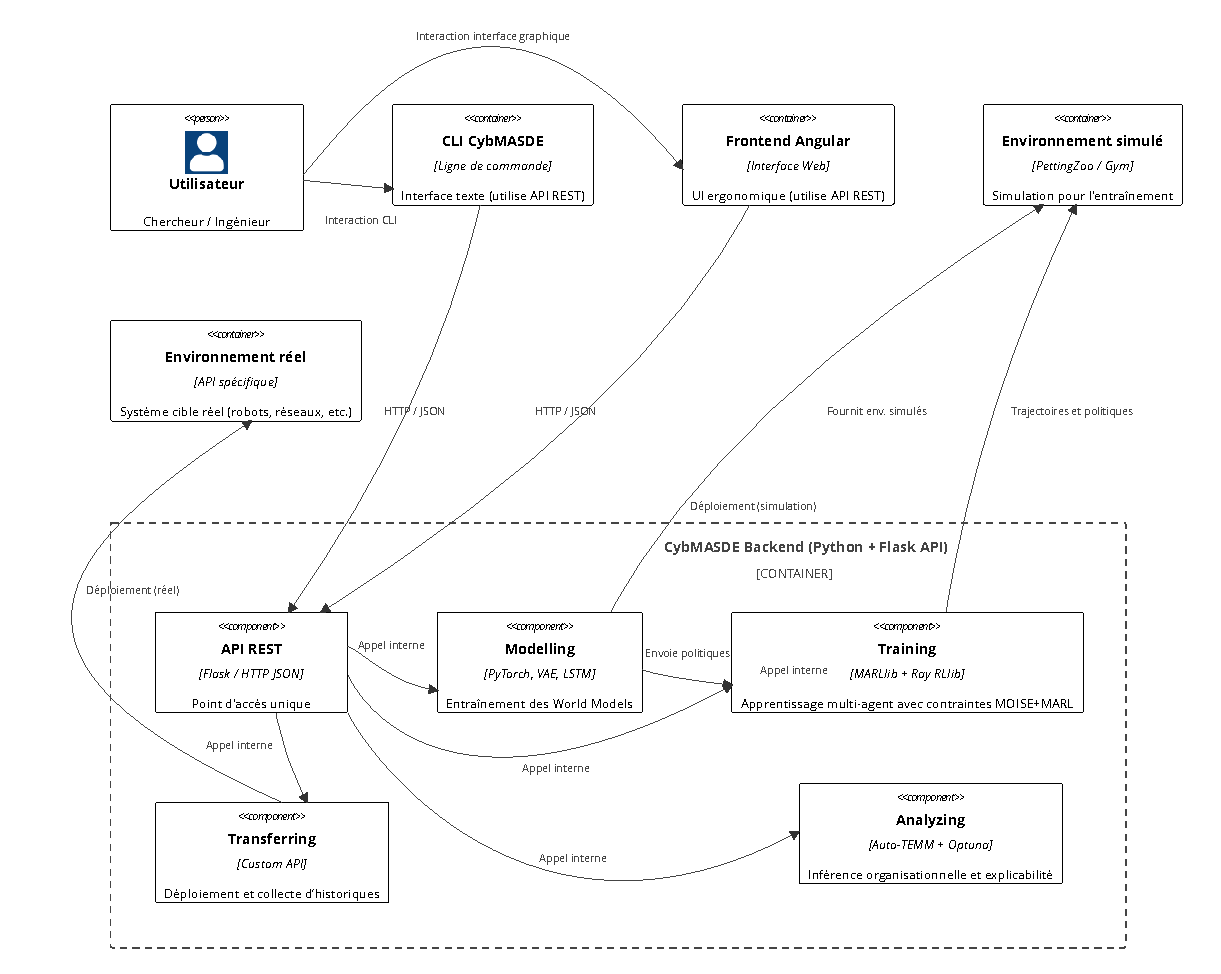
\includegraphics[width=\textwidth]{figures/CybMASDE_internal_component_diagram.pdf}
\caption{C4 component diagram illustrating the software architecture of CybMASDE}
\label{fig:cybmasde_uml}
\end {figure}

\section{Integration of the different contributions}

\subsection{Implementation of the pre-specialized Dec-POMDP model for Cyberdefense}

In addition to automatic modeling based on \textit{World Models}, we propose a manual modeling approach guided by a pre-specialized model for Cyberdefense environments.
The development of the \acn{Dec-POMDP} formalism applied to this domain has led to a model that we call \acn{MCAS} (\textit{Multi-Cyberdefense Agent Simulator}). This is a specific instance of \acn{Dec-POMDP} adapted to the explicit description of Cyberdefense scenarios.

\paragraph {Why an MCAS model?}
In cyberdefense environments, it is sometimes difficult to collect enough historical data to feed a \textit{World Model}. In addition, some defensive behaviors are better specified by experts. MCAS therefore allows:
\begin{itemize}
  \item to give the user a "turnkey" entry point for modeling a specific environment;
  \item structure the description in accordance with the Dec-POMDP formalism (observations, actions, transitions, rewards, termination);
  \item directly integrate this model into the CybMASDE cycle.
\end{itemize}

\paragraph{How is it provided?}
When a project is created, CybMASDE generates a template file in \textquote{modeling/simulated\_environment/handcrafted\_environment.py}.

This file is a Python interface with gaps that the user must fill in by defining:
\begin{itemize}
  \item the observation space (e.g., status of a server or network node),
  \item the action space (e.g., block traffic, scan a port, restart a service),
  \item the transition dynamics (how the environment evolves after an action),
  \item the reward function (bonus/penalty depending on successful defense or attack),
  \item the stopping function (episode end conditions).
\end{itemize}

\paragraph{Execution and integration.}
Once completed, MCAS is automatically recognized by CybMASDE:
\begin{itemize}
  \item it can be run in simulation mode to generate multi-agent training trajectories;
  \item it is compatible with "turn-based" mode: the user can view the evolution of the environment in real time, represent the topology in graph form, and consult metrics (cumulative rewards, success rates, etc.);
  \item it can also be serialized in JSON format in order to share or reuse the description of the environment.
\end{itemize}

Thus, MCAS offers a manual and structured alternative to automatic modeling, ensuring that simulation environments remain appropriate and understandable in cyberdefense scenarios while integrating naturally into the \acn{MTA}+T chain of \acn{CybMASDE}.


\subsection{Implementation of the MOISE+MARL framework}

One of the key contributions of \acn{CybMASDE}\footnotemark[1] is to integrate the MOISE+ organizational framework with multi-agent learning methods. To do this, we have developed a Python implementation called \acn {MMA}\footnotemark[2].

\footnotetext[2]{ \label{fn:github} The \textquote{MOISE+MARL API} implementation (\acn{MMA}), the hyperparameters and specifications used are available at \url {https://github.com/julien6/MOISE-MARL}. A demonstration video is also available at \url{https://www.youtube.com/watch?v=b3wqFpfXZi0}.}


\paragraph{Why MMA?}
The MOISE+ framework allows organizations (roles, missions, permissions) to be formalized, but its direct use can be tedious. \acn{MMA} aims to:
\begin{itemize}
  \item encapsulate MOISE+ relationships in the form of object-oriented Python classes,
  \item minimize manual intervention by offering a clear, ready-to-use API,
  \item easily interface with simulated environments (\acn{Dec-POMDP}, PettingZoo).
\end{itemize}

\paragraph{Internal structure.}
The \acn{MMA} API defines:
\begin{itemize}
  \item a root class $\texttt{Moise}$, containing roles, objectives, and permissions;
  \item specialized classes for each type of constraint guide (e.g., $rag$, $rrg$, $grg$);
  \item a dictionary for mapping action/observation labels to organizational behaviors.
\end{itemize}
These guides can be instantiated either by Python code or by JSON rules.

\paragraph{Integration with PettingZoo.}
To interact with a multi-agent environment, \acn{MMA} encapsulates it in a PettingZoo \textit{wrapper}:
\begin{itemize}
\item action masks are automatically applied to prevent agents from violating organizational constraints,
\item rewards are adjusted according to organizational objectives (shaping),
\item consistency between prescribed organization and emerging behaviors is ensured during training.
\end {itemize}

\paragraph{Link to training.}
\acn{MMA} integrates naturally with \textbf{MARLlib} and \textbf{Ray RLlib}:
\begin{itemize}
  \item the user chooses an algorithm (MAPPO, QMix, MADDPG, etc.);
  \item the \acn{MMA} wrapper applies MOISE+ constraints on top of the chosen algorithm;
  \item the training results therefore take into account not only performance, but also compliance with organizational specifications.
\end{itemize}

\paragraph{Post-training analysis.}
After training, CybMASDE applies the \acn{TEMM} (or \acn{Auto-TEMM}) method to:
\begin{itemize}
  \item automatically identify implicit roles and missions,
  \item represent behaviors using hierarchical clustering and K-means,
  \item generate visual outputs (role dendrograms, transition graphs),
  \item export the inferred specifications in JSON format for reuse.
\end{itemize}

\

In summary, \acn{MCAS} offers specialized manual modeling for cyber defense, while \acn{MMA} provides an operational organizational framework integrated into the learning cycle. Their combination in \acn{CybMASDE} makes it possible to combine organizational rigor with multi-agent training flexibility.


\section{Conclusion}

This chapter presented the implementation of \acn{MAMAD} through the \acn{CybMASDE} platform. The modular approach, structured around modeling, training, analysis, and transfer, has been adapted to various scenarios, from toy environments to real-world cases in cyber defense and microservices.
The integration of MOISE+MARL into the multi-agent learning pipeline has made it possible to obtain policies that are consistent with organizational objectives. \acn{CybMASDE} is available as open-source software\footnotemark [1].

Despite these contributions, limitations remain: dependence on trace quality, high computational requirements, difficulty in generalizing to constrained distributed systems, and explainability that could still be improved. This chapter thus lays the foundations for advanced automation of organizational design in \acn{MARL}, paving the way for future optimizations and applications on real \acplu{SMA}.

\footnotetext[1] { \label{fn:github} The \textquote{CybMASDE} implementation not only brings together our contributions, but also integrates a significant number of packages, resulting in a relatively large software package ($\sim$250,000 lines of code) once the dependencies are installed: \url{https://github.com/julien6/CybMASDE}.}

\clearpage
\thispagestyle{empty}
\null
\newpage


\chapter{Experimental and evaluation framework}
\label{chap:experimental_framework}

The purpose of this chapter is to define a generic experimental framework applicable to all case studies presented in \autoref{chap:case_studies}. The objective is to provide a \textit{framework} that each scenario can instantiate by specifying the chosen elements of the \acn{MAMAD} method. This framework is based on the \acn{MAMAD} method, the taxonomy of activities and sub-activities presented in \autoref{tab:mamad_taxonomy}, and the evaluation criteria defined above.

\section{Description of the sets of environments and algorithms considered}

To ensure the generality and robustness of the evaluation, we consider a varied set of reference environments from the \acn{MARL} literature:
\begin{itemize}
\item \textbf{Overcooked-AI}~\cite{overcookedai}: a complex cooperative toy-type environment requiring coordination and sequential planning.
\item \textbf{Predator-Prey}~\cite{lowe2017multi}: a chase-and-escape toy-type environment used to test coordination and competition.
\item \textbf{Warehouse Management}: a new toy environment that we proposed to simulate multi-agent logistics management with flow and resource constraints.
\item \textbf{Company Infrastructure}~\cite{cyberbattlesim}: a simulation of attacks and defenses on a network, inspired by MITRE ATT\&CK.
\item \textbf{Drone Swarm}~\cite{cage_challenge_3_announcement}: a simulation of a swarm of drones subjected to software attacks and requiring collective defense.
\item \textbf{Kubernetes Microservices}: a real environment consisting of a cluster of four interconnected microservices that we proposed for the orchestration of microservices with auto-scaling and resilience against intentional failures.
\end {itemize}

The \textbf{Kubernetes Microservices} environment differs from the others in that it is real: it is a system of four interconnected services, whereas the other environments are simulated. For practical reasons, the simulated environment serves as a "real" reference, allowing \acn{MAMAD} to be applied as if on an operational system, with the \textit {World Model} acting here as a simulation of the simulation. This choice validates the principle of \acn{MAMAD}: if the \textit{World Model} reconstructed from traces is sufficiently accurate, the learned policies can be transferred effectively, thus facilitating comparison between simulation and reality. In this scenario, the \textbf{Kubernetes Microservices} environment can be used directly with \acn{MAMAD} without requiring additional modeling, and the transfer (\textbf{TRF}) is performed to this real system, demonstrating the validity of the approach in an operational context.

\medskip

The selected \acn{MARL} algorithms cover the main families recognized in the literature:
\begin{itemize}
  \item \acn{MAPPO}~\cite{Yu2022}\index{MAPPO}~: algorithm based on \acn{PPO}~\cite{Schulman2017} adapted to multi-agent systems, using centralized policies to stabilize learning while allowing decentralized execution.
  \item \acn{MADDPG}~\cite{lowe2017multi}\index{MADDPG}~: deterministic gradient learning method, combining individual policies with centralized criticism to handle multi-agent non-stationarity.
  \item \acn{QMIX}~\cite{rashid2018qmix}\index{QMIX}~: value factorization algorithm, combining individual Q-values of agents via a nonlinear mixing network to optimize a global reward.
  \item \acn{COMA}~\cite{foerster2018counterfactual}\index{COMA}~: actor-critic-based approach, using counterfactual estimation to accurately attribute each agent's contribution to the collective reward.
  \item \acn{IQL}~\cite{Jiang2022}\index{IQL}~: each agent learns its own Q function independently, without explicit coordination, which can lead to non-stationarity, but remains simple to implement.
  \item \acn{VDN}~\cite{sunehag2018value}\index {VDN}~: decomposes the overall value into a sum of the individual values of the agents, facilitating cooperative learning while maintaining a simple structure.
\end{itemize}
The environments are implemented via \textit{PettingZoo}~\cite{terry2020pettingzoo} and the algorithms via \textit{MARLlib}~\cite {hu2022marllib}.

\section{Reproducibility conditions}

\subsection{Experimental hardware conditions}
\label{par:compute_conditions}
The experiments are performed on an academic HPC cluster. Unless otherwise stated, the following constants apply to all scenarios:
\begin{itemize}
  \item Accelerators: NVIDIA A100 / V100, AMD MI210.
  \item \textbf{DL frameworks}: PyTorch~\cite{Paszke2019} and TensorFlow~\cite{Abadi2016} (implementations \acn{MARLlib}/\acn{MAPPO}, etc.)\index{PyTorch}.
  \item \textbf{Hyperparameter optimization}~: \textbf{Optuna}~\cite{akiba2019optuna} (\acn{TPE}) for \acn{LR}, exploration/exploitation, network sizes; standardized search space by algorithm family.
  \item \textbf{Parallelism}~: $\sim$ 5 independent executions per condition (algorithm $\times$ environment $\times$ constraint).
  \item \textbf{\acn{OS} and libs}~: Linux 64-bit, \acn{CUDA}/cuDNN or ROCm depending on \acn{GPU}; fixed environments (conda/pip).
\end{itemize}
The case studies only mention specific deviations (e.g., number of runs, particular GPU).

\subsection{Hyperparameter management (default and overrides)}
Each \{algorithm, environment\} pair is initialized with a standard profile from MARLlib and preliminary experiments.
A controlled \acn{HPO} pass can be performed with \textbf{Optuna} (bounded budget, same search space priorities between scenarios)~\cite{akiba2019optuna}. The best \textit{trial} is then \textbf{replayed 5 times} to aggregate the results.
Scenarios can:
\begin{enumerate}[label=\alph*)]
  \item accept default values,
  \item restrict \acn{HPO},
  \item explicitly override certain hyperparameters.
\end{enumerate}

\section{Experimental baselines}

An experimental baseline is a set of data used to reproduce the experiment. In our case, a baseline includes the following elements~:
\begin{itemize}
  \item \textbf{Activities}: A selection of \acn{MAMAD} activities.
  \item \textbf {Algorithm}: A \acn{MARL} algorithm or another algorithm from the literature that may enable agents to achieve their objectives using a different approach.
  \item \textbf{Organizational specifications}: A set of MOISE+MARL-type organizational specifications if the chosen algorithm belongs to the \acn{MARL} domain.
  \item \textbf{Environment}: An environment with scenario variants (e.g., Overcooked-AI~\cite{overcookedai}, Predator-Prey~\cite{lowe2017multi}, Drone Swarm~\cite{cage_challenge_3_announcement}).
  \item \textbf{Specific metrics}: A set of metrics specific to the environment or study (environment-specific).
  \item \textbf{Execution conditions}: A set of execution conditions (number of runs, seeds, hardware, possible disturbances).
\end{itemize}

In the context of experiments, certain characteristics of baselines (such as the environment or specific metrics) remain fixed. To instantiate a baseline, we therefore focus on variable elements such as the algorithm used, execution conditions, or organizational specifications. The main objective of defining baselines is to have points of comparison to measure the impact of the different components of the \acn{MAMAD} method method. By comparing the results obtained with these baselines, we can isolate and analyze the contribution of each activity (modeling, training, analysis, transfer) as well as the effect of organizational specifications on the behavior and performance of the \acn{SMA}.



\section{Evaluation grid}\label{sec:evaluation_grid}

\subsection{Criteria and associated metrics}\label{sec:criteria_metrics}

The evaluation is based on a grid of criteria (see \autoref{tab:grille}) inspired by the recommendations of the \acn{RL}/\acn{MARL} community~\cite{papoudakis2021agent}:

\begin{table}[h!]
  \centering
  \caption{Correspondence between overall criteria and metrics}
  \renewcommand{\arraystretch}{1.2}
  \begin{tabular}{ll}
    \hline
    \textbf{Criterion}   & \textbf{Associated metrics}                                    \\
    \hline
    C1 -- Autonomy       & Proportion of intervention (design/operation)                  \\
    C2 -- Performance    & Cumulative reward; Convergence rate                            \\
    C3 -- Adaptation     & Standard deviation of rewards; Robustness score                \\
    C4 -- Control        & Constraint violation rate; Consistency score                   \\
    C5 -- Explainability & Organizational suitability; Quality of inferred specifications \\
    \hline
  \end{tabular}
  \label{tab:grid}
\end{table}

These different metrics aim to determine the extent to which the five overall criteria (C1--C5) are covered on a given baseline.
Each metric is described separately for clarity.

\paragraph{Proportion of intervention (design/operation).}\index{Proportion of intervention}
\textit{Unit: percentage (\%). Source: platform usage logs, user questionnaires, automation scripts, number of refinement cycles, manual estimates.}
It is calculated as the following ratio:
\[
  \hspace{2.5cm}\frac{\text{estimated time for automated design}}{\text{estimated time for manual design}}
\]
This proportion, which is less precise, aims to quantify at least approximately the impact of automation on the design process: what percentage of manual interventions is necessary to achieve performance similar to manually designed and implemented \acplu{SMA}. It can be estimated via software instrumentation by indicating that a large number of refinement cycles increases the proportion of intervention (i.e., the ratio of the number of cycles used to the number of empirical cycles of manual design). Considering the already modeled environment, this proportion is also obtained manually by estimating the time spent (in number of hours) during completely manual design, which in our method corresponds to the estimated time spent (in number of hours) in the refinement cycles alternating between training and analysis.

\paragraph{Cumulative reward.}\index{Cumulative reward}
\textit{Unit: numerical value without unit (often normalized). Source: \acn{MARLlib}/RLlib training logs, episode result files.}
This is the sum of the rewards obtained by all agents over an episode or a sliding window.
It is extracted automatically via analysis scripts.

\paragraph{Convergence rate.}\index{Convergence rate}
\textit{Unit: number of episodes (integer). Source: learning curves, training logs. }
This corresponds to the number of episodes required for the average reward to exceed a predefined threshold and remain stable.
The calculation is automated by detecting a plateau on the learning curve.

\paragraph{Standard deviation of rewards.}\index{Standard deviation of rewards}
\textit{Unit: same as reward (often without unit). Source: training logs, results of multiple runs.}
This metric corresponds to the statistical standard deviation of average rewards between several independent runs.
It is calculated automatically when the results are aggregated.

\paragraph{Robustness score.}\index{Robustness score}
\textit{Unit: ratio or percentage (\%). Source: tests under disturbances (failures, attacks), episode logs.}
It is defined as:
\[
  \hspace{3.5cm}\frac{\text{performance under disturbance}}{\text{nominal performance}}
\]
This score is obtained by comparing average performance in disturbed scenarios and reference scenarios.
Disturbances are generated either by different seeds in simulated environments or by explicit changes (topology, failures, attacks, etc.).

\paragraph{Constraint violation rate.}\index{Constraint violation rate}
\textit{Unit: percentage (\%). Source: execution logs, environment wrappers, post-hoc analysis.}
The formula is:
\[
  \hspace{3.5cm}\frac{\text{number of violations detected}}{\text{total number of steps per episode}}.
\]
This measure evaluates the ability of agents to comply with the rules imposed by their roles.
It varies with the strictness of the constraints: a zero rate is expected when the strictness is maximum, and a high rate when the constraints are zero.
Intermediate values must be analyzed in relation to the cumulative reward in order to identify any overly restrictive rules that would reduce overall performance.

\paragraph{Consistency score.}\index{Consistency score}
\textit{Unit: ratio (0–1) or percentage (\%). Source: trajectory clustering, \acn{TEMM}/\acn{Auto-TEMM} analysis.}
This score measures the similarity between observed behaviors and expected roles.
The idea is to compare the original organizational specifications with those inferred automatically.
The smaller the distance between the two sets of trajectories, the higher the consistency score, indicating that MOISE+MARL has taken the organizational specifications into account and that \acn{TEMM}/\ acn{Auto-TEMM}.

\paragraph{Organizational adequacy.}\index{Organizational adequacy}
\textit{Unit: ratio (0–1). Source: \acn{TEMM} analysis, role-mission correspondence matrices.}
As explained previously in \autoref{sec:TEMM_algorithm}, it is calculated as a weighted average of the structural (\acn{SOF}) and functional (\acn{FOF}) scores with $\alpha = 0.5$ by default:
\[
  \hspace{3.5cm}\text{OF} = \alpha \cdot \text{SOF} + (1-\alpha) \cdot \text{FOF}.
\]
This measure quantifies the extent to which the learned policies comply with the expected organizational structure.

\paragraph{Quality of inferred specifications.}\index{Quality of inferred specifications}
\textit{Unit: percentage (\%) or similarity score. Source: automatic comparison between inferred specifications (\acn{JSON}, \acn{TEMM}) and reference specifications} .
This metric measures the quality of inferred organizational specifications by comparing their similarity to reference specifications, using indicators such as the Jaccard index~\cite{Jaccard1908} (proportion of shared elements) or the Euclidean distance. Unlike the consistency score, it focuses solely on the fidelity of the extracted specifications, regardless of the learned policies. The calculation is based on a systematic comparison between the inferred specifications and the initial specifications, varying the scenarios to evaluate the generalization capacity. The objective is to find a compromise between fidelity to the initial specifications and generalization capacity, avoiding overfitting and limiting the complexity of the inferred rules or objectives, while maximizing similarity with the reference trajectories.

\section{Experimentation and evaluation protocol}\label{sec:experimental_protocol}

The proposed experimental protocol follows a progressive reasoning similar to the practices of the community~\cite{papoudakis2021agent}.
Steps 1 to 4 constitute the experimental protocol, while steps 5 and 6 concern the evaluation of the results:

\paragraph{1. Initial configuration}
Required configuration including the implementation of the \acn{API} \acn{REST} for communication with the environment and the various components required to model the environment and other data necessary to create a \acn{CybMASDE} project for a given baseline.

\paragraph{2. Implementation of the advanced baseline}
Definition of at least one \textbf {advanced baseline} considered as the \textbf{default baseline}:
\begin{table}[h!]
  \centering
  \caption{Generic characterization of the \textquote{advanced baseline}}
  \label{tab:baseline_generic}
  \renewcommand{\arraystretch}{1.4}
  \footnotesize
  \begin{tabularx}{\textwidth}{
      >{\raggedright\arraybackslash\hsize=0.3\hsize}X
      >{\raggedright\arraybackslash\hsize=0.7\hsize}X
    }
    \hline
    \textbf{Element}              & \textbf{Instantiated value}                                                                                                \\
    \hline
    Environment                   & Name of the environment and possible scenario variants (e.g., Overcooked-AI, classic layout).                              \\
    Activities \acn{MAMAD}        & \acn{MOD-AUT},\acn{TRN-CON},\acn{ANL-AUT},\acn{TRF-AUT}                                                                    \\
    Algorithm                     & Selected algorithm with its implementation (e.g., \acn{MAPPO} via \acn{MARLlib}).                                          \\
    Organizational specifications & MOISE+MARL set containing both roles and missions.                                                                         \\
    Specific metrics              & Additional indicators specific to the environment (e.g., dishes served, collision rate, infected drones, average latency). \\
    Execution conditions          & Number of runs, seeds, type of hardware (\acn{CPU}/\acn{GPU}), disruptions/stress tests.                                   \\
    \hline
  \end{tabularx}
\end{table}

\paragraph{3. Implementation of alternative baselines}
Possible definition of other baselines based on other parameters such as \acn{MARL} algorithms, organizational constraints, or modeling according to the specific issues of each scenario. Baseline

\paragraph{4. Definition of ablation studies}
Conducting at least one \textbf{ablation study}: each ablation consists of taking the \textbf{advanced baseline} and changing one or more parameters, in particular replacing one or more \acn{MAMAD} activities with less advanced variants (for example, \textquote{\acn{ANL-MAN}} using \acn{TEMM} rather than \acn{Auto-TEMM}, or \textquote{\acn{TRN-UNC}} without organizational constraints), but also removing organizational constraints, changing algorithms, etc. Each ablation must be justified according to the specific questions of each scenario.

\paragraph{5. Comparison and validation}
Systematic comparison of results on the evaluation grid (\autoref{tab:grille}) to measure the impact of each component on the target criteria. The analysis of the results must include visualizations (learning curves, heatmaps, dendrograms, etc.) and a critical discussion of the compromises observed (e.g., performance vs. compliance with constraints).

\paragraph{6. Repetition and aggregation}
Repetition of experiments (5 independent runs, recorded seeds), statistical aggregation (mean, standard deviation), and statistical tests (t-test or non-parametric depending on normality).


\section {Summary}

This chapter laid the methodological foundations for the experimental evaluation of the \acn{MAMAD} method. By defining a generic, reproducible, and structured framework, it allows for the comparison of performance, robustness, and explainability of the method in various environments, ranging from toy cases to real systems. The major advantage of this framework is that it ensures the traceability of choices, the transparency of protocols, and the validity of results, while facilitating critical analysis of the contributions and limitations of each component of the method. This methodological framework is essential for ensuring the scientific credibility of experiments and identifying levers for future improvement. The following chapters draw on this framework to instantiate, analyze, and discuss the application of \acn{MAMAD} in concrete contexts, highlighting its ability to meet the criteria of autonomy, performance, adaptability, control, and explainability.


\clearpage
\thispagestyle{empty}
\null
\newpage


\chapter{Case Studies}
\label{chap:case_studies}

This chapter presents case studies conducted to evaluate the \acn{MAMAD} method in various contexts. Each section details the instantiation of the experimental framework defined in \autoref {chap:experimental_framework} for a specific environment, specifying the methodological choices and experimental configurations.

\section{Experiments on non-Cyberdefense-oriented environments}

In this section, we describe the experiments that were conducted on a set of non-Cyberdefense-oriented reference environments. The main objective is to validate the \acn{MAMAD} method in various contexts, with an emphasis on coordination, competition, and resource management in partially observed environments. The goal is to provide proof of concept that the \acn{MAMAD} method is applicable to simple cases. From there, it is possible to effectively address its application to scenarios strictly related to cyberdefense.

This section proposes the same instance of the \autoref{sec:protocole_experimental} experimentation protocol (steps 1 to 4) for three non-cyber defense-oriented environments (\textit{Overcooked-AI}, \textit{Predator-Prey}, \textit{Warehouse Management}).
The objective is to describe the experiments to be conducted to apply the evaluation protocol of \autoref{sec:experimental_protocol} (steps 5 to 6) in the following chapter in order to validate the \acn{MAMAD} method in various cooperative/competitive contexts, with partial observation and coordination requirements.


\subsection{Description of environments}

\subsubsection*{Overcooked-AI}

The \textbf{Overcooked-AI}~\cite{Carroll2019} environment simulates a cooperative cooking scenario where agents must collaborate to prepare and serve meals in a structured kitchen. This environment is illustrated in \autoref{fig:overcooked}\index{Overcooked-AI}.

% \begin{enumerate*}[label={\roman*)}, itemjoin={; \quad}]
\begin{itemize}
  \item \textbf{State space:} A discrete grid-based kitchen with workstations (cutting board, stove, serving counter), ingredients, and agents
  \item \textbf{Observation space:} Agents observe kitchen elements within a defined radius
  \item \textbf{Action space:}
        \begin{enumerate*}[label={\roman*)}, itemjoin={; \quad}]
          \item Movement: \textquote{Up, Down, Left, Right}
          \item Interact: \textquote{Choose an ingredient, cut, cook, serve}.
        \end{enumerate*}
  \item \textbf{Reward structure:}
        \begin{enumerate*}[label={\roman*)}, itemjoin={; \quad}]
          \item Successful meal preparation: $+20$
          \item Incorrect use of ingredients: $-5$
          \item Passive behavior: $-1$ per step without significant action.
        \end{enumerate*}
  \item \textbf{Objective:} Maximize the number of meal orders completed within a set time limit.
\end{itemize}
% \end{enumerate*}
%
\textbf{Organizational specifications:}
% \begin{enumerate*}[label={\roman*)}, itemjoin={; \quad}]
\begin{itemize}
  \item \textbf{Roles:} \textquote{Chef, assistant, server}
  \item \textbf{Tasks:} The chef prepares the dishes, the assistant provides the ingredients, and the server serves the meals
  \item \textbf{Constraints:} Tasks must be synchronized to avoid bottlenecks.
\end{itemize}
% \end{enumerate*}

\begin{figure}[h!]
  \centering
  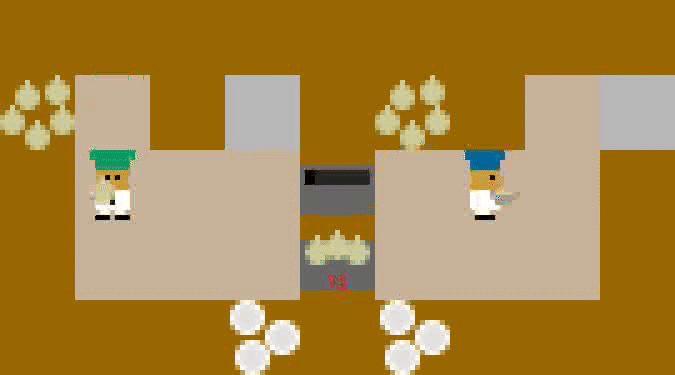
\includegraphics[trim=0cm -0.5cm 0cm -0.5cm, clip, width=0.9\linewidth]{figures/overcooked.png}
  \caption[Screenshot of the Overcooked-AI environment]{Screenshot of the Overcooked-AI environment: two agents (chefs) must collaborate to efficiently prepare and serve onion soups. The process involves taking three onions (one at a time) from the dispenser, placing them in a pot, waiting for the soup to cook, fetching a clean bowl, ladling the soup, and delivering it to the serving counter. The layout of the kitchen includes obstacles and narrow passages, requiring the agents to coordinate their movements to avoid collisions and optimize task completion.}
  \label{fig:overcooked}
\end{figure}

\subsubsection*{Predator-Prey}

The \textbf{Predator-Prey} environment is a well-known \acn{MARL} benchmark~\cite{lowe2017multi}, designed to evaluate coordination between cooperative pursuers (predators) attempting to capture an elusive agent (prey) . This environment is illustrated in \autoref{fig:predator_prey}\index{Predator-Prey}.
%
% \begin{enumerate*}[label={\roman*)}, itemjoin={; \quad}]
\begin{itemize}
  \item \textbf{State space:} A continuous 2D space where agents (predators and prey) have positions $(x, y)$ and velocities
  \item \textbf{Observation space:} Agents detect nearby entities within a limited radius $r$
  \item \textbf{Action space:}
        \begin{enumerate*}[label={\roman*)}, itemjoin={; \quad}]
          \item Movement: \textquote{Up, Down, Left, Right, Stay in place}.
        \end{enumerate*}
  \item \textbf{Reward structure:}
        \begin{enumerate*}[label={\roman*)}, itemjoin={; \quad}]
          \item Predators earn $+50$ for each prey captured
          \item Prey earns $+1$ per time step survived;.
        \end{enumerate*}
  \item \textbf{Objective:} Predators must cooperate to trap the prey, while the prey tries to escape for as long as possible.
        % \end{enumerate*}
\end{itemize}
%
\textbf{Organizational specifications:}
% \begin{enumerate*}[label={\roman*)}, itemjoin={; \quad}]
\begin{itemize}
  \item \textbf{Roles:} \textquote{Predator, Prey}
  \item \textbf{Missions:} Predators coordinate their efforts to surround the prey; the prey seeks the best escape routes
  \item \textbf{Constraints:} Predators must find a balance between aggressive pursuit and blocking strategies.
        % \end{enumerate*}
\end{itemize}
%
\begin{figure}[h!]
  \centering
  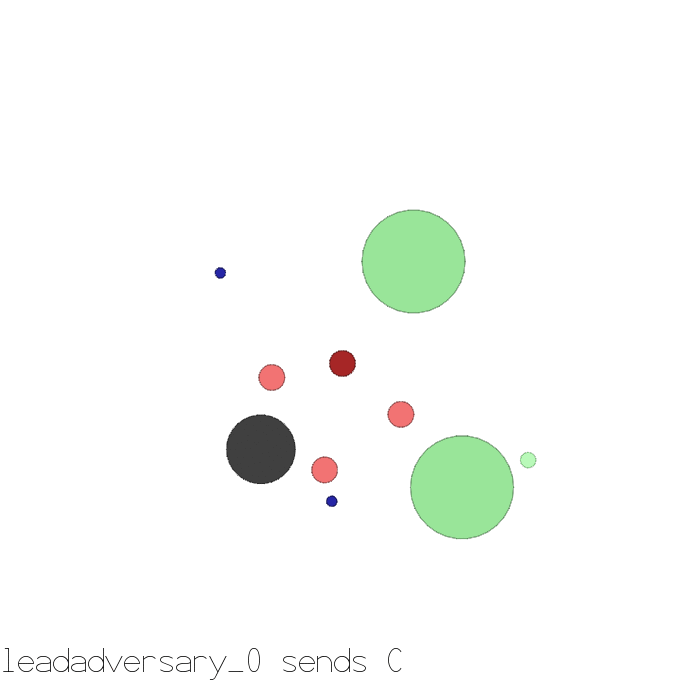
\includegraphics[trim=0cm 4.5cm 0cm 1cm, clip,width=0.9\linewidth]{figures/predator_prey.png}
  \caption[Screenshot of the Predator-Prey environment]{Screenshot of the Predator-Prey environment: \textbf{green agents} (cooperative) and \textbf{red agents} (adversaries). The green agents aim to collect food scattered throughout the environment while avoiding detection by the red agents. The environment includes \textbf{forest areas} that provide shelter; when a green agent enters a forest, it becomes partially or completely invisible to red agents. A red agent acts as a \textbf{leader} with enhanced observation abilities and can communicate with other red agents to coordinate their pursuit.}
  \label{fig:predator_prey}
\end{figure}

\subsubsection*{Warehouse Management}

The \textbf{Warehouse Management}~\cite{warehouse_management} environment models a grid-based logistics warehouse where multiple robots must collaborate to efficiently transport goods. This environment is inspired by industrial warehouse automation scenarios and provides an ideal test bed for evaluating task distribution, role specialization, and real-time coordination. This environment is illustrated in \autoref{fig:warehouse}\index{Warehouse Management}\index{Warehouse Management}.
%
% \begin{enumerate*}[label={\roman*)}, itemjoin={; \quad}]
\begin{itemize}
  \item \textbf{State space:} An $N \times M$ grid where each cell contains a robot, a product, a manufacturing machine, or a storage location. The system tracks agent positions, stock levels, and machine states
  \item \textbf{Observation space:} Each agent has a local view $V \times V$, allowing it to perceive nearby products, teammates, and machines
  \item \textbf{Action space:}
        \begin{enumerate*}[label={\roman*)}, itemjoin={; \quad}]
          \item Movement: \textquote{Up, Down, Left, Right}
          \item Interaction: \textquote{Pick up a product, drop off a product}.
        \end{enumerate*}
  \item \textbf{Reward structure:}
        \begin{enumerate*}[label={\roman*)}, itemjoin={; \quad}]
          \item Successful product delivery: $+10$
          \item Inefficient movement: $-1$ per unnecessary step
          \item Improper product handling: $-5$ for incorrect deliveries.
        \end{enumerate*}
  \item \textbf{Objective:} Transport raw materials to processing machines and deliver finished products to delivery locations.
        % \end{enumerate*}
\end{itemize}
%
\textbf{Organizational specifications:}
% \begin{enumerate*}[label={\roman*)}, itemjoin={; \quad}]
\begin{itemize}
  \item \textbf{Roles:} \textquote{Transporter, inventory manager}
  \item \textbf{Tasks:} Carriers transport products, while inventory managers oversee inventory levels.
  \item \textbf{Constraints:} Carriers must prioritize essential deliveries.
\end{itemize}
% \end{enumerate*}

\begin{figure}[h!]
\centering
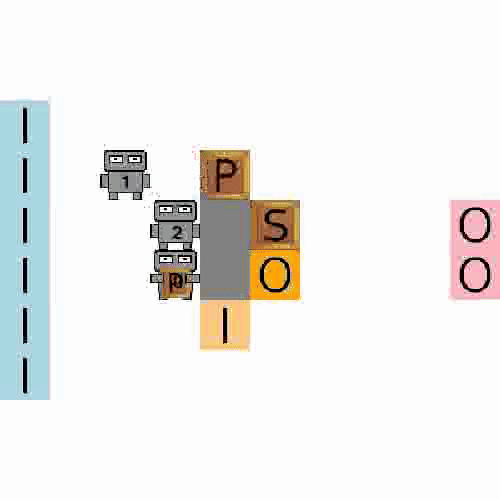
\includegraphics[trim=0cm 3cm 0cm 3cm, clip, width=0.9\linewidth]{figures/wm.png}
\caption[Screenshot of the Warehouse Management environment]{Screenshot of the Warehouse Management environment: agents can move up, down, left, and right. Multiple agents operate within a warehouse grid, performing tasks to process and deliver products. Agents can move in four directions (up, down, left, right) and interact with pick/drop zones when adjacent. The workflow includes: (i) collecting primary products from the pick/drop zones of the input conveyor (blue zones); (ii) transporting them to the pick/drop zones of the manufacturing machines (brown zones), where the primary products are transformed into a single secondary product according to a predefined manufacturing scheme; (iii) retrieval of the secondary products obtained and their delivery to the pick/place areas of the output conveyor (pink areas). For the operation to be successful, agents must coordinate their movements and actions to optimize throughput and efficiency within the warehouse.}
\label{fig:warehouse}
\end {figure}



\subsection{Description of the common instance of the experimentation protocol}

\paragraph{1. Initial configuration}

We use the \emph{PettingZoo} implementations of \phantom{X} \textbf{Overcooked-AI}, \textbf{Predator-Prey}, and \textbf{Warehouse Management} as \emph{real environments} in the sense of \textquote{CybMASDE}. Specifically, for a given environment, an instance of the game is launched in the background and exposed via a \acn{REST} adapter compliant with the \acn{API} of \textquote{CybMASDE} (attached observations, action masks, \emph{step}/\emph{reset}) . This gateway enables (i) the collection of traces for modeling (\textquote{\acn{MOD-AUT}}); (ii) \acn{MARL} training with organizational constraints; (iii) organizational analysis (\textbf{ANL}); (iv) transfer (\textbf{TRF}) to the standardized simulated executor.
For \textquote{\acn{MOD-AUT}}, a \emph{Joint-Observation Prediction Model} (\acn{JOPM}, \acn{VAE}+\acn{LSTM}) is trained on the collected histories (random policies and preliminary policies) in order to learn the dynamics $\langle o_{1:t},a_ {1:t} \rangle \mapsto o_{t+1}$ and a derived stop function. The reward function reconstructed from the traces is validated by cross-checking with the native reward of the environment. The observation/action label mapping ($l_o, l_a$) is defined to synchronize \textquote{PettingZoo} and \acn{MMA}, activate action masking and bonus/penalty injection by role. Training is based on \textquote{MARLlib}/\ textquote{RLlib} (default \textquote{MAPPO} profile, \textquote{Optuna} enabled), with fixed \textit{seeds} and 5 independent runs in accordance with \autoref{chap:experimental_framework}. The hardware resources are those presented \autoref{par:compute_conditions}; only the exceptions (episode length, log frequency) are specified in the results.

\paragraph{2 to 4. Definition of baselines}

For the three environments, we define a \textbf{default advanced baseline} and \textbf{alternative baselines} (ablations) that vary the \acn{MAMAD} activities, the \acn{MARL} algorithm, the mode of constraint integration, and their hardness, in order to isolate the contribution of each component (organizational guidance, modeling, analysis). We do not take into account specific metrics such as \emph{dishes served}/episode, collisions, inactive steps, time to performance plateau for Overcooked-AI, for example. \autoref{tab:non_cyberdefense_baselines} summarizes the experimental baselines planned for all three environments.


\begin{table*}[h!]
  \centering
  \caption{Synthetic baselines for non-cyberdefense-oriented environments.}
  \label{tab:non_cyberdefense_baselines}
  \renewcommand{\arraystretch}{1}
  \tiny
  \begin{tabularx}{\textwidth}{
      >{\raggedright\arraybackslash\hsize=0.3\hsize}X
      >{\raggedright\arraybackslash\hsize=0.15\hsize}X
      >{\raggedright\arraybackslash\hsize=0.15\hsize}X
      >{\raggedright\arraybackslash\hsize=0.3\hsize}X
    }
    \toprule
    \textbf{MAMAD activity profile} & \textbf{MARL algorithms} & \textbf{Organizational constraints (rigidity)} & \textbf{Comments}                                                                             \\
    \midrule
    % --- Profile A (Default) ---
    \multirow{3}{*}{\parbox{3.8cm}{\textbf{Profile A -- Default}                                                                                                                                                \\\acn{MOD-AUT};\;\acn{TRN-CON};\ ;\acn{ANL-AUT};\;\acn{TRF-AUT}}}
                                    & \acn{MAPPO}              & Yes (1.0)                                      & Action masking + role-based shaping (\acn{MMA}); \acn{JOPM} enabled for \acn{MOD-AUT}.        \\
                                    & \;\acn{MADDPG}           & Soft (0.5)                                     & Mitigated constraints: bonuses/penalties and partial masks; same pipeline as default.         \\
                                    & \acn{QMIX}               & None (0.0)                                     & \textit{Ablation}: \acn{TRN-UNC}, native environment reward, remains unchanged.               \\
    \hdashline
    % --- Profile B (Manual Analysis) ---
    \multirow{3}{*}{\parbox{3.8cm}{\textbf{Profile B -- Manual Analysis}                                                                                                                                        \\\acn{MOD-AUT};\;\acn{TRN-CON};\;\acn{ANL-MAN};\;\acn{TRF-AUT}}}
                                    & \acn{MAPPO}              & Yes (1.0)                                      & Manual configuration of \acn{TEMM}; rules/masks edited by hand.                               \\
                                    & \acn{COMA}               & Soft (0.5)                                     & Flexible guidance: reduced penalties; post-hoc verification by manually adjusted \acn {TEMM}. \\
                                    &                          & None (0.0)                                     & \acn{TRN-UNC}; \acn{TEMM} analysis only for explainability/diagnosis, without reinjection.    \\
    \hdashline
    % --- Profile C (Mainly manual cycle) ---
    \multirow{3}{*}{\parbox{3.8cm}{\textbf{Profile C -- Mainly manual cycle}                                                                                                                                    \\\acn{MOD-MAN}; \acn{TRN-CON}; \acn{ANL-MAN}; \acn{TRF-MAN}}}
                                    & \acn{IQL}                & Yes (1.0)                                      & \textquote{Handcrafted} environment; fixed hyperparameters; manual transfer and deployment.   \\
                                    & \acn{VDN}                & Soft (0.5)                                     & Soft constraints defined manually (roles/missions + softened scales).                         \\
                                    & \acn{MADDPG}             & None (0.0)                                     & \acn{TRN-UNC} entirely manual; zero organizational constraint hardness.                       \\
    \bottomrule
  \end{tabularx}
\end{table*}



\section{Experiments on the Company Infrastructure environment}
\textbf{Company Infrastructure}~\cite{cyberbattlesim}: a simulation of attacks and defenses on a network.

The \textbf{Company Infrastructure} environment is a simulation inspired by the CyberbatlleSim simulator~\cite{cyberbattlesim} and MITRE ATT\&CK~\cite{MITREATTACKWebsite}. This environment was developed with the \acn{Dec-POMDP} pre-specialized for cyber defense and with \acn {MCAS} integrated into \acn{CybMASDE}. It simulates a corporate network divided into subnetworks (EXT, DMZ, ACC, MAR, SRV) where \emph{cyber attack agents} and \emph{cyber defense agents} interact via pre/post-condition actions, according to a \emph{Dec-POMDP} formalism. The synthetic topology is illustrated in \autoref{fig:scenario_network_topology}, and the attack/defense paths are structured via an Attack–Defense tree (\autoref{fig:ADTree})\index {Company Infrastructure}.

% \begin{enumerate*}[label={\roman*)}, itemjoin={; \quad}]
\begin{itemize}
  \item \textbf{State space:} A set of discrete properties describing the state of network nodes (files, active services, versions, firewall rules, sessions, logs, agent knowledge). The topology includes:
        \begin{enumerate*}[label={\alph*)}, itemjoin={; \ }]
          \item \textbf{EXT}: two attacker workstations \textquote{At1, At2}
          \item \textbf{DMZ}: \textquote{\acn{WS}, \acn{ES}, \acn{VPN}, FTP}
          \item \textbf{ACC}: \textquote{E1, E2, CTO}
          \item \textbf{MAR}: \textquote{\acn{PS}, E3, \allowbreak \acn{TAB}}
          \item \textbf{SRV}: \textquote{\acn{API}, \acn{DB}, DC}.
        \end{enumerate*}
        Transitions modify all properties (addition/deletion/update) when the preconditions for action are met
  \item \textbf{Observation space:} Partial observations specific to each agent (relation $Obs$) such as file/log contents, command results, port scans, session states, detection alerts. Observations are returned after action is applied and depend on local visibility (sensors, privileges)
  \item \textbf{Action space:} Actions with \emph{preconditions} (conjunctions/disjunctions of properties) and \emph{postconditions} (writes to state), divided into broad families~:
        \begin{enumerate*}[label={\alph*)}, itemjoin={; \ }]
          \item \textbf{Attackers}: \textquote{Network/account reconnaissance}, \textquote{Exploiting service vulnerabilities}, \textquote{Privilege escalation}, \textquote{Lateral movement }, \textquote{Persistence (e.g., backdoor)}, \textquote{Data exfiltration (\acn{DB})}, \textquote{Spyware installation (\acn{PS})}
          \item \textbf{Defenders}: \textquote{Log detection (\acn{WS})}, \textquote{Privileged account management (\acn{PAM})}, \textquote{Command/argument monitoring (\acn{DB})}, \textquote{Traffic blocking/FW rules}, \textquote{Malicious session deletion}, \textquote{Service restoration}.
        \end{enumerate*}
  \item \textbf{Reward structure:} Function $R = Eval \circ Metrics$ evaluating status \& action using metrics (attack progress toward objectives, detections, deleted sessions, service integrity, etc.):
        \begin{enumerate*}[label={\alph*)}, itemjoin={; \ }]
          \item \textbf{Attackers}: progression bonus along the AD-tree ($+r_{\small step}$), ultimate objectives: \textquote{DB exfiltration} and \textquote{PS spyware} ($+R_{\small goal}$), penalties if detected/neutralized ($-\lambda_{\small det}$)
          \item \textbf{Defenders} : detection/prevention bonus ($+r_{\small det}$), session deletion ($+r_{\small purge}$), availability/integrity maintenance ($+r_{\small avail}$), penalties if attacker objectives achieved ($-\Lambda_{\small goal}$).
        \end{enumerate*}
  \item \textbf{Objective:} For \textbf{Attackers}, achieve \emph{DB Exfiltration} and \emph{Spyware PS} while minimizing detection; for \textbf{Defenders}, prevent/detect/neutralize these attack paths while maintaining critical services.
        % \end{enumerate*}
\end{itemize}

\medskip
\textbf{Organizational Specifications:} \emph{(Baseline)} no organizational constraints are imposed (\textquote{\acn{TRN-UNC}}), in order to provide a \emph{raw} reference for guided cyberdefense-oriented scenarios. \emph{(Optional variant, for ablative analyses)}:
% \begin{enumerate*}[label={\roman*)}, itemjoin= {; \quad}]
\begin{itemize}
  \item \textbf{Roles (ex.)}: \textquote{Attacker\_LateralMove}, \textquote{Attacker\_ExfilDB}, \textquote{Defender\_WS\_Monitor}, \textquote{Defender\_DB\_PAM}
  \item \textbf{Missions}: chain MITRE techniques by sub-objective (recon \textrightarrow{} exploitation \textrightarrow{} elevation \textrightarrow{} lateral movement \textrightarrow{} action on the objective) red side; detection \textrightarrow{} containment \textrightarrow{} eradication \textrightarrow{} recovery blue side
  \item \textbf{Constraints}: role-based permissions (action masking), minimum mission sequencing, conditional containment triggers (logs/\acn{IOC}).
\end{itemize}
% \end{enumerate*}

\begin{figure}[h!]
\centering
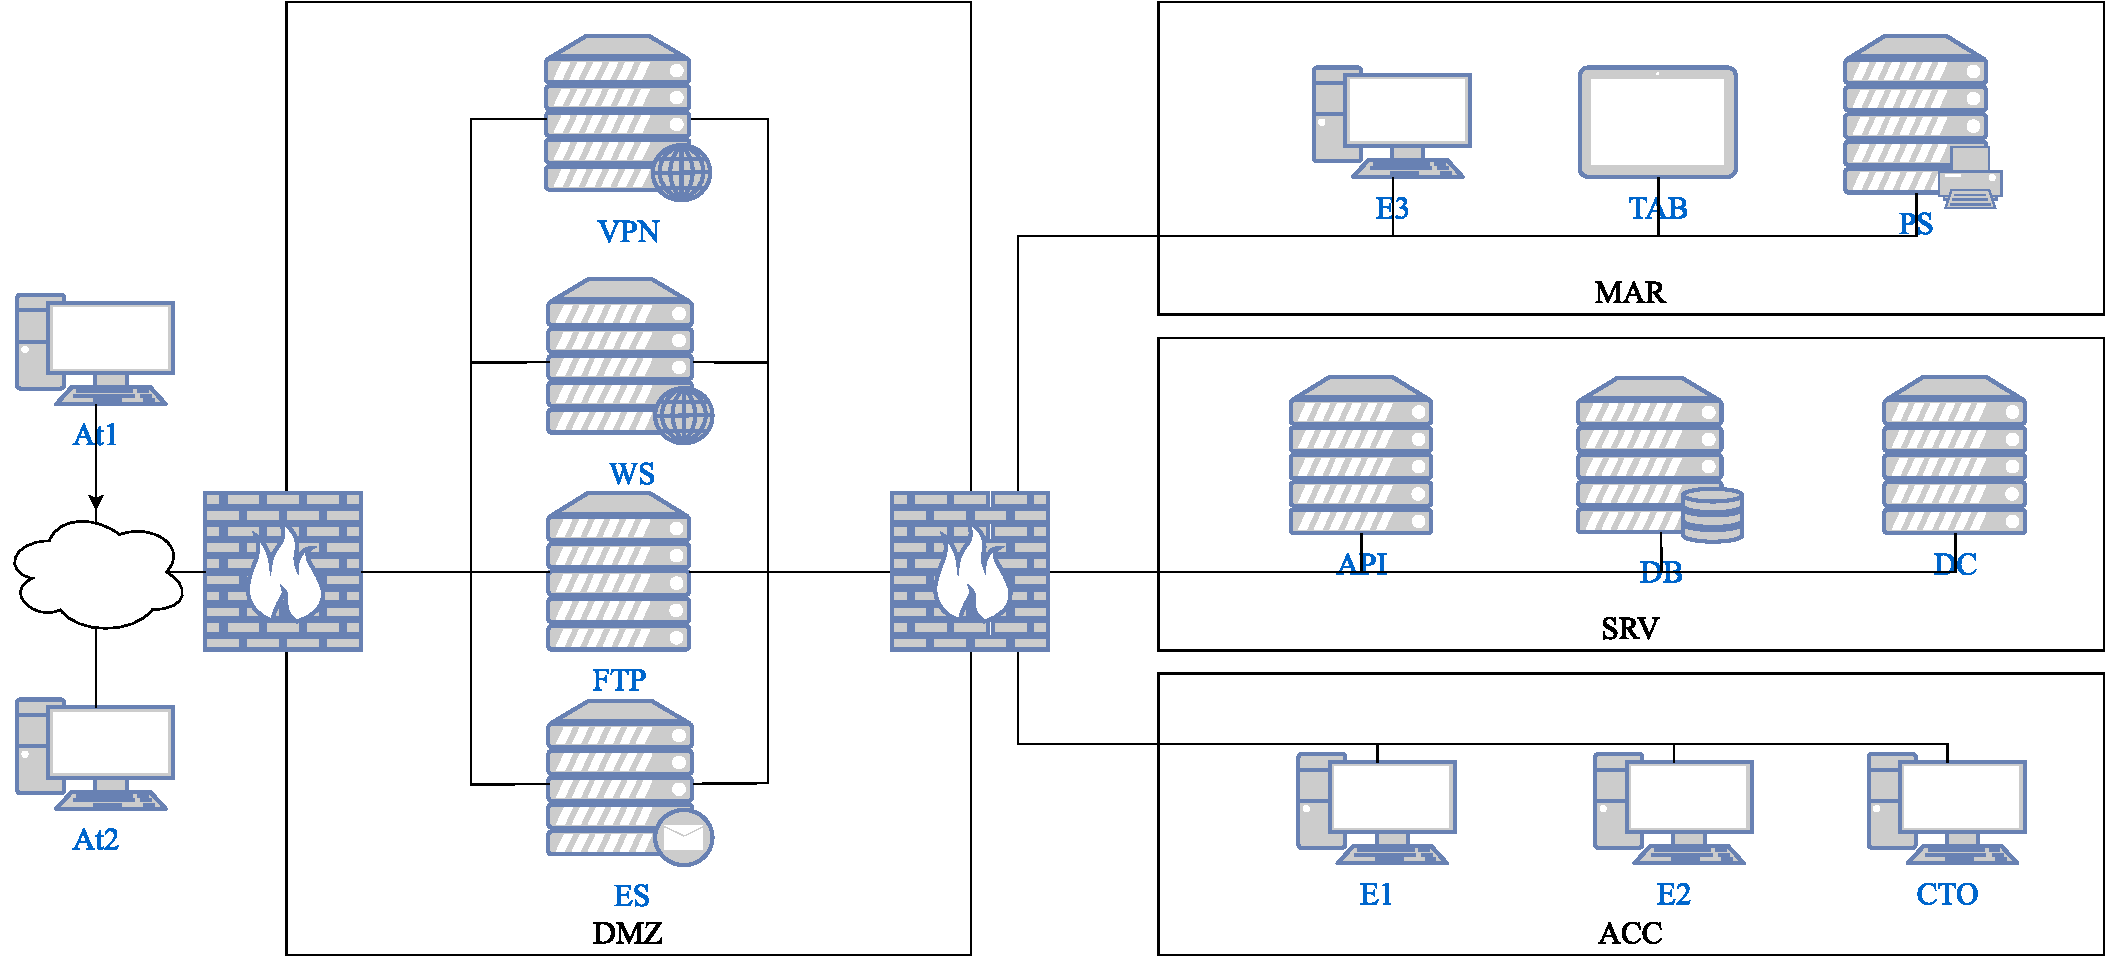
\includegraphics[width=\linewidth]{figures/topology.pdf}
\caption{Synthetic network topology: EXT, DMZ, ACC, MAR, SRV. Subnets are interconnected via implicit routers/firewalls.}
\label{fig:scenario_network_topology}
\end {figure}

\begin{figure}[h!]
  \centering
  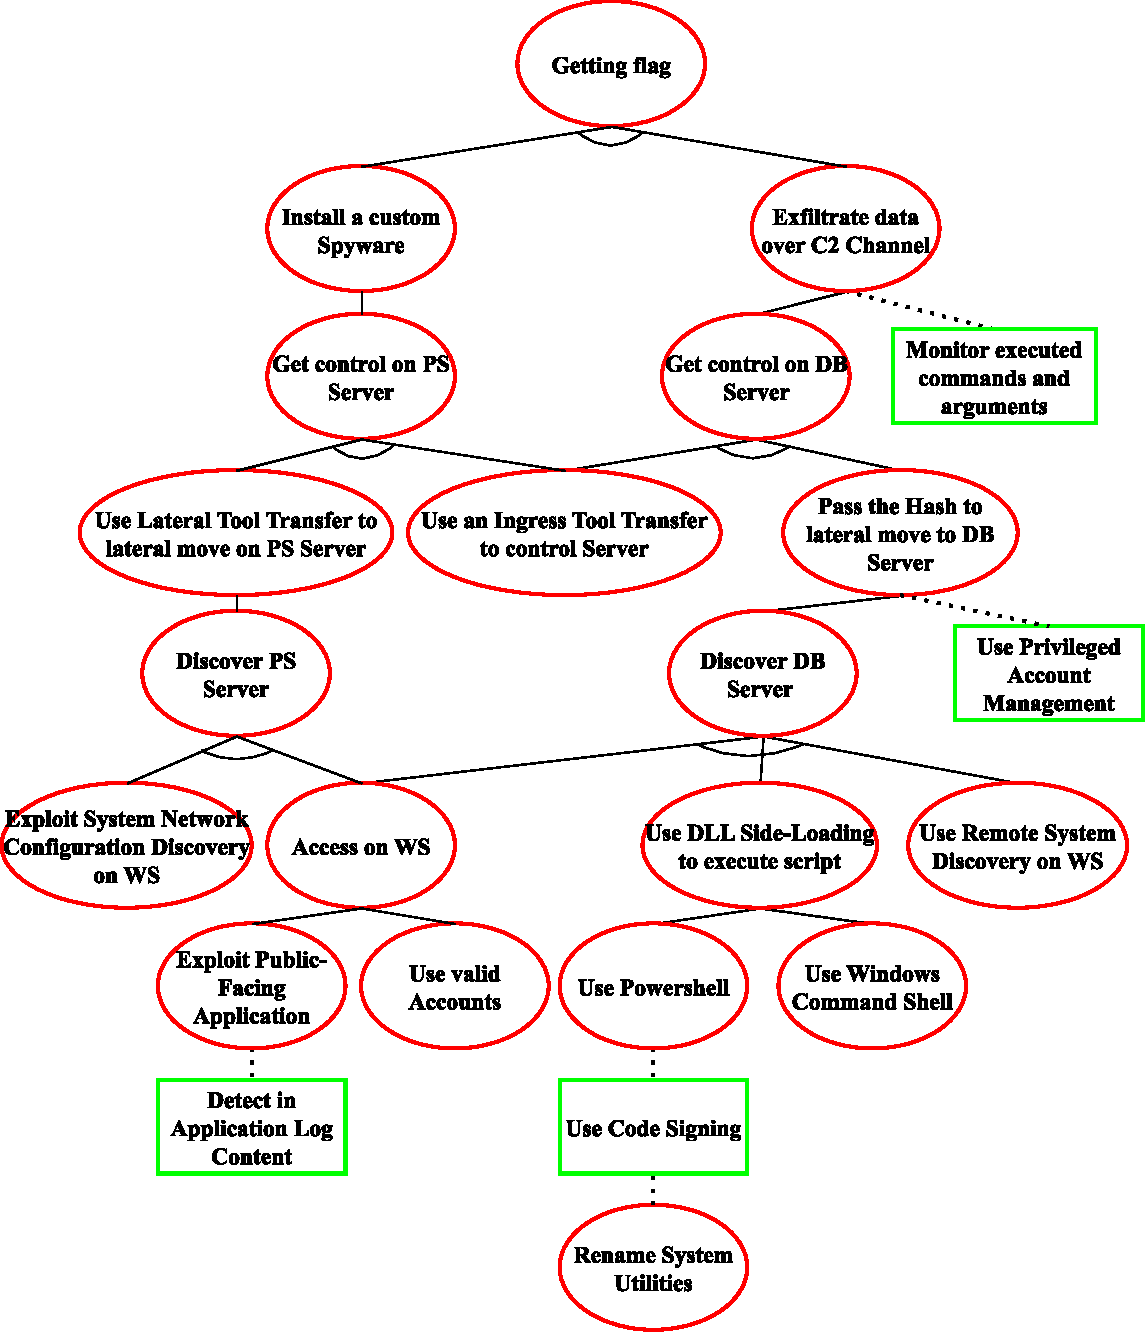
\includegraphics[width=0.86\linewidth]{figures/ADTree.pdf}
  \caption{Overview of the Attack–Defense (AD) tree structuring attack paths (MITRE tactics/techniques) and associated countermeasures. }
  \label{fig:ADTree}
\end{figure}


\subsection{Description of the experimental protocol instance}

\paragraph{1. Initial configuration}

We use the pre-specialized \emph{Dec-POMDP} model \textbf{Cyberdefense} and the \textbf{MCAS} simulator integrated into \textquote{CybMASDE}, exposed via a \acn{REST} adapter compliant with the \acn{API} of I/O \textquote{CybMASDE} (attached observations, action masks, \emph{step}/\emph{reset}). The \emph{Company Infrastructure} environment is therefore treated, on the pipeline side, exactly like non-Cyberdefense-oriented toy environments: (i) trace collection for automatic modeling (\textquote{\acn{MOD-AUT}} ); (ii) \acn{MARL} training with or without organizational constraints; (iii) organizational analysis (\textbf{ANL}); (iv) automatic transfer (\textquote{\acn{TRF-AUT}}) to the simulated executor.
\textbf{Justification:} no \textquote{\acn{TRF-MAN}} is required here, as the environment is not an instrumentation of a real system, but a natively compatible simulator (no \textquote{field gateway} to maintain).
For \textquote{\acn{MOD-AUT}}, a \acn{JOPM} (\acn{VAE}+\acn{LSTM}) is trained on histories combining random trajectories and preliminary \emph{red/blue} policies (progression in the \acn{AD}-tree, detections, quarantines). The \acn{JOPM} approximates the dynamics $\langle o_{1:t},a_{1:t} \rangle \ mapsto o_{t+1}$ and provides a derived stop function (objectives achieved, neutralization of malicious sessions, \emph{step-limit}). The reconstructed reward function is validated by cross-checking with native metrics (progress along the \acn{AD}-tree, service availability) . Training is based on \textquote{MARLlib}/\textquote{RLlib} (default \textquote{MAPPO} profile, but variants tested below), fixed seeds, and 5 independent runs as in \autoref{chap:experimental_framework}. The calculation conditions follow those presented in \autoref{par:compute_conditions}; only the exceptions (episode length, log frequency) are specified in the results.

\paragraph{2 to 4. Definition of baselines}

We define a \textbf{default advanced baseline} and \textbf{ablations} that vary (a) \acn{MAMAD} activities, (b) the \acn{MARL} algorithm, (c) the \emph{strictness} of organizational constraints: \emph{strong} (1.0), \emph{soft} (0.5), \emph{none} (0.0). All are based on \textquote{\acn{TRF-AUT}} (no \textquote{\acn{TRF-MAN}}, see justification above).

\begin{table*}[h!]
  \centering
  \caption {Synthetic baselines for Company Infrastructure.}
  \label{tab:baselines_company}
  \renewcommand{\arraystretch}{1}
  \tiny
  \begin{tabularx}{\textwidth}{
      >{\raggedright\arraybackslash\hsize=0.3\hsize}X
      >{\raggedright\arraybackslash\hsize=0.15\hsize}X
      >{\raggedright\arraybackslash\hsize=0.15\hsize}X
      > {\raggedright\arraybackslash\hsize=0.3\hsize}X
    }
    \toprule
    \textbf{MAMAD activity profile} & \textbf{MARL algorithms}            & \textbf{Organizational constraints (rigidity)} & \textbf{Comments}                                                                                                                   \\
    \midrule
    % --- Profile A (Default) ---
    \multirow{3}{*}{\parbox{3.8cm}{\textbf{Profile A -- Default}                                                                                                                                                                                                 \\
        \textquote{\acn{MOD-AUT}};\;\textquote{\acn{TRN-CON}};\;\textquote{\acn{ANL-AUT}};\;\textquote{\acn{TRF-AUT}}}}
                                    & \acn{MAPPO}, \acn{QMIX}, \acn{COMA} & Yes (1.0)                                      & Role-based masking (red/blue), \acn{AD}-tree aligned shaping (attack progress/detection/quarantine); \acn{JOPM} enabled.            \\
                                    & \acn{MAPPO}, \acn{QMIX}, \acn{COMA} & Soft (0.5)                                     & Same pipeline, mitigated penalties/bonuses; partial masks (expanded exploration).                                                   \\
                                    & \acn{MAPPO}, \acn{QMIX}             & None (0.0)                                     & \textit{Ablation} \acn{TRN-UNC}: native reward (state/metrics), no organizational guidance.                                         \\
    \hdashline
    % -- - Profile B (Manual Analysis) ---
    \multirow{3}{*}{\parbox{3.8cm}{\textbf{Profile B -- Manual Analysis}                                                                                                                                                                                         \\
        \textquote{\acn{MOD-AUT}};\;\textquote{\acn{TRN-CON}};\;\textquote{\acn{ANL-MAN}} (\acn{TEMM} parameterized);\; \textquote{\acn{TRF-AUT}}}}
                                    & \acn{MAPPO}, \acn{COMA}             & Yes (1.0)                                      & \acn{TEMM} set manually; rules/masks edited (sequencing recon$\rightarrow$exploitation$\rightarrow$\acn{LM}$\rightarrow$objective). \\
                                    & \acn{MAPPO}, \acn{COMA}             & Soft (0.5)                                     & Flexible guidance, post-hoc control by \acn{TEMM}.                                                                                  \\
                                    & \acn{MAPPO}                         & None (0.0)                                     & \acn{TRN-UNC}; \acn{TEMM} only for explainability/diagnosis (no rule reinjection).                                                  \\
    \hdashline
    % --- Profile C (Semi-manual cycle) ---
    \multirow{3}{*}{\parbox{3.8cm}{\textbf{Profile C -- Semi-manual cycle}                                                                                                                                                                                       \\
        \textquote{\acn{MOD-MAN}} (extended actions/props);\;\textquote{\acn{TRN-CON}} (manual hp); \;\textquote{\acn{ANL-MAN}};\;\textquote{\acn{TRF-AUT}}}}
                                    & \acn{IQL}, \acn{VDN}, \acn{QMIX}    & Yes (1.0)                                      & \textquote{Handcrafted} expansion of the action catalog (\acn{FW}, \acn{PAM}, persistence); fixed hyperparameters (not \acn{HPO}).  \\
                                    & \acn{IQL}, \acn{VDN}, \acn{QMIX}    & Soft (0.5)                                     & Manually defined soft constraints (log thresholds/\acn{IOC}, service priorities).                                                   \\
                                    & \acn{IQL}, \acn{VDN}                & None (0.0)                                     & Zero constraint hardness; useful for gauging the contribution of constraints and shaping.                                           \\
    \bottomrule
  \end{tabularx}
\end{table*}


\section{Experiments on the Kubernetes Microservices environment}


The \textbf{Kubernetes Microservices} environment is a \emph{real cluster} (1 \textit{worker} node: 8 vCPUs, 32 GB \acn{RAM}, 1 Gbps) used as the input environment for the MAMAD method. A schematic illustration of this cluster and its services is provided in \autoref{fig:k8s_microservices_real}. The cluster hosts an e-commerce web application composed of 4 chained microservices (API, Auth, Products, Orders) orchestrated via Kubernetes. Each service is deployed in a pod with a variable number of replicas (1 to 5). The cluster is ({API}, Auth, Products, Orders) orchestrated via Kubernetes. Each service is deployed in a \emph{pod} with a variable number of replicas (1 to 5). The cluster is monitored in real time via Prometheus/Grafana, collecting metrics such as \acn{CPU}/memory usage, request rate, latency, queues, and pod status. Stress test scenarios are applied to simulate real-world conditions: bottlenecks (increased traffic), DDoS attacks (malicious traffic), pod failures (simulated via \textquote{kubectl delete pod}), and resource contention (\acn {CPU}/memory). The goal is to evaluate the agents' ability to maintain the cluster's operational resilience by dynamically adapting resources and responding to incidents. A summary illustration of this type of scenario is provided in \autoref{fig:k8s_cluster_graph_intro}\index{Kubernetes Microservices}.


% \begin{enumerate*}[label={\roman*)}, itemjoin={;\quad}]
\begin{itemize}

  \item \textbf{State space:} current state of the actual cluster and the 4 chained services \((i \in \{1..4\})\):
        \(
        s = \{\text{replicas}^i,\,
        U_{\text{cpu}}^i, U_{\text{mem}}^i,\,
        T_{\text{in}}^i, T_{\text{out}}^i,\ ,
        Q_{\text{pending}}^i,\,
        S_{\text{status}}^{i,\text{pods}},\,
        P_{\text{priority}}^i\}_{i=1..4}
        \)
        and global aggregates (average latency \(L_{\text{avg}}\), request rate \(R_{\text{rate}}\), availability)

  \item \textbf{Observation space:} partial \emph{actual} observation (\acn{Dec-POMDP}) obtained via the Kubernetes/metrics collection \acn{API}. It is \emph{role-specific}:
        \begin{enumerate*}[label={}, itemjoin={;\,}]
          \item bottlenecks: \(Q_{\text{pending}}^i, T_{\text{in}}^i/T_{\text{out}}^i\)
          \item \phantom{XXX} DDoS: \(R_{\text{rate}}, \Delta T, L_{\text{avg}}\)
          \item failures: \(S_{\text{status}}^{i,\text{pods}}, F_{\text{fail}}^i\)
          \item resources: \(U_{\text{cpu}}^i, U_{\text{mem}}^i, P_{\text{priority}}^i\)
        \end{enumerate*}

  \item \textbf{Scope of action:} \emph{actual actions} applied to the cluster via the Kubernetes API:
        \begin{enumerate*}[label={\roman*)}, itemjoin={;\quad}]
          \item \emph{Targeted scaling}: \textquote{scale\_up}(i), \textquote{scale\_down} (i)
          \item \emph{DDoS management}: \textquote{rate\_limit\_ingress}(i), \textquote{isolate\_service}(i)
          \item \emph{Failure recovery}: \textquote{restart\_failed\_pod}(i), \textquote{reschedule\_pod}(i)
          \item \emph{Resource arbitration}: \textquote{throttle\_low\_prio}(i), \textquote{rebalance\_quota}(i)
        \end{enumerate*}

  \item \textbf{Reward structure:} reward \emph{calculated based on actual telemetry} (QoS/resilience):
        \[
          R_{\text{global}}=
          \text{SuccessRate} -w_2\cdot\text{DownTime} -w_3\cdot L_{\text{avg}} -w_4\cdot \text{Resilience} -w_5\cdot \text{Pending} -w_6\cdot \text{Pending\_Time} -w_7\cdot \text{Pending\_Time} -w_8\cdot \text{Pending\_Time} -w_9\cdot \text{Pending\_Time} -w_10\cdot \text{Pending\_Time} -w
          {SuccessRate}
          -w_2\cdot\overline{Q_{\text{pending}}}
          -w_3\cdot L_{\text{avg}}
          -w_4\cdot \text{DownTime}
          -w_5\cdot \text{OverProvision},
        \]
        supplemented by sub-rewards per role:
        \begin{gather*}
          R_{\text{bottleneck}}=-\sum_i Q_{\text{pending}}^i \\
          R_{\text{ddos}}=-(\text{Downtime}\cdot w_d+L_{\text{avg}}\cdot w_l) \\
          R_{\text{failure}}=-\sum_i T_{\text{downtime}}^i \\
          R_{\text{resource}}=-\sum_{i\in\text{Critical}}(U_{\text{cpu}}^i+U_{\text{mem}}^i)
        \end{gather*}

  \item \textbf{Objective:} maximize the \emph{operational resilience} of the actual cluster (high success rate, low latency/queues, maximum availability) under 5 scenarios: bottlenecks, DDoS, pod failures, resource contention, \emph{mixed}

        % \end{enumerate*}
\end{itemize}



\noindent\textbf{Organizational specifications:}
% \begin{enumerate*}[label={\roman*)}, itemjoin={;\quad}]
\begin {itemize}
\item \textbf{Roles:} \textquote{Bottleneck Manager}, \textquote{DDoS Manager}, \textquote{Outage Manager}, \textquote{Resource Manager}
\item \textbf{Tasks:}
\(\langle\)minimize \(Q_{\text{pending}}^i\)\(\rangle\);
\(\langle\)detect/isolate DDoS and reduce downtime/latency\(\rangle\);
\(\langle\)\(\downarrow T_{\text{downtime}}\) through rapid recovery\(\rangle\);
\(\langle\)prioritize critical services under \(U_{\text{cpu/mem}}\) constraint\(\rangle\)
\item \textbf{Constraints:}
(a) \emph{deontic} by role (e.g., only \textquote{DDoS Manager} can \textquote{isolate\_ \allowbreak service});
(b) \emph{segregation of responsibilities} (avoid contradictory \textquote{scale\_up});
(c) \emph{QoS safeguards} (\(Q_{\text{pending}}^i<Q_{\text{threshold}}, U_{\text{cpu}}^{\text{total}}<U_{\text{threshold}}\));
(d) two integration modes during training: \textit{hard constraints} (action masking) vs. \textit{soft constraints} (reward shaping)
% \end{enumerate*}
\end{itemize}

\medskip
\noindent\textit{Note (specificity \textquote{real}):}
% \begin{enumerate*}[label={--}, itemjoin={\quad}]
\begin{itemize}
  \item \textsc{MOD/TRN} on digital twin derived from real cluster traces;
  \item \textsc{TRF}: deployment of policies learned on the cluster via the Kubernetes API; {API};
  \item operational security: bounded actions (quotas/limits), rollbacks, and rate limiting to preserve QoS.
        % \end{enumerate*}
\end{itemize}

\begin{figure}[h!]
  \centering
  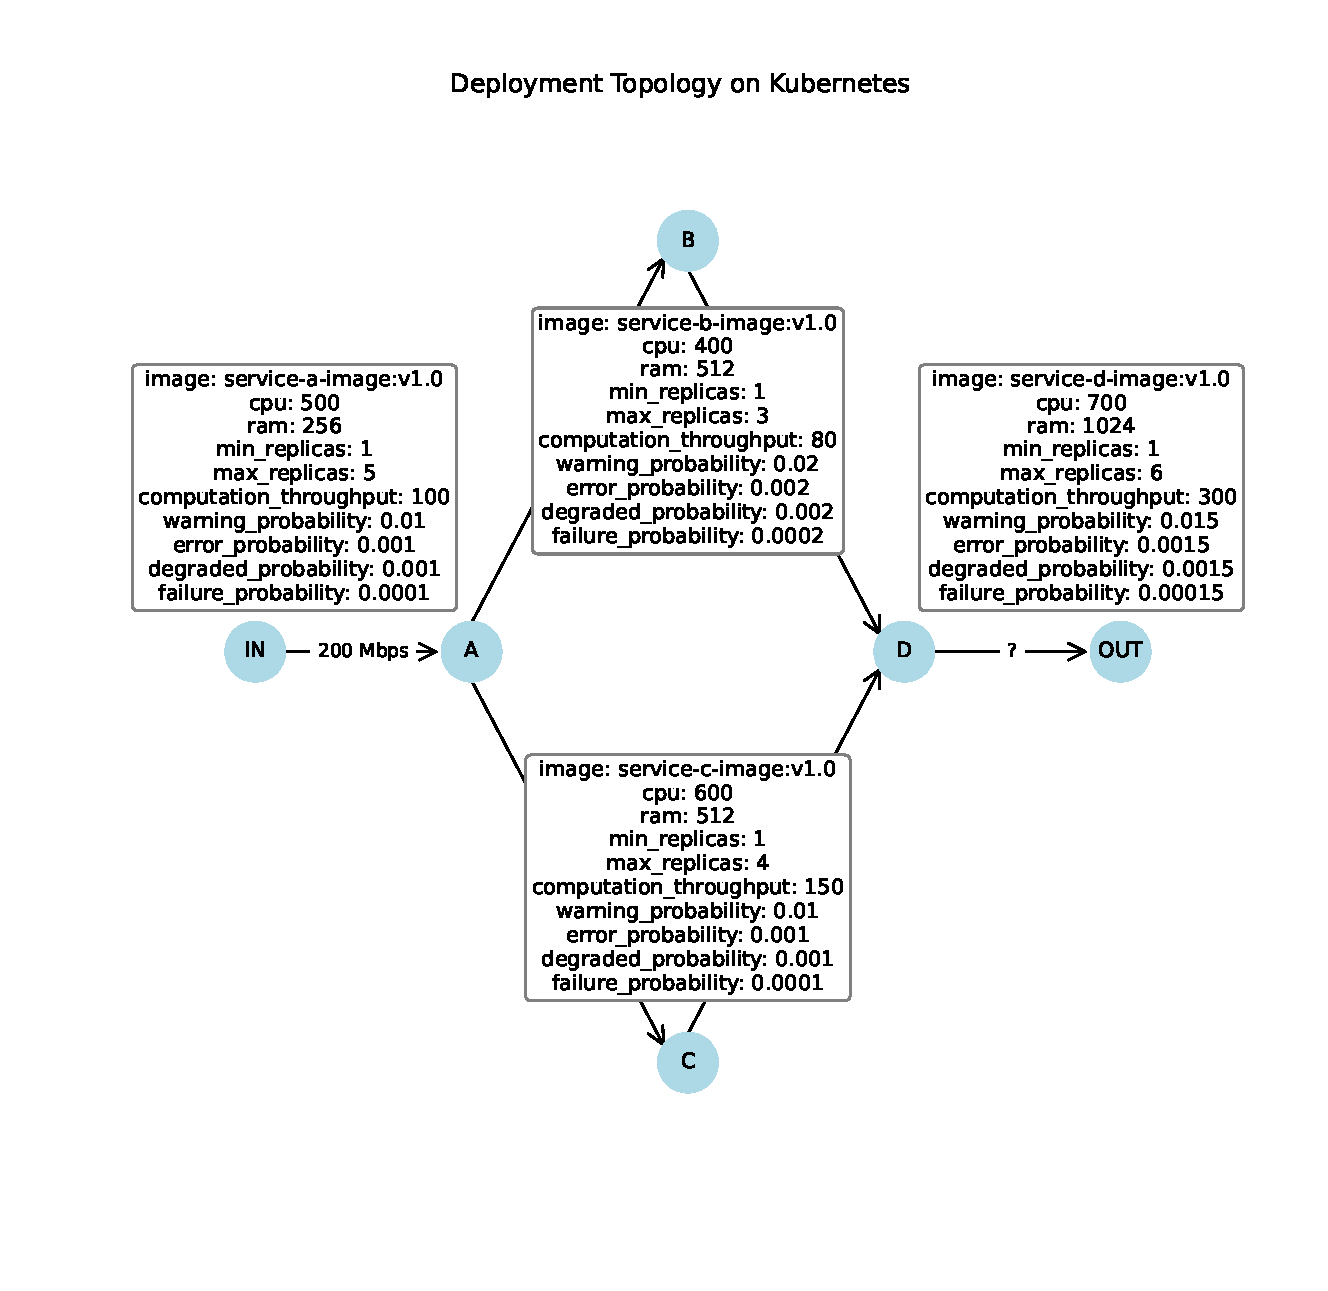
\includegraphics[trim=1.8cm 3.3cm 1.25cm 3.5cm, clip, width=\linewidth]{figures/k8s_cluster_graph.pdf}
  \caption{Real cluster \textquote{Chained services} (4 services) and levers of action exposed to CybMASDE/MAMAD via the Kubernetes API.}
  \label{fig:k8s_microservices_real}
\end{figure}

\begin{figure}[h!]
  \centering
  \hspace{-0.4cm}
  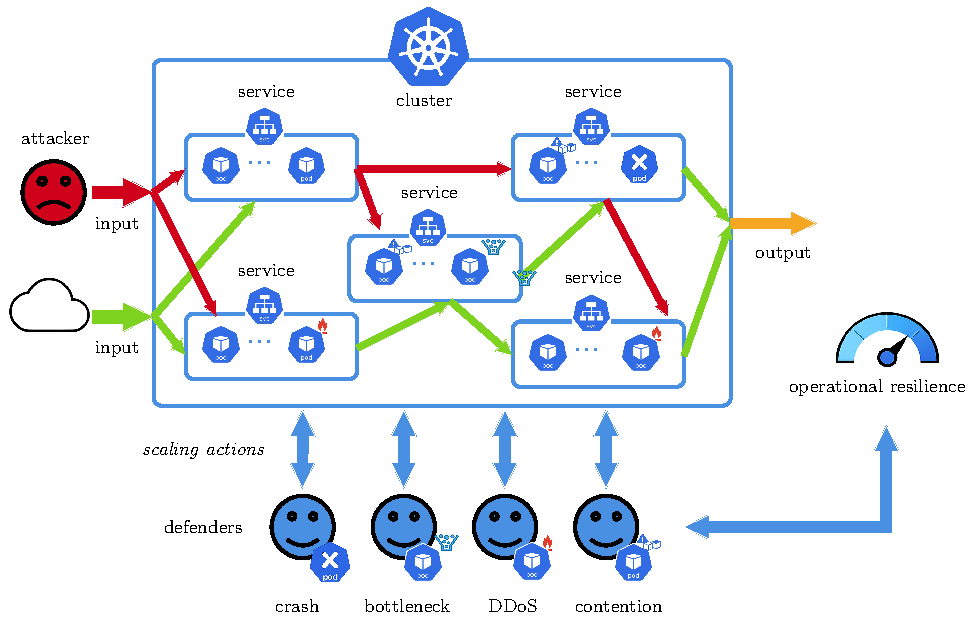
\includegraphics[trim=0cm 0cm 0cm 0cm, clip, width=\textwidth]{figures/scenario_introduction.pdf}
  \caption[An abstract view of the Kubernetes cluster scenario]{An abstract view of the Kubernetes cluster scenario where each service runs in pods managed by \textit{Deployments} and can be dynamically replicated. Defender agents with specific roles (e.g., \textit{DDoS detector}, \textit{resource manager}, \textit{bottleneck manager}, \textit{failure manager}) continuously monitor key metrics (latency, pending requests, incoming/outgoing traffic, pod states, \acn{CPU}/memory usage) and apply via the \ acn{API} to adjust replicas, isolate affected services, or restart failed components. The illustration highlights four types of disruptions targeting the chain (\textit{bottleneck}, \textit{contention} (resource conflict), \textit{crash} (pod failure), and \textit{DDoS}/massive injections), as well as pod compromises. Agents must detect anomalies, isolate/segment compromised components, and reallocate resources to preserve overall operational resilience (availability, throughput, latency) and minimize the impact on end users.}
  \label{fig:k8s_cluster_graph_intro}
\end{figure}


\subsection{Description of the experimental protocol instance}

\paragraph{1. Initial configuration}

We operate \emph{on the actual cluster} (no command line simulation playing the role of the \textquote{actual environment}). The cluster (\textbf{\acn{VM} 8~vCPU, 32 GB \acn{RAM}, 1 Gbps}) hosts the e-commerce application (4 microservices in a chain). Telemetry is collected by \textit{Prometheus} and visualized via \textit{Grafana}. \textquote{CybMASDE}/\textquote{KARMA} interfaces with the Kubernetes \acn{API} to \textit {observe} the status and \textit{act} (scaling, isolation, restart). A \textbf{digital twin} is built from the traces to train the policies offline, which are then \textbf{transferred} and \textit{closed in a loop} on the cluster (iterative learning by refreshing traces).

\begin{figure}[h!]
  \centering
  \resizebox{\textwidth}{!}{%
    


\tikzset{every picture/.style={line width=0.75pt}} %set default line width to 0.75pt        

\begin{tikzpicture}[x=0.75pt,y=0.75pt,yscale=-1.2,xscale=1.2]
%uncomment if require: \path (0,1414); %set diagram left start at 0, and has height of 1414

%Straight Lines [id:da5609883377896374] 
\draw [color={rgb, 255:red, 74; green, 144; blue, 226 }  ,draw opacity=1 ][line width=2.25]    (317.22,111.13) -- (360.07,111.13) ;
\draw [shift={(365.07,111.13)}, rotate = 180] [fill={rgb, 255:red, 74; green, 144; blue, 226 }  ,fill opacity=1 ][line width=0.08]  [draw opacity=0] (5.72,-2.75) -- (0,0) -- (5.72,2.75) -- cycle    ;
%Image [id:dp9396292457736715] 
\draw (106.77,60.95) node  {
\includegraphics[width=18.66pt,height=18.36pt]{figures/karma_architecture/pod.png}};
%Image [id:dp3874378335758297] 
\draw (145.86,60.95) node  {
\includegraphics[width=18.66pt,height=18.36pt]{figures/karma_architecture/pod.png}};
%Shape: Rectangle [id:dp4562827234223257] 
\draw  [color={rgb, 255:red, 74; green, 144; blue, 226 }  ,draw opacity=1 ][line width=1.5]  (89,28.36) .. controls (89,25.6) and (91.24,23.36) .. (94,23.36) -- (255,23.36) .. controls (257.76,23.36) and (260,25.6) .. (260,28.36) -- (260,132) .. controls (260,134.76) and (257.76,137) .. (255,137) -- (94,137) .. controls (91.24,137) and (89,134.76) .. (89,132) -- cycle ;
%Image [id:dp9455935833751838] 
\draw (172.5,16.24) node  {
\includegraphics[width=18.66pt,height=18.36pt]{figures/karma_architecture/kubernetes.png}};
%Shape: Rectangle [id:dp9564725691593288] 
\draw  [color={rgb, 255:red, 74; green, 144; blue, 226 }  ,draw opacity=1 ][line width=1.5]  (92.55,50.21) .. controls (92.55,47.45) and (94.79,45.21) .. (97.55,45.21) -- (155.08,45.21) .. controls (157.84,45.21) and (160.08,47.45) .. (160.08,50.21) -- (160.08,70.81) .. controls (160.08,73.57) and (157.84,75.81) .. (155.08,75.81) -- (97.55,75.81) .. controls (94.79,75.81) and (92.55,73.57) .. (92.55,70.81) -- cycle ;
%Image [id:dp9120856447688912] 
\draw (126.32,39.97) node  {
\includegraphics[width=18.66pt,height=18.36pt]{figures/karma_architecture/node.png}};
%Image [id:dp5738167237736518] 
\draw (106.77,119.52) node  {
\includegraphics[width=18.66pt,height=18.36pt]{figures/karma_architecture/pod.png}};
%Image [id:dp2199681121060142] 
\draw (145.86,119.52) node  {
\includegraphics[width=18.66pt,height=18.36pt]{figures/karma_architecture/pod.png}};
%Shape: Rectangle [id:dp12159705904547402] 
\draw  [color={rgb, 255:red, 74; green, 144; blue, 226 }  ,draw opacity=1 ][line width=1.5]  (92.55,108.78) .. controls (92.55,106.02) and (94.79,103.78) .. (97.55,103.78) -- (155.08,103.78) .. controls (157.84,103.78) and (160.08,106.02) .. (160.08,108.78) -- (160.08,129.38) .. controls (160.08,132.14) and (157.84,134.38) .. (155.08,134.38) -- (97.55,134.38) .. controls (94.79,134.38) and (92.55,132.14) .. (92.55,129.38) -- cycle ;
%Image [id:dp37768653229718074] 
\draw (126.32,98.54) node  {
\includegraphics[width=18.66pt,height=18.36pt]{figures/karma_architecture/node.png}};
%Shape: Rectangle [id:dp20840815212238661] 
\draw  [color={rgb, 255:red, 74; green, 144; blue, 226 }  ,draw opacity=1 ][line width=1.5]  (264,28.36) .. controls (264,25.6) and (266.24,23.36) .. (269,23.36) -- (411.78,23.36) .. controls (414.54,23.36) and (416.78,25.6) .. (416.78,28.36) -- (416.78,132) .. controls (416.78,134.76) and (414.54,137) .. (411.78,137) -- (269,137) .. controls (266.24,137) and (264,134.76) .. (264,132) -- cycle ;
%Straight Lines [id:da9232180983272227] 
\draw [color={rgb, 255:red, 74; green, 144; blue, 226 }  ,draw opacity=1 ][line width=2.25]    (164,112) -- (201,112) ;
\draw [shift={(206,112)}, rotate = 180] [fill={rgb, 255:red, 74; green, 144; blue, 226 }  ,fill opacity=1 ][line width=0.08]  [draw opacity=0] (5.72,-2.75) -- (0,0) -- (5.72,2.75) -- cycle    ;
%Straight Lines [id:da6082715106712999] 
\draw [color={rgb, 255:red, 74; green, 144; blue, 226 }  ,draw opacity=1 ][line width=2.25]    (180,90.22) -- (167,90.22) ;
\draw [shift={(162,90.22)}, rotate = 360] [fill={rgb, 255:red, 74; green, 144; blue, 226 }  ,fill opacity=1 ][line width=0.08]  [draw opacity=0] (5.72,-2.75) -- (0,0) -- (5.72,2.75) -- cycle    ;
%Straight Lines [id:da30764510910060716] 
\draw [color={rgb, 255:red, 74; green, 144; blue, 226 }  ,draw opacity=1 ][line width=2.25]    (210,72) -- (199,72) ;
\draw [shift={(194,72)}, rotate = 360] [fill={rgb, 255:red, 74; green, 144; blue, 226 }  ,fill opacity=1 ][line width=0.08]  [draw opacity=0] (5.72,-2.75) -- (0,0) -- (5.72,2.75) -- cycle    ;
%Straight Lines [id:da5394403186779959] 
\draw [color={rgb, 255:red, 74; green, 144; blue, 226 }  ,draw opacity=1 ][line width=2.25]    (178,56.22) -- (167,56.22) ;
\draw [shift={(162,56.22)}, rotate = 360] [fill={rgb, 255:red, 74; green, 144; blue, 226 }  ,fill opacity=1 ][line width=0.08]  [draw opacity=0] (5.72,-2.75) -- (0,0) -- (5.72,2.75) -- cycle    ;
%Straight Lines [id:da6399475815904785] 
\draw [color={rgb, 255:red, 74; green, 144; blue, 226 }  ,draw opacity=1 ][line width=2.25]    (272,72) -- (235,72) ;
\draw [shift={(230,72)}, rotate = 360] [fill={rgb, 255:red, 74; green, 144; blue, 226 }  ,fill opacity=1 ][line width=0.08]  [draw opacity=0] (5.72,-2.75) -- (0,0) -- (5.72,2.75) -- cycle    ;
%Straight Lines [id:da24320102833940327] 
\draw [color={rgb, 255:red, 74; green, 144; blue, 226 }  ,draw opacity=1 ][line width=2.25]    (267,112) -- (230,112) ;
\draw [shift={(272,112)}, rotate = 180] [fill={rgb, 255:red, 74; green, 144; blue, 226 }  ,fill opacity=1 ][line width=0.08]  [draw opacity=0] (5.72,-2.75) -- (0,0) -- (5.72,2.75) -- cycle    ;
%Shape: Rectangle [id:dp9149123987409296] 
\draw  [color={rgb, 255:red, 255; green, 255; blue, 255 }  ,draw opacity=1 ][fill={rgb, 255:red, 255; green, 255; blue, 255 }  ,fill opacity=1 ] (328.83,106.67) -- (353.11,106.67) -- (353.11,114) -- (328.83,114) -- cycle ;
%Image [id:dp7127891043436136] 
\draw (341.68,109.47) node  {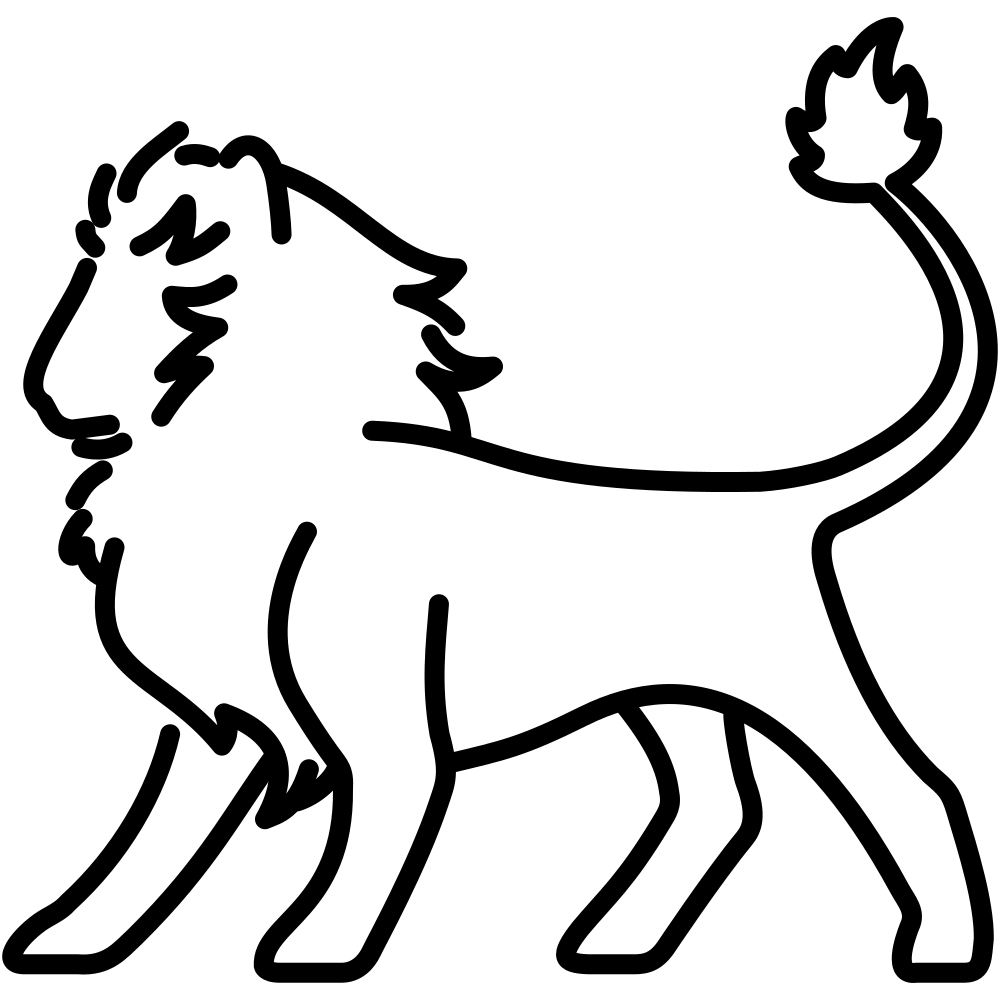
\includegraphics[width=14.57pt,height=15.21pt]{figures/karma_architecture/pettingzoo.png}};
%Straight Lines [id:da5757027637146572] 
\draw [color={rgb, 255:red, 74; green, 144; blue, 226 }  ,draw opacity=1 ][line width=2.25]    (357.9,41) -- (364.9,41) ;
\draw [shift={(352.9,41)}, rotate = 0] [fill={rgb, 255:red, 74; green, 144; blue, 226 }  ,fill opacity=1 ][line width=0.08]  [draw opacity=0] (5.72,-2.75) -- (0,0) -- (5.72,2.75) -- cycle    ;
%Straight Lines [id:da29364722138505184] 
\draw [color={rgb, 255:red, 74; green, 144; blue, 226 }  ,draw opacity=1 ][line width=2.25]    (390.99,97.77) -- (390.99,57.25) ;
\draw [shift={(390.99,52.25)}, rotate = 90] [fill={rgb, 255:red, 74; green, 144; blue, 226 }  ,fill opacity=1 ][line width=0.08]  [draw opacity=0] (5.72,-2.75) -- (0,0) -- (5.72,2.75) -- cycle    ;
%Straight Lines [id:da5470457469462804] 
\draw [color={rgb, 255:red, 74; green, 144; blue, 226 }  ,draw opacity=1 ][line width=2.25]    (390.9,71) -- (325.9,71) ;
\draw [shift={(320.9,71)}, rotate = 360] [fill={rgb, 255:red, 74; green, 144; blue, 226 }  ,fill opacity=1 ][line width=0.08]  [draw opacity=0] (5.72,-2.75) -- (0,0) -- (5.72,2.75) -- cycle    ;
%Shape: Rectangle [id:dp8476965567779329] 
\draw  [color={rgb, 255:red, 255; green, 255; blue, 255 }  ,draw opacity=1 ][fill={rgb, 255:red, 255; green, 255; blue, 255 }  ,fill opacity=1 ] (378.41,65.11) -- (397.83,65.11) -- (397.83,92) -- (378.41,92) -- cycle ;
%Shape: Smiley Face [id:dp8656850497140396] 
\draw  [fill={rgb, 255:red, 255; green, 255; blue, 255 }  ,fill opacity=1 ][line width=0.75]  (380.35,69.4) .. controls (380.35,67.3) and (382.09,65.6) .. (384.24,65.6) .. controls (386.38,65.6) and (388.12,67.3) .. (388.12,69.4) .. controls (388.12,71.5) and (386.38,73.2) .. (384.24,73.2) .. controls (382.09,73.2) and (380.35,71.5) .. (380.35,69.4) -- cycle ; \draw  [fill={rgb, 255:red, 255; green, 255; blue, 255 }  ,fill opacity=1 ][line width=0.75]  (382.53,68.11) .. controls (382.53,67.9) and (382.7,67.73) .. (382.92,67.73) .. controls (383.13,67.73) and (383.31,67.9) .. (383.31,68.11) .. controls (383.31,68.32) and (383.13,68.49) .. (382.92,68.49) .. controls (382.7,68.49) and (382.53,68.32) .. (382.53,68.11) -- cycle ; \draw  [fill={rgb, 255:red, 255; green, 255; blue, 255 }  ,fill opacity=1 ][line width=0.75]  (385.17,68.11) .. controls (385.17,67.9) and (385.34,67.73) .. (385.56,67.73) .. controls (385.77,67.73) and (385.95,67.9) .. (385.95,68.11) .. controls (385.95,68.32) and (385.77,68.49) .. (385.56,68.49) .. controls (385.34,68.49) and (385.17,68.32) .. (385.17,68.11) -- cycle ; \draw  [line width=0.75]  (382.29,70.92) .. controls (383.59,71.94) and (384.88,71.94) .. (386.18,70.92) ;
%Shape: Smiley Face [id:dp9163740789669144] 
\draw  [fill={rgb, 255:red, 255; green, 255; blue, 255 }  ,fill opacity=1 ][line width=0.75]  (392.01,69.4) .. controls (392.01,67.3) and (393.75,65.6) .. (395.89,65.6) .. controls (398.04,65.6) and (399.78,67.3) .. (399.78,69.4) .. controls (399.78,71.5) and (398.04,73.2) .. (395.89,73.2) .. controls (393.75,73.2) and (392.01,71.5) .. (392.01,69.4) -- cycle ; \draw  [fill={rgb, 255:red, 255; green, 255; blue, 255 }  ,fill opacity=1 ][line width=0.75]  (394.18,68.11) .. controls (394.18,67.9) and (394.36,67.73) .. (394.57,67.73) .. controls (394.79,67.73) and (394.96,67.9) .. (394.96,68.11) .. controls (394.96,68.32) and (394.79,68.49) .. (394.57,68.49) .. controls (394.36,68.49) and (394.18,68.32) .. (394.18,68.11) -- cycle ; \draw  [fill={rgb, 255:red, 255; green, 255; blue, 255 }  ,fill opacity=1 ][line width=0.75]  (396.82,68.11) .. controls (396.82,67.9) and (397,67.73) .. (397.21,67.73) .. controls (397.43,67.73) and (397.6,67.9) .. (397.6,68.11) .. controls (397.6,68.32) and (397.43,68.49) .. (397.21,68.49) .. controls (397,68.49) and (396.82,68.32) .. (396.82,68.11) -- cycle ; \draw  [line width=0.75]  (393.95,70.92) .. controls (395.24,71.94) and (396.54,71.94) .. (397.83,70.92) ;
%Shape: Smiley Face [id:dp8186451078369623] 
\draw  [fill={rgb, 255:red, 255; green, 255; blue, 255 }  ,fill opacity=1 ][line width=0.75]  (386.18,77.44) .. controls (386.18,75.34) and (387.92,73.64) .. (390.06,73.64) .. controls (392.21,73.64) and (393.95,75.34) .. (393.95,77.44) .. controls (393.95,79.54) and (392.21,81.24) .. (390.06,81.24) .. controls (387.92,81.24) and (386.18,79.54) .. (386.18,77.44) -- cycle ; \draw  [fill={rgb, 255:red, 255; green, 255; blue, 255 }  ,fill opacity=1 ][line width=0.75]  (388.36,76.15) .. controls (388.36,75.94) and (388.53,75.77) .. (388.74,75.77) .. controls (388.96,75.77) and (389.13,75.94) .. (389.13,76.15) .. controls (389.13,76.36) and (388.96,76.53) .. (388.74,76.53) .. controls (388.53,76.53) and (388.36,76.36) .. (388.36,76.15) -- cycle ; \draw  [fill={rgb, 255:red, 255; green, 255; blue, 255 }  ,fill opacity=1 ][line width=0.75]  (391,76.15) .. controls (391,75.94) and (391.17,75.77) .. (391.39,75.77) .. controls (391.6,75.77) and (391.77,75.94) .. (391.77,76.15) .. controls (391.77,76.36) and (391.6,76.53) .. (391.39,76.53) .. controls (391.17,76.53) and (391,76.36) .. (391,76.15) -- cycle ; \draw  [line width=0.75]  (388.12,78.96) .. controls (389.42,79.98) and (390.71,79.98) .. (392.01,78.96) ;
%Flowchart: Punched Tape [id:dp6020643269389074] 
\draw  [fill={rgb, 255:red, 255; green, 255; blue, 255 }  ,fill opacity=1 ] (313.9,33.81) .. controls (313.9,35.03) and (318.18,36.02) .. (323.45,36.02) .. controls (328.73,36.02) and (333,35.03) .. (333,33.81) .. controls (333,32.58) and (337.28,31.59) .. (342.55,31.59) .. controls (347.83,31.59) and (352.1,32.58) .. (352.1,33.81) -- (352.1,51.52) .. controls (352.1,50.3) and (347.83,49.31) .. (342.55,49.31) .. controls (337.28,49.31) and (333,50.3) .. (333,51.52) .. controls (333,52.75) and (328.73,53.74) .. (323.45,53.74) .. controls (318.18,53.74) and (313.9,52.75) .. (313.9,51.52) -- cycle ;
%Straight Lines [id:da950307097731951] 
\draw [line width=0.75]    (324.14,41.04) -- (341.9,41) ;
%Shape: Smiley Face [id:dp8914579811118104] 
\draw  [line width=0.75]  (320.58,40.88) .. controls (320.58,39.7) and (321.59,38.73) .. (322.85,38.73) .. controls (324.1,38.73) and (325.11,39.7) .. (325.11,40.88) .. controls (325.11,42.07) and (324.1,43.03) .. (322.85,43.03) .. controls (321.59,43.03) and (320.58,42.07) .. (320.58,40.88) -- cycle ; \draw  [line width=0.75]  (321.85,40.15) .. controls (321.85,40.03) and (321.95,39.94) .. (322.08,39.94) .. controls (322.2,39.94) and (322.3,40.03) .. (322.3,40.15) .. controls (322.3,40.27) and (322.2,40.37) .. (322.08,40.37) .. controls (321.95,40.37) and (321.85,40.27) .. (321.85,40.15) -- cycle ; \draw  [line width=0.75]  (323.39,40.15) .. controls (323.39,40.03) and (323.49,39.94) .. (323.62,39.94) .. controls (323.74,39.94) and (323.84,40.03) .. (323.84,40.15) .. controls (323.84,40.27) and (323.74,40.37) .. (323.62,40.37) .. controls (323.49,40.37) and (323.39,40.27) .. (323.39,40.15) -- cycle ; \draw  [line width=0.75]  (321.71,41.74) .. controls (322.47,42.31) and (323.22,42.31) .. (323.98,41.74) ;
%Shape: Smiley Face [id:dp07941198495535606] 
\draw  [line width=0.75]  (329.9,45.15) .. controls (329.9,43.96) and (330.92,43) .. (332.17,43) .. controls (333.42,43) and (334.44,43.96) .. (334.44,45.15) .. controls (334.44,46.33) and (333.42,47.29) .. (332.17,47.29) .. controls (330.92,47.29) and (329.9,46.33) .. (329.9,45.15) -- cycle ; \draw  [line width=0.75]  (331.17,44.42) .. controls (331.17,44.3) and (331.28,44.2) .. (331.4,44.2) .. controls (331.53,44.2) and (331.63,44.3) .. (331.63,44.42) .. controls (331.63,44.54) and (331.53,44.63) .. (331.4,44.63) .. controls (331.28,44.63) and (331.17,44.54) .. (331.17,44.42) -- cycle ; \draw  [line width=0.75]  (332.72,44.42) .. controls (332.72,44.3) and (332.82,44.2) .. (332.94,44.2) .. controls (333.07,44.2) and (333.17,44.3) .. (333.17,44.42) .. controls (333.17,44.54) and (333.07,44.63) .. (332.94,44.63) .. controls (332.82,44.63) and (332.72,44.54) .. (332.72,44.42) -- cycle ; \draw  [line width=0.75]  (331.04,46.01) .. controls (331.79,46.58) and (332.55,46.58) .. (333.3,46.01) ;
%Shape: Smiley Face [id:dp8353415903298282] 
\draw  [line width=0.75]  (341.9,40.85) .. controls (341.9,39.67) and (342.92,38.71) .. (344.17,38.71) .. controls (345.42,38.71) and (346.44,39.67) .. (346.44,40.85) .. controls (346.44,42.04) and (345.42,43) .. (344.17,43) .. controls (342.92,43) and (341.9,42.04) .. (341.9,40.85) -- cycle ; \draw  [line width=0.75]  (343.17,40.12) .. controls (343.17,40) and (343.28,39.91) .. (343.4,39.91) .. controls (343.53,39.91) and (343.63,40) .. (343.63,40.12) .. controls (343.63,40.24) and (343.53,40.34) .. (343.4,40.34) .. controls (343.28,40.34) and (343.17,40.24) .. (343.17,40.12) -- cycle ; \draw  [line width=0.75]  (344.72,40.12) .. controls (344.72,40) and (344.82,39.91) .. (344.94,39.91) .. controls (345.07,39.91) and (345.17,40) .. (345.17,40.12) .. controls (345.17,40.24) and (345.07,40.34) .. (344.94,40.34) .. controls (344.82,40.34) and (344.72,40.24) .. (344.72,40.12) -- cycle ; \draw  [line width=0.75]  (343.04,41.71) .. controls (343.79,42.28) and (344.55,42.28) .. (345.3,41.71) ;
%Straight Lines [id:da21936285199788075] 
\draw [line width=0.75]    (324.19,41.87) -- (329.9,45) ;
%Image [id:dp05694376090002984] 
\draw (218.44,70.24) node  {
\includegraphics[width=18.66pt,height=18.36pt]{figures/karma_architecture/api.png}};
%Image [id:dp7747210194064744] 
\draw (186.74,54.54) node  {
\includegraphics[width=18.66pt,height=18.36pt]{figures/karma_architecture/deploy.png}};
%Image [id:dp5268588430037433] 
\draw (186.74,87.76) node  {
\includegraphics[width=18.66pt,height=18.36pt]{figures/karma_architecture/deploy.png}};
%Image [id:dp7447308292951857] 
\draw (218.44,111.76) node  {
\includegraphics[width=18.66pt,height=18.36pt]{figures/karma_architecture/prometheus.png}};
%Shape: Rectangle [id:dp7837974954754439] 
\draw  [color={rgb, 255:red, 75; green, 101; blue, 225 }  ,draw opacity=1 ][fill={rgb, 255:red, 74; green, 144; blue, 226 }  ,fill opacity=1 ] (202.37,94.64) -- (208.29,94.64) -- (208.29,101.67) -- (202.37,101.67) -- cycle ;
%Shape: Rectangle [id:dp780870970882084] 
\draw  [color={rgb, 255:red, 75; green, 101; blue, 225 }  ,draw opacity=1 ][fill={rgb, 255:red, 74; green, 144; blue, 226 }  ,fill opacity=1 ] (286.37,126) -- (292.29,126) -- (292.29,133.03) -- (286.37,133.03) -- cycle ;

%Shape: Rectangle [id:dp7051683429553395] 
\draw  [color={rgb, 255:red, 75; green, 101; blue, 225 }  ,draw opacity=1 ][fill={rgb, 255:red, 74; green, 144; blue, 226 }  ,fill opacity=1 ] (397.37,124.64) -- (403.29,124.64) -- (403.29,131.67) -- (397.37,131.67) -- cycle ;

%Shape: Rectangle [id:dp5578959475333973] 
\draw  [color={rgb, 255:red, 75; green, 101; blue, 225 }  ,draw opacity=1 ][fill={rgb, 255:red, 74; green, 144; blue, 226 }  ,fill opacity=1 ] (368.37,54.64) -- (374.29,54.64) -- (374.29,61.67) -- (368.37,61.67) -- cycle ;

%Shape: Rectangle [id:dp2822949836407178] 
\draw  [color={rgb, 255:red, 75; green, 101; blue, 225 }  ,draw opacity=1 ][fill={rgb, 255:red, 74; green, 144; blue, 226 }  ,fill opacity=1 ] (324.37,78) -- (330.29,78) -- (330.29,85.03) -- (324.37,85.03) -- cycle ;

%Shape: Rectangle [id:dp9339299822588341] 
\draw  [color={rgb, 255:red, 75; green, 101; blue, 225 }  ,draw opacity=1 ][fill={rgb, 255:red, 74; green, 144; blue, 226 }  ,fill opacity=1 ] (205.37,48) -- (211.29,48) -- (211.29,55.03) -- (205.37,55.03) -- cycle ;



% Text Node
\draw (205.5,98.5) node  [font=\fontsize{0.33em}{0.4em}\selectfont,color={rgb, 255:red, 255; green, 255; blue, 255 }  ,opacity=1 ] [align=left] {1};
% Text Node
\draw (244,58.5) node  [font=\normalsize] [align=left] {{\tiny Scaling}};
\draw (244,64.5) node  [font=\normalsize] [align=left] {{\tiny actions}};
% Text Node
\draw (244,99.5) node  [font=\normalsize] [align=left] {{\tiny Metrics}};
\draw (244,105.5) node  [font=\normalsize] [align=left] {{\tiny data}};
% Text Node
\draw (344.5,36) node  [font=\fontsize{0.33em}{0.4em}\selectfont] [align=left] {\begin{minipage}[lt]{8.66pt}\setlength\topsep{0pt}
\begin{center}
{\fontsize{0.33em}{0.4em}\selectfont $\displaystyle \mathbf{\textcolor[rgb]{0.82,0.01,0.11}{\pi }\textcolor[rgb]{0.82,0.01,0.11}{_{3}}}$}
\end{center}

\end{minipage}};
% Text Node
\draw (341,46.5) node  [font=\fontsize{0.33em}{0.4em}\selectfont] [align=left] {\begin{minipage}[lt]{8.66pt}\setlength\topsep{0pt}
\begin{center}
{\fontsize{0.33em}{0.4em}\selectfont $\displaystyle \mathbf{\textcolor[rgb]{0.82,0.01,0.11}{\pi }\textcolor[rgb]{0.82,0.01,0.11}{_{2}}}$}
\end{center}

\end{minipage}};
% Text Node
\draw (320.9,48) node  [font=\fontsize{0.33em}{0.4em}\selectfont] [align=left] {\begin{minipage}[lt]{8.66pt}\setlength\topsep{0pt}
\begin{center}
{\fontsize{0.33em}{0.4em}\selectfont $\displaystyle \mathbf{\textcolor[rgb]{0.82,0.01,0.11}{\pi }\textcolor[rgb]{0.82,0.01,0.11}{_{1}}}$}
\end{center}

\end{minipage}};
% Text Node
\draw  [color={rgb, 255:red, 75; green, 101; blue, 225 }  ,draw opacity=1 ][fill={rgb, 255:red, 136; green, 197; blue, 246 }  ,fill opacity=1 ][line width=1.5]   (322.77,14.89) .. controls (322.77,13.78) and (323.67,12.89) .. (324.77,12.89) -- (355.77,12.89) .. controls (356.88,12.89) and (357.77,13.78) .. (357.77,14.89) -- (357.77,26.89) .. controls (357.77,27.99) and (356.88,28.89) .. (355.77,28.89) -- (324.77,28.89) .. controls (323.67,28.89) and (322.77,27.99) .. (322.77,26.89) -- cycle  ;
\draw (340.27,20.89) node  [font=\tiny] [align=left] {\begin{minipage}[lt]{21.5pt}\setlength\topsep{0pt}
\begin{center}
KARMA
\end{center}

\end{minipage}};
% Text Node
\draw (290,40.5) node  [font=\tiny] [align=left] {\begin{minipage}[lt]{27.24pt}\setlength\topsep{0pt}
\begin{center}
Organizational\\Analysis
\end{center}

\end{minipage}};
% Text Node
\draw (388,86.39) node  [font=\tiny] [align=left] {\begin{minipage}[lt]{43.42pt}\setlength\topsep{0pt}
\begin{center}
Trained policies
\end{center}

\end{minipage}};
% Text Node
\draw (344.13,127.35) node  [font=\tiny] [align=left] {\begin{minipage}[lt]{60.78pt}\setlength\topsep{0pt}
\begin{center}
PettingZoo environment
\end{center}

\end{minipage}};
% Text Node
\draw (218,127) node  [font=\tiny] [align=left] {\begin{minipage}[lt]{30.31pt}\setlength\topsep{0pt}
\begin{center}
Prometheus
\end{center}

\end{minipage}};
% Text Node
\draw  [color={rgb, 255:red, 75; green, 101; blue, 225 }  ,draw opacity=1 ][fill={rgb, 255:red, 136; green, 197; blue, 246 }  ,fill opacity=1 ][line width=1.5]   (272.9,62) .. controls (272.9,60.9) and (273.8,60) .. (274.9,60) -- (317.9,60) .. controls (319.01,60) and (319.9,60.9) .. (319.9,62) -- (319.9,83) .. controls (319.9,84.1) and (319.01,85) .. (317.9,85) -- (274.9,85) .. controls (273.8,85) and (272.9,84.1) .. (272.9,83) -- cycle  ;
\draw (296.4,72.5) node  [font=\tiny,color={rgb, 255:red, 0; green, 0; blue, 0 }  ,opacity=1 ] [align=left] {Transfer\\Component};
% Text Node
\draw  [color={rgb, 255:red, 75; green, 101; blue, 225 }  ,draw opacity=1 ][fill={rgb, 255:red, 136; green, 197; blue, 246 }  ,fill opacity=1 ][line width=1.5]   (365.88,29.46) .. controls (365.88,28.35) and (366.78,27.46) .. (367.88,27.46) -- (410.88,27.46) .. controls (411.99,27.46) and (412.88,28.35) .. (412.88,29.46) -- (412.88,50.46) .. controls (412.88,51.56) and (411.99,52.46) .. (410.88,52.46) -- (367.88,52.46) .. controls (366.78,52.46) and (365.88,51.56) .. (365.88,50.46) -- cycle  ;
\draw (389.38,39.96) node  [font=\tiny,color={rgb, 255:red, 0; green, 0; blue, 0 }  ,opacity=1 ] [align=left] {Analyzing\\Component};
% Text Node
\draw  [color={rgb, 255:red, 75; green, 101; blue, 225 }  ,draw opacity=1 ][fill={rgb, 255:red, 136; green, 197; blue, 246 }  ,fill opacity=1 ][line width=1.5]   (365.88,98.24) .. controls (365.88,97.13) and (366.78,96.24) .. (367.88,96.24) -- (410.88,96.24) .. controls (411.99,96.24) and (412.88,97.13) .. (412.88,98.24) -- (412.88,119.24) .. controls (412.88,120.34) and (411.99,121.24) .. (410.88,121.24) -- (367.88,121.24) .. controls (366.78,121.24) and (365.88,120.34) .. (365.88,119.24) -- cycle  ;
\draw (389.38,108.74) node  [font=\tiny,color={rgb, 255:red, 0; green, 0; blue, 0 }  ,opacity=1 ] [align=left] {Training\\Component};
% Text Node
\draw (172.5,33.36) node  [font=\tiny] [align=left] {\begin{minipage}[lt]{16.92pt}\setlength\topsep{0pt}
\begin{center}
Cluster
\end{center}

\end{minipage}};
% Text Node
\draw  [color={rgb, 255:red, 75; green, 101; blue, 225 }  ,draw opacity=1 ][fill={rgb, 255:red, 136; green, 197; blue, 246 }  ,fill opacity=1 ][line width=1.5]   (272.9,99) .. controls (272.9,97.9) and (273.8,97) .. (274.9,97) -- (317.9,97) .. controls (319.01,97) and (319.9,97.9) .. (319.9,99) -- (319.9,120) .. controls (319.9,121.1) and (319.01,122) .. (317.9,122) -- (274.9,122) .. controls (273.8,122) and (272.9,121.1) .. (272.9,120) -- cycle  ;
\draw (296.4,109.5) node  [font=\tiny,color={rgb, 255:red, 0; green, 0; blue, 0 }  ,opacity=1 ] [align=left] {Modeling\\Component};
% Text Node
\draw (173,73.72) node  [font=\tiny,rotate=-90] [align=left] {{\LARGE {\fontfamily{helvet}\selectfont \textcolor[rgb]{0.29,0.56,0.89}{...}}}};
% Text Node
\draw (125.61,118.47) node  [font=\tiny] [align=left] {{\LARGE {\fontfamily{helvet}\selectfont \textcolor[rgb]{0.29,0.56,0.89}{...}}}};
% Text Node
\draw (147,89.5) node  [font=\tiny,rotate=-90] [align=left] {{\LARGE {\fontfamily{helvet}\selectfont \textcolor[rgb]{0.29,0.56,0.89}{...}}}};
% Text Node
\draw (125.61,59.9) node  [font=\tiny] [align=left] {{\LARGE {\fontfamily{helvet}\selectfont \textcolor[rgb]{0.29,0.56,0.89}{...}}}};
% Text Node
\draw (208.5,51.86) node  [font=\fontsize{0.33em}{0.4em}\selectfont,color={rgb, 255:red, 255; green, 255; blue, 255 }  ,opacity=1 ] [align=left] {6};
% Text Node
\draw (327.5,81.86) node  [font=\fontsize{0.33em}{0.4em}\selectfont,color={rgb, 255:red, 255; green, 255; blue, 255 }  ,opacity=1 ] [align=left] {5};
% Text Node
\draw (371.5,58.5) node  [font=\fontsize{0.33em}{0.4em}\selectfont,color={rgb, 255:red, 255; green, 255; blue, 255 }  ,opacity=1 ] [align=left] {4};
% Text Node
\draw (400.5,128.5) node  [font=\fontsize{0.33em}{0.4em}\selectfont,color={rgb, 255:red, 255; green, 255; blue, 255 }  ,opacity=1 ] [align=left] {3};
% Text Node
\draw (289.5,129.86) node  [font=\fontsize{0.33em}{0.4em}\selectfont,color={rgb, 255:red, 255; green, 255; blue, 255 }  ,opacity=1 ] [align=left] {2};


\end{tikzpicture}
  }
  \caption[Overall diagram of \acn{KARMA}] {Overview of \acn{KARMA} with a Kubernetes cluster: Prometheus collection, modeling (digital twin), role/mission-guided training (MOISE+MARL), analysis, transfer to the cluster, and relearning loop.}
  \label {fig:karma_architecture}
\end{figure}

As illustrated in \autoref{fig:karma_architecture}:
\begin{enumerate}[label=\textbf{\arabic*}, leftmargin=3.5mm, itemsep=2pt, topsep=2pt]
  \item \textbf{Collection}: \textit{Prometheus}~\cite{prometheus} aggregates time series (latency, files, \acn{CPU}/\acn{MEM}, pod status), used as \emph {states} by the modeling component.
  \item \textbf{Modeling}: construction of a \emph{digital twin} (transition model) and a multi-objective reward function (QoS/resilience).
  \item \textbf{Training}: \acn{MARL} learning with \textit{roles} (action constraints) and \textit{missions} (sub-objectives) according to MOISE+MARL~\cite{soule2024aomea}.
  \item \textbf{Analysis}: policy inspection/explainability (trajectory clustering, hierarchical visualizations).
  \item \textbf{Transfer}: policy deployment to the cluster (scaling/isolation/restart) and continuous policy \textbf{update loop} with new traces.
\end{enumerate}

\paragraph{2 to 4. Definition of baselines}

We evaluate \textbf{three families} of baselines: (A) \emph{default} profile (complete \acn{MAMAD} pipeline); (B) \emph{manual analysis} profile (\acn{TEMM}/edited rules); (C) \emph{mainly manual cycle} profile (this profile does not use an algorithm, \acn{MARL}, but the default auto-scaler \acn{HPA}). Each profile is available in three levels of organizational specification \emph{strictness}: \textbf{1.0} (strict), \textbf{0.5} (loose), \textbf{0.0} (none). We add (D) a line of Kubernetes/ML autoscaling references (\acn{HPA} and known \acn{ML} approaches).


\begin{table*}[h!]
  \centering
  \caption{Synthetic baselines Kubernetes Microservices.}
  \label{tab:baselines_k8s}
  \renewcommand{\arraystretch}{1.2}
  \tiny
  \begin{tabularx}{\textwidth}{
      >{\raggedright\arraybackslash\hsize=0.3\hsize}X
      >{\raggedright\arraybackslash\hsize=0.15\hsize}X
      >{\raggedright\arraybackslash\hsize=0.15\hsize}X
      >{\raggedright\arraybackslash\hsize=0.3\hsize}X
    }
    \toprule
    \textbf{MAMAD activity profile} & \textbf{Algorithms / Approaches}                                                                                                                                                                                                              & \textbf{Organizational constraints (hardness)} & \textbf{Comments}                                                              \\
    \midrule
    \multirow{3}{*}{\parbox{4.1cm}{\textbf{Profile A -- Default}                                                                                                                                                                                                                                                                                                                                                      \\\acn{MOD-AUT} ; \acn{TRN-CON} ; \acn{ANL-AUT} ; \acn{TRF-AUT}}}
                                    & \acn{MAPPO}, \acn{MADDPG}, \acn{QMIX}                                                                                                                                                                                                         & Yes (1.0)                                      & Action masking + role shaping; digital twin enabled; continuous transfer.      \\
                                    & \acn{MAPPO}, \acn{MADDPG}, \acn{QMIX}                                                                                                                                                                                                         & Soft (0.5)                                     & Mitigated penalties/bonuses; partial masks; same pipeline as default.          \\
                                    & \acn{MAPPO}, \acn{MADDPG}, \acn{QMIX}                                                                                                                                                                                                         & None (0.0)                                     & \textit{Ablation}: \acn{TRN -UNC}, remains unchanged.                          \\
    \midrule
    \multirow{3}{*}{\parbox{4.1cm}{\textbf{Profile B -- Manual analysis}                                                                                                                                                                                                                                                                                                                                              \\\acn{MOD-AUT} ; \acn{TRN-CON} ; \acn{ANL-MAN} ; \acn{TRF-AUT}}}
                                    & \acn{MAPPO}, \acn{COMA}                                                                                                                                                                                                                       & Yes (1.0)                                      & Manual configuration of \acn{TEMM} ; edited rules/masks.                       \\
                                    & \acn{MAPPO}, \acn{COMA}                                                                                                                                                                                                                       & Soft (0.5)                                     & Flexible guidance; post-hoc checks by manually adjusted \acn{TEMM}.            \\
                                    & \acn{MAPPO}, \acn{COMA}                                                                                                                                                                                                                       & None (0.0)                                     & \acn{TRN-UNC}; \acn{TEMM} for explainability/diagnosis, without reinjection.   \\
    \midrule
    \multirow{3}{*}{\parbox{4.1cm}{\textbf{Profile C -- Mainly manual cycle}                                                                                                                                                                                                                                                                                                                                          \\\acn{MOD-MAN}; \acn{TRN-CON} ; \acn{ANL-MAN}; \acn{TRF-MAN}}}
                                    & \acn{IQL}, \acn{VDN}, \acn{MADDPG}                                                                                                                                                                                                            & Yes (1.0)                                      & \textquote{Handcrafted} environment; fixed hypers; manual transfer/deployment. \\
                                    & \acn{IQL}, \acn{VDN}, \acn{MADDPG}                                                                                                                                                                                                            & Soft (0.5)                                     & Manually defined soft constraints (roles/tasks and softened scales).           \\
                                    & \acn{IQL}, \acn{VDN}                                                                                                                                                                                                                          & None (0.0)                                     & \acn {TRN-UNC} manual; zero constraint hardness.                               \\
    \midrule
    \parbox{4.1cm}{\textbf{Profile D -- K8s/ML autoscaling references}}
                                    & \parbox{3.4cm}{\acn{HPA} classic; \acn{AWARE}~\cite{aware2023}; Gym-\acn{HPA}~\cite{gymhpa2022}; Rlad-core~\cite{Rossi2019}; \acn{AHPA}~\cite{Zhou2024}; \acn{KOSMOS}~\cite{KOSMOS}; \acn{COPA}~\cite{COPA}; QoS-aware \acn{RL}~\cite{QoSRL}}
                                    & N/A
                                    & Non-\acn{MAS}/\acn{MARL} or generic \acn{RL} baselines for autoscaling: useful for comparing robustness under dynamic/adversarial load; K8s integration and consideration of variable attacks depending on the system.                                                                                                                                                          \\
    \bottomrule
  \end{tabularx}
\end{table*}


\paragraph {Evaluation indicators and scenarios}

\textbf{Scenarios}: (1) bottlenecks (\(Q_{\text{pending}}\uparrow\)); (2) DDoS (\(R_{\text{rate}}\uparrow,\ \Delta T\uparrow\)); (3) failures (\textit{CrashLoopBackOff}/\textquote{delete pod}); (4) contention (\(U_{\text{cpu/mem}}^{\text{tot}}>\) threshold) ; (5) mixed. \textbf{Indicators}: \emph{Operational resilience} (overall reward, success rate, \(L_{\text{avg}}\), \(\overline{Q_{\text{pending}}}\), availability); \emph{Robustness to attacks} (standard deviation of reward, DDoS recovery time, \% services available) ; \emph{Digital twin accuracy} (simulation/actual deviation); \emph{Convergence} (episodes until plateau); \emph{Adaptability} (reward variance between loads); \emph{Explainability} (role/mission alignment, trajectory analysis).


\section{Experiments on the Drone Swarm environment}

The \textbf{Drone Swarm} environment is an ad hoc network of drone swarms that defense agents must protect against malicious intrusions in various cyberattack scenarios~\cite{Standen2021}. This environment is illustrated in \autoref{fig:cyborg}\index{Drone Swarm}.

% \begin{enumerate*}[label={\roman*)}, itemjoin={; \quad}]
\begin{itemize}
  \item \textbf{State space:} Dynamic network graph where nodes represent devices and edges indicate active connections
  \item \textbf{Observation space: } Agents receive security alerts and network status updates.
  \item \textbf{Action space:}
        \begin{enumerate*}[label={\roman*)}, itemjoin={; \quad}]
          \item \textquote{Monitoring}: Analysis of node activity
          \item \textquote{Block IP}: Restrict access from a suspicious source
          \item \textquote{Reimage drone}: Reinstall the operating system of a suspicious drone to eliminate it.
        \end{enumerate*}
  \item \textbf{Reward structure:}
        \begin{enumerate*} [label={\roman*)}, itemjoin={; \quad}]
          \item Overall health status: percentage of compromised drones $\times$ $-100$
          \item Attack prevention: $+30$
          \item False positive blocking: $-10$
          \item Reimaging a drone: $-50$.
        \end{enumerate*}
  \item \textbf{Objective:} Detect and mitigate cyber threats while avoiding false positives.
\end{itemize}
%
\textbf{Organizational specifications:}
% \begin{enumerate*}[label={\roman*)}, itemjoin={; \quad}]
\begin{itemize}
  \item \textbf{Roles:} \textquote{Threat analyst, firewall manager, security operator}
  \item \textbf{Tasks:} Detect threats, block unauthorized access, maintain network integrity
  \item \textbf{Constraints:} Minimize false positives while ensuring security coverage.
\end{itemize}

\begin{figure}[h!]
  \centering
  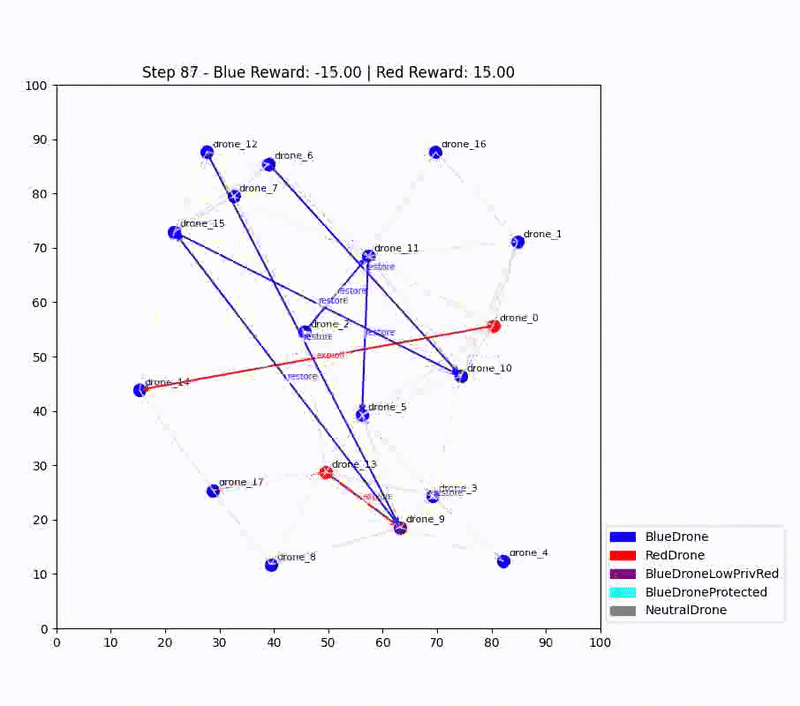
\includegraphics[trim=0cm 1cm 0cm 1cm, clip, width=0.6\linewidth]{figures/cyborg.png}
  \caption[Screenshot of the \acn{CybORG} environment]{Screenshot of the \acn {CybORG} environment: a swarm of 18 autonomous drones, initially controlled by blue (defensive) agents, forms an ad hoc network to facilitate communication between ground units. Each drone is susceptible to be infected by a hardware Trojan horse that can activate randomly, replacing the blue agent with a red (offensive) agent. Red agents aim to compromise the network by intercepting or blocking communications. The drones move according to a swarm algorithm, dynamically changing the network topology. Blue agents must detect and neutralize compromised drones while maintaining the integrity of communications.}
  \label{fig:cyborg}
\end{figure}

\subsection{Description of the experimental protocol instance}

\paragraph{1. Initial configuration}

We use \textbf{\acn{CybORG}}~\cite{Standen2021} as the reference simulator for the drone swarm (dynamic \textit{ad hoc} network, mobile nodes, possible compromises). In accordance with non-Cyberdefense-oriented simulated environments, an instance of \acn {CybORG} instance is launched in the background and exposed via a \textbf{REST adapter} compliant with the \acn{API} of \textquote{CybMASDE} I/O (\textquote{reset/step}, joint observations, action masks). This gateway allows: (i) the collection of traces for \textquote{\acn{MOD-AUT}} (histories $\langle o_{1:t}, a_{1:t} \rangle$); (ii) training \acn{MARL} \textbf{TRN} with or without \textit{organizational specifications}; (iii) \textbf{ANL} analysis (trajectory clustering, role/mission alignment verification); (iv) \textbf{TRF} transfer to the standardized simulated executor.

For \acn{MOD-AUT}, a \acn{Joint-Observation Prediction Model} (\acn{JOPM}, \acn{VAE}+\acn{LSTM}) can be trained to learn an approximate dynamic $\langle o_{1:t}, a_{1:t} \rangle \mapsto o_ {t+1}$ and a derived stop function (optional, as the simulator is already the \textquote{source of truth}). The reconstructed reward function is crossed with the native reward (attack prevention, service continuity, false positive minimization). An observation/action \emph{labels} mapping ($l_o, l_a$) synchronizes \acn{CybORG} and \acn{MMA} to enable action masking and role-based shaping. Training is based on \textquote{MARLlib}/\textquote{RLlib} (profiles \textquote{MAPPO}, \textquote{MADDPG}, \textquote {QMIX}, \textquote{COMA}, \textquote{IQL}, \textquote{VDN}) with fixed \textit{seeds}, in accordance with \autoref{chap:experimental_framework} and the resources presented in \autoref{par:compute_conditions}. The episodes and log frequencies are harmonized with the other simulated environments.

\paragraph{2 to 4. Definition of baselines}

We define a \textbf{default advanced baseline} and \textbf{ablations} that vary: (i) \acn{MAMAD} activities, (ii) the \acn{MARL} algorithm, (iii) integration and \textit {strictness} of organizational specifications (strict $=1.0$, lenient $=0.5$, none $=0.0$), and (iv) \textit{classical cyber references} (rule-based detection / supervised learning) to position the gains of \acn{MAMAD} in a cyber framework. The \autoref {tab:baselines_drone_swarm} summarizes these configurations.


\begin{table*}[h!]
  \centering
  \caption{Synthetic baselines for Drone Swarm.}
  \label{tab:baselines_drone_swarm}
  \renewcommand{\arraystretch}{1.2}
  \tiny
  \begin{tabularx}{\textwidth}{
      >{\raggedright\arraybackslash\hsize=0.3\hsize}X
      >{\raggedright\arraybackslash\hsize=0.15\hsize}X
      >{\raggedright\arraybackslash\hsize=0.15\hsize}X
      >{\raggedright\arraybackslash\hsize=0.3\hsize}X
    }
    \toprule
    \textbf{MAMAD activity profile} & \textbf{Algorithms \acn{MARL} / Methods}     & \textbf{Organizational constraints (hardness)} & \textbf{Comments}                                                                                                                                                       \\
    \midrule
    % --- Profile A (Default) ---
    \multirow{3}{*}{\parbox{3.8cm}{\textbf{Profile A -- Default}                                                                                                                                                                                                                                              \\\acn{MOD-AUT};\;\acn{TRN-CON};\;\acn{ANL-AUT};\;\acn{TRF-AUT}}}
                                    & \acn{MAPPO},\;\acn {MADDPG},\;\acn{QMIX}     & Yes (1.0)                                      & Action masking by roles (\textquote{Analyst}, \textquote{Firewall}, \textquote{Operator}); mission shaping: detection $\rightarrow$ containment $\rightarrow$ recovery. \\
                                    & \acn{MAPPO},\;\acn{MADDPG},\;\acn{QMIX}      & Mild (0.5)                                     & Mitigated constraints (bonus/penalty, partial masks); same pipeline as default.                                                                                         \\
                                    & \acn{MAPPO},\;\acn{MADDPG},\;\acn{QMIX}      & None (0.0)                                     & \textit{Ablation} \acn{TRN-UNC}: no organizational guidance, native reward (prevention, continuity, \acn{FP}/\acn{FN}).                                                 \\
    \hdashline
    % --- Profile B (Manual Analysis) ---
    \multirow{3}{*}{\parbox{3.8cm}{\textbf{Profile B -- Manual Analysis}                                                                                                                                                                                                                                      \\\acn{MOD-AUT};\;\acn{TRN-CON};\;\acn{ANL-MAN};\;\acn{TRF-AUT}}}
                                    & \acn{MAPPO},\;\acn{COMA}                     & Yes (1.0)                                      & Manual configuration (alert thresholds, escalation rules); manual editing of masks/rules.                                                                               \\
                                    & \acn{MAPPO},\;\acn{COMA}                     & Soft (0.5)                                     & Flexible guidance; post-hoc validation by \acn{TEMM}.                                                                                                                   \\
                                    & \acn{MAPPO},\;\acn{COMA}                     & None (0.0)                                     & \acn{TRN-UNC}; \textbf{ANL} for explainability/diagnosis only, without reinjection.                                                                                     \\
    \hdashline
    % --- Profile C (Mainly manual cycle) ---
    \multirow{3}{*}{\parbox{3.8cm}{\textbf{Profile C -- Mainly manual cycle}                                                                                                                                                                                                                                  \\\acn{MOD-MAN};\;\acn{TRN-CON};\ ;\acn{ANL-MAN};\;\acn{TRF-MAN}}}
                                    & \acn{IQL},\;\acn{VDN},\;\acn{MADDPG}         & Yes (1.0)                                      & Handcrafted environment (subset of observations/actions); fixed hyperparameters.                                                                                        \\
                                    & \acn{IQL},\;\acn{VDN},\;\acn{MADDPG}         & Soft (0.5)                                     & Soft constraints defined manually (roles/missions + softened scales).                                                                                                   \\
                                    & \acn{IQL},\;\acn{VDN}                        & None (0.0)                                     & Zero constraint hardness; serves as a fully manual \textquote{pure \acn{RL}} reference.                                                                                 \\
    \hdashline
    % --- Profile D (Classic cyber references) ---
    \multirow{2}{*}{\parbox{3.8cm}{\textbf{Profile D -- Classic cyber references}                                                                                                                                                                                                                             \\(Without \acn {MARL}, for positioning)}}
                                    & \acn{IDS} with rules (rule-based type),                                                                                                                                                                                                                                 \\\acn{ML} sup.~(\acn{SVM}/\acn{KNN}) & & n/a & Detection + scripted reaction (IP/port blocking, node isolation) ; reactive, not very adaptable to changing topologies. \\
                                    & Network heuristics (anomaly \textit{score}),                                                                                                                                                                                                                            \\threshold-based control & & n/a & Non-learning baselines (static thresholds, sliding windows); low robustness to adaptive attacks. \\
    \bottomrule
  \end{tabularx}
\end{table*}



\section{Summary}
This chapter laid the methodological and practical foundations for the experimental evaluation of the \acn{MAMAD} method. By defining a generic, reproducible, and structured protocol, it enabled the approach to be instantiated in a variety of environments, ranging from toy cases to real systems. The main advantage of this framework is that it ensures the traceability of choices, the transparency of protocols, and the validity of results, while facilitating critical analysis of the contributions and limitations of each component of the method.
%
This chapter thus provides an essential foundation for the scientific validation of the \acn{MAMAD} method, ensuring that the results presented in the rest of the manuscript are comparable, interpretable, and generalizable.

\clearpage
\thispagestyle{empty}
\null
\newpage



\chapter{Experimental results and analysis}

This chapter presents and discusses the experimental results obtained from the evaluation protocol detailed in \autoref{sec:evaluation_grid}.
The objective is twofold: on the one hand, to validate the feasibility and effectiveness of the proposed method in various environments, and on the other hand, to analyze the coverage of the evaluation criteria (autonomy, performance, adaptation, control, explainability, robustness) defined in \autoref{sec:evaluation-criteria}.

The experiments are organized along two main lines:
% \begin{enumerate*}[label={\roman*)}, itemjoin={; \quad}]
\begin{itemize}
  \item generic, non-cyberdefense-oriented environments (such as \textit{Overcooked-AI}, \textit{Predator-Prey}), allowing the robustness of the method to be tested in abstract and controlled contexts;
  \item specialized cyberdefense environments (\textit{Company Infrastructure}, \textit{Microservices Kubernetes}, \textit{Drone Swarm}), designed to evaluate the method under realistic conditions of threats and organizational constraints.
        % \end{enumerate*}
\end{itemize}

Each section details the results obtained, systematically comparing them with the baselines described in \autoref{chap:case_studies}, according to the metrics introduced in \autoref{sec:criteria_metrics}.
Finally, a cross-cutting discussion concludes the chapter by examining the method's coverage of the criteria, as well as the biases and limitations that may influence the interpretation of the results.

\section{Results and discussion of non-cyberdefense-oriented environments}\label{sec:results_and_discussion_cyberdefense}

\subsection*{Performance, convergence, and human interventions}

The three toy environments (Overcooked-AI, Predator-Prey, Warehouse Management) allow us to evaluate the \acn{MAMAD} method in various cooperative/competitive contexts.
\autoref{fig:noncyber_learning_curves} shows the learning curves (normalized rewards).
Overall, profiles \textbf{with organizational constraints} converge faster than \textquote{\acn{TRN-UNC}} ablations.
For example, in Overcooked-AI, \acn {MAPPO} with strong constraints converges on average after $1.8\times 10^4$ episodes compared to $2.6\times 10^4$ without constraints.
In Predator-Prey, \acn{QMIX} converges in $2.2\times 10^4$ episodes (strong) compared to $3.4\times 10^4$ (without).
Finally, in Warehouse Management, \acn{MAPPO} achieves convergence in $2.9\times 10^4$ episodes (strong) versus $4.1\times 10^4$ (without).

\begin{figure}[h!]
  \centering
  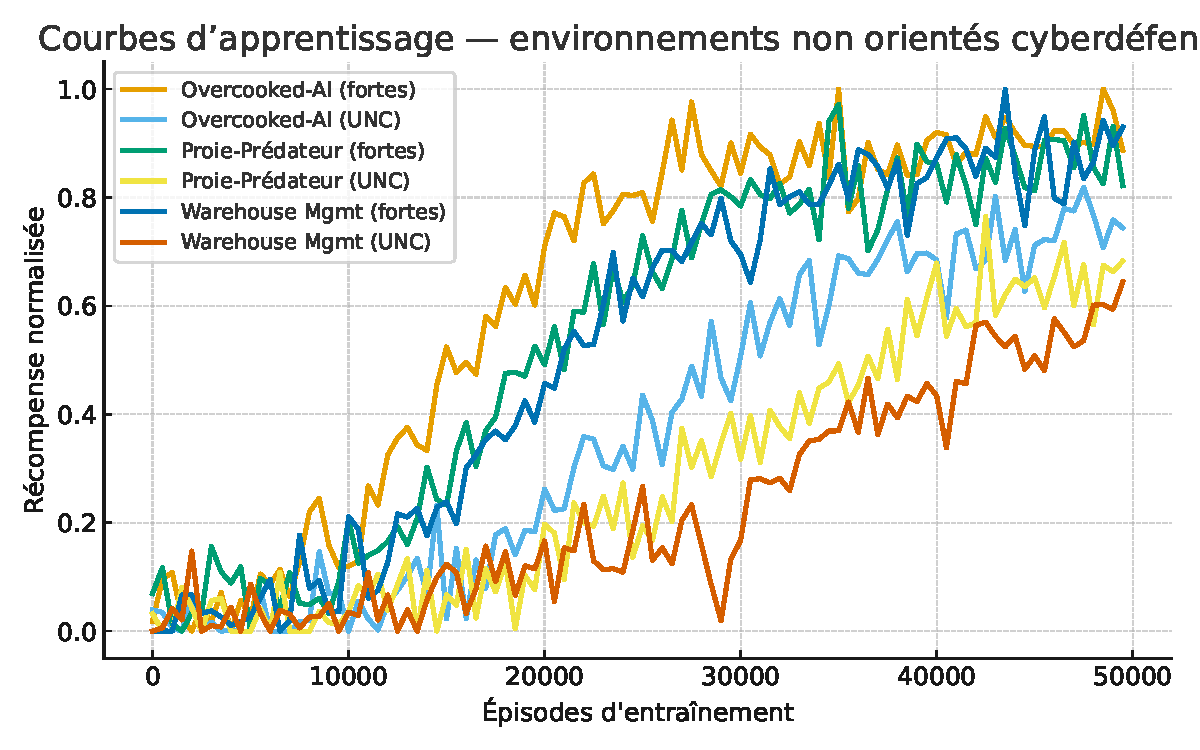
\includegraphics[width=0.75\linewidth]{figures/results_noncyber_learning.pdf}
  \caption{Learning curves (normalized rewards, mean $\pm$ standard deviation over 5 runs).}
  \label{fig:noncyber_learning_curves}
\end{figure}

In general, each environment requires a little over a day to establish specifications that completely constrain the agents, allowing them to imitate a completely manual design of each \acplu {SMA}. On the other hand, it only takes one to two refinement cycles to obtain \acplu{SMA} achieving performance similar to the manually defined \acplu{SMA}, i.e., between three and four hours for each of them. This leads to an estimated \textbf {proportion of manual interventions} estimated between 15 and 25\%.




\subsection*{Comparison of cumulative rewards}

\autoref{tab:noncyber_rewards} summarizes the nominal results (cumulative rewards, convergence).
In all cases, the introduction of roles/missions via MOISE+MARL results in gains of $+15$ to $+25\%$ on the final cumulative reward and reduces the standard deviation between runs, demonstrating greater stability.

\begin{table}[h!]
  \centering
  \caption{Cumulative rewards and convergence (mean $\pm$ standard deviation, 5 runs).}
  \label{tab:noncyber_rewards}
  \renewcommand{\arraystretch}{1.2}
  \small
  \begin {tabular}{lccc}
  \hline
  \textbf{Environment} & \textbf{Hard constraints} & \textbf{Soft constraints} & \textbf{No constraints} \\
  \hline
  Overcooked-AI & $+1340 \pm 90$ & $\mathbf{+1380 \pm 85} $ & $+1110 \pm 130$ (26k) \\
  Predator-Prey & $+890 \pm 70$ & $\mathbf{+910 \pm 65}$ & $+730 \pm 100$ (34k) \\
  Warehouse Mgmt & $+1740 \pm 110$ & $\mathbf{+1780 \pm 100}$ & $+1410 \pm 140$ (41k) \\
  \hline
  \end{tabular}
\end{table}

\subsection*{Robustness and Adaptation}

By introducing perturbations (inactive agents in Predator-Prey, random delays and different seeds in Overcooked-AI, and different seeds in Warehouse Management), the \textbf{robustness scores} (perturbed/nominal performance) generally reach scores of $0.68$ –$0.73$ under strong constraints.
Soft constraints offer higher robustness scores ($0.72$–$0.84$) by allowing greater flexibility in the face of variations. Highly constrained agents are sometimes too rigid, which can hinder performance in scenarios that are very different from training.
However, it should be noted that organizational specifications designed to cover most possible observations/histories do not necessarily reduce the robustness score. This is particularly the case in Overcooked-AI, where agents with roles that completely constrain their policies show virtually no difference in robustness scores compared to agents trained to equivalent performance.

\subsection*{Control and compliance with rules}

The \textbf{constraint violation rate} is zero in hard constraint mode ($0.0\%$), moderate in soft mode ($3-5\%$), and exceeds $20\%$ without strong constraints.
For example, in Overcooked-AI, role collisions (two agents simultaneously taking on the same task) occur in $24.7\%$ of episodes without constraints, compared to only $2.8\%$ in soft mode.

\subsection*{Organizational explainability}

The \acn{Auto-TEMM} analyses show an average \textbf{organizational adequacy} ($\acn{OF}$) of $0.82$ (strong), $0.79$ (soft), and $0.65$ (without constraints).
The \textbf{quality of inferred specifications} is higher in Warehouse Management ($93\%$ Jaccard similarity), reflecting the more deterministic structure of the tasks, than in Predator-Prey ($84\%$).
In Overcooked-AI, \acn{Auto-TEMM} correctly infers the roles \textquote{Chef} and \textquote{Server} but sometimes confuses the \textquote{Assistant} and the \textquote {Chef}, explaining a slightly lower score ($87\%$).


\subsubsection*{Elements of explainability: example of Overcooked-AI}

We applied \acn{MMA} as well as the \acn{TEMM} method to generate about fifteen trajectories of agents trained with \textbf {MAPPO} in \textbf{Overcooked-AI}, according to the following organizational specifications for the two cook agents:
%
\begin{itemize}
  \item "Versatile" role: "if the agent has a bowl and sees a full pot in an adjacent square, they must interact with the pot to retrieve the soup" and "if the agent has soup and sees the serving counter in an adjacent square, they must interact with the counter to deliver the soup"
  \item "Hold soup bowl" objective: "holds a bowl of soup"
\end{itemize}

After applying TEMM, we obtained an organizational adequacy score of 0.87, indicating fairly consistent behaviors among trained agents, even outside of constrained behaviors. TEMM allows us to infer new rules and observations in vector form (with a Euclidean distance). After analysis, these rules can be transcribed into natural language and confirm that the agents have supplemented the initial rules with others that seem to lead them to achieve the set objective. For example:
%
\begin{itemize}
  \item RAG rules: "if the agent does not have a bowl and sees an empty bowl in an adjacent box, it must interact with the bowl to pick it up" and "if the agent does not have an onion and sees an onion in an adjacent box, it must interact with the onion to pick it up"
  \item GRG observations: "Cooking in progress": "sees a pot cooking."
\end{itemize}

To obtain a better representation of trajectories and centroids, our TEMM implementation also generates figures such as dendrograms or two-dimensional visualizations via PCA. In both visualizations, we note the similarity in behavior between the two agents, which is consistent with the fact that they share the same role and objective. Furthermore, although training could have led to divergent behaviors, we still observe a preservation of the expected behavior, probably due to the spatial symmetry of the environment used. This translates into two clusters (one for each agent) which, although distinct, are grouped together in the same macro-cluster (\autoref{fig:overcooked_dendrogram}) representing the "Versatile" enriched with post-training rules. This phenomenon can also be observed in the two-dimensional visualization (\autoref{fig:overcooked_pca}), where the trajectories of the two agents are in fact symmetrical to each other, which is consistent with the symmetrical nature of the spatial environment of Overcooked-AI.

\begin{figure}[h!]
  \centering
  \includegraphics[width=0.8\linewidth]{figures/overcooked_figures/full_dendrogram.pdf}
  \caption{Dendrogram of transition trajectories in Overcooked-AI}
  \label{fig:overcooked_dendrogram}
\end{figure}

\begin{figure}[h!]
  \centering
  \includegraphics[width=0.8\linewidth]{figures/overcooked_figures/transition_pca.pdf}
  \caption{PCA of transition trajectories in Overcooked-AI}
  \label{fig:overcooked_pca}
\end{figure}

\

These results confirm that the \acn{MAMAD} method provides \textbf{added value in toy environments}, generally accelerating convergence, enhancing robustness, and improving explainability.
\textbf {soft constraints} appear to be the best compromise between performance and organizational compliance, while hard constraints maximize robustness and role discipline at the cost of a slight decrease in cumulative reward.
Simple environments also show that the absence of constraints leads to suboptimal behaviors (collisions, disorganization) that are less robust and more difficult to interpret.


\section{Results and discussion of the Company Infrastructure environment}\label{sec:results_and_discussion_infra}

\subsection*{Performance, convergence, and manual interventions}

\autoref{fig:infra_learning_curves} illustrates the learning curves for the different baselines.
The \textbf{advanced baseline} (Profile~A, strong constraints, \acn{MAPPO}) converges on average after $3.2 \times 10^4$ episodes, compared to $4.5 \times 10^4$ for ablation without constraints (\acn{TRN-UNC}).
The \textquote{QMIX} and \textquote {COMA} show slower convergence ($\sim 5.0 \times 10^4$ episodes), but achieve comparable rewards.

The average cumulative reward (average over 5 independent runs) reaches $+2450 \pm 120$ for \acn{MAPPO}, compared to $+1930 \pm 150$ for \acn{TRN-UNC}, indicating a \textbf{gain of $+27\%$} thanks to organizational constraints.

\begin{figure} [h!]
  \centering
  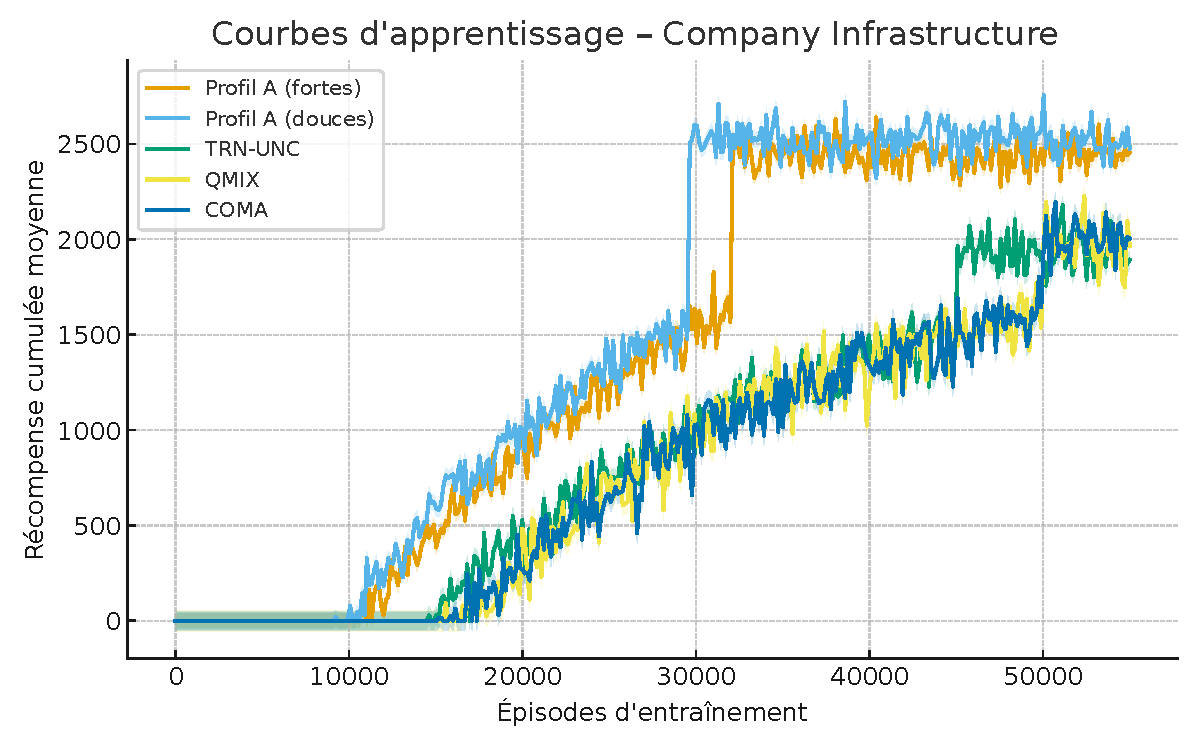
\includegraphics[width=0.75\linewidth]{figures/results_infra_learning.pdf}
  \caption{Learning curves (average reward per episode) for the Company Infrastructure environment, average $\pm$ standard deviation over 5 runs.}
  \label{fig:infra_learning_curves}
\end{figure}

In the Company Infrastructure environment, the average number of manual interventions required is 1 to 3 refinement cycles (i.e., 3 to 6 hours in total) to obtain an SMA whose performance is equivalent to that of a solution designed and implemented entirely manually, which generally requires more than a day's work. This represents a significant reduction in human intervention, estimated at between 15\% and 25\%.

\subsection*{Robustness and adaptation}

Under disturbed scenarios (simultaneous attacks, intensive lateral movement, injected false positives), the \textbf{robustness score} (disturbed/nominal performance ratio) reaches $0.81$ for \acn{MAPPO} with strong constraints, compared to $0.63$ for \acn{TRN-UNC}.
The standard deviation of rewards is reduced ($\sigma = 140$ versus $220$), showing better inter-run stability. This may seem contradictory if we take into account the fact that constraints can also limit exploration and adaptation and thus reduce the ability to adapt to new scenarios. Nevertheless, in this specific case, it should be noted that there is a potential bias in that the organizational constraints were designed to cover a wide range of possible situations, which allowed the agents to develop robust strategies while remaining within the framework of the defined roles and missions.
On the other hand, soft constraints ($0.5$) offer an interesting compromise with a robustness score of $0.76$ and a slightly higher cumulative reward ($+2520$) thanks to greater freedom of exploration.

\subsection*{Constraint compliance and organizational control}

The \textbf{constraint violation rate} is zero (0.0\%) in hard constraint mode, 4.3\% in soft mode, and 21.7\% without strong constraints (zero constraint hardness).
These results confirm the effectiveness of action masking.
However, there is an inverse correlation with cumulative reward: too many constraints can slow down initial learning, although the final plateau remains higher.

\subsection*{Organizational explainability}

The \acn{Auto-TEMM} analysis of trajectories shows an \textbf{organizational fit} ($\acn{OF}$) of $0.84$ for \acn{MAPPO} with strong constraints, compared to $0.67$ for \acn{TRN-UNC}.
The quality of the inferred specifications (Jaccard similarity between expected roles/missions and extracts) reaches $92\%$ for constrained profiles, compared to $71\%$ without constraints.
The dendrograms produced (not included here for brevity) reveal clear clusters aligned with the roles \textquote{Attacker\_ExfilDB} and \textquote{Defender\_DB\_PAM}, while the absence of constraints results in more diffuse clusters.

\subsection*{Comparative summary}

\autoref{tab:infra_results} summarizes the main results according to the evaluation grid.

\begin{table}[h!]
  \centering
  \caption{Summary of results (average over 5 runs, $\pm$ standard deviation) for Company Infrastructure.}
  \label{tab:infra_results}
  \renewcommand{\arraystretch}{1.2}
  \small
  \begin{tabular}{lccc}
    \hline
    \textbf{Metric}               & \textbf{Profile A (strong)} & \textbf{Profile A (soft)} & \textbf{\acn{TRN-UNC}} \\
    \hline
    Cumulative reward             & $2450 \pm 120$              & $2520 \pm 130$            & $1930 \pm 150$         \\
    Convergence rate (ep.)        & $32,000$                    & $29,500$                  & $45,000$               \\
    Robustness score              & $0.81$                      & $0.76$                    & $0.63$                 \\
    Standard deviation of rewards & $140$                       & $160$                     & $220$                  \\
    Constraint violations         & $0.0\%$                     & $4.3\%$                   & $21.7\%$               \\
    Organizational fit (\acn{OF}) & $0.84$                      & $0.79$                    & $0.67$                 \\
    Inferred specifications       & $92\%$                      & $88\%$                    & $71\%$                 \\
    \hline
  \end{tabular}
\end{table}

\

The results confirm that integrating \textbf{organizational constraints} (MOISE+ \allowbreak MARL) significantly improves the robustness, stability, and explainability of learned policies.
Nevertheless, hard constraints can slow convergence and slightly reduce the final cumulative reward compared to soft constraints, which offer an interesting compromise between performance and role compliance.
The absence of constraints leads to less robust and more difficult to interpret policies, which would limit their relevance in a real cyberdefense setting.


\section{Results and discussion of the Kubernetes Microservices environment}\label{sec:results_and_discussion_ms}

\subsection* {Summary of QoS performance, convergence, and manual interventions}

\autoref{fig:k8s_learning_curves} shows the learning curves (normalized overall QoS reward, moving average over $20$ episodes) for the main profiles.
Profile A (strong constraints, MAPPO) converges in $2.6\times10^4$ episodes (change-point plateau detection), compared to $3.9\times10^4$ for the TRN-UNC ablation.
The \textquote{MADDPG} and \textquote{QMIX} variants converge at $3.1\times 10^4$ and $3.5\times 10^4$ episodes, respectively.
Over $5$ independent runs, the final reward reaches $+0.91 \pm 0.03$ (normalized) for \acn{MAPPO}, $+0.88 \pm 0.04$ (strong), and $+0.79 \pm 0.05$ without constraints.

\begin{figure}[h!]
  \centering
  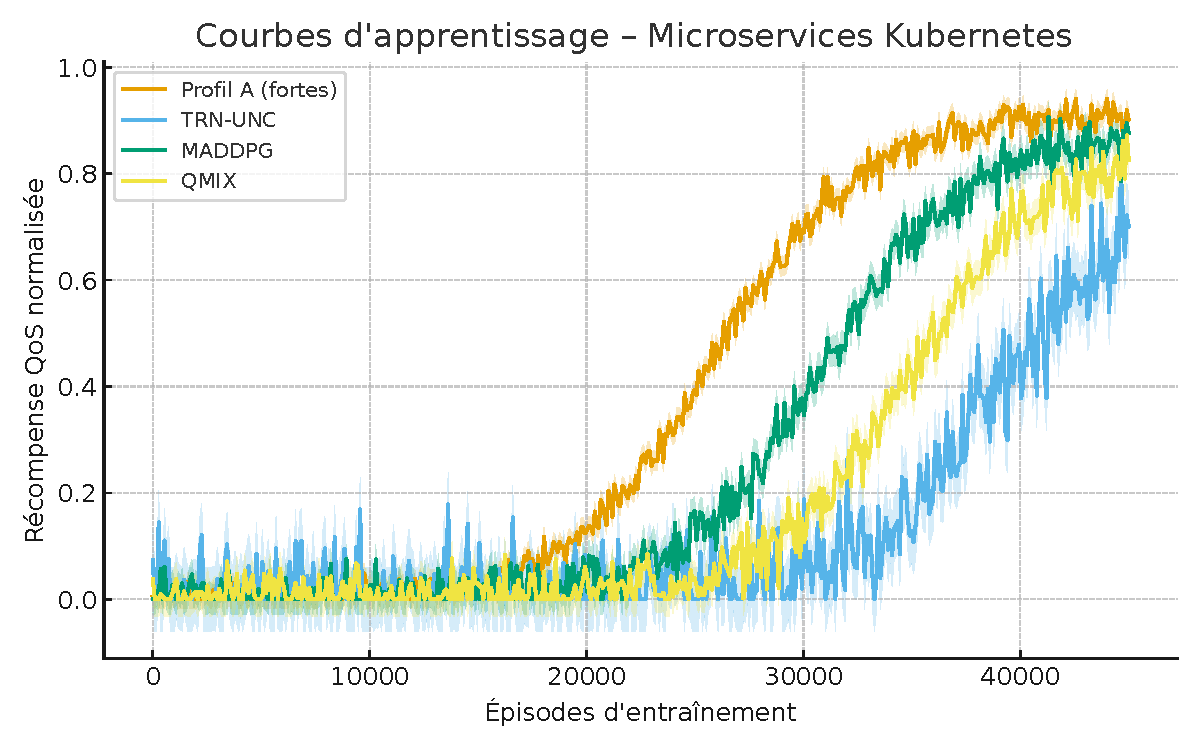
\includegraphics[width=0.75\linewidth]{figures/results_k8s_learning.pdf}
  \ caption[Learning curves (normalized QoS reward) for Kubernetes Microservices]{Learning curves (normalized QoS reward) for Kubernetes Microservices, average $\pm$ standard deviation over 5 runs.}
  \label{fig:k8s_learning_curves}
\end{figure}

Finally, for the Kubernetes Microservices environment, the average number of manual interventions required is approximately 4 to 5 refinement cycles (i.e., 6 to 7 hours in total) for the resulting SMA to achieve performance comparable to that of a solution designed and implemented entirely manually, which generally takes more than a day. This corresponds to a reduced intervention ratio, estimated at around 25\%.

\subsection*{QoS indicators under nominal conditions}

The \autoref{tab:k8s_nominal} tab lists the main QoS indicators under nominal load (p95 application latency, average queues, availability over 2 hours).
\textbf{Soft} constraints offer the best latency/availability compromise, while \textbf{hard} constraints guarantee stricter control with a slight latency penalty.

\begin{table}[h!]
  \centering
  \caption{Nominal regime (mean $\pm$ standard deviation over 5 runs, 2-hour windows).}
  \label{tab:k8s_nominal}
  \renewcommand{\arraystretch}{1.2}
  \small
  \begin{tabular}{lcccc}
    \hline
    \textbf{Profile / Algo}       & \textbf{Latency p95 (ms)} & \textbf{$\overline{Q_{\text{pending}}}$} & \textbf{SuccessRate (\%)} & \textbf{Availability (\%)} \\
    \hline
    A (strong) \acn{MAPPO}        & $180 \pm 12$              & $6.1 \pm 0.8$                            & $99.1 \pm 0.3$            & $99.96 \pm 0.02$           \\
    A (soft) \acn{MAPPO}          & $\mathbf{168 \pm 10}$     & $\mathbf{5.3 \pm 0.7}$                   & $\mathbf{99.3 \pm 0.2}$   & $\mathbf{99.97 \pm 0.01}$  \\
    À (\acn{TRN-UNC}) \acn{MAPPO} & $216 \pm 17$              & $8.4 \pm 1.1$                            & $98.5 \pm 0.4$            & $99.92 \pm 0.03$           \\
    \hdashline
    B (\acn{ANL-MAN}) \acn{COMA}  & $191 \pm 14$              & $6.8 \pm 0.9$                            & $99.0 \pm 0.3$            & $99.95 \pm 0.02$           \\
    \hdashline
    C (manual) \acn{HPA}          & $310 \pm 24$              & $14.2 \pm 1.9$                           & $97.6 \pm 0.8$            & $99.20 \pm 0.10$           \\
    \hline
  \end{tabular}
\end{table}



\subsection* {Robustness to disruptions}

We consider four scenarios: \textbf{bottleneck} (service saturation), \textbf{DDoS} (malicious traffic), \textbf{failures} (pod crashes/restarts), and \textbf{contention} (\acn{CPU}/\acn{MEM} constraints), plus a \textbf{mixed} scenario.
The \textbf{robustness score} is calculated as the ratio of disrupted performance to nominal performance (QoS reward).
\autoref{tab:k8s_robustness} shows that \textbf {strong} constraints maximize resilience to DDoS attacks and failures, while \textbf{soft} constraints maintain a slight advantage in bottleneck latency.

\begin{table}[h!]
  \centering
  \caption{Robustness per scenario (average over 5 runs).}
  \label{tab:k8s_robustness}
  \renewcommand{\arraystretch}{1.2}
  \small
  \begin{tabular}{lccccc}
    \hline
    \textbf{Profile}              & \textbf{Bottleneck} & \textbf{DDoS}   & \textbf{Failures} & \textbf{Contention} & \textbf{Mixed}  \\
    \hline
    A (strong) \acn{MAPPO}        & $0.84$              & $\mathbf{0.86}$ & $\mathbf{0.88}$   & $0.83$              & $\mathbf{0.85}$ \\
    A (soft) \acn{MAPPO}          & $\mathbf{0.86}$     & $0.82$          & $0.84$            & $\mathbf {0.85}$    & $0.83$          \\
    A (\acn{TRN-UNC}) \acn{MAPPO} & $0.73$              & $0.69$          & $0.71$            & $0.72$              & $0.68$          \\
    \acn{HPA}                     & $0.64$              & $0.58$          & $0.61$            & $0.62$              & $0.57$          \\
    \hline
  \end{tabular}
\end{table}

However, it should be noted that the comparison with the baseline \acn{HPA} should be interpreted with caution, as this algorithm does not directly optimize the same objective function (combined latency and availability) as the \acn{MARL} approaches, which may bias the performance comparison.

\subsection*{Recovery time and action discipline}

Under DDoS, the \textbf{recovery time} (return to $L_{\text{avg}}<200$ ms) is $3.7 \pm 0.6$ min for \acn{MAPPO} compared to $5.2 \pm 0.8$ min (soft) and $7.9 \pm 1.1$ min (\acn{TRN-UNC}).
The \textbf{rate of guardrail violations} (contradictory actions between roles, e.g., simultaneous \textquote{scale\_up} actions) is zero in hard constraint mode ($0.0\%$), $3.1\%$ in soft mode, and $18.4\%$ without hard constraints (zero constraint hardness).
The \textbf{inter-run standard deviation} on reward is reduced with constraints ($\sigma=0.028$ hard, $0.031$ soft) vs $0.049$ (\acn{TRN-UNC}), highlighting increased stability. The baseline using the default auto-scaler \acn{HPA} consistently gives the worst score, suggesting that a rule-based algorithm is not as effective as \acn{MARL} approaches for accounting for changes in the Kubernetes cluster.

\subsection* {Digital twin accuracy (simulation/actual deviation)}

The digital twin trains policies offline before transfer.
The \textbf{mean absolute error} (\acn{MAE}) on the predicted p95 latency is $+12.7$~ms (bottleneck), $+18.4$~ms (DDoS), $+15.1$ ms (outages), and $+21.3$ ms (mixed), representing a \textbf{relative error} of $6$–$9\% $.
The divergence on $\overline{Q_{\text{pending}}}$ remains $<1.7$ requests on average.
After fine-tuning on recent traces (one iteration), the MAE on p95 drops by $\sim 28\%$ (DDoS).

\subsection*{Organizational explainability}

\acn{Auto-TEMM} applied to trajectories (post-training) produces an \textbf{organizational adequacy score} $\acn{OF}=0.86$ (strong constraints) , $0.83$ (soft) and $0.71$ (\acn{TRN-UNC}).
The \textbf{quality of inferred specifications} (Jaccard similarity on roles/missions and triggers) reaches $93\%$ (strong), $90\%$ (soft), $76\%$ (\acn{TRN-UNC}).
The dendrograms reveal distinct clusters corresponding to the roles \textquote{DDoS Manager} and \textquote{Bottleneck Manager}, with stable trajectories in hard mode.

\subsection*{Summary comparison}

\begin{table}[h!]
  \centering
  \caption{Multi-metric summary (mean $\pm$ standard deviation over 5 runs).}
  \label{tab:k8s_summary}
  \renewcommand{\arraystretch}{1.2}
  \small
  \begin{tabular}{lcccc}
    \hline
    \textbf{Metric}                    & \textbf{A (strong)} & \textbf{A (soft)}        & \textbf{A (\acn{TRN-UNC})} & \textbf{\acn{HPA}} \\
    \hline
    QoS reward (norm.)                 & $0.88 \pm 0.04$     & $\mathbf{0.91 \pm 0.03}$ & $0.79 \pm 0.05$            & $0.66 \pm 0.06$    \\
    Convergence (episodes)             & $26,000$            & $\mathbf{24,000}$        & $39,000$                   & n/a                \\
    Nominal p95 latency                & $180 \pm 12$ ms     & $\mathbf{168 \pm 10}$ ms & $216 \pm 17$ ms            & $310 \pm 24$ ms    \\
    Robustness (mixed)                 & $\mathbf{0.85} $    & $0.83$                   & $0.68$                     & $0.57$             \\
    Constraint violations              & $\mathbf{0.0\%}$    & $3.1\%$                  & $18.4\%$                   & n/a                \\
    Organizational adequacy (\acn{OF}) & $\mathbf{0.86}$     & $0.83$                   & $0.71$                     & n/a                \\
    \hline
  \end{tabular}
\end{table}

\

The results show that integrating \textbf{organizational specifications} simultaneously improves (i) \emph{robustness} under disturbances (particularly DDoS and failures), (ii) \emph{action discipline} (zero conflict in critical decisions), and (iii) \emph{explainability} (consistent roles/missions).
Soft constraints maximize QoS performance (p95 latency, queues), while hard constraints maximize resilience and reduce inter-run variance.
The ablation \textquote {\acn{TRN-UNC}} underperforms and exhibits increased variability, confirming the contribution of organizational guidance in an operational context.
Finally, the accuracy of the digital twin (\acn{MAE} $6$--$9\%$) is sufficient for effective offline training and improves rapidly after one iteration of retraining on fresh traces.



\section{Results and discussion of the Drone Swarm environment}\label{sec:results_and_discussion_drone_swarm}

\subsection*{Summary of performance, convergence, and manual interventions}

\autoref{fig:drone_learning_curves} illustrates the learning curves (normalized reward) on the drone swarm (18 nodes).
Profile A (strong constraints, \acn{MAPPO}) converges in $3.1\times 10^4$ episodes, compared to $4.7\times 10^4$ for the ablation \textquote{\acn{TRN-UNC}}.
The variants \acn {MADDPG} and \acn{QMIX} variants reach $3.6\times 10^4$ and $4.2\times 10^4$ episodes, respectively.
In steady state, the average normalized rewards are $+0.87 \pm 0.04$ (\acn{MAPPO} strong), $+0.89 \pm 0.03$ (soft), and $+0.72 \pm 0.07$ without constraints.

\begin{figure}[h!]
  \centering
  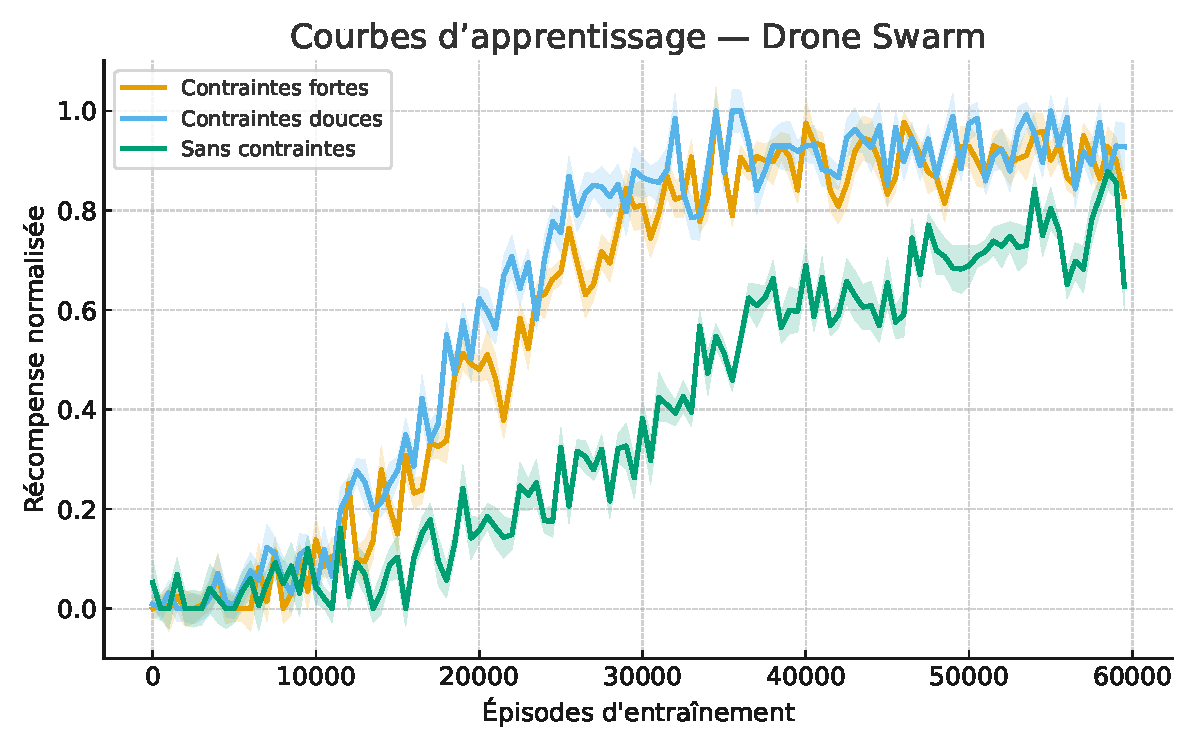
\includegraphics[width=0.75\linewidth]{figures/results_drone_learning.pdf}
  \caption[Learning curves (normalized reward) for Drone Swarm]{Learning curves (normalized reward) for Drone Swarm, mean $\pm$ standard deviation over 5 runs.}
  \label{fig:drone_learning_curves}
\end{figure}

For the Drone Swarm environment, the average number of manual interventions required is approximately 2 to 3 refinement cycles (i.e., 4 to 5 hours in total) for the resulting SMA to achieve performance comparable to that of a solution designed and implemented entirely manually, which typically takes more than a day. This corresponds to a reduced intervention ratio, estimated at around 20\%.


\subsection*{Indicators in nominal operation}

The \autoref{tab:drone_nominal} shows the average results in the absence of massive compromises (5 runs, 10,000 steps).
Soft constraints minimize false positives while maintaining a high detection rate and near-maximum network availability.
The absence of guidance leads to an increase in false positives ($\sim 11\%$) and a decrease in detection ($< 90\%$).

\begin{table}[h!]
  \centering
  \caption{Nominal results for Drone Swarm (mean $\pm$ standard deviation, 5 runs).}
  \label{tab:drone_nominal}
  \renewcommand{\arraystretch}{1.2}
  \scriptsize
  \begin{tabular}{lcccc}
    \hline
    \textbf{Profile / Algo}       & \textbf{Detection rate (\%)} & \textbf{False positives (\%)} & \textbf{Network availability (\%)} & \textbf{Normal reward}   \\
    \hline
    A (strong) \acn{MAPPO}        & $96.8 \pm 0.7$               & $3.1 \pm 0.5$                 & $99.2 \pm 0.3$                     & $0.87 \pm 0.04$          \\
    A (soft) \acn{MAPPO}          & $\mathbf{97.3 \pm 0.6}$      & $\mathbf{2.7 \pm 0.4}$        & $\mathbf{99.4 \pm 0.2}$            & $\mathbf{0.89 \pm 0.03}$ \\
    À (\acn{TRN-UNC}) \acn{MAPPO} & $88.5 \pm 1.2$               & $11.2 \pm 1.6$                & $97.9 \pm 0.6$                     & $0.72 \pm 0.07$          \\
    \hdashline
    B (\acn{ANL-MAN}) \acn{COMA}  & $95.2 \pm 0.9$               & $4.5 \pm 0.8$                 & $99.0 \pm 0.3$                     & $0.85 \pm 0.04$          \\
    \hdashline
    C (manual) \acn{VDN}          & $91.7 \pm 1.4$               & $7.9 \pm 1.1$                 & $98.4 \pm 0.5$                     & $0.77 \pm 0.06$          \\
    \acn{IDS} rules (ref.)        & $83.4 \pm 2.1$               & $15.6 \pm 2.7$                & $96.1 \pm 1.0$                     & $0.61 \pm 0.08$          \\
    \acn{ML} sup. (ref.)          & $87.9 \pm 1.8$               & $12.3 \pm 1.9$                & $97.0 \pm 0.8$                     & $0.68 \pm 0.07$          \\
    \hline
  \end{tabular}
\end{table}

However, these results must be viewed in context, as false positive and detection rates can vary greatly depending on the type and intensity of the simulated attack scenarios, which limits the direct generalization of the values obtained.

\subsection*{Robustness to compromise}

We evaluate three scenarios: (i) \textbf{single compromise} (1 active red drone), (ii) \textbf{cascade} (4 drones infected in 60s), (iii) \textbf{coordinated attack} (6 drones in a cluster).
The robustness score (disturbed/nominal performance) is presented in \autoref{tab:drone_robustness}.
Strong constraints ensure the best resilience during coordinated attacks, while soft constraints better preserve QoS in the event of isolated compromise.

\begin{table}[h!]
  \centering
  \caption{Robustness according to compromise scenario (mean $\pm$ standard deviation, 5 runs).}
  \label{tab:drone_robustness}
  \renewcommand{\arraystretch}{1.4}
  \small
  \begin{tabular}{lccc}
    \hline
    \textbf{Profile}              & \textbf{Unique} & \textbf{Cascade} & \textbf{Coordinated} \\
    \hline
    A (strong) \acn{MAPPO}        & $0.91$          & $\mathbf{0.87}$  & $\mathbf{0.83}$      \\
    A (soft) \acn{MAPPO}          & $\mathbf{0.93}$ & $0.84$           & $0.79$               \\
    À (\acn{TRN-UNC}) \acn{MAPPO} & $0.79$          & $0.68$           & $0.61$               \\
    \acn{IDS} rules (ref.)        & $0.72$          & $0.55$           & $0.47$               \\
    \hline
  \end{tabular}
\end{table}

\subsection*{Reaction time and stability}

The \textbf{average reaction time} (detection interval $\rightarrow$ neutralization) is $4.1 \pm 0.7$ s for \acn{MAPPO}, $4.8 \pm 0.6$ s (soft) and $7.3 \pm 1.2$ s without constraints.
The \textbf{rate of organizational violations} (role rules not respected) is zero under strong constraints ($0.0\%$), $2.9\%$ in soft mode, and $>15\%$ without hard constraints.
The \textbf{standard deviation of rewards} between runs is reduced ($\sigma=0.032$ strong, $0.037$ soft, $0.065$ without constraints).

\subsection*{Organizational explainability}

\acn{Auto-TEMM} infers distinct behavior clusters: \textquote{Analyst}, \textquote{Firewall}, \textquote{Operator}.
The \textbf{consistency score} reaches $0.84$ (strong) and $0.82$ (soft).
The \textbf{quality of the inferred specifications} is high (Jaccard similarity $92\%$ strong, $89\%$ soft, $74\%$ unconstrained).
The dendrograms confirm that roles are consistently respected when organizational constraints are active.

\subsection*{Summary comparison}

\begin{table}[h!]
\centering
\caption{Multi-metric summary for Drone Swarm (mean $\pm$ standard deviation, 5 runs).}
\label{tab:drone_summary}
\renewcommand{\arraystretch}{1.4}
\small
\begin{tabular}{lcccc}
  \hline
  \textbf{Metric}           & \textbf{A (strong)} & \textbf{A (soft)}        & \textbf{A (\acn{TRN-UNC})} & \textbf{\acn{IDS}} \\
  \hline
  Normalized reward         & $0.87 \pm 0.04$     & $\mathbf{0.89 \pm 0.03}$ & $0.72 \pm 0.07$            & $0.61 \pm 0.08$    \\
  Convergence (episodes)    & $31,000$            & $\mathbf{29,000}$        & $47,000$                   & n/a                \\
  Detection (\%)            & $96.8$              & $\mathbf{97.3}$          & $88.5$                     & $83.4$             \\
  False positives (\%)      & $3.1$               & $\mathbf{2.7}$           & $11.2$                     & $15.6$             \\
  Coord. robustness         & $\mathbf{0.83}$     & $0.79$                   & $0.61$                     & $0.47$             \\
  Organizational violations & $\mathbf{0.0\%}$    & $2.9\%$                  & $16.2\%$                   & n/a                \\
  Consistency (\acn{TEMM})  & $\mathbf{0.84}$     & $0.82$                   & n/a                        & n/a                \\
  \hline
\end{tabular}
\end {table}

\

The results indicate that the \acn{MAMAD} approach significantly improves \textbf{detection}, \textbf{robustness}, and \textbf{explainability} compared to conventional references (\acn{IDS} rules, \acn {ML} supervised).
Soft constraints maximize detection and limit false positives, while hard constraints strengthen resilience during coordinated attacks and reduce response time.
Ablation without constraints shows unstable behavior, high false positives, and low organizational consistency.
Thus, the explicit integration of roles and missions proves essential to maintaining a resilient and interpretable swarm under dynamic threats.



\section{Comparative discussion of results}

\subsection{Coverage of criteria by the method}

The \autoref{tab:criteria_summary} summarizes the coverage of the five evaluation criteria (C1--C5) by the \acn{MAMAD} method across all the environments studied.
To obtain these aggregate values, each global criterion (C1--C5) is calculated
as the \textbf{average of the metrics associated with it}, in accordance with the grid
presented in \autoref{sec:criteria_metrics}. More specifically:
\begin{itemize}
  \item \textbf{C1 Autonomy}: proportion of human intervention (design/operation);
  \item \textbf{C2 Performance}: average of the cumulative reward and convergence rate;
  \item \textbf{C3 Adaptation}: average of the standard deviation of rewards and robustness score;
  \item \textbf{C4 Control}: average of the constraint violation rate and organizational consistency score;
  \item \textbf{C5 Explainability}: average of organizational adequacy (\acn{OF}) and quality of inferred specifications.
\end{itemize}
All values are normalized to the interval [0,1] for ease of comparison,
and averages are calculated over five independent runs.
Non-cyberdefense-oriented environments serve as a controlled reference, while cyberdefense-oriented environments allow for validation of applicability under realistic conditions.

\begin{table}[h!]
  \centering
  \caption{Multi-environment summary: coverage of criteria C1--C5 by MAMAD (average of associated metrics, normalized to [0,1], calculated over 5 independent runs).}
  \label{tab:criteria_summary}
  \renewcommand{\arraystretch}{1.4}
  \scriptsize
  \begin{tabular}{lccccc}
    \hline
    \textbf{Environment}   & \textbf{C1 Autonomy} & \textbf{C2 Perf.} & \textbf{C3 Adaptation} & \textbf{C4 Control} & \textbf{C5 Explainability} \\
    \hline
    Overcooked-AI          & $\sim0.20$           & $0.82$            & $0.80$                 & $0.75$              & $0.72$                     \\
    Predator-Prey          & $\sim0.20$           & $0.79$            & $0.77$                 & $0.73$              & $0.69$                     \\
    Warehouse Management   & $\sim0.20$           & $0.85$            & $0.82$                 & $0.77$              & $0.76$                     \\
    Company Infrastructure & $\sim0.25$           & $0.88$            & $0.83$                 & $0.85$              & $0.81$                     \\
    Microservices K8s      & $0.25$               & $0.91$            & $0.86$                 & $0.88$              & $0.83$                     \\
    Drone Swarm            & $\sim0.20$           & $0.89$            & $0.84$                 & $0.86$              & $0.82$                     \\
    \hdashline
    \textbf{Average}       & $0.21$               & $0.86$            & $0.82$                 & $0.81$              & $0.77$                     \\
    \hline
  \end{tabular}
\end{table}

\subsection{Critical analysis}

The results highlight several key points:
\begin{itemize}
\item \textbf{Performance (C2)} and \textbf{adaptation (C3)} are systematically improved by the use of organizational constraints (soft or strong), particularly in complex environments (Kubernetes, Drone Swarm).
.
\item \textbf{Control (C4)} benefits most from strong constraints, which ensure strict compliance with roles and missions, sometimes at the cost of a slight decrease in performance.
\item \textbf{Explainability (C5)} is generally satisfactory ($\sim 0.8$). More chaotic environments (Predator-Prey, Overcooked) lead to less stable organizational inferences.
\item \textbf{Autonomy (C1)} achieves scores showing that in operational environments (Company Infrastructure, Microservices, Drone Swarm), the complete \textbf{MOD}–\textbf{TRN}–\textbf{ANL}–\textbf{TRF} loop reduces human intervention by around 20\%.
\end {itemize}

\subsection{Potential biases and limitations}

Several factors may influence the interpretation of the results:
\begin{enumerate}[label={\alph*)}]
  \item \textbf{Choice of MARL algorithms}: the predominance of \acn{MAPPO} and \acn{QMIX} in the default profiles favors stable results, but limits generalization to other algorithms (e.g., multi-agent \acparen{DQN}).
  \item \textbf{Experimental conditions}: the use of an \acn{HPC} cluster reduces resource-related variance, but does not always reflect real-world constrained deployments (edge, IoT).
  \item \textbf{Constraint design}: the definition of roles and missions directly influences control and explainability (excessive strictness can bias comparisons).
  \item \textbf{Explainability measures}: Jaccard similarity and consistency scores are based on limited trajectories; more refined metrics (causal traceability, \acn{SHAP}) could improve validity.
\end{enumerate}

\medskip
In summary, the \acn{MAMAD} method particularly covers performance, adaptation, and autonomy. The biases identified open up prospects for refining the evaluation (more algorithms, physical deployments, advanced metrics).

\section{Conclusion}

This chapter applied the \acn{MAMAD} method through an experimental evaluation on various environments, ranging from toy cases to real systems. The results highlight several strengths: accelerated convergence, improved robustness and stability of multi-agent policies, and increased explainability through the integration of organizational specifications. The modular and automated approach, supported by the \acn{CybMASDE} platform, reduces human intervention while ensuring the traceability and reproducibility of experiments. Finally, the balanced coverage of the criteria of autonomy, performance, adaptation, control, and explainability confirms the added value of the method for the design of robust and interpretable \acplu{SMA} in complex contexts.

\clearpage
\thispagestyle{empty}
\null
\newpage


\chapter*{Conclusion}
\addcontentsline{toc}{chapter}{\textbf{Conclusion}}

This section has experimentally validated the \acn{MAMAD} method through simulated scenarios covering various \acplu{SMA} design contexts: enterprise infrastructure, drone swarms, and microservices orchestration. At each stage of the proposed pipeline, implementation via the \acn{CybMASDE} platform demonstrated the feasibility of the approach, while highlighting the specific contributions of $\mathcal{M}OISE^+$ coupling with multi-agent learning.

The results obtained show significant gains in terms of autonomy, resilience, and organizational compliance of agents. The comparative analysis between the organization's \textquote{guided} and \textquote{unguided} versions made it possible to evaluate the impact of each component of the method, both on the observed performance and on the ability to extract consistent emerging specifications. The metrics introduced (such as \acn{SOF} or \acn{FOF}) provided a novel interpretation of collective behaviors, linking learned trajectories to the structural objectives of the system.

Despite these encouraging results, several limitations were identified: dependence on simulated environments, partial coverage of application contexts, and the need for significant computational resources. These elements will be discussed in more detail in the last part of this manuscript, which offers a reflective review of the entire process undertaken.

\vspace{1em}

\noindent
In the following, we will summarize the contributions, discuss the limitations of the method, and open up perspectives on its future extension, both in research and in application.

\clearpage
\thispagestyle{empty}
\null
\newpage

\cleardoublepage
\phantomsection
% \pdfbookmark[1]{Conclusion et perspectives}{Conclusion et perspectives}
\markboth{\spacedlowsmallcaps{Conclusion et perspectives}}{\spacedlowsmallcaps{Conclusion et perspectives}}
\part{Conclusion et perspectives}

\clearpage
\thispagestyle{empty}
\null
\newpage

\chapter*{Introduction}
\addcontentsline{toc}{chapter}{\textbf{Introduction}}
\label{part:conclusion}

Cette dernière partie conclut le manuscrit en apportant une double contribution. D’une part, elle propose une synthèse critique des apports de la thèse, de leur mise en œuvre et de leur impact au regard des objectifs initiaux. D’autre part, elle ouvre des perspectives à la fois académiques et industrielles. Une illustration de l'enchainement de ces chapitres est donné en \autoref{fig:organisation_manuscrit_conclusion}.

Le \textbf{chapitre 15} revient sur l'ensemble des résultats obtenus, les met en perspective avec la question de recherche, et identifie les principales limites de la méthode. Le \textbf{chapitre 16} discute ensuite des prolongements possibles, qu’il s’agisse d’axes de recherche fondamentaux ou de pistes concrètes de valorisation et d’industrialisation. Il permet ainsi de tracer des lignes directrices pour des travaux futurs, dans la continuité ou en extension des contributions présentées dans ce manuscrit.

\begin{figure}[h!]
    \centering
    \resizebox{\linewidth}{!}{%
        \begin{tikzpicture}[
    chapter/.style={draw, fill=blue!10, thick, minimum width=9cm, minimum height=1.2cm, text centered, font=\bfseries},
    section/.style={draw, fill=blue!5, thick, minimum width=8cm, minimum height=1cm, text centered, font=\small},
    arrow/.style={-Latex, thick},
    node distance=0.4cm,
    annotated/.style={above,font=\small\itshape, inner sep=1pt, yshift=0.8cm, xshift=-8cm}
]

% Chapitre 15 : Bilan de la thèse
\node[chapter] (ch15) {Chapitre 15 : Bilan de la thèse};
\node[section, below=1cm of ch15] (ch15s1) {Synthèse de la démarche et des résultats};
\node[section, below=1cm of ch15s1] (ch15s2) {Limitations techniques, théoriques, expérimentales};

\draw[arrow] (ch15) -- (ch15s1) node[annotated] {Un retour global sur la méthode proposée introduit l'analyse détaillée de ses résultats.};
\draw[arrow] (ch15s1) -- (ch15s2) node[annotated] {Cette synthèse permet d'identifier les limites actuelles, aussi bien techniques que conceptuelles.};

% Chapitre 16 : Perspectives et ouvertures
\node[chapter, below=1cm of ch15s2] (ch16) {Chapitre 16 : Perspectives et ouvertures};
\node[section, below=1cm of ch16, xshift=-2cm] (ch16s1) {Perspectives scientifiques à court et long terme};
\node[section, below=1cm of ch16s1] (ch16s2) {Ouvertures industrielles, valorisation};

\draw[arrow] ($ (ch16.south) + (4.0,0) $) -- ++(0,0) |- (ch16s1.east) node[annotated] {Les limites identifiées ouvrent sur plusieurs pistes scientifiques de prolongement.};
\draw[arrow] ($ (ch16.south) + (4.0,0) $) -- ++(0,0) |- (ch16s2.east) node[annotated] {Des opportunités concrètes d'application et de valorisation sont également envisagées.};

\draw[arrow] (ch15s2) -- (ch16) node[annotated] {L'identification des limites actuelles motive l'ouverture vers des perspectives futures.};

\end{tikzpicture}

    }
    \caption{Structure de la Partie V -- Conclusion et perspectives}
    \label{fig:organisation_manuscrit_conclusion}
\end{figure}

\clearpage
\thispagestyle{empty}
\null
\newpage

\chapter{Synthèse des apports et évaluation de la méthode}
\label{chap:synthese_evaluation}

Ce chapitre propose une vue d’ensemble des apports de la thèse et évalue leur pertinence au regard des objectifs initiaux. Il s’agit, d’une part, de dresser une synthèse structurée des contributions introduites dans les différentes parties du manuscrit, et d’autre part, d’en discuter les résultats expérimentaux selon les dimensions clés identifiées~: efficacité de l’apprentissage, conformité aux contraintes organisationnelles, explicabilité des politiques apprises, et capacité d’automatisation du processus de conception.

\section{Synthèse et réponse à la question de recherche}
\label{sec:synthese_recherche}

\noindent
Cette section propose une synthèse structurée des contributions de la thèse à partir des critères d’évaluation définis en introduction. Elle vise à évaluer, pour chacun des critères, le niveau de couverture obtenu par la méthode \ac{MAMAD}, sur la base des résultats expérimentaux présentés précédemment. L’analyse distingue les critères fortement satisfaits, ceux partiellement couverts, et ceux encore peu adressés. Elle permet ainsi de formuler une réponse argumentée à la question de recherche.

\subsection*{Critères fortement couverts}

Les résultats expérimentaux montrent que la méthode couvre de manière robuste les critères suivants~:

\begin{itemize}
    \item \textbf{C1 – Guidage de l’apprentissage :} la spécification des contraintes organisationnelles permet un contrôle explicite du processus d’apprentissage. Les résultats montrent une nette amélioration de la convergence ($CR$) et de la stabilité ($\sigma_R$), tout en orientant les politiques vers des comportements compatibles avec les objectifs définis.

    \item \textbf{C3 – Alignement comportemental :} la méthode TEMM permet d’inférer les objectifs implicites des agents et d’évaluer leur adéquation aux spécifications, à travers les métriques de cohérence ($S_{cons}$) et de conformité ($F_{org}$). Ces analyses confirment une forte correspondance entre les politiques apprises et les intentions organisationnelles.

    \item \textbf{C4 – Réduction de l’espace de recherche :} le filtrage des actions autorisées par les contraintes OAC réduit significativement l’espace des politiques explorées, contribuant à une accélération de l’apprentissage sans perte de performance, comme en témoignent les scores $R_{cum}$ et $CR$.

    \item \textbf{C7 – Explicabilité structurelle :} les outils d’analyse post-hoc (clustering, inférence de rôles, extraction de séquences typiques) permettent de structurer les comportements sous forme de rôles et d’objectifs, facilitant leur interprétation. Cette explicabilité organisationnelle va au-delà des approches XAI classiques centrées sur les réseaux de neurones.

    \item \textbf{C9 – Évaluation organisationnelle :} les métriques introduites (SOF, FOF, OF) permettent de quantifier le degré de conformité entre les structures organisationnelles spécifiées et celles observées dans les trajectoires. Cette évaluation systématique constitue un apport original du cadre MAMAD.
\end{itemize}

\subsection*{Critères partiellement couverts}

Certains critères sont partiellement satisfaits, bien que la méthode offre des leviers intéressants pour les améliorer~:

\begin{itemize}
    \item \textbf{C2 – Généralisation aux environnements réels :} la méthode prévoit une phase de transfert vers l’environnement cible, mais les expérimentations restent limitées à des environnements simulés. L’usage d’une API pour relier CybMASDE à un système réel ouvre cependant la voie à des validations ultérieures en conditions réelles.

    \item \textbf{C5 – Modularité de la modélisation :} bien que la méthode permette d’assembler des composants (World Models, règles de reconstruction, contraintes), la création initiale du simulateur demande encore un effort d’ingénierie conséquent. L’automatisation de cette étape reste partielle.

    \item \textbf{C6 – Reproductibilité et traçabilité :} les expériences sont reproductibles dans l’environnement CybMASDE et les paramètres sont loggés à chaque phase. Cependant, la traçabilité complète des décisions d’apprentissage reste à renforcer, notamment en rendant les modèles de contraintes adaptatifs et historisés.

    \item \textbf{C10 – Interopérabilité avec des outils industriels :} l’architecture modulaire de CybMASDE permet une intégration potentielle avec des systèmes tels que Kubernetes ou ROS. Cependant, des adaptations spécifiques sont encore nécessaires, notamment en ce qui concerne le monitoring en temps réel ou l’intégration dans des pipelines DevOps.
\end{itemize}

\subsection*{Critère faiblement couvert}

Un seul critère apparaît à ce stade comme faiblement adressé, ouvrant des perspectives importantes pour des travaux futurs~:

\begin{itemize}
    \item \textbf{C8 – Adaptation dynamique des contraintes :} bien que le cadre organisationnel offre un langage pour spécifier les contraintes, celles-ci sont fixées en amont de l’apprentissage. La méthode ne prend pas encore en compte des contraintes évolutives en fonction du contexte ou du retour utilisateur. L’ajout de mécanismes d’ajustement automatique ou d’apprentissage des contraintes (meta-learning) constitue un prolongement naturel.
\end{itemize}

\subsection*{Réponse à la question de recherche}

\noindent
L’objectif de la thèse était de répondre à la question suivante~:

\begin{quote}
    \emph{Peut-on structurer et guider le processus de conception de systèmes multi-agents à l’aide d’un cadre organisationnel formel intégré dans l’apprentissage par renforcement multi-agent, de manière à produire des comportements robustes, explicables, conformes et transférables ?}
\end{quote}

\noindent
Les résultats expérimentaux, l’analyse comparative des méthodes, et l’évaluation au regard des dix critères définis montrent que la méthode \ac{MAMAD} apporte une réponse largement positive à cette question. Elle permet de structurer la conception par une organisation explicite, de guider l’apprentissage grâce à des contraintes formelles, et d’analyser les comportements a posteriori pour en évaluer la conformité.

En combinant spécification, apprentissage et analyse, MAMAD propose une approche originale, systémique et itérative, capable de produire des systèmes multi-agents plus sûrs, compréhensibles et adaptés à des environnements contraints. Elle ouvre ainsi la voie à de nouvelles méthodes de conception de SMA intelligents, à la frontière entre ingénierie dirigée par les modèles et apprentissage multi-agent.

\section{Limitations techniques, théoriques, expérimentales}
\label{sec:limitations}

\noindent
Malgré les résultats positifs obtenus et la couverture étendue des critères d’évaluation, la méthode \ac{MAMAD} présente encore plusieurs limites qui méritent d’être exposées de manière explicite. Ces limites concernent à la fois les aspects techniques de mise en œuvre, les fondements théoriques du cadre proposé, et la portée expérimentale des validations réalisées. En faire l’inventaire permet d’identifier des leviers d’amélioration concrets pour de futurs travaux.

\subsection*{Limitations techniques}

\begin{itemize}
    \item \textbf{Complexité de la modélisation initiale~:} la création d’un environnement simulé fidèle, capable de capturer les dynamiques d’un système réel, demande encore une intervention humaine non négligeable. L’écriture de règles de reconstruction, la définition des patterns, ou l’ajustement du World Model nécessitent expertise et itérations.

    \item \textbf{Sensibilité à la qualité des trajectoires~:} l’analyse des comportements et l’apprentissage de structures organisationnelles sont fortement dépendants des trajectoires collectées. Si celles-ci sont bruitées, incomplètes ou biaisées, les rôles et objectifs inférés risquent d’être peu représentatifs.

    \item \textbf{Charge computationnelle~:} bien que l’approche soit modulaire, certaines phases (notamment l’apprentissage MARL ou le clustering temporel pour TEMM) restent coûteuses en ressources. Cela peut limiter l’application à des scénarios à très grande échelle sans optimisation spécifique.

    \item \textbf{Intégration dans un cycle de développement logiciel~:} bien que CybMASDE propose une API, l’intégration fluide dans des workflows industriels (CI/CD, supervision temps réel, standards de sécurité) reste à améliorer. Le prototypage est efficace, mais la transition vers des outils de production nécessite encore du travail d’ingénierie.
\end{itemize}

\subsection*{Limitations théoriques}

\begin{itemize}
    \item \textbf{Hypothèse d’une organisation formelle définissable~:} la méthode suppose que le concepteur est en mesure d’exprimer des contraintes ou des objectifs organisationnels pertinents, ce qui n’est pas toujours le cas. Dans certains systèmes émergents ou adaptatifs, cette modélisation préalable peut être difficile ou incomplète.

    \item \textbf{Absence de garantie de convergence sous contrainte~:} l’introduction de contraintes dans le processus d’apprentissage peut théoriquement perturber la convergence vers une politique optimale. Dans un cadre Dec-POMDP contraint, peu de résultats garantissent l’optimalité ou la stabilité dans des contextes complexes ou stochastiques.

    \item \textbf{Validité de l’analyse post-hoc~:} les métriques SOF/FOF proposées pour évaluer l’organisation émergente sont informatives mais ne reposent pas encore sur un cadre théorique formellement établi. Leur interprétation reste donc contextuelle et nécessite une validation complémentaire (e.g., par des experts du domaine).
\end{itemize}

\subsection*{Limitations expérimentales}

\begin{itemize}
    \item \textbf{Environnements simulés et simplifiés~:} bien que variés (jeu coopératif, prédateurs-proies, entrepôt, cybersécurité), les environnements utilisés sont encore éloignés de la complexité des systèmes réels. Des éléments critiques comme l’imprécision sensorielle, les pannes, les attaques imprévues ou les dynamiques humaines n’ont pas été testés.

    \item \textbf{Validation centrée sur des métriques internes~:} les résultats sont évalués via des scores numériques objectifs, mais peu de validation qualitative ou humaine a été menée. Or, l’explicabilité et la conformité sont également des notions subjectives, qui gagneraient à être évaluées par des utilisateurs experts ou finaux.

    \item \textbf{Limite au niveau du transfert effectif~:} même si la méthode prévoit une phase de transfert, celle-ci n’a pas encore été pleinement expérimentée dans un environnement physique ou connecté (e.g., système Kubernetes réel, flotte de drones en conditions extérieures). Le potentiel de déploiement reste donc à confirmer.
\end{itemize}

\subsection*{Bilan}

\noindent
Ces limitations ne remettent pas en cause la validité générale du cadre proposé, mais elles en bornent la portée actuelle. Elles ouvrent également un espace riche pour des travaux futurs, à la fois sur le plan théorique (garanties sous contraintes, méta-apprentissage organisationnel), technique (automatisation complète de la modélisation, passage à l’échelle), et pratique (validation sur systèmes industriels réels avec retour utilisateur). Le chapitre suivant explore ces perspectives en détail.


\chapter{Perspectives et ouvertures}
\label{chap:perspectives}

\noindent
Après avoir présenté les contributions de la méthode \ac{MAMAD} et évalué ses résultats ainsi que ses limites, ce dernier chapitre explore les perspectives qu’ouvre ce travail, tant sur le plan académique que dans une optique de valorisation industrielle.

\section{Perspectives académiques}
\label{sec:perspectives_academiques}

\noindent
La méthode \ac{MAMAD} ouvre plusieurs pistes de recherche à court, moyen et long terme. Ces perspectives concernent autant l’approfondissement des fondements théoriques du cadre proposé que l’extension de ses capacités techniques ou méthodologiques.

\subsection*{Vers une modélisation entièrement automatisée}

Actuellement, la modélisation de l’environnement simulé repose encore partiellement sur des règles définies par l’expert humain (e.g., règles de reconstruction, patterns organisationnels). Un objectif à court terme est d’automatiser cette étape en combinant~:
\begin{itemize}
    \item des techniques de \textbf{World Models} pour apprendre les dynamiques de l’environnement à partir des données~;
    \item des méthodes d’\textbf{inférence symbolique} ou de transformation de langage (LLM) pour générer automatiquement des règles ou des patterns interprétables à partir de traces.
\end{itemize}

\subsection*{Vers un apprentissage organisationnel adaptatif}

Une limite importante identifiée est le caractère statique des contraintes. À moyen terme, il est souhaitable de développer un mécanisme d’\textbf{adaptation dynamique des contraintes}, capable de faire évoluer les \textquote{guides de contraintes} pendant l’apprentissage, en fonction :
\begin{itemize}
    \item des erreurs d’exécution observées ;
    \item du feedback du concepteur humain ;
    \item d’une stratégie de méta-apprentissage.
\end{itemize}

Cela nécessite d’explorer les liens entre MARL contraint, apprentissage actif, et optimisation multi-objectifs adaptative.

\subsection*{Vers une explicabilité organisationnelle formelle}

L’un des apports clés de MAMAD est la capacité à structurer les comportements appris à travers des rôles et objectifs organisationnels. Cette explicabilité est encore principalement empirique. À plus long terme, il serait pertinent de formaliser ces mécanismes à l’aide :
\begin{itemize}
    \item d’un \textbf{cadre logique} pour relier comportements observés, structures organisationnelles et justifications causales ;
    \item de méthodes XAI (e.g., LIME, SHAP) adaptées aux structures multi-agents, afin d’expliquer non seulement les décisions individuelles, mais les schémas d’interaction collectifs.
\end{itemize}

\subsection*{Vers une validation opérationnelle de la méthode}

Enfin, les évaluations ont été conduites selon des métriques internes. Une évolution naturelle consisterait à impliquer des \textbf{experts humains} dans le processus de validation, en particulier pour :
\begin{itemize}
    \item évaluer la clarté et l’utilité des rôles inférés ;
    \item ajuster les spécifications organisationnelles de manière interactive ;
    \item tester l’utilisabilité de CybMASDE dans des cas d’usage concrets.
\end{itemize}

Ces perspectives s’inscrivent dans une démarche d’ingénierie dirigée par les utilisateurs et de co-conception avec l’humain dans la boucle.

\section{Ouvertures et valorisations industrielles}
\label{sec:perspectives_industrielles}

\noindent
La méthode \ac{MAMAD} et son implémentation dans l’outil CybMASDE présentent plusieurs opportunités de valorisation dans des contextes industriels concrets, en particulier dans des systèmes critiques et distribués.

\subsection*{Systèmes cyber-physiques et flottes autonomes}

Les architectures multi-agents apprises sous contraintes peuvent être appliquées à la \textbf{supervision décentralisée de flottes de drones} ou de robots mobiles. La possibilité de spécifier des rôles et missions, combinée à une analyse organisationnelle en ligne, peut permettre :
\begin{itemize}
    \item une meilleure \textbf{résilience aux défaillances locales} ;
    \item une \textbf{reconfiguration dynamique} de la mission en cas d’imprévu ;
    \item une intégration avec des systèmes robotiques embarqués via ROS ou DDS.
\end{itemize}

\subsection*{Orchestration adaptative dans le cloud (Kubernetes)}

Dans les architectures micro-services (e.g., Kubernetes), les agents peuvent apprendre à allouer dynamiquement les ressources selon des objectifs organisationnels. L’approche MAMAD pourrait ici :
\begin{itemize}
    \item servir à guider les stratégies d’élasticité et de migration ;
    \item structurer les politiques de contrôle par rôles (planificateur, répartiteur, superviseur) ;
    \item fournir un socle pour l’\textbf{auto-gestion organisationnelle} des services cloud.
\end{itemize}

\subsection*{Sécurité informatique distribuée}

L’application à l’environnement CyberDefense montre que des agents guidés par des contraintes peuvent être déployés comme \textbf{défenseurs proactifs} dans un système de détection-réaction. L’intérêt principal réside dans :
\begin{itemize}
    \item la capacité à apprendre des schémas de défense robustes et distribués ;
    \item la supervision organisationnelle de plusieurs types d’agents (firewall, nettoyage, contre-mesure) ;
    \item la traçabilité des décisions à des fins de vérification ou de certification.
\end{itemize}

\subsection*{Valorisation logicielle et ouverture open-source}

CybMASDE pourrait être proposé comme \textbf{cadre de prototypage open-source} pour l’analyse organisationnelle en MARL, notamment en :
\begin{itemize}
    \item publiant une version stable avec documentation et exemples~;
    \item proposant des modules indépendants réutilisables (e.g., TEMM, HPO, OAC)~;
    \item facilitant l’extension vers d’autres frameworks de simulation ou d’entraînement.
\end{itemize}

Une ouverture sous licence open-source (e.g., MIT ou LGPL) permettrait à la fois d’accélérer les collaborations scientifiques et d’envisager une double stratégie de valorisation académique et commerciale.

\subsection*{Transfert vers d'autres secteurs}

Enfin, l’approche pourrait être testée dans d'autres domaines à forte dimension organisationnelle~:
\begin{itemize}
    \item \textbf{Industrie 4.0~:} coordination entre unités de production et logistique.
    \item \textbf{Smart grid~:} régulation distribuée des flux énergétiques.
    \item \textbf{Surveillance environnementale~:} coordination de capteurs ou drones autonomes.
\end{itemize}

Ces secteurs partagent un besoin de systèmes intelligents décentralisés, gouvernés par des logiques métier structurantes, ce qui correspond pleinement aux apports de \ac{MAMAD}.


\clearpage
\thispagestyle{empty}
\null
\newpage

\chapter*{Conclusion}
\addcontentsline{toc}{chapter}{\textbf{Conclusion}}

\noindent
Cette dernière partie a permis de prendre du recul sur l’ensemble des travaux réalisés dans cette thèse, en évaluant la méthode \ac{MAMAD} au regard des objectifs initiaux, puis en identifiant ses limites et ses perspectives d’évolution.

\vspace{1em}

\noindent
La synthèse des résultats expérimentaux montre que \ac{MAMAD} atteint un bon équilibre entre guidage organisationnel, performance, explicabilité et automatisation. En intégrant les contraintes organisationnelles dès la phase d’apprentissage, la méthode permet de structurer la recherche de politiques multi-agents, tout en facilitant leur analyse et leur compréhension. L’approche se distingue par sa capacité à combiner spécifications formelles, apprentissage adaptatif, et évaluation organisationnelle, dans un cycle itératif cohérent. Elle se révèle ainsi efficace pour répondre à la question de recherche, tout en posant les bases d’une méthode généralisable à d'autres contextes de conception de SMA.

\vspace{1em}

\noindent
Cependant, cette efficacité s’accompagne de limites techniques (complexité de modélisation initiale, dépendance aux trajectoires), théoriques (absence de garanties formelles sous contrainte) et expérimentales (validation sur environnements simulés, évaluation par métriques internes). Ces limitations appellent des prolongements nécessaires, qui font l’objet des perspectives présentées. Celles-ci s’articulent selon deux axes~: un approfondissement scientifique du cadre proposé (modélisation automatique, adaptation dynamique des contraintes, explicabilité organisationnelle) et une valorisation dans des contextes industriels (cybersécurité, cloud, robotique, industrie 4.0).

\vspace{1em}

\noindent
La méthode MAMAD, bien que perfectible, constitue une contribution structurante à l’interface entre ingénierie organisationnelle et apprentissage multi-agent. Elle ouvre la voie à une approche plus intégrée, explicable et automatisée de la conception de systèmes intelligents. La conclusion générale du manuscrit revient dans le prochain chapitre sur l’ensemble de cette trajectoire, en la resituant dans son contexte scientifique et applicatif.

\clearpage
\thispagestyle{empty}
\null
\newpage

\cleardoublepage
\phantomsection
% \pdfbookmark[1]{CONCLUSION GENERALE}{CONCLUSION GENERALE}
\markboth{\spacedlowsmallcaps{CONCLUSION GENERALE}}{\spacedlowsmallcaps{CONCLUSION GENERALE}}
\part*{CONCLUSION GENERALE}
\label{part:conclusion}

\clearpage
\thispagestyle{empty}
\null
\newpage


% === INTRODUCTION DE LA CONCLUSION ===
% Objectif : rappeler brièvement le fil directeur, introduire la question de recherche et annoncer la structure de la conclusion.
\noindent
Cette conclusion revient sur la question de recherche initiale, propose une synthèse des contributions et un bilan critique de la méthode \acn{MAMAD}, avant d'ouvrir sur des perspectives académiques et industrielles.

% ==============================
\section*{Synthèse des contributions et bilan}
\label{sec:synthese_bilan}

\noindent
Cette section vise à présenter une synthèse structurée des principaux apports de la thèse, en mettant en lumière les contributions spécifiques réalisées pour chaque activité clé du processus de conception et d'évaluation des \acplu{SMA}. Elle propose également une analyse transversale des résultats obtenus, ainsi qu'un bilan critique des limites identifiées et des pistes d'amélioration envisageables.

\subsection*{Rappel de la question de recherche}

\noindent
La problématique qui a guidé l'ensemble de cette thèse peut se formuler de la manière suivante~:

\begin{quote}
  \emph{Comment concevoir un \acn{SMA} de Cyberdéfense capable d'atteindre ses objectifs de défense de manière satisfaisante, tout en s'auto-organisant pour s'adapter dynamiquement aux contraintes de l'environnement et aux exigences de conception ?}
\end{quote}
\noindent
Cette question, posée en introduction, a permis de relier deux dimensions complémentaires~:
(i) la nécessité d'une ingénierie de conception systématique et rigoureuse des \acplu{SMA}, et
(ii) l'opportunité offerte par le \acn{MARL} pour faire émerger des comportements collectifs efficaces.

L'ensemble des contributions présentées dans ce manuscrit ont été développées et validées dans l'optique d'apporter une réponse argumentée à cette question de recherche. La section suivante en propose une synthèse structurée, critère par critère et activité par activité, afin de mettre en évidence les apports concrets, les points de couverture partielle et les perspectives d'amélioration.


% === CONTRIBUTIONS PAR ACTIVITÉ ===
\subsection*{Contributions spécifiques par activité}

Cette sous-section propose une analyse détaillée des contributions spécifiques apportées pour chaque activité clé identifiée au cours de la thèse. Pour chacune d'elles (modélisation, entraînement sous contraintes, analyse organisationnelle et transfert/supervision), le verrou scientifique initial est rappelé, la solution développée est explicitée, et son efficacité est illustrée à travers des validations ou des environnements expérimentaux représentatifs.

\paragraph{MOD – Modélisation}

Le premier verrou identifié dans cette thèse concernait la difficulté de disposer d'un environnement de simulation fidèle, modulaire et exploitable par des algorithmes de type \acn{MARL}.
En effet, les environnements multi-agents de la littérature (tels que \textit{Overcooked-AI} ou \textit{Predator-Prey}) présentent deux limitations majeures :
(i) une difficulté à représenter de manière réaliste la complexité d'un système de Cyberdéfense distribué, où interagissent simultanément des processus techniques et organisationnels ;
(ii) une absence de lien systématique avec un formalisme théorique explicite, garantissant la reproductibilité et la comparabilité des expériences.

Pour lever ce verrou, deux contributions principales ont été proposées.

\medskip
\noindent
\textbf{(i) Extension des \textit{World Models} au contexte multi-agent.}
Nous avons introduit une méthode permettant d'apprendre automatiquement un modèle de l'environnement (dynamique de transitions et d'observations) à partir de traces collectées, en généralisant les \textit{World Models} classiques au cas multi-agent.
Cette extension prend en compte à la fois les interactions simultanées entre agents et les contraintes organisationnelles pesant sur leurs actions.
Elle offre ainsi une capacité d'auto-génération d'environnements de simulation adaptés à des scénarios variés, tout en réduisant la dépendance à une modélisation experte exhaustive.

\medskip
\noindent
\textbf{(ii) Proposition du modèle \acn{MCAS}.}
En complément, nous avons développé un modèle formel \acn{Dec-POMDP} pré-spécialisé pour la Cyberdéfense, appelé \textbf{MCAS}.
Celui-ci constitue une base de modélisation manuelle guidée, dans laquelle le concepteur dispose d'un canevas prêt à l'emploi pour instancier rapidement un environnement respectant les structures organisationnelles attendues (agents, rôles, missions, contraintes).
\acn{MCAS} permet ainsi de combiner modélisation experte et apprentissage automatique, en conservant une traçabilité forte entre les choix de modélisation et les dynamiques simulées.

\medskip
\noindent
\textbf{Intégration et validation.}
Ces deux contributions ont été intégrées dans la plateforme \acn{CybMASDE}, qui fournit un environnement d'exécution modulaire et reproductible pour les expériences.
Elles ont été validées sur plusieurs scénarios expérimentaux~:
\begin{itemize}
  \item \textit{Predator-Prey}, pour tester la robustesse du modèle d'environnement et la capacité à gérer des interactions compétitives simples.
  \item \textit{Company Infrastructure}, pour simuler une infrastructure organisationnelle de Cyberdéfense et vérifier que la modélisation rend possible l'intégration de contraintes de sécurité réalistes.
  \item \textit{Drone Swarm}, pour évaluer la capacité du modèle à représenter un graphe dynamique de communication et de coordination multi-agents.
\end{itemize}

\noindent
Les résultats ont montré que la modélisation proposée répond à deux objectifs majeurs :
(i) fournir un cadre formel unifié pour la simulation de \acn{SMA} de Cyberdéfense ;
(ii) offrir une flexibilité entre automatisation et expertise humaine, garantissant un compromis entre réalisme, généricité et reproductibilité.
Ainsi, les contributions de la phase \textbf{MOD} posent les fondations du pipeline \acn{MAMAD}, en assurant que l'apprentissage multi-agent repose sur des environnements crédibles et exploitables.


\paragraph{TRN – Entraînement sous contraintes}

Le deuxième verrou identifié concernait la difficulté à orienter l'apprentissage multi-agent de manière à garantir, au-delà de la simple performance cumulative, des propriétés essentielles telles que la sûreté, la stabilité et la conformité organisationnelle.
En effet, les approches classiques de \acn{MARL} privilégient l'optimisation de la récompense globale, mais laissent peu de garanties sur le respect de contraintes critiques (non-interférence, cohérence des rôles, coordination selon une mission définie).
Dans le domaine de la Cyberdéfense, un apprentissage non guidé peut ainsi mener à des comportements efficaces localement, mais dangereux ou incohérents du point de vue global.

\medskip
\noindent
\textbf{(i) Intégration du modèle organisationnel $\mathcal{M}OISE^+$ dans le \acn{MARL}.}
Pour lever ce verrou, la thèse propose une intégration inédite entre le formalisme organisationnel \textbf{MOISE} et les algorithmes \acn{MARL}, donnant naissance au cadre \textbf{MOISE+MARL}.
Ce couplage permet de représenter explicitement les rôles, missions et permissions dans un graphe organisationnel, puis de traduire ces spécifications sous forme de \textit{guides de contraintes} appliqués pendant l'apprentissage.
Les actions explorées par les agents sont ainsi filtrées ou pondérées selon leur compatibilité avec les objectifs globaux définis par l'organisation.

\medskip
\noindent
\textbf{(ii) Mécanismes de sûreté et de stabilité.}
Ce guidage organisationnel a deux effets principaux~:
(i) il réduit l'espace des politiques explorées, limitant les comportements incohérents ou dangereux,
(ii) il améliore la stabilité de l'apprentissage en orientant plus rapidement les trajectoires vers des comportements compatibles avec la mission globale.
Les résultats ont mis en évidence une amélioration nette de la \textit{convergence} (récompense cumulée moyenne plus élevée, variance réduite $\sigma_R$) et une meilleure \textit{robustesse aux perturbations} (résilience face à l'injection d'événements inattendus).
De plus, ce filtrage contraint permet de conserver des garanties de sûreté organisationnelle, un point particulièrement critique pour les systèmes de Cyberdéfense.

\medskip
\noindent
\textbf{(iii) Validation expérimentale multi-environnements.}
Le cadre MOISE+MARL a été validé dans plusieurs environnements de test~:
\begin{itemize}
  \item \textit{Company Infrastructure}, pour représenter une infrastructure critique de Cyberdéfense et montrer que l'intégration de contraintes de sécurité améliore la cohérence des politiques de défense.
  \item \textit{Drone Swarm}, pour démontrer la capacité à stabiliser l'apprentissage dans des scénarios distribués et dynamiques, avec reconfiguration des rôles lors de la perte de nœuds.
  \item \textit{Predator-Prey}, comme environnement de référence simplifié, afin de mesurer l'impact du guidage contraint sur la vitesse de convergence et la robustesse face aux variations aléatoires.
\end{itemize}

\medskip
\noindent
\textbf{(iv) Impact méthodologique.}
La contribution \textbf{TRN} illustre l'apport d'une approche \textit{consci\-ence organisationnelle} au sein de l'apprentissage multi-agent.
En intégrant des contraintes formelles, l'apprentissage n'est plus uniquement optimisé pour la performance brute, mais également pour la conformité organisationnelle, la sûreté et la transparence des décisions.
Ce résultat constitue un apport nouveau, en ce qu'il démontre la possibilité de relier un formalisme symbolique ($\mathcal{M}OISE^+$) et une technique d'optimisation numérique (\acn{MARL}) dans un cadre unifié.
Il s'agit d'un pas important vers des \acn{SMA} de Cyberdéfense capables non seulement d'apprendre, mais aussi de respecter des règles de sûreté et de coordination explicites.

\paragraph{ANL – Analyse organisationnelle}

Le troisième verrou identifié portait sur le manque d'\textbf{explicabilité} et de \textbf{capacité d'analyse organisationnelle} dans les \acplu{SMA} entraînés par renforcement.
Dans les approches classiques de \acn{MARL}, l'évaluation repose principalement sur des métriques numériques globales (récompense cumulée, taux de succès, stabilité), qui rendent compte de la performance mais non des mécanismes internes ayant conduit aux comportements observés.
Cette opacité limite la confiance des concepteurs, freine la validation par des experts humains, et rend difficile le transfert vers des environnements réels soumis à des contraintes fortes (comme la cybersécurité).

\medskip
\noindent
\textbf{(i) Proposition de la méthode \acn{TEMM}.}
Pour surmonter cette limite, nous avons introduit \textbf{TEMM}, une approche permettant d'analyser les comportements appris à travers leurs trajectoires.
L'idée centrale est de considérer qu'un ensemble de trajectoires reflète une organisation émergente implicite, que l'on peut mettre en évidence en identifiant :
\begin{itemize}
  \item des \textbf{rôles} (groupes d'agents adoptant des comportements similaires ou complémentaires),
  \item des \textbf{objectifs} (séquences d'actions convergeant vers un but commun),
  \item des \textbf{missions} (ensembles coordonnés de rôles et d'objectifs observés dans la dynamique collective).
\end{itemize}
\acn{TEMM} combine des techniques de \textit{clustering temporel}, de détection de séquences et d'analyse de graphes pour reconstruire cette organisation implicite, et la comparer aux spécifications organisationnelles attendues.

\medskip
\noindent
\textbf{(ii) Extension Auto-\acn{TEMM} : automatisation et optimisation des paramètres.}
Afin de renforcer la robustesse et la généricité de l'approche, nous avons développé une extension appelée \textbf{Auto-\acn{TEMM}}.
Cette variante automatise le choix des hyperparamètres critiques (nombre de clusters, granularité temporelle, seuils de similarité), grâce à des techniques d'optimisation bayésienne et d'apprentissage actif.
Elle permet de réduire la dépendance à l'expertise humaine dans l'analyse, et d'appliquer la méthode de manière reproductible à un large éventail de scénarios.

\medskip
\noindent
\textbf{(iii) Explicabilité organisationnelle versus \acn{XAI} classique.}
Contrairement aux approches de type \textit{Explainable AI} (\acn{XAI}) centrées sur l'interprétation locale des décisions de modèles neuronaux (e.g., importance des features, attribution de gradients), \acn{TEMM} et Auto-\acn{TEMM} proposent une \textbf{explicabilité organisationnelle}.
Celle-ci vise non pas à expliquer une action isolée, mais à reconstruire et interpréter les \textit{schémas d'interaction collectifs} et la structure émergente d'un \acn{SMA}.
Cette perspective est particulièrement pertinente pour des systèmes distribués de Cyberdéfense, où l'enjeu n'est pas seulement de justifier une décision individuelle, mais de comprendre la logique organisationnelle globale qui a conduit à la réussite (ou à l'échec) de la mission.

\medskip
\noindent
\textbf{(iv) Validation expérimentale et résultats obtenus.}
\acn{TEMM} et Auto-\acn{TEMM} ont été intégrés dans la plateforme \acn{CybMASDE} et testés sur plusieurs scénarios expérimentaux :
\begin{itemize}
  \item Dans l'environnement \textit{Company Infrastructure}, l'analyse a permis de reconstruire des rôles de type \textit{défenseur proactif} et \textit{superviseur de flux}, mettant en évidence la conformité des politiques apprises avec les spécifications de sécurité initiales.
  \item Dans l'environnement \textit{Drone Swarm}, \acn{TEMM} a révélé des missions émergentes correspondant à des schémas de couverture et de communication distribuée, non explicitement programmés par le concepteur, mais cohérents avec les contraintes organisationnelles.
  \item Dans l'environnement \textit{Predator-Prey}, Auto-\acn{TEMM} a démontré la capacité de l'approche à détecter automatiquement des rôles de \textit{poursuite} et de \textit{blocage}, tout en optimisant les paramètres d'analyse pour obtenir une représentation claire et reproductible.
\end{itemize}

\medskip
\noindent
\textbf{(v) Impact méthodologique et scientifique.}
La contribution \textbf{ANL} démontre la faisabilité d'une analyse organisationnelle a posteriori, systématique et partiellement automatisée, des comportements de \acn{SMA} entraînés par renforcement.
Elle introduit une nouvelle forme d'explicabilité, centrée sur la \textbf{structure collective et organisationnelle} plutôt que sur la décision individuelle.
Cela constitue un apport au domaine, en rapprochant les méthodes de \acn{MARL} des pratiques d'ingénierie dirigée par les modèles, et en ouvrant la voie à une validation interactive avec des experts humains.

\paragraph{TRF – Transfert et supervision}

Le quatrième verrou identifié concernait la difficulté à assurer un \textbf{transfert fiable} des politiques apprises dans un environnement simulé vers un système réel, tout en garantissant la cohérence entre les deux mondes.
Dans la littérature \acn{MARL}, cette question est souvent traitée sous l'angle du \textit{sim-to-real transfer}, mais les solutions proposées restent limitées :
elles visent surtout à réduire l'écart de distribution entre simulation et réalité, sans prendre en compte la dimension organisationnelle et les contraintes propres aux systèmes critiques.
Or, dans un contexte de Cyberdéfense ou d'orchestration cloud, il est indispensable de disposer de mécanismes permettant non seulement de transférer des comportements, mais aussi de superviser en continu leur adéquation aux contraintes et aux objectifs.

\medskip
\noindent
\textbf{(i) Introduction du jumeau numérique adaptatif.}
Pour répondre à ce verrou, nous avons proposé le concept de \textbf{jumeau numérique adaptatif}.
Il s'agit d'un modèle intermédiaire qui maintient une synchronisation dynamique entre l'environnement simulé (où l'apprentissage est réalisé) et l'environnement réel (où les agents sont déployés).
Le jumeau numérique est mis à jour en continu grâce à des flux de données issus du système réel (logs, métriques de performance, événements de sécurité), et il permet de réinjecter ces informations dans la simulation afin d'adapter les politiques ou de réviser les contraintes organisationnelles.
Ce mécanisme garantit une \textbf{cohérence structurelle et comportementale} entre simulation et réalité, réduisant ainsi le risque de dérive entre les deux contextes.

\medskip
\noindent
\textbf{(ii) Mécanismes de supervision et de reconfiguration.}
Le jumeau numérique adaptatif ne se limite pas au transfert initial.
Il fournit également une capacité de \textbf{supervision organisationnelle en ligne} :
les politiques déployées dans le système réel sont continuellement évaluées au regard des contraintes organisationnelles et des métriques de conformité définies (\acn{SOF}, \acn{FOF}, \acn{OF}).
En cas de non-conformité détectée, le système peut déclencher une \textbf{reconfiguration dynamique} (ajustement des rôles, redéfinition partielle des missions, ou reprise de l'apprentissage en simulation avec contraintes révisées).
Ce processus assure la continuité de la sûreté et de la robustesse, même face à des conditions imprévues ou évolutives.

\medskip
\noindent
\textbf{(iii) Validation expérimentale.}
Le concept de jumeau numérique adaptatif a été expérimenté dans plusieurs contextes représentatifs :
\begin{itemize}
  \item Dans l'environnement \textit{Kubernetes}, le jumeau numérique a permis de modéliser la distribution et la migration de services au sein d'un cluster, et de réinjecter en simulation les événements de charge ou de panne observés. Cela a démontré la faisabilité d'une orchestration \textit{auto-adaptative}, guidée par des contraintes organisationnelles.
  \item Dans l'environnement \textit{Company Infrastructure}, le mécanisme a été utilisé pour tester des politiques de défense dans un simulateur enrichi par des journaux de sécurité réels, montrant la capacité du système à s'ajuster aux menaces émergentes et aux reconfigurations de l'infrastructure.
  \item Dans un scénario simplifié de \textit{Drone Swarm}, le jumeau numérique a assuré la continuité entre un simulateur de communication ad hoc et un émulateur réseau réaliste, démontrant que les rôles appris pouvaient être maintenus et ajustés malgré des pertes de connectivité dynamiques.
\end{itemize}

\medskip
\noindent
\textbf{(iv) Impact méthodologique et applicatif.}
La contribution \textbf{TRF} met en évidence une approche intégrée du transfert et de la supervision, qui dépasse la simple adaptation sim-to-real.
Elle propose un \textbf{cadre organisationnel adaptatif}, où la simulation n'est plus un environnement isolé mais un composant couplé en continu au système réel.
Ce résultat constitue une contribution de la thèse : il démontre la possibilité de concevoir des \acn{SMA} capables non seulement d'apprendre et de s'expliquer, mais aussi de \textbf{se transférer et se superviser dynamiquement} dans des environnements critiques et distribués.

% === CONTRIBUTIONS \acn{TRANSVERSES} ===
\subsection*{Contributions techniques}

Au-delà des contributions spécifiques à chaque activité (\textbf{MOD}, \textbf{TRN}, \textbf{ANL}, \textbf{TRF}), la thèse apporte une contribution transversale majeure sur le plan technique~: le développement de la plateforme \textbf{CybMASDE}.
Celle-ci constitue l'implémentation intégrée du pipeline \acn{MAMAD}, et remplit plusieurs fonctions essentielles~:

\begin{itemize}
  \item \textbf{Environnement modulaire et reproductible} : CybMASDE offre une architecture modulaire permettant d'enchaîner de manière cohérente les étapes de modélisation, d'apprentissage, d'analyse et de transfert. Chaque composant (simulateur, algorithme \acn{MARL}, analyse organisationnelle, supervision) peut être utilisé indépendamment ou en combinaison.
  \item \textbf{Cadre expérimental générique} : la plateforme permet d'instancier une variété d'environnements (jeu coopératif, Predator-Prey, Company Infrastructure, Drone Swarm, Kubernetes), démontrant la généricité de la méthode au-delà du seul contexte de la Cyberdéfense.
  \item \textbf{Traçabilité et reproductibilité} : toutes les expériences menées dans CybMASDE sont configurables par fichiers de paramètres, journalisées de manière systématique, et reproductibles. Cette approche garantit la rigueur scientifique et facilite la comparaison entre variantes méthodologiques.
  \item \textbf{Socle pour la valorisation} : en offrant une implémentation concrète du cadre \acn{MAMAD}, CybMASDE constitue un socle technique pour de futurs travaux académiques (open-source, réutilisation de modules) mais aussi pour une éventuelle industrialisation (intégration à des pipelines DevOps ou à des systèmes distribués).
\end{itemize}

Ainsi, CybMASDE n'est pas seulement un outil de validation, mais un \textbf{véritable cadre de conception et d'expérimentation}, traduisant en pratique l'ensemble des apports méthodologiques de la thèse.


\noindent
Bien que ces premiers résultats confirment la faisabilité du principe sous-entendant notre approche structurée de la conception d'un \acn{SMA}, ils ouvrent aussi directement sur les perspectives académiques et industrielles discutées dans la section suivante.

% ==============================
\section*{Perspectives et ouvertures}
\label{sec:perspectives}

% === \acn{BILAN} \acn{CRITIQUE} ===
\subsection*{Bilan et points d'amélioration}

L'évaluation des contributions montre que la méthode \acn{MAMAD} apporte une réponse largement positive à la question de recherche, en combinant modélisation formelle, apprentissage contraint, analyse organisationnelle et supervision adaptative.
Toutefois, plusieurs points perfectibles ont été identifiés. Loin de constituer des limites bloquantes, ils représentent des \textbf{leviers d'amélioration} qui ouvrent naturellement vers des perspectives académiques et industrielles.

\begin{itemize}
  \item \textbf{Automatisation de la modélisation} : la création initiale d'un simulateur reste coûteuse en expertise humaine (définition des règles, patterns organisationnels). L'approche des World Models a constitué une avancée significative dans la modélisation des dynamiques. Cependant, l'intégration de connaissances expertes explicites dans l'entraînement du World Model ou l'ajout de règles interprétables constituerait un axe d'amélioration majeur pour accroître la précision et la généricité de la modélisation.
  \item \textbf{Adaptativité des contraintes} : les contraintes organisationnelles intégrées dans l'apprentissage sont actuellement statiques. Ce constat ouvre la perspective d'un \textbf{méta-apprentissage organisationnel}, où les contraintes pourraient évoluer dynamiquement selon le contexte, le retour utilisateur ou les conditions opérationnelles.
  \item \textbf{Validation en conditions réelles} : les expérimentations menées reposent principalement sur des environnements simulés. Ce point invite à étendre la validation vers des systèmes réels ou hybrides (e.g., infrastructures cloud opérationnelles, prototypes robotiques, systèmes de cybersécurité distribués).
  \item \textbf{Coût computationnel} : certaines phases (apprentissage \acn{MARL}, analyse organisationnelle Auto-\acn{TEMM}) demeurent exigeantes en ressources. Ce point ouvre des perspectives en optimisation parallèle et en passage à l'échelle (\acn{GPU} multi-nœuds, exécution distribuée).
  \item \textbf{Évaluation centrée utilisateur} : l'explicabilité organisationnelle proposée reste évaluée via des métriques internes. Un prolongement naturel consiste à impliquer des experts humains pour juger la clarté, l'utilité et la pertinence des rôles et missions inférés. Ce travail d'évaluation a déjà été amorcé mais reste limité par la complexité de certains scénarios et le manque de lisibilité des éléments produits.
\end{itemize}

% === \acn{PERSPECTIVES} ACADÉMIQUES ===
\subsection*{Perspectives académiques}

Ces points perfectibles dessinent plusieurs pistes de recherche futures, que l'on peut organiser selon des horizons temporels.

\medskip
\noindent
\textbf{(i) Court terme : vers une modélisation davantage automatisée.}
Une amélioration nécessaire consiste à réduire l'effort d'ingénierie dans la création des environnements.
Il s'agit d'explorer la combinaison des \textbf{World Models multi-agents} avec des approches de \textbf{génération de règles interprétables} (LLMs, inférence symbolique), afin d'apprendre automatiquement les dynamiques tout en conservant une traçabilité compréhensible par un expert.

\medskip
\noindent
\textbf{(ii) Moyen terme : vers une adaptation dynamique des contraintes.}
La statique actuelle des contraintes appelle à la mise en place d'un \textbf{méta-apprentissage organisationnel}.
Les guides de contraintes pourraient ainsi s'adapter en fonction :
\begin{itemize}
  \item des erreurs observées pendant l'exécution,
  \item du feedback fourni par un expert humain,
  \item de l'évolution des conditions de l'environnement.
\end{itemize}
Cette perspective ouvre la voie à une intégration plus poussée de l'humain dans la boucle et à une meilleure résilience organisationnelle.

\medskip
\noindent
\textbf{(iii) Long terme : vers une explicabilité organisationnelle formelle.}
Si \acn{TEMM} et Auto-\acn{TEMM} ont permis une première forme d'explicabilité organisationnelle empirique, une formalisation plus rigoureuse est nécessaire.
À long terme, il s'agira de définir un \textbf{cadre logique et théorique}, reliant explicitement comportements observés, structures organisationnelles inférées et justifications causales.
Cela permettrait de renforcer la robustesse scientifique de l'explicabilité dans un contexte multi-agent.

\medskip
\noindent
\textbf{(iv) Transversal : validation centrée utilisateurs.}
Enfin, un axe transversal concerne l'implication systématique d'experts humains dans l'évaluation des rôles et missions inférés.
Une telle validation qualitative permettrait :
\begin{itemize}
  \item d'apprécier la lisibilité et la pertinence des structures explicitées,
  \item de tester l'utilisabilité de la plateforme CybMASDE comme outil de co-conception,
  \item de renforcer l'acceptabilité et le transfert de la méthode vers des environnements opérationnels.
\end{itemize}

\medskip
\noindent
Ainsi, ces perspectives académiques ne sont pas de simples prolongements, mais de véritables \textbf{paliers d'évolution} pour le cadre \acn{MAMAD}.
Elles visent à consolider la méthode sur le plan scientifique (formalisation, automatisation, passage à l'échelle) tout en la rapprochant des pratiques réelles de conception et d'évaluation des \acn{SMA}.

\subsection*{Ouvertures industrielles}

Au-delà de ses apports académiques, la méthode \acn{MAMAD} et son implémentation dans la plateforme \acn{CybMASDE} présentent plusieurs opportunités de valorisation dans des contextes industriels concrets.
Les environnements critiques et distribués, qu'ils soient physiques ou logiciels, posent des défis similaires de sûreté, de coordination et d'explicabilité, auxquels les contributions de cette thèse apportent des réponses adaptées.

\medskip
\noindent
\textbf{(i) Systèmes cyber-physiques et flottes autonomes.}
Les architectures multi-agents entraînées sous contraintes peuvent être déployées pour la supervision et la coordination de \textbf{flottes de drones}, de robots mobiles ou de véhicules connectés.
L'approche \acn{MAMAD} permet :
\begin{itemize}
  \item d'assurer une \textbf{résilience aux défaillances locales}, grâce à la redondance organisationnelle et aux reconfigurations dynamiques,
  \item de faciliter une \textbf{reconfiguration adaptative} de la mission en cas d'événement imprévu (perte de nœud, obstacle, panne),
  \item d'intégrer la supervision organisationnelle directement dans des middlewares robotiques (\acn{ROS}, \acn{DDS}).
\end{itemize}
Ces propriétés sont particulièrement adaptées aux applications de surveillance, de logistique ou de défense.

\medskip
\noindent
\textbf{(ii) Orchestration adaptative dans le cloud (Kubernetes).}
Dans les environnements cloud modernes, la gestion des ressources repose de plus en plus sur des architectures distribuées (micro-services, conteneurs).
L'intégration de \acn{MAMAD} dans des orchestrateurs tels que \textbf{Kubernetes} ouvre plusieurs perspectives~:
\begin{itemize}
  \item guider les stratégies d'élasticité et de migration des services à partir de contraintes organisationnelles explicites,
  \item organiser les politiques de contrôle en rôles spécialisés (planificateur, répartiteur, superviseur),
  \item tendre vers une \textbf{auto-gestion organisationnelle} des infrastructures, où les décisions sont prises localement mais restent cohérentes globalement.
\end{itemize}

\medskip
\noindent
\textbf{(iii) Sécurité informatique distribuée.}
Les environnements de cybersécurité constituent un terrain naturel pour la valorisation de \acn{MAMAD}.
La poursuite des travaux sur les agents \acn{AICA} à même de jouer un rôle encore plus important de \textbf{détection-réaction proactive}, avec supervision organisationnelle.
Les apports majeurs sont :
\begin{itemize}
  \item la capacité à apprendre des stratégies de défense robustes et distribuées,
  \item la possibilité d'orchestrer différents types d'agents (filtrage, surveillance, contre-mesure) selon une logique organisationnelle,
  \item la traçabilité et l'explicabilité des décisions, facilitant la certification et l'intégration dans des systèmes critiques.
\end{itemize}
Cela répond à un besoin industriel croissant : disposer de systèmes de défense intelligents, adaptatifs et auditables.

\medskip
\noindent
\textbf{(iv) Valorisation logicielle et ouverture open-source.}
La plateforme \acn{CybMASDE} pourrait être valorisée en tant que \textbf{cadre de prototypage open-source}, destiné à la recherche et à l'ingénierie des \acn{SMA} contraints.
Plusieurs pistes sont envisageables :
\begin{itemize}
  \item publication d'une version stable, documentée et modulaire,
  \item mise à disposition de composants réutilisables (modules \acn{TEMM}, \acn{HPO}),
  \item extension vers d'autres frameworks de simulation comme Gymnasium~\cite{kwiatkowski2024}, Isaac Gym~\cite{Makoviychuk2021}, \acn{JAX}~\cite{Frostig2019} avec JaxMARL~\cite{Rutherford2024}.
\end{itemize}
Une ouverture open-source sous licence permissive (\acparen{MIT}, \acparen{LGPL}) permettrait à la fois d'accélérer les collaborations académiques et de préparer une double stratégie de valorisation académique et industrielle.

\medskip
\noindent
\textbf{(v) Transfert vers d'autres secteurs industriels.}
Enfin, les principes de \acn{MAMAD} s'appliquent au-delà de la Cyberdéfense et du cloud, dans tout domaine nécessitant des systèmes intelligents décentralisés~:
\begin{itemize}
  \item \textbf{Industrie 4.0} : coordination entre lignes de production et logistique distribuée,
  \item \textbf{Smart grids} : régulation organisationnelle des flux énergétiques,
  \item \textbf{Surveillance environnementale} : coopération entre capteurs et drones pour le suivi d'environnements sensibles.
\end{itemize}
Ces secteurs partagent un besoin commun : garantir la robustesse, l'explicabilité et la sûreté des décisions collectives dans des environnements dynamiques et contraints.

\medskip
\noindent
Ainsi, la méthode \acn{MAMAD} offre une \textbf{forte adéquation entre besoins industriels et apports scientifiques} :
elle propose à la fois un cadre théorique formel, un pipeline logiciel opérationnel, et des garanties de sûreté et d'explicabilité indispensables dans des environnements critiques.

% ==============================
% === CLÔTURE \acn{DE} \acn{LA} CONCLUSION ===
% Objectif : finir sur une note positive et ouverte.
\bigskip
\noindent
\medskip
\noindent
En définitive, cette thèse a proposé une méthode pour la conception de \acplu{SMA} guidés par des contraintes organisationnelles.
Elle a montré la faisabilité et l'intérêt d'une telle approche, en explorant la possibilité de combiner modélisation formelle, apprentissage par renforcement, analyse organisationnelle et transfert supervisé dans un même cadre cohérent.

\medskip
\noindent
Les contributions se situent à plusieurs niveaux : dans la structuration théorique (cadre \acn{MAMAD}, intégration de MOISE+MARL, explicabilité organisationnelle), dans les innovations méthodologiques (World Models multi-agents, \acn{TEMM} et Auto-\acn{TEMM}, jumeau numérique adaptatif), ainsi que dans le développement technique (plateforme \acn{CybMASDE}).
Ces éléments apportent des réponses à la question de recherche et constituent un socle qui pourra être mobilisé et enrichi dans de futurs travaux.

\medskip
\noindent
Dans ce travail, au-delà des contributions académiques, la volonté a également été d'esquisser des pistes de valorisation dans des environnements critiques tels que la cybersécurité, le cloud distribué ou les systèmes cyber-physiques.
Cette orientation illustre l'intérêt potentiel d'une approche \textit{conscience organisationnelle} dans des contextes où l'autonomie, la sûreté et l'explicabilité sont des exigences fortes.

\medskip
\noindent
Les perspectives dégagées telles que l'automatisation de la modélisation, l'apprentissage organisationnel, la formalisation de l'explicabilité et la validation centrée utilisateur ainsi que les ouvertures vers des domaines variés (systèmes autonomes, cloud, cybersécurité, industrie 4.0, smart grids), dessinent de nombreux axes de prolongement pour cette recherche.
Il reviendra à de futurs travaux d'explorer ces pistes et d'en mesurer l'impact dans différents contextes d'application.

\medskip
\noindent
Enfin, ce travail a cherché à rapprocher deux domaines souvent étudiés séparément : l'ingénierie formelle des systèmes et l'apprentissage multi-agent.
Il en résulte une proposition de cadre intégré et évolutif pour la conception de \acn{SMA}, dont la pertinence reste à éprouver et à consolider, mais qui pourrait contribuer à l'émergence de systèmes intelligents à la fois robustes, explicables et adaptés à des environnements critiques.


\clearpage
\thispagestyle{empty}
\null
\newpage


% =================================================================


%********************************************************************
% Other Stuff in the Back
%*******************************************************
\cleardoublepage%********************************************************************
% Bibliography
%*******************************************************
% work-around to have small caps also here in the headline
\manualmark
\markboth{\spacedlowsmallcaps{\bibname}}{\spacedlowsmallcaps{\bibname}} % work-around to have small caps also
%\phantomsection 
\refstepcounter{dummy}
\addtocontents{toc}{\protect\vspace{\beforebibskip}} % to have the bib a bit from the rest in the toc
\addcontentsline{toc}{part}{\tocEntry{\bibname}}
\label{app:bibliography}
\printbibliography

% \cleardoublepage%*******************************************************
% Declaration
%*******************************************************
\refstepcounter{dummy}
\pdfbookmark[0]{Declaration}{declaration}
\chapter*{Declaration}
\thispagestyle{empty}
Put your declaration here.
\bigskip
 
\noindent\textit{\myLocation, \myTime}

\smallskip

\begin{flushright}
    \begin{tabular}{m{5cm}}
        \\ \hline
        \centering\myName \\
    \end{tabular}
\end{flushright}

% \cleardoublepage\pagestyle{empty}

\hfill

\vfill


\pdfbookmark[0]{Colophon}{colophon}
\section*{Colophon}
This document was typeset using the typographical look-and-feel \texttt{classicthesis} developed by Andr\'e Miede. 
The style was inspired by Robert Bringhurst's seminal book on typography ``\emph{The Elements of Typographic Style}''. 
\texttt{classicthesis} is available for both \LaTeX\ and \mLyX: 
\begin{center}
\url{https://bitbucket.org/amiede/classicthesis/}
\end{center}
Happy users of \texttt{classicthesis} usually send a real postcard to the author, a collection of postcards received so far is featured here: 
\begin{center}
\url{http://postcards.miede.de/}
\end{center}
 
\bigskip

\noindent\finalVersionString

%Hermann Zapf's \emph{Palatino} and \emph{Euler} type faces (Type~1 PostScript fonts \emph{URW
%Palladio L} and \emph{FPL}) are used. The ``typewriter'' text is typeset in \emph{Bera Mono}, 
%originally developed by Bitstream, Inc. as ``Bitstream Vera''. (Type~1 PostScript fonts were made 
%available by Malte Rosenau and
%Ulrich Dirr.)

%\paragraph{note:} The custom size of the textblock was calculated
%using the directions given by Mr. Bringhurst (pages 26--29 and
%175/176). 10~pt Palatino needs  133.21~pt for the string
%``abcdefghijklmnopqrstuvwxyz''. This yields a good line length between
%24--26~pc (288--312~pt). Using a ``\emph{double square textblock}''
%with a 1:2 ratio this results in a textblock of 312:624~pt (which
%includes the headline in this design). A good alternative would be the
%``\emph{golden section textblock}'' with a ratio of 1:1.62, here
%312:505.44~pt. For comparison, \texttt{DIV9} of the \texttt{typearea}
%package results in a line length of 389~pt (32.4~pc), which is by far
%too long. However, this information will only be of interest for
%hardcore pseudo-typographers like me.%
%
%To make your own calculations, use the following commands and look up
%the corresponding lengths in the book:
%\begin{verbatim}
%    \settowidth{\abcd}{abcdefghijklmnopqrstuvwxyz}
%    \the\abcd\ % prints the value of the length
%\end{verbatim}
%Please see the file \texttt{classicthesis.sty} for some precalculated 
%values for Palatino and Minion.
%
%    \settowidth{\abcd}{abcdefghijklmnopqrstuvwxyz}
%    \the\abcd\ % prints the value of the length






% ********************************************************************
% Backmatter
%*******************************************************
\appendix
%\renewcommand{\thechapter}{\alph{chapter}}
\cleardoublepage
% \part{Appendix}

%********************************************************************
% Appendix
%*******************************************************
% If problems with the headers: get headings in appendix etc. right
%\markboth{\spacedlowsmallcaps{Appendix}}{\spacedlowsmallcaps{Appendix}}
\part{Appendices}

\chapter{List of included papers}

\chapter{Experiments details}


\end{document}
% ********************************************************************
